% Options for packages loaded elsewhere
\PassOptionsToPackage{unicode}{hyperref}
\PassOptionsToPackage{hyphens}{url}
\PassOptionsToPackage{dvipsnames,svgnames,x11names}{xcolor}
%
\documentclass[
  letterpaper,
  DIV=11,
  numbers=noendperiod]{scrreprt}

\usepackage{amsmath,amssymb}
\usepackage{iftex}
\ifPDFTeX
  \usepackage[T1]{fontenc}
  \usepackage[utf8]{inputenc}
  \usepackage{textcomp} % provide euro and other symbols
\else % if luatex or xetex
  \usepackage{unicode-math}
  \defaultfontfeatures{Scale=MatchLowercase}
  \defaultfontfeatures[\rmfamily]{Ligatures=TeX,Scale=1}
\fi
\usepackage{lmodern}
\ifPDFTeX\else  
    % xetex/luatex font selection
\fi
% Use upquote if available, for straight quotes in verbatim environments
\IfFileExists{upquote.sty}{\usepackage{upquote}}{}
\IfFileExists{microtype.sty}{% use microtype if available
  \usepackage[]{microtype}
  \UseMicrotypeSet[protrusion]{basicmath} % disable protrusion for tt fonts
}{}
\makeatletter
\@ifundefined{KOMAClassName}{% if non-KOMA class
  \IfFileExists{parskip.sty}{%
    \usepackage{parskip}
  }{% else
    \setlength{\parindent}{0pt}
    \setlength{\parskip}{6pt plus 2pt minus 1pt}}
}{% if KOMA class
  \KOMAoptions{parskip=half}}
\makeatother
\usepackage{xcolor}
\setlength{\emergencystretch}{3em} % prevent overfull lines
\setcounter{secnumdepth}{5}
% Make \paragraph and \subparagraph free-standing
\makeatletter
\ifx\paragraph\undefined\else
  \let\oldparagraph\paragraph
  \renewcommand{\paragraph}{
    \@ifstar
      \xxxParagraphStar
      \xxxParagraphNoStar
  }
  \newcommand{\xxxParagraphStar}[1]{\oldparagraph*{#1}\mbox{}}
  \newcommand{\xxxParagraphNoStar}[1]{\oldparagraph{#1}\mbox{}}
\fi
\ifx\subparagraph\undefined\else
  \let\oldsubparagraph\subparagraph
  \renewcommand{\subparagraph}{
    \@ifstar
      \xxxSubParagraphStar
      \xxxSubParagraphNoStar
  }
  \newcommand{\xxxSubParagraphStar}[1]{\oldsubparagraph*{#1}\mbox{}}
  \newcommand{\xxxSubParagraphNoStar}[1]{\oldsubparagraph{#1}\mbox{}}
\fi
\makeatother

\usepackage{color}
\usepackage{fancyvrb}
\newcommand{\VerbBar}{|}
\newcommand{\VERB}{\Verb[commandchars=\\\{\}]}
\DefineVerbatimEnvironment{Highlighting}{Verbatim}{commandchars=\\\{\}}
% Add ',fontsize=\small' for more characters per line
\usepackage{framed}
\definecolor{shadecolor}{RGB}{241,243,245}
\newenvironment{Shaded}{\begin{snugshade}}{\end{snugshade}}
\newcommand{\AlertTok}[1]{\textcolor[rgb]{0.68,0.00,0.00}{#1}}
\newcommand{\AnnotationTok}[1]{\textcolor[rgb]{0.37,0.37,0.37}{#1}}
\newcommand{\AttributeTok}[1]{\textcolor[rgb]{0.40,0.45,0.13}{#1}}
\newcommand{\BaseNTok}[1]{\textcolor[rgb]{0.68,0.00,0.00}{#1}}
\newcommand{\BuiltInTok}[1]{\textcolor[rgb]{0.00,0.23,0.31}{#1}}
\newcommand{\CharTok}[1]{\textcolor[rgb]{0.13,0.47,0.30}{#1}}
\newcommand{\CommentTok}[1]{\textcolor[rgb]{0.37,0.37,0.37}{#1}}
\newcommand{\CommentVarTok}[1]{\textcolor[rgb]{0.37,0.37,0.37}{\textit{#1}}}
\newcommand{\ConstantTok}[1]{\textcolor[rgb]{0.56,0.35,0.01}{#1}}
\newcommand{\ControlFlowTok}[1]{\textcolor[rgb]{0.00,0.23,0.31}{\textbf{#1}}}
\newcommand{\DataTypeTok}[1]{\textcolor[rgb]{0.68,0.00,0.00}{#1}}
\newcommand{\DecValTok}[1]{\textcolor[rgb]{0.68,0.00,0.00}{#1}}
\newcommand{\DocumentationTok}[1]{\textcolor[rgb]{0.37,0.37,0.37}{\textit{#1}}}
\newcommand{\ErrorTok}[1]{\textcolor[rgb]{0.68,0.00,0.00}{#1}}
\newcommand{\ExtensionTok}[1]{\textcolor[rgb]{0.00,0.23,0.31}{#1}}
\newcommand{\FloatTok}[1]{\textcolor[rgb]{0.68,0.00,0.00}{#1}}
\newcommand{\FunctionTok}[1]{\textcolor[rgb]{0.28,0.35,0.67}{#1}}
\newcommand{\ImportTok}[1]{\textcolor[rgb]{0.00,0.46,0.62}{#1}}
\newcommand{\InformationTok}[1]{\textcolor[rgb]{0.37,0.37,0.37}{#1}}
\newcommand{\KeywordTok}[1]{\textcolor[rgb]{0.00,0.23,0.31}{\textbf{#1}}}
\newcommand{\NormalTok}[1]{\textcolor[rgb]{0.00,0.23,0.31}{#1}}
\newcommand{\OperatorTok}[1]{\textcolor[rgb]{0.37,0.37,0.37}{#1}}
\newcommand{\OtherTok}[1]{\textcolor[rgb]{0.00,0.23,0.31}{#1}}
\newcommand{\PreprocessorTok}[1]{\textcolor[rgb]{0.68,0.00,0.00}{#1}}
\newcommand{\RegionMarkerTok}[1]{\textcolor[rgb]{0.00,0.23,0.31}{#1}}
\newcommand{\SpecialCharTok}[1]{\textcolor[rgb]{0.37,0.37,0.37}{#1}}
\newcommand{\SpecialStringTok}[1]{\textcolor[rgb]{0.13,0.47,0.30}{#1}}
\newcommand{\StringTok}[1]{\textcolor[rgb]{0.13,0.47,0.30}{#1}}
\newcommand{\VariableTok}[1]{\textcolor[rgb]{0.07,0.07,0.07}{#1}}
\newcommand{\VerbatimStringTok}[1]{\textcolor[rgb]{0.13,0.47,0.30}{#1}}
\newcommand{\WarningTok}[1]{\textcolor[rgb]{0.37,0.37,0.37}{\textit{#1}}}

\providecommand{\tightlist}{%
  \setlength{\itemsep}{0pt}\setlength{\parskip}{0pt}}\usepackage{longtable,booktabs,array}
\usepackage{calc} % for calculating minipage widths
% Correct order of tables after \paragraph or \subparagraph
\usepackage{etoolbox}
\makeatletter
\patchcmd\longtable{\par}{\if@noskipsec\mbox{}\fi\par}{}{}
\makeatother
% Allow footnotes in longtable head/foot
\IfFileExists{footnotehyper.sty}{\usepackage{footnotehyper}}{\usepackage{footnote}}
\makesavenoteenv{longtable}
\usepackage{graphicx}
\makeatletter
\def\maxwidth{\ifdim\Gin@nat@width>\linewidth\linewidth\else\Gin@nat@width\fi}
\def\maxheight{\ifdim\Gin@nat@height>\textheight\textheight\else\Gin@nat@height\fi}
\makeatother
% Scale images if necessary, so that they will not overflow the page
% margins by default, and it is still possible to overwrite the defaults
% using explicit options in \includegraphics[width, height, ...]{}
\setkeys{Gin}{width=\maxwidth,height=\maxheight,keepaspectratio}
% Set default figure placement to htbp
\makeatletter
\def\fps@figure{htbp}
\makeatother

\usepackage{booktabs}
\usepackage{longtable}
\usepackage{array}
\usepackage{multirow}
\usepackage{wrapfig}
\usepackage{float}
\usepackage{colortbl}
\usepackage{pdflscape}
\usepackage{tabu}
\usepackage{threeparttable}
\usepackage{threeparttablex}
\usepackage[normalem]{ulem}
\usepackage{makecell}
\usepackage{xcolor}
\KOMAoption{captions}{tableheading}
\makeatletter
\@ifpackageloaded{tcolorbox}{}{\usepackage[skins,breakable]{tcolorbox}}
\@ifpackageloaded{fontawesome5}{}{\usepackage{fontawesome5}}
\definecolor{quarto-callout-color}{HTML}{909090}
\definecolor{quarto-callout-note-color}{HTML}{0758E5}
\definecolor{quarto-callout-important-color}{HTML}{CC1914}
\definecolor{quarto-callout-warning-color}{HTML}{EB9113}
\definecolor{quarto-callout-tip-color}{HTML}{00A047}
\definecolor{quarto-callout-caution-color}{HTML}{FC5300}
\definecolor{quarto-callout-color-frame}{HTML}{acacac}
\definecolor{quarto-callout-note-color-frame}{HTML}{4582ec}
\definecolor{quarto-callout-important-color-frame}{HTML}{d9534f}
\definecolor{quarto-callout-warning-color-frame}{HTML}{f0ad4e}
\definecolor{quarto-callout-tip-color-frame}{HTML}{02b875}
\definecolor{quarto-callout-caution-color-frame}{HTML}{fd7e14}
\makeatother
\makeatletter
\@ifpackageloaded{bookmark}{}{\usepackage{bookmark}}
\makeatother
\makeatletter
\@ifpackageloaded{caption}{}{\usepackage{caption}}
\AtBeginDocument{%
\ifdefined\contentsname
  \renewcommand*\contentsname{Table of contents}
\else
  \newcommand\contentsname{Table of contents}
\fi
\ifdefined\listfigurename
  \renewcommand*\listfigurename{List of Figures}
\else
  \newcommand\listfigurename{List of Figures}
\fi
\ifdefined\listtablename
  \renewcommand*\listtablename{List of Tables}
\else
  \newcommand\listtablename{List of Tables}
\fi
\ifdefined\figurename
  \renewcommand*\figurename{Figure}
\else
  \newcommand\figurename{Figure}
\fi
\ifdefined\tablename
  \renewcommand*\tablename{Table}
\else
  \newcommand\tablename{Table}
\fi
}
\@ifpackageloaded{float}{}{\usepackage{float}}
\floatstyle{ruled}
\@ifundefined{c@chapter}{\newfloat{codelisting}{h}{lop}}{\newfloat{codelisting}{h}{lop}[chapter]}
\floatname{codelisting}{Listing}
\newcommand*\listoflistings{\listof{codelisting}{List of Listings}}
\makeatother
\makeatletter
\makeatother
\makeatletter
\@ifpackageloaded{caption}{}{\usepackage{caption}}
\@ifpackageloaded{subcaption}{}{\usepackage{subcaption}}
\makeatother

\ifLuaTeX
  \usepackage{selnolig}  % disable illegal ligatures
\fi
\usepackage{bookmark}

\IfFileExists{xurl.sty}{\usepackage{xurl}}{} % add URL line breaks if available
\urlstyle{same} % disable monospaced font for URLs
\hypersetup{
  pdftitle={Data Analytics and Statistics},
  pdfauthor={Mike LeVan},
  colorlinks=true,
  linkcolor={blue},
  filecolor={Maroon},
  citecolor={Blue},
  urlcolor={Blue},
  pdfcreator={LaTeX via pandoc}}


\title{Data Analytics and Statistics}
\author{Mike LeVan}
\date{2025-02-11}

\begin{document}
\maketitle

\renewcommand*\contentsname{Table of contents}
{
\hypersetup{linkcolor=}
\setcounter{tocdepth}{2}
\tableofcontents
}

\bookmarksetup{startatroot}

\chapter*{Data 1004 - Data Analytics and
Statistics}\label{data-1004---data-analytics-and-statistics}
\addcontentsline{toc}{chapter}{Data 1004 - Data Analytics and
Statistics}

\markboth{Data 1004 - Data Analytics and Statistics}{Data 1004 - Data
Analytics and Statistics}

\section*{Welcome!}\label{welcome}
\addcontentsline{toc}{section}{Welcome!}

\markright{Welcome!}

Welcome to DATA 1004! This course is designed to introduce you to the
world of data analytics and how we can view this field of study through
the lens of the liberal arts.

Data analytics is the process of examining data sets in order to draw
conclusions about the information they contain. This process involves a
variety of techniques and tools, including data mining, machine
learning, and statistical analysis. The purpose of studying data
analytics is to gain insights from data that can be used to make
informed decisions.

In this course, we will explore the fundamentals of data analytics and
how it can be applied to a wide range of disciplines. We will learn how
to collect, clean, and analyze data, as well as how to visualize and
interpret the results. We will also discuss ethical considerations
related to data analytics and how to communicate our findings
effectively.

In this course we will be using the R programming language to explore
data, create visualizations, and perform statistical analysis. R is a
powerful tool for data analysis and is widely used in academia,
industry, and government. It is open-source and has a large community of
users who contribute to its development.

This course is designed for students who are interested in learning
about data analytics and how it can be applied to their field of study.
Whether you are majoring in the humanities, social sciences, natural
sciences, or any other discipline, data analytics can help you gain new
insights and make better decisions based on evidence.

This course is different from a typical introductory data science course
that one would take at other institutions. Those courses are often
focused on teaching students solely about the technical aspects of data
science, such as programming and statistical methods. While those are
important skills to have, they are not the only skills that we want to
prioritize to be successful in the field of data analytics.

In this course, we will take a more holistic approach to data analytics,
combining technical skills with critical thinking, problem-solving, and
communication skills. We will also explore how data analytics can be
used to address real-world problems and make a positive impact on
society. We want you to be able to take these skills to see how you can
use them to help make you better citizens and professionals to those
around you. We want you to consider the ethical implications of data
analytics and how we can use data to make the world a better place.

Once you have completed this course, you will have experience in the
following areas:

\begin{itemize}
\tightlist
\item
  Learning how to code using R
\item
  Collecting and cleaning data
\item
  Learn about different types of variables.
\item
  Analyzing data using statistical methods
\item
  Creating visualizations to communicate results
\item
  Applying data analytics to real-world problems
\item
  Communicating findings effectively
\item
  Understanding ethical considerations related to data analytics
\item
  Collaborating with others to solve problems
\item
  Learn how to carry out Elementary Data Analysis
\item
  Learn how to create a linear regression model in R
\end{itemize}

\section*{Data Science and the Liberal
Arts}\label{data-science-and-the-liberal-arts}
\addcontentsline{toc}{section}{Data Science and the Liberal Arts}

\markright{Data Science and the Liberal Arts}

Why is it important to study data analytics through the lens of the
liberal arts? It bridges the gap between quantitative analysis and the
qualitative insights that are the hallmark of liberal arts education.
Here are some key points that highlight its importance:

\begin{enumerate}
\def\labelenumi{\arabic{enumi}.}
\tightlist
\item
  Interdisciplinary Applications
\end{enumerate}

Data science can be applied across a wide range of disciplines within
the liberal arts, including sociology, psychology, political science,
economics, history, and more. It provides tools to analyze complex data
sets, uncover patterns, and generate insights that can inform and enrich
these fields.

\begin{enumerate}
\def\labelenumi{\arabic{enumi}.}
\setcounter{enumi}{1}
\tightlist
\item
  Critical Thinking and Problem-Solving
\end{enumerate}

Liberal arts education emphasizes critical thinking and problem-solving
skills. Data science enhances these skills by teaching students how to
approach problems methodically, use data to support their arguments, and
make data-driven decisions.

\begin{enumerate}
\def\labelenumi{\arabic{enumi}.}
\setcounter{enumi}{2}
\tightlist
\item
  Data Literacy
\end{enumerate}

In today's data-driven world, data literacy is becoming as important as
traditional literacy. Understanding data science equips liberal arts
students with the ability to interpret data, understand statistical
concepts, and critically evaluate the information presented to them.

\begin{enumerate}
\def\labelenumi{\arabic{enumi}.}
\setcounter{enumi}{3}
\tightlist
\item
  Empirical Research
\end{enumerate}

Data science provides powerful tools for conducting empirical research.
Liberal arts students can use data analysis techniques to test
hypotheses, validate theories, and contribute to academic knowledge in
their respective fields.

\begin{enumerate}
\def\labelenumi{\arabic{enumi}.}
\setcounter{enumi}{4}
\tightlist
\item
  Ethical Considerations
\end{enumerate}

The liberal arts often emphasize ethical considerations and the impact
of decisions on society. Data science intersects with ethics,
particularly in areas like data privacy, bias in algorithms, and the use
of data for social good. Understanding these ethical implications is
crucial for responsible data use.

\begin{enumerate}
\def\labelenumi{\arabic{enumi}.}
\setcounter{enumi}{5}
\tightlist
\item
  Communication Skills
\end{enumerate}

Data science involves not only analyzing data but also communicating
findings effectively. Liberal arts students, who typically excel in
written and verbal communication, can leverage these skills to present
data insights in a compelling and understandable manner.

\begin{enumerate}
\def\labelenumi{\arabic{enumi}.}
\setcounter{enumi}{6}
\tightlist
\item
  Innovation and Creativity
\end{enumerate}

Liberal arts education fosters creativity and innovation. Data science
can benefit from this creative approach, as students can explore novel
ways to visualize data, generate hypotheses, and apply data-driven
insights to real-world problems.

\begin{enumerate}
\def\labelenumi{\arabic{enumi}.}
\setcounter{enumi}{7}
\tightlist
\item
  Career Opportunities
\end{enumerate}

Data science skills are in high demand across various industries.
Liberal arts students with data science expertise can pursue diverse
career paths, including roles in research, policy analysis, marketing,
journalism, and more.

\begin{enumerate}
\def\labelenumi{\arabic{enumi}.}
\setcounter{enumi}{8}
\tightlist
\item
  Social Justice and Advocacy
\end{enumerate}

Data science can be a powerful tool for social justice and advocacy. By
analyzing data related to social issues, liberal arts students can
highlight disparities, inform policy decisions, and advocate for
positive change.

\begin{enumerate}
\def\labelenumi{\arabic{enumi}.}
\setcounter{enumi}{9}
\tightlist
\item
  Personal Empowerment
\end{enumerate}

Understanding data science empowers individuals to make informed
decisions in their personal lives, from interpreting health data to
making financial choices. It also enables them to engage more critically
with information in the media and public discourse.

In summary, data science enriches the liberal arts by providing valuable
skills, fostering critical thinking, and enabling interdisciplinary
applications. It prepares students to navigate and contribute to a
data-driven world while maintaining the ethical and humanistic
perspectives central to the liberal arts.

We hope that you will find this course to be a valuable experience and
that you will be able to apply the skills you learn to your future
studies and career.

\bookmarksetup{startatroot}

\chapter*{About}\label{about}
\addcontentsline{toc}{chapter}{About}

\markboth{About}{About}

As we were preparing the courses for our new Data Analytics program, we
quickly came to realize that what we are trying to accomplish is not
what many people would consider a ``traditional'' introductory data
science course. As we looked through our peer institutions, we found
that many introductory data science courses were focused on the tools
and techniques of data science. While we certainly cover those topics,
we also wanted to focus on the process of data science. We wanted to
teach students how to think about data, how to ask questions of data,
and how to use data to answer those questions. Another caveat of this
course is that it is designed for students who have little to no
experience with data science, computer programming, or statistics.

We wanted to create a course that would be accessible to students from a
wide variety of backgrounds. This is a course that our institution
allows to be taken as a general education course, so we wanted to make
sure that it was accessible to students who may not have a strong
background in mathematics or computer science.

This course is designed to be a gentle introduction to the world of data
science. We will cover the basics of data science, including data
visualization, data wrangling, and data analysis. We will also cover
some of the tools and techniques that are commonly used in data science,
such as the R programming language and the tidyverse. We will also cover
some of the ethical and social implications of data science, such as
privacy, bias, and fairness.

We hope that this course will be a valuable resource for students who
are interested in learning more about data science, as well as for
students who are interested in pursuing a career in data science. We
also hope that this material will be a valuable resource for instructors
who are looking for a gentle introduction to data science that they can
use in their own courses.

Unfortunately, there are not any textbooks that cover the material that
we are trying to cover in this course. Most books used to teach data
science or R courses are written for students that are intending to
major in these fields. That is not the purpose of this course. This
course is an amalgamation of data analytics, statistics, and R
programming. We are certainly hoping that this will be a good gateway
into our data science program, but we also want to make sure that this
course is accessible to students who may not have any intention of
majoring in data science.

The information here is a dynamic document. We will be updating it as we
go through the course. We will be adding new material, updating old
material, and fixing any errors that we find. Here is how we intend to
structure the course:

\begin{enumerate}
\def\labelenumi{\arabic{enumi}.}
\item
  (Mostly) Daily lessons : We have flipped the classroom for this
  course. We provide a series of lessons the students are expected to
  watch, take notes, and to work through the examples before coming to
  class. This allows us to spend more time in class working through the
  assignments. We have found this to be especially useful for those
  stuents with little to no programming background.
\item
  (Mostly) Daily Assignments : These are shorter assignments that are
  given in class after the students have watched the online lesson
  before coming to class. These are intended to reinforce the material
  that was covered in the lesson.
\item
  Individual Labs : These are longer assignments that are intended to be
  completed outside of class. These are intended to give the students
  more in depth practice with the material that was covered in the
  lesson. There are some days where we will have the students work on
  these in class as they are intended to be more challenging than the
  daily assignments.
\item
  Group projects : We have three group projects throught the term.
  Students are usually broken into groups of size 3 - 4. We usually take
  information from students before assigning the groups. I try to make
  sure that each group has someone that has at least a little
  programming experience. The group projects are intended to give the
  students experience working with others on a data science project. We
  have found that this is a valuable experience in collaborative work.
  These assignments are intended to be more challenging than the
  individual labs and generally give up to two weeks to complete.
\item
  Exams : We have no exams in this course. We wanted to focus more on
  the process, tools, and techniques of data science. We felt that exams
  would not be a good way to assess the learning outcomes. We wanted the
  students to learn the materail through their individual and group
  assignments. However, we do have short quizzes that are intended to be
  a check on the students' progress through the course. These are
  generally given at the beginning of class to make sure the students
  are preparing adequately for that day's lesson.
\end{enumerate}

There are sample assignments given at the end of the book. Again, these
are intended for students with a relatively low level of programming
experience and with no expectations of their having any kind of higher
mathematics courses.

We hope that you find this material useful. We are always looking for
feedback on how to improve the course. If you have any suggestions,
please feel free to reach out to us.

Thanks, Mike

\begin{center}\rule{0.5\linewidth}{0.5pt}\end{center}

Dr.~Mike LeVan Transylvania University mlevan@transy.edu

\bookmarksetup{startatroot}

\chapter*{What is Data Science?}\label{what-is-data-science}
\addcontentsline{toc}{chapter}{What is Data Science?}

\markboth{What is Data Science?}{What is Data Science?}

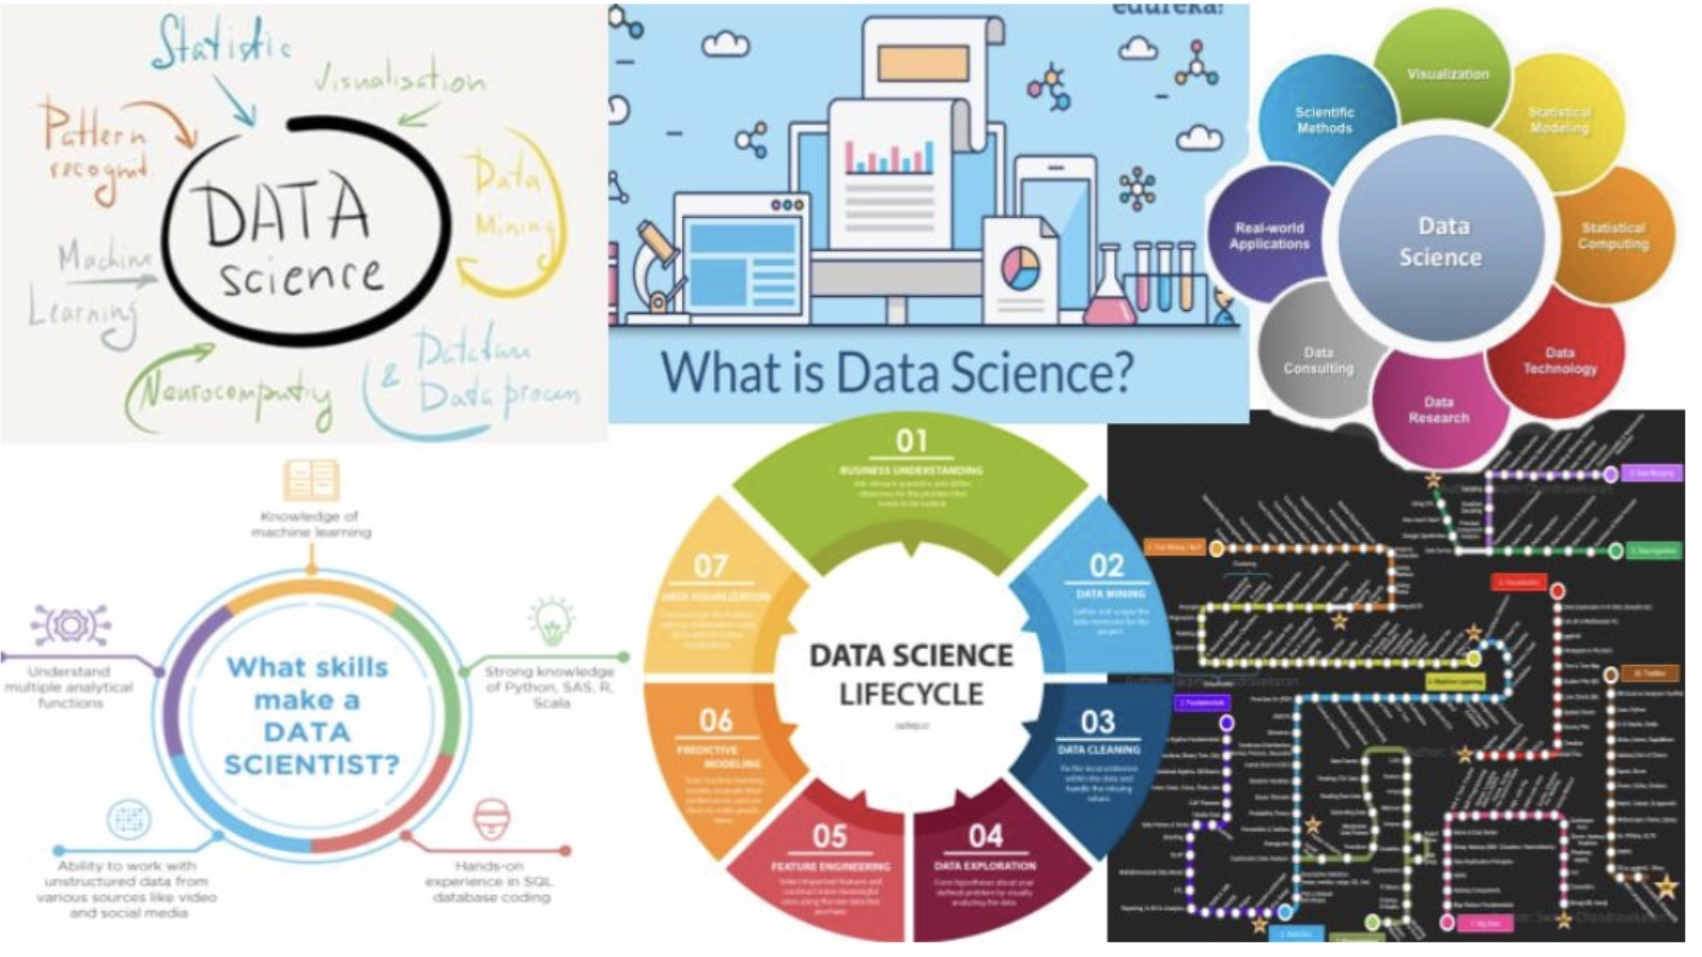
\includegraphics[width=0.6\textwidth,height=\textheight]{./images/WIDS-1.jpg}

The exact definition of Data Science can be a tad fluid. If you ask two
different data scientists, you will get two different answers. The exact
topics, skills, and outcomes could be different from person to person.
However, the general consensus is that Data Science is the practice of
using data to make decisions. This can be done in a variety of ways, but
the most common methods are through the use of statistics and machine
learning.

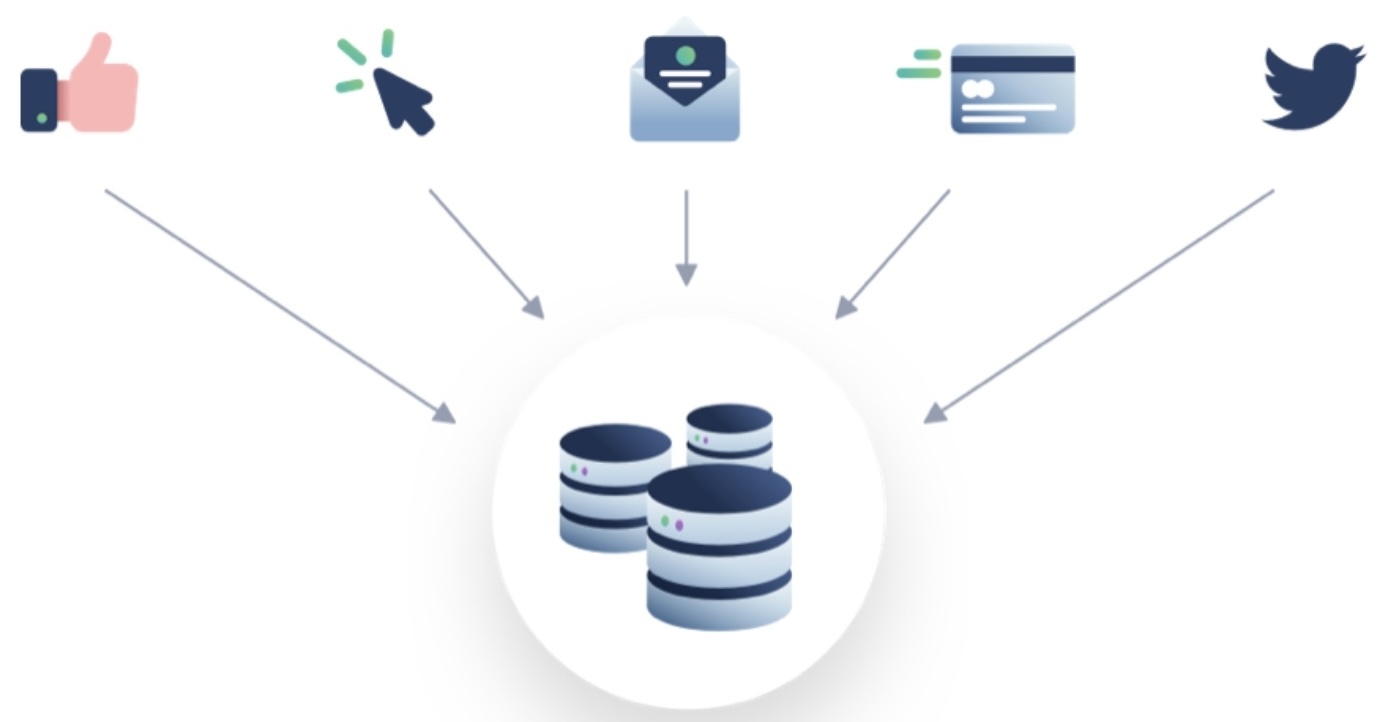
\includegraphics[width=0.6\textwidth,height=\textheight]{./images/WIDS-2.jpg}

Whether we know it or not, we are giving away tons of data every day.
When you ``like'' a social media post, use a search engine, listen to
online music, make an online purchase, or even walk around with your
phone, you are giving away data. This data is collected, stored, and
analyzed by companies to make decisions. These decisions can be as
simple as what ad to show you or as complex as what products to develop.

There are companies that collect data on everything we do. One of the
questions we are going to work through this term is how to start
analyzing this data. If we are a data scientist, what is the procedure
and timeline for analyzing data? What does the typical workflow look
like in the field of data science?

\section*{Step 1 : Data Collection}\label{step-1-data-collection}
\addcontentsline{toc}{section}{Step 1 : Data Collection}

\markright{Step 1 : Data Collection}

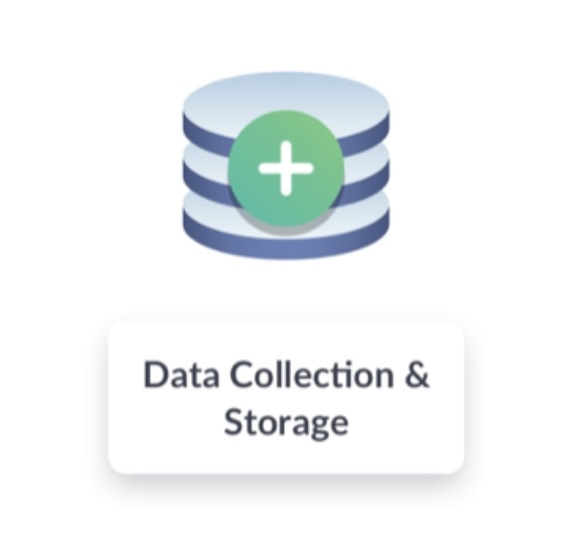
\includegraphics[width=0.25\textwidth,height=\textheight]{./images/WIDS-3.jpg}

The first step is to collect the data. As was mentioned above, this can
be done in a variety of ways. The data can be collected from a variety
of sources, some of which are going on and we don't even know it. The
data can be collected from a variety of sources, from the internet, to
social media, to smart devices, and even from the government. The data
can be collected in a variety of ways, from surveys, to interviews, to
observations, to experiments. The data can be collected in a variety of
formats, from text, to images, to audio, to video. Once the data
collection process is completed, the job of a data scientist is to take
this data and find what story it is trying to tell.

\section*{Step 2 : Data Preparation}\label{step-2-data-preparation}
\addcontentsline{toc}{section}{Step 2 : Data Preparation}

\markright{Step 2 : Data Preparation}

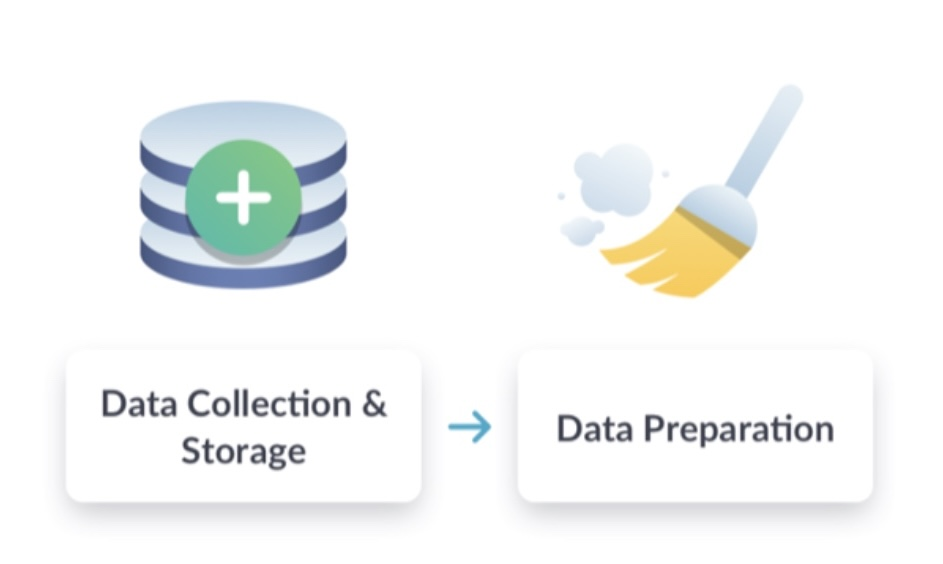
\includegraphics[width=0.4\textwidth,height=\textheight]{./images/WIDS-4.jpg}

If you talk with someone who is a data scientist, they will undoubtedly
tell you that the majority of their time is spent preparing the data.
This is because the data is often messy and needs to be cleaned up
before it can be analyzed. The data needs to bet set up in a way that
the data scientist will be able to analyze it. The data will need to be
set up so that it can be analyzed by a script. That means it needs to be
prepared (often called ``cleaned'') so that the script can read in the
data, label the variables, and start the analysis. We are trying to
structure the data set so that the script can take in the data and start
the anaylsis.

This can be done in a variety of ways, from removing missing data,
combining variables, removing duplicates, dealing with outliers, and
removing irrelevant data. Once the data is cleaned up, the job of a data
scientist is to take this data and find what story it is trying to tell.

\section*{Step 3 : Exploration and
Visualization}\label{step-3-exploration-and-visualization}
\addcontentsline{toc}{section}{Step 3 : Exploration and Visualization}

\markright{Step 3 : Exploration and Visualization}

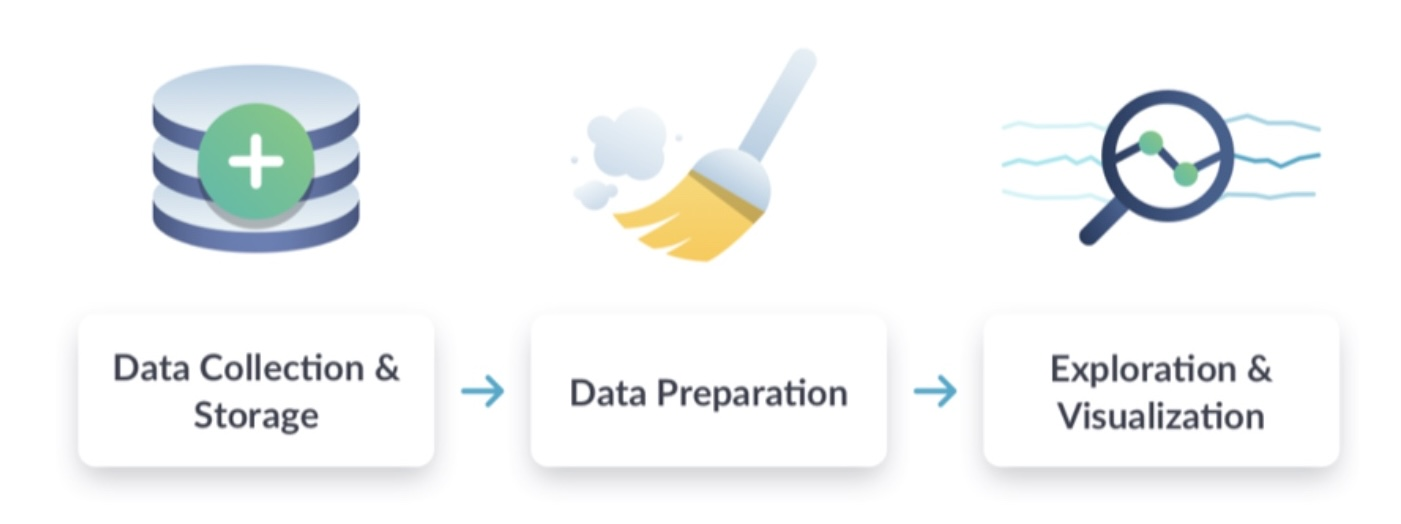
\includegraphics[width=0.55\textwidth,height=\textheight]{./images/WIDS-5.jpg}

Once the data is cleaned up, the data scientist will start to explore
the data. This can be done in a variety of ways, from looking at the
data in a table, looking at the data in a graph, or perhaps looking at
the data in a map. The data scientist will start to look at the data
with many different tools to see what story it is trying to tell.

Traditionally, the data scientist will start by looking at the data in a
table or a graph. This initial look at the data will help the data
scientist to see if there are any obvious patterns or trends in the
data. If there are, then the data scientist will start to explore these
patterns or trends in more detail.

For example, conside the story \textbf{Little Women}. The following
graph shows the cumulative number of times the names of the main
characters are used in the book.

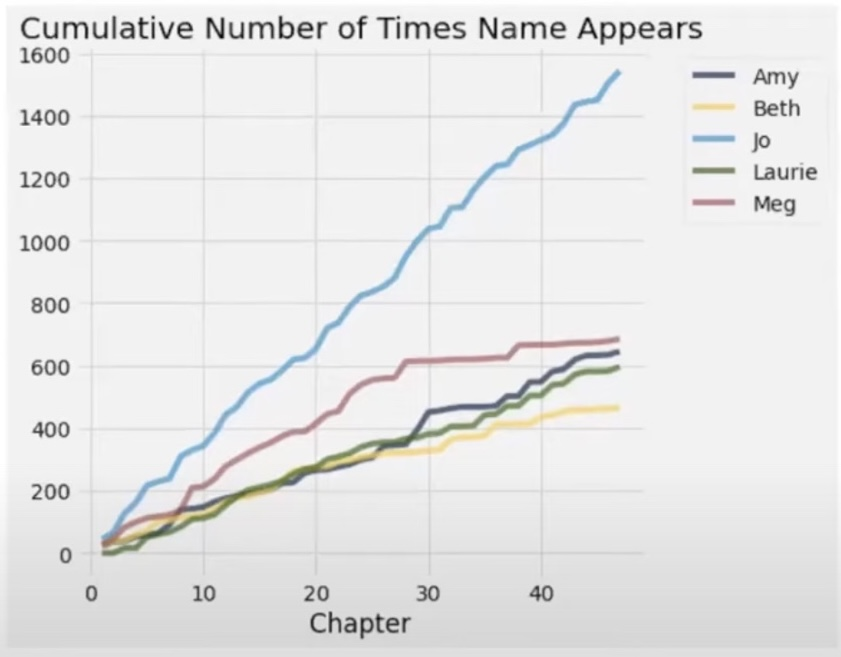
\includegraphics[width=0.4\textwidth,height=\textheight]{./images/WIDS-6.jpg}

The graph shows that the name ``Jo'' is used the most, followed by
``Meg'', ``Amy'', and ``Laurie''. If we were going to ask the question
of who the main character is in the book, the data would suggest that
the protagonist of the story is Jo. Her name appears the most in the
book, and it is not very close.While this is an interesting idea to
consider, we could also delve a little deeper at this graph. In the
story, two of the five characters listed get married to one another.
Based on this graph, can we hypothesize as to whom those two people
might be?

Based on the graph, we could hypothesize that Amy and Laurie get
married. If we examine the graph, we can see that the pattern for the
number of times Amy appears in the book is very similar to the pattern
for the number of times Laurie appears in the book starting around
chapter 35. This could suggest that the two of them are in several
scenes at the same time and when one is mentioned, then the other is
also there. Thus they are starting to spend more time together.

This proves to be true as Amy and Laurie get married in chapter 44.

\section*{Step 4 : Experimentation and
Prediction}\label{step-4-experimentation-and-prediction}
\addcontentsline{toc}{section}{Step 4 : Experimentation and Prediction}

\markright{Step 4 : Experimentation and Prediction}

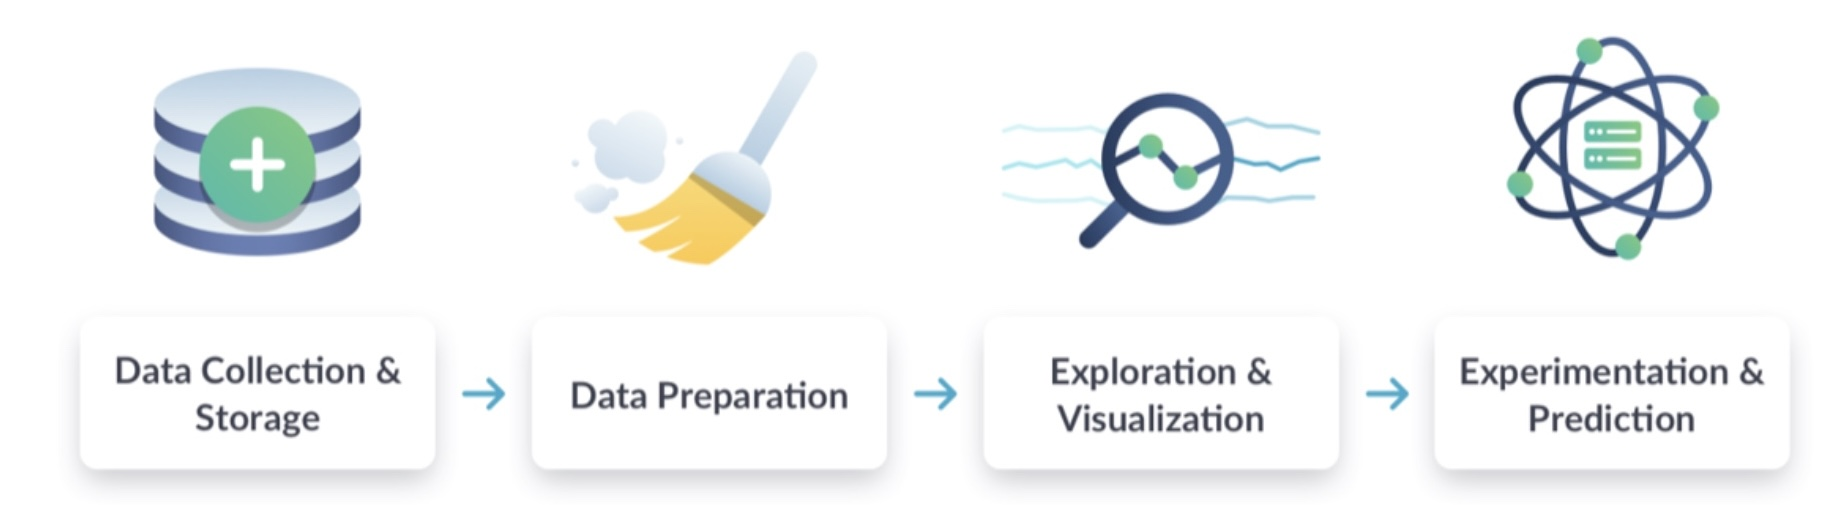
\includegraphics[width=0.7\textwidth,height=\textheight]{./images/WIDS-7.jpg}

One of the goals of a data scientist is to take data and try to figure
out what comes next.

\begin{itemize}
\tightlist
\item
  Is a stock going to rise or fall?
\item
  Is a virus going to continue to spread or die out?
\item
  Is a customer going to buy a product?
\end{itemize}

These are all questions that a data scientist will try to answer. We are
now at the stage of trying to make predictions based on the data that we
have collected, cleaned, and explored. A data scientist will make a
``Model'' that will try to predict what comes next. When we say
``model'', are really saying a mathematical equation that represents the
data set. This model will be used to make predictions about the future.
There are several ways to make a model, but this course will focus
primarily on what is know as ``linear regression''. This is a beginning
modelling technique that will introduce you to the modelling concept and
get you started on the path to making predictions.

\section*{Step 5 : Learning Goals}\label{step-5-learning-goals}
\addcontentsline{toc}{section}{Step 5 : Learning Goals}

\markright{Step 5 : Learning Goals}

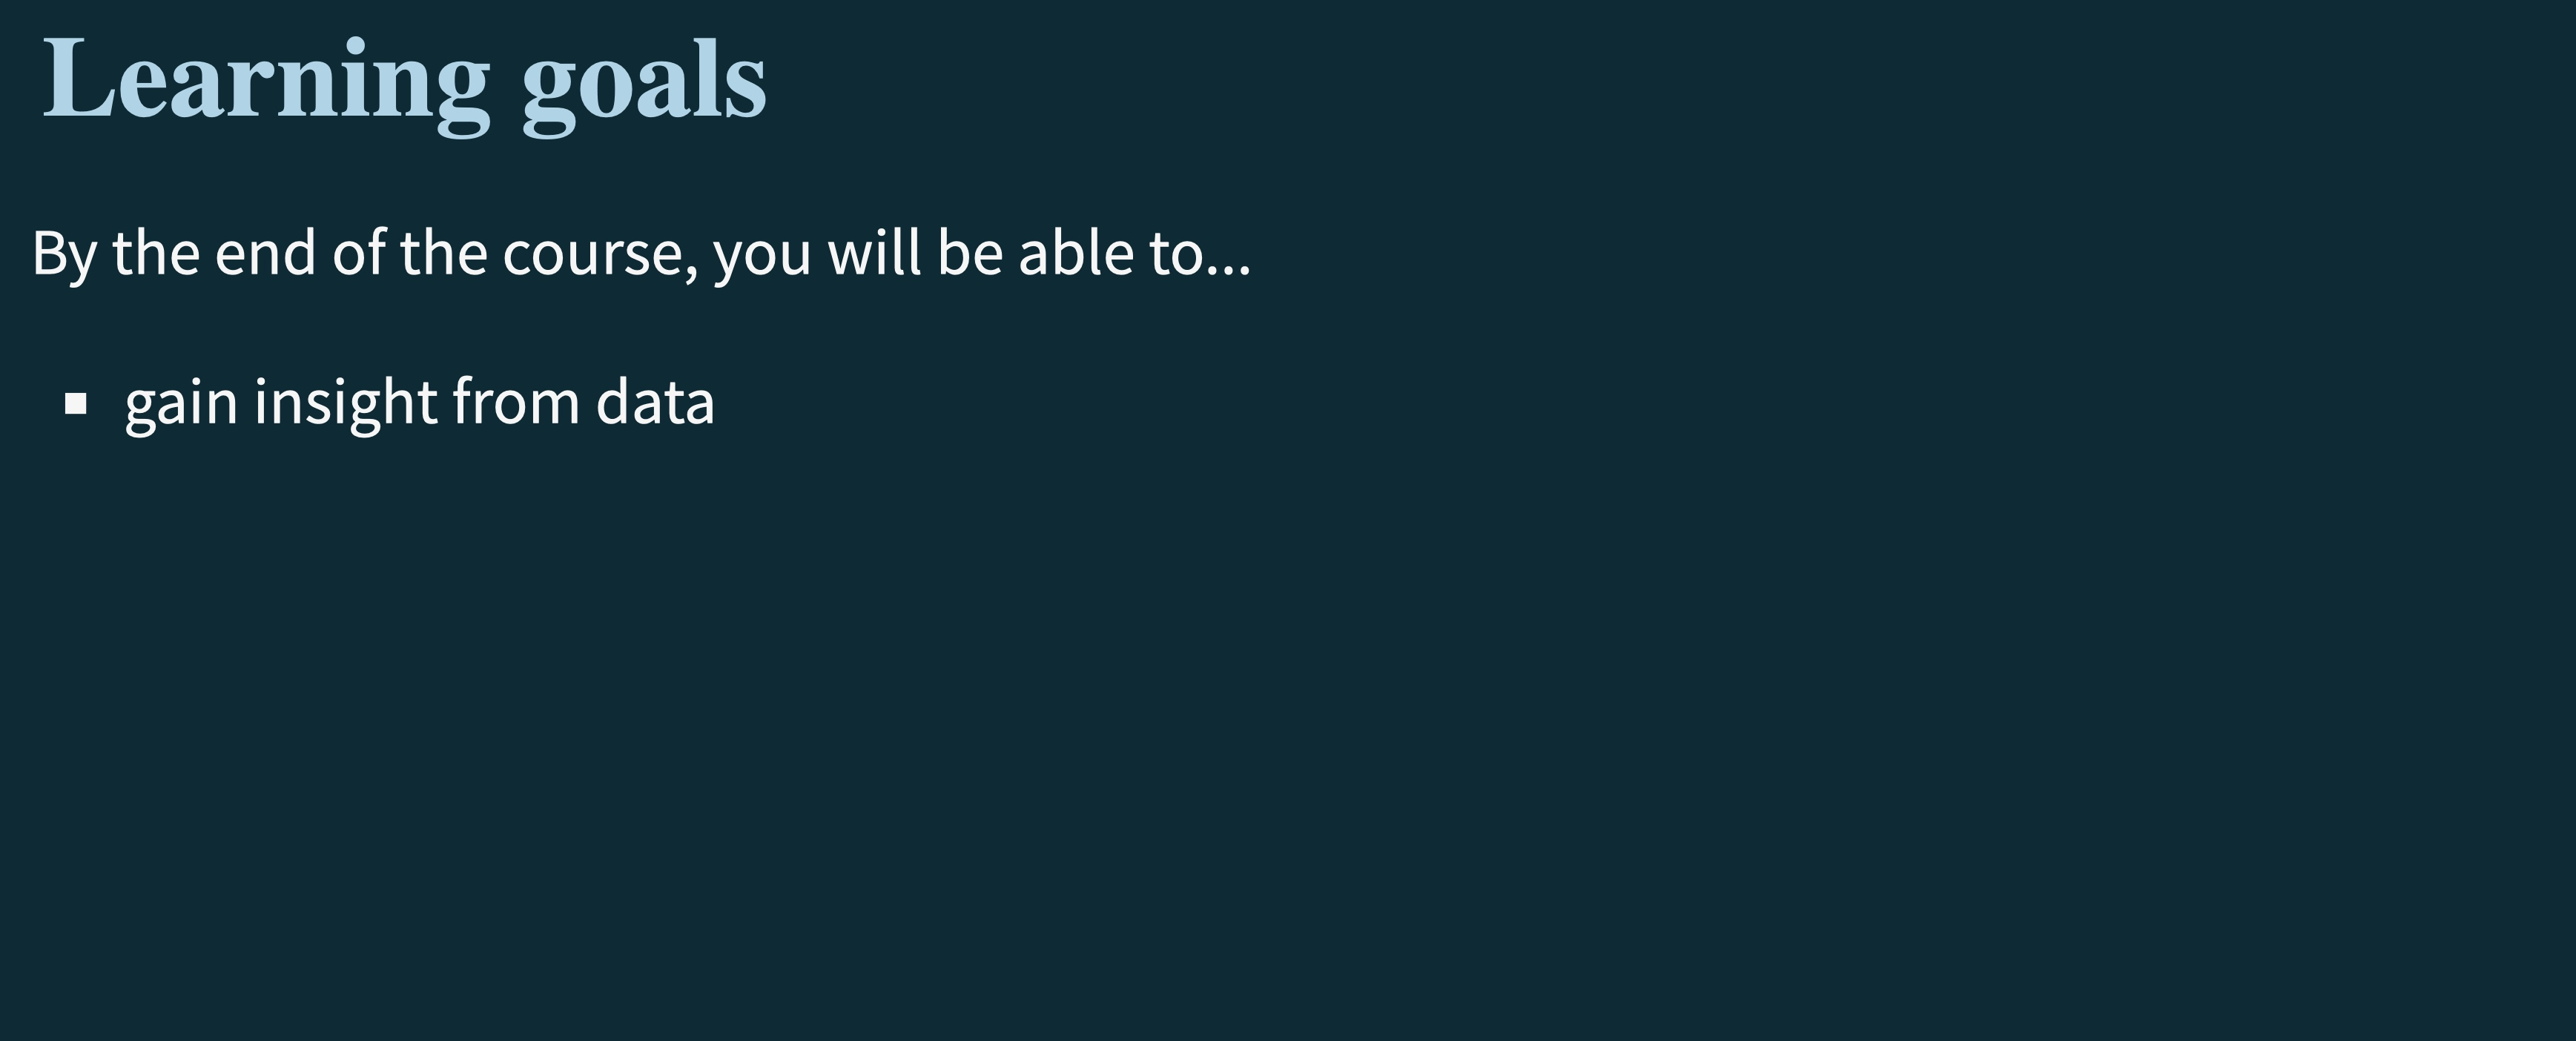
\includegraphics[width=0.6\textwidth,height=\textheight]{./images/WIDS-8.jpg}

As we walked through above, one of the main goals of this course is for
you to be able to take in a data set and find some story that it is
trying to tell. In other words, what insights can you pull out of a data
set?

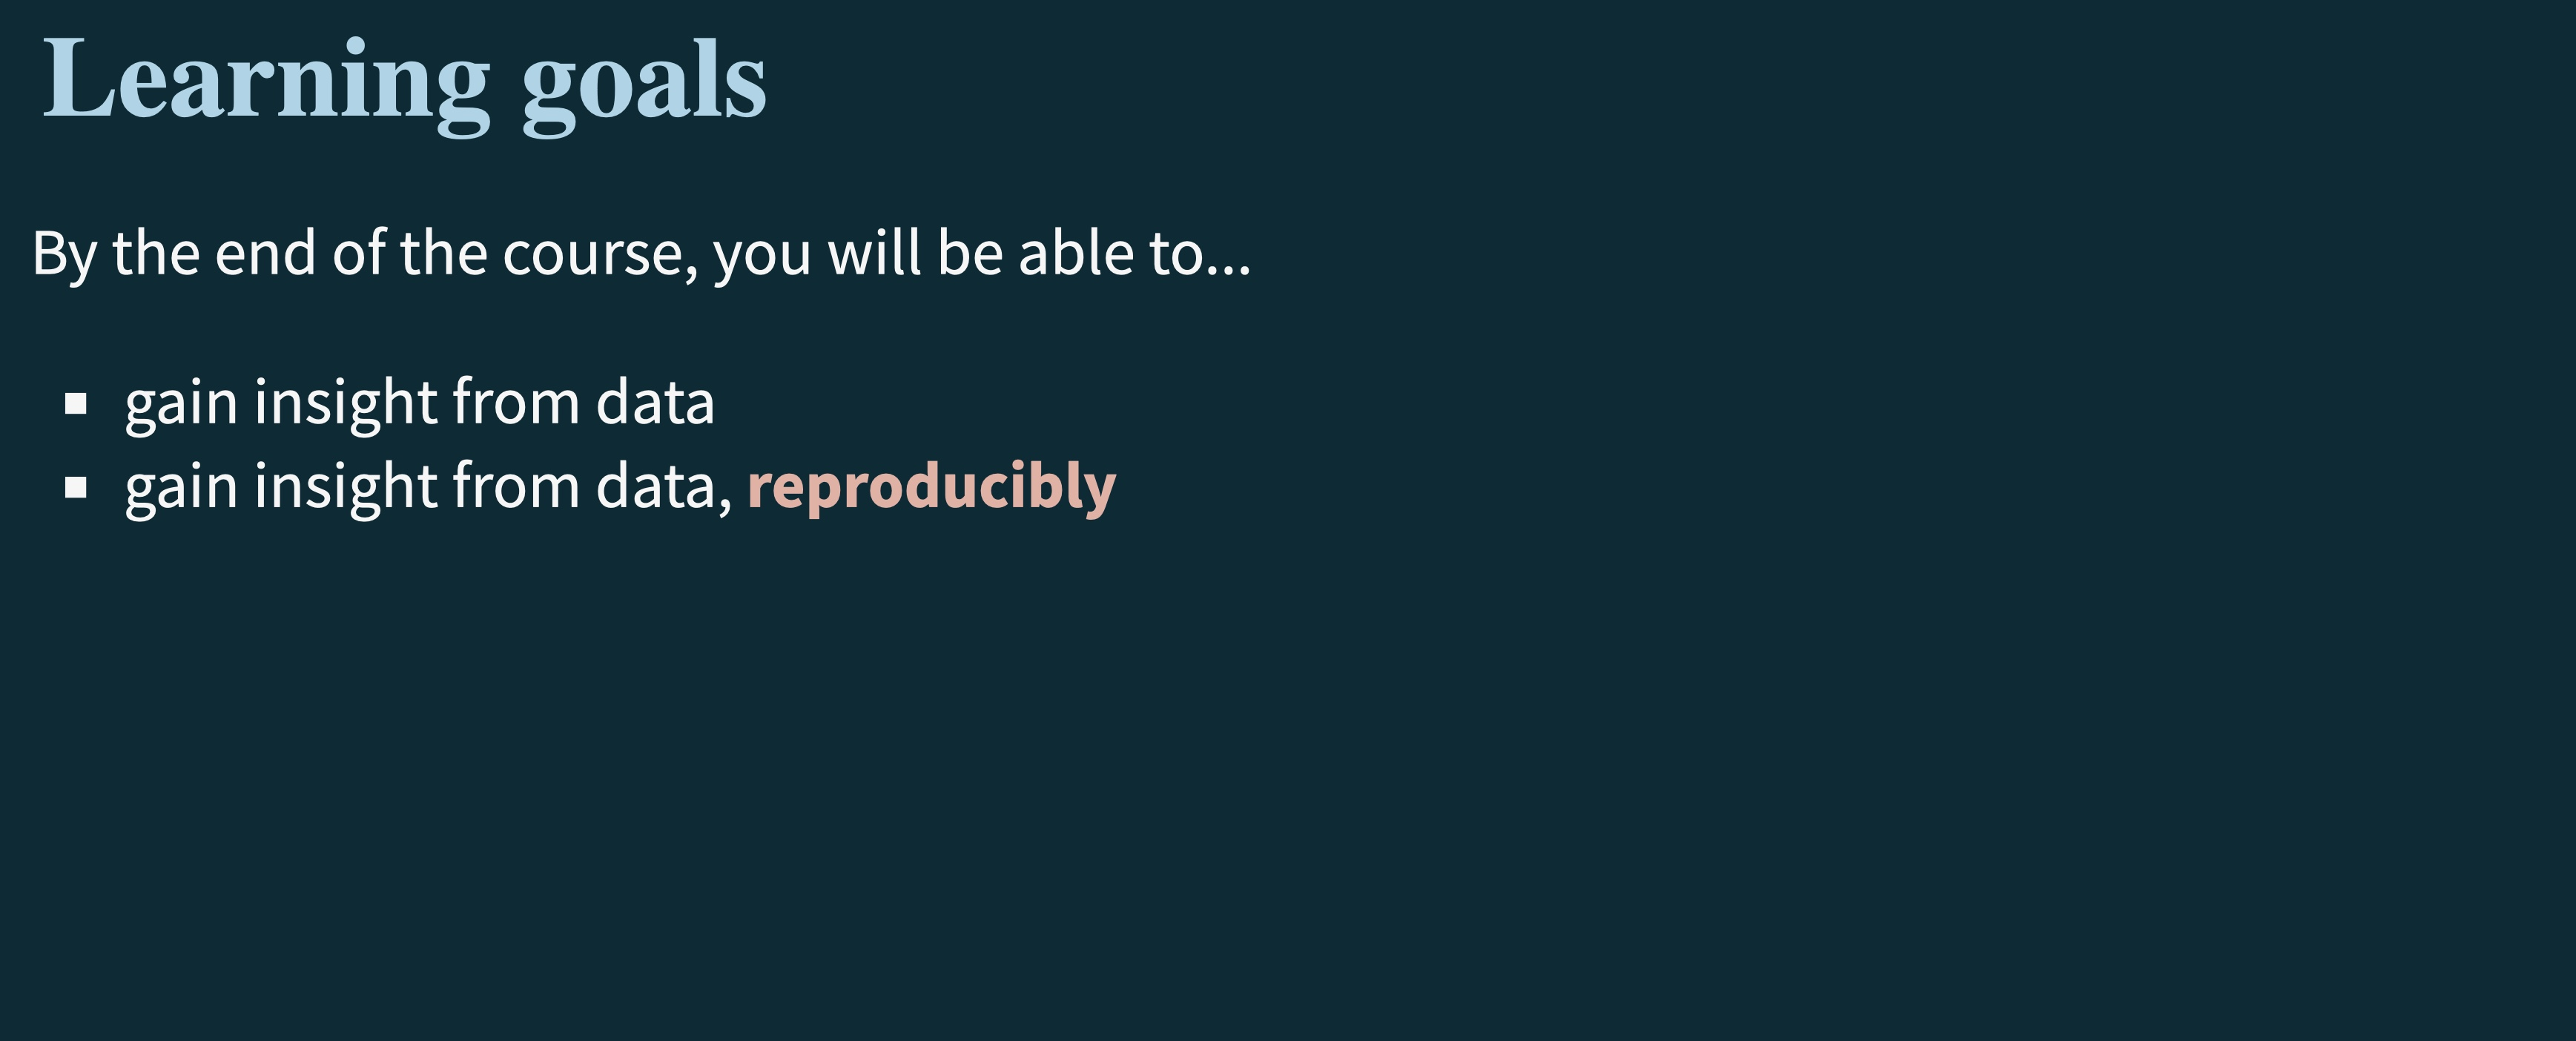
\includegraphics[width=0.6\textwidth,height=\textheight]{./images/WIDS-9.jpg}

If a data scientist, or any scientist for that matter, wants their work
to be taken seriously, then it needs to be reproducible. This means that
if you were to take the data set and the script that was used to analyze
the data, you should be able to get the same results. This is a big part
of the scientific method. If you can't reproduce the results, then the
results can not be considered reliable or valid.

For our consideration, what does it mean for work to be
``reproducible''?

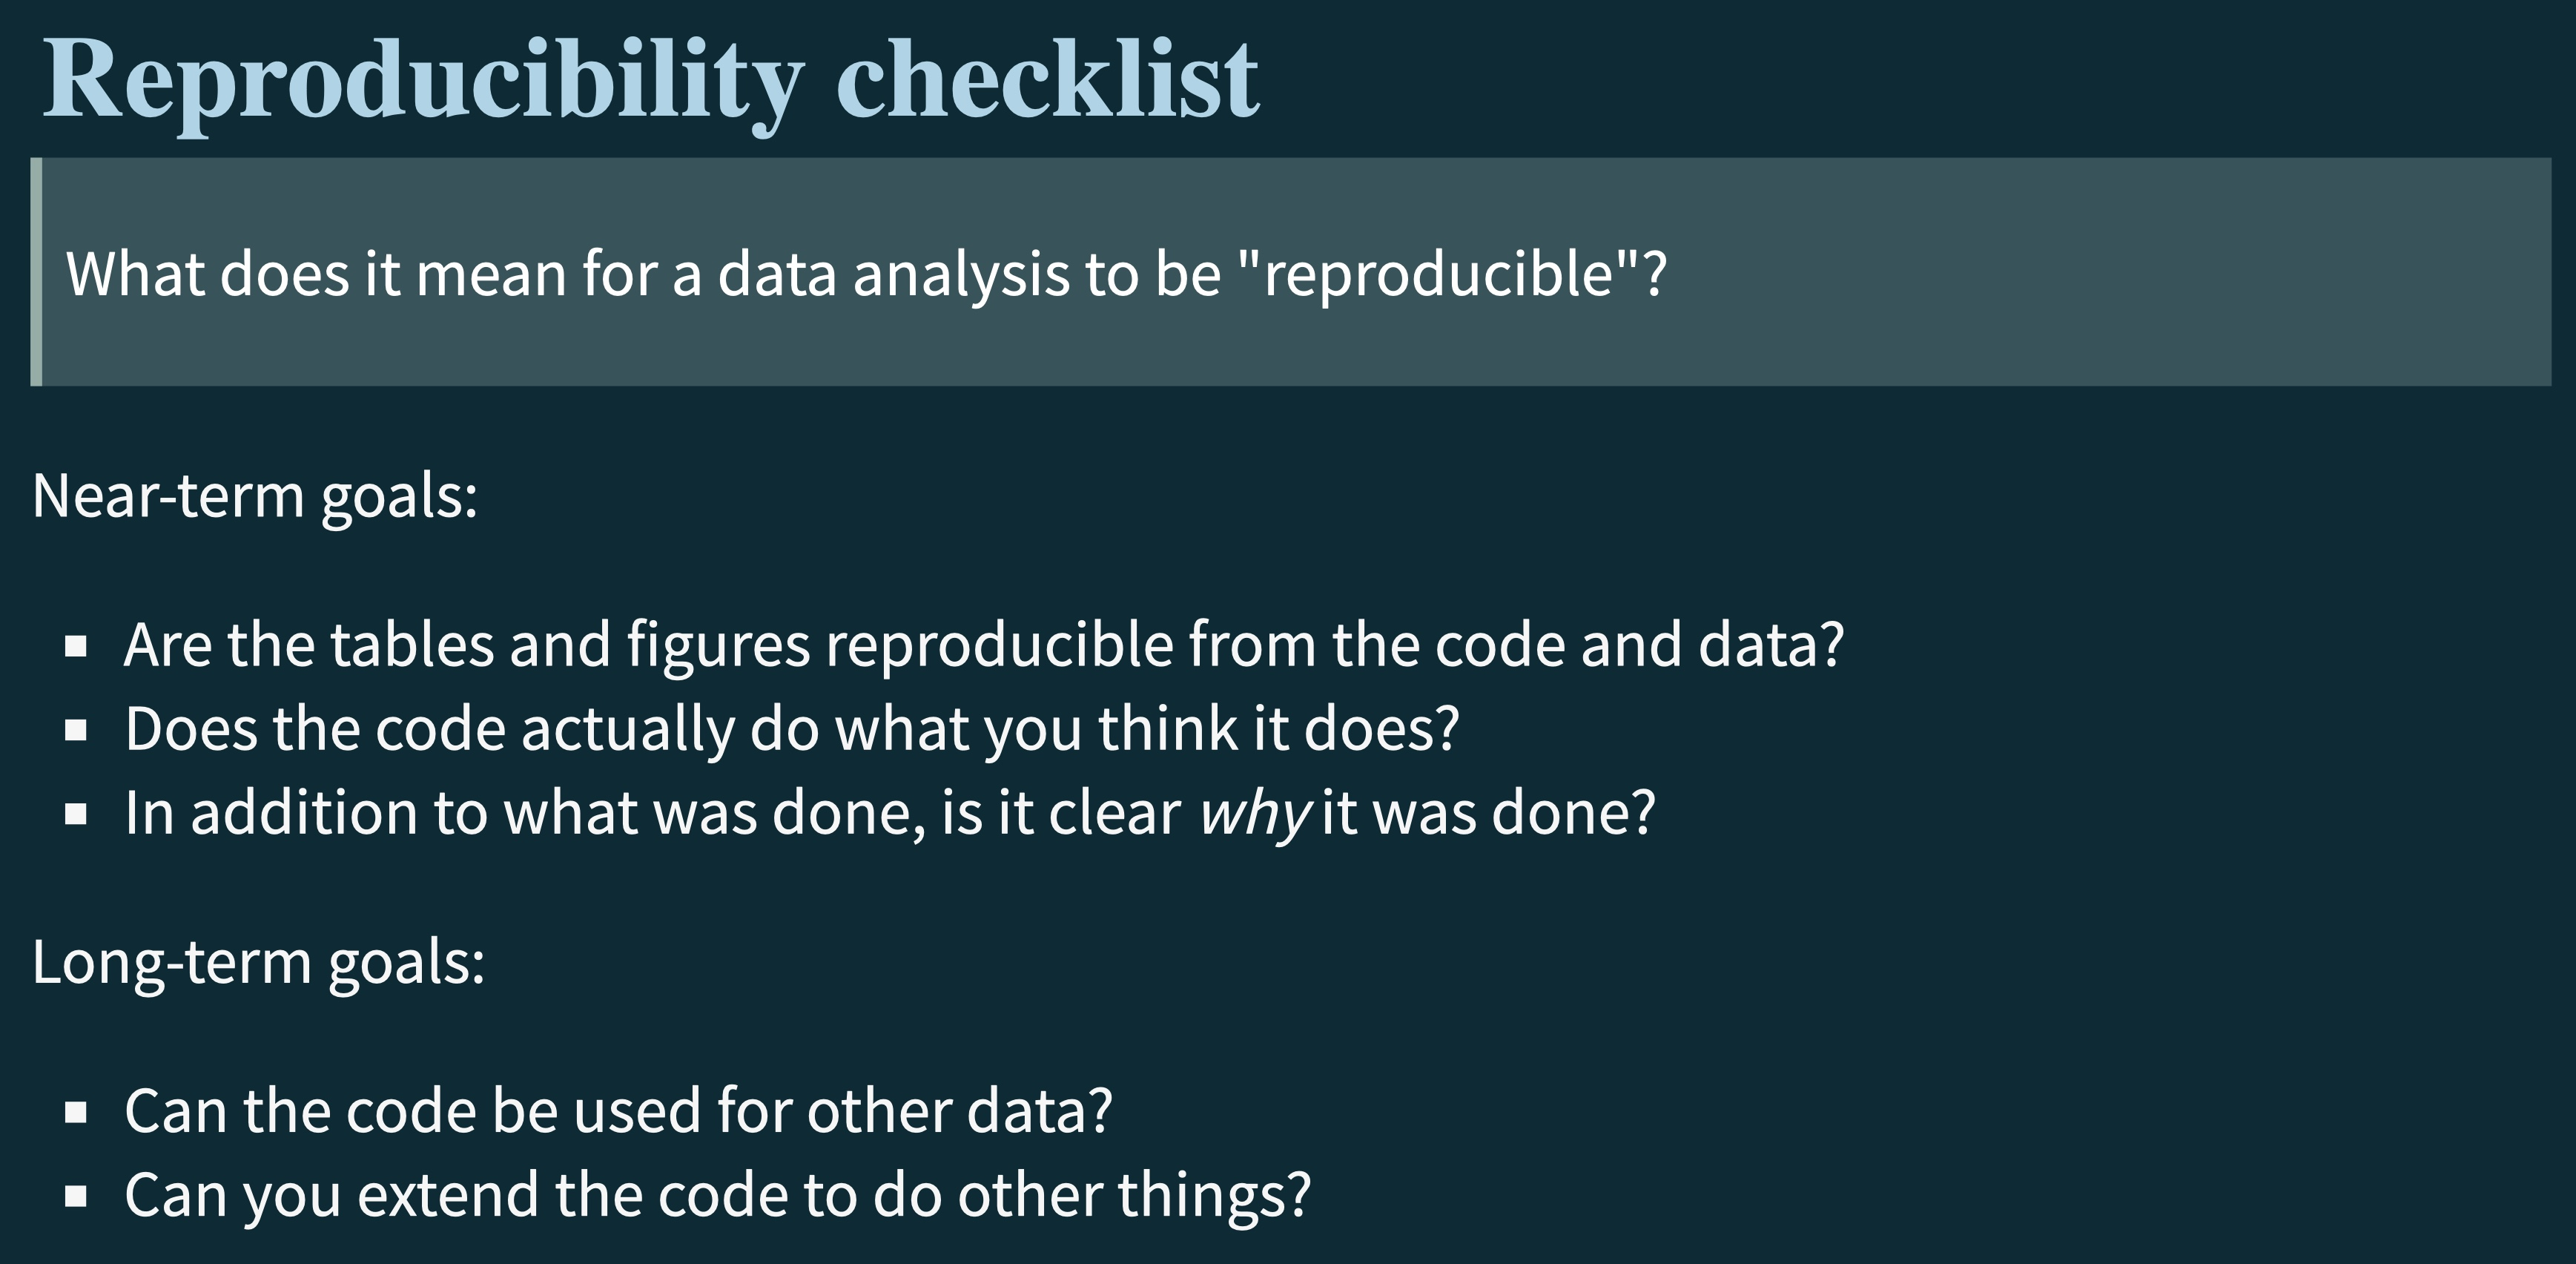
\includegraphics[width=0.6\textwidth,height=\textheight]{./images/WIDS-10.jpg}

In the graphic above, the near-term goals show you what to consider for
the project in which you are currently working. The long-term goals show
you what you should be thinking about for the future as you are working
on you current project.

You don't want to be always ``recreating the wheel''. Can you write code
that can be adapted to other data sets easily? Can you write code that
you, or someone else, could modify to find a different story in your
data set or in a different data set?

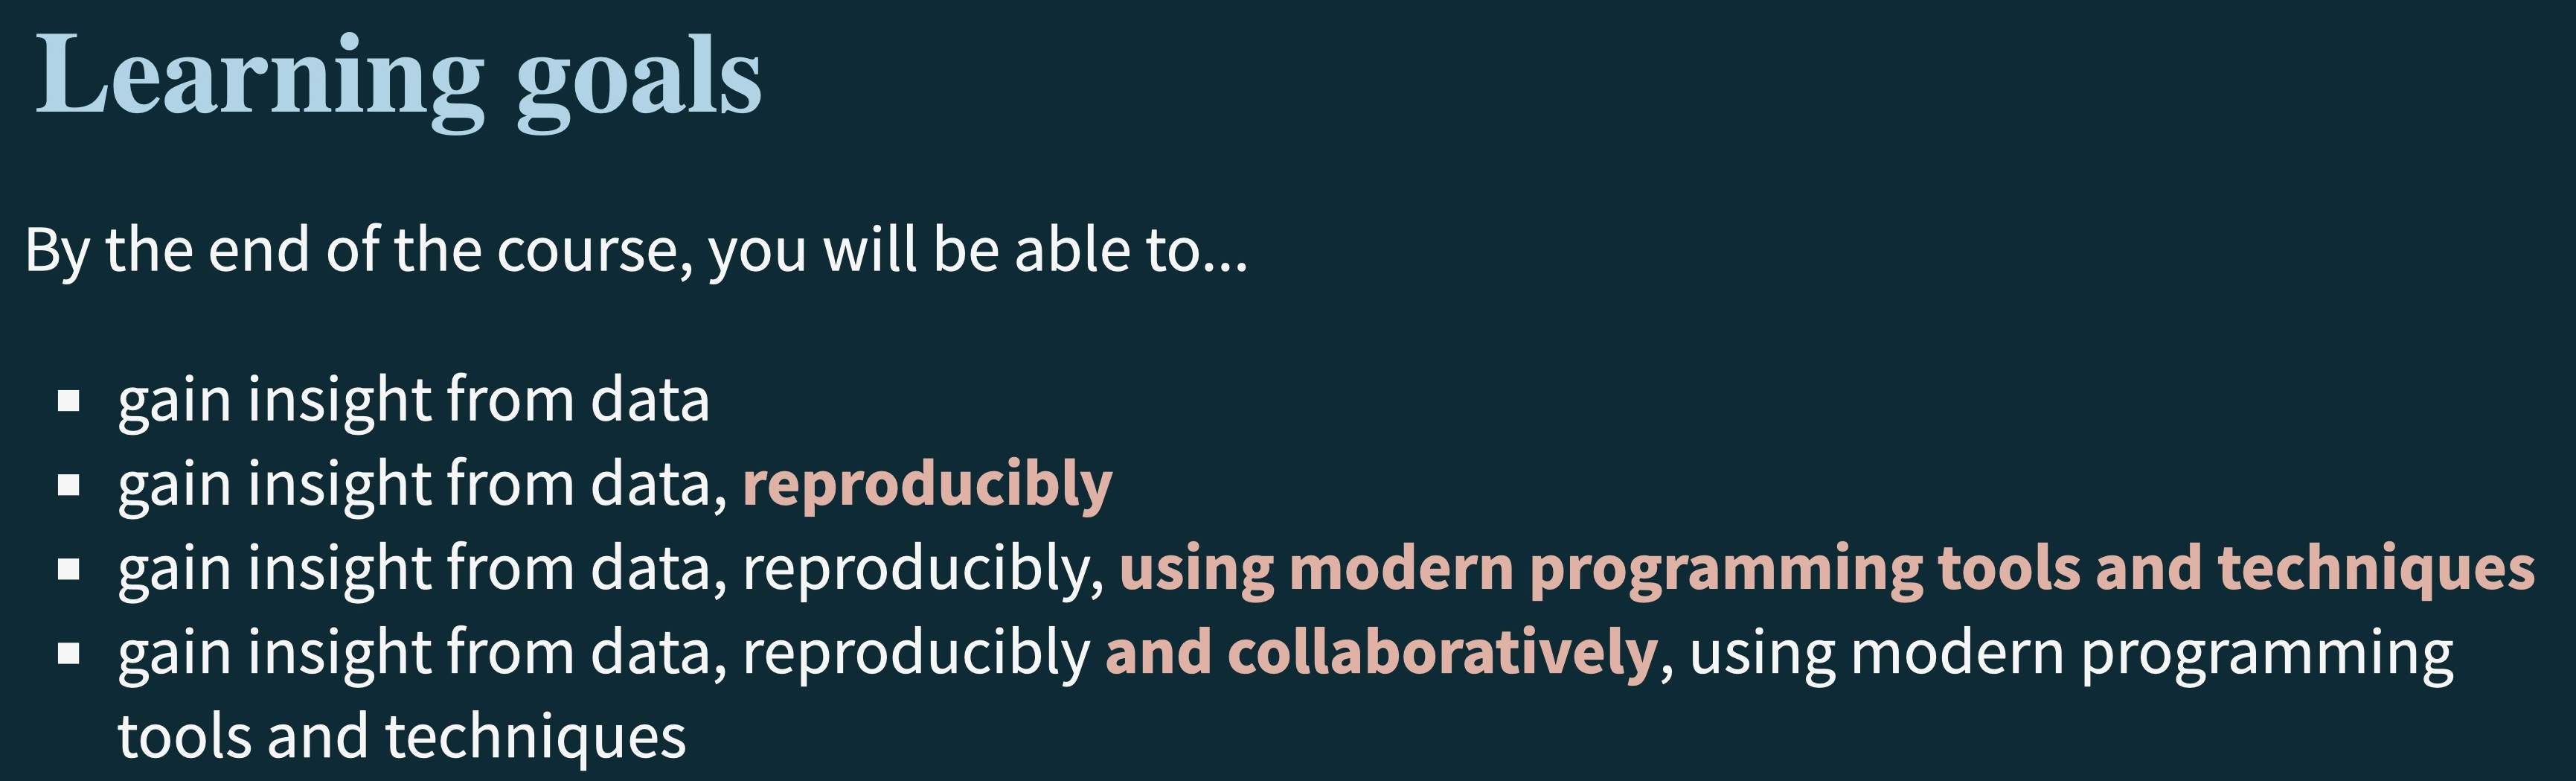
\includegraphics[width=0.6\textwidth,height=\textheight]{./images/WIDS-12.jpg}

The final two learning goals we will discuss will be working
collaboratively and using the same tools as used by data science
professionals. As you will hear from some of our data scientist guests,
they are almost always working with a group. This group analyses the
data, creates the visualizations, writes code, and finalize reports
together. Being able to work with and listen to others is a skill that
can help you become a better data scientist, better communicator, and
better team member.

When it comes to tools for data analysis, the industry standards are R
and Python. These are the two most common programming languages used by
data scientists. Academic or scientific research is often done in R,
while industry research is often done in Python. If you are going to be
a data scientist, you will need to know how to use these tools. This
course will focus on R, but do not worry if you are worried about not
using python. The two languages are very similar and if you know one,
the other is not too difficult to learn.

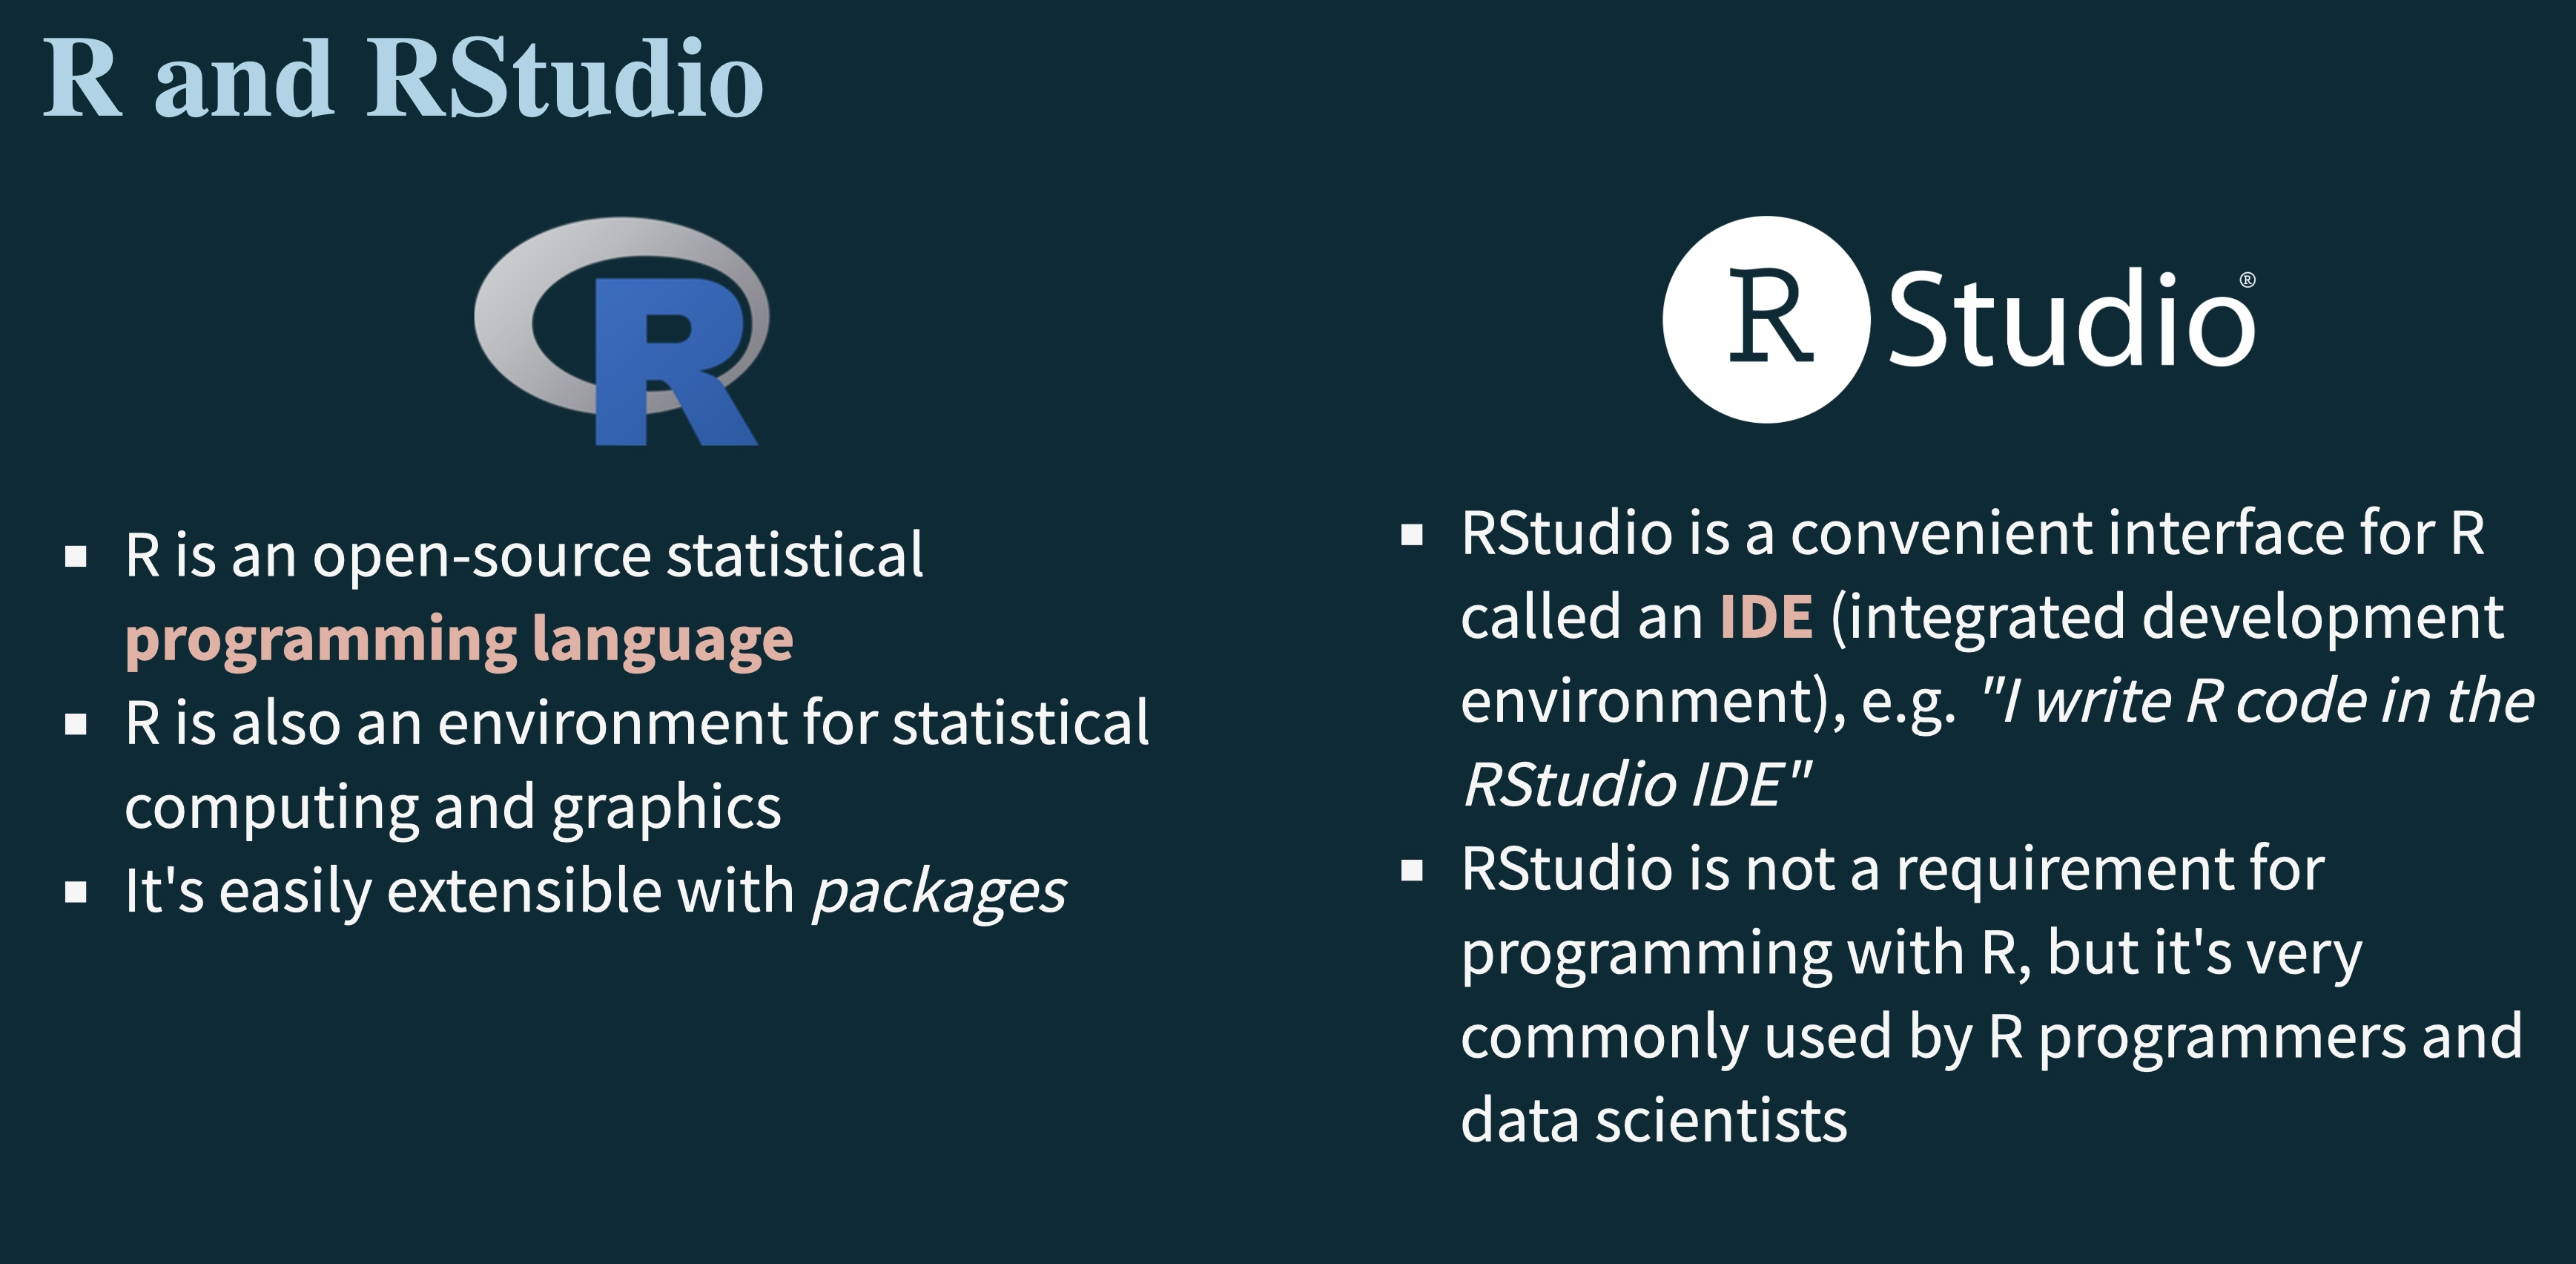
\includegraphics[width=0.6\textwidth,height=\textheight]{./images/WIDS-13.jpg}

\bookmarksetup{startatroot}

\chapter*{What Is Tidyverse}\label{what-is-tidyverse}
\addcontentsline{toc}{chapter}{What Is Tidyverse}

\markboth{What Is Tidyverse}{What Is Tidyverse}

Table with Column Span


\includegraphics[width=1\textwidth,height=\textheight]{./images/WIT_2.jpg}

The tidyverse is a collection of R packages that share an underlying
design philosophy, grammar, and data structures. The tidyverse is
designed to make data science faster, easier, and more fun!
https://www.tidyverse.org

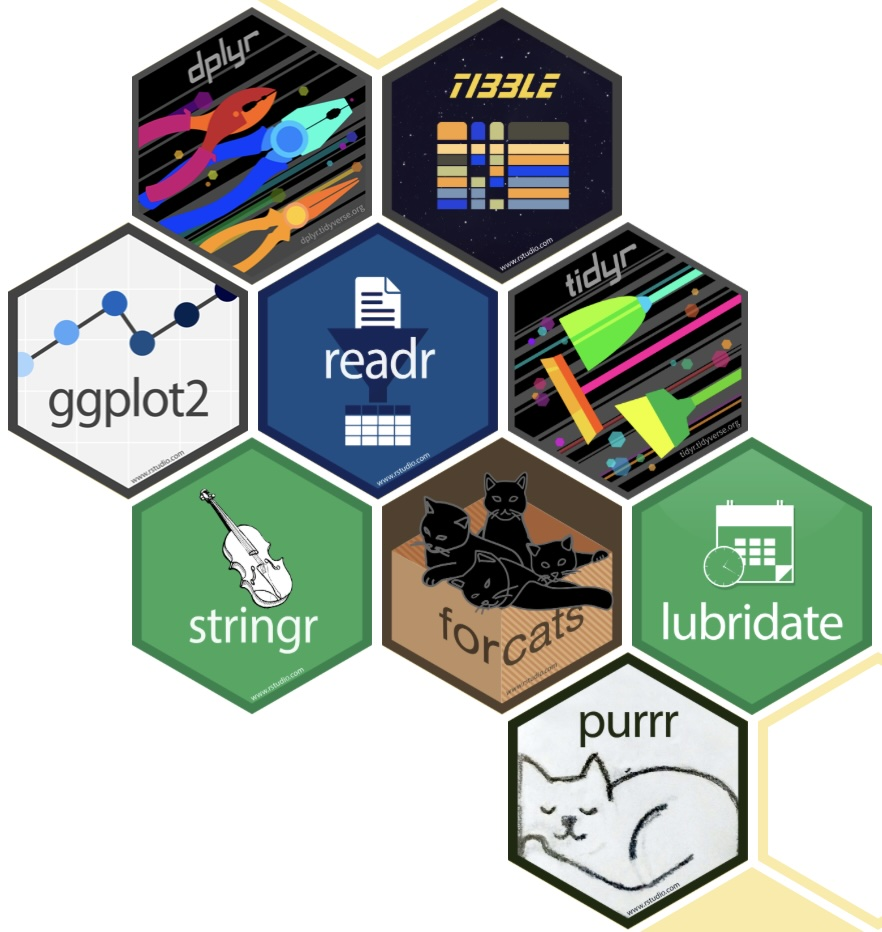
\includegraphics[width=1\textwidth,height=\textheight]{./images/WIT_1.jpg}

Tidyverse is a very important package that contains several other
packages that are used for data manipulation and visualization. This
provides a consistent, efficient, and user-friendly framework for data
manipulation, visualization, and analysis. Here are some key reasons why
learning the tidyverse is beneficial:

\begin{enumerate}
\def\labelenumi{\arabic{enumi}.}
\item
  \textbf{Unified and Consistent Approach :} The tidyverse is a
  collection of R packages (e.g., ggplot2, dplyr, tidyr, readr, purrr,
  tibble) that follow a consistent syntax and philosophy. Functions work
  seamlessly together, reducing the learning curve compared to working
  with disparate R packages.
\item
  \textbf{Data Wrangling Made Easy :} dplyr provides intuitive functions
  like filter(), mutate(), select(), and group\_by() to transform and
  manipulate data efficiently. tidyr helps reshape and clean messy data
  using functions like pivot\_longer(), pivot\_wider(), and separate().
\item
  \textbf{Powerful Data Visualization :} ggplot2 is one of the most
  popular visualization tools, allowing you to create elegant,
  customizable plots using a layered grammar of graphics. ggplot2 makes
  it easy to create complex visualizations with minimal code.
\item
  \textbf{Efficient Data Import \& Export :} readr enables fast reading
  and writing of CSV, Excel, and other data formats without unnecessary
  conversions.
\item
  \textbf{Functional Programming with Purrr :} purrr provides functions
  like map() to perform operations on lists and apply functions
  efficiently.
\item
  \textbf{Reproducibility and Readability :} The pipe operator
  (\%\textgreater\%) makes code more readable by allowing operations to
  be chained together in a logical sequence. Code written using the
  tidyverse is often easier to understand and reproduce.
\item
  \textbf{Wide Adoption and Strong Community Support :} The tidyverse is
  widely used in academia, research, and industry, with extensive
  documentation and community support.
\end{enumerate}

By mastering the tidyverse, you can streamline your data science
workflow, making data manipulation, visualization, and analysis more
intuitive and efficient.

\begin{center}\rule{0.5\linewidth}{0.5pt}\end{center}

As we go through this course, you will use several of these packages
many times. Here is a list of the four main tidyverse packages we will
be using in this course:

\subsection*{readr}\label{readr}
\addcontentsline{toc}{subsection}{readr}

The \texttt{readr(\ )} package makes it easy to read in files that
contain data. It can read in files that are in CSV, TSV, XLS, and other
formats. While there are built in base commands that can do this, the
readr package is faster and more consistent.

\subsection*{tibble}\label{tibble}
\addcontentsline{toc}{subsection}{tibble}

The tibble package is a modern version of the data.frame. Tibbles are
easier to read and work with than data.frames. Tibbles also have an
enhanced \texttt{print(\ )} method which makes them easier to use with
large datasets containing complex objects.

We will use the tibble package to create data frames as we learn to read
in data.

\subsection*{dplyr}\label{dplyr}
\addcontentsline{toc}{subsection}{dplyr}

The dplyr package is a grammar of data manipulation. The dplyr package
makes it easy to analyse data using commands such as
\texttt{filter(\ )}, \texttt{select(\ )}, \texttt{mutate(\ )},
\texttt{arrange(\ )}, and \texttt{summarize(\ )}.

We will use the dplyr package to manipulate data frames as we learn to
clean data.

\subsection*{ggplot2}\label{ggplot2}
\addcontentsline{toc}{subsection}{ggplot2}

The \texttt{ggplot2(\ )} package is a grammar of graphics. The ggplot2
package makes it easy to create beautiful and informative plots. This
will be the primary method we will use to create vizualizations in this
course.

We will go over several different types of plots that can be created
using ggplot2.

\begin{center}\rule{0.5\linewidth}{0.5pt}\end{center}

Here are some other tidyverse packages that are not as commonly used in
this course, but are still very important to know:

\subsection*{tidyr}\label{tidyr}
\addcontentsline{toc}{subsection}{tidyr}

The tidyr package makes it easy to tidy data. The tidyr package makes it
easy to convert data from wide to long format.

This type of data cleaning will not be used as much in this course, but
it is a very important concept to understand and is addressed in a more
advanced course.

\subsection*{broom}\label{broom}
\addcontentsline{toc}{subsection}{broom}

The broom package makes it easy to work with statistical models. The
broom package makes it easy to tidy up the output of statistical models.

We will revisit this package when we delve into modelling a data set.

\subsection*{purrr}\label{purrr}
\addcontentsline{toc}{subsection}{purrr}

The purrr package is a functional programming toolkit. The purrr package
makes it easy to work with lists and vectors.

\subsection*{stringr}\label{stringr}
\addcontentsline{toc}{subsection}{stringr}

The stringr package makes it easy to work with strings. The stringr
package makes it easy to manipulate strings.

\subsection*{forcats}\label{forcats}
\addcontentsline{toc}{subsection}{forcats}

The forcats package makes it easy to work with factors. The forcats
package makes it easy to manipulate factors.

\subsection*{lubridate}\label{lubridate}
\addcontentsline{toc}{subsection}{lubridate}

The lubridate package makes it easy to work with dates and times. The
lubridate package makes it easy to manipulate dates and times.

\begin{center}\rule{0.5\linewidth}{0.5pt}\end{center}

\subsection*{Installation}\label{installation}
\addcontentsline{toc}{subsection}{Installation}

To install the tidyverse package, you can use the following command:

\begin{Shaded}
\begin{Highlighting}[]
\CommentTok{\# If needed, you can install tidyverse by using the following command:}

\CommentTok{\# install.packages("tidyverse")}

\CommentTok{\# Once the package is installed, you can load it up using the library command:}

\FunctionTok{library}\NormalTok{(tidyverse)}
\end{Highlighting}
\end{Shaded}

\begin{verbatim}
-- Attaching core tidyverse packages ------------------------ tidyverse 2.0.0 --
v dplyr     1.1.4     v readr     2.1.5
v forcats   1.0.0     v stringr   1.5.1
v ggplot2   3.5.1     v tibble    3.2.1
v lubridate 1.9.4     v tidyr     1.3.1
v purrr     1.0.2     
-- Conflicts ------------------------------------------ tidyverse_conflicts() --
x dplyr::filter() masks stats::filter()
x dplyr::lag()    masks stats::lag()
i Use the conflicted package (<http://conflicted.r-lib.org/>) to force all conflicts to become errors
\end{verbatim}

You can see that we now have access to the packages that we described
above and by looking at the \texttt{Packages} tab in RStudio. You can
see that the tidyverse package is loaded up and ready to use.

\subsection*{Conclusion}\label{conclusion}
\addcontentsline{toc}{subsection}{Conclusion}

This is one of the more important packages to get to know if you want to
become a data scientist. This package is constantly being updated and
improved, so it is important to stay up to date with the latest changes.

You can find the latest updates and information on the tidyverse
website:

https://www.tidyverse.org

\bookmarksetup{startatroot}

\chapter*{Statistics Language}\label{statistics-language}
\addcontentsline{toc}{chapter}{Statistics Language}

\markboth{Statistics Language}{Statistics Language}

As we start to consider analyzing data, we need to be able to
communicate with other data scientists. This is where statistics
language comes in. We want to take some time to define some terms that
we will be using throughout the course. For now we will just focus on
foundational terms. As we develop different analytic skills, we will
introduce more terms.

\section*{Population}\label{population}
\addcontentsline{toc}{section}{Population}

\markright{Population}

The population is the entire group that we are interested in studying.
For example, if we are interested in studying the average height of all
people in the United States, then the population would be all people in
the United States.

\section*{Parameter}\label{parameter}
\addcontentsline{toc}{section}{Parameter}

\markright{Parameter}

A parameter is a number that describes a population. For example, the
average height of all people in the United States is a parameter. Two of
the more common parameters are the mean and the standard deviation.
These are used to describe the central tendency and the spread of a
population. The mean is typically denoted by the Greek letter mu (μ) and
the standard deviation is typically denoted by the Greek letter sigma
(σ). We will briefly talk about these measures below and go into more
detail in later sections.

Many studies that are done are ones that are trying to estimate a
parameter. Unfortunately, there is only one way to know the true value
of a parameter and that is to measure the entire population. This is not
feasible in most cases as the amount of time and resources to contact
every member of a population is not practical. We can, however, take
what is called a sample of the population and use that to estimate the
parameter.

\section*{Sample}\label{sample}
\addcontentsline{toc}{section}{Sample}

\markright{Sample}

A sample is a subset of the population. For example, if we are
interested in studying the average height of all people in the United
States, then a sample could be a group of 100 people from the United
States. This is a much easier way to get information about the
population rather than having to contact every member of the population.

There are several different methods one can use to take a sample. We
will discuss these methods in later sections.

\section*{Statistic}\label{statistic}
\addcontentsline{toc}{section}{Statistic}

\markright{Statistic}

A statistic is a number that describes a sample. For example, the
average height of a group of 100 people from the United States is a
statistic. Two of the more common statistics are the sample mean and the
sample standard deviation. These are used to describe the central
tendency and the spread of a sample. The sample mean is typically
denoted by the letter x-bar (x̄) and the sample standard deviation is
typically denoted by the letter s.

If we are trying to answer a question about the population, for instance
the average height of all people in the United States, we can take a
sample of the population and use the value from the sample as an
estimate for the parameter from the population. This is the basis of
inferential statistics, which we mention next.

\section*{Inferential Statistics}\label{inferential-statistics}
\addcontentsline{toc}{section}{Inferential Statistics}

\markright{Inferential Statistics}

Inferential statistics are used to make inferences from a sample to a
population. In other words, inferential statistics are used to make
predictions about a population based on a sample. The following graphic
demonstrates the process.

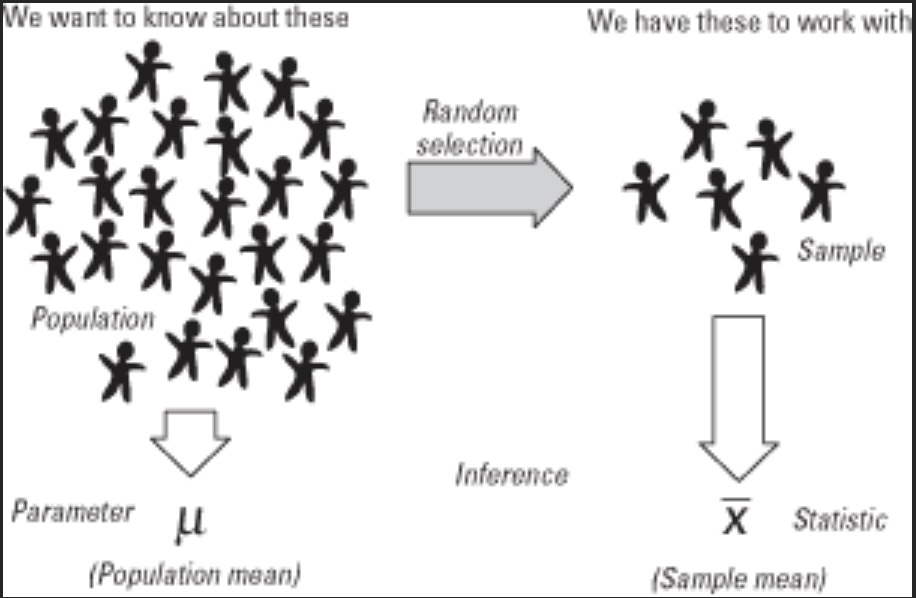
\includegraphics[width=0.4\textwidth,height=\textheight]{./images/SL_1.jpg}

\begin{itemize}
\tightlist
\item
  We are wanting to determine a population parameter μ
\item
  We take a sample from the population
\item
  Calculate the value of the statistic x̄ from the sample.
\item
  Use the sample statistic x to estimate the population parameter μ.
\end{itemize}

This process is the basis of inferential statistics. Using the sample to
help us determine estimates of the population parameter.

\section*{Descriptive Statistics}\label{descriptive-statistics}
\addcontentsline{toc}{section}{Descriptive Statistics}

\markright{Descriptive Statistics}

Descriptive statistics are used to describe the basic features of the
data in a study. They provide simple summaries about the sample and the
measures. For our purposes we will focus on measures of central tendency
(mean, median, mode) and measures of spread (standard deviation,
variance, 5-Number summary). We will discuss these in more detail in
later sections.

\section*{Confidence Interval}\label{confidence-interval}
\addcontentsline{toc}{section}{Confidence Interval}

\markright{Confidence Interval}

We are using a sample to estimate a population parameter. Unfortunately,
if we were to take multiple samples from the population, we would get
different values for the parameter. This is because the sample is only a
portion of the population. The sample you take the first time is almost
assuredly going to be different from the sample you take the second
time. This means that the statistic from the first sample is going to be
different from the statistic from the second sample.

This is the reason why we will estimate a parameter with a confidence
interval. A confidence interval is a range of values that is likely to
contain the true value of a parameter. For example, a 95\% confidence
interval for the average height of all people in the United States would
be a range of values that is likely to contain the true average height
with 95\% confidence. The confidence interval is based on the sample
statistic and a margin of error. The higher the confidence level, the
wider the confidence interval. We will discuss confidence intervals in
more detail in later sections.

\section*{Distribution}\label{distribution}
\addcontentsline{toc}{section}{Distribution}

\markright{Distribution}

The distribution of a data set tells us two things : the values in the
data set and how often they occur.

Here is an example of a distribution of the number of times a person
goes to the gym in a week.

\begin{Shaded}
\begin{Highlighting}[]
\CommentTok{\# We need the tibble function, so load up the tidyverse package}

\FunctionTok{library}\NormalTok{(tidyverse)}
\end{Highlighting}
\end{Shaded}

\begin{Shaded}
\begin{Highlighting}[]
\CommentTok{\# Create a data frame}

\NormalTok{df }\OtherTok{\textless{}{-}} \FunctionTok{tibble}\NormalTok{(}
  \AttributeTok{gym\_visits =} \FunctionTok{c}\NormalTok{(}\DecValTok{0}\NormalTok{, }\DecValTok{1}\NormalTok{, }\DecValTok{2}\NormalTok{, }\DecValTok{3}\NormalTok{, }\DecValTok{4}\NormalTok{, }\DecValTok{5}\NormalTok{, }\DecValTok{6}\NormalTok{, }\DecValTok{7}\NormalTok{),}
  \AttributeTok{frequency =} \FunctionTok{c}\NormalTok{(}\DecValTok{10}\NormalTok{, }\DecValTok{20}\NormalTok{, }\DecValTok{30}\NormalTok{, }\DecValTok{40}\NormalTok{, }\DecValTok{50}\NormalTok{, }\DecValTok{40}\NormalTok{, }\DecValTok{30}\NormalTok{, }\DecValTok{20}\NormalTok{)}
\NormalTok{)}

\NormalTok{df}
\end{Highlighting}
\end{Shaded}

\begin{verbatim}
# A tibble: 8 x 2
  gym_visits frequency
       <dbl>     <dbl>
1          0        10
2          1        20
3          2        30
4          3        40
5          4        50
6          5        40
7          6        30
8          7        20
\end{verbatim}

In this example, the distribution tells us how many times a person goes
to the gym in a week and how often that occurs. For example, 40 people
go to the gym 3 times a week or 30 people go to the gym 6 times a week.

\section*{Outlier}\label{outlier}
\addcontentsline{toc}{section}{Outlier}

\markright{Outlier}

An outlier is a data point that is significantly different from the
other data points in a dataset. Outliers can have a significant impact
on the results of statistical analyses, especially for means and
standard deviations. Outliers can be caused by errors in data
collection, measurement error, or natural variation in the data.

In the following example, if someone went to the gym 15 times in a week
would be considered an outlier. This is because the number of times a
person goes to the gym in a week is typically between 0 and 7.

Depending on the data set, outliers could occur in either the high or
the low direction.

\section*{Normal Distribution}\label{normal-distribution}
\addcontentsline{toc}{section}{Normal Distribution}

\markright{Normal Distribution}

One of the more typical distributions one will work with is the normal
distribution. A normal distribution is a symmetric unimodal
distributionin which the values are distributed around the mean
according to a bell-shaped curve. The normal distribution is
characterized by its mean and standard deviation. In other words, the
mean and standard deviation determine the shape of the normal
distribution. The mean determines the center of the distribution and the
standard deviation determines the height and width of the distribution.

\section*{Skewness}\label{skewness}
\addcontentsline{toc}{section}{Skewness}

\markright{Skewness}

Once we know the distribution of a data set, we will often draw a
picture of the distribution. One of the descriptors we will look for is
skewness. Skewness is a measure of the asymmetry of a distribution. A
distribution is symmetric if the left and right sides are mirror images
of each other. A distribution is positively skewed (or skewed to the
right)\\
if the right tail is longer than the left tail, and negatively skewed
(or skewed left) if the left tail is longer than the right tail.

Here is a graphic giving examples of each type of skewness.

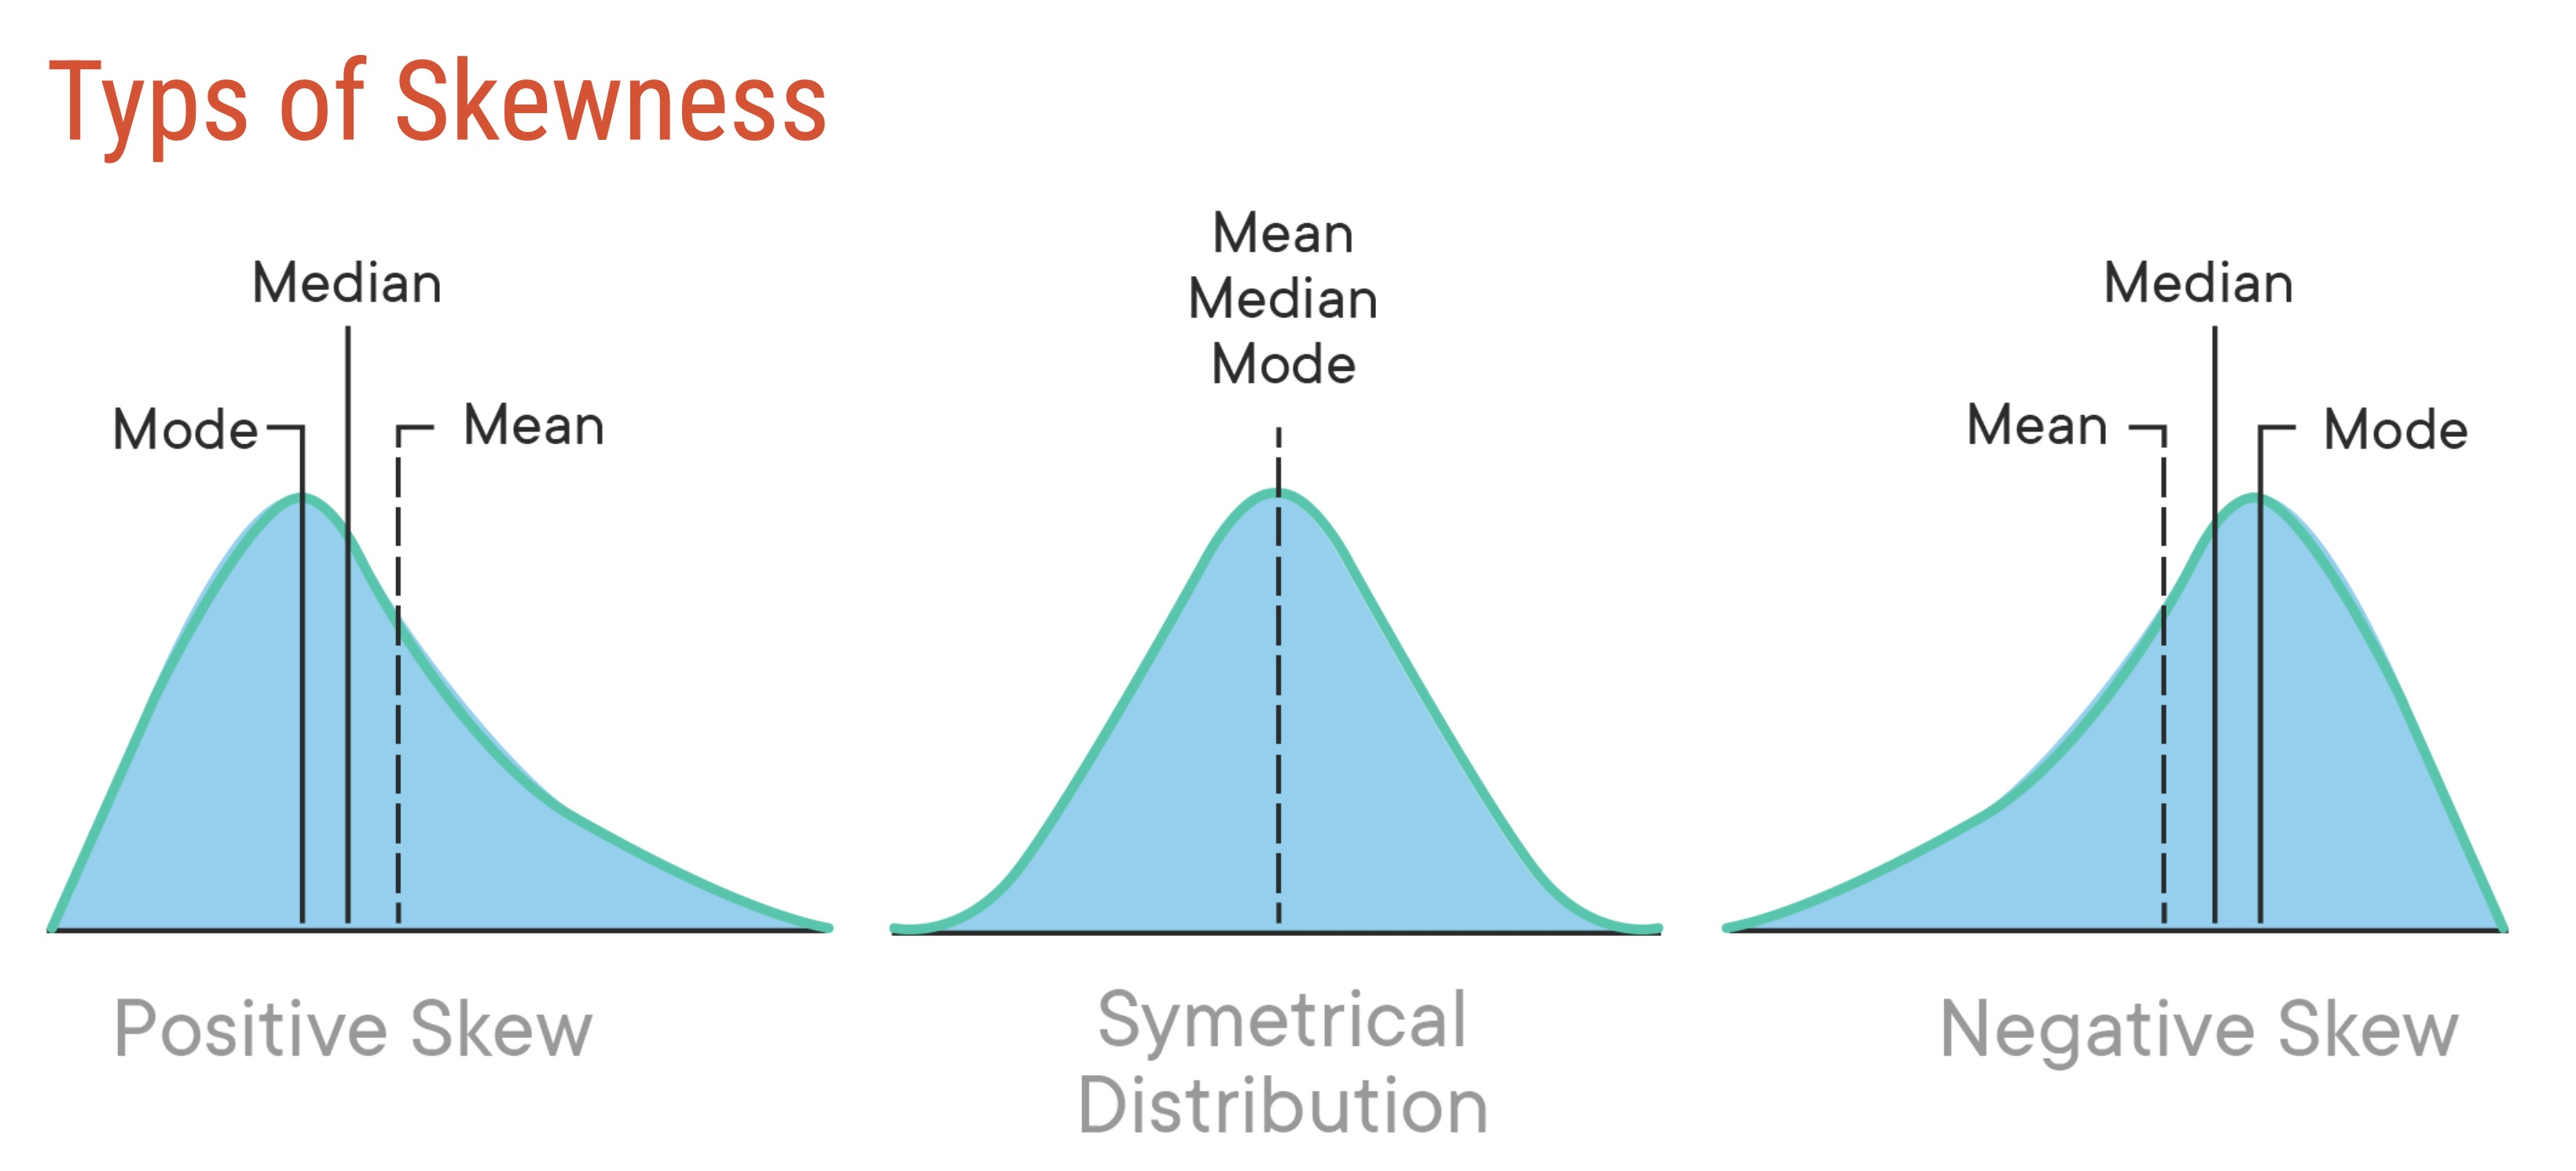
\includegraphics[width=0.6\textwidth,height=\textheight]{./images/SL_2.jpg}

\bookmarksetup{startatroot}

\chapter*{Qualitative and Quantitative
Variables}\label{qualitative-and-quantitative-variables}
\addcontentsline{toc}{chapter}{Qualitative and Quantitative Variables}

\markboth{Qualitative and Quantitative Variables}{Qualitative and
Quantitative Variables}

\section*{Qualitative Variables}\label{qualitative-variables}
\addcontentsline{toc}{section}{Qualitative Variables}

\markright{Qualitative Variables}

Qualitative variables are variables that are not numerical. They are
categorical variables that can be divided into groups, which is why they
are often referred to as \textbf{categorical variables}. You have
probably encountered these when you have filled out an application for
employment. You may have had to check boxes regarding ethnicity, level
of education or gender. These are all examples of qualitative variables.
We can also break them down into two different types of qualitative
variables, \textbf{nominal} and \textbf{ordinal} variables.

\textbf{Nominal} variables are variables that have no order. For
example,

\begin{itemize}
\tightlist
\item
  Hair or Eye Color
\item
  Religious Affiliation
\item
  Gender
\item
  Marital Status
\item
  Political Affiliation
\end{itemize}

Even though these are not numerical variables, we could still create
some numerical structures based off of nominal variables that will help
us understand the data. For example, assume we took a survey of 200
Transylvania University students about their favorite sport to watch and
that 97 said Football, 62 said Basketball, and 41 said Others. Based on
this data, we could create a bar graph to show the distribution of
favorite sports to watch. (Don't worry about knowing these commands yet.
We will get to these commands later in the course.)

We need to first create the data frame for the variable :

\begin{Shaded}
\begin{Highlighting}[]
\CommentTok{\# Create a dataframe. We will first create a vector that has the names}
\CommentTok{\# of the sports and another vector that has the number of students that}
\CommentTok{\# like each sport.}

\NormalTok{sports }\OtherTok{\textless{}{-}} \FunctionTok{c}\NormalTok{(}\StringTok{"Football"}\NormalTok{, }\StringTok{"Basketball"}\NormalTok{, }\StringTok{"Others"}\NormalTok{)}

\NormalTok{students }\OtherTok{\textless{}{-}} \FunctionTok{c}\NormalTok{(}\DecValTok{97}\NormalTok{, }\DecValTok{62}\NormalTok{, }\DecValTok{41}\NormalTok{)}

\CommentTok{\# We will then put them together into a data frame.}

\NormalTok{df }\OtherTok{\textless{}{-}} \FunctionTok{data.frame}\NormalTok{(sports, students)}

\CommentTok{\# And print out the data frame to make sure it looks correct.}

\NormalTok{df}
\end{Highlighting}
\end{Shaded}

\begin{verbatim}
      sports students
1   Football       97
2 Basketball       62
3     Others       41
\end{verbatim}

Even though this data is nominal, we could also create a bar graph to
show the distribution of favorite sports to watch.

\begin{Shaded}
\begin{Highlighting}[]
\CommentTok{\# Create a bar graph using ggplot}

\CommentTok{\# We need to load the ggplot library.}

\FunctionTok{library}\NormalTok{(ggplot2)}

\CommentTok{\# We can now create the bar graph.}

\FunctionTok{ggplot}\NormalTok{(df, }\FunctionTok{aes}\NormalTok{(}\AttributeTok{x =}\NormalTok{ sports, }\AttributeTok{y =}\NormalTok{ students)) }\SpecialCharTok{+} 
  \FunctionTok{geom\_bar}\NormalTok{(}\AttributeTok{stat =} \StringTok{"identity"}\NormalTok{, }\AttributeTok{fill =} \StringTok{"darkred"}\NormalTok{) }\SpecialCharTok{+}
  \FunctionTok{geom\_text}\NormalTok{(}\FunctionTok{aes}\NormalTok{(}\AttributeTok{label =}\NormalTok{ students), }\AttributeTok{vjust =} \SpecialCharTok{{-}}\FloatTok{0.3}\NormalTok{, }\AttributeTok{color =} \StringTok{"black"}\NormalTok{) }\SpecialCharTok{+}
  \FunctionTok{labs}\NormalTok{(}\AttributeTok{title =} \StringTok{"Transy Students Favorite Sports to Watch"}\NormalTok{, }
       \AttributeTok{x =} \StringTok{"Sports"}\NormalTok{, }\AttributeTok{y =} \StringTok{"Number of Students"}\NormalTok{)}
\end{Highlighting}
\end{Shaded}

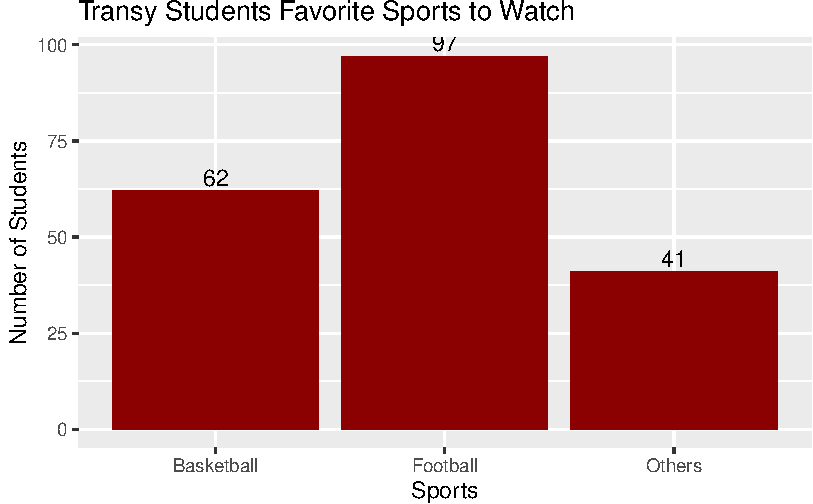
\includegraphics{Qualitative_and_Quantitative_Variables_files/figure-pdf/unnamed-chunk-2-1.pdf}

\textbf{Ordinal} variables are qualitative variables that have an order.
For example, the variable ``education'' is an ordinal variable because
there is an order to the levels of education. They could include the
following:

\begin{itemize}
\tightlist
\item
  educational level (high school, bachelor's, master's)
\item
  clothing size (small, medium, large)
\item
  customer satisfaction rating (dissatisfied, neutral, satisfied)
\item
  pain level (mild, moderate, severe)
\item
  socioeconomic status (low, middle, high).
\end{itemize}

Ordinal variables are often treated as categorical variables, but if it
makes sense, then they can also be treated as numerical variables. What
we would need to do is to assign each of the variables a numerical value
that corresponds to the level of the variable.

We could perform the same commands we did above, but by adding numerical
values to the variables, we might be able to do other meaningful
analysis. For instance, if we were to assign a numerical value to the
levels of education (high school = 1, bachelor's = 2, master's = 3), we
could do something such as calculating the mean level of education for a
group of people.

Notice that we could always add numerical values to qualitative
variables, but it doesn't always make sense to do so. Consider the hair
color example. We could assign value to different outcomes (black = 1,
brown = 2, blonde = 3, etc.) but what would we then do with this data?
It doesn't make sense to calculate the mean hair color of a group of
people, especially if the way you label the numbers to variables is
different from how I would label them. What would the averages describe?
This is why we will call a qualitative variable a \textbf{nominal}
variable if it doesn't make sense to assign numerical values to the
variable, and we will call it an \textbf{ordinal} variable if it does
make sense to assign numerical values to the variable.

\section*{Quantitative Variables}\label{quantitative-variables}
\addcontentsline{toc}{section}{Quantitative Variables}

\markright{Quantitative Variables}

Quantitative variables are numerical variables. Just like the
qualitative variables above, we can be divide quantitative variables
into two different categories, \textbf{discrete} and \textbf{continuous}
variables.

\textbf{Discrete} variables are variables that can only take on certain
values, are countable, and are indivisible. For example, the number of
students in a class is a discrete variable because it can only take on
certain values (1, 2, 3, 4, etc.). Clearly you can't have a class with
12.5 students. The number of siblings a person has is also a discrete
variable because it can only take on certain values (0, 1, 2, 3, etc.).
The number of cars a person owns is a discrete variable because it can
only take on certain values (0, 1, 2, 3, etc.). Similarly, you couldn't
have 2.3 siblings or 4.8 cars.

When it comes to the analysis of discrete data, the tools we will use
are similar to the ones we used for qualitative data. We will use bar
graphs, tables, pie charts, and other visualizations to help us
understand the data.

\textbf{Continuous} variables are variables that can take on any value
in a certain range. A continuous variable takes on an infinite number of
possible values within a given range. For example, the height of a
person is a continuous variable because it can take on any value (5.2,
5.317, 5.4611, etc.). The weight of a person is a continuous variable
because it can take on any value (120, 121.3, 122, etc.). The amount of
time it takes to complete a task is a continuous variable because it can
take on any value (5.2, 5.3, 5.4, etc.).

Because the possible values for a continuous variable are infinite, we
measure continuous variables (rather than count), often using a
measuring device like a ruler or stopwatch. Continuous variables include
all the fractional or decimal values within a range.

Sometimes we treat continuous variables as if they were discrete. Age is
an excellent example of this. If you know a person's time of birth, you
could measure their age precisely up to the second or even millisecond
if you wanted to. In this sense, age is a continuous variable. However,
we don't usually care about a person's exact age. Instead, we treat age
as a discrete variable and count age in years.

Analyzing continuous variables in R primarily involves calculating
descriptive statistics like mean, median, standard deviation, and
visualizing the data distribution using plots like histograms, density
plots, and boxplots, allowing you to understand the central tendency,
spread, and potential skewness of the data; you can also explore
relationships between continuous variables using scatterplots and
calculate correlation coefficients to assess their linear association

Let's create a data set of continuous variables and analyze it. We will
pick 1000 values from 0 to 10.

\begin{Shaded}
\begin{Highlighting}[]
\CommentTok{\# We shall "set the seed" for randomization. This allows us to get the same}
\CommentTok{\# values everytime we run these commands. Without this, the results would be}
\CommentTok{\# different each time.}

\FunctionTok{set.seed}\NormalTok{(}\DecValTok{1123}\NormalTok{)}

\CommentTok{\# Generate 1000 random values between 0 and 10 and store them in the }
\CommentTok{\# variable \textquotesingle{}data\_example\textquotesingle{}}

\NormalTok{df }\OtherTok{\textless{}{-}} \FunctionTok{runif}\NormalTok{(}\DecValTok{1000}\NormalTok{, }\AttributeTok{min =} \DecValTok{0}\NormalTok{, }\AttributeTok{max =} \DecValTok{10}\NormalTok{) }

\CommentTok{\# Here are the first six values in the data set, using the head( ) command :}

\FunctionTok{head}\NormalTok{(df)}
\end{Highlighting}
\end{Shaded}

\begin{verbatim}
[1] 7.595128 8.609249 8.658766 5.518078 8.264048 1.620436
\end{verbatim}

We could now carry out some analysis such as calculating the mean,
median, and standard deviation of the data set. We could also create a
histogram to show the distribution of the data. These are the types of
analysis we will be doing using continuous variables.

\begin{Shaded}
\begin{Highlighting}[]
\CommentTok{\# Calculate the mean of the data set}

\FunctionTok{mean}\NormalTok{(df)}
\end{Highlighting}
\end{Shaded}

\begin{verbatim}
[1] 4.932104
\end{verbatim}

\begin{Shaded}
\begin{Highlighting}[]
\CommentTok{\# Calculate the median of the data set}

\FunctionTok{median}\NormalTok{(df)}
\end{Highlighting}
\end{Shaded}

\begin{verbatim}
[1] 4.919963
\end{verbatim}

\begin{Shaded}
\begin{Highlighting}[]
\CommentTok{\# create a histogram with 10 bars (bins) for the data set}

\FunctionTok{ggplot}\NormalTok{(}\AttributeTok{data =} \FunctionTok{data.frame}\NormalTok{(df), }\FunctionTok{aes}\NormalTok{(}\AttributeTok{x =}\NormalTok{ df, }\AttributeTok{y =} \FunctionTok{after\_stat}\NormalTok{(density))) }\SpecialCharTok{+}
  \FunctionTok{geom\_histogram}\NormalTok{(}\AttributeTok{bins =} \DecValTok{10}\NormalTok{, }\AttributeTok{binwidth =} \DecValTok{1}\NormalTok{, }\AttributeTok{center=}\FloatTok{0.5}\NormalTok{, }\AttributeTok{fill =} \StringTok{"darkred"}\NormalTok{, }\AttributeTok{color =} \StringTok{"black"}\NormalTok{) }\SpecialCharTok{+}
  \FunctionTok{scale\_x\_continuous}\NormalTok{(}\AttributeTok{breaks =} \FunctionTok{seq}\NormalTok{(}\DecValTok{0}\NormalTok{, }\DecValTok{10}\NormalTok{, }\AttributeTok{by =} \DecValTok{1}\NormalTok{), }\AttributeTok{limits =} \FunctionTok{c}\NormalTok{(}\DecValTok{0}\NormalTok{,}\DecValTok{10}\NormalTok{))}\SpecialCharTok{+}
    \FunctionTok{stat\_bin}\NormalTok{(}\AttributeTok{geom =} \StringTok{"text"}\NormalTok{, }\FunctionTok{aes}\NormalTok{(}\AttributeTok{label =} \FunctionTok{round}\NormalTok{(}\FunctionTok{after\_stat}\NormalTok{(density),}\DecValTok{3}\NormalTok{), }\AttributeTok{y=}\FloatTok{0.5}\SpecialCharTok{*}\FunctionTok{after\_stat}\NormalTok{(density)), }
           \AttributeTok{breaks=}\FunctionTok{seq}\NormalTok{(}\DecValTok{0}\NormalTok{, }\DecValTok{10}\NormalTok{, }\AttributeTok{by=}\DecValTok{1}\NormalTok{), }\AttributeTok{colour=}\StringTok{"white"}\NormalTok{, }\AttributeTok{vjust=}\FloatTok{0.5}\NormalTok{) }\SpecialCharTok{+}
  \FunctionTok{labs}\NormalTok{(}\AttributeTok{title =} \StringTok{"Distribution of Data"}\NormalTok{, }\AttributeTok{x =} \StringTok{"Data"}\NormalTok{, }\AttributeTok{y =} \StringTok{"Frequency"}\NormalTok{)}
\end{Highlighting}
\end{Shaded}

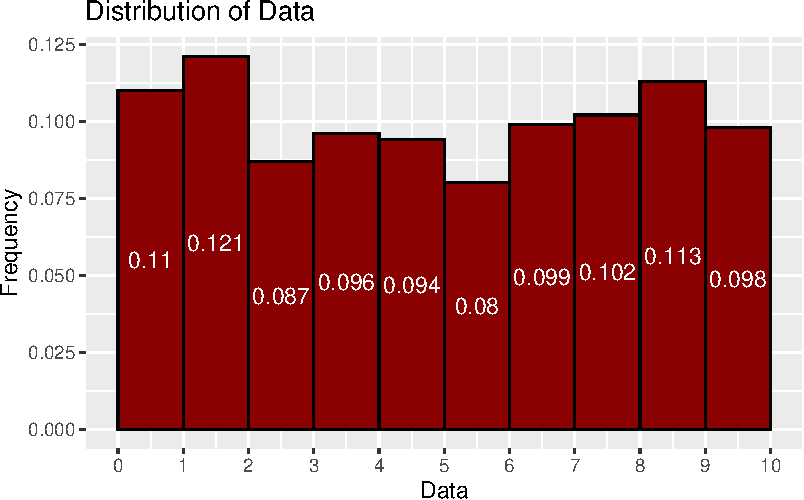
\includegraphics{Qualitative_and_Quantitative_Variables_files/figure-pdf/unnamed-chunk-4-1.pdf}

For continuous variables, it doesn't make since to have a histogram for
each individual values like we did for discrete variables. If we tried
this then we might need an \textbf{infinte} amount of bars or more!
Instead, we group the data into intervals (bins) of the same length and
then create a histogram based on these intervals. This is what we did
above. We grouped the data into intervals of 1 and then created a
histogram based on the intervals (0,1), (1, 2), (2, 3), etc. For this
histogram the bars represent the proportions (rounded to 3 decimal
places) of the data that fall into each interval. If you look at the
second bar in the histogram, you will see the number \texttt{0.121} in
the bar. This means that 12.1\% of the data falls into the interval (1,
2).

\begin{center}\rule{0.5\linewidth}{0.5pt}\end{center}

\section*{Exercises}\label{exercises}
\addcontentsline{toc}{section}{Exercises}

\markright{Exercises}

In this assignment, you will distinguish between different types of
variables: qualitative (nominal and ordinal) and quantitative (discrete
and continuous). Each question will present a variable, and you will
identify its type.

\subsection*{Problem 1}\label{problem-1}
\addcontentsline{toc}{subsection}{Problem 1}

\textbf{Gender identity of individuals in a survey.}

\begin{itemize}
\item
  \textbf{Type:}
\item
  \textbf{Explanation:}
\end{itemize}

\subsection*{Problem 2}\label{problem-2}
\addcontentsline{toc}{subsection}{Problem 2}

\textbf{Annual income of households in a city.}

\begin{itemize}
\item
  \textbf{Type:}
\item
  \textbf{Explanation:}
\end{itemize}

\subsection*{Problem 3}\label{problem-3}
\addcontentsline{toc}{subsection}{Problem 3}

\textbf{Number of books read by students in a year.}

\begin{itemize}
\item
  \textbf{Type:}
\item
  \textbf{Explanation:}
\end{itemize}

\subsection*{Problem 4}\label{problem-4}
\addcontentsline{toc}{subsection}{Problem 4}

\textbf{Educational attainment levels (e.g., high school diploma,
bachelor's degree, master's degree, etc.).}

\begin{itemize}
\item
  \textbf{Type:}
\item
  \textbf{Explanation:}
\end{itemize}

\subsection*{Problem 5}\label{problem-5}
\addcontentsline{toc}{subsection}{Problem 5}

\textbf{Number of reported hate crimes in different states.}

\begin{itemize}
\item
  \textbf{Type:}
\item
  \textbf{Explanation:}
\end{itemize}

\subsection*{Problem 6}\label{problem-6}
\addcontentsline{toc}{subsection}{Problem 6}

\textbf{Types of housing (e.g., owned, rented, homeless).}

\begin{itemize}
\item
  \textbf{Type:}
\item
  \textbf{Explanation:}
\end{itemize}

\subsection*{Problem 7}\label{problem-7}
\addcontentsline{toc}{subsection}{Problem 7}

\textbf{Age of participants in a community health study.}

\begin{itemize}
\item
  \textbf{Type:}
\item
  \textbf{Explanation:}
\end{itemize}

\subsection*{Problem 8}\label{problem-8}
\addcontentsline{toc}{subsection}{Problem 8}

\textbf{Political party affiliation (e.g., Democrat, Republican,
Independent).}

\begin{itemize}
\item
  \textbf{Type:}
\item
  \textbf{Explanation:}
\end{itemize}

\subsection*{Problem 9}\label{problem-9}
\addcontentsline{toc}{subsection}{Problem 9}

\textbf{Number of languages spoken by immigrants in a region.}

\begin{itemize}
\item
  \textbf{Type:}
\item
  \textbf{Explanation:}
\end{itemize}

\subsection*{Problem 10}\label{problem-10}
\addcontentsline{toc}{subsection}{Problem 10}

\textbf{Frequency of attending religious services (e.g., never,
occasionally, regularly).}

\begin{itemize}
\item
  \textbf{Type:}
\item
  \textbf{Explanation:}
\end{itemize}

\subsection*{Problem 11}\label{problem-11}
\addcontentsline{toc}{subsection}{Problem 11}

\textbf{Number of protests attended in a year.}

\begin{itemize}
\item
  \textbf{Type:}
\item
  \textbf{Explanation:}
\end{itemize}

\subsection*{Problem 12}\label{problem-12}
\addcontentsline{toc}{subsection}{Problem 12}

\textbf{Types of discrimination experienced (e.g., racial, gender,
disability).}

\begin{itemize}
\item
  \textbf{Type:}
\item
  \textbf{Explanation:}
\end{itemize}

\subsection*{Problem 13}\label{problem-13}
\addcontentsline{toc}{subsection}{Problem 13}

\textbf{Height of students in a classroom.}

\begin{itemize}
\item
  \textbf{Type:}
\item
  \textbf{Explanation:}
\end{itemize}

\subsection*{Problem 14}\label{problem-14}
\addcontentsline{toc}{subsection}{Problem 14}

\textbf{Marital status (e.g., single, married, divorced, widowed).}

\begin{itemize}
\item
  \textbf{Type:}
\item
  \textbf{Explanation:}
\end{itemize}

\subsection*{Problem 15}\label{problem-15}
\addcontentsline{toc}{subsection}{Problem 15}

\textbf{Number of social media accounts owned by individuals.}

\begin{itemize}
\item
  \textbf{Type:}
\item
  \textbf{Explanation:}
\end{itemize}

\subsection*{Problem 16}\label{problem-16}
\addcontentsline{toc}{subsection}{Problem 16}

\textbf{Severity of food insecurity (e.g., none, mild, moderate,
severe).}

\begin{itemize}
\item
  \textbf{Type:}
\item
  \textbf{Explanation:}
\end{itemize}

\subsection*{Problem 17}\label{problem-17}
\addcontentsline{toc}{subsection}{Problem 17}

\textbf{Number of children in a family.}

\begin{itemize}
\item
  \textbf{Type:}
\item
  \textbf{Explanation:}
\end{itemize}

\subsection*{Problem 18}\label{problem-18}
\addcontentsline{toc}{subsection}{Problem 18}

\textbf{Types of employment (e.g., full-time, part-time, unemployed).}

\begin{itemize}
\item
  \textbf{Type:}
\item
  \textbf{Explanation:}
\end{itemize}

\subsection*{Problem 19}\label{problem-19}
\addcontentsline{toc}{subsection}{Problem 19}

\textbf{Monthly electricity usage in kilowatt-hours.}

\begin{itemize}
\item
  \textbf{Type:}
\item
  \textbf{Explanation:}
\end{itemize}

\subsection*{Problem 20}\label{problem-20}
\addcontentsline{toc}{subsection}{Problem 20}

\textbf{Frequency of using public transportation (e.g., never,
sometimes, always).}

\begin{itemize}
\item
  \textbf{Type:}
\item
  \textbf{Explanation:}
\end{itemize}

\bookmarksetup{startatroot}

\chapter*{Intro to R}\label{intro-to-r}
\addcontentsline{toc}{chapter}{Intro to R}

\markboth{Intro to R}{Intro to R}

In this section we are going to go through some of the basics to
programming in R. We will look at how to comment your work, basic
calculator computations, create a variable, create a vector, how to
install a library / package, and use some of the built-in functions.

\section*{Comments}\label{comments}
\addcontentsline{toc}{section}{Comments}

\markright{Comments}

Comments are a very important part of coding. When you are writing code,
you will want to leave notes to yourself and your collaborators to
describe what you are doing at each step. You can also leave notes on
parts of the code that are norking or that you feel should be changed.
It is a way to remind yourself and your collaborators the work that has
been done, why it was done, what is broken, other changes you want to
make, and more. They are especially important when you come back to the
code after not having looked at it for a while.

Basically, leave as many comments as possible while coding. You should
start with the names of those that are working on the project with a
synopsis on what is the purpose of the project.

A comment is any text following a hashtag (\#) on the same line. This
text is ignored by the R compiler and does not affect how the script is
run. This is an example of how you should start every script you write
in this class or at your job.

\begin{Shaded}
\begin{Highlighting}[]
\CommentTok{\# Mike LeVan}
\CommentTok{\# Data{-}1004 Data Analytics and Statistics}
\CommentTok{\# Date}

\CommentTok{\# Assignment Description}

\CommentTok{\# I can write out notes to myself and my colleagues!}

\CommentTok{\# R ignores all the lines that start with \#}
\end{Highlighting}
\end{Shaded}

\section*{Calculator}\label{calculator}
\addcontentsline{toc}{section}{Calculator}

\markright{Calculator}

While this is quite a bit of overkill, R can be used as a basic
calculator. Here are the operators :

\subsection*{Addition ( + )}\label{addition}
\addcontentsline{toc}{subsection}{Addition ( + )}

\begin{Shaded}
\begin{Highlighting}[]
\CommentTok{\# This is an example of addition.}

\DecValTok{4} \SpecialCharTok{+} \DecValTok{8}
\end{Highlighting}
\end{Shaded}

\begin{verbatim}
[1] 12
\end{verbatim}

Notice the output above :

\texttt{{[}1{]}\ 12}

The {[}1{]} means the first output followed the by value of the output
12.

\subsection*{Subtraction ( - )}\label{subtraction--}
\addcontentsline{toc}{subsection}{Subtraction ( - )}

\begin{Shaded}
\begin{Highlighting}[]
\CommentTok{\# Here is an example of subtraction.}

\DecValTok{5} \SpecialCharTok{{-}} \DecValTok{14}
\end{Highlighting}
\end{Shaded}

\begin{verbatim}
[1] -9
\end{verbatim}

\subsection*{Multiplication ( * )}\label{multiplication}
\addcontentsline{toc}{subsection}{Multiplication ( * )}

\begin{Shaded}
\begin{Highlighting}[]
\CommentTok{\# Here is an example of multiplication}

\DecValTok{8} \SpecialCharTok{*} \DecValTok{17}
\end{Highlighting}
\end{Shaded}

\begin{verbatim}
[1] 136
\end{verbatim}

\subsection*{Division ( / )}\label{division}
\addcontentsline{toc}{subsection}{Division ( / )}

\begin{Shaded}
\begin{Highlighting}[]
\CommentTok{\# Division}

\DecValTok{22} \SpecialCharTok{/} \DecValTok{7}
\end{Highlighting}
\end{Shaded}

\begin{verbatim}
[1] 3.142857
\end{verbatim}

\subsection*{Exponentiation ( \^{} )}\label{exponentiation}
\addcontentsline{toc}{subsection}{Exponentiation ( \^{} )}

\begin{Shaded}
\begin{Highlighting}[]
\CommentTok{\# Exponentiation}

\DecValTok{5}\SpecialCharTok{\^{}}\DecValTok{3}
\end{Highlighting}
\end{Shaded}

\begin{verbatim}
[1] 125
\end{verbatim}

\subsection*{Square Roots and Radicals}\label{square-roots-and-radicals}
\addcontentsline{toc}{subsection}{Square Roots and Radicals}

Recall that we can use exponents to calculate radicals, too. If you
recall, the square root function is the same as raising a value to the
(1 / 2) power!

\begin{Shaded}
\begin{Highlighting}[]
\CommentTok{\# Here is the square root of 9}

\DecValTok{9}\SpecialCharTok{\^{}}\NormalTok{(}\DecValTok{1}\SpecialCharTok{/}\DecValTok{2}\NormalTok{)}
\end{Highlighting}
\end{Shaded}

\begin{verbatim}
[1] 3
\end{verbatim}

Notice that there are some levels of estimation / rounding here. For
example, calculate the square root of 2

\begin{Shaded}
\begin{Highlighting}[]
\DecValTok{2}\SpecialCharTok{\^{}}\NormalTok{(}\DecValTok{1}\SpecialCharTok{/}\DecValTok{2}\NormalTok{)}
\end{Highlighting}
\end{Shaded}

\begin{verbatim}
[1] 1.414214
\end{verbatim}

Obviously the real answer goes further than six decimal places. Also
think about the square root of 2 multiplied by itself. We should get the
value 2 right back :

\begin{Shaded}
\begin{Highlighting}[]
\DecValTok{2}\SpecialCharTok{\^{}}\NormalTok{(}\DecValTok{1}\SpecialCharTok{/}\DecValTok{2}\NormalTok{) }\SpecialCharTok{*} \DecValTok{2}\SpecialCharTok{\^{}}\NormalTok{(}\DecValTok{1}\SpecialCharTok{/}\DecValTok{2}\NormalTok{)}
\end{Highlighting}
\end{Shaded}

\begin{verbatim}
[1] 2
\end{verbatim}

But notice what happens if we then subtract 2 from the previous result :

\begin{Shaded}
\begin{Highlighting}[]
\DecValTok{2}\SpecialCharTok{\^{}}\NormalTok{(}\DecValTok{1}\SpecialCharTok{/}\DecValTok{2}\NormalTok{) }\SpecialCharTok{*} \DecValTok{2}\SpecialCharTok{\^{}}\NormalTok{(}\DecValTok{1}\SpecialCharTok{/}\DecValTok{2}\NormalTok{) }\SpecialCharTok{{-}} \DecValTok{2}
\end{Highlighting}
\end{Shaded}

\begin{verbatim}
[1] 4.440892e-16
\end{verbatim}

This result is in scientific notation, but what does it mean? When you
see the ``e-16'' part, that says to move the decimal places 16 spots to
the left, so this answer is closer to 0.000000000000000440892. Notice
that it is not zero, as it should be. This is because of the estimation
that was talked about above.

\subsection*{Creating a variable}\label{creating-a-variable}
\addcontentsline{toc}{subsection}{Creating a variable}

What is a variable? Imagine dumping some data in a bucket and then
giving that bucket a name. Now, every time you use that name, you are
really referring to what is in the bucket.

NOTE 1 : Recall our discussion from class about naming your variables.
You want to pick a name for your variables that make sense. It will make
editing your script much easier in the long run. If I called a variable
``Quiz\_Scores'' then we know what types of values we are working with.
If I called the variable ``x'' instead, what does that tell us about the
variable itself?

We can use an ``arrow'' to assign a value into a variable. An arrow is
just a less than sign followed by a dash with no spaces between them :

\texttt{\textless{}-}

For example, what if I wanted to assign the value 3 into a variable
called ``x'' and the value 7 into a variable called ``y'', we could type
this into our R script :

\begin{Shaded}
\begin{Highlighting}[]
\CommentTok{\# Assign 3 to the variable "x"}

\NormalTok{x }\OtherTok{\textless{}{-}} \DecValTok{3}

\CommentTok{\# Assign 7 to the variable "y"}

\NormalTok{y }\OtherTok{\textless{}{-}} \DecValTok{7}
\end{Highlighting}
\end{Shaded}

NOTE 2 : At this point you should look at the ENVIRONMENT window. This
window shows you the variables you are using and the values they
contain.

Now that we have values in these variables, we can now use them in our
script. For example, what if I wanted to perform some basic calculations
with these variables :

\subsection*{Addition of two variables : x +
y}\label{addition-of-two-variables-x-y}
\addcontentsline{toc}{subsection}{Addition of two variables : x + y}

\begin{Shaded}
\begin{Highlighting}[]
\CommentTok{\# We are going to calculate x + y. }

\CommentTok{\# Recall that x = 3 and y = 7 from above, so this should return 10}

\NormalTok{x }\SpecialCharTok{+}\NormalTok{ y}
\end{Highlighting}
\end{Shaded}

\begin{verbatim}
[1] 10
\end{verbatim}

We could do the same for several different operations :

\begin{Shaded}
\begin{Highlighting}[]
\CommentTok{\# Example 1 : Subtract two variables :}

\NormalTok{y }\SpecialCharTok{{-}}\NormalTok{ x}
\end{Highlighting}
\end{Shaded}

\begin{verbatim}
[1] 4
\end{verbatim}

\begin{Shaded}
\begin{Highlighting}[]
\CommentTok{\# Example 2 : Multiply a variable by a constant. We could multiply the variable x by 9 to}
\CommentTok{\# get 9 * 3 = 27}

\DecValTok{9}\SpecialCharTok{*}\NormalTok{x}
\end{Highlighting}
\end{Shaded}

\begin{verbatim}
[1] 27
\end{verbatim}

\begin{Shaded}
\begin{Highlighting}[]
\CommentTok{\# Example 3 : Take a linear combination of two different variables. For example, we can}
\CommentTok{\# multiply your by 2 and x by 3 and add them together to get }
\CommentTok{\# 2*7 + 3*3 = 13 + 9 = 23 }

\DecValTok{2}\SpecialCharTok{*}\NormalTok{y }\SpecialCharTok{+} \DecValTok{3}\SpecialCharTok{*}\NormalTok{x}
\end{Highlighting}
\end{Shaded}

\begin{verbatim}
[1] 23
\end{verbatim}

\begin{Shaded}
\begin{Highlighting}[]
\CommentTok{\# Example 4 : Use one variable as an exponent for another variable. In this case, take the }
\CommentTok{\# variable x and raise it to the power y. In this case, we are computing 3 \^{} 7}
\CommentTok{\# which is 3 * 3 * 3 * 3 * 3 * 3 * 3 = 2187:}

\NormalTok{x}\SpecialCharTok{\^{}}\NormalTok{y}
\end{Highlighting}
\end{Shaded}

\begin{verbatim}
[1] 2187
\end{verbatim}

\subsection*{Assigning Operations to
Variables}\label{assigning-operations-to-variables}
\addcontentsline{toc}{subsection}{Assigning Operations to Variables}

We could also take the result from an operation and assign that to a
different variable. For exampe, we could multiply x by 7 and multiply y
by 2, subtract them and store the result in a new variable z.

\begin{Shaded}
\begin{Highlighting}[]
\NormalTok{z }\OtherTok{\textless{}{-}} \DecValTok{7}\SpecialCharTok{*}\NormalTok{x }\SpecialCharTok{{-}} \DecValTok{2}\SpecialCharTok{*}\NormalTok{y}
\end{Highlighting}
\end{Shaded}

If you want to print out what is now in the variable z, you can now see
it in the ENVIRONMENT window. You can also type it out in the script :

\begin{Shaded}
\begin{Highlighting}[]
\CommentTok{\# Print out the variable z}

\NormalTok{z}
\end{Highlighting}
\end{Shaded}

\begin{verbatim}
[1] 7
\end{verbatim}

Recall from class that there are different kinds of variables we might
be asked to consider. We could have QUANTITATIVE data that could be in
the form of continuous or discrete values. Another kind of data we
talked about was CATEGORICAL data. Depending on the type of data you are
analyzing, you would need to perform different operations.

\subsection*{Creating vectors}\label{creating-vectors}
\addcontentsline{toc}{subsection}{Creating vectors}

Let's assume the class takes a quiz and I want to keep track of them.
Instead of creating a variable for each individual quiz, I can create
one vector that will have all of the scores.

For example, if I have the quiz scores 10, 5, 8, 9, 4 then I could
create the variables Student\_1\_Quiz, Student\_2\_Quiz, etc. It is much
easier to create a single variable that holds all of these values.

We will use the following command : \textbf{c( )}

The ``\textbf{c}'' is shorthand for ``\textbf{concatenate}'' which means
to link objects together in a chain or series.

If I wanted to create a vector for the quiz scores above, I would create
a vector called Quiz1\_Scores and assign the variables as follows :

Notice the order is important. If we want to assign the first student a
10, the second a 5, the third an 8, the fourth a 9, and the fifth a 4,
then we would do the following :

\begin{Shaded}
\begin{Highlighting}[]
\CommentTok{\# Create a vector and call it "Quiz1\_Scores" }

\NormalTok{Quiz1\_Scores }\OtherTok{\textless{}{-}} \FunctionTok{c}\NormalTok{(}\DecValTok{10}\NormalTok{, }\DecValTok{5}\NormalTok{, }\DecValTok{8}\NormalTok{, }\DecValTok{9}\NormalTok{ ,}\DecValTok{4}\NormalTok{)}
\end{Highlighting}
\end{Shaded}

Notice how this is represented in the ENVIRONMENT window :

\begin{Shaded}
\begin{Highlighting}[]
\CommentTok{\# We can print out the variable to check what it contains}

\NormalTok{Quiz1\_Scores     }
\end{Highlighting}
\end{Shaded}

\begin{verbatim}
[1] 10  5  8  9  4
\end{verbatim}

This tells us the scores are located in spots 1, 2, 3, 4, 5 in the
vector. In this vector, the values in the spots are then shown as the
values : 10 5 8 9 4

Let's say Student 3 comes to see us and ask about their quiz grade. We
can then access the individual value as follows :

\begin{Shaded}
\begin{Highlighting}[]
\NormalTok{Quiz1\_Scores[}\DecValTok{3}\NormalTok{]}
\end{Highlighting}
\end{Shaded}

\begin{verbatim}
[1] 8
\end{verbatim}

If we wanted the fifth value in the vector we could say :

\begin{Shaded}
\begin{Highlighting}[]
\NormalTok{Quiz1\_Scores[}\DecValTok{5}\NormalTok{]}
\end{Highlighting}
\end{Shaded}

\begin{verbatim}
[1] 4
\end{verbatim}

If we wanted to print out the 3rd, 4th, and 5th scores, we could say :

\begin{Shaded}
\begin{Highlighting}[]
\NormalTok{Quiz1\_Scores[}\DecValTok{3}\SpecialCharTok{:}\DecValTok{5}\NormalTok{]}
\end{Highlighting}
\end{Shaded}

\begin{verbatim}
[1] 8 9 4
\end{verbatim}

Obviously we would want to make sure we enter in the data in an
appropriate order because if I rearrange the order I get a completely
different vector :

\begin{Shaded}
\begin{Highlighting}[]
\NormalTok{Quiz1\_Scores\_B }\OtherTok{\textless{}{-}} \FunctionTok{c}\NormalTok{(}\DecValTok{5}\NormalTok{, }\DecValTok{10}\NormalTok{, }\DecValTok{4}\NormalTok{, }\DecValTok{9}\NormalTok{, }\DecValTok{8}\NormalTok{)}
\end{Highlighting}
\end{Shaded}

While I have the same scores, they are located in different spots of the
vectors and would assign different values to Student 1, Student 2, etc.

We could also use characters in our vectors. We would need to make sure
we use quotation marks so the compiler does not think we are using other
variables in our vector.

\begin{Shaded}
\begin{Highlighting}[]
\NormalTok{Students }\OtherTok{\textless{}{-}} \FunctionTok{c}\NormalTok{(}\StringTok{"Alice"}\NormalTok{, }\StringTok{"Bob"}\NormalTok{, }\StringTok{"Chad"}\NormalTok{, }\StringTok{"Debbie"}\NormalTok{, }\StringTok{"Eric"}\NormalTok{)}
\end{Highlighting}
\end{Shaded}

Check out what is now in the ENVIRONMENT window :

\begin{Shaded}
\begin{Highlighting}[]
\CommentTok{\# Print out the Students vector :}

\NormalTok{Students}
\end{Highlighting}
\end{Shaded}

\begin{verbatim}
[1] "Alice"  "Bob"    "Chad"   "Debbie" "Eric"  
\end{verbatim}

The only real difference from above is the we are using characters
instead of numeric values and that is identified because of the ``chr''
notation in the description.

We can look at the individual entries jsut as we did above. To look at
the fourth entry in the vector we would type :

\begin{Shaded}
\begin{Highlighting}[]
\NormalTok{Students[}\DecValTok{4}\NormalTok{]}
\end{Highlighting}
\end{Shaded}

\begin{verbatim}
[1] "Debbie"
\end{verbatim}

If you are given a variable or vector and want to know what type of
values it contains, you can use the ``class'' command to tell you. Here
are some examples to check entire vectors or individual locations in a
vector :

\begin{Shaded}
\begin{Highlighting}[]
\FunctionTok{class}\NormalTok{(Quiz1\_Scores)}
\end{Highlighting}
\end{Shaded}

\begin{verbatim}
[1] "numeric"
\end{verbatim}

\begin{Shaded}
\begin{Highlighting}[]
\FunctionTok{class}\NormalTok{(Quiz1\_Scores[}\DecValTok{2}\NormalTok{])}
\end{Highlighting}
\end{Shaded}

\begin{verbatim}
[1] "numeric"
\end{verbatim}

\begin{Shaded}
\begin{Highlighting}[]
\FunctionTok{class}\NormalTok{(Students)}
\end{Highlighting}
\end{Shaded}

\begin{verbatim}
[1] "character"
\end{verbatim}

\begin{Shaded}
\begin{Highlighting}[]
\FunctionTok{class}\NormalTok{(Students[}\DecValTok{1}\NormalTok{])}
\end{Highlighting}
\end{Shaded}

\begin{verbatim}
[1] "character"
\end{verbatim}

\begin{Shaded}
\begin{Highlighting}[]
\FunctionTok{class}\NormalTok{(Students)}
\end{Highlighting}
\end{Shaded}

\begin{verbatim}
[1] "character"
\end{verbatim}

What happens if we mix our variables and have numbers and characters in
the same vector?

Here is how one could be created :

\begin{Shaded}
\begin{Highlighting}[]
\NormalTok{blah }\OtherTok{\textless{}{-}} \FunctionTok{c}\NormalTok{(}\DecValTok{4}\NormalTok{, }\StringTok{"dffdg"}\NormalTok{, }\DecValTok{6}\NormalTok{, }\DecValTok{9}\NormalTok{, }\StringTok{"trte"}\NormalTok{)}
\end{Highlighting}
\end{Shaded}

How does R interpret these values?

\begin{Shaded}
\begin{Highlighting}[]
\FunctionTok{class}\NormalTok{(blah)}
\end{Highlighting}
\end{Shaded}

\begin{verbatim}
[1] "character"
\end{verbatim}

Notice that it considers EVERY entry in this vector to be a CHARACTER
even though we entered some as numbers. Be careful with this as it could
cause issues on how we work and interact with this vector.

\subsection*{Libraries and Packages}\label{libraries-and-packages}
\addcontentsline{toc}{subsection}{Libraries and Packages}

When we start up a session of R, there are some commands that are
already built into the program that we can use. For instance, we used
the basic mathematics operations above.

You will eventually want to do a deeper analysis of the data that needs
a command that is not already installed in your current session of R.
This is where the idea of Libraries or Packages comes into play.

If there is a command we want to use that is not currently loaded into
R, we can install the package that includes the command.

You can see what is loaded already by clicking on the PACKAGES tab.

You will see the packages that are loaded up as they will have a check
mark indicated they have been installed.

Let's say there was something in the ``\textbf{tcltk}'' library I wanted
to use. I could then click on the check box for ``\textbf{tcltk}'' and a
message should come up in the Console showing that the package was
installed.

\textbf{\textgreater{} library(tcltk, lib.loc =
``/opt/R/4.3.1/lib/R/library'')}

We could remove the package by unclicking on the check box. We get a
confirmation in the Console :

\textbf{\textgreater{} detach(``package:tcltk'', unload = TRUE)}

What happens if we need a package that is not included in the list.
There are hundreds of packages that people have developed to use in R.

For example, consider the \textbf{tidyverse} library. This is a library
that contains several commands that we will be using over the semester.

If we know we are going to be using a specific library in our R script,
then we should install it at the top of the script. We would enter in a
command such as : \textbf{install.packages(``tidyverse'')}

Once we do this, you will see several different commands that are now
available for us to use to analyze our data set.

If you look at the Packages tab, you will see several new packages that
we can add to use in the program.

\textbf{tidyverse} comes with several packages. If you click on the
tidyverse package, you will see several packages installed :

\textbf{\textgreater{} library(tidyverse)}

── Attaching core tidyverse packages ────────────────────── tidyverse
2.0.0 ──

✔ dplyr 1.1.2 ✔ readr 2.1.4

✔ forcats 1.0.0 ✔ stringr 1.5.0

✔ ggplot2 3.4.2 ✔ tibble 3.2.1

✔ lubridate 1.9.2 ✔ tidyr 1.3.0

✔ purrr 1.0.1\\

These packages are now loaded into R. Note that is we uncheck the
tidyverse package, these are still loaded into R. We can remove them by
unchecking their package. For example, if I uncheck the ggplot2 package
you will see the following message :

\texttt{\textgreater{}\ detach("package:ggplot2",\ unload\ =\ TRUE)}

When you are starting to become a programmer it might be tempting just
to load up EVERYTING, but that is not good practice. When these packages
are loaded up, they are taking up memory. This can lead to slower
computation times as well as lead to larger files being generated,
wasting space. Try to be efficient and load up what you need and avoid
bloat.

\subsection*{Functions}\label{functions}
\addcontentsline{toc}{subsection}{Functions}

There are two kinds of functions we are going to deal with in class -
the ones that are built into R and ones we create ourselves. This lesson
will only consider the functions that are built in.

A \textbf{FUNCTION} is a command that takes in some kind of data,
manipulates it, and returns a value. It has the following form :

\textbf{FUNCTION\_NAME( data )}

This will simply print out the result. Remember we could also assign the
result to a variable.

\textbf{result \textless- FUNCTION\_NAME ( data)}

For example, go back to the quiz grades we had listed earlier. What if I
wanted to calculated the average (mean) of the quiz scores? I could
enter the following :

\begin{Shaded}
\begin{Highlighting}[]
\FunctionTok{mean}\NormalTok{(Quiz1\_Scores)}
\end{Highlighting}
\end{Shaded}

\begin{verbatim}
[1] 7.2
\end{verbatim}

I could assign the result to a variable, such as :

\begin{Shaded}
\begin{Highlighting}[]
\CommentTok{\# Calculate the average and store the result in the variable }
\CommentTok{\# named "Quiz1\_Average"}

\NormalTok{Quiz1\_Average }\OtherTok{\textless{}{-}} \FunctionTok{mean}\NormalTok{(Quiz1\_Scores)}

\CommentTok{\# Print out the average}

\NormalTok{Quiz1\_Average}
\end{Highlighting}
\end{Shaded}

\begin{verbatim}
[1] 7.2
\end{verbatim}

There are several other built in functions. Here are a few :

\textbf{min( ), max( ), mean( ), median( ), sum( ), range( ), abs( )}

If we wanted the highest quiz grade, we could say :

\begin{Shaded}
\begin{Highlighting}[]
\CommentTok{\# Find the maximum value :}

\FunctionTok{max}\NormalTok{(Quiz1\_Scores)}
\end{Highlighting}
\end{Shaded}

\begin{verbatim}
[1] 10
\end{verbatim}

If I wanted to know how many values are in my vector, I could say :

\begin{Shaded}
\begin{Highlighting}[]
\CommentTok{\# Use the length function :}

\FunctionTok{length}\NormalTok{(Quiz1\_Scores)}
\end{Highlighting}
\end{Shaded}

\begin{verbatim}
[1] 5
\end{verbatim}

If I wanted to pick a random number from 1 - 100, I could type the
following

\begin{Shaded}
\begin{Highlighting}[]
\FunctionTok{sample}\NormalTok{(}\DecValTok{100}\NormalTok{,}\DecValTok{1}\NormalTok{)}
\end{Highlighting}
\end{Shaded}

\begin{verbatim}
[1] 25
\end{verbatim}

If I wanted to pick three random numbers (all different) from 1 - 100,
we could say this :

\begin{Shaded}
\begin{Highlighting}[]
\FunctionTok{sample}\NormalTok{(}\DecValTok{100}\NormalTok{,}\DecValTok{3}\NormalTok{)}
\end{Highlighting}
\end{Shaded}

\begin{verbatim}
[1] 35 74 48
\end{verbatim}

If I wanted to pick seven random numbers from 1 - 100 where we could
have (but not guarantee) duplicate values, I could say this :

\begin{Shaded}
\begin{Highlighting}[]
\FunctionTok{sample}\NormalTok{(}\DecValTok{100}\NormalTok{, }\DecValTok{7}\NormalTok{, }\AttributeTok{replace=}\ConstantTok{TRUE}\NormalTok{)}
\end{Highlighting}
\end{Shaded}

\begin{verbatim}
[1] 66  4 41 55 88 79 61
\end{verbatim}

To create a random vector for a range of values, we can use sample
function. We just need to pass the range and the sample size inside the
sample function.

For example, if we want to create a random sample of size 20 for a range
of values between 1 to 100 then we can use the command sample(1:100,20)
and if the sample size is larger than 100 then we can add replace=TRUE
as shown in the below examples.

\begin{Shaded}
\begin{Highlighting}[]
\CommentTok{\# Create random sample of 20 values from 1 {-} 100}

\NormalTok{x1 }\OtherTok{\textless{}{-}} \FunctionTok{sample}\NormalTok{(}\DecValTok{1}\SpecialCharTok{:}\DecValTok{100}\NormalTok{,}\DecValTok{20}\NormalTok{)}

\CommentTok{\# Print out the result}

\NormalTok{x1}
\end{Highlighting}
\end{Shaded}

\begin{verbatim}
 [1] 77 14  5  8 11 61 52 24 65 39 36 41 63 99 96 12 17 79 18 57
\end{verbatim}

\begin{Shaded}
\begin{Highlighting}[]
\CommentTok{\# Create a sample of 200 values from 1 {-} 100. Obviously there will be repeats!}

\NormalTok{x2 }\OtherTok{\textless{}{-}} \FunctionTok{sample}\NormalTok{(}\DecValTok{1}\SpecialCharTok{:}\DecValTok{100}\NormalTok{,}\DecValTok{200}\NormalTok{,}\AttributeTok{replace=}\ConstantTok{TRUE}\NormalTok{)}

\CommentTok{\# Print out the sample}

\NormalTok{x2}
\end{Highlighting}
\end{Shaded}

\begin{verbatim}
  [1]  32  39  26  96   9  19  40  27  91  78  34  30  55  93  23  37  70  19
 [19]  33  59  52  95  48  45  82   1  78   8  53  47  26  85  35  30  10  28
 [37]  77  37  87   9  80  38  53  39  87  59  63  93  59  11  38  95  77  18
 [55]  58   8  17  20  39  12  49  92  96  15   7  14  26  59  66  25  79  95
 [73]  49  96  43  72  31  73  95  63  78  76  90  18  10   8  88  94   1  28
 [91]   7  50  63  87  38  13  76  51  10  85   2  69  99  27  44  40  97  35
[109]   2  56  44  51  69  58  78  65  38  79  61  20  28  19  22  59  76  48
[127]  11  35  94  53  77  73  61  88  92   4  59  28  34  89  63   9  50   3
[145]   9  87  38  52  85  96  94  67  27  71  30  60  85   5  41  80  87  85
[163]  27  87  98  24  22  61   1  74  90  76   8  57  66  78  71  98  19  78
[181]  18  70  18   9  52  60  28 100  91  84  28  79  62  52  89   5  96  68
[199]  28  92
\end{verbatim}

There are far too many built in functions to list. You may have to use a
book or The Google to help you find an appropriate one to use.

Lastly, make sure that the data you enter into the function makes sense.
For example, what if I tried to find the average of the names of the
students we put into the vector ``Students''? Let's remind ourselves
what we have saved in this variable :

\begin{Shaded}
\begin{Highlighting}[]
\NormalTok{Students}
\end{Highlighting}
\end{Shaded}

\begin{verbatim}
[1] "Alice"  "Bob"    "Chad"   "Debbie" "Eric"  
\end{verbatim}

It shouldn't make any sense to try to find the average of these because
these variables are \textbf{characters} and not \textbf{numeric}. What
should happen if we try to take an average of characters instead of
numerical values? Check the output below to see!

\begin{Shaded}
\begin{Highlighting}[]
\FunctionTok{mean}\NormalTok{(Students)}
\end{Highlighting}
\end{Shaded}

\begin{verbatim}
Warning in mean.default(Students): argument is not numeric or logical:
returning NA
\end{verbatim}

\begin{verbatim}
[1] NA
\end{verbatim}

Yeah, this is R pretty much telling us we are not using the function
correctly.

\subsection*{Boolean (Logical)
Variables}\label{boolean-logical-variables}
\addcontentsline{toc}{subsection}{Boolean (Logical) Variables}

On a side note, when the error message tells us that a variable is not
\textbf{logical}, R is not saying that we are being illogical. Instead,
R is referring to another type of variable we might discuss later. These
are called \textbf{boolean} or \textbf{logical} variables and all that
means is that our variable takes on one of two values : TRUE or FALSE.

If I wanted to set the variable \textbf{f} to TRUE and the variable
\textbf{g} to FALSE, I could do the following :

\begin{Shaded}
\begin{Highlighting}[]
\NormalTok{f }\OtherTok{\textless{}{-}} \ConstantTok{TRUE}

\NormalTok{g }\OtherTok{\textless{}{-}} \ConstantTok{FALSE}
\end{Highlighting}
\end{Shaded}

We could then print these out to see the result :

\begin{Shaded}
\begin{Highlighting}[]
\CommentTok{\# Print out f}
\NormalTok{f}
\end{Highlighting}
\end{Shaded}

\begin{verbatim}
[1] TRUE
\end{verbatim}

\begin{Shaded}
\begin{Highlighting}[]
\CommentTok{\# Print out g}
\NormalTok{g}
\end{Highlighting}
\end{Shaded}

\begin{verbatim}
[1] FALSE
\end{verbatim}

\subsection*{Boolean (Logical)
Operators}\label{boolean-logical-operators}
\addcontentsline{toc}{subsection}{Boolean (Logical) Operators}

There are several operators that we can use to compare values. Here are
a few :

\begin{itemize}
\tightlist
\item
  AND : \&
\item
  OR : \textbar{}
\item
  NOT : !
\item
  EQUALS : ==
\item
  NOT EQUALS : !=
\end{itemize}

Lets create some variables to see how these work.

\begin{Shaded}
\begin{Highlighting}[]
\NormalTok{a }\OtherTok{\textless{}{-}} \ConstantTok{TRUE}

\NormalTok{b }\OtherTok{\textless{}{-}} \ConstantTok{FALSE}

\NormalTok{c }\OtherTok{\textless{}{-}} \ConstantTok{TRUE}

\NormalTok{d }\OtherTok{\textless{}{-}} \ConstantTok{FALSE}
\end{Highlighting}
\end{Shaded}

Now we can use these variables to see how these operators work.

\begin{Shaded}
\begin{Highlighting}[]
\CommentTok{\# The AND operator will return TRUE if both values are TRUE. If one or }
\CommentTok{\# both are FALSE, then it will return FALSE.}

\NormalTok{a }\SpecialCharTok{\&}\NormalTok{ b}
\end{Highlighting}
\end{Shaded}

\begin{verbatim}
[1] FALSE
\end{verbatim}

\begin{Shaded}
\begin{Highlighting}[]
\NormalTok{a}\SpecialCharTok{\&}\NormalTok{c}
\end{Highlighting}
\end{Shaded}

\begin{verbatim}
[1] TRUE
\end{verbatim}

\begin{Shaded}
\begin{Highlighting}[]
\NormalTok{a}\SpecialCharTok{\&}\NormalTok{d}
\end{Highlighting}
\end{Shaded}

\begin{verbatim}
[1] FALSE
\end{verbatim}

\begin{Shaded}
\begin{Highlighting}[]
\NormalTok{b}\SpecialCharTok{\&}\NormalTok{c}
\end{Highlighting}
\end{Shaded}

\begin{verbatim}
[1] FALSE
\end{verbatim}

\begin{Shaded}
\begin{Highlighting}[]
\NormalTok{b}\SpecialCharTok{\&}\NormalTok{d}
\end{Highlighting}
\end{Shaded}

\begin{verbatim}
[1] FALSE
\end{verbatim}

\begin{Shaded}
\begin{Highlighting}[]
\NormalTok{c}\SpecialCharTok{\&}\NormalTok{d}
\end{Highlighting}
\end{Shaded}

\begin{verbatim}
[1] FALSE
\end{verbatim}

\begin{Shaded}
\begin{Highlighting}[]
\CommentTok{\# The OR operator will return TRUE if one or both values are TRUE. If both}
\CommentTok{\# are FALSE, then it will return FALSE.}

\NormalTok{a}\SpecialCharTok{|}\NormalTok{b}
\end{Highlighting}
\end{Shaded}

\begin{verbatim}
[1] TRUE
\end{verbatim}

\begin{Shaded}
\begin{Highlighting}[]
\NormalTok{a}\SpecialCharTok{|}\NormalTok{c}
\end{Highlighting}
\end{Shaded}

\begin{verbatim}
[1] TRUE
\end{verbatim}

\begin{Shaded}
\begin{Highlighting}[]
\NormalTok{a}\SpecialCharTok{|}\NormalTok{d}
\end{Highlighting}
\end{Shaded}

\begin{verbatim}
[1] TRUE
\end{verbatim}

\begin{Shaded}
\begin{Highlighting}[]
\NormalTok{b}\SpecialCharTok{|}\NormalTok{c}
\end{Highlighting}
\end{Shaded}

\begin{verbatim}
[1] TRUE
\end{verbatim}

\begin{Shaded}
\begin{Highlighting}[]
\NormalTok{b}\SpecialCharTok{|}\NormalTok{d}
\end{Highlighting}
\end{Shaded}

\begin{verbatim}
[1] FALSE
\end{verbatim}

\begin{Shaded}
\begin{Highlighting}[]
\NormalTok{c}\SpecialCharTok{|}\NormalTok{d}
\end{Highlighting}
\end{Shaded}

\begin{verbatim}
[1] TRUE
\end{verbatim}

\begin{Shaded}
\begin{Highlighting}[]
\CommentTok{\# The NOT operator will return the opposite of the value. If the value is TRUE}
\CommentTok{\# then it will return FALSE. If the value is FALSE, then it will return TRUE.}

\SpecialCharTok{!}\NormalTok{a}
\end{Highlighting}
\end{Shaded}

\begin{verbatim}
[1] FALSE
\end{verbatim}

\begin{Shaded}
\begin{Highlighting}[]
\SpecialCharTok{!}\NormalTok{b}
\end{Highlighting}
\end{Shaded}

\begin{verbatim}
[1] TRUE
\end{verbatim}

\begin{Shaded}
\begin{Highlighting}[]
\CommentTok{\# The EQUALS operator will return TRUE if the values are the same. If the values}
\CommentTok{\# are different, then it will return FALSE.}

\NormalTok{a}\SpecialCharTok{==}\NormalTok{b}
\end{Highlighting}
\end{Shaded}

\begin{verbatim}
[1] FALSE
\end{verbatim}

\begin{Shaded}
\begin{Highlighting}[]
\NormalTok{a}\SpecialCharTok{==}\NormalTok{c}
\end{Highlighting}
\end{Shaded}

\begin{verbatim}
[1] TRUE
\end{verbatim}

\begin{Shaded}
\begin{Highlighting}[]
\CommentTok{\# The NOT EQUALS operator will return TRUE if the values are different. If the values}
\CommentTok{\# are the same, then it will return FALSE.}

\NormalTok{a}\SpecialCharTok{!=}\NormalTok{b}
\end{Highlighting}
\end{Shaded}

\begin{verbatim}
[1] TRUE
\end{verbatim}

\begin{Shaded}
\begin{Highlighting}[]
\NormalTok{a}\SpecialCharTok{!=}\NormalTok{c}
\end{Highlighting}
\end{Shaded}

\begin{verbatim}
[1] FALSE
\end{verbatim}

\begin{center}\rule{0.5\linewidth}{0.5pt}\end{center}

\section*{Exercises}\label{exercises-1}
\addcontentsline{toc}{section}{Exercises}

\markright{Exercises}

This exercise set will review the basic functions of R. Most of the
commands were reviewed in the lesson, but there are a few that you will
have to look up to see how to carry out the commands.

\textbf{Instructions}

\begin{itemize}
\tightlist
\item
  Write R code to solve each of the following problems.
\item
  Make sure to test your code to ensure it works correctly.
\item
  Provide comments in your code to explain your logic where necessary.
\end{itemize}

Problem 1: Addition

Add two numbers, 12 and 34.

\begin{Shaded}
\begin{Highlighting}[]
\CommentTok{\# Response}
\end{Highlighting}
\end{Shaded}

Problem 2: Subtraction

Subtract 25 from 75.

\begin{Shaded}
\begin{Highlighting}[]
\CommentTok{\# Response}
\end{Highlighting}
\end{Shaded}

Problem 3: Multiplication

Multiply 28 by 19.

\begin{Shaded}
\begin{Highlighting}[]
\CommentTok{\# Response}
\end{Highlighting}
\end{Shaded}

Problem 4: Division

Divide 144 by 12.

\begin{Shaded}
\begin{Highlighting}[]
\CommentTok{\# Response}
\end{Highlighting}
\end{Shaded}

Problem 5: Exponentiation

Calculate 9 raised to the power of 7.

\begin{Shaded}
\begin{Highlighting}[]
\CommentTok{\# Response}
\end{Highlighting}
\end{Shaded}

Problem 6: Square Root

Find the square root of 64.

\begin{Shaded}
\begin{Highlighting}[]
\CommentTok{\# Response}
\end{Highlighting}
\end{Shaded}

Problem 7: Logarithm

Calculate the natural logarithm (base e) of 20.

\begin{Shaded}
\begin{Highlighting}[]
\CommentTok{\# Response}
\end{Highlighting}
\end{Shaded}

Problem 8: Absolute Value

Find the absolute value of -15.

\begin{Shaded}
\begin{Highlighting}[]
\CommentTok{\# Response}
\end{Highlighting}
\end{Shaded}

Problem 9: Factorial

Calculate the factorial of 6.

\begin{Shaded}
\begin{Highlighting}[]
\CommentTok{\# Response}
\end{Highlighting}
\end{Shaded}

Problem 10: Variables

Create a variable \texttt{x} that is assigned the value 10 and another
variable \texttt{y} that is assigned the value 5. Add the two variables
together.

\begin{Shaded}
\begin{Highlighting}[]
\CommentTok{\# Response}
\end{Highlighting}
\end{Shaded}

Problem 11: Variables

Create a variable \texttt{z} that is the combination of
\texttt{11*x\ +\ 13*y}, where \texttt{x} and \texttt{y} are from the
previous problem.

\begin{Shaded}
\begin{Highlighting}[]
\CommentTok{\# Response}
\end{Highlighting}
\end{Shaded}

Problem 12: Mean and Median of a Vector

Find the mean and median of the elements in the vector c(2, 4, 6, 8, 10,
12, 14, 16, 18, 20).

\begin{Shaded}
\begin{Highlighting}[]
\CommentTok{\# Response}
\end{Highlighting}
\end{Shaded}

Problem 13: Create a Vector

Create a vector (with an appropriate name) that contains the names of 5
of your friends. What is the class of this vector?

\begin{Shaded}
\begin{Highlighting}[]
\CommentTok{\# Response}
\end{Highlighting}
\end{Shaded}

Problem 14:

Create a vector with 20 random values between 300 and 500. What is the
mean of this vector? What is the median of this vector?

\begin{Shaded}
\begin{Highlighting}[]
\CommentTok{\# Response}
\end{Highlighting}
\end{Shaded}

Problem 15: Maximum and Minimum

Find the maximum and minimum values of the vector created in Problem 14.

\begin{Shaded}
\begin{Highlighting}[]
\CommentTok{\# Response}
\end{Highlighting}
\end{Shaded}

Problem 16: Vectors

In the vector you created in problem 14 :

\begin{itemize}
\tightlist
\item
  Print out the 7th element.
\item
  Print out the first 10 elements.
\item
  Print out the last 5 elements.
\item
  Add the 4th and 18th elements together.
\end{itemize}

\begin{Shaded}
\begin{Highlighting}[]
\CommentTok{\# Response}
\end{Highlighting}
\end{Shaded}

Problem 17: Loading Libraries

Load the library \texttt{readr} and use the help file to find out what
the \texttt{read\_csv} function does.

\begin{Shaded}
\begin{Highlighting}[]
\CommentTok{\# Response}
\end{Highlighting}
\end{Shaded}

Problem 18: Boolean Vectors

Create a boolean vector that contains the values TRUE, FALSE, TRUE,
TRUE, FALSE. Print out the vector.

\begin{Shaded}
\begin{Highlighting}[]
\CommentTok{\# Response}
\end{Highlighting}
\end{Shaded}

Problem 19: Logical Operators

\begin{Shaded}
\begin{Highlighting}[]
\CommentTok{\# Explain the output for the following code :}

\NormalTok{x }\OtherTok{\textless{}{-}} \ConstantTok{TRUE}

\NormalTok{y }\OtherTok{\textless{}{-}} \ConstantTok{FALSE}

\NormalTok{z }\OtherTok{\textless{}{-}} \ConstantTok{TRUE}

\NormalTok{x }\SpecialCharTok{\&}\NormalTok{ (y }\SpecialCharTok{|}\NormalTok{ z)}
\end{Highlighting}
\end{Shaded}

\begin{verbatim}
[1] TRUE
\end{verbatim}

Problem 20: Logical Operators

\begin{Shaded}
\begin{Highlighting}[]
\CommentTok{\# Explain the output for the following code :}

\NormalTok{x }\OtherTok{\textless{}{-}} \DecValTok{5}

\NormalTok{y }\OtherTok{\textless{}{-}} \DecValTok{10}

\NormalTok{z }\OtherTok{\textless{}{-}} \DecValTok{15}

\NormalTok{x }\SpecialCharTok{\textgreater{}}\NormalTok{ y }\SpecialCharTok{\&}\NormalTok{ y }\SpecialCharTok{\textless{}}\NormalTok{ z}
\end{Highlighting}
\end{Shaded}

\begin{verbatim}
[1] FALSE
\end{verbatim}

Problem 21: Commenting

Go back and make sure your code is commented. Make sure you have a
comment at the top of the script that includes your name, the class, and
the date. Make sure you have comments throughout the script to explain
what is happening at each step.

\bookmarksetup{startatroot}

\chapter*{Reading and Interpreting
Tables}\label{reading-and-interpreting-tables}
\addcontentsline{toc}{chapter}{Reading and Interpreting Tables}

\markboth{Reading and Interpreting Tables}{Reading and Interpreting
Tables}

Descriptive statistics are the first pieces of information used to
understand and represent a dataset. Their goal, in essence, is to
describe the main features of numerical and categorical information with
simple summaries. These summaries can be presented with a single numeric
measure, using summary tables, or via graphical representation. Here, I
illustrate the most common forms of descriptive statistics for
categorical data but keep in mind there are numerous ways to describe
and illustrate key features of data.

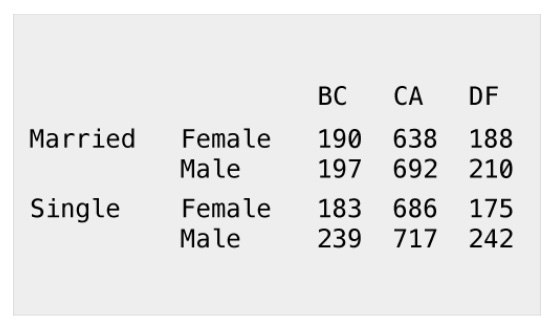
\includegraphics[width=0.35\textwidth,height=\textheight]{./images/Daily-6-Pic-1.jpg}

This tutorial covers the key features we are initially interested in
understanding for categorical data, to include:

\begin{itemize}
\tightlist
\item
  Frequencies: The number of observations for a particular category
\item
  Proportions: The percent that each category accounts for out of the
  whole
\item
  Marginals: The totals in a cross tabulation by row or column
\end{itemize}

\textbf{Replication Requirements}

To illustrate ways to compute these summary statistics and to visualize
categorical data, I'll demonstrate using this data which contains
artificial supermarket transaction data and can be found on our Canvas
page :

\textbf{Supermarket Transaction.xls}

Posit Cloud is running on a server, not your computer. To access a file
on your local drive, you need to upload it to the server. Click on the
Files tab (in the lower right pane) then on Upload. In the Upload Files
dialog, click on Choose File, navigate to the file and click on Open.
You can also change the target directory for the upload.

In addition, the packages we will need include the following:

\begin{Shaded}
\begin{Highlighting}[]
\CommentTok{\# install.packages("tidyverse")}
\FunctionTok{library}\NormalTok{(readxl)                   }\CommentTok{\# for reading in excel spreadsheet}
\end{Highlighting}
\end{Shaded}

First, let's read in the data. The data frame consists of 16 variables,
which I illustrate a select few below:

\begin{Shaded}
\begin{Highlighting}[]
\NormalTok{supermarket }\OtherTok{\textless{}{-}} \FunctionTok{read\_excel}\NormalTok{(}\StringTok{"./Supermarket Transactions.xlsx"}\NormalTok{)}

\CommentTok{\# Check out the first few lines but only columns 3,4,5,8,9,14,15,16}

\CommentTok{\# These are the 8 variables : Customer ID, Gender, Marital Status, Annual Income,}
\CommentTok{\# City, Product Category, Units Sold, Revenue}

\FunctionTok{head}\NormalTok{(supermarket[, }\FunctionTok{c}\NormalTok{(}\DecValTok{3}\SpecialCharTok{:}\DecValTok{5}\NormalTok{,}\DecValTok{8}\SpecialCharTok{:}\DecValTok{9}\NormalTok{,}\DecValTok{14}\SpecialCharTok{:}\DecValTok{16}\NormalTok{)])}
\end{Highlighting}
\end{Shaded}

\begin{verbatim}
# A tibble: 6 x 8
  `Customer ID` Gender `Marital Status` `Annual Income` City  `Product Category`
          <dbl> <chr>  <chr>            <chr>           <chr> <chr>             
1          7223 F      S                $30K - $50K     Los ~ Snack Foods       
2          7841 M      M                $70K - $90K     Los ~ Vegetables        
3          8374 F      M                $50K - $70K     Brem~ Snack Foods       
4          9619 M      M                $30K - $50K     Port~ Candy             
5          1900 F      S                $130K - $150K   Beve~ Carbonated Bevera~
6          6696 F      M                $10K - $30K     Beve~ Side Dishes       
# i 2 more variables: `Units Sold` <dbl>, Revenue <dbl>
\end{verbatim}

\textbf{Frequencies}

To produce \textbf{contingency tables} which calculate counts for each
combination of categorical variables we can use R's \textbf{table( )}
function. For instance, we may want to get the total count of female and
male customers.

\begin{Shaded}
\begin{Highlighting}[]
\FunctionTok{table}\NormalTok{(supermarket}\SpecialCharTok{$}\NormalTok{Gender)}
\end{Highlighting}
\end{Shaded}

\begin{verbatim}

   F    M 
7170 6889 
\end{verbatim}

If we want to understand the number of married and single females and
male customers we can produce a cross classification table:

\begin{Shaded}
\begin{Highlighting}[]
\CommentTok{\# cross classication counts for gender by marital status}

\FunctionTok{table}\NormalTok{(supermarket}\SpecialCharTok{$}\StringTok{\textasciigrave{}}\AttributeTok{Marital Status}\StringTok{\textasciigrave{}}\NormalTok{, supermarket}\SpecialCharTok{$}\NormalTok{Gender)}
\end{Highlighting}
\end{Shaded}

\begin{verbatim}
   
       F    M
  M 3602 3264
  S 3568 3625
\end{verbatim}

We can also produce multidimensional tables based on three or more
categorical variables. For this, we leverage the \textbf{ftable( )}
function to print the results more attractively. In this case we assess
the count of customers by marital status, gender, and location:

\begin{Shaded}
\begin{Highlighting}[]
\CommentTok{\# customer counts across location by gender and marital status}

\NormalTok{table1 }\OtherTok{\textless{}{-}} \FunctionTok{table}\NormalTok{(supermarket}\SpecialCharTok{$}\StringTok{\textasciigrave{}}\AttributeTok{Marital Status}\StringTok{\textasciigrave{}}\NormalTok{, supermarket}\SpecialCharTok{$}\NormalTok{Gender, supermarket}\SpecialCharTok{$}\StringTok{\textasciigrave{}}\AttributeTok{State or Province}\StringTok{\textasciigrave{}}\NormalTok{)}

\CommentTok{\# Remember that the previous command is taking the table we are creating and saving it into}
\CommentTok{\# a new variable called "table1". We will now take this table and evaluate it }
\CommentTok{\# using the **ftable( )** command.}

\FunctionTok{ftable}\NormalTok{(table1)}
\end{Highlighting}
\end{Shaded}

\begin{verbatim}
       BC   CA   DF Guerrero Jalisco   OR Veracruz   WA Yucatan Zacatecas
                                                                         
M F   190  638  188       77      15  510      142 1166     200       476
  M   197  692  210       94       5  514      108 1160     129       155
S F   183  686  175      107      30  607      125 1134     164       357
  M   239  717  242      105      25  631       89 1107     161       309
\end{verbatim}

\textbf{Proportions}

We can also produce contingency tables that present the proportions
(percentages) of each category or combination of categories. To do this
we simply feed the frequency tables produced by \textbf{table( )} to the
\textbf{prop.table( )} function. The following reproduces the previous
tables but calculates the proportions rather than counts:

\begin{Shaded}
\begin{Highlighting}[]
\CommentTok{\# Calculate the percentages of gender categories}

\CommentTok{\# We will first create a new table so we don\textquotesingle{}t accidentally hurt our previous work.}

\NormalTok{table2 }\OtherTok{\textless{}{-}} \FunctionTok{table}\NormalTok{(supermarket}\SpecialCharTok{$}\NormalTok{Gender)}

\CommentTok{\# After saving the output ( new table) to the variable table2, we will now send}
\CommentTok{\# this table2 to prop.table( ).}

\FunctionTok{prop.table}\NormalTok{(table2)}
\end{Highlighting}
\end{Shaded}

\begin{verbatim}

        F         M 
0.5099936 0.4900064 
\end{verbatim}

Based on the output, we can see that there are about 51\% of respondents
saying they are female (F) and about 49\% of the respondents saying they
are male (M).

We could also create a two-way table by adding another variable. For
example, let's create a table that tallies up the variables
\textbf{Marital Status} and \textbf{Gender}.

\begin{Shaded}
\begin{Highlighting}[]
\CommentTok{\# We shall create a new table (table3) to analyze. }

\NormalTok{table3 }\OtherTok{\textless{}{-}} \FunctionTok{table}\NormalTok{(supermarket}\SpecialCharTok{$}\StringTok{\textasciigrave{}}\AttributeTok{Marital Status}\StringTok{\textasciigrave{}}\NormalTok{, supermarket}\SpecialCharTok{$}\NormalTok{Gender)}

\CommentTok{\# We can now create a table of proportions for these variables.}

\FunctionTok{prop.table}\NormalTok{(table3)}
\end{Highlighting}
\end{Shaded}

\begin{verbatim}
   
            F         M
  M 0.2562060 0.2321644
  S 0.2537876 0.2578420
\end{verbatim}

We can interpret this tables as follows :

\begin{itemize}
\tightlist
\item
  25.6\% of the respondents identify as Female (F) and Married (M)
\item
  23.2\% of the respondents identify as Male (M) and Married (M)
\item
  25.3\% of the respondents identify as Female (F) and Single (S)
\item
  25.8\% of the respondents identify as Male (M) and Single (S)
\end{itemize}

Note that we can tell \textbf{ftable( )} how many decimal place to use
when reporting the results. For example, go back to table 1. We can
combine several commands together into one :

\begin{itemize}
\tightlist
\item
  We want to run \textbf{prop.table( )} on table 1
\item
  We want to limit to 3 decimal places
\item
  We want to round the results
\item
  We want to take this result and use \textbf{ftable( )}
\end{itemize}

\begin{Shaded}
\begin{Highlighting}[]
\FunctionTok{ftable}\NormalTok{(}\FunctionTok{round}\NormalTok{(}\FunctionTok{prop.table}\NormalTok{(table1), }\DecValTok{3}\NormalTok{))}
\end{Highlighting}
\end{Shaded}

\begin{verbatim}
        BC    CA    DF Guerrero Jalisco    OR Veracruz    WA Yucatan Zacatecas
                                                                              
M F  0.014 0.045 0.013    0.005   0.001 0.036    0.010 0.083   0.014     0.034
  M  0.014 0.049 0.015    0.007   0.000 0.037    0.008 0.083   0.009     0.011
S F  0.013 0.049 0.012    0.008   0.002 0.043    0.009 0.081   0.012     0.025
  M  0.017 0.051 0.017    0.007   0.002 0.045    0.006 0.079   0.011     0.022
\end{verbatim}

\textbf{Marginals}

Marginals show the total counts or percentages across columns or rows in
a contingency table. For instance, if we go back to table3 which is the
cross classification counts for gender by marital status:

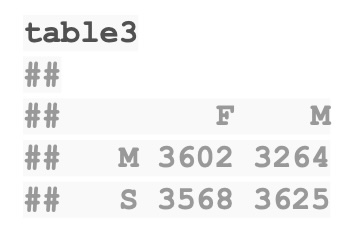
\includegraphics[width=0.2\textwidth,height=\textheight]{./images/Daily-6-Pic-2.jpg}

The \textbf{margins} are simply the sums of the rows and the columns.
For example, if we look at table3, I might want to know, ``How many
respondents identify as Single?'' This is the sum on the last row, 3568
+ 3625 = 7,193. Similarly, the amount of those identifying as Married
would be 3602 + 3264 = 6,866. We can calculate these values using the
\textbf{margin.table( )} command.

\begin{Shaded}
\begin{Highlighting}[]
\CommentTok{\# FREQUENCY MARGINALS}
\CommentTok{\# row marginals {-} totals for each marital status across gender}

\FunctionTok{margin.table}\NormalTok{(table3, }\DecValTok{1}\NormalTok{)}
\end{Highlighting}
\end{Shaded}

\begin{verbatim}

   M    S 
6866 7193 
\end{verbatim}

\begin{Shaded}
\begin{Highlighting}[]
\CommentTok{\# This command takes in the table for which we want to find the margins.}
\CommentTok{\# The second parameter tells us if we want row (1) or column (2) margins.}
\end{Highlighting}
\end{Shaded}

We can see that this example verifes the values we calculated above.

We could also calculate the column margins by changing the second
parameter to 2. It is left to you to verify that these values are
correct.

\begin{Shaded}
\begin{Highlighting}[]
\CommentTok{\# column marginals {-} totals for each gender across marital status}

\FunctionTok{margin.table}\NormalTok{(table3, }\DecValTok{2}\NormalTok{)}
\end{Highlighting}
\end{Shaded}

\begin{verbatim}

   F    M 
7170 6889 
\end{verbatim}

If we were more interested in proportions / percentage rather than
counts, we could use the \textbf{prop.table( )} command to calculate
these proportions. The first example will calculate the row percentages.

\begin{Shaded}
\begin{Highlighting}[]
\CommentTok{\# PERCENTAGE MARGINALS}

\CommentTok{\# row marginals {-} row percentages across gender}

\FunctionTok{prop.table}\NormalTok{(table3, }\AttributeTok{margin =} \DecValTok{1}\NormalTok{)}
\end{Highlighting}
\end{Shaded}

\begin{verbatim}
   
            F         M
  M 0.5246140 0.4753860
  S 0.4960378 0.5039622
\end{verbatim}

We could easily calcuate the column percentages using the following
command.

\begin{Shaded}
\begin{Highlighting}[]
\CommentTok{\# column marginals {-} column percentages across marital status}

\FunctionTok{prop.table}\NormalTok{(table3, }\AttributeTok{margin =} \DecValTok{2}\NormalTok{)}
\end{Highlighting}
\end{Shaded}

\begin{verbatim}
   
            F         M
  M 0.5023710 0.4737988
  S 0.4976290 0.5262012
\end{verbatim}

\begin{center}\rule{0.5\linewidth}{0.5pt}\end{center}

\section*{Exercises}\label{exercises-2}
\addcontentsline{toc}{section}{Exercises}

\markright{Exercises}

\begin{enumerate}
\def\labelenumi{\arabic{enumi}.}
\tightlist
\item
  Install and attch the library for the package \textbf{``vcd''}.
\end{enumerate}

\begin{Shaded}
\begin{Highlighting}[]
\CommentTok{\# Response}
\end{Highlighting}
\end{Shaded}

\begin{enumerate}
\def\labelenumi{\arabic{enumi}.}
\setcounter{enumi}{1}
\tightlist
\item
  Do a Google search to describe what we are getting when we load the
  \textbf{vcd} library.
\end{enumerate}

\begin{Shaded}
\begin{Highlighting}[]
\CommentTok{\# Put response in comments}
\end{Highlighting}
\end{Shaded}

\begin{enumerate}
\def\labelenumi{\arabic{enumi}.}
\setcounter{enumi}{2}
\tightlist
\item
  Describe what is in this data set (with \textbf{View(Arthritis)} ) and
  explain the variables and factors of each variable.
\end{enumerate}

\begin{Shaded}
\begin{Highlighting}[]
\CommentTok{\# Response}
\end{Highlighting}
\end{Shaded}

\begin{enumerate}
\def\labelenumi{\arabic{enumi}.}
\setcounter{enumi}{3}
\tightlist
\item
  Show what is in the 1st to the 17th rows of the frame ``Arthritis''
\end{enumerate}

\begin{Shaded}
\begin{Highlighting}[]
\CommentTok{\# Response}
\end{Highlighting}
\end{Shaded}

\begin{enumerate}
\def\labelenumi{\arabic{enumi}.}
\setcounter{enumi}{4}
\tightlist
\item
  Show rows 28 to 42 and only columns 2 and 5 of the frame ``Arthritis''
\end{enumerate}

\begin{Shaded}
\begin{Highlighting}[]
\CommentTok{\# Response}
\end{Highlighting}
\end{Shaded}

\begin{enumerate}
\def\labelenumi{\arabic{enumi}.}
\setcounter{enumi}{5}
\tightlist
\item
  Show patient ID's 1, 15, 42, and 81 and only the ``Treatment'' and
  ``Improved'' columns of the frame ``Arthritis'' using a single
  command.
\end{enumerate}

\begin{Shaded}
\begin{Highlighting}[]
\CommentTok{\# Response}
\end{Highlighting}
\end{Shaded}

\begin{enumerate}
\def\labelenumi{\arabic{enumi}.}
\setcounter{enumi}{6}
\tightlist
\item
  Show the summary information for ``Arthritis''
\end{enumerate}

\begin{Shaded}
\begin{Highlighting}[]
\CommentTok{\# Response}
\end{Highlighting}
\end{Shaded}

\begin{enumerate}
\def\labelenumi{\arabic{enumi}.}
\setcounter{enumi}{7}
\tightlist
\item
  Show the values of the ``Treatment'' column for ``Arthritis''
\end{enumerate}

\begin{Shaded}
\begin{Highlighting}[]
\CommentTok{\# Response}
\end{Highlighting}
\end{Shaded}

\begin{enumerate}
\def\labelenumi{\arabic{enumi}.}
\setcounter{enumi}{8}
\tightlist
\item
  Show the levels of the ``Treatment'' column for ``Arthritis''. (Hint :
  \textbf{levels} command\ldots..)
\end{enumerate}

\begin{Shaded}
\begin{Highlighting}[]
\CommentTok{\# Response}
\end{Highlighting}
\end{Shaded}

\begin{enumerate}
\def\labelenumi{\arabic{enumi}.}
\setcounter{enumi}{9}
\tightlist
\item
  Use the \textbf{length( )} function to find the number of patients in
  ``Arthritis''
\end{enumerate}

\begin{Shaded}
\begin{Highlighting}[]
\CommentTok{\# Response}
\end{Highlighting}
\end{Shaded}

\begin{enumerate}
\def\labelenumi{\arabic{enumi}.}
\setcounter{enumi}{10}
\tightlist
\item
  Use the \textbf{table( )} function to display the tabulated results
  for the ``Improved'' column of ``Arthritis'' (Note the
  \textbf{summary( )} function does the same thing). Put the result in
  the variable \textbf{``ImprovedTable''}.
\end{enumerate}

\begin{Shaded}
\begin{Highlighting}[]
\CommentTok{\# Response}
\end{Highlighting}
\end{Shaded}

\begin{enumerate}
\def\labelenumi{\arabic{enumi}.}
\setcounter{enumi}{11}
\tightlist
\item
  Use the \textbf{prop.table( )} function on \textbf{ImprovedTable} to
  get a table of proportions
\end{enumerate}

\begin{Shaded}
\begin{Highlighting}[]
\CommentTok{\# Response}
\end{Highlighting}
\end{Shaded}

\begin{enumerate}
\def\labelenumi{\arabic{enumi}.}
\setcounter{enumi}{12}
\tightlist
\item
  Use the \textbf{xtabs( )} function to cross-tabulate ``Treatment''
  versus ``Improved'' in the ``Arthritis'' data frame. Call the result
  \textbf{``Treat.Improv''}.
\end{enumerate}

\begin{Shaded}
\begin{Highlighting}[]
\CommentTok{\# Response}
\end{Highlighting}
\end{Shaded}

14. Add marginal sums to the table using the \textbf{addmargins( )}
function.

\begin{Shaded}
\begin{Highlighting}[]
\CommentTok{\# Response}
\end{Highlighting}
\end{Shaded}

15. Create 3 tables of proportions: proportion of \textbf{total},
proportion of \textbf{row sum}, and proportion of \textbf{column sum}.
Call the 3 tables: \textbf{P.Table1}, \textbf{P.Table2}, and
\textbf{P.Table3}

\begin{Shaded}
\begin{Highlighting}[]
\CommentTok{\# Response}
\end{Highlighting}
\end{Shaded}

\bookmarksetup{startatroot}

\chapter*{Barplots and Histograms}\label{barplots-and-histograms}
\addcontentsline{toc}{chapter}{Barplots and Histograms}

\markboth{Barplots and Histograms}{Barplots and Histograms}

Barplots (or Bar Charts) and Histograms are two of the most common ways
to visualize data, but they are often confused with one another.

A barplot is used to display the counts of unique values of a
categorical variable, while a histogram is used to display the
distribution of a continuous variable.

In this section, we will go over several examples of how to create
barplots and histograms in R. There are several techniques one could use
to create these plots, but we will focus on the \texttt{ggplot2} package
to create them.

\section*{Barplots}\label{barplots}
\addcontentsline{toc}{section}{Barplots}

\markright{Barplots}

Documentation for the bar chart / plot command can be found at the
following link:

bar plot / chart documentation

As we can see in the documentation :

There are two types of bar charts: \texttt{geom\_bar(\ )} and
\texttt{geom\_col(\ )}. \texttt{geom\_bar(\ )} makes the height of the
bar proportional to the number of cases in each group (or if the weight
aesthetic is supplied, the sum of the weights). If you want the heights
of the bars to represent values in the data, use \texttt{geom\_col(\ )}
instead.

You should read through this as it shows you all of the different
options you have when creating a barplot.

Let's revisit the data set we discussed in our previous Categorical
Variables section. Let's go back to the Supermarkets Transactions data
set to create a few barplots.

Let's first read in the data :

\begin{Shaded}
\begin{Highlighting}[]
\CommentTok{\# Read in the data}

\NormalTok{supermarket }\OtherTok{\textless{}{-}} \FunctionTok{read\_excel}\NormalTok{(}\StringTok{"./Supermarket Transactions.xlsx"}\NormalTok{)}

\CommentTok{\# Verify the data}

\FunctionTok{head}\NormalTok{(supermarket,}\DecValTok{2}\NormalTok{)}
\end{Highlighting}
\end{Shaded}

\begin{verbatim}
# A tibble: 2 x 16
  Transaction `Purchase Date`     `Customer ID` Gender `Marital Status`
        <dbl> <dttm>                      <dbl> <chr>  <chr>           
1           1 2011-12-18 00:00:00          7223 F      S               
2           2 2011-12-20 00:00:00          7841 M      M               
# i 11 more variables: Homeowner <chr>, Children <dbl>, `Annual Income` <chr>,
#   City <chr>, `State or Province` <chr>, Country <chr>,
#   `Product Family` <chr>, `Product Department` <chr>,
#   `Product Category` <chr>, `Units Sold` <dbl>, Revenue <dbl>
\end{verbatim}

In the previous section, we looked at a table that broke down the
customers by gender:

\begin{Shaded}
\begin{Highlighting}[]
\NormalTok{Table1 }\OtherTok{\textless{}{-}} \FunctionTok{table}\NormalTok{(supermarket}\SpecialCharTok{$}\NormalTok{Gender)}

\NormalTok{Table1}
\end{Highlighting}
\end{Shaded}

\begin{verbatim}

   F    M 
7170 6889 
\end{verbatim}

We can use ggplot to easily make a barplot of the Gender data. We will
create a barplot that has two bars, one for each gender listed in the
data set. Note that in the data set, the variable is listed with a
capitol letter. The variable we want to use is \textbf{Gender}, and not
gender. A small typo such as that can mess uo your entire code.

We will start off the \texttt{ggplot} command by telling the function
which data set we are using, and then we will use the \texttt{aes}
function to tell \texttt{ggplot} which variable we want to use for the
x-axis. We will then use the \texttt{geom\_bar} function to create the
barplot. Finally, we will use the \texttt{labs} function to add a title
to the plot, and to label the x and y axes.

\begin{Shaded}
\begin{Highlighting}[]
\FunctionTok{library}\NormalTok{(ggplot2)}

\CommentTok{\# here is how we can create a barplot of the count of  male and female gender from the supermarket data set}

\FunctionTok{ggplot}\NormalTok{(supermarket, }\FunctionTok{aes}\NormalTok{(}\AttributeTok{x =}\NormalTok{ Gender)) }\SpecialCharTok{+}
  \FunctionTok{geom\_bar}\NormalTok{() }\SpecialCharTok{+}
  \FunctionTok{labs}\NormalTok{(}\AttributeTok{title =} \StringTok{"Number of Shoppers by Gender"}\NormalTok{,}
       \AttributeTok{x =} \StringTok{"Gender"}\NormalTok{,}
       \AttributeTok{y =} \StringTok{"Count"}\NormalTok{)}
\end{Highlighting}
\end{Shaded}

\includegraphics{Barplots_And_Histograms_files/figure-pdf/unnamed-chunk-3-1.pdf}

If we wanted to make this look nicer, we could add some color to the
bars. The following example will change the color of the bars to
skyblue, and the outline of the bars to black. The \texttt{fill}
argument is used to change the color of the bars, and the \texttt{color}
argument is used to change the color of the outline of the bars.

\begin{Shaded}
\begin{Highlighting}[]
\FunctionTok{ggplot}\NormalTok{(supermarket, }\FunctionTok{aes}\NormalTok{(}\AttributeTok{x =}\NormalTok{ Gender)) }\SpecialCharTok{+}
  \FunctionTok{geom\_bar}\NormalTok{(}\AttributeTok{fill =} \StringTok{"skyblue"}\NormalTok{, }\AttributeTok{color =} \StringTok{"black"}\NormalTok{) }\SpecialCharTok{+}
  \FunctionTok{labs}\NormalTok{(}\AttributeTok{title =} \StringTok{"Number of People by Gender"}\NormalTok{,}
       \AttributeTok{x =} \StringTok{"Gender"}\NormalTok{,}
       \AttributeTok{y =} \StringTok{"Count"}\NormalTok{)}
\end{Highlighting}
\end{Shaded}

\includegraphics{Barplots_And_Histograms_files/figure-pdf/unnamed-chunk-4-1.pdf}

If we are feeling really fancy, we can have the bars with different
colors. We will add another layer using the \texttt{scale\_fill\_model}
function. This function will allow us to specify the colors we want to
use for each category. In this case, we will use pink for Females and
blue for Males. Al you need to do is create a vector that contains the
colors you wish to use.

We will also move the \texttt{fill} argument from the \texttt{geom\_bar}
function to the \texttt{aes} function. This will allow us to use the
\texttt{fill} argument in the \texttt{scale\_fill\_manual} function.

\begin{Shaded}
\begin{Highlighting}[]
\FunctionTok{ggplot}\NormalTok{(supermarket, }\FunctionTok{aes}\NormalTok{(}\AttributeTok{x =}\NormalTok{ Gender, }\AttributeTok{fill =}\NormalTok{ Gender)) }\SpecialCharTok{+}
  \FunctionTok{geom\_bar}\NormalTok{() }\SpecialCharTok{+}
  \FunctionTok{scale\_fill\_manual}\NormalTok{(}\AttributeTok{values =} \FunctionTok{c}\NormalTok{(}\StringTok{"F"} \OtherTok{=} \StringTok{"pink"}\NormalTok{, }\StringTok{"M"} \OtherTok{=} \StringTok{"blue"}\NormalTok{)) }\SpecialCharTok{+}
  \FunctionTok{labs}\NormalTok{(}\AttributeTok{title =} \StringTok{"Number of People by Gender"}\NormalTok{,}
       \AttributeTok{x =} \StringTok{"Gender"}\NormalTok{,}
       \AttributeTok{y =} \StringTok{"Count"}\NormalTok{)}
\end{Highlighting}
\end{Shaded}

\includegraphics{Barplots_And_Histograms_files/figure-pdf/unnamed-chunk-5-1.pdf}

We could also add the numbers of each count to the bars. This will help
the reader know the exact values from each category.

\begin{Shaded}
\begin{Highlighting}[]
\FunctionTok{ggplot}\NormalTok{(supermarket, }\FunctionTok{aes}\NormalTok{(}\AttributeTok{x =}\NormalTok{ Gender, }\AttributeTok{fill =}\NormalTok{ Gender)) }\SpecialCharTok{+}
  \FunctionTok{geom\_bar}\NormalTok{() }\SpecialCharTok{+}
  \FunctionTok{scale\_fill\_manual}\NormalTok{(}\AttributeTok{values =} \FunctionTok{c}\NormalTok{(}\StringTok{"F"} \OtherTok{=} \StringTok{"pink"}\NormalTok{, }\StringTok{"M"} \OtherTok{=} \StringTok{"blue"}\NormalTok{)) }\SpecialCharTok{+}
  \FunctionTok{geom\_text}\NormalTok{(}\AttributeTok{stat =} \StringTok{\textquotesingle{}count\textquotesingle{}}\NormalTok{, }\FunctionTok{aes}\NormalTok{(}\AttributeTok{label =} \FunctionTok{after\_stat}\NormalTok{(count)), }\AttributeTok{vjust =} \SpecialCharTok{{-}}\FloatTok{0.5}\NormalTok{) }\SpecialCharTok{+}
  \FunctionTok{labs}\NormalTok{(}\AttributeTok{title =} \StringTok{"Number of People by Gender"}\NormalTok{,}
       \AttributeTok{x =} \StringTok{"Gender"}\NormalTok{,}
       \AttributeTok{y =} \StringTok{"Count"}\NormalTok{)}
\end{Highlighting}
\end{Shaded}

\includegraphics{Barplots_And_Histograms_files/figure-pdf/unnamed-chunk-6-1.pdf}

\texttt{geom\_text(stat\ =\ \textquotesingle{}count\textquotesingle{},\ aes(label\ =\ ..count..),\ vjust\ =\ -0.5)}
is added to display the counts as text on each bar.

\texttt{stat\ =\ \textquotesingle{}count\textquotesingle{}} ensures that
the text is based on the count of each category.

\texttt{label\ =\ after\_stat(count)} specifies that the label should be
the count.

\texttt{vjust\ =\ -0.5} adjusts the vertical position of the text
slightly above the bar. Adjust this value as needed to position the text
correctly.

We could move the text to the middle of the bars, by playing around with
\texttt{vjust}. I found \texttt{vjust\ =\ 15} is a good value to center
the text on the bars in this case. It can change depending on your data
sets.

\begin{Shaded}
\begin{Highlighting}[]
\FunctionTok{ggplot}\NormalTok{(supermarket, }\FunctionTok{aes}\NormalTok{(}\AttributeTok{x =}\NormalTok{ Gender, }\AttributeTok{fill =}\NormalTok{ Gender)) }\SpecialCharTok{+}
  \FunctionTok{geom\_bar}\NormalTok{() }\SpecialCharTok{+}
  \FunctionTok{scale\_fill\_manual}\NormalTok{(}\AttributeTok{values =} \FunctionTok{c}\NormalTok{(}\StringTok{"F"} \OtherTok{=} \StringTok{"pink"}\NormalTok{, }\StringTok{"M"} \OtherTok{=} \StringTok{"blue"}\NormalTok{)) }\SpecialCharTok{+}
  \FunctionTok{geom\_text}\NormalTok{(}\AttributeTok{stat =} \StringTok{\textquotesingle{}count\textquotesingle{}}\NormalTok{, }\FunctionTok{aes}\NormalTok{(}\AttributeTok{label =} \FunctionTok{after\_stat}\NormalTok{(count)), }\AttributeTok{vjust =} \DecValTok{15}\NormalTok{, }\AttributeTok{color =} \StringTok{"white"}\NormalTok{) }\SpecialCharTok{+}
  \FunctionTok{labs}\NormalTok{(}\AttributeTok{title =} \StringTok{"Number of People by Gender"}\NormalTok{,}
       \AttributeTok{x =} \StringTok{"Gender"}\NormalTok{,}
       \AttributeTok{y =} \StringTok{"Count"}\NormalTok{)}
\end{Highlighting}
\end{Shaded}

\includegraphics{Barplots_And_Histograms_files/figure-pdf/unnamed-chunk-7-1.pdf}

We could also change the font size of the text. The following example
will change the font size to 5.

\begin{Shaded}
\begin{Highlighting}[]
\FunctionTok{ggplot}\NormalTok{(supermarket, }\FunctionTok{aes}\NormalTok{(}\AttributeTok{x =}\NormalTok{ Gender, }\AttributeTok{fill =}\NormalTok{ Gender)) }\SpecialCharTok{+}
  \FunctionTok{geom\_bar}\NormalTok{() }\SpecialCharTok{+}
  \FunctionTok{scale\_fill\_manual}\NormalTok{(}\AttributeTok{values =} \FunctionTok{c}\NormalTok{(}\StringTok{"F"} \OtherTok{=} \StringTok{"pink"}\NormalTok{, }\StringTok{"M"} \OtherTok{=} \StringTok{"blue"}\NormalTok{)) }\SpecialCharTok{+}
  \FunctionTok{geom\_text}\NormalTok{(}\AttributeTok{stat =} \StringTok{\textquotesingle{}count\textquotesingle{}}\NormalTok{, }\FunctionTok{aes}\NormalTok{(}\AttributeTok{label =} \FunctionTok{after\_stat}\NormalTok{(count)), }\AttributeTok{vjust =} \DecValTok{15}\NormalTok{, }\AttributeTok{color =} \StringTok{"white"}\NormalTok{, }\AttributeTok{size =} \DecValTok{5}\NormalTok{) }\SpecialCharTok{+}
  \FunctionTok{labs}\NormalTok{(}\AttributeTok{title =} \StringTok{"Number of People by Gender"}\NormalTok{,}
       \AttributeTok{x =} \StringTok{"Gender"}\NormalTok{,}
       \AttributeTok{y =} \StringTok{"Count"}\NormalTok{)}
\end{Highlighting}
\end{Shaded}

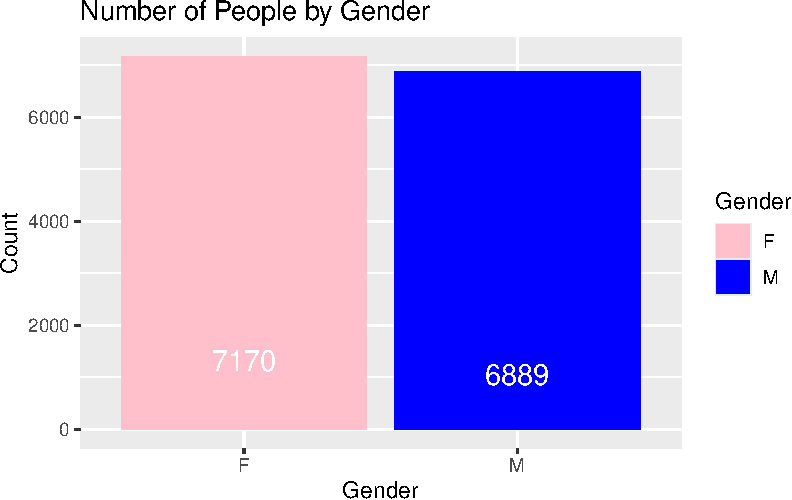
\includegraphics{Barplots_And_Histograms_files/figure-pdf/unnamed-chunk-8-1.pdf}

Consider the case to where we have more than two variables we want to
graph. For example, in the \texttt{Product\ Family} category, we have
three different factors : \textbf{Drink}, \textbf{Food}, and
\textbf{Non-Consumable}. We can create a barplot that shows the count of
each of these categories.

Notice that the \texttt{fill} argument tells \texttt{ggplot} which
variable to use for the color of the bars. We will use the
\texttt{scale\_fill\_manual} function to specify the colors we want to
use for each category.

\begin{Shaded}
\begin{Highlighting}[]
\FunctionTok{ggplot}\NormalTok{(supermarket, }\FunctionTok{aes}\NormalTok{(}\AttributeTok{x =} \StringTok{\textasciigrave{}}\AttributeTok{Product Family}\StringTok{\textasciigrave{}}\NormalTok{, }\AttributeTok{fill =} \StringTok{\textasciigrave{}}\AttributeTok{Product Family}\StringTok{\textasciigrave{}}\NormalTok{)) }\SpecialCharTok{+}
  \FunctionTok{geom\_bar}\NormalTok{() }\SpecialCharTok{+}
  \FunctionTok{scale\_fill\_manual}\NormalTok{(}\AttributeTok{values =} \FunctionTok{c}\NormalTok{(}\StringTok{"Food"} \OtherTok{=} \StringTok{"green"}\NormalTok{, }\StringTok{"Drink"} \OtherTok{=} \StringTok{"blue"}\NormalTok{, }\StringTok{"Non{-}Consumable"} \OtherTok{=} \StringTok{"red"}\NormalTok{)) }\SpecialCharTok{+}
  \FunctionTok{geom\_text}\NormalTok{(}\AttributeTok{stat =} \StringTok{\textquotesingle{}count\textquotesingle{}}\NormalTok{, }\FunctionTok{aes}\NormalTok{(}\AttributeTok{label =} \FunctionTok{after\_stat}\NormalTok{(count)), }\AttributeTok{vjust =} \DecValTok{2}\NormalTok{, }\AttributeTok{color =} \StringTok{"white"}\NormalTok{, }\AttributeTok{size =} \DecValTok{5}\NormalTok{) }\SpecialCharTok{+}
  \FunctionTok{labs}\NormalTok{(}\AttributeTok{title =} \StringTok{"Count of Product Family Categories"}\NormalTok{,}
       \AttributeTok{x =} \StringTok{"Product Family"}\NormalTok{,}
       \AttributeTok{y =} \StringTok{"Count"}\NormalTok{)}
\end{Highlighting}
\end{Shaded}

\includegraphics{Barplots_And_Histograms_files/figure-pdf/unnamed-chunk-9-1.pdf}

Lastly, we could create a barplot where the bars are stacked on top of
each other.

\begin{Shaded}
\begin{Highlighting}[]
\FunctionTok{ggplot}\NormalTok{(supermarket, }\FunctionTok{aes}\NormalTok{(}\AttributeTok{x =} \StringTok{""}\NormalTok{, }\AttributeTok{fill =} \StringTok{\textasciigrave{}}\AttributeTok{Product Family}\StringTok{\textasciigrave{}}\NormalTok{)) }\SpecialCharTok{+}
  \FunctionTok{geom\_bar}\NormalTok{() }\SpecialCharTok{+}
  \FunctionTok{scale\_fill\_manual}\NormalTok{(}\AttributeTok{values =} \FunctionTok{c}\NormalTok{(}\StringTok{"Food"} \OtherTok{=} \StringTok{"green"}\NormalTok{, }\StringTok{"Drink"} \OtherTok{=} \StringTok{"blue"}\NormalTok{, }\StringTok{"Non{-}Consumable"} \OtherTok{=} \StringTok{"red"}\NormalTok{)) }\SpecialCharTok{+}
  \FunctionTok{geom\_text}\NormalTok{(}\AttributeTok{stat =} \StringTok{\textquotesingle{}count\textquotesingle{}}\NormalTok{, }\FunctionTok{aes}\NormalTok{(}\AttributeTok{label =} \FunctionTok{after\_stat}\NormalTok{(count)), }\AttributeTok{position =} \FunctionTok{position\_stack}\NormalTok{(}\AttributeTok{vjust =} \FloatTok{0.5}\NormalTok{), }\AttributeTok{color =} \StringTok{"white"}\NormalTok{, }\AttributeTok{size =} \DecValTok{5}\NormalTok{) }\SpecialCharTok{+}
  \FunctionTok{labs}\NormalTok{(}\AttributeTok{title =} \StringTok{"Count of Product Family Categories"}\NormalTok{,}
       \AttributeTok{x =} \StringTok{"Product Family"}\NormalTok{,}
       \AttributeTok{y =} \StringTok{"Count"}\NormalTok{)}
\end{Highlighting}
\end{Shaded}

\includegraphics{Barplots_And_Histograms_files/figure-pdf/unnamed-chunk-10-1.pdf}

These can sometimes look better if drawn horizontally. We can do this by
flipping the axis using the \texttt{coord\_flip} function.

\begin{Shaded}
\begin{Highlighting}[]
\FunctionTok{ggplot}\NormalTok{(supermarket, }\FunctionTok{aes}\NormalTok{(}\AttributeTok{x =} \StringTok{""}\NormalTok{, }\AttributeTok{fill =} \StringTok{\textasciigrave{}}\AttributeTok{Product Family}\StringTok{\textasciigrave{}}\NormalTok{)) }\SpecialCharTok{+}
  \FunctionTok{geom\_bar}\NormalTok{() }\SpecialCharTok{+}
  \FunctionTok{scale\_fill\_manual}\NormalTok{(}\AttributeTok{values =} \FunctionTok{c}\NormalTok{(}\StringTok{"Food"} \OtherTok{=} \StringTok{"green"}\NormalTok{, }\StringTok{"Drink"} \OtherTok{=} \StringTok{"blue"}\NormalTok{, }\StringTok{"Non{-}Consumable"} \OtherTok{=} \StringTok{"red"}\NormalTok{)) }\SpecialCharTok{+}
  \FunctionTok{geom\_text}\NormalTok{(}\AttributeTok{stat =} \StringTok{\textquotesingle{}count\textquotesingle{}}\NormalTok{, }\FunctionTok{aes}\NormalTok{(}\AttributeTok{label =} \FunctionTok{after\_stat}\NormalTok{(count)), }\AttributeTok{position =} \FunctionTok{position\_stack}\NormalTok{(}\AttributeTok{vjust =} \FloatTok{0.5}\NormalTok{), }\AttributeTok{color =} \StringTok{"white"}\NormalTok{, }\AttributeTok{size =} \DecValTok{5}\NormalTok{) }\SpecialCharTok{+}
  \FunctionTok{labs}\NormalTok{(}\AttributeTok{title =} \StringTok{"Count of Product Family Categories"}\NormalTok{,}
       \AttributeTok{x =} \StringTok{"Product Family"}\NormalTok{,}
       \AttributeTok{y =} \StringTok{"Count"}\NormalTok{) }\SpecialCharTok{+}
  \FunctionTok{coord\_flip}\NormalTok{()}
\end{Highlighting}
\end{Shaded}

\includegraphics{Barplots_And_Histograms_files/figure-pdf/unnamed-chunk-11-1.pdf}

\section*{Histograms}\label{histograms}
\addcontentsline{toc}{section}{Histograms}

\markright{Histograms}

Histograms are used to display the distribution of a continuous
variable.

Documentation for the histogram command can be found at the following
link: histogram documentation

There are several arguments that can be used to customize the histogram
and you should review the documentation to see all of the options
available.

Let's create a histogram of the \textbf{Revenue} variable from the
supermarket data set. We will use the \texttt{geom\_histogram(\ )}
function to create the histogram. We will also use the \texttt{labs}
function to add a title to the plot, and to label the x and y axes.

The following is a basic default histogram before any customization:

\begin{Shaded}
\begin{Highlighting}[]
\FunctionTok{ggplot}\NormalTok{(supermarket, }\FunctionTok{aes}\NormalTok{(}\AttributeTok{x =} \StringTok{\textasciigrave{}}\AttributeTok{Revenue}\StringTok{\textasciigrave{}}\NormalTok{)) }\SpecialCharTok{+}
  \FunctionTok{geom\_histogram}\NormalTok{() }\SpecialCharTok{+}
  \FunctionTok{labs}\NormalTok{(}\AttributeTok{title =} \StringTok{"Revenue"}\NormalTok{,}
       \AttributeTok{x =} \StringTok{"Revenue"}\NormalTok{,}
       \AttributeTok{y =} \StringTok{"Count"}\NormalTok{)}
\end{Highlighting}
\end{Shaded}

\includegraphics{Barplots_And_Histograms_files/figure-pdf/unnamed-chunk-12-1.pdf}

We will see how we can customize this histogram. We will add color to
the bars, change the outline of the bars, and add a fill to the bars. We
will also add a title to the plot, and label the x and y axes.

However, one thing to note is that the \texttt{geom\_histogram} function
has a \texttt{binwidth} argument that can be used to change the width of
the bars. The default value is \texttt{binwidth\ =\ 30}. This means that
the bars will be 30 units wide. If we wanted to make the bars 10 units
wide, we would use \texttt{binwidth\ =\ 10}. If we wanted to make the
bars 5 units wide, we would use \texttt{binwidth\ =\ 5}. The smaller the
number, the more bars we will have. The larger the number, the fewer
bars we will have. A bad choice here could make the histogram look bad.
You will need to decide which value best represents your data.

\begin{Shaded}
\begin{Highlighting}[]
\FunctionTok{ggplot}\NormalTok{(supermarket, }\FunctionTok{aes}\NormalTok{(}\AttributeTok{x =} \StringTok{\textasciigrave{}}\AttributeTok{Revenue}\StringTok{\textasciigrave{}}\NormalTok{)) }\SpecialCharTok{+}
  \FunctionTok{geom\_histogram}\NormalTok{(}\AttributeTok{fill =} \StringTok{"skyblue"}\NormalTok{, }\AttributeTok{color =} \StringTok{"black"}\NormalTok{, }\AttributeTok{binwidth =} \DecValTok{30}\NormalTok{) }\SpecialCharTok{+}
  \FunctionTok{labs}\NormalTok{(}\AttributeTok{title =} \StringTok{"Revenue"}\NormalTok{,}
       \AttributeTok{x =} \StringTok{"Revenue"}\NormalTok{,}
       \AttributeTok{y =} \StringTok{"Count"}\NormalTok{)}
\end{Highlighting}
\end{Shaded}

\includegraphics{Barplots_And_Histograms_files/figure-pdf/unnamed-chunk-13-1.pdf}

This histogram has too few bars. This does not give us a good picture of
the distribution of the data. We can make a histogram where the bin
width is 5. Maybe this will give us a better picture of the distribution
of the data.

\begin{Shaded}
\begin{Highlighting}[]
\FunctionTok{ggplot}\NormalTok{(supermarket, }\FunctionTok{aes}\NormalTok{(}\AttributeTok{x =} \StringTok{\textasciigrave{}}\AttributeTok{Revenue}\StringTok{\textasciigrave{}}\NormalTok{)) }\SpecialCharTok{+}
  \FunctionTok{geom\_histogram}\NormalTok{(}\AttributeTok{fill =} \StringTok{"skyblue"}\NormalTok{, }\AttributeTok{color =} \StringTok{"black"}\NormalTok{, }\AttributeTok{binwidth =} \DecValTok{5}\NormalTok{) }\SpecialCharTok{+}
  \FunctionTok{labs}\NormalTok{(}\AttributeTok{title =} \StringTok{"Revenue"}\NormalTok{,}
       \AttributeTok{x =} \StringTok{"Revenue"}\NormalTok{,}
       \AttributeTok{y =} \StringTok{"Count"}\NormalTok{)}
\end{Highlighting}
\end{Shaded}

\includegraphics{Barplots_And_Histograms_files/figure-pdf/unnamed-chunk-14-1.pdf}

This is better. We can see that the data is skewed to the right. We can
also see that there are a few outliers. If we were doing some data
analysis, we could remove the outliers and see if the data is normally
distributed. We could also try to transform the data to see if it
becomes normally distributed. We will not do that here, but it is
something to consider when looking at data.

Also notice the locations of the bars. The bars are centered on the
x-axis values. This means that the bars are centered on the values 0, 5,
10, 15, 20, and so on. So the first bar has a width of 5 centered at 0.
This means the first bar starts at -2.5 and goes to 2.5. The second bar
starts at 2.5 and goes to 7.5. The third bar starts at 7.5 and goes to
12.5. And so on. This is not always the best way to display the data. If
we want the bars to start at 0 (or some other boundary) we can use the
\texttt{boundary} argument. The default value is
\texttt{boundary\ =\ 0}. This means that the bars will start at 0. If we
wanted the bars to start at 5, we would use \texttt{boundary\ =\ 5}. If
we wanted the bars to start at -5, we would use
\texttt{boundary\ =\ -5}.

\begin{Shaded}
\begin{Highlighting}[]
\FunctionTok{ggplot}\NormalTok{(supermarket, }\FunctionTok{aes}\NormalTok{(}\AttributeTok{x =} \StringTok{\textasciigrave{}}\AttributeTok{Revenue}\StringTok{\textasciigrave{}}\NormalTok{)) }\SpecialCharTok{+}
  \FunctionTok{geom\_histogram}\NormalTok{(}\AttributeTok{fill =} \StringTok{"skyblue"}\NormalTok{, }\AttributeTok{color =} \StringTok{"black"}\NormalTok{, }\AttributeTok{binwidth =} \DecValTok{5}\NormalTok{, }\AttributeTok{boundary=}\DecValTok{0}\NormalTok{) }\SpecialCharTok{+}
  \FunctionTok{labs}\NormalTok{(}\AttributeTok{title =} \StringTok{"Revenue"}\NormalTok{,}
       \AttributeTok{x =} \StringTok{"Revenue"}\NormalTok{,}
       \AttributeTok{y =} \StringTok{"Count"}\NormalTok{)}
\end{Highlighting}
\end{Shaded}

\includegraphics{Barplots_And_Histograms_files/figure-pdf/unnamed-chunk-15-1.pdf}

As we did with the baplot, we can add values to the histogram bars. This
is a tad tricky, and is not always the best way to display the data.
Many journals will include a table outlining the different intervals and
counts.

An additional layer that can be added to a histogram to help see the
distribution of the data is a density plot. The \texttt{geom\_density}
function can be used to add a density plot to the histogram. The density
plot will show the distribution of the data. The density plot is a
smoothed version of the histogram. The density plot is useful when the
data is not normally distributed. The density plot will show the
distribution of the data, and will show if the data is skewed to the
left or right, or if the data is bimodal.

The following example will add a density plot to the histogram. The
\texttt{geom\_density} function is used to add the density plot. The
\texttt{fill} argument is used to change the color of the density plot.
The \texttt{color} argument is used to change the outline of the density
plot. The \texttt{size} argument is used to change the size of the
density plot. The \texttt{alpha} argument is used to change the
transparency of the density plot. The \texttt{linetype} argument is used
to change the line type of the density plot. The \texttt{position}
argument is used to change the position of the density plot. The
\texttt{adjust} argument is used to change the adjustment of the density
plot.

The difficult part is that you will need to alter the \texttt{y} value
in the \texttt{aes} function to get the density plot to show up. The
\texttt{y} value is the height of the density plot. You will need to
play around with this value to get the density plot to show up. The
following example uses \texttt{y\ =\ after\_stat(density)*70000}.

\begin{Shaded}
\begin{Highlighting}[]
\FunctionTok{ggplot}\NormalTok{(supermarket, }\FunctionTok{aes}\NormalTok{(}\AttributeTok{x =} \StringTok{\textasciigrave{}}\AttributeTok{Revenue}\StringTok{\textasciigrave{}}\NormalTok{)) }\SpecialCharTok{+}
  \FunctionTok{geom\_histogram}\NormalTok{(}\AttributeTok{fill =} \StringTok{"skyblue"}\NormalTok{, }\AttributeTok{color =} \StringTok{"black"}\NormalTok{, }\AttributeTok{binwidth =} \DecValTok{5}\NormalTok{, }\AttributeTok{boundary=}\DecValTok{0}\NormalTok{) }\SpecialCharTok{+}
  \FunctionTok{geom\_density}\NormalTok{(}\FunctionTok{aes}\NormalTok{(}\AttributeTok{y=}\FunctionTok{after\_stat}\NormalTok{(density)}\SpecialCharTok{*}\DecValTok{70000}\NormalTok{), }\AttributeTok{fill =} \StringTok{"red"}\NormalTok{, }\AttributeTok{color =} \StringTok{"black"}\NormalTok{, }
               \AttributeTok{linewidth =} \DecValTok{1}\NormalTok{, }\AttributeTok{alpha =} \FloatTok{0.25}\NormalTok{, }\AttributeTok{linetype =} \StringTok{"dashed"}\NormalTok{, }
               \AttributeTok{position =} \StringTok{"stack"}\NormalTok{, }\AttributeTok{adjust =} \DecValTok{1}\NormalTok{) }\SpecialCharTok{+}
  \FunctionTok{labs}\NormalTok{(}\AttributeTok{title =} \StringTok{"Revenue"}\NormalTok{,}
       \AttributeTok{x =} \StringTok{"Revenue"}\NormalTok{,}
       \AttributeTok{y =} \StringTok{"Count"}\NormalTok{)}
\end{Highlighting}
\end{Shaded}

\includegraphics{Barplots_And_Histograms_files/figure-pdf/unnamed-chunk-16-1.pdf}

For more information on how to create nice histograms, you can read the
following :

https://www.appsilon.com/post/ggplot2-histograms

\begin{center}\rule{0.5\linewidth}{0.5pt}\end{center}

\section*{Exercises}\label{exercises-3}
\addcontentsline{toc}{section}{Exercises}

\markright{Exercises}

In this assignment, you will be working with a small dataset and using R
to create basic bar plots and histograms. This exercise will help you
get familiar with data visualization techniques, which are essential for
data analysis and interpretation.

\subsection*{Skills Checked}\label{skills-checked}
\addcontentsline{toc}{subsection}{Skills Checked}

\begin{enumerate}
\def\labelenumi{\arabic{enumi}.}
\tightlist
\item
  \textbf{Load the Dataset}: Load the provided dataset into R.
\item
  \textbf{Bar Plot}: Create a bar plot to visualize the data.
\item
  \textbf{Histogram}: Create a histogram to visualize the data.
\end{enumerate}

\subsection*{Barplot Dataset 1}\label{barplot-dataset-1}
\addcontentsline{toc}{subsection}{Barplot Dataset 1}

The following is a dataset that contains information about the number of
students enrolled in different courses at a university. Copy the
following dataset into a CSV file named \texttt{courses.csv} and upload
it to your working directory. Create an appropriate barchart depicting
the data.

\begin{longtable}[]{@{}lc@{}}
\toprule\noalign{}
Course & Number of Students \\
\midrule\noalign{}
\endhead
\bottomrule\noalign{}
\endlastfoot
Mathematics & 45 \\
Physics & 30 \\
Chemistry & 25 \\
Biology & 50 \\
Computer\_Science & 40 \\
History & 35 \\
English & 20 \\
Economics & 30 \\
\end{longtable}

\subsection*{Barplot Dataset 2}\label{barplot-dataset-2}
\addcontentsline{toc}{subsection}{Barplot Dataset 2}

The following is a dataset that contains sales information about the
number of electronic sales at your company. Copy the following dataset
into a CSV file named \texttt{sales.csv} and upload it to your working
directory. Create an appropriate barchart depicting the data.

\begin{longtable}[]{@{}lc@{}}
\toprule\noalign{}
Product & Sales \\
\midrule\noalign{}
\endhead
\bottomrule\noalign{}
\endlastfoot
Laptops & 120 \\
Smartphones & 200 \\
Tablets & 80 \\
Accessories & 150 \\
Wearables & 90 \\
Desktops & 70 \\
Cameras & 60 \\
Printers & 40 \\
\end{longtable}

\subsection*{Barplot Dataset 3}\label{barplot-dataset-3}
\addcontentsline{toc}{subsection}{Barplot Dataset 3}

The following is a dataset that contains monthly rainfall (in
millimeters) information for various cities across the United States.
Copy the following dataset into a CSV file named \texttt{rainfall}.csv`
and upload it to your working directory. Create an appropriate barchart
depicting the data.

\begin{longtable}[]{@{}lc@{}}
\toprule\noalign{}
City & Monthly\_Rainfall\_mm \\
\midrule\noalign{}
\endhead
\bottomrule\noalign{}
\endlastfoot
New\_York & 120 \\
Los\_Angeles & 20 \\
Chicago & 80 \\
Houston & 90 \\
Phoenix & 15 \\
Philadelphia & 100 \\
San\_Antonio & 70 \\
San\_Diego & 30 \\
Dallas & 85 \\
San\_Jose & 25 \\
\end{longtable}

\subsection*{Barplot Dataset 4}\label{barplot-dataset-4}
\addcontentsline{toc}{subsection}{Barplot Dataset 4}

The following is a dataset that contains monthly transatlantic
airtravel, in thousands of passengers, for 1958-1960. There are 4
fields, ``Month'', ``1958'', ``1959'' and ``1960'' and 12 records,
``JAN'' through ``DEC''.

Create a bar chart that shows the average number of passengers for each
month across the years 1958-1960.

Data :
https://people.sc.fsu.edu/\textasciitilde jburkardt/data/csv/airtravel.csv

You will need to downlaod the data set and load it into R.

\subsection*{Barplot Dataset 5}\label{barplot-dataset-5}
\addcontentsline{toc}{subsection}{Barplot Dataset 5}

Go to Kaggle and download the dat set ``US Christmas Tree Sales Data''
from the following link:

https://www.kaggle.com/datasets/thedevastator/us-christmas-tree-sales-data/data

Create a bar chart that shows the number of trees sold (per million) for
each year from 2010-2016.

\begin{Shaded}
\begin{Highlighting}[]
\NormalTok{tree\_data }\OtherTok{\textless{}{-}} \FunctionTok{read\_csv}\NormalTok{(}\StringTok{"./US\_Christmas\_Tree\_Sales\_2010\_to\_2016.csv"}\NormalTok{)}
\end{Highlighting}
\end{Shaded}

\subsection*{Histogram Dataset 1}\label{histogram-dataset-1}
\addcontentsline{toc}{subsection}{Histogram Dataset 1}

The following is a dataset (\texttt{Ages.csv}) that contains information
about the ages of participants at a local community center. Copy the
dataset into a CSV file named \texttt{ages\_data.csv} and upload it to
your working directory. Create a histogram with 7 bins depicting the
data.

\begin{Shaded}
\begin{Highlighting}[]
\NormalTok{ages\_data }\OtherTok{\textless{}{-}} \FunctionTok{read\_csv}\NormalTok{(}\StringTok{"./Ages.csv"}\NormalTok{)}

\NormalTok{ages\_data}
\end{Highlighting}
\end{Shaded}

\begin{verbatim}
# A tibble: 50 x 1
     Age
   <dbl>
 1    23
 2    27
 3    31
 4    35
 5    29
 6    42
 7    38
 8    45
 9    52
10    36
# i 40 more rows
\end{verbatim}

\subsection*{Histogram Dataset 2}\label{histogram-dataset-2}
\addcontentsline{toc}{subsection}{Histogram Dataset 2}

The following (\texttt{Lexington\_Temperature\_Data.csv}) is a dataset
that contains information about the daily temperature in Celsius for
Lexington the first 50 days of spring. Copy the dataset into a CSV file
named \texttt{Lex\_temps.csv} and upload it to your working directory.
Create a histogram with 4 bins depicting the data.

\begin{Shaded}
\begin{Highlighting}[]
\NormalTok{Lex\_temps }\OtherTok{\textless{}{-}} \FunctionTok{read\_csv}\NormalTok{(}\StringTok{"./Lexington\_Temperature\_Data.csv"}\NormalTok{)}

\NormalTok{Lex\_temps}
\end{Highlighting}
\end{Shaded}

\begin{verbatim}
# A tibble: 50 x 2
     Day Temperature
   <dbl>       <dbl>
 1     1        15.2
 2     2        16.5
 3     3        14.8
 4     4        17.1
 5     5        15.9
 6     6        16.2
 7     7        15  
 8     8        14.7
 9     9        16.8
10    10        15.4
# i 40 more rows
\end{verbatim}

\subsection*{Histogram Dataset 3}\label{histogram-dataset-3}
\addcontentsline{toc}{subsection}{Histogram Dataset 3}

The following is a data set
(\texttt{kentucky\_mens\_basketball\_wins.csv}) that contains
information about the number of wins for the University of Kentucky's
men's basketball team from 1980 - 2024. Copy the dataset into a CSV file
named \texttt{UK\_wins} and upload it to your working directory. Create
a histogram with 10 bins depicting the data on the amount of wins per
year.

\begin{Shaded}
\begin{Highlighting}[]
\NormalTok{UK\_wins }\OtherTok{\textless{}{-}} \FunctionTok{read\_csv}\NormalTok{(}\StringTok{"./kentucky\_mens\_basketball\_wins.csv"}\NormalTok{)}

\NormalTok{UK\_wins}
\end{Highlighting}
\end{Shaded}

\begin{verbatim}
# A tibble: 45 x 2
    Year Games_Won
   <dbl>     <dbl>
 1  1980        29
 2  1981        22
 3  1982        22
 4  1983        13
 5  1984        29
 6  1985        18
 7  1986        32
 8  1987        18
 9  1988        27
10  1989        13
# i 35 more rows
\end{verbatim}

\subsection*{Histogram Dataset 4}\label{histogram-dataset-4}
\addcontentsline{toc}{subsection}{Histogram Dataset 4}

The following is a data set
(\texttt{Fire\_Arm\_Deaths\_1990\_to\_2022.xlsx}) that contains
information about the number of firearm deaths in the US from 1990 -
2024. Copy the dataset into a CSV file named \texttt{Fire\_Arm\_Deaths}
and upload it to your working directory. Create a histogram with 10 bins
depicting the data on the amount of deaths per year.

\begin{Shaded}
\begin{Highlighting}[]
\FunctionTok{library}\NormalTok{(readxl)}

\NormalTok{Fire\_Arm\_Deaths }\OtherTok{\textless{}{-}} \FunctionTok{read\_csv}\NormalTok{(}\StringTok{"./Fire\_Arm\_Deaths\_1990\_to\_2022.csv"}\NormalTok{)}

\NormalTok{Fire\_Arm\_Deaths}
\end{Highlighting}
\end{Shaded}

\begin{verbatim}
# A tibble: 33 x 2
    Year Deaths
   <dbl>  <dbl>
 1  2022  48204
 2  2021  48830
 3  2020  45222
 4  2019  39707
 5  2018  39740
 6  2017  39773
 7  2016  38658
 8  2015  36252
 9  2014  33594
10  2013  33636
# i 23 more rows
\end{verbatim}

\subsection*{Histogram Dataset 5}\label{histogram-dataset-5}
\addcontentsline{toc}{subsection}{Histogram Dataset 5}

The data set (\texttt{gdp-per-capita-us-dollars-2020.csv}) contains
information about the GDP per capita in US dollars for various countries
in 2020. Download the data set from here and save it to yourworking
directory. Copy the dataset into a variable named
\texttt{gdp\_per\_capita}.

\begin{Shaded}
\begin{Highlighting}[]
\NormalTok{gdp\_per\_capita }\OtherTok{\textless{}{-}} \FunctionTok{read\_csv}\NormalTok{(}\StringTok{"./gdp{-}per{-}capita{-}us{-}dollars{-}2020.csv"}\NormalTok{)}

\FunctionTok{head}\NormalTok{(gdp\_per\_capita)}
\end{Highlighting}
\end{Shaded}

\begin{verbatim}
# A tibble: 6 x 2
  `Country Name`       `GDP Per Capita (Current US $ , 2020)`
  <chr>                                                 <dbl>
1 Afghanistan                                             517
2 Angola                                                 1776
3 Albania                                                5246
4 Algeria                                                3307
5 United Arab Emirates                                  36285
6 Argentina                                              8579
\end{verbatim}

\begin{itemize}
\tightlist
\item
  Create a histogram, with equal class widths, with the first class
  being (0 , 10000 {]} and covers all data values.
\item
  Create a histogram, with equal class widths, with the first class
  being (0 , 5000{]} with the last class being (55000 , 60000{]}
\item
  Create a histogram, with equal class widths, with the first class
  being (0 , 1000{]} with the last class being (19000 , 20000{]}
\item
  Compare all three histograms. Which one gives more information as to
  how the countries with low GDP are distributed?
\end{itemize}

\bookmarksetup{startatroot}

\chapter*{Line Graphs and Pie Charts}\label{line-graphs-and-pie-charts}
\addcontentsline{toc}{chapter}{Line Graphs and Pie Charts}

\markboth{Line Graphs and Pie Charts}{Line Graphs and Pie Charts}

Line graphs and pie charts are two of the most common ways to visualize
data. You can often find them in newspapers, magazines, and websites.

Line graphs are most useful when you want to show how data changes over
time. For example, you might use a line graph to show how a company's
stock price has changed over the past year.

Pie charts are also handy. They are best used when you want to show how
a whole is divided into parts. As an example, you might use a pie chart
to show how a company's revenue is divided among different products.

In this tutorial, we will learn how to create line graphs and pie charts
in R.

\section*{Line Graphs}\label{line-graphs}
\addcontentsline{toc}{section}{Line Graphs}

\markright{Line Graphs}

A line graph (or line chart) is used to display data points connected by
a continuous line. As we mentioned above, is especially useful for
showing trends over time.

What Does a Line Graph Do?

\begin{itemize}
\tightlist
\item
  Shows trends and patterns : It helps visualize how a variable changes
  over time (e.g., stock prices, temperature changes, sales growth).
\item
  Compares multiple data series : You can plot multiple lines to compare
  different categories or groups.
\item
  Identifies peaks and dips : It makes it easy to see the highest and
  lowest values in a dataset.
\item
  Helps in forecasting : By analyzing past trends, a line graph can give
  insights into possible future patterns.
\end{itemize}

When to Use a Line Graph?

\begin{itemize}
\tightlist
\item
  When data is continuous (e.g., time-based data like months, years, or
  days).
\item
  When you want to track changes over time.
\item
  When comparing trends across different categories.
\end{itemize}

In order to make a line graph in R, you need to make sure the following
libraries are loaded up :

\begin{itemize}
\tightlist
\item
  \texttt{dplyr}
\item
  \texttt{ggplot2}
\end{itemize}

We will use a combination of \texttt{ggplot(\ )} and the geometry
function \texttt{geom\_line(\ )} to create a line graph. the
\texttt{geom\_line(\ )} function connects the data points in the order
of the x-axis variable.

\subsection*{Unemployment Rate Example}\label{unemployment-rate-example}
\addcontentsline{toc}{subsection}{Unemployment Rate Example}

Let's take a look at an example of a line graph that shows the
unemployment rate over time using the built-in \texttt{economics}
dataset in R.

\begin{Shaded}
\begin{Highlighting}[]
\CommentTok{\# Load necessary libraries}
\FunctionTok{library}\NormalTok{(ggplot2)}
\FunctionTok{library}\NormalTok{(dplyr)}

\CommentTok{\# Load built{-}in economics dataset}

\FunctionTok{data}\NormalTok{(}\StringTok{"economics"}\NormalTok{)}

\CommentTok{\# Create a time series line plot of unemployment rate}

\NormalTok{economics }\SpecialCharTok{\%\textgreater{}\%}
  \FunctionTok{ggplot}\NormalTok{(}\FunctionTok{aes}\NormalTok{(}\AttributeTok{x =}\NormalTok{ date, }\AttributeTok{y =}\NormalTok{ unemploy)) }\SpecialCharTok{+}
  \FunctionTok{geom\_line}\NormalTok{(}\AttributeTok{color =} \StringTok{"blue"}\NormalTok{) }\SpecialCharTok{+}
  \FunctionTok{labs}\NormalTok{(}\AttributeTok{title =} \StringTok{"Unemployment Over Time"}\NormalTok{,}
       \AttributeTok{x =} \StringTok{"Year"}\NormalTok{,}
       \AttributeTok{y =} \StringTok{"Unemployment (in thousands)"}\NormalTok{) }\SpecialCharTok{+}
  \FunctionTok{theme\_minimal}\NormalTok{()}
\end{Highlighting}
\end{Shaded}

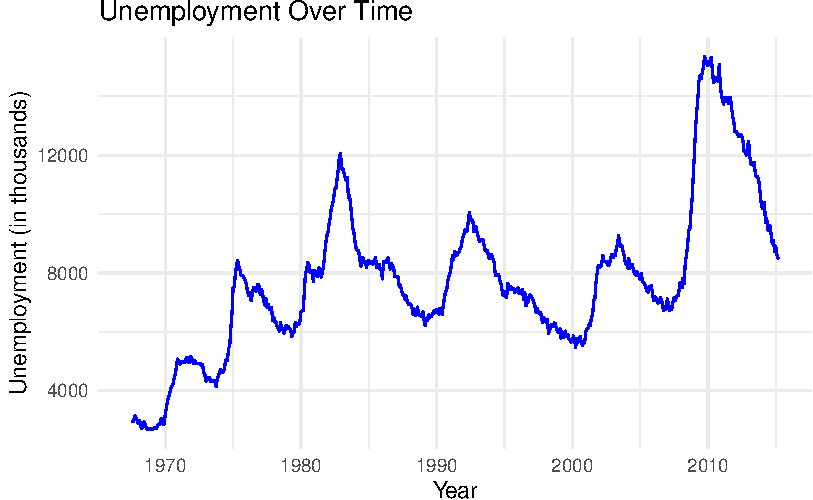
\includegraphics{Line_Graphs_and_Pie_Charts_files/figure-pdf/unnamed-chunk-1-1.pdf}

This graph shows the unemployment rate over time. We can see that the
rate fluctuates over time, with some periods of high unemployment and
some periods of low unemployment. This graph can help us understand how
the unemployment rate has changed over time and identify any trends or
patterns.

While line graphs are generally used as a way to show trends over time,
they can also be used to compare multiple data series. Let's look at an
example of a line graph that compares the price of a diamond to the size
(carat) of the diamond.

\subsection*{Diamond Price vs Carat Size
Example}\label{diamond-price-vs-carat-size-example}
\addcontentsline{toc}{subsection}{Diamond Price vs Carat Size Example}

Let's consider the \texttt{diamonds} dataset that comes with the
\texttt{ggplot2} package. This dataset contains information about the
price, carat, and cut of diamonds. We will use this dataset to create a
line graph that shows the comparison of average price versus carat size.

\begin{Shaded}
\begin{Highlighting}[]
\CommentTok{\# Load the libraries}

\FunctionTok{library}\NormalTok{(dplyr)}
\FunctionTok{library}\NormalTok{(ggplot2)}

\CommentTok{\# Create a line graph of the average price of diamonds over time}
\CommentTok{\# Aggregate data: Get the average price for each carat size}

\NormalTok{avg\_price\_per\_carat }\OtherTok{\textless{}{-}} \FunctionTok{aggregate}\NormalTok{(price }\SpecialCharTok{\textasciitilde{}}\NormalTok{ carat, }\AttributeTok{data =}\NormalTok{ diamonds, }\AttributeTok{FUN =}\NormalTok{ mean)}

\CommentTok{\# Create the line graph}
\FunctionTok{ggplot}\NormalTok{(avg\_price\_per\_carat, }\FunctionTok{aes}\NormalTok{(}\AttributeTok{x =}\NormalTok{ carat, }\AttributeTok{y =}\NormalTok{ price)) }\SpecialCharTok{+}
  \FunctionTok{geom\_line}\NormalTok{(}\AttributeTok{color =} \StringTok{"blue"}\NormalTok{, }\AttributeTok{linewidth =} \DecValTok{1}\NormalTok{) }\SpecialCharTok{+} 
  \FunctionTok{labs}\NormalTok{(}\AttributeTok{title =} \StringTok{"Diamond Price vs. Carat Size"}\NormalTok{,}
       \AttributeTok{x =} \StringTok{"Carat Size"}\NormalTok{,}
       \AttributeTok{y =} \StringTok{"Average Price (USD)"}\NormalTok{) }\SpecialCharTok{+}
  \FunctionTok{theme\_minimal}\NormalTok{()}
\end{Highlighting}
\end{Shaded}

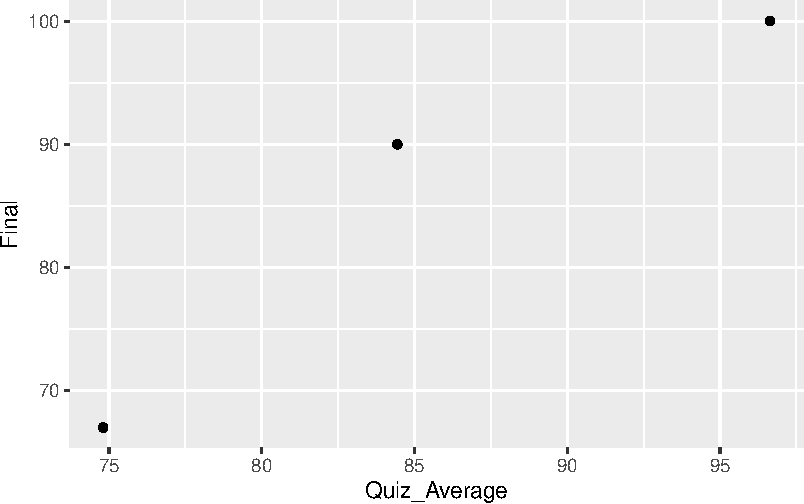
\includegraphics{Line_Graphs_and_Pie_Charts_files/figure-pdf/unnamed-chunk-2-1.pdf}

While certainly not a surprise, we can interpret from this graph that as
the number of carats in the diamond increases, the price of the diamond
also increases. It is curious as to why there is a dip in the price of
diamonds of size around 3 carats. This could be due to a variety of
factors such as the quality of the diamond, the cut, or the color.

Let's walk through some examples of how we can think about how to create
line graphs. Try to follow along by creating the graphs in your R
console.

\subsection*{Basic Line Graph}\label{basic-line-graph}
\addcontentsline{toc}{subsection}{Basic Line Graph}

\textbf{Objective:} Create a basic line graph using \texttt{ggplot2}.

\textbf{Instructions:}

\begin{enumerate}
\def\labelenumi{\arabic{enumi}.}
\tightlist
\item
  Load the \texttt{ggplot2} library.
\item
  Create a simple data frame with two columns: \texttt{year} (from 2000
  to 2020) and \texttt{value} (random numbers).
\item
  Use \texttt{ggplot} to create a line graph where the x-axis represents
  the \texttt{year} and the y-axis represents the \texttt{value}.
\end{enumerate}

\textbf{Example:}

\begin{Shaded}
\begin{Highlighting}[]
\FunctionTok{library}\NormalTok{(ggplot2)}

\CommentTok{\# Create data frame}
\NormalTok{df }\OtherTok{\textless{}{-}} \FunctionTok{data.frame}\NormalTok{(}
  \AttributeTok{year =} \DecValTok{2000}\SpecialCharTok{:}\DecValTok{2020}\NormalTok{,}
  \AttributeTok{value =} \FunctionTok{runif}\NormalTok{(}\DecValTok{21}\NormalTok{, }\AttributeTok{min =} \DecValTok{0}\NormalTok{, }\AttributeTok{max =} \DecValTok{100}\NormalTok{)}
\NormalTok{)}

\CommentTok{\# Create line graph}
\FunctionTok{ggplot}\NormalTok{(df, }\FunctionTok{aes}\NormalTok{(}\AttributeTok{x =}\NormalTok{ year, }\AttributeTok{y =}\NormalTok{ value)) }\SpecialCharTok{+}
  \FunctionTok{geom\_line}\NormalTok{()}
\end{Highlighting}
\end{Shaded}

\includegraphics{Line_Graphs_and_Pie_Charts_files/figure-pdf/unnamed-chunk-3-1.pdf}

\subsection*{Adding Titles and Labels}\label{adding-titles-and-labels}
\addcontentsline{toc}{subsection}{Adding Titles and Labels}

\textbf{Objective:} Enhance the basic line graph by adding titles and
axis labels.

\textbf{Instructions:}

\begin{enumerate}
\def\labelenumi{\arabic{enumi}.}
\tightlist
\item
  Add a main title, x-axis label, and y-axis label to the line graph.
\end{enumerate}

\textbf{Example:}

\begin{Shaded}
\begin{Highlighting}[]
\FunctionTok{ggplot}\NormalTok{(df, }\FunctionTok{aes}\NormalTok{(}\AttributeTok{x =}\NormalTok{ year, }\AttributeTok{y =}\NormalTok{ value)) }\SpecialCharTok{+}
  \FunctionTok{geom\_line}\NormalTok{() }\SpecialCharTok{+}
  \FunctionTok{ggtitle}\NormalTok{(}\StringTok{"Value Over Years"}\NormalTok{) }\SpecialCharTok{+}
  \FunctionTok{xlab}\NormalTok{(}\StringTok{"Year"}\NormalTok{) }\SpecialCharTok{+}
  \FunctionTok{ylab}\NormalTok{(}\StringTok{"Value"}\NormalTok{)}
\end{Highlighting}
\end{Shaded}

\includegraphics{Line_Graphs_and_Pie_Charts_files/figure-pdf/unnamed-chunk-4-1.pdf}

\subsection*{Styling the Line}\label{styling-the-line}
\addcontentsline{toc}{subsection}{Styling the Line}

\textbf{Objective:} Customize the appearance of the line in the graph.

\textbf{Instructions:}

\begin{enumerate}
\def\labelenumi{\arabic{enumi}.}
\tightlist
\item
  Change the line color to blue and make it thicker.
\end{enumerate}

\textbf{Example:}

\begin{Shaded}
\begin{Highlighting}[]
\FunctionTok{ggplot}\NormalTok{(df, }\FunctionTok{aes}\NormalTok{(}\AttributeTok{x =}\NormalTok{ year, }\AttributeTok{y =}\NormalTok{ value)) }\SpecialCharTok{+}
  \FunctionTok{geom\_line}\NormalTok{(}\AttributeTok{color =} \StringTok{"blue"}\NormalTok{, }\AttributeTok{size =} \FloatTok{1.5}\NormalTok{) }\SpecialCharTok{+}
  \FunctionTok{ggtitle}\NormalTok{(}\StringTok{"Value Over Years"}\NormalTok{) }\SpecialCharTok{+}
  \FunctionTok{xlab}\NormalTok{(}\StringTok{"Year"}\NormalTok{) }\SpecialCharTok{+}
  \FunctionTok{ylab}\NormalTok{(}\StringTok{"Value"}\NormalTok{)}
\end{Highlighting}
\end{Shaded}

\begin{verbatim}
Warning: Using `size` aesthetic for lines was deprecated in ggplot2 3.4.0.
i Please use `linewidth` instead.
\end{verbatim}

\includegraphics{Line_Graphs_and_Pie_Charts_files/figure-pdf/unnamed-chunk-5-1.pdf}

\subsection*{Adding Points to the Line
Graph}\label{adding-points-to-the-line-graph}
\addcontentsline{toc}{subsection}{Adding Points to the Line Graph}

\textbf{Objective:} Add points to highlight data values on the line
graph.

\textbf{Instructions:}

\begin{enumerate}
\def\labelenumi{\arabic{enumi}.}
\tightlist
\item
  Add points on top of the line graph to indicate the actual data
  values.
\end{enumerate}

\textbf{Example:}

\begin{Shaded}
\begin{Highlighting}[]
\FunctionTok{ggplot}\NormalTok{(df, }\FunctionTok{aes}\NormalTok{(}\AttributeTok{x =}\NormalTok{ year, }\AttributeTok{y =}\NormalTok{ value)) }\SpecialCharTok{+}
  \FunctionTok{geom\_line}\NormalTok{(}\AttributeTok{color =} \StringTok{"blue"}\NormalTok{, }\AttributeTok{size =} \FloatTok{1.5}\NormalTok{) }\SpecialCharTok{+}
  \FunctionTok{geom\_point}\NormalTok{(}\AttributeTok{color =} \StringTok{"red"}\NormalTok{, }\AttributeTok{size =} \DecValTok{3}\NormalTok{) }\SpecialCharTok{+}
  \FunctionTok{ggtitle}\NormalTok{(}\StringTok{"Value Over Years"}\NormalTok{) }\SpecialCharTok{+}
  \FunctionTok{xlab}\NormalTok{(}\StringTok{"Year"}\NormalTok{) }\SpecialCharTok{+}
  \FunctionTok{ylab}\NormalTok{(}\StringTok{"Value"}\NormalTok{)}
\end{Highlighting}
\end{Shaded}

\includegraphics{Line_Graphs_and_Pie_Charts_files/figure-pdf/unnamed-chunk-6-1.pdf}

\subsection*{Faceting the Line Graph}\label{faceting-the-line-graph}
\addcontentsline{toc}{subsection}{Faceting the Line Graph}

\textbf{Objective:} Create multiple line graphs using faceting.

\textbf{Instructions:}

\begin{enumerate}
\def\labelenumi{\arabic{enumi}.}
\tightlist
\item
  Create a new data frame with three columns: \texttt{year} (from 2000
  to 2020), \texttt{value} (random numbers), and \texttt{category}
  (categorical variable with two levels: ``A'' and ``B'').
\item
  Use \texttt{ggplot} to create a line graph with facets for each
  category.
\end{enumerate}

\textbf{Example:}

\begin{Shaded}
\begin{Highlighting}[]
\CommentTok{\# Create data frame with categories}
\NormalTok{df }\OtherTok{\textless{}{-}} \FunctionTok{data.frame}\NormalTok{(}
  \AttributeTok{year =} \FunctionTok{rep}\NormalTok{(}\DecValTok{2000}\SpecialCharTok{:}\DecValTok{2020}\NormalTok{, }\DecValTok{2}\NormalTok{),}
  \AttributeTok{value =} \FunctionTok{runif}\NormalTok{(}\DecValTok{42}\NormalTok{, }\AttributeTok{min =} \DecValTok{0}\NormalTok{, }\AttributeTok{max =} \DecValTok{100}\NormalTok{),}
  \AttributeTok{category =} \FunctionTok{rep}\NormalTok{(}\FunctionTok{c}\NormalTok{(}\StringTok{"A"}\NormalTok{, }\StringTok{"B"}\NormalTok{), }\AttributeTok{each =} \DecValTok{21}\NormalTok{)}
\NormalTok{)}

\CommentTok{\# Create faceted line graph}
\FunctionTok{ggplot}\NormalTok{(df, }\FunctionTok{aes}\NormalTok{(}\AttributeTok{x =}\NormalTok{ year, }\AttributeTok{y =}\NormalTok{ value, }\AttributeTok{color =}\NormalTok{ category)) }\SpecialCharTok{+}
  \FunctionTok{geom\_line}\NormalTok{() }\SpecialCharTok{+}
  \FunctionTok{facet\_wrap}\NormalTok{(}\SpecialCharTok{\textasciitilde{}}\NormalTok{ category) }\SpecialCharTok{+}
  \FunctionTok{ggtitle}\NormalTok{(}\StringTok{"Value Over Years by Category"}\NormalTok{) }\SpecialCharTok{+}
  \FunctionTok{xlab}\NormalTok{(}\StringTok{"Year"}\NormalTok{) }\SpecialCharTok{+}
  \FunctionTok{ylab}\NormalTok{(}\StringTok{"Value"}\NormalTok{)}
\end{Highlighting}
\end{Shaded}

\includegraphics{Line_Graphs_and_Pie_Charts_files/figure-pdf/unnamed-chunk-7-1.pdf}

Now that we have seen a few examples of how to create a line graph,
let's turn our attention towards pie charts.

\section*{Pie Charts}\label{pie-charts}
\addcontentsline{toc}{section}{Pie Charts}

\markright{Pie Charts}

A pie chart is a circular statistical graphic that is divided into
slices to illustrate numerical proportions. The size of each slice is
proportional to the quantity it represents. Pie charts are useful for
showing the relative proportions of different categories or groups in a
dataset.

There are several different ways on could make a pie chart. While we
will use the traditinoal version of a pie chart, there are several
pretty cool methods you could use to present the data is a more
circularish way. You can check them out at the following link :

Different Pie Chart Methods

\begin{center}\rule{0.5\linewidth}{0.5pt}\end{center}

What Does a Pie Chart Do?

\begin{itemize}
\tightlist
\item
  Shows proportions : It helps visualize the distribution of data across
  different categories.
\item
  Compares parts to the whole : It shows how each category contributes
  to the total.
\item
  Highlights differences : It makes it easy to see which categories are
  larger or smaller.
\item
  Simplifies complex data : It presents data in a simple and
  easy-to-understand format.
\end{itemize}

When to Use a Pie Chart?

\begin{itemize}
\tightlist
\item
  When you want to show the relative proportions of different
  categories.
\item
  When you want to compare parts to the whole.
\item
  When you have a small number of categories (3-7) to display.
\end{itemize}

Unfortunatley \texttt{ggplot2} doesn't have a dedicated geometry for pie
charts; instead, you create them by transforming a stacked bar chart
using \texttt{coord\_polar(\ )}.

Here's how you can achieve this:

Pie charts are essentially stacked bar charts viewed in polar
coordinates. You can follow these steps to create a pie chart in
ggplot2:

\begin{itemize}
\tightlist
\item
  Use \texttt{geom\_bar(\ )} or \texttt{geom\_col(\ )} to create the
  stacked bar chart, mapping your data to the y aesthetic (for the bar
  heights) and fill aesthetic (for the colors of the slices).
\item
  Use \texttt{coord\_polar(\ )} to transform the rectangular bar chart
  into a circular pie chart.
\end{itemize}

You can customize the pie chart further by adjusting the colors, labels,
and other aesthetics using ggplot2's various functions.

\subsection*{Diamonds Pie Chart
Example}\label{diamonds-pie-chart-example}
\addcontentsline{toc}{subsection}{Diamonds Pie Chart Example}

Let's create a pie chart that shows the distribution of diamond cuts
(Fair, Good, Very Good, Premium, Ideal)in the diamonds dataset.

Let's first take a quick look at the data set by using the
\texttt{count(\ )} function to get the number of diamonds for each cut.

\begin{Shaded}
\begin{Highlighting}[]
\NormalTok{diamonds }\SpecialCharTok{\%\textgreater{}\%} \FunctionTok{count}\NormalTok{(cut)}
\end{Highlighting}
\end{Shaded}

\begin{verbatim}
# A tibble: 5 x 2
  cut           n
  <ord>     <int>
1 Fair       1610
2 Good       4906
3 Very Good 12082
4 Premium   13791
5 Ideal     21551
\end{verbatim}

This output creates a table that has two columns: \texttt{cut} and
\texttt{n}. The \texttt{cut} column contains the different types of
diamond cuts, and the \texttt{n} column contains the number of diamonds
for each cut. Notice that we did not save this output to a different
variable. We could do this, but it is not needed if we are going to
simply pipe this output to the next step of the process.

At this point we could make a normal bar chart as follows :

\begin{Shaded}
\begin{Highlighting}[]
\NormalTok{diamonds }\SpecialCharTok{\%\textgreater{}\%}
  \FunctionTok{count}\NormalTok{(cut) }\SpecialCharTok{\%\textgreater{}\%}
  \FunctionTok{ggplot}\NormalTok{(}\FunctionTok{aes}\NormalTok{(}\AttributeTok{x =}\NormalTok{ cut, }\AttributeTok{y =}\NormalTok{ n, }\AttributeTok{fill =}\NormalTok{ cut)) }\SpecialCharTok{+}
  \FunctionTok{geom\_bar}\NormalTok{(}\AttributeTok{stat =} \StringTok{"identity"}\NormalTok{, }\AttributeTok{width =} \DecValTok{1}\NormalTok{) }\SpecialCharTok{+}
  \FunctionTok{labs}\NormalTok{(}\AttributeTok{title =} \StringTok{"Distribution of Diamond Cuts"}\NormalTok{,}
       \AttributeTok{fill =} \StringTok{"Cut"}\NormalTok{) }\SpecialCharTok{+}
  \FunctionTok{theme\_minimal}\NormalTok{() }\SpecialCharTok{+}
  \FunctionTok{theme}\NormalTok{(}\AttributeTok{legend.position =} \StringTok{"right"}\NormalTok{)}
\end{Highlighting}
\end{Shaded}

\includegraphics{Line_Graphs_and_Pie_Charts_files/figure-pdf/unnamed-chunk-9-1.pdf}

What we want is a stacked bar chart, so we don't want the x-axis to be
the cut of the diamond. Instead, we want the x-axis to be an empty
string (\texttt{x\ =\ ""}). This will create a bar chart with only one
bar. We will take this output and create a stacked barplot of the
distribution of diamond cuts using another pipe and sending the output
to \texttt{ggplot} and then to \texttt{geom\_bar}. We finish off the bar
chart by adding some labels, fills, and a theme.

\begin{Shaded}
\begin{Highlighting}[]
\NormalTok{diamonds }\SpecialCharTok{\%\textgreater{}\%}
  \FunctionTok{count}\NormalTok{(cut) }\SpecialCharTok{\%\textgreater{}\%}
  \FunctionTok{ggplot}\NormalTok{(}\FunctionTok{aes}\NormalTok{(}\AttributeTok{x =} \StringTok{""}\NormalTok{, }\AttributeTok{y =}\NormalTok{ n, }\AttributeTok{fill =}\NormalTok{ cut)) }\SpecialCharTok{+}
\CommentTok{\#  geom\_bar(stat = "identity", width = 1) +}
  \FunctionTok{geom\_col}\NormalTok{() }\SpecialCharTok{+}
    \FunctionTok{labs}\NormalTok{(}\AttributeTok{title =} \StringTok{"Distribution of Diamond Cuts"}\NormalTok{,}
       \AttributeTok{fill =} \StringTok{"Cut"}\NormalTok{) }\SpecialCharTok{+}
  \FunctionTok{theme\_minimal}\NormalTok{() }\SpecialCharTok{+}
  \FunctionTok{theme}\NormalTok{(}\AttributeTok{legend.position =} \StringTok{"right"}\NormalTok{)}
\end{Highlighting}
\end{Shaded}

\includegraphics{Line_Graphs_and_Pie_Charts_files/figure-pdf/unnamed-chunk-10-1.pdf}

We are now ready to turn this into a Pie Chart! By adding the
\texttt{coord\_polar} function, we transform the bar chart into a pie
chart.

Here is the code to create a pie chart of the distribution of diamond
cuts:

\begin{Shaded}
\begin{Highlighting}[]
\CommentTok{\# Load necessary libraries}

\FunctionTok{library}\NormalTok{(ggplot2)}
\FunctionTok{library}\NormalTok{(dplyr)}

\CommentTok{\# Create a pie chart of the distribution of diamond cuts}

\CommentTok{\# We will create the bar chart as we did above, but this time we will use}
\CommentTok{\# coord\_polar to make it circular.}

\CommentTok{\# Lastly we will add some labels and some colors}

\CommentTok{\# The fill color is the cut of the diamond and the sizes of the pieces of the }
\CommentTok{\# pie are based on the number of diamonds}

\NormalTok{diamonds }\SpecialCharTok{\%\textgreater{}\%}
  \FunctionTok{count}\NormalTok{(cut) }\SpecialCharTok{\%\textgreater{}\%}
  \FunctionTok{ggplot}\NormalTok{(}\FunctionTok{aes}\NormalTok{(}\AttributeTok{x =} \StringTok{""}\NormalTok{, }\AttributeTok{y =}\NormalTok{ n, }\AttributeTok{fill =}\NormalTok{ cut)) }\SpecialCharTok{+}
  \FunctionTok{geom\_bar}\NormalTok{(}\AttributeTok{stat =} \StringTok{"identity"}\NormalTok{, }\AttributeTok{width =} \DecValTok{1}\NormalTok{) }\SpecialCharTok{+}
  \FunctionTok{coord\_polar}\NormalTok{(}\AttributeTok{theta =} \StringTok{"y"}\NormalTok{) }\SpecialCharTok{+}
  \FunctionTok{labs}\NormalTok{(}\AttributeTok{title =} \StringTok{"Distribution of Diamond Cuts"}\NormalTok{,}
       \AttributeTok{fill =} \StringTok{"Cut"}\NormalTok{) }\SpecialCharTok{+}
  \FunctionTok{theme\_minimal}\NormalTok{() }\SpecialCharTok{+}
  \FunctionTok{theme}\NormalTok{(}\AttributeTok{legend.position =} \StringTok{"right"}\NormalTok{)}
\end{Highlighting}
\end{Shaded}

\includegraphics{Line_Graphs_and_Pie_Charts_files/figure-pdf/unnamed-chunk-11-1.pdf}

\subsection*{Cars by Cylinder Pie Chart
Example}\label{cars-by-cylinder-pie-chart-example}
\addcontentsline{toc}{subsection}{Cars by Cylinder Pie Chart Example}

Let's look at one more example by revisiting the \texttt{mtcars}
dataset. We will create a pie chart that shows the distribution of car
models by the number of cylinders.

\begin{Shaded}
\begin{Highlighting}[]
\CommentTok{\# Load necessary libraries}

\FunctionTok{library}\NormalTok{(ggplot2)}
\FunctionTok{library}\NormalTok{(dplyr)}

\CommentTok{\# load the mtcars data set}

\FunctionTok{data}\NormalTok{(}\StringTok{"mtcars"}\NormalTok{)}

\CommentTok{\# Create a pie chart of the Count of car models by number of cylinders. }

\CommentTok{\# We will use the count function to get the number of cars for each }
\CommentTok{\# combination of model and cylinders}

\CommentTok{\# We will then use ggplot to create the pie chart by making a bar plot and}
\CommentTok{\# using coord\_polar to make it circular}

\CommentTok{\# Lastly we will add some labels and some colors where the fill color is the }
\CommentTok{\# number of cylinders}

\NormalTok{mtcars }\SpecialCharTok{\%\textgreater{}\%}
  \FunctionTok{count}\NormalTok{(cyl) }\SpecialCharTok{\%\textgreater{}\%}
  \FunctionTok{ggplot}\NormalTok{(}\FunctionTok{aes}\NormalTok{(}\AttributeTok{x=}\StringTok{""}\NormalTok{, }\AttributeTok{y=}\NormalTok{n, }\AttributeTok{fill=}\FunctionTok{factor}\NormalTok{(cyl))) }\SpecialCharTok{+}
  \FunctionTok{geom\_bar}\NormalTok{(}\AttributeTok{stat=}\StringTok{"identity"}\NormalTok{, }\AttributeTok{width=}\DecValTok{1}\NormalTok{) }\SpecialCharTok{+}
  \FunctionTok{coord\_polar}\NormalTok{(}\StringTok{"y"}\NormalTok{) }\SpecialCharTok{+}
  \FunctionTok{geom\_text}\NormalTok{(}\FunctionTok{aes}\NormalTok{(}\AttributeTok{label =}\NormalTok{ n),}
        \AttributeTok{position =} \FunctionTok{position\_stack}\NormalTok{(}\AttributeTok{vjust =} \FloatTok{0.5}\NormalTok{),}
        \AttributeTok{color =} \StringTok{"white"}\NormalTok{, }\AttributeTok{size =} \DecValTok{5}\NormalTok{) }\SpecialCharTok{+}
  \FunctionTok{labs}\NormalTok{(}\AttributeTok{title=}\StringTok{"Count of Cars by Cylinder"}\NormalTok{,}
       \AttributeTok{fill=}\StringTok{"Cylinders"}\NormalTok{)}
\end{Highlighting}
\end{Shaded}

\includegraphics{Line_Graphs_and_Pie_Charts_files/figure-pdf/unnamed-chunk-12-1.pdf}

Note that we can remove that ``outer ring'' by adding
\texttt{theme\_void(\ )} to the end of the code. This will remove the
axis labels and the grid lines.

\begin{Shaded}
\begin{Highlighting}[]
\NormalTok{mtcars }\SpecialCharTok{\%\textgreater{}\%}
  \FunctionTok{count}\NormalTok{(cyl) }\SpecialCharTok{\%\textgreater{}\%}
  \FunctionTok{ggplot}\NormalTok{(}\FunctionTok{aes}\NormalTok{(}\AttributeTok{x=}\StringTok{""}\NormalTok{, }\AttributeTok{y=}\NormalTok{n, }\AttributeTok{fill=}\FunctionTok{factor}\NormalTok{(cyl))) }\SpecialCharTok{+}
  \FunctionTok{geom\_bar}\NormalTok{(}\AttributeTok{stat=}\StringTok{"identity"}\NormalTok{, }\AttributeTok{width=}\DecValTok{1}\NormalTok{) }\SpecialCharTok{+}
  \FunctionTok{coord\_polar}\NormalTok{(}\StringTok{"y"}\NormalTok{) }\SpecialCharTok{+}
  \FunctionTok{geom\_text}\NormalTok{(}\FunctionTok{aes}\NormalTok{(}\AttributeTok{label =}\NormalTok{ n),}
        \AttributeTok{position =} \FunctionTok{position\_stack}\NormalTok{(}\AttributeTok{vjust =} \FloatTok{0.5}\NormalTok{),}
        \AttributeTok{color =} \StringTok{"white"}\NormalTok{, }\AttributeTok{size =} \DecValTok{5}\NormalTok{) }\SpecialCharTok{+}
  \FunctionTok{labs}\NormalTok{(}\AttributeTok{title=}\StringTok{"Count of Cars by Cylinder"}\NormalTok{,}
       \AttributeTok{fill=}\StringTok{"Cylinders"}\NormalTok{) }\SpecialCharTok{+}
  \FunctionTok{theme\_void}\NormalTok{()}
\end{Highlighting}
\end{Shaded}

\includegraphics{Line_Graphs_and_Pie_Charts_files/figure-pdf/unnamed-chunk-13-1.pdf}

As we did with the last Line Graph example, let's walk through some
ideas on how to create a pie chart.

\subsection*{Basic Pie Chart}\label{basic-pie-chart}
\addcontentsline{toc}{subsection}{Basic Pie Chart}

\textbf{Task:} Create a basic pie chart using the \texttt{ggplot2}
library in R.

\textbf{Steps:}

\begin{enumerate}
\def\labelenumi{\arabic{enumi}.}
\tightlist
\item
  Install and load the \texttt{ggplot2} library.
\item
  Create a simple data frame with two columns: \texttt{category} and
  \texttt{value}.
\item
  Use \texttt{ggplot2} to create a pie chart from the data frame.
\end{enumerate}

\textbf{Code Example:}

\begin{Shaded}
\begin{Highlighting}[]
\CommentTok{\# Install and load ggplot2}

\CommentTok{\# install.packages("ggplot2")}
\FunctionTok{library}\NormalTok{(ggplot2)}

\CommentTok{\# Create data frame}
\NormalTok{data }\OtherTok{\textless{}{-}} \FunctionTok{data.frame}\NormalTok{(}
  \AttributeTok{category =} \FunctionTok{c}\NormalTok{(}\StringTok{"A"}\NormalTok{, }\StringTok{"B"}\NormalTok{, }\StringTok{"C"}\NormalTok{, }\StringTok{"D"}\NormalTok{),}
  \AttributeTok{value =} \FunctionTok{c}\NormalTok{(}\DecValTok{10}\NormalTok{, }\DecValTok{20}\NormalTok{, }\DecValTok{30}\NormalTok{, }\DecValTok{40}\NormalTok{)}
\NormalTok{)}

\CommentTok{\# Create pie chart}
\FunctionTok{ggplot}\NormalTok{(data, }\FunctionTok{aes}\NormalTok{(}\AttributeTok{x =} \StringTok{""}\NormalTok{, }\AttributeTok{y =}\NormalTok{ value, }\AttributeTok{fill =}\NormalTok{ category)) }\SpecialCharTok{+}
  \FunctionTok{geom\_bar}\NormalTok{(}\AttributeTok{stat =} \StringTok{"identity"}\NormalTok{, }\AttributeTok{width =} \DecValTok{1}\NormalTok{) }\SpecialCharTok{+}
  \FunctionTok{coord\_polar}\NormalTok{(}\AttributeTok{theta =} \StringTok{"y"}\NormalTok{) }\SpecialCharTok{+}
  \FunctionTok{theme\_void}\NormalTok{()}
\end{Highlighting}
\end{Shaded}

\includegraphics{Line_Graphs_and_Pie_Charts_files/figure-pdf/unnamed-chunk-14-1.pdf}

\subsection*{Adding Labels to the Pie
Chart}\label{adding-labels-to-the-pie-chart}
\addcontentsline{toc}{subsection}{Adding Labels to the Pie Chart}

\textbf{Task:} Add labels to the pie chart to show the percentage of
each category.

\textbf{Steps:}

\begin{enumerate}
\def\labelenumi{\arabic{enumi}.}
\tightlist
\item
  Modify the data frame to include percentage calculations.
\item
  Add labels to the pie chart using \texttt{geom\_text}.
\end{enumerate}

\textbf{Code Example:}

\begin{Shaded}
\begin{Highlighting}[]
\CommentTok{\# Create data frame with percentage}
\NormalTok{data }\OtherTok{\textless{}{-}} \FunctionTok{data.frame}\NormalTok{(}
  \AttributeTok{category =} \FunctionTok{c}\NormalTok{(}\StringTok{"A"}\NormalTok{, }\StringTok{"B"}\NormalTok{, }\StringTok{"C"}\NormalTok{, }\StringTok{"D"}\NormalTok{),}
  \AttributeTok{value =} \FunctionTok{c}\NormalTok{(}\DecValTok{10}\NormalTok{, }\DecValTok{20}\NormalTok{, }\DecValTok{30}\NormalTok{, }\DecValTok{40}\NormalTok{)}
\NormalTok{)}
\NormalTok{data}\SpecialCharTok{$}\NormalTok{percentage }\OtherTok{\textless{}{-}} \FunctionTok{round}\NormalTok{(data}\SpecialCharTok{$}\NormalTok{value }\SpecialCharTok{/} \FunctionTok{sum}\NormalTok{(data}\SpecialCharTok{$}\NormalTok{value) }\SpecialCharTok{*} \DecValTok{100}\NormalTok{, }\DecValTok{1}\NormalTok{)}

\CommentTok{\# Create pie chart with labels}
\FunctionTok{ggplot}\NormalTok{(data, }\FunctionTok{aes}\NormalTok{(}\AttributeTok{x =} \StringTok{""}\NormalTok{, }\AttributeTok{y =}\NormalTok{ value, }\AttributeTok{fill =}\NormalTok{ category)) }\SpecialCharTok{+}
  \FunctionTok{geom\_bar}\NormalTok{(}\AttributeTok{stat =} \StringTok{"identity"}\NormalTok{, }\AttributeTok{width =} \DecValTok{1}\NormalTok{) }\SpecialCharTok{+}
  \FunctionTok{coord\_polar}\NormalTok{(}\AttributeTok{theta =} \StringTok{"y"}\NormalTok{) }\SpecialCharTok{+}
  \FunctionTok{geom\_text}\NormalTok{(}\FunctionTok{aes}\NormalTok{(}\AttributeTok{label =} \FunctionTok{paste0}\NormalTok{(percentage, }\StringTok{"\%"}\NormalTok{)), }\AttributeTok{position =} \FunctionTok{position\_stack}\NormalTok{(}\AttributeTok{vjust =} \FloatTok{0.5}\NormalTok{)) }\SpecialCharTok{+}
  \FunctionTok{theme\_void}\NormalTok{()}
\end{Highlighting}
\end{Shaded}

\includegraphics{Line_Graphs_and_Pie_Charts_files/figure-pdf/unnamed-chunk-15-1.pdf}

\subsection*{Customizing Colors}\label{customizing-colors}
\addcontentsline{toc}{subsection}{Customizing Colors}

\textbf{Task:} Customize the colors of the pie chart slices.

\textbf{Steps:}

\begin{enumerate}
\def\labelenumi{\arabic{enumi}.}
\tightlist
\item
  Choose a color palette.
\item
  Apply the color palette to the pie chart using
  \texttt{scale\_fill\_manual}.
\end{enumerate}

\textbf{Code Example:}

\begin{Shaded}
\begin{Highlighting}[]
\CommentTok{\# Create data frame with percentage}
\NormalTok{data }\OtherTok{\textless{}{-}} \FunctionTok{data.frame}\NormalTok{(}
  \AttributeTok{category =} \FunctionTok{c}\NormalTok{(}\StringTok{"A"}\NormalTok{, }\StringTok{"B"}\NormalTok{, }\StringTok{"C"}\NormalTok{, }\StringTok{"D"}\NormalTok{),}
  \AttributeTok{value =} \FunctionTok{c}\NormalTok{(}\DecValTok{10}\NormalTok{, }\DecValTok{20}\NormalTok{, }\DecValTok{30}\NormalTok{, }\DecValTok{40}\NormalTok{)}
\NormalTok{)}

\CommentTok{\# Custom colors}
\NormalTok{colors }\OtherTok{\textless{}{-}} \FunctionTok{c}\NormalTok{(}\StringTok{"A"} \OtherTok{=} \StringTok{"red"}\NormalTok{, }\StringTok{"B"} \OtherTok{=} \StringTok{"blue"}\NormalTok{, }\StringTok{"C"} \OtherTok{=} \StringTok{"green"}\NormalTok{, }\StringTok{"D"} \OtherTok{=} \StringTok{"purple"}\NormalTok{)}

\CommentTok{\# Create pie chart with custom colors}
\FunctionTok{ggplot}\NormalTok{(data, }\FunctionTok{aes}\NormalTok{(}\AttributeTok{x =} \StringTok{""}\NormalTok{, }\AttributeTok{y =}\NormalTok{ value, }\AttributeTok{fill =}\NormalTok{ category)) }\SpecialCharTok{+}
  \FunctionTok{geom\_bar}\NormalTok{(}\AttributeTok{stat =} \StringTok{"identity"}\NormalTok{, }\AttributeTok{width =} \DecValTok{1}\NormalTok{) }\SpecialCharTok{+}
  \FunctionTok{coord\_polar}\NormalTok{(}\AttributeTok{theta =} \StringTok{"y"}\NormalTok{) }\SpecialCharTok{+}
  \FunctionTok{scale\_fill\_manual}\NormalTok{(}\AttributeTok{values =}\NormalTok{ colors) }\SpecialCharTok{+}
  \FunctionTok{theme\_void}\NormalTok{()}
\end{Highlighting}
\end{Shaded}

\includegraphics{Line_Graphs_and_Pie_Charts_files/figure-pdf/unnamed-chunk-16-1.pdf}

\subsection*{Adding a Title and Legend}\label{adding-a-title-and-legend}
\addcontentsline{toc}{subsection}{Adding a Title and Legend}

\textbf{Task:} Add a title and customize the legend of the pie chart.

\textbf{Steps:}

\begin{enumerate}
\def\labelenumi{\arabic{enumi}.}
\tightlist
\item
  Use \texttt{ggtitle} to add a title to the pie chart.
\item
  Customize the legend using \texttt{theme}.
\end{enumerate}

\textbf{Code Example:}

\begin{Shaded}
\begin{Highlighting}[]
\CommentTok{\# Create data frame with percentage}
\NormalTok{data }\OtherTok{\textless{}{-}} \FunctionTok{data.frame}\NormalTok{(}
  \AttributeTok{category =} \FunctionTok{c}\NormalTok{(}\StringTok{"A"}\NormalTok{, }\StringTok{"B"}\NormalTok{, }\StringTok{"C"}\NormalTok{, }\StringTok{"D"}\NormalTok{),}
  \AttributeTok{value =} \FunctionTok{c}\NormalTok{(}\DecValTok{10}\NormalTok{, }\DecValTok{20}\NormalTok{, }\DecValTok{30}\NormalTok{, }\DecValTok{40}\NormalTok{)}
\NormalTok{)}

\CommentTok{\# Create pie chart with title and legend}
\FunctionTok{ggplot}\NormalTok{(data, }\FunctionTok{aes}\NormalTok{(}\AttributeTok{x =} \StringTok{""}\NormalTok{, }\AttributeTok{y =}\NormalTok{ value, }\AttributeTok{fill =}\NormalTok{ category)) }\SpecialCharTok{+}
  \FunctionTok{geom\_bar}\NormalTok{(}\AttributeTok{stat =} \StringTok{"identity"}\NormalTok{, }\AttributeTok{width =} \DecValTok{1}\NormalTok{) }\SpecialCharTok{+}
  \FunctionTok{coord\_polar}\NormalTok{(}\AttributeTok{theta =} \StringTok{"y"}\NormalTok{) }\SpecialCharTok{+}
  \FunctionTok{ggtitle}\NormalTok{(}\StringTok{"Pie Chart Example"}\NormalTok{) }\SpecialCharTok{+}
  \FunctionTok{theme\_void}\NormalTok{() }\SpecialCharTok{+}
  \FunctionTok{theme}\NormalTok{(}\AttributeTok{legend.position =} \StringTok{"bottom"}\NormalTok{)}
\end{Highlighting}
\end{Shaded}

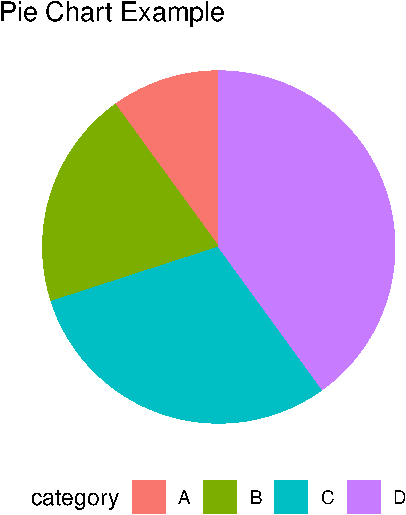
\includegraphics{Line_Graphs_and_Pie_Charts_files/figure-pdf/unnamed-chunk-17-1.pdf}

\section*{Exercises}\label{exercises-4}
\addcontentsline{toc}{section}{Exercises}

\markright{Exercises}

In this assignment, you will create line graphs and pie charts using the
\texttt{ggplot2} library in R. You will use built-in datasets from
RStudio to visualize different types of data. Ensure you follow the
instructions for each problem carefully.

\subsection*{\texorpdfstring{Problem 1: Line Graph of \texttt{pressure}
Dataset}{Problem 1: Line Graph of pressure Dataset}}\label{problem-1-line-graph-of-pressure-dataset}
\addcontentsline{toc}{subsection}{Problem 1: Line Graph of
\texttt{pressure} Dataset}

\textbf{Task:} Create a line graph of the \texttt{pressure} dataset,
which shows the relationship between temperature and pressure.

\textbf{Steps:} 1. Load the \texttt{ggplot2} library. 2. Use the
\texttt{pressure} dataset. 3. Create a line graph with temperature on
the x-axis and pressure on the y-axis. 4. Add appropriate labels to the
axes and a title to the graph.

\textbf{Code Example:}

\begin{Shaded}
\begin{Highlighting}[]
\CommentTok{\# Load ggplot2 library}
\FunctionTok{library}\NormalTok{(ggplot2)}

\CommentTok{\# Create line graph}
\FunctionTok{ggplot}\NormalTok{(pressure, }\FunctionTok{aes}\NormalTok{(}\AttributeTok{x =}\NormalTok{ temperature, }\AttributeTok{y =}\NormalTok{ pressure)) }\SpecialCharTok{+}
  \FunctionTok{geom\_line}\NormalTok{() }\SpecialCharTok{+}
  \FunctionTok{labs}\NormalTok{(}\AttributeTok{title =} \StringTok{"Temperature vs Pressure"}\NormalTok{,}
       \AttributeTok{x =} \StringTok{"Temperature"}\NormalTok{,}
       \AttributeTok{y =} \StringTok{"Pressure"}\NormalTok{)}
\end{Highlighting}
\end{Shaded}

\includegraphics{Line_Graphs_and_Pie_Charts_files/figure-pdf/unnamed-chunk-18-1.pdf}

\subsection*{\texorpdfstring{Problem 2: Line Graph of
\texttt{AirPassengers}
Dataset}{Problem 2: Line Graph of AirPassengers Dataset}}\label{problem-2-line-graph-of-airpassengers-dataset}
\addcontentsline{toc}{subsection}{Problem 2: Line Graph of
\texttt{AirPassengers} Dataset}

\textbf{Task:} Create a line graph of the \texttt{AirPassengers}
dataset, which shows the number of air passengers over time.

\textbf{Steps:} 1. Load the \texttt{ggplot2} library. 2. Use the
\texttt{AirPassengers} dataset. 3. Convert the \texttt{AirPassengers}
time series object to a data frame. 4. Create a line graph with time on
the x-axis and the number of passengers on the y-axis. 5. Add
appropriate labels to the axes and a title to the graph.

\textbf{Code Example:}

\begin{Shaded}
\begin{Highlighting}[]
\CommentTok{\# Load ggplot2 library}
\FunctionTok{library}\NormalTok{(ggplot2)}

\CommentTok{\# Convert AirPassengers to data frame}
\NormalTok{airpassengers\_df }\OtherTok{\textless{}{-}} \FunctionTok{data.frame}\NormalTok{(}
  \AttributeTok{time =} \FunctionTok{time}\NormalTok{(AirPassengers),}
  \AttributeTok{passengers =} \FunctionTok{as.numeric}\NormalTok{(AirPassengers)}
\NormalTok{)}

\CommentTok{\# Create line graph}
\FunctionTok{ggplot}\NormalTok{(airpassengers\_df, }\FunctionTok{aes}\NormalTok{(}\AttributeTok{x =}\NormalTok{ time, }\AttributeTok{y =}\NormalTok{ passengers)) }\SpecialCharTok{+}
  \FunctionTok{geom\_line}\NormalTok{() }\SpecialCharTok{+}
  \FunctionTok{labs}\NormalTok{(}\AttributeTok{title =} \StringTok{"Number of Air Passengers Over Time"}\NormalTok{,}
       \AttributeTok{x =} \StringTok{"Time"}\NormalTok{,}
       \AttributeTok{y =} \StringTok{"Number of Passengers"}\NormalTok{)}
\end{Highlighting}
\end{Shaded}

\begin{verbatim}
Don't know how to automatically pick scale for object of type <ts>. Defaulting
to continuous.
\end{verbatim}

\includegraphics{Line_Graphs_and_Pie_Charts_files/figure-pdf/unnamed-chunk-19-1.pdf}

\subsection*{\texorpdfstring{Problem 3: Line Graph of \texttt{lynx}
Dataset}{Problem 3: Line Graph of lynx Dataset}}\label{problem-3-line-graph-of-lynx-dataset}
\addcontentsline{toc}{subsection}{Problem 3: Line Graph of \texttt{lynx}
Dataset}

\textbf{Task:} Create a line graph of the \texttt{lynx} dataset, which
shows the annual numbers of lynx trappings from 1821--1934 in Canada.

\textbf{Steps:} 1. Load the \texttt{ggplot2} library. 2. Use the
\texttt{lynx} dataset. 3. Convert the \texttt{lynx} time series object
to a data frame. 4. Create a line graph with time on the x-axis and the
number of lynx trapped on the y-axis. 5. Add appropriate labels to the
axes and a title to the graph.

\textbf{Code Example:}

\begin{Shaded}
\begin{Highlighting}[]
\CommentTok{\# Load ggplot2 library}
\FunctionTok{library}\NormalTok{(ggplot2)}

\CommentTok{\# Convert lynx to data frame}
\NormalTok{lynx\_df }\OtherTok{\textless{}{-}} \FunctionTok{data.frame}\NormalTok{(}
  \AttributeTok{year =} \FunctionTok{time}\NormalTok{(lynx),}
  \AttributeTok{trappings =} \FunctionTok{as.numeric}\NormalTok{(lynx)}
\NormalTok{)}

\CommentTok{\# Create line graph}
\FunctionTok{ggplot}\NormalTok{(lynx\_df, }\FunctionTok{aes}\NormalTok{(}\AttributeTok{x =}\NormalTok{ year, }\AttributeTok{y =}\NormalTok{ trappings)) }\SpecialCharTok{+}
  \FunctionTok{geom\_line}\NormalTok{() }\SpecialCharTok{+}
  \FunctionTok{labs}\NormalTok{(}\AttributeTok{title =} \StringTok{"Annual Numbers of Lynx Trappings"}\NormalTok{,}
       \AttributeTok{x =} \StringTok{"Year"}\NormalTok{,}
       \AttributeTok{y =} \StringTok{"Number of Lynx Trapped"}\NormalTok{)}
\end{Highlighting}
\end{Shaded}

\begin{verbatim}
Don't know how to automatically pick scale for object of type <ts>. Defaulting
to continuous.
\end{verbatim}

\includegraphics{Line_Graphs_and_Pie_Charts_files/figure-pdf/unnamed-chunk-20-1.pdf}

\subsection*{\texorpdfstring{Problem 4: Line Graph of \texttt{economics}
Dataset}{Problem 4: Line Graph of economics Dataset}}\label{problem-4-line-graph-of-economics-dataset}
\addcontentsline{toc}{subsection}{Problem 4: Line Graph of
\texttt{economics} Dataset}

\textbf{Task:} Create a line graph of the \texttt{economics} dataset,
which shows the unemployment rate over time.

\textbf{Steps:} 1. Load the \texttt{ggplot2} library. 2. Use the
\texttt{economics} dataset. 3. Create a line graph with date on the
x-axis and unemployment rate (\texttt{unemploy/pop\ *\ 100}) on the
y-axis. 4. Add appropriate labels to the axes and a title to the graph.

\textbf{Code Example:}

\begin{Shaded}
\begin{Highlighting}[]
\CommentTok{\# Load ggplot2 library}
\FunctionTok{library}\NormalTok{(ggplot2)}

\CommentTok{\# Create line graph}
\FunctionTok{ggplot}\NormalTok{(economics, }\FunctionTok{aes}\NormalTok{(}\AttributeTok{x =}\NormalTok{ date, }\AttributeTok{y =}\NormalTok{ unemploy }\SpecialCharTok{/}\NormalTok{ pop }\SpecialCharTok{*} \DecValTok{100}\NormalTok{)) }\SpecialCharTok{+}
  \FunctionTok{geom\_line}\NormalTok{() }\SpecialCharTok{+}
  \FunctionTok{labs}\NormalTok{(}\AttributeTok{title =} \StringTok{"Unemployment Rate Over Time"}\NormalTok{,}
       \AttributeTok{x =} \StringTok{"Date"}\NormalTok{,}
       \AttributeTok{y =} \StringTok{"Unemployment Rate (\%)"}\NormalTok{)}
\end{Highlighting}
\end{Shaded}

\includegraphics{Line_Graphs_and_Pie_Charts_files/figure-pdf/unnamed-chunk-21-1.pdf}

\subsection*{\texorpdfstring{Problem 5: Line Graph of \texttt{co2}
Dataset}{Problem 5: Line Graph of co2 Dataset}}\label{problem-5-line-graph-of-co2-dataset}
\addcontentsline{toc}{subsection}{Problem 5: Line Graph of \texttt{co2}
Dataset}

\textbf{Task:} Create a line graph of the \texttt{co2} dataset, which
shows the concentration of atmospheric carbon dioxide over time.

\textbf{Steps:} 1. Load the \texttt{ggplot2} library. 2. Use the
\texttt{co2} dataset. 3. Convert the \texttt{co2} time series object to
a data frame. 4. Create a line graph with time on the x-axis and CO2
concentration on the y-axis. 5. Add appropriate labels to the axes and a
title to the graph.

\textbf{Code Example:}

\begin{Shaded}
\begin{Highlighting}[]
\CommentTok{\# Load ggplot2 library}
\FunctionTok{library}\NormalTok{(ggplot2)}

\CommentTok{\# Convert co2 to data frame}
\NormalTok{co2\_df }\OtherTok{\textless{}{-}} \FunctionTok{data.frame}\NormalTok{(}
  \AttributeTok{time =} \FunctionTok{time}\NormalTok{(co2),}
  \AttributeTok{concentration =} \FunctionTok{as.numeric}\NormalTok{(co2)}
\NormalTok{)}

\CommentTok{\# Create line graph}
\FunctionTok{ggplot}\NormalTok{(co2\_df, }\FunctionTok{aes}\NormalTok{(}\AttributeTok{x =}\NormalTok{ time, }\AttributeTok{y =}\NormalTok{ concentration)) }\SpecialCharTok{+}
  \FunctionTok{geom\_line}\NormalTok{() }\SpecialCharTok{+}
  \FunctionTok{labs}\NormalTok{(}\AttributeTok{title =} \StringTok{"Atmospheric CO2 Concentration Over Time"}\NormalTok{,}
       \AttributeTok{x =} \StringTok{"Time"}\NormalTok{,}
       \AttributeTok{y =} \StringTok{"CO2 Concentration (ppm)"}\NormalTok{)}
\end{Highlighting}
\end{Shaded}

\begin{verbatim}
Don't know how to automatically pick scale for object of type <ts>. Defaulting
to continuous.
\end{verbatim}

\includegraphics{Line_Graphs_and_Pie_Charts_files/figure-pdf/unnamed-chunk-22-1.pdf}

\subsection*{Problem 6: Pie Chart of Species Distribution in the Iris
Dataset}\label{problem-6-pie-chart-of-species-distribution-in-the-iris-dataset}
\addcontentsline{toc}{subsection}{Problem 6: Pie Chart of Species
Distribution in the Iris Dataset}

\textbf{Objective:} Create a pie chart to visualize the distribution of
different species in the Iris dataset.

\textbf{Steps:} 1. Load the \texttt{ggplot2} library. 2. Use the
built-in \texttt{iris} dataset. 3. Create a data frame that counts the
number of occurrences of each species. 4. Use \texttt{ggplot2} to create
a pie chart displaying the species distribution.

\textbf{Hints:} - Use \texttt{table} to count the occurrences of each
species. - Use \texttt{geom\_bar} and \texttt{coord\_polar} to create
the pie chart.

\textbf{Code Example:}

\begin{Shaded}
\begin{Highlighting}[]
\CommentTok{\# Load ggplot2}
\FunctionTok{library}\NormalTok{(ggplot2)}

\CommentTok{\# Load iris dataset}
\FunctionTok{data}\NormalTok{(iris)}

\CommentTok{\# Count species occurrences}
\NormalTok{species\_count }\OtherTok{\textless{}{-}} \FunctionTok{as.data.frame}\NormalTok{(}\FunctionTok{table}\NormalTok{(iris}\SpecialCharTok{$}\NormalTok{Species))}

\CommentTok{\# Create pie chart}
\FunctionTok{ggplot}\NormalTok{(species\_count, }\FunctionTok{aes}\NormalTok{(}\AttributeTok{x =} \StringTok{""}\NormalTok{, }\AttributeTok{y =}\NormalTok{ Freq, }\AttributeTok{fill =}\NormalTok{ Var1)) }\SpecialCharTok{+}
  \FunctionTok{geom\_bar}\NormalTok{(}\AttributeTok{stat =} \StringTok{"identity"}\NormalTok{, }\AttributeTok{width =} \DecValTok{1}\NormalTok{) }\SpecialCharTok{+}
  \FunctionTok{coord\_polar}\NormalTok{(}\AttributeTok{theta =} \StringTok{"y"}\NormalTok{) }\SpecialCharTok{+} 
  \FunctionTok{geom\_text}\NormalTok{(}\FunctionTok{aes}\NormalTok{(}\AttributeTok{label =}\NormalTok{ Freq),}
        \AttributeTok{position =} \FunctionTok{position\_stack}\NormalTok{(}\AttributeTok{vjust =} \FloatTok{0.5}\NormalTok{),}
        \AttributeTok{color =} \StringTok{"white"}\NormalTok{, }\AttributeTok{size =} \DecValTok{5}\NormalTok{) }\SpecialCharTok{+}
  \FunctionTok{theme\_void}\NormalTok{() }\SpecialCharTok{+}
  \FunctionTok{ggtitle}\NormalTok{(}\StringTok{"Distribution of Species in the Iris Dataset"}\NormalTok{) }\SpecialCharTok{+}
  \FunctionTok{labs}\NormalTok{(}\AttributeTok{fill =} \StringTok{"Species"}\NormalTok{)}
\end{Highlighting}
\end{Shaded}

\includegraphics{Line_Graphs_and_Pie_Charts_files/figure-pdf/unnamed-chunk-23-1.pdf}

\subsection*{Problem 7: Pie Chart of Gear Distribution in the Cars
Dataset}\label{problem-7-pie-chart-of-gear-distribution-in-the-cars-dataset}
\addcontentsline{toc}{subsection}{Problem 7: Pie Chart of Gear
Distribution in the Cars Dataset}

\textbf{Objective:} Create a pie chart to visualize the distribution of
different gears in the \texttt{cars} dataset.

\textbf{Steps:} 1. Load the \texttt{ggplot2} library. 2. Use the
built-in \texttt{cars} dataset. 3. Create a data frame that counts the
number of occurrences of each gear type. 4. Use \texttt{ggplot2} to
create a pie chart displaying the gear distribution.

\textbf{Hints:} - Use \texttt{table} to count the occurrences of each
gear type. - Use \texttt{geom\_bar} and \texttt{coord\_polar} to create
the pie chart.

\textbf{Code Example:}

\begin{Shaded}
\begin{Highlighting}[]
\CommentTok{\# Load ggplot2}
\FunctionTok{library}\NormalTok{(ggplot2)}

\CommentTok{\# Load cars dataset}
\FunctionTok{data}\NormalTok{(mtcars)}

\CommentTok{\# Count gear occurrences}
\NormalTok{gear\_count }\OtherTok{\textless{}{-}} \FunctionTok{as.data.frame}\NormalTok{(}\FunctionTok{table}\NormalTok{(mtcars}\SpecialCharTok{$}\NormalTok{gear))}

\CommentTok{\# Create pie chart}

\FunctionTok{ggplot}\NormalTok{(gear\_count, }\FunctionTok{aes}\NormalTok{(}\AttributeTok{x =} \StringTok{""}\NormalTok{, }\AttributeTok{y =}\NormalTok{ Freq, }\AttributeTok{fill =}\NormalTok{ Var1)) }\SpecialCharTok{+}
  \FunctionTok{geom\_bar}\NormalTok{(}\AttributeTok{stat =} \StringTok{"identity"}\NormalTok{, }\AttributeTok{width =} \DecValTok{1}\NormalTok{) }\SpecialCharTok{+}
  \FunctionTok{coord\_polar}\NormalTok{(}\AttributeTok{theta =} \StringTok{"y"}\NormalTok{) }\SpecialCharTok{+} 
  \FunctionTok{geom\_text}\NormalTok{(}\FunctionTok{aes}\NormalTok{(}\AttributeTok{label =}\NormalTok{ Freq),}
        \AttributeTok{position =} \FunctionTok{position\_stack}\NormalTok{(}\AttributeTok{vjust =} \FloatTok{0.5}\NormalTok{),}
        \AttributeTok{color =} \StringTok{"white"}\NormalTok{, }\AttributeTok{size =} \DecValTok{5}\NormalTok{) }\SpecialCharTok{+}
  \FunctionTok{theme\_void}\NormalTok{() }\SpecialCharTok{+}
  \FunctionTok{ggtitle}\NormalTok{(}\StringTok{"Distribution of Gears in the Cars Dataset"}\NormalTok{) }\SpecialCharTok{+}
  \FunctionTok{labs}\NormalTok{(}\AttributeTok{fill =} \StringTok{"Gears"}\NormalTok{)}
\end{Highlighting}
\end{Shaded}

\includegraphics{Line_Graphs_and_Pie_Charts_files/figure-pdf/unnamed-chunk-24-1.pdf}

\subsection*{Problem 8: Pie Chart of Titanic Class Distribution in the
Titanic
Dataset}\label{problem-8-pie-chart-of-titanic-class-distribution-in-the-titanic-dataset}
\addcontentsline{toc}{subsection}{Problem 8: Pie Chart of Titanic Class
Distribution in the Titanic Dataset}

\textbf{Objective:} Create a pie chart to visualize the distribution of
different classes in the \texttt{Titanic} dataset.

\textbf{Steps:} 1. Load the \texttt{ggplot2} library. 2. Use the
built-in \texttt{Titanic} dataset. 3. Create a data frame that counts
the number of occurrences of each class. 4. Use \texttt{ggplot2} to
create a pie chart displaying the class distribution.

\textbf{Hints:} - Use \texttt{table} to count the occurrences of each
class. - Use \texttt{geom\_bar} and \texttt{coord\_polar} to create the
pie chart.

\textbf{Code Example:}

\begin{Shaded}
\begin{Highlighting}[]
\CommentTok{\# Load ggplot2}
\FunctionTok{library}\NormalTok{(ggplot2)}

\CommentTok{\# Load Titanic dataset}
\FunctionTok{data}\NormalTok{(Titanic)}

\CommentTok{\# Convert Titanic dataset to data frame}
\NormalTok{titanic\_df }\OtherTok{\textless{}{-}} \FunctionTok{as.data.frame}\NormalTok{(Titanic)}

\CommentTok{\# Count class occurrences}
\NormalTok{class\_count }\OtherTok{\textless{}{-}} \FunctionTok{as.data.frame}\NormalTok{(}\FunctionTok{table}\NormalTok{(titanic\_df}\SpecialCharTok{$}\NormalTok{Class))}

\CommentTok{\# Create pie chart}
\FunctionTok{ggplot}\NormalTok{(class\_count, }\FunctionTok{aes}\NormalTok{(}\AttributeTok{x =} \StringTok{""}\NormalTok{, }\AttributeTok{y =}\NormalTok{ Freq, }\AttributeTok{fill =}\NormalTok{ Var1)) }\SpecialCharTok{+}
  \FunctionTok{geom\_bar}\NormalTok{(}\AttributeTok{stat =} \StringTok{"identity"}\NormalTok{, }\AttributeTok{width =} \DecValTok{1}\NormalTok{) }\SpecialCharTok{+}
  \FunctionTok{coord\_polar}\NormalTok{(}\AttributeTok{theta =} \StringTok{"y"}\NormalTok{) }\SpecialCharTok{+}
  \FunctionTok{theme\_void}\NormalTok{() }\SpecialCharTok{+}
  \FunctionTok{ggtitle}\NormalTok{(}\StringTok{"Distribution of Classes in the Titanic Dataset"}\NormalTok{) }\SpecialCharTok{+}
  \FunctionTok{labs}\NormalTok{(}\AttributeTok{fill =} \StringTok{"Class"}\NormalTok{)}
\end{Highlighting}
\end{Shaded}

\includegraphics{Line_Graphs_and_Pie_Charts_files/figure-pdf/unnamed-chunk-25-1.pdf}

\subsection*{\texorpdfstring{Problem 9: Pie Chart of Supplement
Distribution in the \texttt{ToothGrowth}
Dataset}{Problem 9: Pie Chart of Supplement Distribution in the ToothGrowth Dataset}}\label{problem-9-pie-chart-of-supplement-distribution-in-the-toothgrowth-dataset}
\addcontentsline{toc}{subsection}{Problem 9: Pie Chart of Supplement
Distribution in the \texttt{ToothGrowth} Dataset}

\textbf{Task:} Create a pie chart to show the distribution of the
different supplements (VC and OJ) in the \texttt{ToothGrowth} dataset.

\textbf{Steps:} 1. Load the \texttt{ggplot2} library and the
\texttt{ToothGrowth} dataset. 2. Create a data frame that summarizes the
count of each supplement type. 3. Use \texttt{ggplot2} to create a pie
chart that shows the proportion of each supplement.

\textbf{Hint:} Use the \texttt{fill} aesthetic to map the \texttt{supp}
column to the pie chart slices.

\textbf{Code Example:}

\begin{Shaded}
\begin{Highlighting}[]
\CommentTok{\# Load ggplot2 and ToothGrowth dataset}
\FunctionTok{library}\NormalTok{(ggplot2)}
\FunctionTok{data}\NormalTok{(ToothGrowth)}

\CommentTok{\# Summarize count of each supplement type}
\NormalTok{supp\_count }\OtherTok{\textless{}{-}} \FunctionTok{as.data.frame}\NormalTok{(}\FunctionTok{table}\NormalTok{(ToothGrowth}\SpecialCharTok{$}\NormalTok{supp))}

\CommentTok{\# Create pie chart}
\FunctionTok{ggplot}\NormalTok{(supp\_count, }\FunctionTok{aes}\NormalTok{(}\AttributeTok{x =} \StringTok{""}\NormalTok{, }\AttributeTok{y =}\NormalTok{ Freq, }\AttributeTok{fill =}\NormalTok{ Var1)) }\SpecialCharTok{+}
  \FunctionTok{geom\_bar}\NormalTok{(}\AttributeTok{stat =} \StringTok{"identity"}\NormalTok{, }\AttributeTok{width =} \DecValTok{1}\NormalTok{) }\SpecialCharTok{+}
  \FunctionTok{coord\_polar}\NormalTok{(}\AttributeTok{theta =} \StringTok{"y"}\NormalTok{) }\SpecialCharTok{+}
  \FunctionTok{labs}\NormalTok{(}\AttributeTok{title =} \StringTok{"Supplement Distribution in ToothGrowth Dataset"}\NormalTok{, }\AttributeTok{fill =} \StringTok{"Supplement"}\NormalTok{) }\SpecialCharTok{+}
  \FunctionTok{theme\_void}\NormalTok{()}
\end{Highlighting}
\end{Shaded}

\includegraphics{Line_Graphs_and_Pie_Charts_files/figure-pdf/unnamed-chunk-26-1.pdf}

\subsection*{\texorpdfstring{Problem 10: Pie Chart of Education Levels
in the \texttt{infert}
Dataset}{Problem 10: Pie Chart of Education Levels in the infert Dataset}}\label{problem-10-pie-chart-of-education-levels-in-the-infert-dataset}
\addcontentsline{toc}{subsection}{Problem 10: Pie Chart of Education
Levels in the \texttt{infert} Dataset}

\textbf{Task:} Create a pie chart to show the distribution of different
education levels in the \texttt{infert} dataset.

\textbf{Steps:} 1. Load the \texttt{ggplot2} library and the
\texttt{infert} dataset. 2. Create a data frame that summarizes the
count of each education level. 3. Use \texttt{ggplot2} to create a pie
chart that shows the proportion of each education level.

\textbf{Hint:} Use the \texttt{fill} aesthetic to map the
\texttt{education} column to the pie chart slices.

\textbf{Code Example:}

\begin{Shaded}
\begin{Highlighting}[]
\CommentTok{\# Load ggplot2 and infert dataset}
\FunctionTok{library}\NormalTok{(ggplot2)}
\FunctionTok{data}\NormalTok{(infert)}

\CommentTok{\# Summarize count of each education level}
\NormalTok{education\_count }\OtherTok{\textless{}{-}} \FunctionTok{as.data.frame}\NormalTok{(}\FunctionTok{table}\NormalTok{(infert}\SpecialCharTok{$}\NormalTok{education))}

\CommentTok{\# Create pie chart}
\FunctionTok{ggplot}\NormalTok{(education\_count, }\FunctionTok{aes}\NormalTok{(}\AttributeTok{x =} \StringTok{""}\NormalTok{, }\AttributeTok{y =}\NormalTok{ Freq, }\AttributeTok{fill =}\NormalTok{ Var1)) }\SpecialCharTok{+}
  \FunctionTok{geom\_bar}\NormalTok{(}\AttributeTok{stat =} \StringTok{"identity"}\NormalTok{, }\AttributeTok{width =} \DecValTok{1}\NormalTok{) }\SpecialCharTok{+}
  \FunctionTok{coord\_polar}\NormalTok{(}\AttributeTok{theta =} \StringTok{"y"}\NormalTok{) }\SpecialCharTok{+} 
  \FunctionTok{geom\_text}\NormalTok{(}\FunctionTok{aes}\NormalTok{(}\AttributeTok{label =}\NormalTok{ Freq),}
        \AttributeTok{position =} \FunctionTok{position\_stack}\NormalTok{(}\AttributeTok{vjust =} \FloatTok{0.5}\NormalTok{),}
        \AttributeTok{color =} \StringTok{"white"}\NormalTok{, }\AttributeTok{size =} \DecValTok{5}\NormalTok{) }\SpecialCharTok{+}
  \FunctionTok{labs}\NormalTok{(}\AttributeTok{title =} \StringTok{"Education Levels in Infert Dataset"}\NormalTok{, }\AttributeTok{fill =} \StringTok{"Education Level"}\NormalTok{) }\SpecialCharTok{+}
  \FunctionTok{theme\_void}\NormalTok{()}
\end{Highlighting}
\end{Shaded}

\includegraphics{Line_Graphs_and_Pie_Charts_files/figure-pdf/unnamed-chunk-27-1.pdf}

\section*{Conclusion}\label{conclusion-1}
\addcontentsline{toc}{section}{Conclusion}

\markright{Conclusion}

In this tutorial, we learned how to create line graphs and pie charts in
R using the \texttt{ggplot2} package. Line graphs are useful for showing
trends over time and comparing multiple data series, while pie charts
are useful for showing the relative proportions of different categories.
By using \texttt{ggplot2}, we can create high-quality visualizations
that help us understand and communicate data more effectively. I hope
you found this tutorial helpful and that you can now create your own
line graphs and pie charts in R. Thank you for reading!

\bookmarksetup{startatroot}

\chapter*{What is ``Tidy Data''?}\label{what-is-tidy-data}
\addcontentsline{toc}{chapter}{What is ``Tidy Data''?}

\markboth{What is ``Tidy Data''?}{What is ``Tidy Data''?}

\begin{tcolorbox}[enhanced jigsaw, toprule=.15mm, colbacktitle=quarto-callout-note-color!10!white, titlerule=0mm, arc=.35mm, breakable, opacityback=0, coltitle=black, opacitybacktitle=0.6, title=\textcolor{quarto-callout-note-color}{\faInfo}\hspace{0.5em}{Note}, left=2mm, bottomtitle=1mm, colback=white, rightrule=.15mm, colframe=quarto-callout-note-color-frame, bottomrule=.15mm, toptitle=1mm, leftrule=.75mm]

FYI : Here is the official page for Tidy data. This page is based off of
the original paper describing tidy data that Hadley Wickham wrote for
the Journal of Statistical Software :
\href{https://vita.had.co.nz/papers/tidy-data.pdf}{Tidy Data}

\end{tcolorbox}

Tidy data is a standard way of organizing data that makes it easy to
work with. It is a concept that was popularized by the
\textbf{tidyverse} packages in R. tidyverse is, in a sense, a
``library'' that contains several packages that are designed to work
together, and are designed to work with tidy data. The tidyverse
packages include the \textbf{dplyr} and \textbf{tidyr} packages among
others. These packages are designed to work with tidy data. As you start
to learn more about \textbf{R}, you will discover several of the
packages included in the \texttt{tidyverse}. These packages are designed
to work with tidy data. The \texttt{tidyverse} packages include several
packages that provide tools for reading in data (the \textbf{readr}
package), cleaning data (the \textbf{dplyr} package), transforming data
(the \textbf{tidyr} package), and visual data (the \textbf{ggplot2}
package). These tools are designed to work with tidy data, so it is
important to understand what tidy data is and how to organize data in a
tidy format.

Hadley Wickham, the author of the \texttt{tidyverse} packages, defines
tidy data as follows:

\begin{enumerate}
\def\labelenumi{\arabic{enumi}.}
\tightlist
\item
  Each variable forms a column.
\item
  Each observation forms a row.
\item
  Each type of observational unit forms a table.
\end{enumerate}

The purpose for creating data sets that are tidy is to make it easier to
analyze and visualize data. Tidy data is easy to work with because it
follows a \textbf{consistent structure} that makes it easy to manipulate
and visualize data. If we know that the data set is set up as a tidy
data set, we can use the \texttt{tidyverse} packages to work with the
data. These packages provide tools that are set up to work with tidy
data.

This consistency makes it easier to read in data, to clean data, to
transform data, and to visualize data. When data is tidy, it is easier
to work with because we can use the same tools to work with the data.
This means we don't have to learn new tools for each new data set that
we work with.

When data is not tidy, it can be difficult to work with. For example, if
data is spread across multiple columns, it can be difficult to analyze
and visualize the data. You may have to completely rewrite your code or
create a completely new script to work with the data. By organizing data
in a tidy format, it is easier to work with and analyze data because we
have these packages that are created to work with a data set that has
been formatted as ``tidy''.

\section*{Example}\label{example}
\addcontentsline{toc}{section}{Example}

\markright{Example}

Consider the following data:

\begin{Shaded}
\begin{Highlighting}[]
\CommentTok{\# If needed, install the tidyverse package}

\CommentTok{\# install.packages("tidyverse")}

\CommentTok{\# If it is already installed, make sure it is loaded up to use :}

\CommentTok{\# Load the tidyverse package}

\FunctionTok{library}\NormalTok{(tidyverse)}
\end{Highlighting}
\end{Shaded}

Let's create a data frame that is not tidy. We will create a data frame
with three rows and four columns. The first column contains the names of
three people, and the other columns contain data for the years 2010,
2011, and 2012. Each row represents a person, and each column represents
their age during that year.

\begin{Shaded}
\begin{Highlighting}[]
\NormalTok{df }\OtherTok{\textless{}{-}} \FunctionTok{tibble}\NormalTok{(}
  \AttributeTok{name =} \FunctionTok{c}\NormalTok{(}\StringTok{"John Smith"}\NormalTok{, }\StringTok{"Jane Doe"}\NormalTok{, }\StringTok{"Mary Johnson"}\NormalTok{),}
  \StringTok{\textasciigrave{}}\AttributeTok{2010}\StringTok{\textasciigrave{}} \OtherTok{=} \FunctionTok{c}\NormalTok{(}\DecValTok{25}\NormalTok{, }\DecValTok{30}\NormalTok{, }\DecValTok{35}\NormalTok{),}
  \StringTok{\textasciigrave{}}\AttributeTok{2011}\StringTok{\textasciigrave{}} \OtherTok{=} \FunctionTok{c}\NormalTok{(}\DecValTok{26}\NormalTok{, }\DecValTok{31}\NormalTok{, }\DecValTok{36}\NormalTok{),}
  \StringTok{\textasciigrave{}}\AttributeTok{2012}\StringTok{\textasciigrave{}} \OtherTok{=} \FunctionTok{c}\NormalTok{(}\DecValTok{27}\NormalTok{, }\DecValTok{32}\NormalTok{, }\DecValTok{37}\NormalTok{)}
\NormalTok{)}

\NormalTok{df}
\end{Highlighting}
\end{Shaded}

\begin{verbatim}
# A tibble: 3 x 4
  name         `2010` `2011` `2012`
  <chr>         <dbl>  <dbl>  <dbl>
1 John Smith       25     26     27
2 Jane Doe         30     31     32
3 Mary Johnson     35     36     37
\end{verbatim}

In this case, the data is not tidy because the years are spread across
columns. In order for this to be considered ``tidy'' data, we would need
to think about the data in a different way.

The variables we are using are \textbf{name}, \textbf{year}, and
\textbf{age}. In order for the data to be tidy, we want each observation
(row) to contain a name, a year, and the age. This tells us we would
need to have a column for each of these variables. In this case, we
would need to have a column for the name of the person, a column for the
year that the data was collected, and a column for the age of the person
the year the data was collected.

Here is what the tidy data would look like if we ordered the data in a
tidy format by name, year, and age:

\begin{Shaded}
\begin{Highlighting}[]
\NormalTok{df\_tidy }\OtherTok{\textless{}{-}} \FunctionTok{tibble}\NormalTok{(}
  \AttributeTok{name =} \FunctionTok{c}\NormalTok{(}\StringTok{"John Smith"}\NormalTok{, }\StringTok{"John Smith"}\NormalTok{, }\StringTok{"John Smith"}\NormalTok{, }\StringTok{"Jane Doe"}\NormalTok{, }\StringTok{"Jane Doe"}\NormalTok{, }
           \StringTok{"Jane Doe"}\NormalTok{, }\StringTok{"Mary Johnson"}\NormalTok{, }\StringTok{"Mary Johnson"}\NormalTok{, }\StringTok{"Mary Johnson"}\NormalTok{),}
  \AttributeTok{year =} \FunctionTok{c}\NormalTok{(}\DecValTok{2010}\NormalTok{, }\DecValTok{2011}\NormalTok{, }\DecValTok{2012}\NormalTok{, }\DecValTok{2010}\NormalTok{, }\DecValTok{2011}\NormalTok{, }\DecValTok{2012}\NormalTok{, }\DecValTok{2010}\NormalTok{, }\DecValTok{2011}\NormalTok{, }\DecValTok{2012}\NormalTok{),}
  \AttributeTok{age =} \FunctionTok{c}\NormalTok{(}\DecValTok{25}\NormalTok{, }\DecValTok{26}\NormalTok{, }\DecValTok{27}\NormalTok{, }\DecValTok{30}\NormalTok{, }\DecValTok{31}\NormalTok{, }\DecValTok{32}\NormalTok{, }\DecValTok{35}\NormalTok{, }\DecValTok{36}\NormalTok{, }\DecValTok{37}\NormalTok{)}
\NormalTok{)}

\NormalTok{df\_tidy}
\end{Highlighting}
\end{Shaded}

\begin{verbatim}
# A tibble: 9 x 3
  name          year   age
  <chr>        <dbl> <dbl>
1 John Smith    2010    25
2 John Smith    2011    26
3 John Smith    2012    27
4 Jane Doe      2010    30
5 Jane Doe      2011    31
6 Jane Doe      2012    32
7 Mary Johnson  2010    35
8 Mary Johnson  2011    36
9 Mary Johnson  2012    37
\end{verbatim}

We have now \textbf{cleaned} the data so that we can work with it in a
tidy format.

As an example of how you could use the tools from the tidyverse package,
you could use the \textbf{pivot\_longer( )} function from the
\textbf{tidyr} package to convert the data from the original data frame
to a tidy data frame. This is just an example to show you a more elegant
way to convert the data to a tidy format. You will perform more advanced
cleaning options as you learn more about the tidyverse packages.

\begin{Shaded}
\begin{Highlighting}[]
\NormalTok{df\_tidy }\OtherTok{\textless{}{-}}\NormalTok{ df }\SpecialCharTok{\%\textgreater{}\%} 
  \FunctionTok{pivot\_longer}\NormalTok{(}\AttributeTok{cols =} \SpecialCharTok{{-}}\NormalTok{name, }\AttributeTok{names\_to =} \StringTok{"year"}\NormalTok{, }\AttributeTok{values\_to =} \StringTok{"value"}\NormalTok{)}

\NormalTok{df\_tidy}
\end{Highlighting}
\end{Shaded}

\begin{verbatim}
# A tibble: 9 x 3
  name         year  value
  <chr>        <chr> <dbl>
1 John Smith   2010     25
2 John Smith   2011     26
3 John Smith   2012     27
4 Jane Doe     2010     30
5 Jane Doe     2011     31
6 Jane Doe     2012     32
7 Mary Johnson 2010     35
8 Mary Johnson 2011     36
9 Mary Johnson 2012     37
\end{verbatim}

Now the data is tidy because each variable forms a column, each
observation forms a row, and each type of observational unit forms a
table.

\section*{Summary}\label{summary}
\addcontentsline{toc}{section}{Summary}

\markright{Summary}

Tidy data is a standard way of organizing data that makes it easy to
work with. The \texttt{tidyverse} packages provide tools for working
with tidy data, making it easier to analyze and visualize data.

\begin{center}\rule{0.5\linewidth}{0.5pt}\end{center}

\section*{Exercises}\label{exercises-5}
\addcontentsline{toc}{section}{Exercises}

\markright{Exercises}

In this assignment, you will identify whether a given dataset is in tidy
format. Each problem will present a dataset from a different background
along with a brief description. Your task is to determine if the dataset
is tidy. If it is not tidy, describe why and provide a tidy version of
the dataset.

\subsection*{Problem 1: Weather Data}\label{problem-1-weather-data}
\addcontentsline{toc}{subsection}{Problem 1: Weather Data}

The following dataset contains weather data for three cities.

\begin{tabular}{l|r|r|r}
\hline
City & Jan\_Temp & Feb\_Temp & Mar\_Temp\\
\hline
New York & 30 & 32 & 45\\
\hline
Los Angeles & 58 & 60 & 65\\
\hline
Chicago & 25 & 28 & 40\\
\hline
\end{tabular}

\subsection*{Problem 2: Student Grades}\label{problem-2-student-grades}
\addcontentsline{toc}{subsection}{Problem 2: Student Grades}

The following dataset contains grades for students in three subjects.

\begin{table}
\centering
\begin{tabular}{l|r|r|r}
\hline
Student & Math & Science & History\\
\hline
Alice & 90 & 88 & 84\\
\hline
Bob & 85 & 92 & 78\\
\hline
Charlie & 95 & 89 & 91\\
\hline
\end{tabular}
\end{table}

\subsection*{Problem 3: Sales Data}\label{problem-3-sales-data}
\addcontentsline{toc}{subsection}{Problem 3: Sales Data}

The following dataset contains monthly sales data for different
products.

\begin{table}
\centering
\begin{tabular}{l|r|r|r}
\hline
Product & Jan\_Sales & Feb\_Sales & Mar\_Sales\\
\hline
A & 100 & 110 & 120\\
\hline
B & 150 & 160 & 170\\
\hline
C & 200 & 210 & 220\\
\hline
\end{tabular}
\end{table}

\subsection*{Problem 4: Patient Health
Data}\label{problem-4-patient-health-data}
\addcontentsline{toc}{subsection}{Problem 4: Patient Health Data}

The following dataset contains health data for patients.

\begin{table}
\centering
\begin{tabular}{l|r|r|r}
\hline
Patient & Height & Weight & Age\\
\hline
John & 170 & 70 & 30\\
\hline
Jane & 160 & 55 & 25\\
\hline
Doe & 180 & 80 & 40\\
\hline
\end{tabular}
\end{table}

\subsection*{Problem 5: Financial Data}\label{problem-5-financial-data}
\addcontentsline{toc}{subsection}{Problem 5: Financial Data}

The following dataset contains quarterly financial data for companies.

\begin{table}
\centering
\begin{tabular}{l|r|r|r}
\hline
Company & Q1\_Revenue & Q2\_Revenue & Q3\_Revenue\\
\hline
X & 1000 & 1100 & 1200\\
\hline
Y & 2000 & 2100 & 2200\\
\hline
Z & 3000 & 3100 & 3200\\
\hline
\end{tabular}
\end{table}

\subsection*{Problem 6: Sports
Statistics}\label{problem-6-sports-statistics}
\addcontentsline{toc}{subsection}{Problem 6: Sports Statistics}

The following dataset contains statistics for players in a sports team.

\begin{table}
\centering
\begin{tabular}{l|r|r|r}
\hline
Player & Goals & Assists & Saves\\
\hline
Player1 & 5 & 3 & 2\\
\hline
Player2 & 8 & 5 & 1\\
\hline
Player3 & 7 & 4 & 3\\
\hline
\end{tabular}
\end{table}

\subsection*{Problem 7: Movie Ratings}\label{problem-7-movie-ratings}
\addcontentsline{toc}{subsection}{Problem 7: Movie Ratings}

The following dataset contains ratings for movies by different critics.

\begin{table}
\centering
\begin{tabular}{l|r|r|r}
\hline
Movie & Critic1 & Critic2 & Critic3\\
\hline
Movie A & 4.5 & 4.0 & 4.7\\
\hline
Movie B & 3.8 & 3.9 & 4.0\\
\hline
Movie C & 4.7 & 4.8 & 4.9\\
\hline
\end{tabular}
\end{table}

\subsection*{Problem 8: Employee Salary
Data}\label{problem-8-employee-salary-data}
\addcontentsline{toc}{subsection}{Problem 8: Employee Salary Data}

The following dataset contains salary data for employees in different
departments.

\begin{table}
\centering
\begin{tabular}{l|r|r|r}
\hline
Employee & Dept1\_Salary & Dept2\_Salary & Dept3\_Salary\\
\hline
E1 & 50000 & 52000 & 54000\\
\hline
E2 & 55000 & 57000 & 59000\\
\hline
E3 & 60000 & 62000 & 64000\\
\hline
\end{tabular}
\end{table}

\subsection*{Problem 9: Product
Reviews}\label{problem-9-product-reviews}
\addcontentsline{toc}{subsection}{Problem 9: Product Reviews}

The following dataset contains reviews for products.

\begin{table}
\centering
\begin{tabular}{l|l|l|l}
\hline
Product & Review1 & Review2 & Review3\\
\hline
Product1 & Good & Very Good & Excellent\\
\hline
Product2 & Average & Good & Good\\
\hline
Product3 & Excellent & Very Good & Good\\
\hline
\end{tabular}
\end{table}

\subsection*{Problem 10: Course Enrollment
Data}\label{problem-10-course-enrollment-data}
\addcontentsline{toc}{subsection}{Problem 10: Course Enrollment Data}

The following dataset contains enrollment data for courses.

\begin{table}
\centering
\begin{tabular}{l|r|r|r}
\hline
Course & Semester1 & Semester2 & Semester3\\
\hline
Course1 & 30 & 35 & 32\\
\hline
Course2 & 25 & 28 & 26\\
\hline
Course3 & 20 & 22 & 24\\
\hline
\end{tabular}
\end{table}

\subsection*{Problem 11: Sales Data}\label{problem-11-sales-data}
\addcontentsline{toc}{subsection}{Problem 11: Sales Data}

The following table shows the monthly sales data for three products.

\begin{table}
\centering
\begin{tabular}{l|r|r|r}
\hline
Product & January & February & March\\
\hline
Product A & 100 & 120 & 130\\
\hline
Product B & 150 & 160 & 170\\
\hline
Product C & 200 & 220 & 230\\
\hline
\end{tabular}
\end{table}

\subsection*{Problem 12: Survey Data}\label{problem-12-survey-data}
\addcontentsline{toc}{subsection}{Problem 12: Survey Data}

The following table represents the results of a survey where respondents
rated their satisfaction with three services.

\begin{table}
\centering
\begin{tabular}{l|r|r|r}
\hline
Respondent & Service1\_Satisfaction & Service2\_Satisfaction & Service3\_Satisfaction\\
\hline
R1 & 5 & 4 & 3\\
\hline
R2 & 4 & 3 & 2\\
\hline
R3 & 3 & 2 & 1\\
\hline
\end{tabular}
\end{table}

\subsection*{Problem 13: Weather Data}\label{problem-13-weather-data}
\addcontentsline{toc}{subsection}{Problem 13: Weather Data}

The table below shows the temperature readings at different times of the
day for a week.

\begin{table}
\centering
\begin{tabular}{l|r|r|r}
\hline
Day & Morning & Noon & Evening\\
\hline
Monday & 20 & 25 & 22\\
\hline
Tuesday & 21 & 26 & 23\\
\hline
Wednesday & 19 & 24 & 21\\
\hline
Thursday & 22 & 27 & 24\\
\hline
Friday & 20 & 25 & 22\\
\hline
\end{tabular}
\end{table}

\subsection*{Problem 14: Exam Scores}\label{problem-14-exam-scores}
\addcontentsline{toc}{subsection}{Problem 14: Exam Scores}

The following table lists the scores of students in three subjects.

\begin{table}
\centering
\begin{tabular}{l|r|r|r}
\hline
Student & Math & Science & History\\
\hline
Student1 & 85 & 88 & 80\\
\hline
Student2 & 90 & 92 & 85\\
\hline
Student3 & 95 & 96 & 90\\
\hline
\end{tabular}
\end{table}

\subsection*{Problem 15: Hospital Data}\label{problem-15-hospital-data}
\addcontentsline{toc}{subsection}{Problem 15: Hospital Data}

The table below shows the number of patients admitted to different wards
of a hospital over three months.

\begin{table}
\centering
\begin{tabular}{l|r|r|r}
\hline
Ward & January & February & March\\
\hline
Ward A & 30 & 35 & 40\\
\hline
Ward B & 25 & 30 & 35\\
\hline
Ward C & 20 & 25 & 30\\
\hline
\end{tabular}
\end{table}

\subsection*{Problem 16: Marketing
Data}\label{problem-16-marketing-data}
\addcontentsline{toc}{subsection}{Problem 16: Marketing Data}

The following table represents the results of a marketing campaign
showing the number of leads generated from different channels.

\begin{table}
\centering
\begin{tabular}{l|r|r|r}
\hline
Channel & Week1 & Week2 & Week3\\
\hline
Email & 50 & 55 & 60\\
\hline
Social Media & 60 & 65 & 70\\
\hline
SEO & 70 & 75 & 80\\
\hline
\end{tabular}
\end{table}

\subsection*{Problem 17: Fitness Data}\label{problem-17-fitness-data}
\addcontentsline{toc}{subsection}{Problem 17: Fitness Data}

The table below shows the workouts completed by three athletes over a
week.

\begin{table}
\centering
\begin{tabular}{l|r|r|r}
\hline
Athlete & Monday & Wednesday & Friday\\
\hline
Athlete1 & 30 & 35 & 40\\
\hline
Athlete2 & 40 & 45 & 50\\
\hline
Athlete3 & 50 & 55 & 60\\
\hline
\end{tabular}
\end{table}

\subsection*{Problem 18: Financial
Data}\label{problem-18-financial-data}
\addcontentsline{toc}{subsection}{Problem 18: Financial Data}

The following table shows the quarterly profits for three companies.

\begin{table}
\centering
\begin{tabular}{l|r|r|r|r}
\hline
Company & Q1 & Q2 & Q3 & Q4\\
\hline
Company A & 10000 & 12000 & 13000 & 14000\\
\hline
Company B & 15000 & 16000 & 17000 & 18000\\
\hline
Company C & 20000 & 22000 & 23000 & 24000\\
\hline
\end{tabular}
\end{table}

\subsection*{Problem 19: Attendance
Data}\label{problem-19-attendance-data}
\addcontentsline{toc}{subsection}{Problem 19: Attendance Data}

The table below shows the attendance numbers for different events over
three days.

\begin{table}
\centering
\begin{tabular}{l|r|r|r}
\hline
Event & Day1 & Day2 & Day3\\
\hline
Event A & 100 & 110 & 120\\
\hline
Event B & 150 & 160 & 170\\
\hline
Event C & 200 & 210 & 220\\
\hline
\end{tabular}
\end{table}

\subsection*{Problem 20: Production
Data}\label{problem-20-production-data}
\addcontentsline{toc}{subsection}{Problem 20: Production Data}

The following table represents the production output of different
products over three shifts.

\begin{table}
\centering
\begin{tabular}{l|r|r|r}
\hline
Product & Shift1 & Shift2 & Shift3\\
\hline
Product X & 300 & 350 & 400\\
\hline
Product Y & 400 & 450 & 500\\
\hline
Product Z & 500 & 550 & 600\\
\hline
\end{tabular}
\end{table}

\bookmarksetup{startatroot}

\chapter*{Beginning Data
Visualization}\label{beginning-data-visualization}
\addcontentsline{toc}{chapter}{Beginning Data Visualization}

\markboth{Beginning Data Visualization}{Beginning Data Visualization}

This section will walk you through the beginning steps for how to
visualize your data using \textbf{ggplot2}. R has several systems for
making graphs, but ggplot2 is one of the most elegant and most
versatile. ggplot2 implements the grammar of graphics, a coherent system
for describing and building graphs. With ggplot2, you can do more faster
by learning one system and applying it in many places.

This ssection focuses on ggplot2, one of the core packages of the
\textbf{tidyverse} library. To access the datasets, help pages, and
functions that we will use in this section, load the tidyverse library
by running this code in the console, in your script, or by checking the
tidyverse box in the \textbf{Packages} tab in RStudio. Note that if it
does not appear in the Packages tab then it is not installed and you
will have to install tidyverse before you can load it up.

\includegraphics[width=0.75\textwidth,height=\textheight]{./images/Daily-2-Pic-1.jpg}

That one line of code loads the core tidyverse; packages which you will
use in almost every data analysis. It also tells you which functions
from the tidyverse conflict with functions in base R (or from other
packages you might have loaded).

If you run this code and get the error message ``\emph{there is no
package called `tidyverse'}'', you'll need to first install it, then run
\textbf{library()} once again.

You only need to install a package once, but you need to reload it every
time you start a new session. If we need to be explicit about where a
function (or dataset) comes from, we'll use the special form
\textbf{package::function()}. For example, \textbf{ggplot2::ggplot()}
tells you explicitly that we're using the \textbf{ggplot()} function
from the \textbf{ggplot2} package.

Let's use our first graph to answer a question: Do cars with big engines
use more fuel than cars with small engines? You probably already have an
answer, but try to make your answer precise. What does the relationship
between engine size and fuel efficiency look like?

You can test your answer with the mpg data frame found in ggplot2 (aka
\textbf{ggplot2::mpg}). A data frame is a rectangular collection of
variables (in the columns) and observations (in the rows). mpg contains
observations collected by the US Environmental Protection Agency on 38
models of car.

\includegraphics[width=0.75\textwidth,height=\textheight]{./images/Daily-2-Pic-2.jpg}

A few examples of the variables in \textbf{mpg} are:

\begin{enumerate}
\def\labelenumi{\arabic{enumi}.}
\item
  \textbf{displ}, a car's engine size, in litres.
\item
  \textbf{hwy}, a car's fuel efficiency on the highway, in miles per
  gallon (mpg). A car with a low fuel efficiency consumes more fuel than
  a car with a high fuel efficiency when they travel the same distance.
\end{enumerate}

To learn more about \textbf{mpg}, open its help page by running
\textbf{?mpg}.

To plot mpg, run this code to put \textbf{displ} on the x-axis and
\textbf{hwy} on the y-axis:

\begin{Shaded}
\begin{Highlighting}[]
\FunctionTok{library}\NormalTok{(tidyverse)}
\end{Highlighting}
\end{Shaded}

\begin{verbatim}
-- Attaching core tidyverse packages ------------------------ tidyverse 2.0.0 --
v dplyr     1.1.4     v readr     2.1.5
v forcats   1.0.0     v stringr   1.5.1
v ggplot2   3.5.1     v tibble    3.2.1
v lubridate 1.9.4     v tidyr     1.3.1
v purrr     1.0.2     
-- Conflicts ------------------------------------------ tidyverse_conflicts() --
x dplyr::filter() masks stats::filter()
x dplyr::lag()    masks stats::lag()
i Use the conflicted package (<http://conflicted.r-lib.org/>) to force all conflicts to become errors
\end{verbatim}

\begin{Shaded}
\begin{Highlighting}[]
\FunctionTok{ggplot}\NormalTok{(}\AttributeTok{data =}\NormalTok{ mpg) }\SpecialCharTok{+} 
  \FunctionTok{geom\_point}\NormalTok{(}\AttributeTok{mapping =} \FunctionTok{aes}\NormalTok{(}\AttributeTok{x =}\NormalTok{ displ, }\AttributeTok{y =}\NormalTok{ hwy))}
\end{Highlighting}
\end{Shaded}

\includegraphics{Beginning_Data_Visualization_files/figure-pdf/Example1-1.pdf}

The plot shows a negative relationship between engine size (displ) and
fuel efficiency (hwy). In other words, cars with big engines use more
fuel. Does this confirm or refute your hypothesis about fuel efficiency
and engine size?

With ggplot2, you begin a plot with the function ggplot(). ggplot()
creates a coordinate system that you can add layers to. The first
argument of ggplot() is the dataset to use in the graph. So ggplot(data
= mpg) creates an empty graph, but it's not very interesting so I'm not
going to show it here.

You complete your graph by adding one or more layers to ggplot(). The
function geom\_point() adds a layer of points to your plot, which
creates a scatterplot. ggplot2 comes with many geom functions that each
add a different type of layer to a plot. You'll learn a whole bunch of
them throughout this section.

Each geom function in ggplot2 takes a mapping argument. This defines how
variables in your dataset are mapped to visual properties. The mapping
argument is always paired with aes(), and the x and y arguments of aes()
specify which variables to map to the x and y axes. ggplot2 looks for
the mapped variables in the data argument, in this case, mpg.

\section*{A Graphing Template}\label{a-graphing-template}
\addcontentsline{toc}{section}{A Graphing Template}

\markright{A Graphing Template}

Let's turn this code into a reusable template for making graphs with
ggplot2. To make a graph, replace the bracketed sections in the code
below with a dataset, a geom function, or a collection of mappings.

\textbf{ggplot(data = \textless DATA\textgreater) +} \(\hspace{1in}\)
\textless GEOM\_FUNCTION\textgreater( mapping = aes(
\textless MAPPINGS\textgreater{} ) )

The rest of this assignment will show you how to complete and extend
this template to make different types of graphs. We will begin with the
\textbf{\textless MAPPINGS\textgreater{}} component.

\section*{Aesthetic Mappings}\label{aesthetic-mappings}
\addcontentsline{toc}{section}{Aesthetic Mappings}

\markright{Aesthetic Mappings}

``The greatest value of a picture is when it forces us to notice what we
never expected to see.'' --- John Tukey

In the plot below, one group of points (highlighted in red) seems to
fall outside of the linear trend. These cars have a higher mileage than
you might expect. How can you explain these cars?

\includegraphics[width=0.75\textwidth,height=\textheight]{./images/Daily-2-Pic-3.jpg}

Let's hypothesize that the cars are hybrids. One way to test this
hypothesis is to look at the class value for each car. The class
variable of the mpg dataset classifies cars into groups such as compact,
midsize, and SUV. If the outlying points are hybrids, they should be
classified as compact cars or, perhaps, subcompact cars (keep in mind
that this data was collected before hybrid trucks and SUVs became
popular).

You can add a third variable, such as class, to a two dimensional
scatterplot by mapping it to an aesthetic. An aesthetic is a visual
property of the objects in your plot. Aesthetics include things like the
size, the shape, or the color of your points. You can display a point
(like the one below) in different ways by changing the values of its
aesthetic properties. Since we already use the word ``value'' to
describe data, let's use the word ``level'' to describe aesthetic
properties. Here we change the levels of a point's size, shape, and
color to make the point small, triangular, or blue:

\includegraphics[width=0.35\textwidth,height=\textheight]{./images/Daily-2-Pic-4.jpg}

You can convey information about your data by mapping the aesthetics in
your plot to the variables in your dataset. For example, you can map the
colors of your points to the class variable to reveal the class of each
car.

\begin{Shaded}
\begin{Highlighting}[]
\FunctionTok{ggplot}\NormalTok{(}\AttributeTok{data =}\NormalTok{ mpg) }\SpecialCharTok{+}
  \FunctionTok{geom\_point}\NormalTok{(}\AttributeTok{mapping =} \FunctionTok{aes}\NormalTok{(}\AttributeTok{x =}\NormalTok{ displ, }\AttributeTok{y =}\NormalTok{ hwy, }\AttributeTok{color =}\NormalTok{ class))}
\end{Highlighting}
\end{Shaded}

\includegraphics{Beginning_Data_Visualization_files/figure-pdf/Example-1.pdf}

(If you prefer British English, you can use colour instead of color.)

To map an aesthetic to a variable, associate the name of the aesthetic
to the name of the variable inside aes(). ggplot2 will automatically
assign a unique level of the aesthetic (here a unique color) to each
unique value of the variable, a process known as scaling. ggplot2 will
also add a legend that explains which levels correspond to which values.

The colors reveal that many of the unusual points are two-seater cars.
These cars don't seem like hybrids, and are, in fact, sports cars!
Sports cars have large engines like SUVs and pickup trucks, but small
bodies like midsize and compact cars, which improves their gas mileage.
In hindsight, these cars were unlikely to be hybrids since they have
large engines.

In the above example, we mapped class to the color aesthetic, but we
could have mapped class to the size aesthetic in the same way. In this
case, the exact size of each point would reveal its class affiliation.
We get a warning here, because mapping an unordered variable (class) to
an ordered aesthetic (size) is not a good idea.

\begin{Shaded}
\begin{Highlighting}[]
\FunctionTok{ggplot}\NormalTok{(}\AttributeTok{data =}\NormalTok{ mpg) }\SpecialCharTok{+}
  \FunctionTok{geom\_point}\NormalTok{(}\AttributeTok{mapping =} \FunctionTok{aes}\NormalTok{(}\AttributeTok{x =}\NormalTok{ displ, }\AttributeTok{y =}\NormalTok{ hwy, }\AttributeTok{size=}\NormalTok{class))}
\end{Highlighting}
\end{Shaded}

\begin{verbatim}
Warning: Using size for a discrete variable is not advised.
\end{verbatim}

\includegraphics{Beginning_Data_Visualization_files/figure-pdf/Example2-1.pdf}

Or we could have mapped class to the alpha aesthetic, which controls the
transparency of the points, or to the shape aesthetic, which controls
the shape of the points.

\begin{Shaded}
\begin{Highlighting}[]
\FunctionTok{ggplot}\NormalTok{(}\AttributeTok{data=}\NormalTok{mpg) }\SpecialCharTok{+}
  \FunctionTok{geom\_point}\NormalTok{(}\AttributeTok{mapping =} \FunctionTok{aes}\NormalTok{(}\AttributeTok{x =}\NormalTok{ displ, }\AttributeTok{y =}\NormalTok{ hwy, }\AttributeTok{alpha =}\NormalTok{ class))}
\end{Highlighting}
\end{Shaded}

\begin{verbatim}
Warning: Using alpha for a discrete variable is not advised.
\end{verbatim}

\includegraphics{Beginning_Data_Visualization_files/figure-pdf/Example 3-1.pdf}

\begin{Shaded}
\begin{Highlighting}[]
\FunctionTok{ggplot}\NormalTok{(}\AttributeTok{data =}\NormalTok{ mpg) }\SpecialCharTok{+} 
  \FunctionTok{geom\_point}\NormalTok{(}\AttributeTok{mapping =} \FunctionTok{aes}\NormalTok{(}\AttributeTok{x =}\NormalTok{ displ, }\AttributeTok{y =}\NormalTok{ hwy, }\AttributeTok{shape =}\NormalTok{ class))}
\end{Highlighting}
\end{Shaded}

\begin{verbatim}
Warning: The shape palette can deal with a maximum of 6 discrete values because more
than 6 becomes difficult to discriminate
i you have requested 7 values. Consider specifying shapes manually if you need
  that many have them.
\end{verbatim}

\begin{verbatim}
Warning: Removed 62 rows containing missing values or values outside the scale range
(`geom_point()`).
\end{verbatim}

\includegraphics{Beginning_Data_Visualization_files/figure-pdf/Example 3-2.pdf}

What happened to the SUVs? ggplot2 will only use six shapes at a time.
By default, additional groups will go unplotted when you use the shape
aesthetic.

For each aesthetic, you use aes() to associate the name of the aesthetic
with a variable to display. The aes() function gathers together each of
the aesthetic mappings used by a layer and passes them to the layer's
mapping argument. The syntax highlights a useful insight about x and y:
the x and y locations of a point are themselves aesthetics, visual
properties that you can map to variables to display information about
the data.

Once you map an aesthetic, ggplot2 takes care of the rest. It selects a
reasonable scale to use with the aesthetic, and it constructs a legend
that explains the mapping between levels and values. For x and y
aesthetics, ggplot2 does not create a legend, but it creates an axis
line with tick marks and a label. The axis line acts as a legend; it
explains the mapping between locations and values.

You can also set the aesthetic properties of your geom manually. For
example, we can make all of the points in our plot blue:

\begin{Shaded}
\begin{Highlighting}[]
\FunctionTok{ggplot}\NormalTok{(}\AttributeTok{data =}\NormalTok{ mpg) }\SpecialCharTok{+} 
  \FunctionTok{geom\_point}\NormalTok{(}\AttributeTok{mapping =} \FunctionTok{aes}\NormalTok{(}\AttributeTok{x =}\NormalTok{ displ, }\AttributeTok{y =}\NormalTok{ hwy), }\AttributeTok{color =} \StringTok{"blue"}\NormalTok{)}
\end{Highlighting}
\end{Shaded}

\includegraphics{Beginning_Data_Visualization_files/figure-pdf/Example 4-1.pdf}

Here, the color doesn't convey information about a variable, but only
changes the appearance of the plot. To set an aesthetic manually, set
the aesthetic by name as an argument of your geom function; i.e.~it goes
outside of aes(). You'll need to pick a level that makes sense for that
aesthetic:

\begin{itemize}
\tightlist
\item
  name of a color as a character string.
\item
  The size of a point in mm.
\item
  The shape of a point as a number, as shown in Figure 3.1.
\end{itemize}

\includegraphics[width=0.75\textwidth,height=\textheight]{./images/Daily-2-Pic-5.jpg}

As you start to run R code, you're likely to run into problems. Don't
worry --- it happens to everyone.

Start by carefully comparing the code that you're running to the code in
the assignment. R is extremely picky, and a misplaced character can make
all the difference. Make sure that every ( is matched with a ) and every
'' is paired with another ``. Sometimes you'll run the code and nothing
happens. Check the left-hand of your console: if it's a +, it means that
R doesn't think you've typed a complete expression and it's waiting for
you to finish it. In this case, it's usually easy to start from scratch
again by pressing ESCAPE to abort processing the current command.

One common problem when creating ggplot2 graphics is to put the + in the
wrong place: it has to come at the end of the line, not the start. In
other words, make sure you haven't accidentally written code like this:

\begin{Shaded}
\begin{Highlighting}[]
\CommentTok{\# ggplot(data=mpg)}
\CommentTok{\# + geom\_point( mapping = aes(x = displ, y = hwy))}
\end{Highlighting}
\end{Shaded}

If you're still stuck, try the help. You can get help about any R
function by running ?function\_name in the console, or selecting the
function name and pressing F1 in RStudio. Don't worry if the help
doesn't seem that helpful - instead skip down to the examples and look
for code that matches what you're trying to do.

If that doesn't help, carefully read the error message. Sometimes the
answer will be buried there! But when you're new to R, the answer might
be in the error message but you don't yet know how to understand it.
Another great tool is Google: try googling the error message, as it's
likely someone else has had the same problem, and has gotten help
online.

\section*{Facets}\label{facets}
\addcontentsline{toc}{section}{Facets}

\markright{Facets}

Reference : https://rpubs.com/uky994/583752

One way to add additional variables is with aesthetics. Another way,
particularly useful for categorical variables, is to split your plot
into facets, subplots that each display one subset of the data.

To facet your plot by a single variable, use facet\_wrap(). The first
argument of facet\_wrap() should be a formula, which you create with
\textasciitilde{} followed by a variable name (here ``formula'' is the
name of a data structure in R, not a synonym for ``equation''). The
variable that you pass to facet\_wrap() should be discrete.

\begin{Shaded}
\begin{Highlighting}[]
\FunctionTok{ggplot}\NormalTok{(}\AttributeTok{data =}\NormalTok{ mpg) }\SpecialCharTok{+} 
  \FunctionTok{geom\_point}\NormalTok{(}\AttributeTok{mapping =} \FunctionTok{aes}\NormalTok{(}\AttributeTok{x =}\NormalTok{ displ, }\AttributeTok{y =}\NormalTok{ hwy)) }\SpecialCharTok{+} 
  \FunctionTok{facet\_wrap}\NormalTok{(}\SpecialCharTok{\textasciitilde{}}\NormalTok{ class, }\AttributeTok{nrow =} \DecValTok{2}\NormalTok{)}
\end{Highlighting}
\end{Shaded}

\includegraphics{Beginning_Data_Visualization_files/figure-pdf/Example 6-1.pdf}

To facet your plot on the combination of two variables, add
facet\_grid() to your plot call. The first argument of facet\_grid() is
also a formula. This time the formula should contain two variable names
separated by a \textasciitilde.

\begin{Shaded}
\begin{Highlighting}[]
\FunctionTok{ggplot}\NormalTok{(}\AttributeTok{data =}\NormalTok{ mpg) }\SpecialCharTok{+} 
  \FunctionTok{geom\_point}\NormalTok{(}\AttributeTok{mapping =} \FunctionTok{aes}\NormalTok{(}\AttributeTok{x =}\NormalTok{ displ, }\AttributeTok{y =}\NormalTok{ hwy)) }\SpecialCharTok{+} 
  \FunctionTok{facet\_grid}\NormalTok{(drv }\SpecialCharTok{\textasciitilde{}}\NormalTok{ cyl)}
\end{Highlighting}
\end{Shaded}

\includegraphics{Beginning_Data_Visualization_files/figure-pdf/Example 7-1.pdf}

If you prefer to not facet in the rows or columns dimension, use a \(.\)
(period) instead of a variable name, e.g.~

\(\hspace{1in}\) + facet\_grid( \textbf{.} \textasciitilde{} cyl).

Additional help : https://www.youtube.com/watch?v=HPJn1CMvtmI

\begin{center}\rule{0.5\linewidth}{0.5pt}\end{center}

\section*{Exercises}\label{exercises-6}
\addcontentsline{toc}{section}{Exercises}

\markright{Exercises}

\subsection*{Problem 1}\label{problem-1-1}
\addcontentsline{toc}{subsection}{Problem 1}

Run ggplot(data = mpg). What do you see? Why do you think this is?

\begin{Shaded}
\begin{Highlighting}[]
\DocumentationTok{\#\#\# Write Code Here}

\CommentTok{\# ggplot(data = mpg)}
\end{Highlighting}
\end{Shaded}

\subsection*{Problem 2}\label{problem-2-1}
\addcontentsline{toc}{subsection}{Problem 2}

How many rows are in mpg? How many columns?

\begin{Shaded}
\begin{Highlighting}[]
\DocumentationTok{\#\#\# Write Code Here}

\CommentTok{\# nrow(mpg)}

\CommentTok{\# ncol(mpg)}
\end{Highlighting}
\end{Shaded}

\subsection*{Problem 3}\label{problem-3-1}
\addcontentsline{toc}{subsection}{Problem 3}

What does the drv variable describe? Read the help for ?mpg to find out.

\begin{Shaded}
\begin{Highlighting}[]
\DocumentationTok{\#\#\# Write Code Here}
\end{Highlighting}
\end{Shaded}

\subsection*{Problem 4}\label{problem-4-1}
\addcontentsline{toc}{subsection}{Problem 4}

Make a scatterplot of hwy vs cyl.

\begin{Shaded}
\begin{Highlighting}[]
\DocumentationTok{\#\#\# Write Code Here}

\CommentTok{\#ggplot(data = mpg, aes(x=hwy, y=cyl)) +}
\CommentTok{\#  geom\_point()}
\end{Highlighting}
\end{Shaded}

\subsection*{Problem 5}\label{problem-5-1}
\addcontentsline{toc}{subsection}{Problem 5}

What happens if you make a scatterplot of class vs drv? Why is the plot
not useful?

\begin{Shaded}
\begin{Highlighting}[]
\DocumentationTok{\#\#\# Write Code Here}

\CommentTok{\#ggplot(data = mpg, aes(x=class, y=drv)) +}
\CommentTok{\#  geom\_point()}
\end{Highlighting}
\end{Shaded}

\subsection*{Problem 6}\label{problem-6-1}
\addcontentsline{toc}{subsection}{Problem 6}

Consider the following plot. Whay are the points not blue?

\begin{Shaded}
\begin{Highlighting}[]
\FunctionTok{ggplot}\NormalTok{(}\AttributeTok{data =}\NormalTok{ mpg) }\SpecialCharTok{+} 
  \FunctionTok{geom\_point}\NormalTok{(}\AttributeTok{mapping =} \FunctionTok{aes}\NormalTok{(}\AttributeTok{x =}\NormalTok{ displ, }\AttributeTok{y =}\NormalTok{ hwy, }\AttributeTok{color =} \StringTok{"blue"}\NormalTok{))}
\end{Highlighting}
\end{Shaded}

\includegraphics{Beginning_Data_Visualization_files/figure-pdf/Ex6-1.pdf}

\subsection*{Problem 7}\label{problem-7-1}
\addcontentsline{toc}{subsection}{Problem 7}

Which variables in mpg are categorical? Which variables are continuous?
(Hint: type ?mpg to read the documentation for the dataset). How can you
see this information when you run mpg?

\begin{Shaded}
\begin{Highlighting}[]
\DocumentationTok{\#\#\# Answer}
\end{Highlighting}
\end{Shaded}

\subsection*{Problem 8}\label{problem-8-1}
\addcontentsline{toc}{subsection}{Problem 8}

Map a continuous variable to color, size, and shape. How do these
aesthetics behave differently for categorical vs.~continuous variables?

\begin{Shaded}
\begin{Highlighting}[]
\DocumentationTok{\#\#\# Answer}
\end{Highlighting}
\end{Shaded}

\subsection*{Problem 9}\label{problem-9-1}
\addcontentsline{toc}{subsection}{Problem 9}

What happens if you map the same variable to multiple aesthetics?

\begin{Shaded}
\begin{Highlighting}[]
\DocumentationTok{\#\#\# Answer}
\end{Highlighting}
\end{Shaded}

\subsection*{Problem 10}\label{problem-10-1}
\addcontentsline{toc}{subsection}{Problem 10}

What does the \textbf{stroke} aesthetic do? What shapes does it work
with? (Hint: use ?geom\_point)

\begin{Shaded}
\begin{Highlighting}[]
\DocumentationTok{\#\#\# Answer}
\end{Highlighting}
\end{Shaded}

\subsection*{Problem 11}\label{problem-11-1}
\addcontentsline{toc}{subsection}{Problem 11}

What happens if you map an aesthetic to something other than a variable
name, like aes(colour = displ \textless{} 5)? Note, you'll also need to
specify x and y.

\begin{Shaded}
\begin{Highlighting}[]
\DocumentationTok{\#\#\# Answer}
\end{Highlighting}
\end{Shaded}

\subsection*{Problem 12}\label{problem-12-1}
\addcontentsline{toc}{subsection}{Problem 12}

What happens if you facet on a continuous variable?

\begin{Shaded}
\begin{Highlighting}[]
\CommentTok{\# Answer}
\end{Highlighting}
\end{Shaded}

\subsection*{Problem 13}\label{problem-13-1}
\addcontentsline{toc}{subsection}{Problem 13}

What do the empty cells in plot with facet\_grid(drv \textasciitilde{}
cyl) mean? How do they relate to this plot?

\begin{Shaded}
\begin{Highlighting}[]
\FunctionTok{ggplot}\NormalTok{(}\AttributeTok{data =}\NormalTok{ mpg) }\SpecialCharTok{+} 
  \FunctionTok{geom\_point}\NormalTok{(}\AttributeTok{mapping =} \FunctionTok{aes}\NormalTok{(}\AttributeTok{x =}\NormalTok{ drv, }\AttributeTok{y =}\NormalTok{ cyl))}
\end{Highlighting}
\end{Shaded}

\includegraphics{Beginning_Data_Visualization_files/figure-pdf/Ex13-1.pdf}

\subsection*{Problem 14}\label{problem-14-1}
\addcontentsline{toc}{subsection}{Problem 14}

What plots does the following code make? What does . do?

\begin{Shaded}
\begin{Highlighting}[]
\FunctionTok{ggplot}\NormalTok{(}\AttributeTok{data =}\NormalTok{ mpg) }\SpecialCharTok{+} 
  \FunctionTok{geom\_point}\NormalTok{(}\AttributeTok{mapping =} \FunctionTok{aes}\NormalTok{(}\AttributeTok{x =}\NormalTok{ displ, }\AttributeTok{y =}\NormalTok{ hwy)) }\SpecialCharTok{+}
  \FunctionTok{facet\_grid}\NormalTok{(drv }\SpecialCharTok{\textasciitilde{}}\NormalTok{ .)}
\end{Highlighting}
\end{Shaded}

\includegraphics{Beginning_Data_Visualization_files/figure-pdf/Ex 14-1.pdf}

\begin{Shaded}
\begin{Highlighting}[]
\FunctionTok{ggplot}\NormalTok{(}\AttributeTok{data =}\NormalTok{ mpg) }\SpecialCharTok{+} 
  \FunctionTok{geom\_point}\NormalTok{(}\AttributeTok{mapping =} \FunctionTok{aes}\NormalTok{(}\AttributeTok{x =}\NormalTok{ displ, }\AttributeTok{y =}\NormalTok{ hwy)) }\SpecialCharTok{+}
 \FunctionTok{facet\_grid}\NormalTok{(. }\SpecialCharTok{\textasciitilde{}}\NormalTok{ cyl)}
\end{Highlighting}
\end{Shaded}

\includegraphics{Beginning_Data_Visualization_files/figure-pdf/Ex 14-2.pdf}

\subsection*{Problem 15}\label{problem-15-1}
\addcontentsline{toc}{subsection}{Problem 15}

Consider the first faceted plot in this section. What are the advantages
to using faceting instead of the colour aesthetic? What are the
disadvantages? How might the balance change if you had a larger dataset?

\begin{Shaded}
\begin{Highlighting}[]
\FunctionTok{ggplot}\NormalTok{(}\AttributeTok{data =}\NormalTok{ mpg) }\SpecialCharTok{+} 
  \FunctionTok{geom\_point}\NormalTok{(}\AttributeTok{mapping =} \FunctionTok{aes}\NormalTok{(}\AttributeTok{x =}\NormalTok{ displ, }\AttributeTok{y =}\NormalTok{ hwy)) }\SpecialCharTok{+} 
  \FunctionTok{facet\_wrap}\NormalTok{(}\SpecialCharTok{\textasciitilde{}}\NormalTok{ class, }\AttributeTok{nrow =} \DecValTok{2}\NormalTok{)}
\end{Highlighting}
\end{Shaded}

\includegraphics{Beginning_Data_Visualization_files/figure-pdf/Ex15-1.pdf}

\subsection*{Problem 16}\label{problem-16-1}
\addcontentsline{toc}{subsection}{Problem 16}

Read \texttt{?facet\_wrap}. What does nrow do? What does ncol do? What
other options control the layout of the individual panels? Why doesn't
facet\_grid() have nrow and ncol arguments?

\begin{Shaded}
\begin{Highlighting}[]
\CommentTok{\# Answer}
\end{Highlighting}
\end{Shaded}

\subsection*{Problem 17}\label{problem-17-1}
\addcontentsline{toc}{subsection}{Problem 17}

When using facet\_grid() you should usually put the variable with more
unique levels in the columns. Why?

\begin{Shaded}
\begin{Highlighting}[]
\CommentTok{\# Answer}
\end{Highlighting}
\end{Shaded}

\bookmarksetup{startatroot}

\chapter*{Reading In Data}\label{reading-in-data}
\addcontentsline{toc}{chapter}{Reading In Data}

\markboth{Reading In Data}{Reading In Data}

We have seen a few different ways for us to store data. We discussed
Vectors, Data Frames and Tibbles. We now move on to the question of how
we can get data from a file into R so we can start some Elementary Data
Analysis, Visualization, and other fun stuff!

\section*{CSV Files}\label{csv-files}
\addcontentsline{toc}{section}{CSV Files}

\markright{CSV Files}

Let's consider the case to where we have data in a CSV file. If you are
unaware, CSV stands for ``comma separated values.'' These are simple
text files where the data is separated by commas. We can use the
\texttt{read.csv()} or \texttt{read\_csv()}function to read the data
into a variable in R.

A CSV file can be upload to RStudio by clicking on ``File'' and then
``Import Dataset'' button and selecting ``From Text (base)'' or ``From
Text (readr).''

\includegraphics[width=0.6\textwidth,height=\textheight]{./images/Read-In-Data-1.jpg}

For this particular example, I asked ChatGPT to create a CSV file for me
using the following query :

\includegraphics[width=0.6\textwidth,height=\textheight]{./images/Read-In-Data-6.jpg}

I then proceeded to upload it using the steps above. First, I went to
Files -\textgreater{} Import Dataset -\textgreater{} From Text (readr).
This gave me a new dialog and I clicked on the file \texttt{Reds-2024}.
Notice that I picked the CSV version and not the Pages version!

\includegraphics[width=0.6\textwidth,height=\textheight]{./images/Read-In-Data-3.jpg}

I then clicked on the ``Import'' button and a new dialog was presented
to me :

\includegraphics[width=0.6\textwidth,height=\textheight]{./images/Read-In-Data-4.jpg}

If you look in the upper left hand corner, you will see that you are
given a choice for the name of your file. The default one given is
\texttt{Reds.2024}, but you can change that to anything you wish. I went
ahead and just kept this default name. I clicked on the ``Import''
button and the data was loaded into RStudio into the variable
\texttt{Reds.2024}. You can look at the variable in the
\texttt{Environment} tab :

\includegraphics[width=0.6\textwidth,height=\textheight]{./images/Read-In-Data-7.jpg}

You can also see the CSV file in the \texttt{Files} tab :

\includegraphics[width=0.6\textwidth,height=\textheight]{./images/Read-In-Data-8.jpg}

\subsection*{read.csv( )}\label{read.csv}
\addcontentsline{toc}{subsection}{read.csv( )}

We can write part of our code to read in a CSV file using the
\texttt{read.csv()} function. The \texttt{read.csv()} function takes in
a file path as an argument. If you have a CSV file uploaded into the
files section of RStudio, you can use the \texttt{read.csv()} function :

\begin{Shaded}
\begin{Highlighting}[]
\CommentTok{\# Read in the data}

\NormalTok{Reds2024\_Another\_Version }\OtherTok{\textless{}{-}} \FunctionTok{read.csv}\NormalTok{(}\StringTok{"./Reds{-}2024.csv"}\NormalTok{)}

\CommentTok{\# }\AlertTok{CAUTION}\CommentTok{ : When creating variable names to use in your R script,}
\CommentTok{\# make sure you use an underscore and not a dash. When R sees a dash, }
\CommentTok{\# it can sometimes be interpreted as a minus sign and not a dash. }
\CommentTok{\# This can cause errors in your code.}

\CommentTok{\# You can try this by removing the comment tag below :}

\CommentTok{\# Reds{-}2024 \textless{}{-} read.csv("Reds{-}2024.csv")}
\end{Highlighting}
\end{Shaded}

We can now see the new version of the data in the \texttt{Environment}
tab :

\includegraphics[width=0.6\textwidth,height=\textheight]{./images/Read-In-Data-9.jpg}

\texttt{read.csv()} is a base R function. That means it is already
loaded up when you start RStudio. You do not need to load any packages
to use it.

However, there is a more powerful function called \texttt{read\_csv()}
that is part of the \texttt{readr} package. It can read in data faster
and it can also read in data that is not in a CSV format, but we will
stick with the CSV format for now.

\subsection*{read\_csv( )}\label{read_csv}
\addcontentsline{toc}{subsection}{read\_csv( )}

One of the differences between read.csv( ) and read\_csv( ) is that
read\_csv( ) is part of the \texttt{readr} package. This means you will
need to load the \texttt{readr} package to use it. This is part of the
\texttt{tidyverse} package. If you do not have tidyverse installed, make
sure you go ahead and install it. Once tidyverse is install, you can
load up the \texttt{readr} package.

If you are unsure if the \texttt{readr} package is loaded, you can look
at the \texttt{Packages} tab in RStudio to see if the \texttt{readr}
package is loaded. If it is not, you can load it by clicking on the
checkbox next to the package name.

\includegraphics[width=0.6\textwidth,height=\textheight]{./images/Read-In-Data-10.jpg}

If needed, you can also put this into your script so the user will have
it loaded up for them. You can load the \texttt{readr} package by using
the \texttt{library()} function :

\begin{Shaded}
\begin{Highlighting}[]
\CommentTok{\# Load the readr package}

\FunctionTok{library}\NormalTok{(readr)}
\end{Highlighting}
\end{Shaded}

You can now use the \texttt{read\_csv()} function to read in the data :

\begin{Shaded}
\begin{Highlighting}[]
\CommentTok{\# Read in the data}

\NormalTok{Reds2024\_Version\_3 }\OtherTok{\textless{}{-}} \FunctionTok{read\_csv}\NormalTok{(}\StringTok{"Reds{-}2024.csv"}\NormalTok{)}
\end{Highlighting}
\end{Shaded}

\begin{verbatim}
Rows: 30 Columns: 5
-- Column specification --------------------------------------------------------
Delimiter: ","
chr (1): Name
dbl (4): Batting Average, Home Runs, Runs Scored, Stolen Bases

i Use `spec()` to retrieve the full column specification for this data.
i Specify the column types or set `show_col_types = FALSE` to quiet this message.
\end{verbatim}

Why is read\_csv better than read.csv? It is faster and it can read in
data that is not in a CSV format. It can read in data that is in a TSV
(Tab Separated Value) format, a DSV (Delimiter Separated Value) format,
and a few others. It can also read in data that is in a fixed width
format.

Basically, when in doubt, use \texttt{read\_csv(\ )} instead of
\texttt{read.csv(\ )}.

Now that we have the data loaded into R, we can start to do some
Elementary Data Analysis. We can use all the commands we discussed when
going over Vectors, Data Frames, and Tibbles.

\begin{Shaded}
\begin{Highlighting}[]
\CommentTok{\# Look at the data}

\FunctionTok{head}\NormalTok{(Reds2024\_Version\_3)}
\end{Highlighting}
\end{Shaded}

\begin{verbatim}
# A tibble: 6 x 5
  Name              `Batting Average` `Home Runs` `Runs Scored` `Stolen Bases`
  <chr>                         <dbl>       <dbl>         <dbl>          <dbl>
1 Elly De La Cruz               0.259          25           105             67
2 Spencer Steer                 0.225          20            74             25
3 Jonathan India                0.248          15            84             13
4 Tyler Stephenson              0.258          19            69              1
5 Jeimer Candelario             0.225          20            47              4
6 Santiago Espinal              0.246           9            32             11
\end{verbatim}

\begin{Shaded}
\begin{Highlighting}[]
\CommentTok{\# Look at the structure of the data}

\FunctionTok{class}\NormalTok{(Reds2024\_Version\_3)}
\end{Highlighting}
\end{Shaded}

\begin{verbatim}
[1] "spec_tbl_df" "tbl_df"      "tbl"         "data.frame" 
\end{verbatim}

\begin{Shaded}
\begin{Highlighting}[]
\CommentTok{\# Look at the Stolen Bases category }

\NormalTok{Reds2024\_Version\_3}\SpecialCharTok{$}\StringTok{\textasciigrave{}}\AttributeTok{Stolen Bases}\StringTok{\textasciigrave{}}
\end{Highlighting}
\end{Shaded}

\begin{verbatim}
 [1] 67 25 13  1  4 11 20 16  9  9 13  1  1  2  0  0  3  2  2  2  0  0  0  5  0
[26]  0  1  0  0  0
\end{verbatim}

\subsection*{Using URL's}\label{using-urls}
\addcontentsline{toc}{subsection}{Using URL's}

You can also read in data from a URL. This is useful if you have a CSV
file hosted on a website. You can use the \texttt{read.csv()} os
\texttt{read\_csv()} functions to read in the data from the URL.

If there is a direct URL to a CSV sheet, then you can use one of these
commands to read in the data :

\begin{Shaded}
\begin{Highlighting}[]
\CommentTok{\# data\_name \textless{}{-} read.csv(\textquotesingle{}URL\textquotesingle{})}

\NormalTok{data1 }\OtherTok{\textless{}{-}} \FunctionTok{read.csv}\NormalTok{(}\StringTok{\textquotesingle{}https://www.stats.govt.nz/assets/Uploads/Annual{-}enterprise{-}survey/Annual{-}enterprise{-}survey{-}2020{-}financial{-}year{-}provisional/Download{-}data/annual{-}enterprise{-}survey{-}2020{-}financial{-}year{-}provisional{-}csv.csv\textquotesingle{}}\NormalTok{)}

\FunctionTok{head}\NormalTok{(data1,}\DecValTok{2}\NormalTok{)}
\end{Highlighting}
\end{Shaded}

\begin{verbatim}
  Year Industry_aggregation_NZSIOC Industry_code_NZSIOC Industry_name_NZSIOC
1 2020                     Level 1                99999       All industries
2 2020                     Level 1                99999       All industries
               Units Variable_code
1 Dollars (millions)           H01
2 Dollars (millions)           H04
                                    Variable_name     Variable_category   Value
1                                    Total income Financial performance 733,258
2 Sales, government funding, grants and subsidies Financial performance 660,630
                                                                                            Industry_code_ANZSIC06
1 ANZSIC06 divisions A-S (excluding classes K6330, L6711, O7552, O760, O771, O772, S9540, S9601, S9602, and S9603)
2 ANZSIC06 divisions A-S (excluding classes K6330, L6711, O7552, O760, O771, O772, S9540, S9601, S9602, and S9603)
\end{verbatim}

\begin{Shaded}
\begin{Highlighting}[]
\CommentTok{\# data\_name \textless{}{-} read\_csv(\textquotesingle{}URL\textquotesingle{})}
\NormalTok{data2 }\OtherTok{\textless{}{-}} \FunctionTok{read\_csv}\NormalTok{(}\StringTok{\textquotesingle{}https://www.stats.govt.nz/assets/Uploads/Annual{-}enterprise{-}survey/Annual{-}enterprise{-}survey{-}2020{-}financial{-}year{-}provisional/Download{-}data/annual{-}enterprise{-}survey{-}2020{-}financial{-}year{-}provisional{-}csv.csv\textquotesingle{}}\NormalTok{)}
\end{Highlighting}
\end{Shaded}

\begin{verbatim}
Rows: 37080 Columns: 10
-- Column specification --------------------------------------------------------
Delimiter: ","
chr (9): Industry_aggregation_NZSIOC, Industry_code_NZSIOC, Industry_name_NZ...
dbl (1): Year

i Use `spec()` to retrieve the full column specification for this data.
i Specify the column types or set `show_col_types = FALSE` to quiet this message.
\end{verbatim}

\begin{Shaded}
\begin{Highlighting}[]
\FunctionTok{head}\NormalTok{(data2,}\DecValTok{2}\NormalTok{)}
\end{Highlighting}
\end{Shaded}

\begin{verbatim}
# A tibble: 2 x 10
   Year Industry_aggregation_N~1 Industry_code_NZSIOC Industry_name_NZSIOC Units
  <dbl> <chr>                    <chr>                <chr>                <chr>
1  2020 Level 1                  99999                All industries       Doll~
2  2020 Level 1                  99999                All industries       Doll~
# i abbreviated name: 1: Industry_aggregation_NZSIOC
# i 5 more variables: Variable_code <chr>, Variable_name <chr>,
#   Variable_category <chr>, Value <chr>, Industry_code_ANZSIC06 <chr>
\end{verbatim}

Note : As of now, there is not an easy way to read in data from a Google
Drive. You can try to use the \texttt{googledrive} package, but for our
purposes, if we have a csv file on Google Drive, we will download the
file and upload it as we did earlier.

\section*{Excel Files}\label{excel-files}
\addcontentsline{toc}{section}{Excel Files}

\markright{Excel Files}

We can also read in data from an Excel file. We can use the
\texttt{readxl} package to read in the data. If you do not have the
\texttt{readxl} package installed, you can install it by using the
\texttt{install.packages()} function :

\begin{Shaded}
\begin{Highlighting}[]
\CommentTok{\# Install the readxl package}

\CommentTok{\# install.packages("readxl")}
\end{Highlighting}
\end{Shaded}

You can then load the \texttt{readxl} package by using the
\texttt{library()} function :

\begin{Shaded}
\begin{Highlighting}[]
\CommentTok{\# Load the readxl package}

\FunctionTok{library}\NormalTok{(readxl)}
\end{Highlighting}
\end{Shaded}

You can then use the \texttt{read\_excel()} function to read in the data
:

\begin{Shaded}
\begin{Highlighting}[]
\CommentTok{\# Read in the data}

\NormalTok{data3 }\OtherTok{\textless{}{-}} \FunctionTok{read\_excel}\NormalTok{(}\StringTok{"Reds\_1\_Excel.xlsx"}\NormalTok{)}

\FunctionTok{head}\NormalTok{(data3,}\DecValTok{2}\NormalTok{)}
\end{Highlighting}
\end{Shaded}

\begin{verbatim}
# A tibble: 2 x 5
  Name            `Batting Average` `Home Runs` `Runs Scored` `Stolen Bases`
  <chr>                       <dbl>       <dbl>         <dbl>          <dbl>
1 Elly De La Cruz             0.259          25           105             67
2 Spencer Steer               0.225          20            74             25
\end{verbatim}

This allows to now carry out some EDA on the variable \texttt{data3}.
For example, if we wanted to sum up the number of home runs hit by the
Reds in 2024, we could use the following code :

\begin{Shaded}
\begin{Highlighting}[]
\CommentTok{\# Sum up the number of home runs hit by the Reds in 2024}

\FunctionTok{sum}\NormalTok{(data3}\SpecialCharTok{$}\StringTok{\textasciigrave{}}\AttributeTok{Home Runs}\StringTok{\textasciigrave{}}\NormalTok{)}
\end{Highlighting}
\end{Shaded}

\begin{verbatim}
[1] 174
\end{verbatim}

\begin{center}\rule{0.5\linewidth}{0.5pt}\end{center}

\section*{Exercises}\label{exercises-7}
\addcontentsline{toc}{section}{Exercises}

\markright{Exercises}

We will be working with a database from the Star Wars universe. We need
to first install the package :

install.packages(``starwarsdb'')

\begin{Shaded}
\begin{Highlighting}[]
\CommentTok{\# Response}
\end{Highlighting}
\end{Shaded}

Please make note that this is a different kind of way we can enter data
into R. We have entered what is called a ``database'' which is different
from a text file, a dataframe, a tibble, etc.

We will need to use the ``\textbf{dplyr}'' library to access this data,
so install it if it is not already installed.

install.packages(``dplyr'')

\begin{Shaded}
\begin{Highlighting}[]
\CommentTok{\# Response}
\end{Highlighting}
\end{Shaded}

\textbf{dplyr} should now be installed, but may not be loaded. You can
load the library by checking it off in the packages tab, or you can
enter the following :

library(dplyr)

\begin{Shaded}
\begin{Highlighting}[]
\CommentTok{\# Response}
\end{Highlighting}
\end{Shaded}

We are now ready to create a dataframe using a combination of ``dplyr''
and the ``as.data.frame'' command. This is similar to the ``as.tibble''
command used above. Let's store the information in the variable
starwars\_DF :

starwars\_DF \textless- as.data.frame(dplyr::starwars)

\begin{Shaded}
\begin{Highlighting}[]
\CommentTok{\# Response}
\end{Highlighting}
\end{Shaded}

Check the variable to make sure it is a dataframe.

class(starwars\_DF)

\begin{Shaded}
\begin{Highlighting}[]
\CommentTok{\# Response}
\end{Highlighting}
\end{Shaded}

Now we are ready to start answering questions.

\begin{enumerate}
\def\labelenumi{\arabic{enumi}.}
\tightlist
\item
  Use two different methods for finding the number of rows in your data
  frame. What does this represent?
\end{enumerate}

\begin{Shaded}
\begin{Highlighting}[]
\CommentTok{\# Response}
\end{Highlighting}
\end{Shaded}

\begin{enumerate}
\def\labelenumi{\arabic{enumi}.}
\setcounter{enumi}{1}
\tightlist
\item
  Use two different methods for finding the number of columns in your
  data frame. What does this represent?
\end{enumerate}

\begin{Shaded}
\begin{Highlighting}[]
\CommentTok{\# Response}
\end{Highlighting}
\end{Shaded}

\begin{enumerate}
\def\labelenumi{\arabic{enumi}.}
\setcounter{enumi}{2}
\tightlist
\item
  Determine the dimensions of the dataframe using the dim command. What
  does this tell us?
\end{enumerate}

\begin{Shaded}
\begin{Highlighting}[]
\CommentTok{\# Response}
\end{Highlighting}
\end{Shaded}

\begin{enumerate}
\def\labelenumi{\arabic{enumi}.}
\setcounter{enumi}{3}
\tightlist
\item
  What command can we use to list off the variable names in the
  dataframe? Carry out that command.
\end{enumerate}

\begin{Shaded}
\begin{Highlighting}[]
\CommentTok{\# Response}
\end{Highlighting}
\end{Shaded}

\begin{enumerate}
\def\labelenumi{\arabic{enumi}.}
\setcounter{enumi}{4}
\tightlist
\item
  We want to pull out the ``height'' variable. Carry out two different
  commands that will pull out this information and save it to a new
  variable called SW\_height. How many values are listed? Does this
  raise any concerns?
\end{enumerate}

\begin{Shaded}
\begin{Highlighting}[]
\CommentTok{\# Response}
\end{Highlighting}
\end{Shaded}

\begin{enumerate}
\def\labelenumi{\arabic{enumi}.}
\setcounter{enumi}{5}
\tightlist
\item
  Do all of the observations have a value for height? If not, how many
  are missing and who are they missing from?
\end{enumerate}

\begin{Shaded}
\begin{Highlighting}[]
\CommentTok{\# Response}
\end{Highlighting}
\end{Shaded}

\begin{enumerate}
\def\labelenumi{\arabic{enumi}.}
\setcounter{enumi}{6}
\tightlist
\item
  Print out the heights from smallest to largest. Also save the sorted
  list to a new variable called SW\_height\_sorted\_1
\end{enumerate}

\begin{Shaded}
\begin{Highlighting}[]
\CommentTok{\# Response}
\end{Highlighting}
\end{Shaded}

\begin{enumerate}
\def\labelenumi{\arabic{enumi}.}
\setcounter{enumi}{7}
\tightlist
\item
  Use the sort help file to see how to sort the values from largest to
  smallest. Then print out the heights from largest to smallest and save
  new sorted list to SW\_height\_sorted\_2
\end{enumerate}

\begin{Shaded}
\begin{Highlighting}[]
\CommentTok{\# Response}
\end{Highlighting}
\end{Shaded}

\begin{enumerate}
\def\labelenumi{\arabic{enumi}.}
\setcounter{enumi}{8}
\tightlist
\item
  Find two ways to find the maximum values of the height. Save this
  value to the variable SW\_max\_height.
\end{enumerate}

\begin{Shaded}
\begin{Highlighting}[]
\CommentTok{\# Response}
\end{Highlighting}
\end{Shaded}

\begin{enumerate}
\def\labelenumi{\arabic{enumi}.}
\setcounter{enumi}{9}
\tightlist
\item
  Find two ways to find the minimum values of the height. Save this
  value to the variable SW\_max\_height.
\end{enumerate}

\begin{Shaded}
\begin{Highlighting}[]
\CommentTok{\# Response}
\end{Highlighting}
\end{Shaded}

\begin{enumerate}
\def\labelenumi{\arabic{enumi}.}
\setcounter{enumi}{10}
\tightlist
\item
  Turn this dataframe into a tibble named SW\_tibble.
\end{enumerate}

\begin{Shaded}
\begin{Highlighting}[]
\CommentTok{\# Response}
\end{Highlighting}
\end{Shaded}

\bookmarksetup{startatroot}

\chapter*{Vectors, Data Frames,
Tibbles}\label{vectors-data-frames-tibbles}
\addcontentsline{toc}{chapter}{Vectors, Data Frames, Tibbles}

\markboth{Vectors, Data Frames, Tibbles}{Vectors, Data Frames, Tibbles}

Let's talk a little bit about structures we can use to store data. These
can be complex, so we will just talk about some basic ways in which we
will be using them.

\section*{Vectors}\label{vectors}
\addcontentsline{toc}{section}{Vectors}

\markright{Vectors}

A vector is a 1-dimensional (row) structure that can hold multiple
elements. For example, we can create a vector that contains 10 numbers
such as this one :

\includegraphics[width=0.6\textwidth,height=\textheight]{./images/Vector-1.jpg}

This example is a 1-dimensional vector that holds 10 values. You can see
the \textbf{values} that we have saved are 10, 20, 30, 40, 50, 60, 70,
80, 90, and 100. The \textbf{index} tells us what position each value is
in. The first value is at index 1, the second value is at index 2, and
so on.

When creating a new vector, you want to make sure you are giving it a
name that makes sense. For example, if you are creating a vector that
holds the scores from a test, you might want to name it
\texttt{test\_scores}. This will help you remember what the vector is
for when you are working with it later.

In order to create a vector, we can use the \texttt{c()} function. This
function stands for ``combine'' and is used to combine multiple values
into a single vector. For example, if we wanted to create a vector that
holds the numbers from above, we could do it like this:

\begin{Shaded}
\begin{Highlighting}[]
\NormalTok{test\_scores }\OtherTok{\textless{}{-}} \FunctionTok{c}\NormalTok{(}\DecValTok{10}\NormalTok{, }\DecValTok{20}\NormalTok{, }\DecValTok{30}\NormalTok{, }\DecValTok{40}\NormalTok{, }\DecValTok{50}\NormalTok{, }\DecValTok{60}\NormalTok{, }\DecValTok{70}\NormalTok{, }\DecValTok{80}\NormalTok{, }\DecValTok{90}\NormalTok{, }\DecValTok{100}\NormalTok{)}

\FunctionTok{class}\NormalTok{(test\_scores)}
\end{Highlighting}
\end{Shaded}

\begin{verbatim}
[1] "numeric"
\end{verbatim}

Note : I used the \texttt{class()} function to check the type of the
object. The output of this command is \texttt{numeric}. This tells us
that the object is a numeric vector. This is because all of the values
in the vector are numbers.

We can access the values by using the index. For example, if we wanted
to access the first value in the vector, we could do it like this:
\texttt{test\_scores{[}1{]}}. This would return the value \texttt{10}.

\begin{Shaded}
\begin{Highlighting}[]
\NormalTok{test\_scores[}\DecValTok{1}\NormalTok{]}
\end{Highlighting}
\end{Shaded}

\begin{verbatim}
[1] 10
\end{verbatim}

If I wanted to examine the 4th - 7th entries, I could do it like this:
\texttt{test\_scores{[}4:7{]}}. This would return the values
\texttt{40,\ 50,\ 60,\ 70}.

\begin{Shaded}
\begin{Highlighting}[]
\NormalTok{test\_scores[}\DecValTok{4}\SpecialCharTok{:}\DecValTok{7}\NormalTok{]}
\end{Highlighting}
\end{Shaded}

\begin{verbatim}
[1] 40 50 60 70
\end{verbatim}

Note that we can't just pick random locations in the vector. For
example, if I wanted to print out the values in the 2nd, 5th, and 9th
locations? The command \texttt{test\_scores{[}2,\ 5,\ 9{]}} would not
work. You would get an error message that stops your script.

Instead, we could create a \textbf{vector} that holds the locations we
want to examine. For example, we could create a vector that holds the
values \texttt{2,\ 5,\ 9} and use this vector in our command :

\begin{Shaded}
\begin{Highlighting}[]
\NormalTok{test\_scores[}\FunctionTok{c}\NormalTok{(}\DecValTok{2}\NormalTok{, }\DecValTok{5}\NormalTok{, }\DecValTok{9}\NormalTok{)]}
\end{Highlighting}
\end{Shaded}

\begin{verbatim}
[1] 20 50 90
\end{verbatim}

You can also create a vector that holds \textbf{text} values. For
example, you could create a vector that holds the names of the students
in a class. This would look something like this:

\begin{Shaded}
\begin{Highlighting}[]
\NormalTok{student\_names }\OtherTok{\textless{}{-}} \FunctionTok{c}\NormalTok{(}\StringTok{"Alice"}\NormalTok{, }\StringTok{"Bob"}\NormalTok{, }\StringTok{"Charlie"}\NormalTok{, }\StringTok{"David"}\NormalTok{, }\StringTok{"Eve"}\NormalTok{, }\StringTok{"Frank"}\NormalTok{, }\StringTok{"Grace"}\NormalTok{, }\StringTok{"Hannah"}\NormalTok{, }\StringTok{"Ivy"}\NormalTok{, }\StringTok{"Jack"}\NormalTok{)}

\FunctionTok{class}\NormalTok{(student\_names)}
\end{Highlighting}
\end{Shaded}

\begin{verbatim}
[1] "character"
\end{verbatim}

Notice that this vector is of type \texttt{character}. This is because
all of the values in the vector are text values. You can access the
values in the same way as you would with a numeric vector. For example,
if you wanted to access the first value in the vector, you could do it
like this: \texttt{student\_names{[}1{]}}.

\begin{Shaded}
\begin{Highlighting}[]
\NormalTok{student\_names[}\DecValTok{1}\NormalTok{]}
\end{Highlighting}
\end{Shaded}

\begin{verbatim}
[1] "Alice"
\end{verbatim}

We have seen two examples. The first was a vector that contained numeric
values and the second was a vector that contained text values. You can
also create a vector that contains a mix of both. For example, you could
create a vector that contains the names of the students in a class along
with their test scores. This would look something like this:

\begin{Shaded}
\begin{Highlighting}[]
\NormalTok{student\_data }\OtherTok{\textless{}{-}} \FunctionTok{c}\NormalTok{(}\StringTok{"Alice"}\NormalTok{, }\DecValTok{100}\NormalTok{, }\StringTok{"Bob"}\NormalTok{, }\DecValTok{90}\NormalTok{, }\StringTok{"Charlie"}\NormalTok{, }\DecValTok{80}\NormalTok{, }\StringTok{"David"}\NormalTok{, }\DecValTok{70}\NormalTok{, }\StringTok{"Eve"}\NormalTok{, }\DecValTok{60}\NormalTok{, }\StringTok{"Frank"}\NormalTok{, }\DecValTok{50}\NormalTok{, }\StringTok{"Grace"}\NormalTok{, }\DecValTok{40}\NormalTok{, }\StringTok{"Hannah"}\NormalTok{, }\DecValTok{30}\NormalTok{, }\StringTok{"Ivy"}\NormalTok{, }\DecValTok{20}\NormalTok{, }\StringTok{"Jack"}\NormalTok{, }\DecValTok{10}\NormalTok{)}
\end{Highlighting}
\end{Shaded}

When you create a vector that contains a mix of text and numeric values,
you need to be careful.

When you create a vector that contains a mix of text and numeric values,
R will convert the text values to a different type. For example, if you
have a vector that contains both text and numeric values, the text
values will be converted to a type called \texttt{character}. This is a
type that is used to store text values. For example, if you have a
vector that contains the values \texttt{10,\ 20,\ 30,\ "Alice",\ "Bob"},
the text values \texttt{"Alice"} and \texttt{"Bob"} will be converted to
the type \texttt{character}. This is because R can't store text values
in a vector that is meant to hold numeric values.

\begin{Shaded}
\begin{Highlighting}[]
\FunctionTok{class}\NormalTok{(student\_data)}
\end{Highlighting}
\end{Shaded}

\begin{verbatim}
[1] "character"
\end{verbatim}

If a vector contains text and numeric values, the text values will be
converted to a different type. For example, if you have a vector that
contains both text and numeric values, the text values will be converted
to a type called \texttt{character}. This is a type that is used to
store text values. For example, if you have a vector that contains the
values \texttt{10,\ 20,\ 30,\ "Alice",\ "Bob"}, the text values
\texttt{"Alice"} and \texttt{"Bob"} will be converted to the type
\texttt{character}. This is because R can't store text values in a
vector that is meant to hold numeric values.

This can be problematic. For instance, what if we wanted to find the
average of the test scores from the \texttt{student\_data} vector? We
would need to convert the text values to numeric values first. We can do
this using the \texttt{as.numeric()} function. This function converts a
vector to a numeric type. For example, if we wanted to convert the
\texttt{student\_data} vector to a numeric type, we could do it like
this:

\begin{Shaded}
\begin{Highlighting}[]
\NormalTok{student\_data }\OtherTok{\textless{}{-}} \FunctionTok{as.numeric}\NormalTok{(student\_data)}
\end{Highlighting}
\end{Shaded}

\begin{verbatim}
Warning: NAs introduced by coercion
\end{verbatim}

\begin{Shaded}
\begin{Highlighting}[]
\NormalTok{student\_data}
\end{Highlighting}
\end{Shaded}

\begin{verbatim}
 [1]  NA 100  NA  90  NA  80  NA  70  NA  60  NA  50  NA  40  NA  30  NA  20  NA
[20]  10
\end{verbatim}

This is interesting because as we see the output, we get \texttt{NA}
values. This is because the \texttt{as.numeric()} function can't convert
text values to numeric values. When it encounters a text value, it
returns \texttt{NA}. This is a special value that is used to represent
missing or undefined values. In this case, it is used to represent the
text values that couldn't be converted to numeric values.

So if we wanted to then find the average of the test scores, we could
pull out the score sand save them into another vector. The test scores
are in indices 2, 3, 6, 8, 10, 12, 14, 16, 18 and 20. We could save
these into a new vector called \texttt{test\_scores2} and then find the
average like this:

\begin{Shaded}
\begin{Highlighting}[]
\NormalTok{test\_scores2 }\OtherTok{\textless{}{-}}\NormalTok{ student\_data[}\FunctionTok{c}\NormalTok{(}\DecValTok{2}\NormalTok{, }\DecValTok{4}\NormalTok{, }\DecValTok{6}\NormalTok{, }\DecValTok{8}\NormalTok{, }\DecValTok{10}\NormalTok{, }\DecValTok{12}\NormalTok{, }\DecValTok{14}\NormalTok{, }\DecValTok{16}\NormalTok{, }\DecValTok{18}\NormalTok{, }\DecValTok{20}\NormalTok{)]}
\end{Highlighting}
\end{Shaded}

Let's check the vector to make sure it is correct :

\begin{Shaded}
\begin{Highlighting}[]
\NormalTok{test\_scores2}
\end{Highlighting}
\end{Shaded}

\begin{verbatim}
 [1] 100  90  80  70  60  50  40  30  20  10
\end{verbatim}

We can now find the average using the \texttt{mean()} function. This
function calculates the average of a vector. For example, if we wanted
to find the average of the test scores, we could do it like this:

\begin{Shaded}
\begin{Highlighting}[]
\FunctionTok{mean}\NormalTok{(test\_scores2)}
\end{Highlighting}
\end{Shaded}

\begin{verbatim}
[1] 55
\end{verbatim}

The reason why a vector is not useful here is because it is trying to
save two different forms of data at once. We are trying to save text and
numeric data in the same vector. This is not a good idea. Surely there
is an easier way to store the data! That is where data frames come in.

\section*{Data Frames}\label{data-frames}
\addcontentsline{toc}{section}{Data Frames}

\markright{Data Frames}

A data frame is a 2-dimensional (row and column) structure that can hold
multiple elements. It is similar to a matrix, but it can hold different
types of data in each column. For example, you could create a data frame
that holds the names of the students in a class along with their test
scores. This would look something like this:

\includegraphics[width=0.9\textwidth,height=\textheight]{./images/Vector-2.jpg}

This example is a 2-dimensional data frame that holds 10 rows and 2
columns. This is an example of a \textbf{data frame}. In a data frame,
each row is called an \textbf{observation} and each column is called a
\textbf{variable}. This data frame has two variables: \texttt{name} and
\texttt{test\_score}. The \texttt{name} variable holds the names of the
students in the class, while the \texttt{test\_score} variable holds the
test scores of the students.

When creating a new data frame, you want to make sure you are giving it
a name that makes sense. For example, if you are creating a data frame
that holds the names of the students in a class along with their test
scores, you might want to name it \texttt{student\_data}. This will help
you remember what the data frame is for when you are working with it
later.

In order to create a data frame, we can use the \texttt{data.frame()}
function. This function is used to create a new data frame. For example,
if we wanted to create a data frame that holds the names of the students
in a class along with their test scores, we could do it like this:

\begin{Shaded}
\begin{Highlighting}[]
\NormalTok{student\_data }\OtherTok{\textless{}{-}} \FunctionTok{data.frame}\NormalTok{(}
  \AttributeTok{name =} \FunctionTok{c}\NormalTok{(}\StringTok{"Alice"}\NormalTok{, }\StringTok{"Bob"}\NormalTok{, }\StringTok{"Charlie"}\NormalTok{, }\StringTok{"David"}\NormalTok{, }\StringTok{"Eve"}\NormalTok{, }\StringTok{"Frank"}\NormalTok{, }\StringTok{"Grace"}\NormalTok{, }\StringTok{"Hannah"}\NormalTok{, }\StringTok{"Ivy"}\NormalTok{, }\StringTok{"Jack"}\NormalTok{),}
  \AttributeTok{test\_score =} \FunctionTok{c}\NormalTok{(}\DecValTok{100}\NormalTok{, }\DecValTok{90}\NormalTok{, }\DecValTok{80}\NormalTok{, }\DecValTok{70}\NormalTok{, }\DecValTok{60}\NormalTok{, }\DecValTok{50}\NormalTok{, }\DecValTok{40}\NormalTok{, }\DecValTok{30}\NormalTok{, }\DecValTok{20}\NormalTok{, }\DecValTok{10}\NormalTok{)}
\NormalTok{)}

\FunctionTok{class}\NormalTok{(student\_data)}
\end{Highlighting}
\end{Shaded}

\begin{verbatim}
[1] "data.frame"
\end{verbatim}

In this example, we are creating a data one column at a time. Since we
named these columns as \texttt{name} and \texttt{test\_score}, we can
access the values in the same way as we would with a vector. For
example, if we wanted to access the first value in the \texttt{name}
column, we could do it like this: \texttt{student\_data\$name{[}1{]}}.
This would return the value \texttt{Alice}.

\begin{Shaded}
\begin{Highlighting}[]
\NormalTok{student\_data}\SpecialCharTok{$}\NormalTok{name[}\DecValTok{1}\NormalTok{]}
\end{Highlighting}
\end{Shaded}

\begin{verbatim}
[1] "Alice"
\end{verbatim}

Similarly, if we wanted to access the first value in the
\texttt{test\_score} column, we could do it like this:
\texttt{student\_data\$test\_score{[}1{]}}. This would return the value
\texttt{100}.

\begin{Shaded}
\begin{Highlighting}[]
\NormalTok{student\_data}\SpecialCharTok{$}\NormalTok{test\_score[}\DecValTok{1}\NormalTok{]}
\end{Highlighting}
\end{Shaded}

\begin{verbatim}
[1] 100
\end{verbatim}

We could also the value in the fifth row and second column like this:

\begin{Shaded}
\begin{Highlighting}[]
\NormalTok{student\_data[}\DecValTok{5}\NormalTok{, }\DecValTok{2}\NormalTok{]}
\end{Highlighting}
\end{Shaded}

\begin{verbatim}
[1] 60
\end{verbatim}

If we wanted to print out the entire first column, we could do it like
this:

\begin{Shaded}
\begin{Highlighting}[]
\NormalTok{student\_data}\SpecialCharTok{$}\NormalTok{name}
\end{Highlighting}
\end{Shaded}

\begin{verbatim}
 [1] "Alice"   "Bob"     "Charlie" "David"   "Eve"     "Frank"   "Grace"  
 [8] "Hannah"  "Ivy"     "Jack"   
\end{verbatim}

If we wanted to print out the entire second column, we could do it like
this:

\begin{Shaded}
\begin{Highlighting}[]
\NormalTok{student\_data}\SpecialCharTok{$}\NormalTok{test\_score}
\end{Highlighting}
\end{Shaded}

\begin{verbatim}
 [1] 100  90  80  70  60  50  40  30  20  10
\end{verbatim}

What happens if we wanted to print out the entore data frame? We could
do it like this:

\begin{Shaded}
\begin{Highlighting}[]
\NormalTok{student\_data}
\end{Highlighting}
\end{Shaded}

\begin{verbatim}
      name test_score
1    Alice        100
2      Bob         90
3  Charlie         80
4    David         70
5      Eve         60
6    Frank         50
7    Grace         40
8   Hannah         30
9      Ivy         20
10    Jack         10
\end{verbatim}

These commands are nice, but if you have a large data set then just
printing it off can be a bit overwhelming. We can use the
\texttt{head()} function to print out the first few rows of the data
frame. For example, if we wanted to print out the first 3 rows of the
data frame, we could do it like this:

\begin{Shaded}
\begin{Highlighting}[]
\FunctionTok{head}\NormalTok{(student\_data, }\DecValTok{3}\NormalTok{)}
\end{Highlighting}
\end{Shaded}

\begin{verbatim}
     name test_score
1   Alice        100
2     Bob         90
3 Charlie         80
\end{verbatim}

If we wanted to print out the last few rows of the data frame, we could
use the \texttt{tail()} function. For example, if we wanted to print out
the last 5 rows

\begin{Shaded}
\begin{Highlighting}[]
\FunctionTok{tail}\NormalTok{(student\_data, }\DecValTok{5}\NormalTok{)}
\end{Highlighting}
\end{Shaded}

\begin{verbatim}
     name test_score
6   Frank         50
7   Grace         40
8  Hannah         30
9     Ivy         20
10   Jack         10
\end{verbatim}

The default amount of lines for \texttt{head()} and \texttt{tail()} is
6. If you don't specify an amount of lines, it will print out 6 lines.

\begin{Shaded}
\begin{Highlighting}[]
\FunctionTok{head}\NormalTok{(student\_data)}
\end{Highlighting}
\end{Shaded}

\begin{verbatim}
     name test_score
1   Alice        100
2     Bob         90
3 Charlie         80
4   David         70
5     Eve         60
6   Frank         50
\end{verbatim}

How is a data frame different from a tibble? Let's talk about that next.

\section*{Tibbles}\label{tibbles}
\addcontentsline{toc}{section}{Tibbles}

\markright{Tibbles}

A tibble is a modern version of a data frame that is part of the
\textbf{tidyverse}. It is similar to a data frame, but it has some
additional features that make it easier to work with. For example,
tibbles have a nicer print method that makes it easier to view the data.
They also have some additional functions that make it easier to
manipulate the data. For example, you can use the \texttt{select()}
function to select specific columns from a tibble. You can also use the
\texttt{filter()} function to filter rows based on a condition. These
functions make it easier to work with tibbles than with data frames.

In order to create a tibble, we can use the \texttt{tibble()} function.
This function is used to create a new tibble. For example, if we wanted
to create a tibble that holds the names of the students in a class along
with their test scores, we could do it like this:

\begin{Shaded}
\begin{Highlighting}[]
\CommentTok{\# Make sure tidyverse is installed and loaded up. Remember, if you}
\CommentTok{\# need to install it, use the following :}

\CommentTok{\# install.packages(tidyverse)}
\end{Highlighting}
\end{Shaded}

\begin{Shaded}
\begin{Highlighting}[]
\CommentTok{\# If it is already downloaded, then you just need to load up the library :}

\FunctionTok{library}\NormalTok{(tidyverse)}
\end{Highlighting}
\end{Shaded}

\begin{verbatim}
-- Attaching core tidyverse packages ------------------------ tidyverse 2.0.0 --
v forcats   1.0.0     v readr     2.1.5
v ggplot2   3.5.1     v stringr   1.5.1
v lubridate 1.9.4     v tibble    3.2.1
v purrr     1.0.2     v tidyr     1.3.1
-- Conflicts ------------------------------------------ tidyverse_conflicts() --
x dplyr::filter() masks stats::filter()
x dplyr::lag()    masks stats::lag()
i Use the conflicted package (<http://conflicted.r-lib.org/>) to force all conflicts to become errors
\end{verbatim}

\begin{Shaded}
\begin{Highlighting}[]
\CommentTok{\# I have already installed the tibble package, so I will just load it up}

\FunctionTok{library}\NormalTok{(tibble)}

\NormalTok{student\_data2 }\OtherTok{\textless{}{-}} \FunctionTok{tibble}\NormalTok{(}
  \AttributeTok{name =} \FunctionTok{c}\NormalTok{(}\StringTok{"Alice"}\NormalTok{, }\StringTok{"Bob"}\NormalTok{, }\StringTok{"Charlie"}\NormalTok{, }\StringTok{"David"}\NormalTok{, }\StringTok{"Eve"}\NormalTok{, }\StringTok{"Frank"}\NormalTok{, }\StringTok{"Grace"}\NormalTok{, }\StringTok{"Hannah"}\NormalTok{, }\StringTok{"Ivy"}\NormalTok{, }\StringTok{"Jack"}\NormalTok{),}
  \AttributeTok{test\_score =} \FunctionTok{c}\NormalTok{(}\DecValTok{100}\NormalTok{, }\DecValTok{90}\NormalTok{, }\DecValTok{80}\NormalTok{, }\DecValTok{70}\NormalTok{, }\DecValTok{60}\NormalTok{, }\DecValTok{50}\NormalTok{, }\DecValTok{40}\NormalTok{, }\DecValTok{30}\NormalTok{, }\DecValTok{20}\NormalTok{, }\DecValTok{10}\NormalTok{)}
\NormalTok{)}

\FunctionTok{class}\NormalTok{(student\_data2)}
\end{Highlighting}
\end{Shaded}

\begin{verbatim}
[1] "tbl_df"     "tbl"        "data.frame"
\end{verbatim}

In this example, we are creating a tibble that is similar to the data
frame we created earlier. The main difference is that this tibble is
part of the tidyverse. This means that it has some additional features
that make it easier to work with. For example, we can use the
\texttt{select()} function to select specific columns from the tibble.
For example, if we wanted to select the \texttt{name} column from the
tibble, we could do it like this:

\begin{Shaded}
\begin{Highlighting}[]
\FunctionTok{select}\NormalTok{(student\_data2, name)}
\end{Highlighting}
\end{Shaded}

\begin{verbatim}
# A tibble: 10 x 1
   name   
   <chr>  
 1 Alice  
 2 Bob    
 3 Charlie
 4 David  
 5 Eve    
 6 Frank  
 7 Grace  
 8 Hannah 
 9 Ivy    
10 Jack   
\end{verbatim}

If we wanted to select the \texttt{test\_score} column from the tibble,
we could do it like this:

\begin{Shaded}
\begin{Highlighting}[]
\FunctionTok{select}\NormalTok{(student\_data2, test\_score)}
\end{Highlighting}
\end{Shaded}

\begin{verbatim}
# A tibble: 10 x 1
   test_score
        <dbl>
 1        100
 2         90
 3         80
 4         70
 5         60
 6         50
 7         40
 8         30
 9         20
10         10
\end{verbatim}

If I want all of the students that got higher than a 65 for their test
score, I could use the \texttt{filter()} command to help us out. The
\texttt{filter()} command needs two arguments. The first is the name of
the tibble and the second is the condition that we want to filter on.
For example, if we wanted to filter out all of the students that got
higher than a 65 on their test, we could do it like this:

\begin{Shaded}
\begin{Highlighting}[]
\FunctionTok{filter}\NormalTok{(student\_data2, test\_score }\SpecialCharTok{\textgreater{}} \DecValTok{65}\NormalTok{)}
\end{Highlighting}
\end{Shaded}

\begin{verbatim}
# A tibble: 4 x 2
  name    test_score
  <chr>        <dbl>
1 Alice          100
2 Bob             90
3 Charlie         80
4 David           70
\end{verbatim}

Another advantage a tibble has over a data frame is that it is easier to
work with when you are working with large data sets. For example, if you
have a data set that has 1 million rows, it can be difficult to work
with a data frame. This is because data frames are stored in memory, and
if you have a large data set, it can take up a lot of memory. This can
slow down your computer and make it difficult to work with the data.
Tibbles are designed to be more memory efficient than data frames. This
means that they can handle larger data sets more easily. This makes it
easier to work with large data sets in R.

\section*{Conclusion}\label{conclusion-2}
\addcontentsline{toc}{section}{Conclusion}

\markright{Conclusion}

In conclusion, vectors, data frames, and tibbles are all useful
structures that can be used to store data. Vectors are 1-dimensional
structures that can hold multiple elements. Data frames are
2-dimensional structures that can hold multiple elements. Tibbles are a
modern version of data frames that are part of the tidyverse. They have
some additional features that make them easier to work with. All of
these structures are useful for storing data in R, and you will likely
use all of them at some point when working with data in R.

\section*{Exercises}\label{exercises-8}
\addcontentsline{toc}{section}{Exercises}

\markright{Exercises}

In this part of the assignment, you will practice creating different
types of vectors in R and using common commands associated with them,
such as determining their class. Each problem will involve creating a
unique type of vector and performing specific operations.

\subsection*{Problem 1: Numeric Vector}\label{problem-1-numeric-vector}
\addcontentsline{toc}{subsection}{Problem 1: Numeric Vector}

\textbf{Task:} Create a numeric vector containing the first 10 positive
integers and determine its class.

\textbf{Steps:} 1. Create a numeric vector \texttt{num\_vector}
containing the numbers 1 to 10. 2. Determine the class of the vector.

\textbf{Code Example:}

\begin{Shaded}
\begin{Highlighting}[]
\CommentTok{\# Create numeric vector}
\NormalTok{num\_vector }\OtherTok{\textless{}{-}} \FunctionTok{c}\NormalTok{(}\DecValTok{1}\NormalTok{, }\DecValTok{2}\NormalTok{, }\DecValTok{3}\NormalTok{, }\DecValTok{4}\NormalTok{, }\DecValTok{5}\NormalTok{, }\DecValTok{6}\NormalTok{, }\DecValTok{7}\NormalTok{, }\DecValTok{8}\NormalTok{, }\DecValTok{9}\NormalTok{, }\DecValTok{10}\NormalTok{)}

\CommentTok{\# Determine the class of the vector}
\NormalTok{class\_num\_vector }\OtherTok{\textless{}{-}} \FunctionTok{class}\NormalTok{(num\_vector)}

\NormalTok{num\_vector}
\end{Highlighting}
\end{Shaded}

\begin{verbatim}
 [1]  1  2  3  4  5  6  7  8  9 10
\end{verbatim}

\begin{Shaded}
\begin{Highlighting}[]
\NormalTok{class\_num\_vector}
\end{Highlighting}
\end{Shaded}

\begin{verbatim}
[1] "numeric"
\end{verbatim}

\subsection*{Problem 2: Character
Vector}\label{problem-2-character-vector}
\addcontentsline{toc}{subsection}{Problem 2: Character Vector}

\textbf{Task:} Create a character vector containing the names of the
first five months of the year and determine its class.

\textbf{Steps:} 1. Create a character vector \texttt{char\_vector}
containing the names ``January'', ``February'', ``March'', ``April'',
and ``May''. 2. Determine the class of the vector.

\textbf{Code Example:}

\begin{Shaded}
\begin{Highlighting}[]
\CommentTok{\# Create character vector}
\NormalTok{char\_vector }\OtherTok{\textless{}{-}} \FunctionTok{c}\NormalTok{(}\StringTok{"January"}\NormalTok{, }\StringTok{"February"}\NormalTok{, }\StringTok{"March"}\NormalTok{, }\StringTok{"April"}\NormalTok{, }\StringTok{"May"}\NormalTok{)}

\CommentTok{\# Determine the class of the vector}
\NormalTok{class\_char\_vector }\OtherTok{\textless{}{-}} \FunctionTok{class}\NormalTok{(char\_vector)}

\NormalTok{char\_vector}
\end{Highlighting}
\end{Shaded}

\begin{verbatim}
[1] "January"  "February" "March"    "April"    "May"     
\end{verbatim}

\begin{Shaded}
\begin{Highlighting}[]
\NormalTok{class\_char\_vector}
\end{Highlighting}
\end{Shaded}

\begin{verbatim}
[1] "character"
\end{verbatim}

\subsection*{Problem 3: Logical Vector}\label{problem-3-logical-vector}
\addcontentsline{toc}{subsection}{Problem 3: Logical Vector}

\textbf{Task:} Create a logical vector containing alternating TRUE and
FALSE values for a length of 8 and determine its class.

\textbf{Steps:} 1. Create a logical vector \texttt{log\_vector} with
alternating TRUE and FALSE values. 2. Determine the class of the vector.

\textbf{Code Example:}

\begin{Shaded}
\begin{Highlighting}[]
\CommentTok{\# Create logical vector}
\NormalTok{log\_vector }\OtherTok{\textless{}{-}} \FunctionTok{c}\NormalTok{(}\ConstantTok{TRUE}\NormalTok{, }\ConstantTok{FALSE}\NormalTok{, }\ConstantTok{TRUE}\NormalTok{, }\ConstantTok{FALSE}\NormalTok{, }\ConstantTok{TRUE}\NormalTok{, }\ConstantTok{FALSE}\NormalTok{, }\ConstantTok{TRUE}\NormalTok{, }\ConstantTok{FALSE}\NormalTok{)}

\CommentTok{\# Determine the class of the vector}
\NormalTok{class\_log\_vector }\OtherTok{\textless{}{-}} \FunctionTok{class}\NormalTok{(log\_vector)}

\NormalTok{log\_vector}
\end{Highlighting}
\end{Shaded}

\begin{verbatim}
[1]  TRUE FALSE  TRUE FALSE  TRUE FALSE  TRUE FALSE
\end{verbatim}

\begin{Shaded}
\begin{Highlighting}[]
\NormalTok{class\_log\_vector}
\end{Highlighting}
\end{Shaded}

\begin{verbatim}
[1] "logical"
\end{verbatim}

\subsection*{Problem 4: Factor Vector}\label{problem-4-factor-vector}
\addcontentsline{toc}{subsection}{Problem 4: Factor Vector}

\textbf{Task:} Create a factor vector from a character vector containing
three levels: ``High'', ``Medium'', and ``Low'', and determine its
class.

\textbf{Steps:} 1. Create a character vector \texttt{char\_levels} with
values ``High'', ``Medium'', ``Low'', ``High'', ``Low''. 2. Convert this
character vector into a factor vector \texttt{fact\_vector}. 3.
Determine the class of the factor vector.

\textbf{Code Example:}

\begin{Shaded}
\begin{Highlighting}[]
\CommentTok{\# Create character vector with levels}
\NormalTok{char\_levels }\OtherTok{\textless{}{-}} \FunctionTok{c}\NormalTok{(}\StringTok{"High"}\NormalTok{, }\StringTok{"Medium"}\NormalTok{, }\StringTok{"Low"}\NormalTok{, }\StringTok{"High"}\NormalTok{, }\StringTok{"Low"}\NormalTok{)}

\CommentTok{\# Convert to factor vector}
\NormalTok{fact\_vector }\OtherTok{\textless{}{-}} \FunctionTok{factor}\NormalTok{(char\_levels, }\AttributeTok{levels =} \FunctionTok{c}\NormalTok{(}\StringTok{"Low"}\NormalTok{, }\StringTok{"Medium"}\NormalTok{, }\StringTok{"High"}\NormalTok{))}

\CommentTok{\# Determine the class of the factor vector}
\NormalTok{class\_fact\_vector }\OtherTok{\textless{}{-}} \FunctionTok{class}\NormalTok{(fact\_vector)}

\NormalTok{fact\_vector}
\end{Highlighting}
\end{Shaded}

\begin{verbatim}
[1] High   Medium Low    High   Low   
Levels: Low Medium High
\end{verbatim}

\begin{Shaded}
\begin{Highlighting}[]
\NormalTok{class\_fact\_vector}
\end{Highlighting}
\end{Shaded}

\begin{verbatim}
[1] "factor"
\end{verbatim}

\subsection*{Problem 5: Complex Vector}\label{problem-5-complex-vector}
\addcontentsline{toc}{subsection}{Problem 5: Complex Vector}

\textbf{Task:} Create a complex vector containing the first four complex
numbers with real and imaginary parts, and determine its class.

\textbf{Steps:} 1. Create a complex vector \texttt{comp\_vector} with
values \texttt{1+2i}, \texttt{3+4i}, \texttt{5+6i}, \texttt{7+8i}. 2.
Determine the class of the vector.

\textbf{Code Example:}

\begin{Shaded}
\begin{Highlighting}[]
\CommentTok{\# Create complex vector}
\NormalTok{comp\_vector }\OtherTok{\textless{}{-}} \FunctionTok{c}\NormalTok{(}\DecValTok{1}\SpecialCharTok{+}\DecValTok{2}\NormalTok{i, }\DecValTok{3}\SpecialCharTok{+}\DecValTok{4}\NormalTok{i, }\DecValTok{5}\SpecialCharTok{+}\DecValTok{6}\NormalTok{i, }\DecValTok{7}\SpecialCharTok{+}\DecValTok{8}\NormalTok{i)}

\CommentTok{\# Determine the class of the vector}
\NormalTok{class\_comp\_vector }\OtherTok{\textless{}{-}} \FunctionTok{class}\NormalTok{(comp\_vector)}

\NormalTok{comp\_vector}
\end{Highlighting}
\end{Shaded}

\begin{verbatim}
[1] 1+2i 3+4i 5+6i 7+8i
\end{verbatim}

\begin{Shaded}
\begin{Highlighting}[]
\NormalTok{class\_comp\_vector}
\end{Highlighting}
\end{Shaded}

\begin{verbatim}
[1] "complex"
\end{verbatim}

In this part of the assignment, you will practice creating different
types of data frames in R and using common commands associated with
them, such as pulling out values, and using \texttt{head()} and
\texttt{tail()} functions. Each problem will involve creating a unique
type of data frame and performing specific operations.

\subsection*{Problem 6: Creating a Data Frame for Students'
Scores}\label{problem-6-creating-a-data-frame-for-students-scores}
\addcontentsline{toc}{subsection}{Problem 6: Creating a Data Frame for
Students' Scores}

\textbf{Task:} Create a data frame containing the names and scores of
five students in a math test. Use commands to pull out specific values
and display the first few rows of the data frame.

\textbf{Steps:}

\begin{enumerate}
\def\labelenumi{\arabic{enumi}.}
\tightlist
\item
  Create a data frame \texttt{students\_df} with columns \texttt{Name}
  and \texttt{Score}.
\item
  Pull out the score of the student named ``Alice''.
\item
  Display the first three rows of the data frame using \texttt{head()}.
\end{enumerate}

\textbf{Code Example:}

\begin{Shaded}
\begin{Highlighting}[]
\CommentTok{\# Create data frame}
\NormalTok{students\_df }\OtherTok{\textless{}{-}} \FunctionTok{data.frame}\NormalTok{(}
  \AttributeTok{Name =} \FunctionTok{c}\NormalTok{(}\StringTok{"Alice"}\NormalTok{, }\StringTok{"Bob"}\NormalTok{, }\StringTok{"Charlie"}\NormalTok{, }\StringTok{"David"}\NormalTok{, }\StringTok{"Eve"}\NormalTok{),}
  \AttributeTok{Score =} \FunctionTok{c}\NormalTok{(}\DecValTok{85}\NormalTok{, }\DecValTok{90}\NormalTok{, }\DecValTok{78}\NormalTok{, }\DecValTok{92}\NormalTok{, }\DecValTok{88}\NormalTok{)}
\NormalTok{)}

\CommentTok{\# Pull out the score of Alice}
\NormalTok{alice\_score }\OtherTok{\textless{}{-}}\NormalTok{ students\_df}\SpecialCharTok{$}\NormalTok{Score[students\_df}\SpecialCharTok{$}\NormalTok{Name }\SpecialCharTok{==} \StringTok{"Alice"}\NormalTok{]}

\CommentTok{\# Display the first three rows of the data frame}
\NormalTok{head\_students\_df }\OtherTok{\textless{}{-}} \FunctionTok{head}\NormalTok{(students\_df, }\DecValTok{3}\NormalTok{)}

\NormalTok{students\_df}
\end{Highlighting}
\end{Shaded}

\begin{verbatim}
     Name Score
1   Alice    85
2     Bob    90
3 Charlie    78
4   David    92
5     Eve    88
\end{verbatim}

\begin{Shaded}
\begin{Highlighting}[]
\NormalTok{alice\_score}
\end{Highlighting}
\end{Shaded}

\begin{verbatim}
[1] 85
\end{verbatim}

\begin{Shaded}
\begin{Highlighting}[]
\NormalTok{head\_students\_df}
\end{Highlighting}
\end{Shaded}

\begin{verbatim}
     Name Score
1   Alice    85
2     Bob    90
3 Charlie    78
\end{verbatim}

\subsection*{Problem 7: Creating a Data Frame for Monthly
Expenses}\label{problem-7-creating-a-data-frame-for-monthly-expenses}
\addcontentsline{toc}{subsection}{Problem 7: Creating a Data Frame for
Monthly Expenses}

\textbf{Task:} Create a data frame containing the monthly expenses for
three categories (Rent, Food, Utilities) over six months. Use commands
to pull out specific values and display the last few rows of the data
frame.

\textbf{Steps:}

\begin{enumerate}
\def\labelenumi{\arabic{enumi}.}
\tightlist
\item
  Create a data frame \texttt{expenses\_df} with columns \texttt{Month},
  \texttt{Rent}, \texttt{Food}, and \texttt{Utilities}.
\item
  Pull out the food expense for the month of March.
\item
  Display the last two rows of the data frame using \texttt{tail()}.
\end{enumerate}

\textbf{Code Example:}

\begin{Shaded}
\begin{Highlighting}[]
\CommentTok{\# Create data frame}
\NormalTok{expenses\_df }\OtherTok{\textless{}{-}} \FunctionTok{data.frame}\NormalTok{(}
  \AttributeTok{Month =} \FunctionTok{c}\NormalTok{(}\StringTok{"January"}\NormalTok{, }\StringTok{"February"}\NormalTok{, }\StringTok{"March"}\NormalTok{, }\StringTok{"April"}\NormalTok{, }\StringTok{"May"}\NormalTok{, }\StringTok{"June"}\NormalTok{),}
  \AttributeTok{Rent =} \FunctionTok{c}\NormalTok{(}\DecValTok{1000}\NormalTok{, }\DecValTok{1000}\NormalTok{, }\DecValTok{1000}\NormalTok{, }\DecValTok{1000}\NormalTok{, }\DecValTok{1000}\NormalTok{, }\DecValTok{1000}\NormalTok{),}
  \AttributeTok{Food =} \FunctionTok{c}\NormalTok{(}\DecValTok{300}\NormalTok{, }\DecValTok{320}\NormalTok{, }\DecValTok{310}\NormalTok{, }\DecValTok{330}\NormalTok{, }\DecValTok{340}\NormalTok{, }\DecValTok{350}\NormalTok{),}
  \AttributeTok{Utilities =} \FunctionTok{c}\NormalTok{(}\DecValTok{150}\NormalTok{, }\DecValTok{160}\NormalTok{, }\DecValTok{155}\NormalTok{, }\DecValTok{165}\NormalTok{, }\DecValTok{170}\NormalTok{, }\DecValTok{175}\NormalTok{)}
\NormalTok{)}

\CommentTok{\# Pull out the food expense for March}
\NormalTok{march\_food\_expense }\OtherTok{\textless{}{-}}\NormalTok{ expenses\_df}\SpecialCharTok{$}\NormalTok{Food[expenses\_df}\SpecialCharTok{$}\NormalTok{Month }\SpecialCharTok{==} \StringTok{"March"}\NormalTok{]}

\CommentTok{\# Display the last two rows of the data frame}
\NormalTok{tail\_expenses\_df }\OtherTok{\textless{}{-}} \FunctionTok{tail}\NormalTok{(expenses\_df, }\DecValTok{2}\NormalTok{)}

\NormalTok{expenses\_df}
\end{Highlighting}
\end{Shaded}

\begin{verbatim}
     Month Rent Food Utilities
1  January 1000  300       150
2 February 1000  320       160
3    March 1000  310       155
4    April 1000  330       165
5      May 1000  340       170
6     June 1000  350       175
\end{verbatim}

\begin{Shaded}
\begin{Highlighting}[]
\NormalTok{march\_food\_expense}
\end{Highlighting}
\end{Shaded}

\begin{verbatim}
[1] 310
\end{verbatim}

\begin{Shaded}
\begin{Highlighting}[]
\NormalTok{tail\_expenses\_df}
\end{Highlighting}
\end{Shaded}

\begin{verbatim}
  Month Rent Food Utilities
5   May 1000  340       170
6  June 1000  350       175
\end{verbatim}

\subsection*{Problem 8: Creating a Data Frame for Employee
Information}\label{problem-8-creating-a-data-frame-for-employee-information}
\addcontentsline{toc}{subsection}{Problem 8: Creating a Data Frame for
Employee Information}

\textbf{Task:} Create a data frame containing the employee information
(ID, Name, Department, Salary). Use commands to pull out specific values
and display the first few rows of the data frame.

\textbf{Steps:}

\begin{enumerate}
\def\labelenumi{\arabic{enumi}.}
\tightlist
\item
  Create a data frame \texttt{employee\_df} with columns \texttt{ID},
  \texttt{Name}, \texttt{Department}, and \texttt{Salary}.
\item
  Pull out the department of the employee with ID 3.
\item
  Display the first four rows of the data frame using \texttt{head()}.
\end{enumerate}

\textbf{Code Example:}

\begin{Shaded}
\begin{Highlighting}[]
\CommentTok{\# Create data frame}
\NormalTok{employee\_df }\OtherTok{\textless{}{-}} \FunctionTok{data.frame}\NormalTok{(}
  \AttributeTok{ID =} \FunctionTok{c}\NormalTok{(}\DecValTok{1}\NormalTok{, }\DecValTok{2}\NormalTok{, }\DecValTok{3}\NormalTok{, }\DecValTok{4}\NormalTok{, }\DecValTok{5}\NormalTok{),}
  \AttributeTok{Name =} \FunctionTok{c}\NormalTok{(}\StringTok{"John"}\NormalTok{, }\StringTok{"Jane"}\NormalTok{, }\StringTok{"Doe"}\NormalTok{, }\StringTok{"Smith"}\NormalTok{, }\StringTok{"Emily"}\NormalTok{),}
  \AttributeTok{Department =} \FunctionTok{c}\NormalTok{(}\StringTok{"HR"}\NormalTok{, }\StringTok{"Finance"}\NormalTok{, }\StringTok{"IT"}\NormalTok{, }\StringTok{"Marketing"}\NormalTok{, }\StringTok{"Admin"}\NormalTok{),}
  \AttributeTok{Salary =} \FunctionTok{c}\NormalTok{(}\DecValTok{50000}\NormalTok{, }\DecValTok{60000}\NormalTok{, }\DecValTok{55000}\NormalTok{, }\DecValTok{70000}\NormalTok{, }\DecValTok{65000}\NormalTok{)}
\NormalTok{)}

\CommentTok{\# Pull out the department of the employee with ID 3}
\NormalTok{dept\_id\_3 }\OtherTok{\textless{}{-}}\NormalTok{ employee\_df}\SpecialCharTok{$}\NormalTok{Department[employee\_df}\SpecialCharTok{$}\NormalTok{ID }\SpecialCharTok{==} \DecValTok{3}\NormalTok{]}

\CommentTok{\# Display the first four rows of the data frame}
\NormalTok{head\_employee\_df }\OtherTok{\textless{}{-}} \FunctionTok{head}\NormalTok{(employee\_df, }\DecValTok{4}\NormalTok{)}

\NormalTok{employee\_df}
\end{Highlighting}
\end{Shaded}

\begin{verbatim}
  ID  Name Department Salary
1  1  John         HR  50000
2  2  Jane    Finance  60000
3  3   Doe         IT  55000
4  4 Smith  Marketing  70000
5  5 Emily      Admin  65000
\end{verbatim}

\begin{Shaded}
\begin{Highlighting}[]
\NormalTok{dept\_id\_3}
\end{Highlighting}
\end{Shaded}

\begin{verbatim}
[1] "IT"
\end{verbatim}

\begin{Shaded}
\begin{Highlighting}[]
\NormalTok{head\_employee\_df}
\end{Highlighting}
\end{Shaded}

\begin{verbatim}
  ID  Name Department Salary
1  1  John         HR  50000
2  2  Jane    Finance  60000
3  3   Doe         IT  55000
4  4 Smith  Marketing  70000
\end{verbatim}

\subsection*{Problem 9: Creating a Data Frame for Product
Sales}\label{problem-9-creating-a-data-frame-for-product-sales}
\addcontentsline{toc}{subsection}{Problem 9: Creating a Data Frame for
Product Sales}

\textbf{Task:} Create a data frame containing the product sales
information (ProductID, ProductName, UnitsSold, Revenue). Use commands
to pull out specific values and display the last few rows of the data
frame.

\textbf{Steps:}

\begin{enumerate}
\def\labelenumi{\arabic{enumi}.}
\tightlist
\item
  Create a data frame \texttt{sales\_df} with columns
  \texttt{ProductID}, \texttt{ProductName}, \texttt{UnitsSold}, and
  \texttt{Revenue}.
\item
  Pull out the revenue of the product named ``Tablet''.
\item
  Display the last three rows of the data frame using \texttt{tail()}.
\end{enumerate}

\textbf{Code Example:}

\begin{Shaded}
\begin{Highlighting}[]
\CommentTok{\# Create data frame}
\NormalTok{sales\_df }\OtherTok{\textless{}{-}} \FunctionTok{data.frame}\NormalTok{(}
  \AttributeTok{ProductID =} \FunctionTok{c}\NormalTok{(}\DecValTok{101}\NormalTok{, }\DecValTok{102}\NormalTok{, }\DecValTok{103}\NormalTok{, }\DecValTok{104}\NormalTok{, }\DecValTok{105}\NormalTok{),}
  \AttributeTok{ProductName =} \FunctionTok{c}\NormalTok{(}\StringTok{"Laptop"}\NormalTok{, }\StringTok{"Tablet"}\NormalTok{, }\StringTok{"Smartphone"}\NormalTok{, }\StringTok{"Desktop"}\NormalTok{, }\StringTok{"Monitor"}\NormalTok{),}
  \AttributeTok{UnitsSold =} \FunctionTok{c}\NormalTok{(}\DecValTok{50}\NormalTok{, }\DecValTok{100}\NormalTok{, }\DecValTok{200}\NormalTok{, }\DecValTok{30}\NormalTok{, }\DecValTok{80}\NormalTok{),}
  \AttributeTok{Revenue =} \FunctionTok{c}\NormalTok{(}\DecValTok{50000}\NormalTok{, }\DecValTok{30000}\NormalTok{, }\DecValTok{40000}\NormalTok{, }\DecValTok{15000}\NormalTok{, }\DecValTok{20000}\NormalTok{)}
\NormalTok{)}

\CommentTok{\# Pull out the revenue of the product named Tablet}
\NormalTok{tablet\_revenue }\OtherTok{\textless{}{-}}\NormalTok{ sales\_df}\SpecialCharTok{$}\NormalTok{Revenue[sales\_df}\SpecialCharTok{$}\NormalTok{ProductName }\SpecialCharTok{==} \StringTok{"Tablet"}\NormalTok{]}

\CommentTok{\# Display the last three rows of the data frame}
\NormalTok{tail\_sales\_df }\OtherTok{\textless{}{-}} \FunctionTok{tail}\NormalTok{(sales\_df, }\DecValTok{3}\NormalTok{)}

\NormalTok{sales\_df}
\end{Highlighting}
\end{Shaded}

\begin{verbatim}
  ProductID ProductName UnitsSold Revenue
1       101      Laptop        50   50000
2       102      Tablet       100   30000
3       103  Smartphone       200   40000
4       104     Desktop        30   15000
5       105     Monitor        80   20000
\end{verbatim}

\begin{Shaded}
\begin{Highlighting}[]
\NormalTok{tablet\_revenue}
\end{Highlighting}
\end{Shaded}

\begin{verbatim}
[1] 30000
\end{verbatim}

\begin{Shaded}
\begin{Highlighting}[]
\NormalTok{tail\_sales\_df}
\end{Highlighting}
\end{Shaded}

\begin{verbatim}
  ProductID ProductName UnitsSold Revenue
3       103  Smartphone       200   40000
4       104     Desktop        30   15000
5       105     Monitor        80   20000
\end{verbatim}

\subsection*{Problem 10: Creating a Data Frame for Weather
Data}\label{problem-10-creating-a-data-frame-for-weather-data}
\addcontentsline{toc}{subsection}{Problem 10: Creating a Data Frame for
Weather Data}

\textbf{Task:} Create a data frame containing the weather data (Day,
Temperature, Humidity, WindSpeed). Use commands to pull out specific
values and display the first and last few rows of the data frame.

\textbf{Steps:}

\begin{enumerate}
\def\labelenumi{\arabic{enumi}.}
\tightlist
\item
  Create a data frame \texttt{weather\_df} with columns \texttt{Day},
  \texttt{Temperature}, \texttt{Humidity}, and \texttt{WindSpeed}.
\item
  Pull out the temperature on the 5th day.
\item
  Display the first two and last two rows of the data frame using
  \texttt{head()} and \texttt{tail()}.
\end{enumerate}

\textbf{Code Example:}

\begin{Shaded}
\begin{Highlighting}[]
\CommentTok{\# Create data frame}
\NormalTok{weather\_df }\OtherTok{\textless{}{-}} \FunctionTok{data.frame}\NormalTok{(}
  \AttributeTok{Day =} \DecValTok{1}\SpecialCharTok{:}\DecValTok{10}\NormalTok{,}
  \AttributeTok{Temperature =} \FunctionTok{c}\NormalTok{(}\DecValTok{25}\NormalTok{, }\DecValTok{27}\NormalTok{, }\DecValTok{24}\NormalTok{, }\DecValTok{26}\NormalTok{, }\DecValTok{28}\NormalTok{, }\DecValTok{29}\NormalTok{, }\DecValTok{30}\NormalTok{, }\DecValTok{31}\NormalTok{, }\DecValTok{32}\NormalTok{, }\DecValTok{33}\NormalTok{),}
  \AttributeTok{Humidity =} \FunctionTok{c}\NormalTok{(}\DecValTok{80}\NormalTok{, }\DecValTok{82}\NormalTok{, }\DecValTok{78}\NormalTok{, }\DecValTok{76}\NormalTok{, }\DecValTok{79}\NormalTok{, }\DecValTok{81}\NormalTok{, }\DecValTok{83}\NormalTok{, }\DecValTok{85}\NormalTok{, }\DecValTok{84}\NormalTok{, }\DecValTok{86}\NormalTok{),}
  \AttributeTok{WindSpeed =} \FunctionTok{c}\NormalTok{(}\DecValTok{10}\NormalTok{, }\DecValTok{12}\NormalTok{, }\DecValTok{11}\NormalTok{, }\DecValTok{13}\NormalTok{, }\DecValTok{14}\NormalTok{, }\DecValTok{15}\NormalTok{, }\DecValTok{16}\NormalTok{, }\DecValTok{17}\NormalTok{, }\DecValTok{18}\NormalTok{, }\DecValTok{19}\NormalTok{)}
\NormalTok{)}

\CommentTok{\# Pull out the temperature on the 5th day}
\NormalTok{temp\_day\_5 }\OtherTok{\textless{}{-}}\NormalTok{ weather\_df}\SpecialCharTok{$}\NormalTok{Temperature[weather\_df}\SpecialCharTok{$}\NormalTok{Day }\SpecialCharTok{==} \DecValTok{5}\NormalTok{]}

\CommentTok{\# Display the first two rows of the data frame}
\NormalTok{head\_weather\_df }\OtherTok{\textless{}{-}} \FunctionTok{head}\NormalTok{(weather\_df, }\DecValTok{2}\NormalTok{)}

\CommentTok{\# Display the last two rows of the data frame}
\NormalTok{tail\_weather\_df }\OtherTok{\textless{}{-}} \FunctionTok{tail}\NormalTok{(weather\_df, }\DecValTok{2}\NormalTok{)}

\NormalTok{weather\_df}
\end{Highlighting}
\end{Shaded}

\begin{verbatim}
   Day Temperature Humidity WindSpeed
1    1          25       80        10
2    2          27       82        12
3    3          24       78        11
4    4          26       76        13
5    5          28       79        14
6    6          29       81        15
7    7          30       83        16
8    8          31       85        17
9    9          32       84        18
10  10          33       86        19
\end{verbatim}

\begin{Shaded}
\begin{Highlighting}[]
\NormalTok{temp\_day\_5}
\end{Highlighting}
\end{Shaded}

\begin{verbatim}
[1] 28
\end{verbatim}

\begin{Shaded}
\begin{Highlighting}[]
\NormalTok{head\_weather\_df}
\end{Highlighting}
\end{Shaded}

\begin{verbatim}
  Day Temperature Humidity WindSpeed
1   1          25       80        10
2   2          27       82        12
\end{verbatim}

\begin{Shaded}
\begin{Highlighting}[]
\NormalTok{tail\_weather\_df}
\end{Highlighting}
\end{Shaded}

\begin{verbatim}
   Day Temperature Humidity WindSpeed
9    9          32       84        18
10  10          33       86        19
\end{verbatim}

In this part of the assignment, you will practice creating different
types of tibbles in R and using common commands associated with them,
such as creating a tibble, converting a data frame to a tibble,
selecting columns, and filtering rows. Each problem will involve
creating or manipulating tibbles and performing specific operations.

\subsection*{Problem 11: Creating a Tibble for Students'
Scores}\label{problem-11-creating-a-tibble-for-students-scores}
\addcontentsline{toc}{subsection}{Problem 11: Creating a Tibble for
Students' Scores}

\textbf{Task:} Create a tibble containing the names and scores of five
students in a math test. Use commands to select specific columns and
display the tibble.

\textbf{Steps:}

\begin{enumerate}
\def\labelenumi{\arabic{enumi}.}
\tightlist
\item
  Create a tibble \texttt{students\_tbl} with columns \texttt{Name} and
  \texttt{Score}.
\item
  Select the \texttt{Name} column from the tibble.
\item
  Display the entire tibble.
\end{enumerate}

\textbf{Code Example:}

\begin{Shaded}
\begin{Highlighting}[]
\CommentTok{\# Load the tibble package}
\FunctionTok{library}\NormalTok{(tibble)}

\CommentTok{\# Create tibble}
\NormalTok{students\_tbl }\OtherTok{\textless{}{-}} \FunctionTok{tibble}\NormalTok{(}
  \AttributeTok{Name =} \FunctionTok{c}\NormalTok{(}\StringTok{"Alice"}\NormalTok{, }\StringTok{"Bob"}\NormalTok{, }\StringTok{"Charlie"}\NormalTok{, }\StringTok{"David"}\NormalTok{, }\StringTok{"Eve"}\NormalTok{),}
  \AttributeTok{Score =} \FunctionTok{c}\NormalTok{(}\DecValTok{85}\NormalTok{, }\DecValTok{90}\NormalTok{, }\DecValTok{78}\NormalTok{, }\DecValTok{92}\NormalTok{, }\DecValTok{88}\NormalTok{)}
\NormalTok{)}

\CommentTok{\# Select the Name column}
\NormalTok{name\_column }\OtherTok{\textless{}{-}} \FunctionTok{select}\NormalTok{(students\_tbl, Name)}

\CommentTok{\# Display the tibble}
\NormalTok{students\_tbl}
\end{Highlighting}
\end{Shaded}

\begin{verbatim}
# A tibble: 5 x 2
  Name    Score
  <chr>   <dbl>
1 Alice      85
2 Bob        90
3 Charlie    78
4 David      92
5 Eve        88
\end{verbatim}

\begin{Shaded}
\begin{Highlighting}[]
\NormalTok{name\_column}
\end{Highlighting}
\end{Shaded}

\begin{verbatim}
# A tibble: 5 x 1
  Name   
  <chr>  
1 Alice  
2 Bob    
3 Charlie
4 David  
5 Eve    
\end{verbatim}

\subsection*{Problem 12: Converting a Data Frame to a Tibble for Monthly
Expenses}\label{problem-12-converting-a-data-frame-to-a-tibble-for-monthly-expenses}
\addcontentsline{toc}{subsection}{Problem 12: Converting a Data Frame to
a Tibble for Monthly Expenses}

\textbf{Task:} Create a data frame containing the monthly expenses for
three categories (Rent, Food, Utilities) over six months and convert it
to a tibble. Use commands to filter specific rows and display the
tibble.

\textbf{Steps:}

\begin{enumerate}
\def\labelenumi{\arabic{enumi}.}
\tightlist
\item
  Create a data frame \texttt{expenses\_df} with columns \texttt{Month},
  \texttt{Rent}, \texttt{Food}, and \texttt{Utilities}.
\item
  Convert the data frame to a tibble \texttt{expenses\_tbl}.
\item
  Filter the tibble to include only the rows where \texttt{Rent} is
  greater than 1000.
\item
  Display the entire tibble.
\end{enumerate}

\textbf{Code Example:}

\begin{Shaded}
\begin{Highlighting}[]
\CommentTok{\# Create data frame}
\NormalTok{expenses\_df }\OtherTok{\textless{}{-}} \FunctionTok{data.frame}\NormalTok{(}
  \AttributeTok{Month =} \FunctionTok{c}\NormalTok{(}\StringTok{"January"}\NormalTok{, }\StringTok{"February"}\NormalTok{, }\StringTok{"March"}\NormalTok{, }\StringTok{"April"}\NormalTok{, }\StringTok{"May"}\NormalTok{, }\StringTok{"June"}\NormalTok{),}
  \AttributeTok{Rent =} \FunctionTok{c}\NormalTok{(}\DecValTok{1000}\NormalTok{, }\DecValTok{1000}\NormalTok{, }\DecValTok{1000}\NormalTok{, }\DecValTok{1000}\NormalTok{, }\DecValTok{1000}\NormalTok{, }\DecValTok{1000}\NormalTok{),}
  \AttributeTok{Food =} \FunctionTok{c}\NormalTok{(}\DecValTok{300}\NormalTok{, }\DecValTok{320}\NormalTok{, }\DecValTok{310}\NormalTok{, }\DecValTok{330}\NormalTok{, }\DecValTok{340}\NormalTok{, }\DecValTok{350}\NormalTok{),}
  \AttributeTok{Utilities =} \FunctionTok{c}\NormalTok{(}\DecValTok{150}\NormalTok{, }\DecValTok{160}\NormalTok{, }\DecValTok{155}\NormalTok{, }\DecValTok{165}\NormalTok{, }\DecValTok{170}\NormalTok{, }\DecValTok{175}\NormalTok{)}
\NormalTok{)}

\CommentTok{\# Convert data frame to tibble}
\NormalTok{expenses\_tbl }\OtherTok{\textless{}{-}} \FunctionTok{as\_tibble}\NormalTok{(expenses\_df)}

\CommentTok{\# Filter the tibble}
\NormalTok{filtered\_expenses\_tbl }\OtherTok{\textless{}{-}} \FunctionTok{filter}\NormalTok{(expenses\_tbl, Rent }\SpecialCharTok{\textgreater{}} \DecValTok{1000}\NormalTok{)}

\CommentTok{\# Display the tibble}
\NormalTok{expenses\_tbl}
\end{Highlighting}
\end{Shaded}

\begin{verbatim}
# A tibble: 6 x 4
  Month     Rent  Food Utilities
  <chr>    <dbl> <dbl>     <dbl>
1 January   1000   300       150
2 February  1000   320       160
3 March     1000   310       155
4 April     1000   330       165
5 May       1000   340       170
6 June      1000   350       175
\end{verbatim}

\begin{Shaded}
\begin{Highlighting}[]
\NormalTok{filtered\_expenses\_tbl}
\end{Highlighting}
\end{Shaded}

\begin{verbatim}
# A tibble: 0 x 4
# i 4 variables: Month <chr>, Rent <dbl>, Food <dbl>, Utilities <dbl>
\end{verbatim}

\subsection*{Problem 13: Creating a Tibble for Employee Information and
Selecting
Columns}\label{problem-13-creating-a-tibble-for-employee-information-and-selecting-columns}
\addcontentsline{toc}{subsection}{Problem 13: Creating a Tibble for
Employee Information and Selecting Columns}

\textbf{Task:} Create a tibble containing the employee information (ID,
Name, Department, Salary). Use commands to select specific columns and
display the tibble.

\textbf{Steps:}

\begin{enumerate}
\def\labelenumi{\arabic{enumi}.}
\tightlist
\item
  Create a tibble \texttt{employee\_tbl} with columns \texttt{ID},
  \texttt{Name}, \texttt{Department}, and \texttt{Salary}.
\item
  Select the \texttt{Name} and \texttt{Salary} columns from the tibble.
\item
  Display the entire tibble.
\end{enumerate}

\textbf{Code Example:}

\begin{Shaded}
\begin{Highlighting}[]
\CommentTok{\# Load the tibble package}
\FunctionTok{library}\NormalTok{(tibble)}

\CommentTok{\# Create tibble}
\NormalTok{employee\_tbl }\OtherTok{\textless{}{-}} \FunctionTok{tibble}\NormalTok{(}
  \AttributeTok{ID =} \FunctionTok{c}\NormalTok{(}\DecValTok{1}\NormalTok{, }\DecValTok{2}\NormalTok{, }\DecValTok{3}\NormalTok{, }\DecValTok{4}\NormalTok{, }\DecValTok{5}\NormalTok{),}
  \AttributeTok{Name =} \FunctionTok{c}\NormalTok{(}\StringTok{"John"}\NormalTok{, }\StringTok{"Jane"}\NormalTok{, }\StringTok{"Doe"}\NormalTok{, }\StringTok{"Smith"}\NormalTok{, }\StringTok{"Emily"}\NormalTok{),}
  \AttributeTok{Department =} \FunctionTok{c}\NormalTok{(}\StringTok{"HR"}\NormalTok{, }\StringTok{"Finance"}\NormalTok{, }\StringTok{"IT"}\NormalTok{, }\StringTok{"Marketing"}\NormalTok{, }\StringTok{"Admin"}\NormalTok{),}
  \AttributeTok{Salary =} \FunctionTok{c}\NormalTok{(}\DecValTok{50000}\NormalTok{, }\DecValTok{60000}\NormalTok{, }\DecValTok{55000}\NormalTok{, }\DecValTok{70000}\NormalTok{, }\DecValTok{65000}\NormalTok{)}
\NormalTok{)}

\CommentTok{\# Select the Name and Salary columns}
\NormalTok{name\_salary\_columns }\OtherTok{\textless{}{-}} \FunctionTok{select}\NormalTok{(employee\_tbl, Name, Salary)}

\CommentTok{\# Display the tibble}
\NormalTok{employee\_tbl}
\end{Highlighting}
\end{Shaded}

\begin{verbatim}
# A tibble: 5 x 4
     ID Name  Department Salary
  <dbl> <chr> <chr>       <dbl>
1     1 John  HR          50000
2     2 Jane  Finance     60000
3     3 Doe   IT          55000
4     4 Smith Marketing   70000
5     5 Emily Admin       65000
\end{verbatim}

\begin{Shaded}
\begin{Highlighting}[]
\NormalTok{name\_salary\_columns}
\end{Highlighting}
\end{Shaded}

\begin{verbatim}
# A tibble: 5 x 2
  Name  Salary
  <chr>  <dbl>
1 John   50000
2 Jane   60000
3 Doe    55000
4 Smith  70000
5 Emily  65000
\end{verbatim}

\subsection*{Problem 14: Creating a Tibble for Product Sales and
Filtering
Rows}\label{problem-14-creating-a-tibble-for-product-sales-and-filtering-rows}
\addcontentsline{toc}{subsection}{Problem 14: Creating a Tibble for
Product Sales and Filtering Rows}

\textbf{Task:} Create a tibble containing the product sales information
(ProductID, ProductName, UnitsSold, Revenue). Use commands to filter
specific rows and display the tibble.

\textbf{Steps:}

\begin{enumerate}
\def\labelenumi{\arabic{enumi}.}
\tightlist
\item
  Create a tibble \texttt{sales\_tbl} with columns \texttt{ProductID},
  \texttt{ProductName}, \texttt{UnitsSold}, and \texttt{Revenue}.
\item
  Filter the tibble to include only the rows where \texttt{UnitsSold} is
  greater than 50.
\item
  Display the entire tibble.
\end{enumerate}

\textbf{Code Example:}

\begin{Shaded}
\begin{Highlighting}[]
\CommentTok{\# Load the tibble package}
\FunctionTok{library}\NormalTok{(tibble)}

\CommentTok{\# Create tibble}
\NormalTok{sales\_tbl }\OtherTok{\textless{}{-}} \FunctionTok{tibble}\NormalTok{(}
  \AttributeTok{ProductID =} \FunctionTok{c}\NormalTok{(}\DecValTok{101}\NormalTok{, }\DecValTok{102}\NormalTok{, }\DecValTok{103}\NormalTok{, }\DecValTok{104}\NormalTok{, }\DecValTok{105}\NormalTok{),}
  \AttributeTok{ProductName =} \FunctionTok{c}\NormalTok{(}\StringTok{"Laptop"}\NormalTok{, }\StringTok{"Tablet"}\NormalTok{, }\StringTok{"Smartphone"}\NormalTok{, }\StringTok{"Desktop"}\NormalTok{, }\StringTok{"Monitor"}\NormalTok{),}
  \AttributeTok{UnitsSold =} \FunctionTok{c}\NormalTok{(}\DecValTok{50}\NormalTok{, }\DecValTok{100}\NormalTok{, }\DecValTok{200}\NormalTok{, }\DecValTok{30}\NormalTok{, }\DecValTok{80}\NormalTok{),}
  \AttributeTok{Revenue =} \FunctionTok{c}\NormalTok{(}\DecValTok{50000}\NormalTok{, }\DecValTok{30000}\NormalTok{, }\DecValTok{40000}\NormalTok{, }\DecValTok{15000}\NormalTok{, }\DecValTok{20000}\NormalTok{)}
\NormalTok{)}

\CommentTok{\# Filter the tibble}
\NormalTok{filtered\_sales\_tbl }\OtherTok{\textless{}{-}} \FunctionTok{filter}\NormalTok{(sales\_tbl, UnitsSold }\SpecialCharTok{\textgreater{}} \DecValTok{50}\NormalTok{)}

\CommentTok{\# Display the tibble}
\NormalTok{sales\_tbl}
\end{Highlighting}
\end{Shaded}

\begin{verbatim}
# A tibble: 5 x 4
  ProductID ProductName UnitsSold Revenue
      <dbl> <chr>           <dbl>   <dbl>
1       101 Laptop             50   50000
2       102 Tablet            100   30000
3       103 Smartphone        200   40000
4       104 Desktop            30   15000
5       105 Monitor            80   20000
\end{verbatim}

\begin{Shaded}
\begin{Highlighting}[]
\NormalTok{filtered\_sales\_tbl}
\end{Highlighting}
\end{Shaded}

\begin{verbatim}
# A tibble: 3 x 4
  ProductID ProductName UnitsSold Revenue
      <dbl> <chr>           <dbl>   <dbl>
1       102 Tablet            100   30000
2       103 Smartphone        200   40000
3       105 Monitor            80   20000
\end{verbatim}

\subsection*{\texorpdfstring{Problem 15: Creating a Tibble for Weather
Data and Using \texttt{head()} and
\texttt{tail()}}{Problem 15: Creating a Tibble for Weather Data and Using head() and tail()}}\label{problem-15-creating-a-tibble-for-weather-data-and-using-head-and-tail}
\addcontentsline{toc}{subsection}{Problem 15: Creating a Tibble for
Weather Data and Using \texttt{head()} and \texttt{tail()}}

\textbf{Task:} Create a tibble containing the weather data (Day,
Temperature, Humidity, WindSpeed). Use commands to display the first and
last few rows of the tibble.

\textbf{Steps:}

\begin{enumerate}
\def\labelenumi{\arabic{enumi}.}
\tightlist
\item
  Create a tibble \texttt{weather\_tbl} with columns \texttt{Day},
  \texttt{Temperature}, \texttt{Humidity}, and \texttt{WindSpeed}.
\item
  Display the first three rows of the tibble using \texttt{head()}.
\item
  Display the last three rows of the tibble using \texttt{tail()}.
\end{enumerate}

\textbf{Code Example:}

\begin{Shaded}
\begin{Highlighting}[]
\CommentTok{\# Load the tibble package}
\FunctionTok{library}\NormalTok{(tibble)}

\CommentTok{\# Create tibble}
\NormalTok{weather\_tbl }\OtherTok{\textless{}{-}} \FunctionTok{tibble}\NormalTok{(}
  \AttributeTok{Day =} \DecValTok{1}\SpecialCharTok{:}\DecValTok{10}\NormalTok{,}
  \AttributeTok{Temperature =} \FunctionTok{c}\NormalTok{(}\DecValTok{25}\NormalTok{, }\DecValTok{27}\NormalTok{, }\DecValTok{24}\NormalTok{, }\DecValTok{26}\NormalTok{, }\DecValTok{28}\NormalTok{, }\DecValTok{29}\NormalTok{, }\DecValTok{30}\NormalTok{, }\DecValTok{31}\NormalTok{, }\DecValTok{32}\NormalTok{, }\DecValTok{33}\NormalTok{),}
  \AttributeTok{Humidity =} \FunctionTok{c}\NormalTok{(}\DecValTok{80}\NormalTok{, }\DecValTok{82}\NormalTok{, }\DecValTok{78}\NormalTok{, }\DecValTok{76}\NormalTok{, }\DecValTok{79}\NormalTok{, }\DecValTok{81}\NormalTok{, }\DecValTok{83}\NormalTok{, }\DecValTok{85}\NormalTok{, }\DecValTok{84}\NormalTok{, }\DecValTok{86}\NormalTok{),}
  \AttributeTok{WindSpeed =} \FunctionTok{c}\NormalTok{(}\DecValTok{10}\NormalTok{, }\DecValTok{12}\NormalTok{, }\DecValTok{11}\NormalTok{, }\DecValTok{13}\NormalTok{, }\DecValTok{14}\NormalTok{, }\DecValTok{15}\NormalTok{, }\DecValTok{16}\NormalTok{, }\DecValTok{17}\NormalTok{, }\DecValTok{18}\NormalTok{, }\DecValTok{19}\NormalTok{)}
\NormalTok{)}

\CommentTok{\# Display the first three rows of the tibble}
\NormalTok{head\_weather\_tbl }\OtherTok{\textless{}{-}} \FunctionTok{head}\NormalTok{(weather\_tbl, }\DecValTok{3}\NormalTok{)}

\CommentTok{\# Display the last three rows of the tibble}
\NormalTok{tail\_weather\_tbl }\OtherTok{\textless{}{-}} \FunctionTok{tail}\NormalTok{(weather\_tbl, }\DecValTok{3}\NormalTok{)}

\NormalTok{weather\_tbl}
\end{Highlighting}
\end{Shaded}

\begin{verbatim}
# A tibble: 10 x 4
     Day Temperature Humidity WindSpeed
   <int>       <dbl>    <dbl>     <dbl>
 1     1          25       80        10
 2     2          27       82        12
 3     3          24       78        11
 4     4          26       76        13
 5     5          28       79        14
 6     6          29       81        15
 7     7          30       83        16
 8     8          31       85        17
 9     9          32       84        18
10    10          33       86        19
\end{verbatim}

\begin{Shaded}
\begin{Highlighting}[]
\NormalTok{head\_weather\_tbl}
\end{Highlighting}
\end{Shaded}

\begin{verbatim}
# A tibble: 3 x 4
    Day Temperature Humidity WindSpeed
  <int>       <dbl>    <dbl>     <dbl>
1     1          25       80        10
2     2          27       82        12
3     3          24       78        11
\end{verbatim}

\begin{Shaded}
\begin{Highlighting}[]
\NormalTok{tail\_weather\_tbl}
\end{Highlighting}
\end{Shaded}

\begin{verbatim}
# A tibble: 3 x 4
    Day Temperature Humidity WindSpeed
  <int>       <dbl>    <dbl>     <dbl>
1     8          31       85        17
2     9          32       84        18
3    10          33       86        19
\end{verbatim}

\bookmarksetup{startatroot}

\chapter*{Measures Of Central
Tendencies}\label{measures-of-central-tendencies}
\addcontentsline{toc}{chapter}{Measures Of Central Tendencies}

\markboth{Measures Of Central Tendencies}{Measures Of Central
Tendencies}

Note : Many of the graphics and descriptions may be found here :
https://www.r4epi.com/measures-of-central-tendency

We have gotten to the point where we are starting to describe a given
data set. Here is where we are, as of now :

\includegraphics[width=0.75\textwidth,height=\textheight]{./images/Daily-4-Pic-1.jpg}

Why do we want to be able to describe the central tendency of a data
set? Consider epidemiology. In epidemiology, we often want to describe
the ``typical'' person in a population with respect to some
characteristic that is recorded as a numerical variable -- like height
or weight. The most basic, and probably most commonly used, way to do so
is with a measure of central tendency.

In this lesson we have discussed three measures of central tendency:

\begin{itemize}
\tightlist
\item
  The mean
\item
  The median
\item
  The mode
\end{itemize}

\includegraphics[width=0.5\textwidth,height=\textheight]{./images/Daily-4-Pic-2.jpg}

\section*{The Mean}\label{the-mean}
\addcontentsline{toc}{section}{The Mean}

\markright{The Mean}

When we talk about the typical, or ``average'', value of some variable
measured on a continuous scale, we are usually talking about the mean
value of that variable. To be even more specific, we are usually talking
about the arithmetic mean value. This value has some favorable
characteristics that make it a good description of central tendency.

\begin{itemize}
\item
  For starters it's simple. Most people are familiar with the mean, and
  at the very least, have some intuitive sense of what it means (no pun
  intended).
\item
  In addition, there can be only one mean value for any set of values.
\end{itemize}

However, there are a couple of potentially problematic characteristics
of the mean as well:

\begin{itemize}
\item
  It's susceptible to extreme values in your data. In other words, a
  couple of people with very atypical values for the characteristic you
  are interested in can drastically alter the value of the mean, and
  your estimate for the typical person in your population of interest
  along with it.
\item
  Additionally, it's highly likely to calculate a mean value that is not
  actually observed anywhere in your data.
\end{itemize}

Let's assume we have a data set with \(n\) points and we label them as
\(a_1\), \(a_2\), . . . \(a_n\). Here is the fancy, schmancy formula for
finding the Average / Mean :

\includegraphics[width=0.4\textwidth,height=\textheight]{./images/Daily-4-Pic-8.jpg}

The capital sigma there is a mathematical symbol that tells us to sum up
what ever follows the sigma and we will then divide by \(n\) which is
the number of points we have in the data set. It can be said a little
easier as :

\includegraphics[width=0.35\textwidth,height=\textheight]{./images/Daily-4-Pic-9.jpg}

\textbf{Caution :} The mean is a nice way to get a value that describes
the centrality of a data set, but it can sometimes be problematic if
there are values that drastically higher or lower than most of the
values in a data set.

Consider this data set :

\(1 \,\,\,2 \,\,\,3\,\,\,4\,\,\,5\,\,\,6\,\,\,7\,\,\,8\,\,\,9\)

We can quickly calculate the average to be
\[(1 + 2 + 3 + \dots +9\,)\,/\,9 = \frac{45}{9}=5\] which is right smack
dab in the middle of the data set. 50\% of the scores are above and
below the value for the average, os it is a very good measure of
centrality for this set.

However, adding a single value can sometimes make the average a poor
choice for measure of centrality. Consider adding the value \(100\) to
the previous data set :

\(1 \,\,\,2 \,\,\,3\,\,\,4\,\,\,5\,\,\,6\,\,\,7\,\,\,8\,\,\,9\,\,\,100\)

Calculating the average for this data set yields as average of :
\[(1 + 2 + 3 + \dots +9+100\,)\,/\,9 = \frac{145}{10} = 14.5\] In this
example, the mean is actually larger than 90\% of all the scores in the
data set. That means it is a \textbf{poor} choice as a representative
value for the data set.

Note that scores that are far away from most of the values in a data set
are called \textbf{outliers} and as you will see, even a single outlier
can vastly affect the mean. This means that the mean is \textbf{not}
resistant to outliers!

This is one of the reasons why it is important that there is more than
one option as a measure of centrality.

\section*{The Median}\label{the-median}
\addcontentsline{toc}{section}{The Median}

\markright{The Median}

The median is probably the second most commonly used measure of central
tendency.

\begin{itemize}
\item
  Like the mean, it's computationally simple and relatively
  straightforward to understand.
\item
  There can be one, and only one, median.
\item
  And, its value may also be unobserved in the data.
\end{itemize}

The idea of finding the Median is fairly simple :

\begin{itemize}
\item
  Line up the values from smallest to largest
\item
  The value that occurs in the middle will be the \textbf{median}
\item
  This means the \textbf{median} scores has half of the values
  \textbf{below it} and half the values \textbf{above it}, when you
  exclude the spot representing the median.
\end{itemize}

There is a small caveat depending on if there is an even or odd amount
of values in the data set. Let's assume there are \textbf{n} values in
the data set.

Let's assume \textbf{n is odd}. Consider this example where we have a
data set with 7 values, where the data has already been arranged from
smallest to largest:

\includegraphics[width=0.3\textwidth,height=\textheight]{./images/Daily-4-Pic-4.jpg}

When \textbf{n is odd}, the median is the value located in spot
\textbf{(n+1)/2}. So in this case the median is located in spot
\((7+1)/2 = 4\)th spot :

\includegraphics[width=0.3\textwidth,height=\textheight]{./images/Daily-4-Pic-5.jpg}

Notice that when we exclude the median, we have just as many values
\textbf{below} the median (3) as we have \textbf{above} the median (3).

\textbf{Important :} The \textbf{median} is a \textbf{spot-based}
measure. We are looking for the value that occurs in the middle spot. In
this example, the median was in spot 4 with the median taking on the
value of 18.

It is entirely possible that the median takes on a value below or above
this spot if there are repeated values. Consider a similar data set :

\(8\,\,\, 11\,\,\,  15\,\,\,  15\,\,\,  24\,\,\,  30\,\,\,  31\)

In this example, there are still 7 values in the data set so the median
is still located in spot 4 :

\(8\,\,\, 11\,\,\,  15\,\,\,  \underline{\,\,15\,\,}\,\,\,  24\,\,\,  30\,\,\,  31\)

In this case, the median takes on the value in the fourth spot, namely
15. We still have three values below the median :
\(8\,\,\, 11 \,\,\, 15\,\) and three values above the median :
\(24 \,\,\, 30\,\,\, 31\,\). So even though we have a value for the
median that is also in a different spot of the data set, we still have
50\% of the scores above the median and 50\% of the scores below the
median. This means that the important aspect of finding the median is
finding the \textbf{spot} that is in the middle and that will inform us
on the value of the median.

What happens when \textbf{n is even}? This complicates the process a bit
because there is not a single value that falls in the middle. Consider
this example of an already ordered set of six values :

\includegraphics[width=0.3\textwidth,height=\textheight]{./images/Daily-4-Pic-6.jpg}

As you can see above, we don't have a single spot that is right in the
middle that we can call the median. However, we do have \textbf{two}
values in the middle. In this case, those values are \textbf{18} and
\textbf{24}. To get the median, we will simply find the average of these
two values to create the median.

Finding the two middle spots is simple. The first value is located in
spot \((n\,/\,2)\) and the second spot in lcoated immediatley following,
\((n\,/\,2) + 1\). In the following example we have a data set with
\(6\) values. Since this is an even amount of values, we will work with
the values in spots \((6\,/\,2\,) = 3\) and \((6\,/\,2\,) + 1 = 4\)

\includegraphics[width=0.3\textwidth,height=\textheight]{./images/Daily-4-Pic-7.jpg}

As you can see spot 3 has the value \(18\) and spot 4 has the value
\(24\). The median is the average of these two values. Therefore the
median is \((18 + 24)/2 = (42) / 2 = 21\).

Note that in this case we still have the same amount of scores
\textbf{below} the median as we have \textbf{above} the median. This
shows us that 50\% of the data set is below this value and 50\% above
this value which is the definition of median.

An interesting result is that in this case the median is \textbf{not} a
value from the data set! If you look at the orginal six values in the
data set, 21 is not one of them! If you have a data set with an even
amount of values, this will almost always be the case. THe only time
where the median will actually be a value on in the data set is if the
two values in the middle happen to be the exact same value. Otherwise,
the median will be a value not in the original data set.

Let's revisit an issue we discovered when discussing averages, namely
outliers. How do outliers affect the median?

Let calculate the median for the following two data sets :

\(1 \,\,\,2 \,\,\,3\,\,\,4\,\,\,5\,\,\,6\,\,\,7\,\,\,8\,\,\,9\)

In this example, there are \(9\) scores, which tells us the median is
located in spot \(\frac{9+1}{2} = \frac{10}{2}= 5\). Spot 5 happens to
contain the value \(5\). Notice that this stil has 50\% of the scores
below and 50\% of the scores above the median which tells us it is a
good representative for the measure of centrality.

What does adding an outlier do? How does it affect the median? Let's
explore and find out.

\(1 \,\,\,2 \,\,\,3\,\,\,4\,\,\,5\,\,\,6\,\,\,7\,\,\,8\,\,\,9\,\,\,100\)

We now have 10 scores which means we want to take the average of the tow
middle scores in spots \(\frac{10}{2} = 5\) and
\(\frac{10}{2} + 1 = 6\).

\(1 \,\,\,2 \,\,\,3\,\,\,4\,\,\underline{\,5\,}\,\,\,\underline{\,6\,}\,\,7\,\,\,8\,\,\,9\,\,\,100\)

The average of these two values gives us \(\frac{5 + 6}{2} = 5.5\).
Again, think about the definition of a measure of centrality. If you
consider the median to be 5.5, then notice there are 5 values below the
median and 5 valuse above the median, showing us that this is a good
representative for the measure of centrality.

This tells us that outliers do not affect the median very much at all.
The median moved from \(5\) up to \(5.5\). What this shows us is that
medians \textbf{are resistant} to outiers!

\begin{tcolorbox}[enhanced jigsaw, toprule=.15mm, colbacktitle=quarto-callout-important-color!10!white, titlerule=0mm, arc=.35mm, breakable, opacityback=0, coltitle=black, opacitybacktitle=0.6, title=\textcolor{quarto-callout-important-color}{\faExclamation}\hspace{0.5em}{Important}, left=2mm, bottomtitle=1mm, colback=white, rightrule=.15mm, colframe=quarto-callout-important-color-frame, bottomrule=.15mm, toptitle=1mm, leftrule=.75mm]

This means that if we have a data set that contains outliers, we need to
consider using the median as the measure of centrality and not the mean.
This raises the question of when does a data set have outliers, and this
will be discussed when we talk about Measures of Spread.

\end{tcolorbox}

\section*{The Mode}\label{the-mode}
\addcontentsline{toc}{section}{The Mode}

\markright{The Mode}

And finally, we have the mode, or the value that is most often observed
in the data. It doesn't get much simpler than that. But, unlike the mean
and the median, there can be more than one mode for a given set of
values. In fact, there can even be no mode if all the values are
observed the exact same number of times. However, if there is a mode, by
definition it's observed in the data.

Consider these examples :

\textbf{Mode Example 1}

\(8\,\,\, 11\,\,\,  15\,\,\,  15\,\,\,  24\,\,\,  30\,\,\,  31\)

In this data set, then value \(15\) appears twice and everything else
appears once. Therefore the mode of this data set is \(15\).

\textbf{Mode Example 2}

\(8\,\,\, 11\,\,\,  15\,\,\,  15\,\,\,  24\,\,\,  30\,\,\,  30\,\,\ 31\)

In this data set, then value \(15\) \textbf{and} \(30\) appear twice and
everything else appears once. Therefore the mode of this data set is
\(15\) \textbf{and} \(30\).

\textbf{Mode Example 3}

\(8\,\,\, 11\,\,\,  12\,\,\,  15\,\,\,  24\,\,\,  30\,\,\,  33\,\,\ 37\)

In this data set, \textbf{no} value appears more than any other value,
so this data set \textbf{does not} have a mode!

\section*{Summary}\label{summary-1}
\addcontentsline{toc}{section}{Summary}

\markright{Summary}

Here is a graphic that reviews what we have discussed so far :

\includegraphics[width=0.6\textwidth,height=\textheight]{./images/Daily-4-Pic-10.jpg}

\section*{Calculating the Mean and
Median}\label{calculating-the-mean-and-median}
\addcontentsline{toc}{section}{Calculating the Mean and Median}

\markright{Calculating the Mean and Median}

Now that we are all on the same page with respect to the fundamentals of
central tendency, let's remind ourselves how to calculate these measures
using R.

Calculating the mean is really straightforward. We can just use base R's
built-in \textbf{mean( )} function.

Load the \textbf{dplyr} package. We will need several \textbf{dplyr}
functions and can install and load the package with the code below.

\begin{Shaded}
\begin{Highlighting}[]
\CommentTok{\# Here is the command of we need to install the package. }

\CommentTok{\# install.packages("dplyr")}

\CommentTok{\# We can load the dplyr pack :}

\FunctionTok{library}\NormalTok{(dplyr)}
\end{Highlighting}
\end{Shaded}

We can simulate some data by typing (cut and paste?) the following into
your code:

\begin{Shaded}
\begin{Highlighting}[]
\CommentTok{\# Load up tibble, if needed}

\FunctionTok{library}\NormalTok{(tibble)}

\CommentTok{\# We can now create the tibble}

\NormalTok{height\_and\_weight\_20 }\OtherTok{\textless{}{-}} \FunctionTok{tribble}\NormalTok{(}
  \SpecialCharTok{\textasciitilde{}}\NormalTok{id,   }\SpecialCharTok{\textasciitilde{}}\NormalTok{sex,     }\SpecialCharTok{\textasciitilde{}}\NormalTok{ht\_in, }\SpecialCharTok{\textasciitilde{}}\NormalTok{wt\_lbs,}
  \StringTok{"001"}\NormalTok{, }\StringTok{"Male"}\NormalTok{,   }\DecValTok{71}\NormalTok{,     }\DecValTok{190}\NormalTok{,}
  \StringTok{"002"}\NormalTok{, }\StringTok{"Male"}\NormalTok{,   }\DecValTok{69}\NormalTok{,     }\DecValTok{177}\NormalTok{,}
  \StringTok{"003"}\NormalTok{, }\StringTok{"Female"}\NormalTok{, }\DecValTok{64}\NormalTok{,     }\DecValTok{130}\NormalTok{,}
  \StringTok{"004"}\NormalTok{, }\StringTok{"Female"}\NormalTok{, }\DecValTok{65}\NormalTok{,     }\DecValTok{153}\NormalTok{,}
  \StringTok{"005"}\NormalTok{, }\ConstantTok{NA}\NormalTok{,       }\DecValTok{73}\NormalTok{,     }\DecValTok{173}\NormalTok{,}
  \StringTok{"006"}\NormalTok{, }\StringTok{"Male"}\NormalTok{,   }\DecValTok{69}\NormalTok{,     }\DecValTok{182}\NormalTok{,}
  \StringTok{"007"}\NormalTok{, }\StringTok{"Female"}\NormalTok{, }\DecValTok{68}\NormalTok{,     }\DecValTok{186}\NormalTok{,}
  \StringTok{"008"}\NormalTok{, }\ConstantTok{NA}\NormalTok{,       }\DecValTok{73}\NormalTok{,     }\DecValTok{185}\NormalTok{,}
  \StringTok{"009"}\NormalTok{, }\StringTok{"Female"}\NormalTok{, }\DecValTok{71}\NormalTok{,     }\DecValTok{157}\NormalTok{,}
  \StringTok{"010"}\NormalTok{, }\StringTok{"Male"}\NormalTok{,   }\DecValTok{66}\NormalTok{,     }\DecValTok{155}\NormalTok{,}
  \StringTok{"011"}\NormalTok{, }\StringTok{"Male"}\NormalTok{,   }\DecValTok{71}\NormalTok{,     }\DecValTok{213}\NormalTok{,}
  \StringTok{"012"}\NormalTok{, }\StringTok{"Female"}\NormalTok{, }\DecValTok{69}\NormalTok{,     }\DecValTok{151}\NormalTok{,}
  \StringTok{"013"}\NormalTok{, }\StringTok{"Female"}\NormalTok{, }\DecValTok{66}\NormalTok{,     }\DecValTok{147}\NormalTok{,}
  \StringTok{"014"}\NormalTok{, }\StringTok{"Female"}\NormalTok{, }\DecValTok{68}\NormalTok{,     }\DecValTok{196}\NormalTok{,}
  \StringTok{"015"}\NormalTok{, }\StringTok{"Male"}\NormalTok{,   }\DecValTok{75}\NormalTok{,     }\DecValTok{212}\NormalTok{,}
  \StringTok{"016"}\NormalTok{, }\StringTok{"Female"}\NormalTok{, }\DecValTok{69}\NormalTok{,     }\DecValTok{19000}\NormalTok{,}
  \StringTok{"017"}\NormalTok{, }\StringTok{"Female"}\NormalTok{, }\DecValTok{66}\NormalTok{,     }\DecValTok{194}\NormalTok{,}
  \StringTok{"018"}\NormalTok{, }\StringTok{"Female"}\NormalTok{, }\DecValTok{65}\NormalTok{,     }\DecValTok{176}\NormalTok{,}
  \StringTok{"019"}\NormalTok{, }\StringTok{"Female"}\NormalTok{, }\DecValTok{65}\NormalTok{,     }\DecValTok{176}\NormalTok{,}
  \StringTok{"020"}\NormalTok{, }\StringTok{"Female"}\NormalTok{, }\DecValTok{65}\NormalTok{,     }\DecValTok{102}
\NormalTok{)}
\end{Highlighting}
\end{Shaded}

In the code above, here are what the steps were :

\begin{itemize}
\item
  We loaded the tibble package so that we could use its tribble()
  function.
\item
  We used the \texttt{tribble(\ )} function to simulate some data --
  heights and weights for 20 hypothetical students.

  \begin{itemize}
  \item
    The \texttt{tribble(\ )} function creates something called a tibble.
    A tibble is the tidyverse version of a data frame. In fact, it is a
    data frame, but with some additional functionality. You can use the
    link to read more about it if you'd like.

    \begin{itemize}
    \tightlist
    \item
      More information on tribble( ) vs tibble( ) vs data.frame
    \end{itemize}
  \item
    We used the tribble( ) function instead of the data.frame( )
    function to create our data frame above because we can use the
    tribble( ) function to create our data frames in rows (like you see
    above) instead of columns with the c( ) function.
  \item
    Using the tribble( ) function to create a data frame isn't any
    better or worse than using the data.frame( ) function. I just wanted
    you to be aware that it exists and is sometimes useful.
  \end{itemize}
\end{itemize}

\textbf{MEAN Example :} Find the mean of the heights in the data frame.

\begin{itemize}
\item
  The name of the tibble is \textbf{height\_and\_weight\_20}.
\item
  The name of the variable we want to use is the column \textbf{ht\_in}
\item
  The way we can access a variable (column) of a data fram or tibble
  uses syntax such as \textbf{data\_frame\_name\$variable\_name}
\item
  Therefore we want to find the mean of
  \textbf{height\_and\_weight\_20\$ht\_in}
\item
  We will use the command \textbf{mean( )} as follows :
\end{itemize}

\begin{Shaded}
\begin{Highlighting}[]
\FunctionTok{mean}\NormalTok{(height\_and\_weight\_20}\SpecialCharTok{$}\NormalTok{ht\_in)}
\end{Highlighting}
\end{Shaded}

\begin{verbatim}
[1] 68.4
\end{verbatim}

\textbf{MEDIAN Example :} Find the median of the heights in the data
frame.

If we were going to do this by hand, we would first need to sort the
data. We can accompish this using the \textbf{sort( )} command. It will
sort the list and the default listing is smallest to largest:

\begin{Shaded}
\begin{Highlighting}[]
\FunctionTok{sort}\NormalTok{(height\_and\_weight\_20}\SpecialCharTok{$}\NormalTok{ht\_in)}
\end{Highlighting}
\end{Shaded}

\begin{verbatim}
 [1] 64 65 65 65 65 66 66 66 68 68 69 69 69 69 71 71 71 73 73 75
\end{verbatim}

Because we have an even amount of terms, we would then locate the two
middle values and find their average. We have 20 values in this data
set, so we are looking at spots 10 and 11.

\(64\,\,\, 65\,\,\, 65\,\,\, 65\,\,\, 65\,\,\, 66\,\,\, 66\,\,\, 66\,\,\, 68\,\,\underline{\, 68\,}\,
\underline{\, 69\,}\,\,
69\,\,\, 69\,\,\, 69\,\,\, 71\,\,\, 71\,\,\, 71\,\,\, 73\,\,\, 73\,\,\, 75\)

The median is the average of these two values which says the median is
\(\frac{68+69}{2} = \frac{137}{2} = 68.5\)

We clearly don't want to do this if we have a large amount of values in
the data set. We will use the \textbf{median( )} function to help us
out.

\begin{Shaded}
\begin{Highlighting}[]
\FunctionTok{median}\NormalTok{(height\_and\_weight\_20}\SpecialCharTok{$}\NormalTok{ht\_in)}
\end{Highlighting}
\end{Shaded}

\begin{verbatim}
[1] 68.5
\end{verbatim}

\section*{What About The Mode?}\label{what-about-the-mode}
\addcontentsline{toc}{section}{What About The Mode?}

\markright{What About The Mode?}

Base R does not have a built-in \textbf{mode( )} function. Well, it
actually does have a \textbf{mode( )} function, but for some reason that
function does not return the mode value(s) of a set of numbers. Instead,
the \textbf{mode( )} function gets or sets the type or storage mode of
an object. For example:

\begin{Shaded}
\begin{Highlighting}[]
\FunctionTok{mode}\NormalTok{(height\_and\_weight\_20}\SpecialCharTok{$}\NormalTok{ht\_in)}
\end{Highlighting}
\end{Shaded}

\begin{verbatim}
[1] "numeric"
\end{verbatim}

This is clearly not what we are looking for. So, how do we find the mode
value(s)? Go back to the slides from the lesson to see how we found
this.

\section*{Quickly Compare Mean And
Median}\label{quickly-compare-mean-and-median}
\addcontentsline{toc}{section}{Quickly Compare Mean And Median}

\markright{Quickly Compare Mean And Median}

Now that you know how to calculate the mean and the median, let's
compare these three measures of central tendency. This is a good
opportunity to demonstrate some of the different characteristics of each
that we spoke about earlier. Try the following code :

\begin{Shaded}
\begin{Highlighting}[]
\NormalTok{height\_and\_weight\_20 }\SpecialCharTok{\%\textgreater{}\%} 
  \FunctionTok{summarise}\NormalTok{(}
    \AttributeTok{min\_weight    =} \FunctionTok{min}\NormalTok{(ht\_in),}
    \AttributeTok{mean\_weight   =} \FunctionTok{mean}\NormalTok{(ht\_in),}
    \AttributeTok{median\_weight =} \FunctionTok{median}\NormalTok{(ht\_in),}
    \AttributeTok{max\_weight    =} \FunctionTok{max}\NormalTok{(ht\_in)}
\NormalTok{  )}
\end{Highlighting}
\end{Shaded}

\begin{verbatim}
# A tibble: 1 x 4
  min_weight mean_weight median_weight max_weight
       <dbl>       <dbl>         <dbl>      <dbl>
1         64        68.4          68.5         75
\end{verbatim}

This example shows you how you can find the \textbf{min( )},
\textbf{mean( )}, \textbf{median( )}, and \textbf{max( )} values in a
data set. The \textbf{summarise( )} command just prints them out nicely
for us as a \(1 \times 4\) tibble.

This also allows us to quickly compare the values of the mean and the
median. This can sometimes give us hints as to if we have any extreme
values (outliers) in our data. If you remember, outiers can really
affect the mean. Therefore, if we have a high outlier, it would pull the
mean up much more than the median. If we have a low outlier, then the
mean would be pulled down much more than the median.

So in the previous example, where the mean is 68.4 and the median is
68.5 then we have one of two options for us:

\begin{itemize}
\tightlist
\item
  There are no outliers in the data set
\item
  There are the same amount of high and low outliers balancing each
  other out, or perhaps a bi-modal distribution.
\end{itemize}

This tells us that if the mean and median are not claose to each other,
then there are some values that are affecting the mean. These could be
outliers or they could be something as mundane as a data entry error. By
running these comparisons, we can sometimes notice there is a problem
with the data set.

For example, let's do a quick summary for the weights instead of the
heights and examine the output.

\begin{Shaded}
\begin{Highlighting}[]
\NormalTok{height\_and\_weight\_20 }\SpecialCharTok{\%\textgreater{}\%} 
  \FunctionTok{summarise}\NormalTok{(}
    \AttributeTok{min\_weight    =} \FunctionTok{min}\NormalTok{(wt\_lbs),}
    \AttributeTok{mean\_weight   =} \FunctionTok{mean}\NormalTok{(wt\_lbs),}
    \AttributeTok{median\_weight =} \FunctionTok{median}\NormalTok{(wt\_lbs),}
    \AttributeTok{max\_weight    =} \FunctionTok{max}\NormalTok{(wt\_lbs)}
\NormalTok{  )}
\end{Highlighting}
\end{Shaded}

\begin{verbatim}
# A tibble: 1 x 4
  min_weight mean_weight median_weight max_weight
       <dbl>       <dbl>         <dbl>      <dbl>
1        102       1113.          176.      19000
\end{verbatim}

Do you see any red flags as you scan the results? Do you really think a
mean weight of 1,113 pounds sounds reasonable? This should definitely be
a red flag for you. Now move your gaze three columns to the right and
notice that the maximum value of weight is 19,000 lbs -- an impossible
value for a study in human populations. In this case the real weight was
supposed to be 190 pounds, but the person entering the data accidently
got a little trigger-happy with the zero key.

This is an example of how we can use descriptive analysis to uncover
errors in our data. Oftentimes, for various reasons, some observations
for a given variable take on values that don't make sense. Starting by
calculating some basic descriptive statistics for each variable is one
approach you can use to try to figure out if you have values in your
data that don't make sense.

In this case we can just go back and fix our data, but what if we didn't
know this value was an error? What if it were a value that was
technically possible, but very unlikely? Well, we can't just change
values in our data. It's unethical, and in some cases illegal. Below, we
discuss how the properties of the median and mode can come in handy in
situations such as this.

\section*{Properties of mean, median, and
mode}\label{properties-of-mean-median-and-mode}
\addcontentsline{toc}{section}{Properties of mean, median, and mode}

\markright{Properties of mean, median, and mode}

Despite the fact that this impossibly extreme value is in our data, the
median and mode estimates are reasonable estimates of the typical
person's weight in this sample. This is what is meant when it is said
that the median and mode were more ``resistant to extreme values'' than
the mean.

You may also notice that no person in our sample had an actual weight of
1,113 (the mean) or even 176 (the median). This is what I meant above
when I said that the mean and median values are ``not necessarily
observed in the data.''

In this case, the mode value (176) is also a more reasonable estimate of
the average person's weight than the mean. And unlike the mean and the
median, participants 18 and 19 actually weigh 176 pounds. I'm not saying
that the mode is always the best measure of central tendency to use.
However, I am saying that you can often learn useful information from
your data by calculating and comparing these relatively simple
descriptive statistics on each of your numeric variables.

\section*{Missing Data}\label{missing-data}
\addcontentsline{toc}{section}{Missing Data}

\markright{Missing Data}

We can use the \textbf{dplyr::filter( )} function to remove all the rows
from our data frame that contained a missing value for any of our
variables of interest. This is called a \textbf{complete case analysis}.
This method should pretty much always work, but in this section I'm
going to show you an alternative method for dropping missing values from
your analysis that you are likely to come across often when reading R
documentation -- the \textbf{na.rm} argument.

Many R functions that perform calculations on numerical variables
include an \textbf{na.rm} -- short for \textbf{``Remove NA''} --
argument. By default, this argument is typically set to FALSE. By
passing the value TRUE to this argument, we can perform a complete case
analysis. Let's quickly take a look at how it works.

We already saw that we can calculate the mean value of a numeric vector
using the \textbf{mean( )} function. For instance, if I wanted to find
the average of the three numbers 34, 87, 23, I could create a vector of
these three numbers and then put the vector into the \textbf{mean( )}
function.

\begin{Shaded}
\begin{Highlighting}[]
\FunctionTok{mean}\NormalTok{(}\FunctionTok{c}\NormalTok{(}\DecValTok{34}\NormalTok{, }\DecValTok{87}\NormalTok{, }\DecValTok{23}\NormalTok{))}
\end{Highlighting}
\end{Shaded}

\begin{verbatim}
[1] 48
\end{verbatim}

But what happens when our vector has a missing value?

\begin{Shaded}
\begin{Highlighting}[]
\FunctionTok{mean}\NormalTok{(}\FunctionTok{c}\NormalTok{(}\DecValTok{34}\NormalTok{, }\DecValTok{87}\NormalTok{, }\ConstantTok{NA}\NormalTok{))}
\end{Highlighting}
\end{Shaded}

\begin{verbatim}
[1] NA
\end{verbatim}

As you can see, the \textbf{mean( )} function returns \textbf{NA} by
default when we pass it a numeric vector that contains a missing value.
It took me a little while to wrap my head around why this is the case
when I was a student. Perhaps some of you are confused as well. The
logic goes something like this.

In R, an \textbf{NA} doesn't represent the absence of a value -- a value
that doesn't exist at all; rather, it represents a value that does
exist, but is unknown to us. So, if I ask you to tell me the mean of a
set of numbers that contains 34, 87, and some unknown number what would
your answer be? Well, you can't just give me the mean of 34 and 87. That
would imply that the unknown number doesn't exist. Further, you can't
really give me any numeric answer because that answer will depend on the
value of the missing number. So, the only logical answer to give me is
something like ``I don't know'' or ``it depends.'' That is essentially
what R is telling us when it returns an \textbf{NA}.

While this answer is technically correct, it usually isn't very
satisfying to us. Instead, we often want R to calculate the mean of the
numbers that remain after all missing values are removed from the
original set. The implicit assumption is that the mean of that reduced
set of numbers will be ``close enough'' to the mean of the original set
of numbers for our purposes. We can ask R to do this by changing the
value of the \textbf{na.rm} argument from \textbf{FALSE} -- the default
-- to \textbf{TRUE}.

\begin{Shaded}
\begin{Highlighting}[]
\FunctionTok{mean}\NormalTok{(}\FunctionTok{c}\NormalTok{(}\DecValTok{34}\NormalTok{, }\DecValTok{87}\NormalTok{, }\ConstantTok{NA}\NormalTok{), }\AttributeTok{na.rm =} \ConstantTok{TRUE}\NormalTok{)}
\end{Highlighting}
\end{Shaded}

\begin{verbatim}
[1] 60.5
\end{verbatim}

Finally, let's work with \texttt{mutate(\ )} and `na.rm =
TRUE\texttt{in\ \ a\ **dplyr**\ pipeline.\ We\ will\ first\ use\ the}replace(
)`` function to add some missing values to our
\textbf{height\_and\_weight\_20} data. (Remember to make sure the
\textbf{dplyr} package is loaded up so we can use the \textbf{mutate( )}
and \textbf{\%\textgreater\%} commands.)

Note : Here is more information on the \textbf{mutate( )} command. It
basically either (a) creates a new variable, which means we are adding a
column to the data set or (b) manipulates a current variable, as we see
below :

\begin{Shaded}
\begin{Highlighting}[]
\NormalTok{height\_and\_weight\_20 }\OtherTok{\textless{}{-}}\NormalTok{ height\_and\_weight\_20 }\SpecialCharTok{\%\textgreater{}\%} 
  \FunctionTok{mutate}\NormalTok{(}\AttributeTok{ht\_in =} \FunctionTok{replace}\NormalTok{(ht\_in, }\FunctionTok{c}\NormalTok{(}\DecValTok{1}\NormalTok{, }\DecValTok{2}\NormalTok{), }\ConstantTok{NA}\NormalTok{)) }\SpecialCharTok{\%\textgreater{}\%} 
  \FunctionTok{print}\NormalTok{()}
\end{Highlighting}
\end{Shaded}

\begin{verbatim}
# A tibble: 20 x 4
   id    sex    ht_in wt_lbs
   <chr> <chr>  <dbl>  <dbl>
 1 001   Male      NA    190
 2 002   Male      NA    177
 3 003   Female    64    130
 4 004   Female    65    153
 5 005   <NA>      73    173
 6 006   Male      69    182
 7 007   Female    68    186
 8 008   <NA>      73    185
 9 009   Female    71    157
10 010   Male      66    155
11 011   Male      71    213
12 012   Female    69    151
13 013   Female    66    147
14 014   Female    68    196
15 015   Male      75    212
16 016   Female    69  19000
17 017   Female    66    194
18 018   Female    65    176
19 019   Female    65    176
20 020   Female    65    102
\end{verbatim}

Here's what we did in this command :

\begin{itemize}
\tightlist
\item
  ``height\_and\_weight\_20 \%\textgreater\%''

  \begin{itemize}
  \tightlist
  \item
    This says to take the data set and ``pipe it'' into the next
    command, which is the \textbf{mutate( )} command.
  \end{itemize}
\item
  ``mutate(ht\_in = replace(ht\_in, c(1,2), NA)) \%\textgreater\%''

  \begin{itemize}
  \tightlist
  \item
    Since the variable \textbf{ht\_in} already exists in this data
    frame, we are \textbf{not} going to create a new column (variable)
  \item
    We are then going to look at the variable \textbf{ht\_in}, look at
    spots 1 (71) and 2 (69), and then replace them with an \textbf{NA}.
  \end{itemize}
\item
  We then piped this result to the \textbf{print( )} command which
  printed out the modified data set so we could verify the results. We
  didn't absolutely need to do this as we could also have examined the
  variable in the Environment pane on Posit Cloud, but it does look nice
  to see it.
\item
  ``height\_and\_weight\_20 \textless-''

  \begin{itemize}
  \tightlist
  \item
    This command tells us to store the result \textbf{back} in the
    variable ``height\_and\_weight-20''
  \end{itemize}
\end{itemize}

The height variable now has a couple of \textbf{NA} values. What happens
if we try to do a quick summary of the variable?

\begin{Shaded}
\begin{Highlighting}[]
\NormalTok{height\_and\_weight\_20 }\SpecialCharTok{\%\textgreater{}\%} 
  \FunctionTok{summarise}\NormalTok{(}
    \AttributeTok{min\_height    =} \FunctionTok{min}\NormalTok{(ht\_in),}
    \AttributeTok{mean\_height   =} \FunctionTok{mean}\NormalTok{(ht\_in),}
    \AttributeTok{median\_height =} \FunctionTok{median}\NormalTok{(ht\_in),}
    \AttributeTok{max\_height    =} \FunctionTok{max}\NormalTok{(ht\_in)}
\NormalTok{  )}
\end{Highlighting}
\end{Shaded}

\begin{verbatim}
# A tibble: 1 x 4
  min_height mean_height median_height max_height
       <dbl>       <dbl>         <dbl>      <dbl>
1         NA          NA            NA         NA
\end{verbatim}

Those \textbf{NA's} really messed up our analysis. We can try again,
only let's not include the \textbf{NA} values by changing the
\textbf{na.rm} argument to \textbf{TRUE}.

\begin{Shaded}
\begin{Highlighting}[]
\NormalTok{height\_and\_weight\_20 }\SpecialCharTok{\%\textgreater{}\%} 
  \FunctionTok{summarise}\NormalTok{(}
    \AttributeTok{min\_height    =} \FunctionTok{min}\NormalTok{(ht\_in, }\AttributeTok{na.rm =} \ConstantTok{TRUE}\NormalTok{),}
    \AttributeTok{mean\_height   =} \FunctionTok{mean}\NormalTok{(ht\_in, }\AttributeTok{na.rm =} \ConstantTok{TRUE}\NormalTok{),}
    \AttributeTok{median\_height =} \FunctionTok{median}\NormalTok{(ht\_in, }\AttributeTok{na.rm =} \ConstantTok{TRUE}\NormalTok{),}
    \AttributeTok{max\_height    =} \FunctionTok{max}\NormalTok{(ht\_in, }\AttributeTok{na.rm =} \ConstantTok{TRUE}\NormalTok{)}
\NormalTok{  )}
\end{Highlighting}
\end{Shaded}

\begin{verbatim}
# A tibble: 1 x 4
  min_height mean_height median_height max_height
       <dbl>       <dbl>         <dbl>      <dbl>
1         64        68.2            68         75
\end{verbatim}

These are just a few of hte ways we can handle data set swith extreme or
missing values. We will delve more into this when we dive deeper into
\textbf{data cleaning}.

\begin{center}\rule{0.5\linewidth}{0.5pt}\end{center}

\section*{Exercises}\label{exercises-9}
\addcontentsline{toc}{section}{Exercises}

\markright{Exercises}

In this assignment, you will practice reading in data, calculating
descriptive statistics (mean and median), handling missing values (NA),
and using the \texttt{mutate} function to create new data columns. You
will use built-in datasets from R for this assignment.

\subsection*{\texorpdfstring{Problem 1: Mean and Median of Sepal Length
in the \texttt{iris}
Dataset}{Problem 1: Mean and Median of Sepal Length in the iris Dataset}}\label{problem-1-mean-and-median-of-sepal-length-in-the-iris-dataset}
\addcontentsline{toc}{subsection}{Problem 1: Mean and Median of Sepal
Length in the \texttt{iris} Dataset}

\textbf{Task:} Calculate the mean and median of the
\texttt{Sepal.Length} column in the \texttt{iris} dataset.

\textbf{Steps:}

\begin{enumerate}
\def\labelenumi{\arabic{enumi}.}
\tightlist
\item
  Load the \texttt{iris} dataset.
\item
  Calculate the mean and median of the \texttt{Sepal.Length} column.
\end{enumerate}

\textbf{Code Example:}

\begin{Shaded}
\begin{Highlighting}[]
\CommentTok{\# Load iris dataset}
\FunctionTok{data}\NormalTok{(iris)}

\CommentTok{\# Calculate mean and median of Sepal.Length}
\NormalTok{mean\_sepal\_length }\OtherTok{\textless{}{-}} \FunctionTok{mean}\NormalTok{(iris}\SpecialCharTok{$}\NormalTok{Sepal.Length)}
\NormalTok{median\_sepal\_length }\OtherTok{\textless{}{-}} \FunctionTok{median}\NormalTok{(iris}\SpecialCharTok{$}\NormalTok{Sepal.Length)}

\NormalTok{mean\_sepal\_length}
\end{Highlighting}
\end{Shaded}

\begin{verbatim}
[1] 5.843333
\end{verbatim}

\begin{Shaded}
\begin{Highlighting}[]
\NormalTok{median\_sepal\_length}
\end{Highlighting}
\end{Shaded}

\begin{verbatim}
[1] 5.8
\end{verbatim}

\subsection*{\texorpdfstring{Problem 2: Mean and Median of Ozone Levels
in the \texttt{airquality}
Dataset}{Problem 2: Mean and Median of Ozone Levels in the airquality Dataset}}\label{problem-2-mean-and-median-of-ozone-levels-in-the-airquality-dataset}
\addcontentsline{toc}{subsection}{Problem 2: Mean and Median of Ozone
Levels in the \texttt{airquality} Dataset}

\textbf{Task:} Calculate the mean and median of the \texttt{Ozone}
column in the \texttt{airquality} dataset after removing NA values.

\textbf{Steps:}

\begin{enumerate}
\def\labelenumi{\arabic{enumi}.}
\tightlist
\item
  Load the \texttt{airquality} dataset.
\item
  Remove NA values from the \texttt{Ozone} column.
\item
  Calculate the mean and median of the \texttt{Ozone} column.
\end{enumerate}

\textbf{Code Example:}

\begin{Shaded}
\begin{Highlighting}[]
\CommentTok{\# Load airquality dataset}
\FunctionTok{data}\NormalTok{(airquality)}

\CommentTok{\# Remove NA values from Ozone column}
\NormalTok{ozone\_no\_na }\OtherTok{\textless{}{-}} \FunctionTok{na.omit}\NormalTok{(airquality}\SpecialCharTok{$}\NormalTok{Ozone)}

\CommentTok{\# Calculate mean and median of Ozone}
\NormalTok{mean\_ozone }\OtherTok{\textless{}{-}} \FunctionTok{mean}\NormalTok{(ozone\_no\_na)}
\NormalTok{median\_ozone }\OtherTok{\textless{}{-}} \FunctionTok{median}\NormalTok{(ozone\_no\_na)}

\NormalTok{mean\_ozone}
\end{Highlighting}
\end{Shaded}

\begin{verbatim}
[1] 42.12931
\end{verbatim}

\begin{Shaded}
\begin{Highlighting}[]
\NormalTok{median\_ozone}
\end{Highlighting}
\end{Shaded}

\begin{verbatim}
[1] 31.5
\end{verbatim}

\subsection*{\texorpdfstring{Problem 3: Mean and Median of Annual Lynx
Trappings in the \texttt{lynx}
Dataset}{Problem 3: Mean and Median of Annual Lynx Trappings in the lynx Dataset}}\label{problem-3-mean-and-median-of-annual-lynx-trappings-in-the-lynx-dataset}
\addcontentsline{toc}{subsection}{Problem 3: Mean and Median of Annual
Lynx Trappings in the \texttt{lynx} Dataset}

\textbf{Task:} Calculate the mean and median of the annual number of
lynx trapped in the \texttt{lynx} dataset.

\textbf{Steps:}

\begin{enumerate}
\def\labelenumi{\arabic{enumi}.}
\tightlist
\item
  Load the \texttt{lynx} dataset.
\item
  Calculate the mean and median of the lynx trappings.
\end{enumerate}

\textbf{Code Example:}

\begin{Shaded}
\begin{Highlighting}[]
\CommentTok{\# Load lynx dataset}
\FunctionTok{data}\NormalTok{(lynx)}

\CommentTok{\# Calculate mean and median of lynx trappings}
\NormalTok{mean\_lynx }\OtherTok{\textless{}{-}} \FunctionTok{mean}\NormalTok{(lynx)}
\NormalTok{median\_lynx }\OtherTok{\textless{}{-}} \FunctionTok{median}\NormalTok{(lynx)}

\NormalTok{mean\_lynx}
\end{Highlighting}
\end{Shaded}

\begin{verbatim}
[1] 1538.018
\end{verbatim}

\begin{Shaded}
\begin{Highlighting}[]
\NormalTok{median\_lynx}
\end{Highlighting}
\end{Shaded}

\begin{verbatim}
[1] 771
\end{verbatim}

\subsection*{\texorpdfstring{Problem 4: Mean and Median of Tooth Length
in the \texttt{ToothGrowth}
Dataset}{Problem 4: Mean and Median of Tooth Length in the ToothGrowth Dataset}}\label{problem-4-mean-and-median-of-tooth-length-in-the-toothgrowth-dataset}
\addcontentsline{toc}{subsection}{Problem 4: Mean and Median of Tooth
Length in the \texttt{ToothGrowth} Dataset}

\textbf{Task:} Calculate the mean and median of the \texttt{len} column
in the \texttt{ToothGrowth} dataset.

\textbf{Steps:}

\begin{enumerate}
\def\labelenumi{\arabic{enumi}.}
\tightlist
\item
  Load the \texttt{ToothGrowth} dataset.
\item
  Calculate the mean and median of the \texttt{len} column.
\end{enumerate}

\textbf{Code Example:}

\begin{Shaded}
\begin{Highlighting}[]
\CommentTok{\# Load ToothGrowth dataset}
\FunctionTok{data}\NormalTok{(ToothGrowth)}

\CommentTok{\# Calculate mean and median of len}
\NormalTok{mean\_len }\OtherTok{\textless{}{-}} \FunctionTok{mean}\NormalTok{(ToothGrowth}\SpecialCharTok{$}\NormalTok{len)}
\NormalTok{median\_len }\OtherTok{\textless{}{-}} \FunctionTok{median}\NormalTok{(ToothGrowth}\SpecialCharTok{$}\NormalTok{len)}

\NormalTok{mean\_len}
\end{Highlighting}
\end{Shaded}

\begin{verbatim}
[1] 18.81333
\end{verbatim}

\begin{Shaded}
\begin{Highlighting}[]
\NormalTok{median\_len}
\end{Highlighting}
\end{Shaded}

\begin{verbatim}
[1] 19.25
\end{verbatim}

\subsection*{\texorpdfstring{Problem 5: Mean and Median of Age in the
\texttt{infert}
Dataset}{Problem 5: Mean and Median of Age in the infert Dataset}}\label{problem-5-mean-and-median-of-age-in-the-infert-dataset}
\addcontentsline{toc}{subsection}{Problem 5: Mean and Median of Age in
the \texttt{infert} Dataset}

\textbf{Task:} Calculate the mean and median of the \texttt{age} column
in the \texttt{infert} dataset.

\textbf{Steps:}

\begin{enumerate}
\def\labelenumi{\arabic{enumi}.}
\tightlist
\item
  Load the \texttt{infert} dataset.
\item
  Calculate the mean and median of the \texttt{age} column.
\end{enumerate}

\textbf{Code Example:}

\begin{Shaded}
\begin{Highlighting}[]
\CommentTok{\# Load infert dataset}
\FunctionTok{data}\NormalTok{(infert)}

\CommentTok{\# Calculate mean and median of age}
\NormalTok{mean\_age }\OtherTok{\textless{}{-}} \FunctionTok{mean}\NormalTok{(infert}\SpecialCharTok{$}\NormalTok{age)}
\NormalTok{median\_age }\OtherTok{\textless{}{-}} \FunctionTok{median}\NormalTok{(infert}\SpecialCharTok{$}\NormalTok{age)}

\NormalTok{mean\_age}
\end{Highlighting}
\end{Shaded}

\begin{verbatim}
[1] 31.50403
\end{verbatim}

\begin{Shaded}
\begin{Highlighting}[]
\NormalTok{median\_age}
\end{Highlighting}
\end{Shaded}

\begin{verbatim}
[1] 31
\end{verbatim}

\subsection*{\texorpdfstring{Problem 6: Mean and Median of Wind Speed in
the \texttt{airquality}
Dataset}{Problem 6: Mean and Median of Wind Speed in the airquality Dataset}}\label{problem-6-mean-and-median-of-wind-speed-in-the-airquality-dataset}
\addcontentsline{toc}{subsection}{Problem 6: Mean and Median of Wind
Speed in the \texttt{airquality} Dataset}

\textbf{Task:} Calculate the mean and median of the \texttt{Wind} column
in the \texttt{airquality} dataset after removing NA values.

\textbf{Steps:}

\begin{enumerate}
\def\labelenumi{\arabic{enumi}.}
\tightlist
\item
  Load the \texttt{airquality} dataset.
\item
  Remove NA values from the \texttt{Wind} column.
\item
  Calculate the mean and median of the \texttt{Wind} column.
\end{enumerate}

\textbf{Code Example:}

\begin{Shaded}
\begin{Highlighting}[]
\CommentTok{\# Load airquality dataset}
\FunctionTok{data}\NormalTok{(airquality)}

\CommentTok{\# Remove NA values from Wind column}
\NormalTok{wind\_no\_na }\OtherTok{\textless{}{-}} \FunctionTok{na.omit}\NormalTok{(airquality}\SpecialCharTok{$}\NormalTok{Wind)}

\CommentTok{\# Calculate mean and median of Wind}
\NormalTok{mean\_wind }\OtherTok{\textless{}{-}} \FunctionTok{mean}\NormalTok{(wind\_no\_na)}
\NormalTok{median\_wind }\OtherTok{\textless{}{-}} \FunctionTok{median}\NormalTok{(wind\_no\_na)}

\NormalTok{mean\_wind}
\end{Highlighting}
\end{Shaded}

\begin{verbatim}
[1] 9.957516
\end{verbatim}

\begin{Shaded}
\begin{Highlighting}[]
\NormalTok{median\_wind}
\end{Highlighting}
\end{Shaded}

\begin{verbatim}
[1] 9.7
\end{verbatim}

\subsection*{\texorpdfstring{Problem 7: Create a New Column and
Calculate Mean and Median in the \texttt{iris}
Dataset}{Problem 7: Create a New Column and Calculate Mean and Median in the iris Dataset}}\label{problem-7-create-a-new-column-and-calculate-mean-and-median-in-the-iris-dataset}
\addcontentsline{toc}{subsection}{Problem 7: Create a New Column and
Calculate Mean and Median in the \texttt{iris} Dataset}

\textbf{Task:} Create a new column \texttt{Sepal.Area} as the product of
\texttt{Sepal.Length} and \texttt{Sepal.Width} in the \texttt{iris}
dataset. Calculate the mean and median of the \texttt{Sepal.Area}
column.

\textbf{Steps:}

\begin{enumerate}
\def\labelenumi{\arabic{enumi}.}
\tightlist
\item
  Load the \texttt{iris} dataset.
\item
  Create a new column \texttt{Sepal.Area}.
\item
  Calculate the mean and median of the \texttt{Sepal.Area} column.
\end{enumerate}

\textbf{Code Example:}

\begin{Shaded}
\begin{Highlighting}[]
\CommentTok{\# Load iris dataset}
\FunctionTok{library}\NormalTok{(dplyr)}
\FunctionTok{data}\NormalTok{(iris)}

\CommentTok{\# Create new column Sepal.Area}
\NormalTok{iris }\OtherTok{\textless{}{-}} \FunctionTok{mutate}\NormalTok{(iris, }\AttributeTok{Sepal.Area =}\NormalTok{ Sepal.Length }\SpecialCharTok{*}\NormalTok{ Sepal.Width)}

\CommentTok{\# Calculate mean and median of Sepal.Area}
\NormalTok{mean\_sepal\_area }\OtherTok{\textless{}{-}} \FunctionTok{mean}\NormalTok{(iris}\SpecialCharTok{$}\NormalTok{Sepal.Area)}
\NormalTok{median\_sepal\_area }\OtherTok{\textless{}{-}} \FunctionTok{median}\NormalTok{(iris}\SpecialCharTok{$}\NormalTok{Sepal.Area)}

\NormalTok{mean\_sepal\_area}
\end{Highlighting}
\end{Shaded}

\begin{verbatim}
[1] 17.82287
\end{verbatim}

\begin{Shaded}
\begin{Highlighting}[]
\NormalTok{median\_sepal\_area}
\end{Highlighting}
\end{Shaded}

\begin{verbatim}
[1] 17.66
\end{verbatim}

\subsection*{\texorpdfstring{Problem 8: Mean and Median of Temperature
in the \texttt{airquality}
Dataset}{Problem 8: Mean and Median of Temperature in the airquality Dataset}}\label{problem-8-mean-and-median-of-temperature-in-the-airquality-dataset}
\addcontentsline{toc}{subsection}{Problem 8: Mean and Median of
Temperature in the \texttt{airquality} Dataset}

\textbf{Task:} Calculate the mean and median of the \texttt{Temp} column
in the \texttt{airquality} dataset after removing NA values.

\textbf{Steps:}

\begin{enumerate}
\def\labelenumi{\arabic{enumi}.}
\tightlist
\item
  Load the \texttt{airquality} dataset.
\item
  Remove NA values from the \texttt{Temp} column.
\item
  Calculate the mean and median of the \texttt{Temp} column.
\end{enumerate}

\textbf{Code Example:}

\begin{Shaded}
\begin{Highlighting}[]
\CommentTok{\# Load airquality dataset}
\FunctionTok{data}\NormalTok{(airquality)}

\CommentTok{\# Remove NA values from Temp column}
\NormalTok{temp\_no\_na }\OtherTok{\textless{}{-}} \FunctionTok{na.omit}\NormalTok{(airquality}\SpecialCharTok{$}\NormalTok{Temp)}

\CommentTok{\# Calculate mean and median of Temp}
\NormalTok{mean\_temp }\OtherTok{\textless{}{-}} \FunctionTok{mean}\NormalTok{(temp\_no\_na)}
\NormalTok{median\_temp }\OtherTok{\textless{}{-}} \FunctionTok{median}\NormalTok{(temp\_no\_na)}

\NormalTok{mean\_temp}
\end{Highlighting}
\end{Shaded}

\begin{verbatim}
[1] 77.88235
\end{verbatim}

\begin{Shaded}
\begin{Highlighting}[]
\NormalTok{median\_temp}
\end{Highlighting}
\end{Shaded}

\begin{verbatim}
[1] 79
\end{verbatim}

\subsection*{\texorpdfstring{Problem 9: Create a New Column and
Calculate Mean and Median in the \texttt{ToothGrowth}
Dataset}{Problem 9: Create a New Column and Calculate Mean and Median in the ToothGrowth Dataset}}\label{problem-9-create-a-new-column-and-calculate-mean-and-median-in-the-toothgrowth-dataset}
\addcontentsline{toc}{subsection}{Problem 9: Create a New Column and
Calculate Mean and Median in the \texttt{ToothGrowth} Dataset}

\textbf{Task:} Create a new column \texttt{Dose.Milligrams} as the
product of \texttt{dose} and \texttt{len} in the \texttt{ToothGrowth}
dataset. Calculate the mean and median of the \texttt{Dose.Milligrams}
column.

\textbf{Steps:}

\begin{enumerate}
\def\labelenumi{\arabic{enumi}.}
\tightlist
\item
  Load the \texttt{ToothGrowth} dataset.
\item
  Create a new column \texttt{Dose.Milligrams}.
\item
  Calculate the mean and median of the \texttt{Dose.Milligrams} column.
\end{enumerate}

\textbf{Code Example:}

\begin{Shaded}
\begin{Highlighting}[]
\CommentTok{\# Load ToothGrowth dataset}
\FunctionTok{library}\NormalTok{(dplyr)}
\FunctionTok{data}\NormalTok{(ToothGrowth)}

\CommentTok{\# Create new column Dose.Milligrams}
\NormalTok{ToothGrowth }\OtherTok{\textless{}{-}} \FunctionTok{mutate}\NormalTok{(ToothGrowth, }\AttributeTok{Dose.Milligrams =}\NormalTok{ dose }\SpecialCharTok{*}\NormalTok{ len)}

\CommentTok{\# Calculate mean and median of Dose.Milligrams}
\NormalTok{mean\_dose\_mg }\OtherTok{\textless{}{-}} \FunctionTok{mean}\NormalTok{(ToothGrowth}\SpecialCharTok{$}\NormalTok{Dose.Milligrams)}
\NormalTok{median\_dose\_mg }\OtherTok{\textless{}{-}} \FunctionTok{median}\NormalTok{(ToothGrowth}\SpecialCharTok{$}\NormalTok{Dose.Milligrams)}

\NormalTok{mean\_dose\_mg}
\end{Highlighting}
\end{Shaded}

\begin{verbatim}
[1] 25.74583
\end{verbatim}

\begin{Shaded}
\begin{Highlighting}[]
\NormalTok{median\_dose\_mg}
\end{Highlighting}
\end{Shaded}

\begin{verbatim}
[1] 19.25
\end{verbatim}

\subsection*{\texorpdfstring{Problem 10: Mean and Median of Child Count
in the \texttt{infert}
Dataset}{Problem 10: Mean and Median of Child Count in the infert Dataset}}\label{problem-10-mean-and-median-of-child-count-in-the-infert-dataset}
\addcontentsline{toc}{subsection}{Problem 10: Mean and Median of Child
Count in the \texttt{infert} Dataset}

\textbf{Task:} Calculate the mean and median of the \texttt{parity}
column in the \texttt{infert} dataset.

\textbf{Steps:}

\begin{enumerate}
\def\labelenumi{\arabic{enumi}.}
\tightlist
\item
  Load the \texttt{infert} dataset.
\item
  Calculate the mean and median of the \texttt{parity} column.
\end{enumerate}

\textbf{Code Example:}

\begin{Shaded}
\begin{Highlighting}[]
\CommentTok{\# Load infert dataset}
\FunctionTok{data}\NormalTok{(infert)}

\CommentTok{\# Calculate mean and median of parity}
\NormalTok{mean\_parity }\OtherTok{\textless{}{-}} \FunctionTok{mean}\NormalTok{(infert}\SpecialCharTok{$}\NormalTok{parity)}
\NormalTok{median\_parity }\OtherTok{\textless{}{-}} \FunctionTok{median}\NormalTok{(infert}\SpecialCharTok{$}\NormalTok{parity)}

\NormalTok{mean\_parity}
\end{Highlighting}
\end{Shaded}

\begin{verbatim}
[1] 2.092742
\end{verbatim}

\begin{Shaded}
\begin{Highlighting}[]
\NormalTok{median\_parity}
\end{Highlighting}
\end{Shaded}

\begin{verbatim}
[1] 2
\end{verbatim}

\bookmarksetup{startatroot}

\chapter*{Measures Of Variability}\label{measures-of-variability}
\addcontentsline{toc}{chapter}{Measures Of Variability}

\markboth{Measures Of Variability}{Measures Of Variability}

\begin{Shaded}
\begin{Highlighting}[]
\CommentTok{\# Packages needed for this section.}

\FunctionTok{library}\NormalTok{(tidyverse)}
\FunctionTok{library}\NormalTok{(ggplot2)}
\end{Highlighting}
\end{Shaded}

We have discussed Measure of Centrality and why they are important when
trying to describe a data set. There are some limitations as to what
that information can tell you. For instance, consider the following two
data sets :

data1 \(= \{ 5, 5, 5, 5, 5, 5, 5, 5, 5, 5\}\hspace{0.5in}\) and
\(\hspace{0.5in}\) data2 \(= \{0,0,0,0,0,10,10,10,10,10\}\)

If we examine these two variables, they look remarkably similar to one
another if we only consider their measure of center.

\begin{Shaded}
\begin{Highlighting}[]
\CommentTok{\# Create the first variable, data1}

\NormalTok{data1 }\OtherTok{\textless{}{-}} \FunctionTok{c}\NormalTok{(}\DecValTok{5}\NormalTok{,}\DecValTok{5}\NormalTok{,}\DecValTok{5}\NormalTok{,}\DecValTok{5}\NormalTok{,}\DecValTok{5}\NormalTok{,}\DecValTok{5}\NormalTok{,}\DecValTok{5}\NormalTok{,}\DecValTok{5}\NormalTok{,}\DecValTok{5}\NormalTok{,}\DecValTok{5}\NormalTok{)}

\CommentTok{\# Create the second variable, data2}

\NormalTok{data2 }\OtherTok{\textless{}{-}} \FunctionTok{c}\NormalTok{(}\DecValTok{0}\NormalTok{,}\DecValTok{0}\NormalTok{,}\DecValTok{0}\NormalTok{,}\DecValTok{0}\NormalTok{,}\DecValTok{0}\NormalTok{,}\DecValTok{10}\NormalTok{,}\DecValTok{10}\NormalTok{,}\DecValTok{10}\NormalTok{,}\DecValTok{10}\NormalTok{,}\DecValTok{10}\NormalTok{)}
\end{Highlighting}
\end{Shaded}

If we calculate the mean and the median, we get the following :

\begin{Shaded}
\begin{Highlighting}[]
\CommentTok{\# Calculate the means for data1 and data2}

\FunctionTok{mean}\NormalTok{(data1)}
\end{Highlighting}
\end{Shaded}

\begin{verbatim}
[1] 5
\end{verbatim}

\begin{Shaded}
\begin{Highlighting}[]
\FunctionTok{mean}\NormalTok{(data2)}
\end{Highlighting}
\end{Shaded}

\begin{verbatim}
[1] 5
\end{verbatim}

\begin{Shaded}
\begin{Highlighting}[]
\CommentTok{\# Calculate the medians for data1 and data2}

\FunctionTok{median}\NormalTok{(data1)}
\end{Highlighting}
\end{Shaded}

\begin{verbatim}
[1] 5
\end{verbatim}

\begin{Shaded}
\begin{Highlighting}[]
\FunctionTok{median}\NormalTok{(data2)}
\end{Highlighting}
\end{Shaded}

\begin{verbatim}
[1] 5
\end{verbatim}

Based off of this information, it would appear the \textbf{data1} and
\textbf{data2} are similar to one another, but that is not the case.
Let's create a visualization to get a better picture of the data sets.
We will make barplots for these two variables and compare them. Here is
how we could create the two bargraphs and display them side by side.
This will help us directly compare them.

\begin{Shaded}
\begin{Highlighting}[]
\CommentTok{\# We need to turn data1 and data2 into data frames to use ggplot}

\NormalTok{data1 }\OtherTok{\textless{}{-}} \FunctionTok{as.data.frame}\NormalTok{(data1)}

\NormalTok{data2 }\OtherTok{\textless{}{-}} \FunctionTok{as.data.frame}\NormalTok{(data2)}

\CommentTok{\# We will create the first barplot for data1 and save it to the variable }
\CommentTok{\# name graph1.}

\NormalTok{graph1 }\OtherTok{\textless{}{-}} \FunctionTok{ggplot}\NormalTok{(data1) }\SpecialCharTok{+}
  \FunctionTok{geom\_bar}\NormalTok{(}\FunctionTok{aes}\NormalTok{(data1), }\AttributeTok{width =} \DecValTok{1}\NormalTok{, }\AttributeTok{fill=}\StringTok{"blue"}\NormalTok{) }\SpecialCharTok{+}
  \FunctionTok{coord\_cartesian}\NormalTok{(}\AttributeTok{xlim =} \FunctionTok{c}\NormalTok{(}\DecValTok{0}\NormalTok{,}\DecValTok{10}\NormalTok{), }\AttributeTok{ylim =} \FunctionTok{c}\NormalTok{(}\DecValTok{0}\NormalTok{,}\DecValTok{10}\NormalTok{))}

\CommentTok{\# One item to note is that we are setting the x and y limits to be the same}
\CommentTok{\# for both graphs. We are setting their limits to go from 0 to 10.}
\CommentTok{\# This will make it easier to compare the two.}

\CommentTok{\# We will now do the same for data2.}

\NormalTok{graph2 }\OtherTok{\textless{}{-}} \FunctionTok{ggplot}\NormalTok{(data2) }\SpecialCharTok{+}
  \FunctionTok{geom\_bar}\NormalTok{(}\FunctionTok{aes}\NormalTok{(data2), }\AttributeTok{width=}\DecValTok{1}\NormalTok{, }\AttributeTok{fill=}\StringTok{"red"}\NormalTok{) }\SpecialCharTok{+}
  \FunctionTok{coord\_cartesian}\NormalTok{(}\AttributeTok{xlim =} \FunctionTok{c}\NormalTok{(}\DecValTok{0}\NormalTok{,}\DecValTok{10}\NormalTok{), }\AttributeTok{ylim =} \FunctionTok{c}\NormalTok{(}\DecValTok{0}\NormalTok{,}\DecValTok{10}\NormalTok{))}

\CommentTok{\# If we want to print them off side by side we can use the patchwork package.}
\CommentTok{\# It makes it easier to combine plots together into the same graphic.}

\CommentTok{\# You can read more about it here : https://patchwork.data{-}imaginist.com}

\CommentTok{\# If it is not installed, you can uncomment and run this command :}

\CommentTok{\# install.packages("patchwork")}

\CommentTok{\# We will then need to make sure it is loaded up and ready to use.}

\FunctionTok{library}\NormalTok{(patchwork)}

\CommentTok{\# We can then combine the two plots together as follows : }

\NormalTok{graph1 }\SpecialCharTok{+}\NormalTok{ graph2 }
\end{Highlighting}
\end{Shaded}

\includegraphics{Measures_of_Variability_files/figure-pdf/unnamed-chunk-4-1.pdf}

When we see these two graphs, they are clearly much different from each
other. When the data sets were created, we used values from 0 to 10. The
first data set was created using all 5's, while the second data set was
created using 0's and 10's. In other words, data1 has all of its values
in the middle of our possible values and data2 has half of its values on
either end of the extreme side of our possible values. So while mean and
median for both data sets were the same, the data sets are clearly
different from one another. This is because the data sets had different
amounts of spread in them.

We do have to be careful with how we determine if a data set has a large
spread or not. If we try to look at a picture of a data set, it can be
deceiving whether the points are spread out or tightly bunched together.
By drawing a graph with inappropriate bounds, we can make a data set
look like it has more or less spread than it actually does. This is why
it is important to find a method to \textbf{quantify} the spread in a
data set. By developing a numerical value to represent the amount of
spread in a data set, we can have an objective way to determine how
spread out the data is.

The two example data sets we have been working with are a good example
of this. Data 1 has all of its values at 5, and this means that there is
\textbf{no} spread in the data. If a data set has values that are all
close to each other, the there is ``little'' spread in it and it is said
to have a \textbf{low} variability. In this case, the data1 is said to
have NO variability, or variability of 0.

Data 2, on the other hand, would be said to have a lot of spread in it.
It has values at both extremes of the possible values, 0 and 10. When a
data set has values that are far apart from each other, then it is said
to have a \textbf{high} variability. In this case, data2 is said to have
a high variability.

This is where measures of variability come into play. They help us
understand how spread out the data is. There are several ways to measure
variability, but we will focus on the following :

\begin{enumerate}
\def\labelenumi{\arabic{enumi}.}
\tightlist
\item
  Range
\item
  Variance
\item
  Standard Deviation
\item
  5-Number Summary
\end{enumerate}

We will calculate each of these measures for the two data sets we have
been working with.

\section*{Range}\label{range}
\addcontentsline{toc}{section}{Range}

\markright{Range}

The range is the simplest measure of variability. It is the difference
between the largest and smallest values in a data set. It is easy to
calculate, but it is also very sensitive to outliers. If you have a data
set with a large range relative to its values, then it is likely that
you have an outlier in your data set. Here is how you can calculate the
range for the two data sets we have been working with.

\begin{Shaded}
\begin{Highlighting}[]
\CommentTok{\# Calculate the range for data1}

\FunctionTok{range}\NormalTok{(data1)}
\end{Highlighting}
\end{Shaded}

\begin{verbatim}
[1] 5 5
\end{verbatim}

\begin{Shaded}
\begin{Highlighting}[]
\CommentTok{\# Calculate the range for data2}

\FunctionTok{range}\NormalTok{(data2)}
\end{Highlighting}
\end{Shaded}

\begin{verbatim}
[1]  0 10
\end{verbatim}

The output for the range command gives us the lowest and the highest
value in the dataset. The range of data1 is \(5-5=0\), which is expected
because all of the values in data1 are the same. The output for the
range of data2 is \(10-0=10\), which is expected because the largest
value in data2 is 10 and the smallest value is 0.

While this result is interesting, it still does not give us a good idea
of how spread out the data is. Perhaps there is one value that is much
larger than the rest of the values, and that is why the range is so
large. This is why the range is not a great measure of variability. We
need to consider other measures of variability to get a better
understanding of the data set.

\section*{Variance}\label{variance}
\addcontentsline{toc}{section}{Variance}

\markright{Variance}

When we talk about the spread of a data set, we are talking about the
spread of a data set \textbf{around the mean}. The variance is a measure
of variability that is sensitive to outliers. It is the average of the
squared differences between each data point and the mean. Consider this
data set :

data3 \(= \{1,2,3,4,5,6,7\}\)

The mean of this data set is 4. If we are talking about the spread of
the data set \textbf{around the mean}, then we want to see how far each
point is from the mean. We want to consider the differences between each
data point and the mean. The differences are :

\begin{longtable}[]{@{}cc@{}}
\toprule\noalign{}
data & difference from mean \\
\midrule\noalign{}
\endhead
\bottomrule\noalign{}
\endlastfoot
1 & -3 \\
2 & -2 \\
3 & -1 \\
4 & 0 \\
5 & 1 \\
6 & 2 \\
7 & 3 \\
\end{longtable}

Since we are talking about spread from the mean, it would be natural to
think that we should take the average of these differences (these are
often called \textbf{deviations} from the mean). However, if we take the
average of these differences, we will get 0. This is because the sum of
the differences is always 0. Hopefully this makes sense, because if the
mean if a true measure of center, then there should be just as much
distance above the mean as there is below the mean, cancelling each
other off to add up to 0.

To get around this, we can square the differences before we take the
average. This will make all of the differences positive, and it will
give us a measure of how far each point is from the mean. This is the
variance.

The variance does have one caveat if you are calculating it by hand, and
that is if your data set is a sample. If your data set is a sample, then
you will need to divide by \(n-1\) instead of \(n\) when calculating the
variance. This is because the sample variance is an unbiased estimator
of the population variance. If you are working with a population, then
you can divide by \(n\). Since we are not going to be calculating this
by hand you will not be required to memorize this, but it is included
here for completeness or if you take a statistics course in the future.

In terms of the mathematical formula for the variance, it is as follows
:

\(variance = \displaystyle{\frac{\sum_{i=1}^{n} (x_i - \bar{x})^2}{n}}\)

Where \(x_i\) is the \(i^{th}\) value in the data set, \(\bar{x}\) is
the mean of the data set, and \(n\) is the number of values in the data
set.

We will now turn our attention to how we can calculate the variance in
R. The variance is a built-in function in R, so we do not need to write
our own function to calculate it. The variance function in R is called
\textbf{var}.

We know that data1 has no variability so the result should be 0. Data2
has a lot of variability so the result should be much larger than 0.
Note that if a data set has all of its values the same, then the
variance will \textbf{always} be 0. This is because there is no spread
in the data set. As soon as one value is different from the rest, then
the variance will be greater than 0.

\begin{Shaded}
\begin{Highlighting}[]
\CommentTok{\# Calculate the variance for data1}

\FunctionTok{var}\NormalTok{(data1)}
\end{Highlighting}
\end{Shaded}

\begin{verbatim}
      data1
data1     0
\end{verbatim}

As expected, the variance for data1 is 0.

What about data2?

\begin{Shaded}
\begin{Highlighting}[]
\CommentTok{\# Calculate the variance for data2}

\FunctionTok{var}\NormalTok{(data2)}
\end{Highlighting}
\end{Shaded}

\begin{verbatim}
         data2
data2 27.77778
\end{verbatim}

The variance for data2 is 27.77778.

FYI, this is the way we can make the measure of spread as large as
possible. We can do this by having half of the values at the lowest
value and the other half at the highest value.

The variance is a good measure of variability, but it is not always easy
to interpret. This is because the variance is in \textbf{squared} units.
This means the variance is not in the same units as the data, so it is
hard to interpret. For example, if you are working with data that is
measured in inches, then the variance will be in square inches. This is
not always useful. We may want to get a measure of variability that is
in the same units as the data. This is where the standard deviation
comes into play.

\section*{Standard Deviation}\label{standard-deviation}
\addcontentsline{toc}{section}{Standard Deviation}

\markright{Standard Deviation}

Because of the change in units, this is why we often use the standard
deviation instead of the variance. The standard deviation is simply the
square root of the variance. It is in the same units as the data, so it
is easier to interpret. Here is how you can calculate the standard
deviation :

\begin{Shaded}
\begin{Highlighting}[]
\CommentTok{\# Calculate the standard deviation for data1. }

\CommentTok{\# It is important to point out the the standard deviation command is}
\CommentTok{\# designed to work with vectors and not data frames. So let\textquotesingle{}s recreate}
\CommentTok{\# data1 and data2}

\NormalTok{data1 }\OtherTok{\textless{}{-}} \FunctionTok{c}\NormalTok{(}\DecValTok{5}\NormalTok{,}\DecValTok{5}\NormalTok{,}\DecValTok{5}\NormalTok{,}\DecValTok{5}\NormalTok{,}\DecValTok{5}\NormalTok{,}\DecValTok{5}\NormalTok{,}\DecValTok{5}\NormalTok{,}\DecValTok{5}\NormalTok{,}\DecValTok{5}\NormalTok{,}\DecValTok{5}\NormalTok{)}

\FunctionTok{sd}\NormalTok{(data1)}
\end{Highlighting}
\end{Shaded}

\begin{verbatim}
[1] 0
\end{verbatim}

This one is easy to see since the variance was 0, we knew the standard
deviation would also be 0.

Data2 is a little more interesting because the values of the data set
were not all the same. What we do know is that it should be the square
root of the variance.

\begin{Shaded}
\begin{Highlighting}[]
\CommentTok{\# Calculate the standard deviation for data2}

\NormalTok{data2 }\OtherTok{\textless{}{-}} \FunctionTok{c}\NormalTok{(}\DecValTok{0}\NormalTok{,}\DecValTok{0}\NormalTok{,}\DecValTok{0}\NormalTok{,}\DecValTok{0}\NormalTok{,}\DecValTok{0}\NormalTok{,}\DecValTok{10}\NormalTok{,}\DecValTok{10}\NormalTok{,}\DecValTok{10}\NormalTok{,}\DecValTok{10}\NormalTok{,}\DecValTok{10}\NormalTok{)}

\FunctionTok{sd}\NormalTok{(data2)}
\end{Highlighting}
\end{Shaded}

\begin{verbatim}
[1] 5.270463
\end{verbatim}

The standard deviation for data2 is 5.291503. This is the square root of
the variance we calculated earlier. The standard deviation is a good
measure of variability because it is in the same units as the
data.However, it is not difficult to go back and forth between the
variance and square root as we can simply either square the standard
deviation to get the variance or take the square root of the variance to
get the standard deviation.

Is there a time when we don't want to use either the variance or the
standard deviation? Yes, there is. If we have a data set with outliers,
then the variance and standard deviation may not be the best measures of
variability. This is because the variance and standard deviation are
sensitive to outliers. This is because of what we saw earlier when
discussing measures of center.

We saw that the mean is sensitive to outliers, and the variance and
standard deviation are based on the mean. This means that the variance
and standard deviation are also sensitive to outliers. Hopefully this
makes sense because if an outlier affects a mean, then this skewed mean
will affect how we calculate the variance or standard deviation. So if
we do have outliers in our data set, you may want to consider using the
5-Number summary.

\section*{5 Number Summary}\label{number-summary}
\addcontentsline{toc}{section}{5 Number Summary}

\markright{5 Number Summary}

The 5-Number Summary is a measure of variability that is not sensitive
to outliers. It is a summary of the data set that includes the minimum
value, the first quartile, the median, the third quartile, and the
maximum value. The first quartile is the value that is greater than 25\%
of the data, while the third quartile is the value that is greater than
75\% of the data. The median is also known as the second quartile which
falls in the middle of the data. There are 50\% of the data above and
below the median. The 5-Number Summary is a good way to see how the data
is spread out across the entire data set.

\includegraphics{./images/MOV-1.jpg}

Here is how you can calculate the 5-Number Summary for the two data sets
we have been working with.

\begin{Shaded}
\begin{Highlighting}[]
\CommentTok{\# Calculate the 5{-}Number summary for data1.}

\CommentTok{\# We will use the summary( ) function to calculate the 5{-}Number Summary. }
\CommentTok{\# This will also show us the mean of the data.}

\FunctionTok{summary}\NormalTok{(data1)}
\end{Highlighting}
\end{Shaded}

\begin{verbatim}
   Min. 1st Qu.  Median    Mean 3rd Qu.    Max. 
      5       5       5       5       5       5 
\end{verbatim}

\begin{Shaded}
\begin{Highlighting}[]
\CommentTok{\# Calculate the 5{-}Number summary for data2}

\FunctionTok{summary}\NormalTok{(data2)}
\end{Highlighting}
\end{Shaded}

\begin{verbatim}
   Min. 1st Qu.  Median    Mean 3rd Qu.    Max. 
      0       0       5       5      10      10 
\end{verbatim}

\section*{Calculating Outliers}\label{calculating-outliers}
\addcontentsline{toc}{section}{Calculating Outliers}

\markright{Calculating Outliers}

Calculating outliers is obviosuly a very important part of data
analysis. There are many ways to calculate outliers, but one of the most
common ways is to use the IQR method. The IQR method is based on the
5-Number Summary. The IQR is the difference between the third quartile
and the first quartile. The IQR is a measure of how spread out the
middle 50\% of the data is. The IQR is used to determine if a data point
is an outlier. A data point is considered an outlier if it is more than
1.5 times the IQR below the first quartile or above the third quartile.

\includegraphics[width=0.3\textwidth,height=\textheight]{./images/MOV-2.jpg}

Here is how you can determine if a data set has outliers using R :

\begin{Shaded}
\begin{Highlighting}[]
\CommentTok{\# Let\textquotesingle{}s create a data set to check. Let\textquotesingle{}s make a data set with 20 values }
\CommentTok{\# between 0 and 1000 :}


\NormalTok{data3 }\OtherTok{\textless{}{-}} \FunctionTok{c}\NormalTok{(}\DecValTok{10}\NormalTok{, }\DecValTok{15}\NormalTok{, }\DecValTok{19}\NormalTok{, }\DecValTok{27}\NormalTok{, }\DecValTok{30}\NormalTok{, }\DecValTok{35}\NormalTok{, }\DecValTok{40}\NormalTok{, }\DecValTok{45}\NormalTok{, }\DecValTok{50}\NormalTok{, }\DecValTok{55}\NormalTok{, }\DecValTok{60}\NormalTok{, }\DecValTok{65}\NormalTok{, }\DecValTok{70}\NormalTok{, }\DecValTok{75}\NormalTok{, }\DecValTok{80}\NormalTok{, }\DecValTok{85}\NormalTok{, }\DecValTok{90}\NormalTok{, }\DecValTok{150}\NormalTok{, }\DecValTok{512}\NormalTok{, }\DecValTok{1000}\NormalTok{)}

\CommentTok{\# We could use the summary( ) command to calculate the 5{-}Number summary to}
\CommentTok{\# determine Q1 and Q3, but here is another way to find them.}

\CommentTok{\# If you want the first quartile, recall it is the 25th percentile}
\CommentTok{\# so we can use the quantile( ) function to calculate it.}

\NormalTok{Q1 }\OtherTok{\textless{}{-}} \FunctionTok{quantile}\NormalTok{(data3, }\FloatTok{0.25}\NormalTok{)}

\NormalTok{Q1}
\end{Highlighting}
\end{Shaded}

\begin{verbatim}
  25% 
33.75 
\end{verbatim}

\begin{Shaded}
\begin{Highlighting}[]
\CommentTok{\# If you want the third quartile, recall it is the 75th percentile}
\CommentTok{\# so we can use the quantile( ) function to calculate it.}

\NormalTok{Q3 }\OtherTok{\textless{}{-}} \FunctionTok{quantile}\NormalTok{(data3, }\FloatTok{0.75}\NormalTok{)}

\NormalTok{Q3}
\end{Highlighting}
\end{Shaded}

\begin{verbatim}
  75% 
81.25 
\end{verbatim}

\begin{Shaded}
\begin{Highlighting}[]
\CommentTok{\# Now we can calculate the IQR. From above we saw that Q1 = 33.75 }
\CommentTok{\# and Q3 = 81.25. So the IQR is :}

\NormalTok{IQR }\OtherTok{\textless{}{-}}\NormalTok{ Q3 }\SpecialCharTok{{-}}\NormalTok{ Q1}

\NormalTok{IQR}
\end{Highlighting}
\end{Shaded}

\begin{verbatim}
 75% 
47.5 
\end{verbatim}

\begin{Shaded}
\begin{Highlighting}[]
\CommentTok{\# Now that we know IQR = 47.5, we can determine if there are any }
\CommentTok{\# outliers in the data set by calculating the low and high boundaries.}

\CommentTok{\# The low boundary (fence) is Q1 {-} 1.5*IQR}

\NormalTok{Low\_Boundary }\OtherTok{\textless{}{-}}\NormalTok{ (Q1 }\SpecialCharTok{{-}} \FloatTok{1.5}\SpecialCharTok{*}\NormalTok{IQR)}

\NormalTok{Low\_Boundary}
\end{Highlighting}
\end{Shaded}

\begin{verbatim}
  25% 
-37.5 
\end{verbatim}

\begin{Shaded}
\begin{Highlighting}[]
\CommentTok{\# This tells us that the low boundary for outliers is {-}33.75.}

\CommentTok{\# The high boundary (fence) is Q3 + 1.5*IQR}

\NormalTok{High\_Boundary }\OtherTok{\textless{}{-}}\NormalTok{ (Q3 }\SpecialCharTok{+} \FloatTok{1.5}\SpecialCharTok{*}\NormalTok{IQR)}

\NormalTok{High\_Boundary}
\end{Highlighting}
\end{Shaded}

\begin{verbatim}
  75% 
152.5 
\end{verbatim}

\begin{Shaded}
\begin{Highlighting}[]
\CommentTok{\# This tells us that the high boundary for outliers is 82.25}

\CommentTok{\# Therefore ALL values between {-}33.75 or above 82.25 are NOT outliers, but }
\CommentTok{\# anything below 33.75 or above 82.25 are considered outliers.}

\CommentTok{\# Recall our data set : }

\NormalTok{data3}
\end{Highlighting}
\end{Shaded}

\begin{verbatim}
 [1]   10   15   19   27   30   35   40   45   50   55   60   65   70   75   80
[16]   85   90  150  512 1000
\end{verbatim}

By inspection we can see that we do not have any values less than -33.75
which means we do not have any low outliers. However, we do have values
of 512 and 1000 in the data set and these are greater than 82.25. This
means we have TWO high outliers.

Because this data set was relatively small, we could easily see the
outliers by looking at the data set. However, if you have a large data
set, then it may be difficult to see the outliers. This is why it is
important to have a method to determine if a data point is an outlier.
We could use the following command to determine the outliers in the data
set :

\begin{Shaded}
\begin{Highlighting}[]
\NormalTok{outliers }\OtherTok{\textless{}{-}}\NormalTok{ data3[data3 }\SpecialCharTok{\textless{}}\NormalTok{ Q1 }\SpecialCharTok{{-}} \FloatTok{1.5}\SpecialCharTok{*}\NormalTok{IQR }\SpecialCharTok{|}\NormalTok{ data3 }\SpecialCharTok{\textgreater{}}\NormalTok{ Q3 }\SpecialCharTok{+} \FloatTok{1.5}\SpecialCharTok{*}\NormalTok{IQR]}

\CommentTok{\# let\textquotesingle{}s break down what is going on with this command :}

\CommentTok{\# We are creating a new variable called outliers.}

\CommentTok{\# We are pulling out values from data3 and storing them into the }
\CommentTok{\# variable "outliers".}

\CommentTok{\# Look at the command inside of data3[ ]}

\CommentTok{\# We want low outliers, and that is what the first part of the command is}
\CommentTok{\# looking for. We are looking for values that are less than Q1 {-} 1.5*IQR.}

\CommentTok{\# We want high outliers, and that is what the second part of the command is}
\CommentTok{\# looking for. We are looking for values that are greater than Q3 + 1.5*IQR.}

\CommentTok{\# We are using the "|" symbol to indicate that we want to pull out values that}
\CommentTok{\# are either (less than Q1 {-} 1.5*IQR) OR (greater than Q3 + 1.5*IQR).}

\CommentTok{\# To sum up, we are looking at the data set data3 and pulling out values that}
\CommentTok{\# are either low outliers or high outliers and storing them into the variable}
\CommentTok{\# "outliers".}

\CommentTok{\# The command is basically this : }

\CommentTok{\# data\_frame[which( data\_frame \textless{} Lower\_Fence | data\_frame \textgreater{} Upper\_Fence)]}

\CommentTok{\# We can print off the variable to see if any values were captured.}

\NormalTok{outliers}
\end{Highlighting}
\end{Shaded}

\begin{verbatim}
[1]  512 1000
\end{verbatim}

Since this data set has two high outliers, we would not want to use the
mean as a measure of center and we would not use the standard deviation
as a measure of variability. We would instead report the median as a
measure of center and the 5-Number Summary as a measure of variability.

\section*{Boxplot}\label{boxplot}
\addcontentsline{toc}{section}{Boxplot}

\markright{Boxplot}

The 5-Number Summary is often displayed using a boxplot. A boxplot is a
graphical representation of the 5-Number Summary. Here is how you can
create a boxplot in R :

\begin{Shaded}
\begin{Highlighting}[]
\CommentTok{\# We can use the boxplot( ) function to create a boxplot.}

\CommentTok{\# Recall data3 is currently a vector, so we need to turn it into a data frame}
\CommentTok{\# in order to use ggplot.}

\NormalTok{data3 }\OtherTok{\textless{}{-}} \FunctionTok{as.data.frame}\NormalTok{(data3)}

\FunctionTok{ggplot}\NormalTok{(data3, }\FunctionTok{aes}\NormalTok{(}\AttributeTok{y=}\NormalTok{data3)) }\SpecialCharTok{+}
  \FunctionTok{geom\_boxplot}\NormalTok{() }\SpecialCharTok{+}
  \FunctionTok{coord\_flip}\NormalTok{()}
\end{Highlighting}
\end{Shaded}

\includegraphics{Measures_of_Variability_files/figure-pdf/unnamed-chunk-13-1.pdf}

The \textbf{box} part of the boxplot represents the middle 50\% of the
data. The line on the left is where Q1 is located, the line in the
middle is where the median is located, and the line on the right is
where Q3 is located. The whiskers represent the minimum and maximum
values in the data set that are not outliers. In other words, the left
whisker goes down to the lowest value that is not an outlier and the
right whisker goes up to the highest value that is not an outlier. The
points outside of the whiskers are the outliers. Notice that the boxplot
is displaying the two outliers we found above.

The two outliers above are causing the picture to be mashed together.
Let's create one more example of a distribution that does not contain
any outliers so you can see what a boxplot looks like without any
outliers.

\begin{Shaded}
\begin{Highlighting}[]
\CommentTok{\# Let\textquotesingle{}s create a new data set that does not contain any outliers.}

\NormalTok{data4 }\OtherTok{\textless{}{-}} \FunctionTok{c}\NormalTok{(}\DecValTok{10}\NormalTok{, }\DecValTok{15}\NormalTok{, }\DecValTok{19}\NormalTok{, }\DecValTok{27}\NormalTok{, }\DecValTok{30}\NormalTok{, }\DecValTok{35}\NormalTok{, }\DecValTok{40}\NormalTok{, }\DecValTok{45}\NormalTok{, }\DecValTok{50}\NormalTok{, }\DecValTok{55}\NormalTok{, }\DecValTok{60}\NormalTok{, }\DecValTok{65}\NormalTok{, }\DecValTok{70}\NormalTok{, }\DecValTok{75}\NormalTok{, }\DecValTok{80}\NormalTok{, }\DecValTok{85}\NormalTok{, }\DecValTok{90}\NormalTok{, }\DecValTok{95}\NormalTok{, }\DecValTok{100}\NormalTok{, }\DecValTok{105}\NormalTok{)}

\CommentTok{\# We will turn data4 into a data frame so we can use ggplot.}

\NormalTok{data4 }\OtherTok{\textless{}{-}} \FunctionTok{as.data.frame}\NormalTok{(data4)}

\CommentTok{\# We will now create a boxplot for data4.}

\FunctionTok{ggplot}\NormalTok{(data4, }\FunctionTok{aes}\NormalTok{(}\AttributeTok{y=}\NormalTok{data4)) }\SpecialCharTok{+}
  \FunctionTok{geom\_boxplot}\NormalTok{() }\SpecialCharTok{+}
  \FunctionTok{coord\_flip}\NormalTok{()}
\end{Highlighting}
\end{Shaded}

\includegraphics{Measures_of_Variability_files/figure-pdf/unnamed-chunk-14-1.pdf}

This is a more traditional picture of a boxplot to where it is much
easier to see the 25\% breaks in the data.

\section*{Exercises}\label{exercises-10}
\addcontentsline{toc}{section}{Exercises}

\markright{Exercises}

In this assignment, you will practice calculating descriptive statistics
(range, variance, standard deviation, and 5-number summary), creating
basic boxplots using \texttt{ggplot2}, and determining if the data has
any outliers using the Interquartile Range (IQR). You will use built-in
datasets from R for this assignment.

\subsection*{\texorpdfstring{Problem 1: Descriptive Statistics of Sepal
Length in the \texttt{iris}
Dataset}{Problem 1: Descriptive Statistics of Sepal Length in the iris Dataset}}\label{problem-1-descriptive-statistics-of-sepal-length-in-the-iris-dataset}
\addcontentsline{toc}{subsection}{Problem 1: Descriptive Statistics of
Sepal Length in the \texttt{iris} Dataset}

\textbf{Task:} Calculate the range, variance, standard deviation, and
5-number summary of the \texttt{Sepal.Length} column in the
\texttt{iris} dataset.

\textbf{Steps:}

\begin{enumerate}
\def\labelenumi{\arabic{enumi}.}
\tightlist
\item
  Load the \texttt{iris} dataset.
\item
  Calculate the range, variance, standard deviation, and 5-number
  summary of the \texttt{Sepal.Length} column.
\end{enumerate}

\textbf{Code Example:}

\begin{Shaded}
\begin{Highlighting}[]
\CommentTok{\# Load iris dataset}
\FunctionTok{data}\NormalTok{(iris)}

\CommentTok{\# Calculate descriptive statistics}
\NormalTok{range\_sepal\_length }\OtherTok{\textless{}{-}} \FunctionTok{range}\NormalTok{(iris}\SpecialCharTok{$}\NormalTok{Sepal.Length)}
\NormalTok{variance\_sepal\_length }\OtherTok{\textless{}{-}} \FunctionTok{var}\NormalTok{(iris}\SpecialCharTok{$}\NormalTok{Sepal.Length)}
\NormalTok{sd\_sepal\_length }\OtherTok{\textless{}{-}} \FunctionTok{sd}\NormalTok{(iris}\SpecialCharTok{$}\NormalTok{Sepal.Length)}
\NormalTok{summary\_sepal\_length }\OtherTok{\textless{}{-}} \FunctionTok{summary}\NormalTok{(iris}\SpecialCharTok{$}\NormalTok{Sepal.Length)}

\NormalTok{range\_sepal\_length}
\end{Highlighting}
\end{Shaded}

\begin{verbatim}
[1] 4.3 7.9
\end{verbatim}

\begin{Shaded}
\begin{Highlighting}[]
\NormalTok{variance\_sepal\_length}
\end{Highlighting}
\end{Shaded}

\begin{verbatim}
[1] 0.6856935
\end{verbatim}

\begin{Shaded}
\begin{Highlighting}[]
\NormalTok{sd\_sepal\_length}
\end{Highlighting}
\end{Shaded}

\begin{verbatim}
[1] 0.8280661
\end{verbatim}

\begin{Shaded}
\begin{Highlighting}[]
\NormalTok{summary\_sepal\_length}
\end{Highlighting}
\end{Shaded}

\begin{verbatim}
   Min. 1st Qu.  Median    Mean 3rd Qu.    Max. 
  4.300   5.100   5.800   5.843   6.400   7.900 
\end{verbatim}

\subsection*{\texorpdfstring{Problem 2: Descriptive Statistics of Ozone
Levels in the \texttt{airquality}
Dataset}{Problem 2: Descriptive Statistics of Ozone Levels in the airquality Dataset}}\label{problem-2-descriptive-statistics-of-ozone-levels-in-the-airquality-dataset}
\addcontentsline{toc}{subsection}{Problem 2: Descriptive Statistics of
Ozone Levels in the \texttt{airquality} Dataset}

\textbf{Task:} Calculate the range, variance, standard deviation, and
5-number summary of the \texttt{Ozone} column in the \texttt{airquality}
dataset after removing NA values.

\textbf{Steps:}

\begin{enumerate}
\def\labelenumi{\arabic{enumi}.}
\tightlist
\item
  Load the \texttt{airquality} dataset.
\item
  Remove NA values from the \texttt{Ozone} column.
\item
  Calculate the range, variance, standard deviation, and 5-number
  summary of the \texttt{Ozone} column.
\end{enumerate}

\textbf{Code Example:}

\begin{Shaded}
\begin{Highlighting}[]
\CommentTok{\# Load airquality dataset}
\FunctionTok{data}\NormalTok{(airquality)}

\CommentTok{\# Remove NA values from Ozone column}
\NormalTok{ozone\_no\_na }\OtherTok{\textless{}{-}} \FunctionTok{na.omit}\NormalTok{(airquality}\SpecialCharTok{$}\NormalTok{Ozone)}

\CommentTok{\# Calculate descriptive statistics}
\NormalTok{range\_ozone }\OtherTok{\textless{}{-}} \FunctionTok{range}\NormalTok{(ozone\_no\_na)}
\NormalTok{variance\_ozone }\OtherTok{\textless{}{-}} \FunctionTok{var}\NormalTok{(ozone\_no\_na)}
\NormalTok{sd\_ozone }\OtherTok{\textless{}{-}} \FunctionTok{sd}\NormalTok{(ozone\_no\_na)}
\NormalTok{summary\_ozone }\OtherTok{\textless{}{-}} \FunctionTok{summary}\NormalTok{(ozone\_no\_na)}

\NormalTok{range\_ozone}
\end{Highlighting}
\end{Shaded}

\begin{verbatim}
[1]   1 168
\end{verbatim}

\begin{Shaded}
\begin{Highlighting}[]
\NormalTok{variance\_ozone}
\end{Highlighting}
\end{Shaded}

\begin{verbatim}
[1] 1088.201
\end{verbatim}

\begin{Shaded}
\begin{Highlighting}[]
\NormalTok{sd\_ozone}
\end{Highlighting}
\end{Shaded}

\begin{verbatim}
[1] 32.98788
\end{verbatim}

\begin{Shaded}
\begin{Highlighting}[]
\NormalTok{summary\_ozone}
\end{Highlighting}
\end{Shaded}

\begin{verbatim}
   Min. 1st Qu.  Median    Mean 3rd Qu.    Max. 
   1.00   18.00   31.50   42.13   63.25  168.00 
\end{verbatim}

\subsection*{\texorpdfstring{Problem 3: Boxplot of Annual Lynx Trappings
in the \texttt{lynx}
Dataset}{Problem 3: Boxplot of Annual Lynx Trappings in the lynx Dataset}}\label{problem-3-boxplot-of-annual-lynx-trappings-in-the-lynx-dataset}
\addcontentsline{toc}{subsection}{Problem 3: Boxplot of Annual Lynx
Trappings in the \texttt{lynx} Dataset}

\textbf{Task:} Create a basic boxplot of the annual number of lynx
trapped in the \texttt{lynx} dataset.

\textbf{Steps:}

\begin{enumerate}
\def\labelenumi{\arabic{enumi}.}
\tightlist
\item
  Load the \texttt{lynx} dataset.
\item
  Create a boxplot using \texttt{ggplot2}.
\end{enumerate}

\textbf{Code Example:}

\begin{Shaded}
\begin{Highlighting}[]
\CommentTok{\# Load ggplot2 and lynx dataset}
\FunctionTok{library}\NormalTok{(ggplot2)}
\FunctionTok{data}\NormalTok{(lynx)}

\CommentTok{\# Create boxplot}
\FunctionTok{ggplot}\NormalTok{(}\FunctionTok{data.frame}\NormalTok{(lynx), }\FunctionTok{aes}\NormalTok{(}\AttributeTok{y =}\NormalTok{ lynx)) }\SpecialCharTok{+}
  \FunctionTok{geom\_boxplot}\NormalTok{() }\SpecialCharTok{+}
  \FunctionTok{labs}\NormalTok{(}\AttributeTok{title =} \StringTok{"Boxplot of Annual Lynx Trappings"}\NormalTok{, }\AttributeTok{y =} \StringTok{"Number of Lynx Trapped"}\NormalTok{)}
\end{Highlighting}
\end{Shaded}

\begin{verbatim}
Don't know how to automatically pick scale for object of type <ts>. Defaulting
to continuous.
\end{verbatim}

\includegraphics{Measures_of_Variability_files/figure-pdf/unnamed-chunk-17-1.pdf}

\subsection*{\texorpdfstring{Problem 4: Descriptive Statistics of Tooth
Length in the \texttt{ToothGrowth}
Dataset}{Problem 4: Descriptive Statistics of Tooth Length in the ToothGrowth Dataset}}\label{problem-4-descriptive-statistics-of-tooth-length-in-the-toothgrowth-dataset}
\addcontentsline{toc}{subsection}{Problem 4: Descriptive Statistics of
Tooth Length in the \texttt{ToothGrowth} Dataset}

\textbf{Task:} Calculate the range, variance, standard deviation, and
5-number summary of the \texttt{len} column in the \texttt{ToothGrowth}
dataset.

\textbf{Steps:}

\begin{enumerate}
\def\labelenumi{\arabic{enumi}.}
\tightlist
\item
  Load the \texttt{ToothGrowth} dataset.
\item
  Calculate the range, variance, standard deviation, and 5-number
  summary of the \texttt{len} column.
\end{enumerate}

\textbf{Code Example:}

\begin{Shaded}
\begin{Highlighting}[]
\CommentTok{\# Load ToothGrowth dataset}
\FunctionTok{data}\NormalTok{(ToothGrowth)}

\CommentTok{\# Calculate descriptive statistics}
\NormalTok{range\_len }\OtherTok{\textless{}{-}} \FunctionTok{range}\NormalTok{(ToothGrowth}\SpecialCharTok{$}\NormalTok{len)}
\NormalTok{variance\_len }\OtherTok{\textless{}{-}} \FunctionTok{var}\NormalTok{(ToothGrowth}\SpecialCharTok{$}\NormalTok{len)}
\NormalTok{sd\_len }\OtherTok{\textless{}{-}} \FunctionTok{sd}\NormalTok{(ToothGrowth}\SpecialCharTok{$}\NormalTok{len)}
\NormalTok{summary\_len }\OtherTok{\textless{}{-}} \FunctionTok{summary}\NormalTok{(ToothGrowth}\SpecialCharTok{$}\NormalTok{len)}

\NormalTok{range\_len}
\end{Highlighting}
\end{Shaded}

\begin{verbatim}
[1]  4.2 33.9
\end{verbatim}

\begin{Shaded}
\begin{Highlighting}[]
\NormalTok{variance\_len}
\end{Highlighting}
\end{Shaded}

\begin{verbatim}
[1] 58.51202
\end{verbatim}

\begin{Shaded}
\begin{Highlighting}[]
\NormalTok{sd\_len}
\end{Highlighting}
\end{Shaded}

\begin{verbatim}
[1] 7.649315
\end{verbatim}

\begin{Shaded}
\begin{Highlighting}[]
\NormalTok{summary\_len}
\end{Highlighting}
\end{Shaded}

\begin{verbatim}
   Min. 1st Qu.  Median    Mean 3rd Qu.    Max. 
   4.20   13.07   19.25   18.81   25.27   33.90 
\end{verbatim}

\subsection*{\texorpdfstring{Problem 5: Boxplot of Age in the
\texttt{infert}
Dataset}{Problem 5: Boxplot of Age in the infert Dataset}}\label{problem-5-boxplot-of-age-in-the-infert-dataset}
\addcontentsline{toc}{subsection}{Problem 5: Boxplot of Age in the
\texttt{infert} Dataset}

\textbf{Task:} Create a basic boxplot of the \texttt{age} column in the
\texttt{infert} dataset.

\textbf{Steps:}

\begin{enumerate}
\def\labelenumi{\arabic{enumi}.}
\tightlist
\item
  Load the \texttt{infert} dataset.
\item
  Create a boxplot using \texttt{ggplot2}.
\end{enumerate}

\textbf{Code Example:}

\begin{Shaded}
\begin{Highlighting}[]
\CommentTok{\# Load ggplot2 and infert dataset}
\FunctionTok{library}\NormalTok{(ggplot2)}
\FunctionTok{data}\NormalTok{(infert)}

\CommentTok{\# Create boxplot}
\FunctionTok{ggplot}\NormalTok{(infert, }\FunctionTok{aes}\NormalTok{(}\AttributeTok{y =}\NormalTok{ age)) }\SpecialCharTok{+}
  \FunctionTok{geom\_boxplot}\NormalTok{() }\SpecialCharTok{+}
  \FunctionTok{labs}\NormalTok{(}\AttributeTok{title =} \StringTok{"Boxplot of Age in Infert Dataset"}\NormalTok{, }\AttributeTok{y =} \StringTok{"Age"}\NormalTok{)}
\end{Highlighting}
\end{Shaded}

\includegraphics{Measures_of_Variability_files/figure-pdf/unnamed-chunk-19-1.pdf}

\subsection*{\texorpdfstring{Problem 6: Descriptive Statistics of Wind
Speed in the \texttt{airquality}
Dataset}{Problem 6: Descriptive Statistics of Wind Speed in the airquality Dataset}}\label{problem-6-descriptive-statistics-of-wind-speed-in-the-airquality-dataset}
\addcontentsline{toc}{subsection}{Problem 6: Descriptive Statistics of
Wind Speed in the \texttt{airquality} Dataset}

\textbf{Task:} Calculate the range, variance, standard deviation, and
5-number summary of the \texttt{Wind} column in the \texttt{airquality}
dataset after removing NA values.

\textbf{Steps:}

\begin{enumerate}
\def\labelenumi{\arabic{enumi}.}
\tightlist
\item
  Load the \texttt{airquality} dataset.
\item
  Remove NA values from the \texttt{Wind} column.
\item
  Calculate the range, variance, standard deviation, and 5-number
  summary of the \texttt{Wind} column.
\end{enumerate}

\textbf{Code Example:}

\begin{Shaded}
\begin{Highlighting}[]
\CommentTok{\# Load airquality dataset}
\FunctionTok{data}\NormalTok{(airquality)}

\CommentTok{\# Remove NA values from Wind column}
\NormalTok{wind\_no\_na }\OtherTok{\textless{}{-}} \FunctionTok{na.omit}\NormalTok{(airquality}\SpecialCharTok{$}\NormalTok{Wind)}

\CommentTok{\# Calculate descriptive statistics}
\NormalTok{range\_wind }\OtherTok{\textless{}{-}} \FunctionTok{range}\NormalTok{(wind\_no\_na)}
\NormalTok{variance\_wind }\OtherTok{\textless{}{-}} \FunctionTok{var}\NormalTok{(wind\_no\_na)}
\NormalTok{sd\_wind }\OtherTok{\textless{}{-}} \FunctionTok{sd}\NormalTok{(wind\_no\_na)}
\NormalTok{summary\_wind }\OtherTok{\textless{}{-}} \FunctionTok{summary}\NormalTok{(wind\_no\_na)}

\NormalTok{range\_wind}
\end{Highlighting}
\end{Shaded}

\begin{verbatim}
[1]  1.7 20.7
\end{verbatim}

\begin{Shaded}
\begin{Highlighting}[]
\NormalTok{variance\_wind}
\end{Highlighting}
\end{Shaded}

\begin{verbatim}
[1] 12.41154
\end{verbatim}

\begin{Shaded}
\begin{Highlighting}[]
\NormalTok{sd\_wind}
\end{Highlighting}
\end{Shaded}

\begin{verbatim}
[1] 3.523001
\end{verbatim}

\begin{Shaded}
\begin{Highlighting}[]
\NormalTok{summary\_wind}
\end{Highlighting}
\end{Shaded}

\begin{verbatim}
   Min. 1st Qu.  Median    Mean 3rd Qu.    Max. 
  1.700   7.400   9.700   9.958  11.500  20.700 
\end{verbatim}

\subsection*{\texorpdfstring{Problem 7: Determine Outliers in Sepal
Length of the \texttt{iris}
Dataset}{Problem 7: Determine Outliers in Sepal Length of the iris Dataset}}\label{problem-7-determine-outliers-in-sepal-length-of-the-iris-dataset}
\addcontentsline{toc}{subsection}{Problem 7: Determine Outliers in Sepal
Length of the \texttt{iris} Dataset}

\textbf{Task:} Determine if the \texttt{Sepal.Length} column in the
\texttt{iris} dataset has any outliers using the Interquartile Range
(IQR).

\textbf{Steps:}

\begin{enumerate}
\def\labelenumi{\arabic{enumi}.}
\tightlist
\item
  Load the \texttt{iris} dataset.
\item
  Calculate the IQR of the \texttt{Sepal.Length} column.
\item
  Identify any outliers in the \texttt{Sepal.Length} column.
\end{enumerate}

\textbf{Code Example:}

\begin{Shaded}
\begin{Highlighting}[]
\CommentTok{\# Load iris dataset}
\FunctionTok{data}\NormalTok{(iris)}

\CommentTok{\# Calculate IQR}
\NormalTok{iqr\_sepal\_length }\OtherTok{\textless{}{-}} \FunctionTok{IQR}\NormalTok{(iris}\SpecialCharTok{$}\NormalTok{Sepal.Length)}

\CommentTok{\# Identify outliers}
\NormalTok{q1 }\OtherTok{\textless{}{-}} \FunctionTok{quantile}\NormalTok{(iris}\SpecialCharTok{$}\NormalTok{Sepal.Length, }\FloatTok{0.25}\NormalTok{)}
\NormalTok{q3 }\OtherTok{\textless{}{-}} \FunctionTok{quantile}\NormalTok{(iris}\SpecialCharTok{$}\NormalTok{Sepal.Length, }\FloatTok{0.75}\NormalTok{)}
\NormalTok{lower\_bound }\OtherTok{\textless{}{-}}\NormalTok{ q1 }\SpecialCharTok{{-}} \FloatTok{1.5} \SpecialCharTok{*}\NormalTok{ iqr\_sepal\_length}
\NormalTok{upper\_bound }\OtherTok{\textless{}{-}}\NormalTok{ q3 }\SpecialCharTok{+} \FloatTok{1.5} \SpecialCharTok{*}\NormalTok{ iqr\_sepal\_length}
\NormalTok{outliers }\OtherTok{\textless{}{-}}\NormalTok{ iris}\SpecialCharTok{$}\NormalTok{Sepal.Length[iris}\SpecialCharTok{$}\NormalTok{Sepal.Length }\SpecialCharTok{\textless{}}\NormalTok{ lower\_bound }\SpecialCharTok{|}\NormalTok{ iris}\SpecialCharTok{$}\NormalTok{Sepal.Length }\SpecialCharTok{\textgreater{}}\NormalTok{ upper\_bound]}

\NormalTok{iqr\_sepal\_length}
\end{Highlighting}
\end{Shaded}

\begin{verbatim}
[1] 1.3
\end{verbatim}

\begin{Shaded}
\begin{Highlighting}[]
\NormalTok{outliers}
\end{Highlighting}
\end{Shaded}

\begin{verbatim}
numeric(0)
\end{verbatim}

\subsection*{\texorpdfstring{Problem 8: Descriptive Statistics of Child
Count in the \texttt{infert}
Dataset}{Problem 8: Descriptive Statistics of Child Count in the infert Dataset}}\label{problem-8-descriptive-statistics-of-child-count-in-the-infert-dataset}
\addcontentsline{toc}{subsection}{Problem 8: Descriptive Statistics of
Child Count in the \texttt{infert} Dataset}

\textbf{Task:} Calculate the range, variance, standard deviation, and
5-number summary of the \texttt{parity} column in the \texttt{infert}
dataset.

\textbf{Steps:}

\begin{enumerate}
\def\labelenumi{\arabic{enumi}.}
\tightlist
\item
  Load the \texttt{infert} dataset.
\item
  Calculate the range, variance, standard deviation, and 5-number
  summary of the \texttt{parity} column.
\end{enumerate}

\textbf{Code Example:}

\begin{Shaded}
\begin{Highlighting}[]
\CommentTok{\# Load infert dataset}
\FunctionTok{data}\NormalTok{(infert)}

\CommentTok{\# Calculate descriptive statistics}
\NormalTok{range\_parity }\OtherTok{\textless{}{-}} \FunctionTok{range}\NormalTok{(infert}\SpecialCharTok{$}\NormalTok{parity)}
\NormalTok{variance\_parity }\OtherTok{\textless{}{-}} \FunctionTok{var}\NormalTok{(infert}\SpecialCharTok{$}\NormalTok{parity)}
\NormalTok{sd\_parity }\OtherTok{\textless{}{-}} \FunctionTok{sd}\NormalTok{(infert}\SpecialCharTok{$}\NormalTok{parity)}
\NormalTok{summary\_parity }\OtherTok{\textless{}{-}} \FunctionTok{summary}\NormalTok{(infert}\SpecialCharTok{$}\NormalTok{parity)}

\NormalTok{range\_parity}
\end{Highlighting}
\end{Shaded}

\begin{verbatim}
[1] 1 6
\end{verbatim}

\begin{Shaded}
\begin{Highlighting}[]
\NormalTok{variance\_parity}
\end{Highlighting}
\end{Shaded}

\begin{verbatim}
[1] 1.566263
\end{verbatim}

\begin{Shaded}
\begin{Highlighting}[]
\NormalTok{sd\_parity}
\end{Highlighting}
\end{Shaded}

\begin{verbatim}
[1] 1.251504
\end{verbatim}

\begin{Shaded}
\begin{Highlighting}[]
\NormalTok{summary\_parity}
\end{Highlighting}
\end{Shaded}

\begin{verbatim}
   Min. 1st Qu.  Median    Mean 3rd Qu.    Max. 
  1.000   1.000   2.000   2.093   3.000   6.000 
\end{verbatim}

\subsection*{\texorpdfstring{Problem 9: Boxplot of Sepal Width in the
\texttt{iris}
Dataset}{Problem 9: Boxplot of Sepal Width in the iris Dataset}}\label{problem-9-boxplot-of-sepal-width-in-the-iris-dataset}
\addcontentsline{toc}{subsection}{Problem 9: Boxplot of Sepal Width in
the \texttt{iris} Dataset}

\textbf{Task:} Create a basic boxplot of the \texttt{Sepal.Width} column
in the \texttt{iris} dataset.

\textbf{Steps:}

\begin{enumerate}
\def\labelenumi{\arabic{enumi}.}
\tightlist
\item
  Load the \texttt{iris} dataset.
\item
  Create a boxplot using \texttt{ggplot2}.
\end{enumerate}

\textbf{Code Example:}

\begin{Shaded}
\begin{Highlighting}[]
\CommentTok{\# Load ggplot2 and iris dataset}
\FunctionTok{library}\NormalTok{(ggplot2)}
\FunctionTok{data}\NormalTok{(iris)}

\CommentTok{\# Create boxplot}
\FunctionTok{ggplot}\NormalTok{(iris, }\FunctionTok{aes}\NormalTok{(}\AttributeTok{y =}\NormalTok{ Sepal.Width)) }\SpecialCharTok{+}
  \FunctionTok{geom\_boxplot}\NormalTok{() }\SpecialCharTok{+}
  \FunctionTok{labs}\NormalTok{(}\AttributeTok{title =} \StringTok{"Boxplot of Sepal Width in Iris Dataset"}\NormalTok{, }\AttributeTok{y =} \StringTok{"Sepal Width"}\NormalTok{)}
\end{Highlighting}
\end{Shaded}

\includegraphics{Measures_of_Variability_files/figure-pdf/unnamed-chunk-23-1.pdf}

\subsection*{\texorpdfstring{Problem 10: Determine Outliers in Tooth
Length of the \texttt{ToothGrowth}
Dataset}{Problem 10: Determine Outliers in Tooth Length of the ToothGrowth Dataset}}\label{problem-10-determine-outliers-in-tooth-length-of-the-toothgrowth-dataset}
\addcontentsline{toc}{subsection}{Problem 10: Determine Outliers in
Tooth Length of the \texttt{ToothGrowth} Dataset}

\textbf{Task:} Determine if the \texttt{len} column in the
\texttt{ToothGrowth} dataset has any outliers using the Interquartile
Range (IQR).

\textbf{Steps:}

\begin{enumerate}
\def\labelenumi{\arabic{enumi}.}
\tightlist
\item
  Load the \texttt{ToothGrowth} dataset.
\item
  Calculate the IQR of the \texttt{len} column.
\item
  Identify any outliers in the \texttt{len} column.
\end{enumerate}

\textbf{Code Example:}

\begin{Shaded}
\begin{Highlighting}[]
\CommentTok{\# Load ToothGrowth dataset}
\FunctionTok{data}\NormalTok{(ToothGrowth)}

\CommentTok{\# Calculate IQR}
\NormalTok{iqr\_len }\OtherTok{\textless{}{-}} \FunctionTok{IQR}\NormalTok{(ToothGrowth}\SpecialCharTok{$}\NormalTok{len)}

\CommentTok{\# Identify outliers}
\NormalTok{q1 }\OtherTok{\textless{}{-}} \FunctionTok{quantile}\NormalTok{(ToothGrowth}\SpecialCharTok{$}\NormalTok{len, }\FloatTok{0.25}\NormalTok{)}
\NormalTok{q3 }\OtherTok{\textless{}{-}} \FunctionTok{quantile}\NormalTok{(ToothGrowth}\SpecialCharTok{$}\NormalTok{len, }\FloatTok{0.75}\NormalTok{)}
\NormalTok{lower\_bound }\OtherTok{\textless{}{-}}\NormalTok{ q1 }\SpecialCharTok{{-}} \FloatTok{1.5} \SpecialCharTok{*}\NormalTok{ iqr\_len}
\NormalTok{upper\_bound }\OtherTok{\textless{}{-}}\NormalTok{ q3 }\SpecialCharTok{+} \FloatTok{1.5} \SpecialCharTok{*}\NormalTok{ iqr\_len}
\NormalTok{outliers }\OtherTok{\textless{}{-}}\NormalTok{ ToothGrowth}\SpecialCharTok{$}\NormalTok{len[ToothGrowth}\SpecialCharTok{$}\NormalTok{len }\SpecialCharTok{\textless{}}\NormalTok{ lower\_bound }\SpecialCharTok{|}\NormalTok{ ToothGrowth}\SpecialCharTok{$}\NormalTok{len }\SpecialCharTok{\textgreater{}}\NormalTok{ upper\_bound]}

\NormalTok{iqr\_len}
\end{Highlighting}
\end{Shaded}

\begin{verbatim}
[1] 12.2
\end{verbatim}

\begin{Shaded}
\begin{Highlighting}[]
\NormalTok{outliers}
\end{Highlighting}
\end{Shaded}

\begin{verbatim}
numeric(0)
\end{verbatim}

\section*{Conclusion}\label{conclusion-3}
\addcontentsline{toc}{section}{Conclusion}

\markright{Conclusion}

Measures of variability are important because they help us understand
how spread out the data is. They help us understand the distribution of
the data. There are several ways to measure variability, but we focused
on the range, interquartile range, variance, and standard deviation.
Each of these measures has its own strengths and weaknesses, and it is
important to consider which measure is most appropriate for your data
set.

\section*{References}\label{references}
\addcontentsline{toc}{section}{References}

\markright{References}

\bookmarksetup{startatroot}

\chapter*{Advanced Boxplot
Techniques.}\label{advanced-boxplot-techniques.}
\addcontentsline{toc}{chapter}{Advanced Boxplot Techniques.}

\markboth{Advanced Boxplot Techniques.}{Advanced Boxplot Techniques.}

Boxplots are a great way to visualize the distribution of a variable.
They provide a quick way to see the central tendency and the spread of
the data. In this section, we will discuss some advanced techniques for
creating boxplots, such as changing colors, making labels, and more.
There are multitudes of ways one can personalize a boxplot. We will
touch on just a few of them and recommend you read more about the
different options that can be found in books or online resources.

Before we get started, let's review some of the ideas we have already
covered.

\section*{Boxplots}\label{boxplots}
\addcontentsline{toc}{section}{Boxplots}

\markright{Boxplots}

\includegraphics[width=0.6\textwidth,height=\textheight]{./images/ABT_1.jpg}

A boxplot is a graphical representation of the distribution of a
variable. The ``box'' in the boxplot represents the interquartile range
(IQR), which is the range of values between the lower and upper
quartiles. The line in the middle of the box represents the median,
which is the middle value of the data. The ``whiskers'' on the boxplot
stretch to the minimum and maximum non-outlier values of the data. If a
data set does have outliers, then they are displayed as individual
points on the boxplot. If you recall, any values outside the lower and
upper boundaries of the whiskers are considered outliers. The formulas
for the whiskers are as follows:

\begin{itemize}
\tightlist
\item
  Lower whisker: Q1 - 1.5 * IQR
\item
  Upper whisker: Q3 + 1.5 * IQR
\end{itemize}

\section*{Creating a boxplot with
ggplot}\label{creating-a-boxplot-with-ggplot}
\addcontentsline{toc}{section}{Creating a boxplot with ggplot}

\markright{Creating a boxplot with ggplot}

Here is an example of how to create a boxplot using ggplot:

\begin{Shaded}
\begin{Highlighting}[]
\CommentTok{\# Load up the ggplot2 package}

\FunctionTok{library}\NormalTok{(ggplot2)}

\CommentTok{\# Set the seed for reproducibility}

\FunctionTok{set.seed}\NormalTok{(}\DecValTok{123}\NormalTok{)}

\CommentTok{\# Create a data frame}

\NormalTok{df }\OtherTok{\textless{}{-}} \FunctionTok{data.frame}\NormalTok{(}
  \AttributeTok{group =} \FunctionTok{rep}\NormalTok{(}\FunctionTok{c}\NormalTok{(}\StringTok{"A"}\NormalTok{, }\StringTok{"B"}\NormalTok{, }\StringTok{"C"}\NormalTok{), }\AttributeTok{each =} \DecValTok{100}\NormalTok{),}
  \AttributeTok{value =} \FunctionTok{c}\NormalTok{(}\FunctionTok{rnorm}\NormalTok{(}\DecValTok{100}\NormalTok{), }\FunctionTok{rnorm}\NormalTok{(}\DecValTok{100}\NormalTok{, }\AttributeTok{mean =} \DecValTok{1}\NormalTok{), }\FunctionTok{rnorm}\NormalTok{(}\DecValTok{100}\NormalTok{, }\AttributeTok{mean =} \DecValTok{2}\NormalTok{))}
\NormalTok{)}
\end{Highlighting}
\end{Shaded}

In this command we :

\begin{itemize}
\tightlist
\item
  Create a new varaible \textbf{df} and stored the data fram there
\item
  We created three groups (A, B, C) with 100 values each
\item
  A will have values from a normal distribution with a mean of 0
\item
  B will have values from a normal distribution with a mean of 1
\item
  C will have values from a normal distribution with a mean of 2
\end{itemize}

Let's first look at how we could create a boxplot for just the variable
``A'' in the data frame.

\begin{Shaded}
\begin{Highlighting}[]
\CommentTok{\# Filter data for Group A and store the result in the new variable df\_A}

\NormalTok{df\_A }\OtherTok{\textless{}{-}} \FunctionTok{subset}\NormalTok{(df, group }\SpecialCharTok{==} \StringTok{"A"}\NormalTok{)}

\CommentTok{\# Create the box plot}

\FunctionTok{ggplot}\NormalTok{(df\_A, }\FunctionTok{aes}\NormalTok{(}\AttributeTok{x =}\NormalTok{ group, }\AttributeTok{y =}\NormalTok{ value)) }\SpecialCharTok{+}
  \FunctionTok{geom\_boxplot}\NormalTok{()}
\end{Highlighting}
\end{Shaded}

\begin{center}
\includegraphics[width=0.6\textwidth,height=\textheight]{Advanced_Boxplot_Techniques_files/figure-pdf/unnamed-chunk-1-1.png}
\end{center}

We can see from this boxplot that we have a low outlier but no high
outliers.

We could also display this boxplot horizontally by adding
\texttt{coord\_flip()} to the command:

\begin{Shaded}
\begin{Highlighting}[]
\FunctionTok{ggplot}\NormalTok{(df\_A, }\FunctionTok{aes}\NormalTok{(}\AttributeTok{x =}\NormalTok{ group, }\AttributeTok{y =}\NormalTok{ value)) }\SpecialCharTok{+}
  \FunctionTok{geom\_boxplot}\NormalTok{() }\SpecialCharTok{+}
  \FunctionTok{coord\_flip}\NormalTok{()}
\end{Highlighting}
\end{Shaded}

\begin{center}
\includegraphics[width=0.6\textwidth,height=\textheight]{Advanced_Boxplot_Techniques_files/figure-pdf/unnamed-chunk-2-1.png}
\end{center}

We are now ready to move on to more advanced ideas for a boxplot.

\section*{Boxplot with a Jitter
Strip}\label{boxplot-with-a-jitter-strip}
\addcontentsline{toc}{section}{Boxplot with a Jitter Strip}

\markright{Boxplot with a Jitter Strip}

One way to enhance a boxplot is to add a \textbf{jitter strip} to the
visualization. This shows the points from the data set and can help to
see the density of the data points more clearly. Here is an example of a
boxplot with jitter using ggplot:

\begin{Shaded}
\begin{Highlighting}[]
\CommentTok{\# Create a boxplot with jitter}

\FunctionTok{ggplot}\NormalTok{(df\_A, }\FunctionTok{aes}\NormalTok{(}\AttributeTok{x =}\NormalTok{ group, }\AttributeTok{y =}\NormalTok{ value)) }\SpecialCharTok{+}
  \FunctionTok{geom\_boxplot}\NormalTok{() }\SpecialCharTok{+}
  \FunctionTok{coord\_flip}\NormalTok{() }\SpecialCharTok{+}
  \FunctionTok{geom\_jitter}\NormalTok{(}\AttributeTok{width =} \FloatTok{0.2}\NormalTok{)}
\end{Highlighting}
\end{Shaded}

\begin{center}
\includegraphics[width=0.6\textwidth,height=\textheight]{Advanced_Boxplot_Techniques_files/figure-pdf/boxplot_jitter-1.png}
\end{center}

Remember we are dealing with a single variable, so technically all of
these points should be on a straight line. However, the jitter strip
helps us to see the density of the data points more clearly by spacing
(``jittering'') them out.

\section*{Colors and Alpha Level}\label{colors-and-alpha-level}
\addcontentsline{toc}{section}{Colors and Alpha Level}

\markright{Colors and Alpha Level}

You can also change the colors of the boxplot. Here is an example of how
to change the color of the interior of the boxplot to light blue, as
well as how to make an outlier stand out by changing its color.

\begin{Shaded}
\begin{Highlighting}[]
\CommentTok{\# Create a boxplot with a different fill color}

\FunctionTok{ggplot}\NormalTok{(df\_A, }\FunctionTok{aes}\NormalTok{(}\AttributeTok{x =}\NormalTok{ group, }\AttributeTok{y =}\NormalTok{ value)) }\SpecialCharTok{+}
  \FunctionTok{geom\_boxplot}\NormalTok{(}\AttributeTok{fill =} \StringTok{"lightblue"}\NormalTok{, }\AttributeTok{outlier.colour =} \StringTok{"red"}\NormalTok{) }\SpecialCharTok{+}
  \FunctionTok{coord\_flip}\NormalTok{()}
\end{Highlighting}
\end{Shaded}

\begin{center}
\includegraphics[width=0.6\textwidth,height=\textheight]{Advanced_Boxplot_Techniques_files/figure-pdf/boxplot_color-1.png}
\end{center}

From here we could add a jitter strip with a different color. Here is an
example of how to change the color of the jitter strip to red:

\begin{Shaded}
\begin{Highlighting}[]
\CommentTok{\# Create a boxplot with a different fill color and a jitter strip with a different color}

\FunctionTok{ggplot}\NormalTok{(df\_A, }\FunctionTok{aes}\NormalTok{(}\AttributeTok{x =}\NormalTok{ group, }\AttributeTok{y =}\NormalTok{ value)) }\SpecialCharTok{+}
  \FunctionTok{geom\_boxplot}\NormalTok{(}\AttributeTok{fill =} \StringTok{"lightblue"}\NormalTok{) }\SpecialCharTok{+}
  \FunctionTok{coord\_flip}\NormalTok{() }\SpecialCharTok{+}
  \FunctionTok{geom\_jitter}\NormalTok{(}\AttributeTok{width =} \FloatTok{0.2}\NormalTok{, }\AttributeTok{color =} \StringTok{"red"}\NormalTok{)}
\end{Highlighting}
\end{Shaded}

\begin{center}
\includegraphics[width=0.6\textwidth,height=\textheight]{Advanced_Boxplot_Techniques_files/figure-pdf/jitter_color-1.png}
\end{center}

If the points have a lot of overlap, they can start to bunch together
into a blob and you can't tell how many points are there. To help combat
this, you can change what is called the ``alpha level'' of the points.
This basically changes how transparent the will be. This level can be
between 0 and 1 where 0 is basically invisible and 1 is completely
solid. Here is an example with the alpha levels at 0.5 :

\begin{Shaded}
\begin{Highlighting}[]
\CommentTok{\# Create a boxplot with a different fill color and a jitter strip with a different color}

\FunctionTok{ggplot}\NormalTok{(df\_A, }\FunctionTok{aes}\NormalTok{(}\AttributeTok{x =}\NormalTok{ group, }\AttributeTok{y =}\NormalTok{ value)) }\SpecialCharTok{+}
  \FunctionTok{geom\_boxplot}\NormalTok{(}\AttributeTok{fill =} \StringTok{"lightblue"}\NormalTok{) }\SpecialCharTok{+}
  \FunctionTok{coord\_flip}\NormalTok{() }\SpecialCharTok{+}
  \FunctionTok{geom\_jitter}\NormalTok{(}\AttributeTok{width =} \FloatTok{0.2}\NormalTok{, }\AttributeTok{color =} \StringTok{"red"}\NormalTok{, }\AttributeTok{alpha =} \FloatTok{0.5}\NormalTok{)}
\end{Highlighting}
\end{Shaded}

\includegraphics{Advanced_Boxplot_Techniques_files/figure-pdf/unnamed-chunk-3-1.png}

Notice how the points are much lighter than the previous picture. When
points start to overlap each other, that is when you will notice the
points are becoming darker. The more points that overlap, the darker the
overlap will be.

\section*{Labels}\label{labels}
\addcontentsline{toc}{section}{Labels}

\markright{Labels}

You can also add labels to the boxplot. These will help the reader
better understand the data. Here is an example of how to add labels to
the boxplot:

\begin{Shaded}
\begin{Highlighting}[]
\CommentTok{\# Create a boxplot with labels}

\FunctionTok{ggplot}\NormalTok{(df\_A, }\FunctionTok{aes}\NormalTok{(}\AttributeTok{x =}\NormalTok{ group, }\AttributeTok{y =}\NormalTok{ value)) }\SpecialCharTok{+}
  \FunctionTok{geom\_boxplot}\NormalTok{(}\AttributeTok{fill =} \StringTok{"lightblue"}\NormalTok{) }\SpecialCharTok{+}
  \FunctionTok{coord\_flip}\NormalTok{()}\SpecialCharTok{+}
  \FunctionTok{labs}\NormalTok{(}\AttributeTok{title =} \StringTok{"Boxplot with Jitter Strip"}\NormalTok{,}
       \AttributeTok{subtitle =} \StringTok{"Add a subtitle here"}\NormalTok{,}
       \AttributeTok{x =} \StringTok{"Group"}\NormalTok{,}
       \AttributeTok{y =} \StringTok{"Value"}\NormalTok{)}
\end{Highlighting}
\end{Shaded}

\begin{center}
\includegraphics[width=0.6\textwidth,height=\textheight]{Advanced_Boxplot_Techniques_files/figure-pdf/boxplot_labels-1.png}
\end{center}

This command adds several labels using the \texttt{labs(\ )} layer:

\begin{itemize}
\tightlist
\item
  Added the title at the top of the boxplot
\item
  Added a subtitle beneath the title
\item
  Added the x-axis label
\item
  Added the y-axis label
\end{itemize}

We will look at an example in a bit from a data set that has actual data
and we will see how to add meaningful labels to the boxplot.

\section*{Values on the Boxplot}\label{values-on-the-boxplot}
\addcontentsline{toc}{section}{Values on the Boxplot}

\markright{Values on the Boxplot}

A boxplot is a very nice visualzation of the data, but the reader can't
always tell the exact values for the important values of the boxplot. It
would be nice to have the values for Q1, Q3, etc., listed on the
boxplot.

Here is an example of how to add the values to the boxplot:

\begin{Shaded}
\begin{Highlighting}[]
\CommentTok{\# Compute Quartiles}
\NormalTok{q1 }\OtherTok{\textless{}{-}} \FunctionTok{quantile}\NormalTok{(df\_A}\SpecialCharTok{$}\NormalTok{value, }\FloatTok{0.25}\NormalTok{)}
\NormalTok{q2 }\OtherTok{\textless{}{-}} \FunctionTok{quantile}\NormalTok{(df\_A}\SpecialCharTok{$}\NormalTok{value, }\FloatTok{0.50}\NormalTok{)  }\CommentTok{\# Median}
\NormalTok{q3 }\OtherTok{\textless{}{-}} \FunctionTok{quantile}\NormalTok{(df\_A}\SpecialCharTok{$}\NormalTok{value, }\FloatTok{0.75}\NormalTok{)}



\CommentTok{\# Boxplot with Custom Legend}
\FunctionTok{ggplot}\NormalTok{(df\_A, }\FunctionTok{aes}\NormalTok{(}\AttributeTok{y =}\NormalTok{ value)) }\SpecialCharTok{+}
 \FunctionTok{geom\_boxplot}\NormalTok{(}\AttributeTok{fill =} \StringTok{"lightblue"}\NormalTok{) }\SpecialCharTok{+}
 \FunctionTok{geom\_text}\NormalTok{(}\FunctionTok{aes}\NormalTok{(}\AttributeTok{x =} \FloatTok{0.5}\NormalTok{, }\AttributeTok{y =}\NormalTok{ q1, }\AttributeTok{label =} \FunctionTok{paste}\NormalTok{(}\StringTok{"Q1: "}\NormalTok{, }\FunctionTok{round}\NormalTok{(q1, }\DecValTok{2}\NormalTok{))), }\AttributeTok{vjust =} \FloatTok{1.5}\NormalTok{) }\SpecialCharTok{+}
 \FunctionTok{geom\_text}\NormalTok{(}\FunctionTok{aes}\NormalTok{(}\AttributeTok{x =} \FloatTok{0.5}\NormalTok{, }\AttributeTok{y =}\NormalTok{ q2, }\AttributeTok{label =} \FunctionTok{paste}\NormalTok{(}\StringTok{"Q2: "}\NormalTok{, }\FunctionTok{round}\NormalTok{(q2, }\DecValTok{2}\NormalTok{))), }\AttributeTok{vjust =} \SpecialCharTok{{-}}\FloatTok{0.5}\NormalTok{) }\SpecialCharTok{+}
 \FunctionTok{geom\_text}\NormalTok{(}\FunctionTok{aes}\NormalTok{(}\AttributeTok{x =} \FloatTok{0.5}\NormalTok{, }\AttributeTok{y =}\NormalTok{ q3, }\AttributeTok{label =} \FunctionTok{paste}\NormalTok{(}\StringTok{"Q3: "}\NormalTok{, }\FunctionTok{round}\NormalTok{(q3, }\DecValTok{2}\NormalTok{))), }\AttributeTok{vjust =} \FloatTok{1.5}\NormalTok{) }\SpecialCharTok{+}
 \FunctionTok{coord\_flip}\NormalTok{()}
\end{Highlighting}
\end{Shaded}

\begin{center}
\includegraphics[width=0.8\textwidth,height=\textheight]{Advanced_Boxplot_Techniques_files/figure-pdf/unnamed-chunk-4-1.png}
\end{center}

In this example, we used the \texttt{geom\_text(\ )} layer to add the
values for Q1, Q2, and Q3 to the boxplot. We used the \texttt{vjust}
argument to adjust the vertical position of the text.

\begin{itemize}
\tightlist
\item
  x = 0.5 : This tells us to have the text start at the height of the
  boxplot where x = 0.5
\item
  y = q1 : This tells us to start the text at the value of q1 which was
  calculated above
\item
  label = paste(``Q1:'', round(q1, 2)) : This tells us to label the text
  as ``Q1:'' and then the value of q1 rounded to 2 decimal places
\item
  vjust = 1.5 : This tells us to adjust the vertical position of the
  text so that it is 1.5 units above the boxplot
\end{itemize}

Note that since these values are so close together, I had to adjust the
vertical position of the text so that they would not overlap. This is
why I used the \texttt{vjust} argument to adjust the vertical position
of the text.

\section*{Adding Data Points to the
Boxplot}\label{adding-data-points-to-the-boxplot}
\addcontentsline{toc}{section}{Adding Data Points to the Boxplot}

\markright{Adding Data Points to the Boxplot}

You can also add the values of the data points to the boxplot. This can
be useful when you want to see the actual values of the data points, BUT
this is not always a good idea. If there are many points, then this will
probably all just run together. For instance, we COULD do this for our
current data set, but it really wouldn't be helpful. Here is an example
of how to add the values to the boxplot:

\begin{Shaded}
\begin{Highlighting}[]
\CommentTok{\# Create a boxplot with values}

\FunctionTok{ggplot}\NormalTok{(df\_A, }\FunctionTok{aes}\NormalTok{(}\AttributeTok{x =}\NormalTok{ group, }\AttributeTok{y =}\NormalTok{ value)) }\SpecialCharTok{+}
  \FunctionTok{geom\_boxplot}\NormalTok{(}\AttributeTok{fill =} \StringTok{"lightblue"}\NormalTok{) }\SpecialCharTok{+}
  \FunctionTok{coord\_flip}\NormalTok{() }\SpecialCharTok{+}
  \FunctionTok{geom\_text}\NormalTok{(}\FunctionTok{aes}\NormalTok{(}\AttributeTok{label =}\NormalTok{ value), }\AttributeTok{vjust =} \SpecialCharTok{{-}}\FloatTok{0.5}\NormalTok{)}
\end{Highlighting}
\end{Shaded}

\begin{center}
\includegraphics[width=0.6\textwidth,height=\textheight]{Advanced_Boxplot_Techniques_files/figure-pdf/boxplot_values-1.png}
\end{center}

Notice that they all just run together and don't really help our
understanding of the data set at all.

Here is an example of a small data set where the points are spread out
where this might be helpful:

\begin{Shaded}
\begin{Highlighting}[]
\CommentTok{\# Create a data frame with 8 random values from 1 to 100}

\FunctionTok{set.seed}\NormalTok{(}\DecValTok{98}\NormalTok{)  }\CommentTok{\# Set seed for reproducibility}

\NormalTok{df\_small }\OtherTok{\textless{}{-}} \FunctionTok{data.frame}\NormalTok{(}\AttributeTok{value =} \FunctionTok{sample}\NormalTok{(}\DecValTok{1}\SpecialCharTok{:}\DecValTok{100}\NormalTok{, }\DecValTok{8}\NormalTok{))}

\CommentTok{\# Create a boxplot}
\FunctionTok{ggplot}\NormalTok{(df\_small, }\FunctionTok{aes}\NormalTok{(}\AttributeTok{x =} \FunctionTok{factor}\NormalTok{(}\DecValTok{1}\NormalTok{), }\AttributeTok{y =}\NormalTok{ value)) }\SpecialCharTok{+}
  \FunctionTok{geom\_boxplot}\NormalTok{(}\AttributeTok{fill =} \StringTok{"lightblue"}\NormalTok{) }\SpecialCharTok{+}  \CommentTok{\# Boxplot}
  \FunctionTok{geom\_text}\NormalTok{(}\FunctionTok{aes}\NormalTok{(}\AttributeTok{label =}\NormalTok{ value), }\AttributeTok{vjust =} \SpecialCharTok{{-}}\FloatTok{0.5}\NormalTok{, }\AttributeTok{color =} \StringTok{"blue"}\NormalTok{) }\SpecialCharTok{+}  \CommentTok{\# Add labels on each point}
  \FunctionTok{theme\_minimal}\NormalTok{() }\SpecialCharTok{+}
  \FunctionTok{coord\_flip}\NormalTok{() }\SpecialCharTok{+}
  \FunctionTok{labs}\NormalTok{(}\AttributeTok{title =} \StringTok{"Boxplot with Labels"}\NormalTok{, }\AttributeTok{x =} \StringTok{""}\NormalTok{, }\AttributeTok{y =} \StringTok{"Value"}\NormalTok{) }\SpecialCharTok{+}
  \FunctionTok{theme}\NormalTok{(}\AttributeTok{axis.text.x =} \FunctionTok{element\_blank}\NormalTok{(), }\AttributeTok{axis.ticks.x =} \FunctionTok{element\_blank}\NormalTok{())  }\CommentTok{\# Hide x{-}axis}
\end{Highlighting}
\end{Shaded}

\begin{center}
\includegraphics[width=0.6\textwidth,height=\textheight]{Advanced_Boxplot_Techniques_files/figure-pdf/unnamed-chunk-5-1.png}
\end{center}

As you can imagine, once you get a data set with 10 or more points, this
really isn't going to be useful. The best options are to include the
important values as we did above or perhaps create a table summarizing
the values.

\section*{Multiple Boxplots On One
Graph}\label{multiple-boxplots-on-one-graph}
\addcontentsline{toc}{section}{Multiple Boxplots On One Graph}

\markright{Multiple Boxplots On One Graph}

Let's go back to our original example of the data frame that had three
variables and see how we could put these on the same graph.

Here is how we could create a boxplot for our. variable df.

\begin{Shaded}
\begin{Highlighting}[]
\CommentTok{\# Set the seed for reproducibility}

\FunctionTok{set.seed}\NormalTok{(}\DecValTok{123}\NormalTok{)}

\CommentTok{\# Create a data frame}

\NormalTok{df }\OtherTok{\textless{}{-}} \FunctionTok{data.frame}\NormalTok{(}
  \AttributeTok{group =} \FunctionTok{rep}\NormalTok{(}\FunctionTok{c}\NormalTok{(}\StringTok{"A"}\NormalTok{, }\StringTok{"B"}\NormalTok{, }\StringTok{"C"}\NormalTok{), }\AttributeTok{each =} \DecValTok{100}\NormalTok{),}
  \AttributeTok{value =} \FunctionTok{c}\NormalTok{(}\FunctionTok{rnorm}\NormalTok{(}\DecValTok{100}\NormalTok{), }\FunctionTok{rnorm}\NormalTok{(}\DecValTok{100}\NormalTok{, }\AttributeTok{mean =} \DecValTok{1}\NormalTok{), }\FunctionTok{rnorm}\NormalTok{(}\DecValTok{100}\NormalTok{, }\AttributeTok{mean =} \DecValTok{2}\NormalTok{))}
\NormalTok{)}
\CommentTok{\# Create a boxplot using ggplot}

\FunctionTok{ggplot}\NormalTok{(df, }\FunctionTok{aes}\NormalTok{(}\AttributeTok{x =}\NormalTok{ group, }\AttributeTok{y =}\NormalTok{ value)) }\SpecialCharTok{+}
  \FunctionTok{geom\_boxplot}\NormalTok{()}
\end{Highlighting}
\end{Shaded}

\begin{center}
\includegraphics[width=0.6\textwidth,height=\textheight]{Advanced_Boxplot_Techniques_files/figure-pdf/unnamed-chunk-6-1.png}
\end{center}

We could then start to fancy this up using some of the commands we saw
earlier.

\begin{Shaded}
\begin{Highlighting}[]
\FunctionTok{ggplot}\NormalTok{(df, }\FunctionTok{aes}\NormalTok{(}\AttributeTok{x =}\NormalTok{ group, }\AttributeTok{y =}\NormalTok{ value, }\AttributeTok{fill =}\NormalTok{ group)) }\SpecialCharTok{+}
  \FunctionTok{geom\_boxplot}\NormalTok{() }\SpecialCharTok{+}
  \FunctionTok{labs}\NormalTok{(}\AttributeTok{title =} \StringTok{"Boxplot of Values by Group"}\NormalTok{, }\AttributeTok{x =} \StringTok{"Group"}\NormalTok{, }\AttributeTok{y =} \StringTok{"Value"}\NormalTok{) }\SpecialCharTok{+}
  \FunctionTok{scale\_fill\_manual}\NormalTok{(}\AttributeTok{values =} \FunctionTok{c}\NormalTok{(}\StringTok{"A"} \OtherTok{=} \StringTok{"skyblue"}\NormalTok{, }\StringTok{"B"} \OtherTok{=} \StringTok{"lightgreen"}\NormalTok{, }\StringTok{"C"} \OtherTok{=} \StringTok{"lightcoral"}\NormalTok{))  }\CommentTok{\# Custom colors}
\end{Highlighting}
\end{Shaded}

\begin{center}
\includegraphics[width=0.6\textwidth,height=\textheight]{Advanced_Boxplot_Techniques_files/figure-pdf/unnamed-chunk-7-1.png}
\end{center}

Notice that we can specify the colors for the boxplots by changing our
choices for the \textbf{fill} option.

Here is what they look like with a jitter strip :

\begin{Shaded}
\begin{Highlighting}[]
\FunctionTok{ggplot}\NormalTok{(df, }\FunctionTok{aes}\NormalTok{(}\AttributeTok{x =}\NormalTok{ group, }\AttributeTok{y =}\NormalTok{ value, }\AttributeTok{fill =}\NormalTok{ group)) }\SpecialCharTok{+}
  \FunctionTok{geom\_boxplot}\NormalTok{() }\SpecialCharTok{+}
  \FunctionTok{labs}\NormalTok{(}\AttributeTok{title =} \StringTok{"Boxplot of Values by Group"}\NormalTok{, }\AttributeTok{x =} \StringTok{"Group"}\NormalTok{, }\AttributeTok{y =} \StringTok{"Value"}\NormalTok{) }\SpecialCharTok{+}
  \FunctionTok{geom\_jitter}\NormalTok{() }\SpecialCharTok{+}
  \FunctionTok{scale\_fill\_manual}\NormalTok{(}\AttributeTok{values =} \FunctionTok{c}\NormalTok{(}\StringTok{"A"} \OtherTok{=} \StringTok{"skyblue"}\NormalTok{, }\StringTok{"B"} \OtherTok{=} \StringTok{"lightgreen"}\NormalTok{, }\StringTok{"C"} \OtherTok{=} \StringTok{"lightcoral"}\NormalTok{))  }\CommentTok{\# Custom colors}
\end{Highlighting}
\end{Shaded}

\begin{center}
\includegraphics[width=0.6\textwidth,height=\textheight]{Advanced_Boxplot_Techniques_files/figure-pdf/unnamed-chunk-8-1.png}
\end{center}

\section*{Meaningful Example}\label{meaningful-example}
\addcontentsline{toc}{section}{Meaningful Example}

\markright{Meaningful Example}

Let us turn our attention to an example that has more meaning than a
data set full of random values. Let's do a little EDA as we look at the
poverty levels of families in the state of Kentucky where they are
measured by county.

The data is located in the file
\texttt{KY-Poverty-Levels-By-County.csv}. Let's read this file into R.

\begin{Shaded}
\begin{Highlighting}[]
\CommentTok{\# Make sure we have the proper library loaded up :}

\FunctionTok{library}\NormalTok{(readr)}

\CommentTok{\# Read in the csv file into the variable KY\_data}

\NormalTok{KY\_data }\OtherTok{\textless{}{-}} \FunctionTok{read\_csv}\NormalTok{(}\StringTok{"./KY{-}Poverty{-}Levels{-}By{-}County.csv"}\NormalTok{)}
\end{Highlighting}
\end{Shaded}

\begin{verbatim}
Rows: 120 Columns: 4
-- Column specification --------------------------------------------------------
Delimiter: ","
chr (1): County
dbl (2): Value_Percent, Families_Below_Poverty
num (1): Rank_within_US_of_3143 _counties

i Use `spec()` to retrieve the full column specification for this data.
i Specify the column types or set `show_col_types = FALSE` to quiet this message.
\end{verbatim}

If we look at the output from when we first read in the data set, our
data set has 120 rows and 4 columns. That means we have 4 variables
(listed below) that we are measuring and 120 observations.

Let's first take a quick look at the beginning and end of the data set :

\begin{Shaded}
\begin{Highlighting}[]
\FunctionTok{head}\NormalTok{(KY\_data)}
\end{Highlighting}
\end{Shaded}

\begin{verbatim}
# A tibble: 6 x 4
  County          Value_Percent Families_Below_Poverty Rank_within_US_of_3143 ~1
  <chr>                   <dbl>                  <dbl>                     <dbl>
1 Knox County              29.6                   2204                      3126
2 Wolfe County             29.2                    465                      3124
3 McCreary County          26.5                    917                      3111
4 Clay County              26.1                   1342                      3109
5 Magoffin County          25                      746                      3098
6 Harlan County            24.9                   1775                      3097
# i abbreviated name: 1: `Rank_within_US_of_3143 _counties`
\end{verbatim}

\begin{Shaded}
\begin{Highlighting}[]
\FunctionTok{tail}\NormalTok{(KY\_data)}
\end{Highlighting}
\end{Shaded}

\begin{verbatim}
# A tibble: 6 x 4
  County          Value_Percent Families_Below_Poverty Rank_within_US_of_3143 ~1
  <chr>                   <dbl>                  <dbl>                     <dbl>
1 Nelson County             5.9                    750                       611
2 Woodford County           5.7                    429                       560
3 Shelby County             5.1                    652                       408
4 Spencer County            3.8                    214                       178
5 Boone County              3.1                   1096                        93
6 Oldham County             3                      547                        84
# i abbreviated name: 1: `Rank_within_US_of_3143 _counties`
\end{verbatim}

Based on the first (head) and last (tail) six lines of the data set, it
looks like we have the following information :

\begin{itemize}
\tightlist
\item
  County Name
\item
  The percentage of families living in poverty
\item
  The number of families in the county living in poverty.
\item
  Their rank out of the 3143 counties in the US
\end{itemize}

We can also take a look at the data using the \texttt{summary} command :

\begin{Shaded}
\begin{Highlighting}[]
\CommentTok{\# This is base function for R so we do not have to load any additional packages}

\FunctionTok{summary}\NormalTok{(KY\_data)}
\end{Highlighting}
\end{Shaded}

\begin{verbatim}
    County          Value_Percent   Families_Below_Poverty
 Length:120         Min.   : 3.00   Min.   :   91.0       
 Class :character   1st Qu.:10.85   1st Qu.:  431.2       
 Mode  :character   Median :13.60   Median :  690.0       
                    Mean   :14.39   Mean   : 1116.3       
                    3rd Qu.:17.90   3rd Qu.: 1132.5       
                    Max.   :29.60   Max.   :19481.0       
 Rank_within_US_of_3143 _counties
 Min.   :  84                    
 1st Qu.:1976                    
 Median :2484                    
 Mean   :2294                    
 3rd Qu.:2881                    
 Max.   :3126                    
\end{verbatim}

From this output we can tell a bit more about the variables. We can see
that the first variable is of class \texttt{character}, so there really
isn't any numerical analysis we can do here. However, we do see that the
last three variables are all numeric, which is why we get the 5-Number
summary and the mean presented to us.

What we could do next is to create a boxplot for the first numeric
variable. This variable tells us the percentage of families living in
poverty in their county.

\begin{Shaded}
\begin{Highlighting}[]
\FunctionTok{ggplot}\NormalTok{(KY\_data, }\FunctionTok{aes}\NormalTok{(}\AttributeTok{y=}\NormalTok{KY\_data}\SpecialCharTok{$}\NormalTok{Value\_Percent))}\SpecialCharTok{+}
  \FunctionTok{geom\_boxplot}\NormalTok{() }\SpecialCharTok{+}
  \FunctionTok{coord\_flip}\NormalTok{()}
\end{Highlighting}
\end{Shaded}

\begin{center}
\includegraphics[width=0.6\textwidth,height=\textheight]{Advanced_Boxplot_Techniques_files/figure-pdf/unnamed-chunk-12-1.png}
\end{center}

We really need to make this look better, so let's add some labels.

\begin{Shaded}
\begin{Highlighting}[]
\FunctionTok{ggplot}\NormalTok{(KY\_data, }\FunctionTok{aes}\NormalTok{(}\AttributeTok{y=}\NormalTok{KY\_data}\SpecialCharTok{$}\NormalTok{Value\_Percent))}\SpecialCharTok{+}
  \FunctionTok{geom\_boxplot}\NormalTok{() }\SpecialCharTok{+}
  \FunctionTok{coord\_flip}\NormalTok{() }\SpecialCharTok{+} 
  \FunctionTok{labs}\NormalTok{(}\AttributeTok{title =} \StringTok{"Poverty Rates for Kentucky Counties"}\NormalTok{, }\AttributeTok{x =} \StringTok{""}\NormalTok{, }\AttributeTok{y =} \StringTok{"Percentage"}\NormalTok{)}
\end{Highlighting}
\end{Shaded}

\begin{center}
\includegraphics[width=0.6\textwidth,height=\textheight]{Advanced_Boxplot_Techniques_files/figure-pdf/unnamed-chunk-13-1.png}
\end{center}

We could also add a little color :

\begin{Shaded}
\begin{Highlighting}[]
\FunctionTok{ggplot}\NormalTok{(KY\_data, }\FunctionTok{aes}\NormalTok{(}\AttributeTok{y=}\NormalTok{KY\_data}\SpecialCharTok{$}\NormalTok{Value\_Percent))}\SpecialCharTok{+}
  \FunctionTok{geom\_boxplot}\NormalTok{(}\AttributeTok{fill =} \StringTok{"slategray3"}\NormalTok{) }\SpecialCharTok{+}
  \FunctionTok{coord\_flip}\NormalTok{() }\SpecialCharTok{+} 
  \FunctionTok{labs}\NormalTok{(}\AttributeTok{title =} \StringTok{"Poverty Rates for Kentucky Counties"}\NormalTok{, }\AttributeTok{x =} \StringTok{""}\NormalTok{, }\AttributeTok{y =} \StringTok{"Percentage"}\NormalTok{)}
\end{Highlighting}
\end{Shaded}

\begin{center}
\includegraphics[width=0.6\textwidth,height=\textheight]{Advanced_Boxplot_Techniques_files/figure-pdf/unnamed-chunk-14-1.png}
\end{center}

We could also add the values of the quartiles to improve the
visualization.

\begin{Shaded}
\begin{Highlighting}[]
\CommentTok{\# Compute Quartiles}
\NormalTok{q1 }\OtherTok{\textless{}{-}} \FunctionTok{quantile}\NormalTok{(KY\_data}\SpecialCharTok{$}\NormalTok{Value\_Percent, }\FloatTok{0.25}\NormalTok{)}
\NormalTok{q2 }\OtherTok{\textless{}{-}} \FunctionTok{quantile}\NormalTok{(KY\_data}\SpecialCharTok{$}\NormalTok{Value\_Percent, }\FloatTok{0.50}\NormalTok{)  }\CommentTok{\# Median}
\NormalTok{q3 }\OtherTok{\textless{}{-}} \FunctionTok{quantile}\NormalTok{(KY\_data}\SpecialCharTok{$}\NormalTok{Value\_Percent, }\FloatTok{0.75}\NormalTok{)}

\CommentTok{\# Create the boxplot}

\FunctionTok{ggplot}\NormalTok{(KY\_data, }\FunctionTok{aes}\NormalTok{(}\AttributeTok{y =}\NormalTok{ KY\_data}\SpecialCharTok{$}\NormalTok{Value\_Percent))}\SpecialCharTok{+}
  \FunctionTok{geom\_boxplot}\NormalTok{(}\AttributeTok{fill =} \StringTok{"slategray3"}\NormalTok{) }\SpecialCharTok{+}
  \FunctionTok{geom\_text}\NormalTok{(}\FunctionTok{aes}\NormalTok{(}\AttributeTok{x =} \FloatTok{0.5}\NormalTok{, }\AttributeTok{y =}\NormalTok{ q1, }\AttributeTok{label =} \FunctionTok{paste}\NormalTok{(}\StringTok{"Q1: "}\NormalTok{, }\FunctionTok{round}\NormalTok{(q1, }\DecValTok{2}\NormalTok{))), }\AttributeTok{vjust =} \FloatTok{1.5}\NormalTok{) }\SpecialCharTok{+}
  \FunctionTok{geom\_text}\NormalTok{(}\FunctionTok{aes}\NormalTok{(}\AttributeTok{x =} \FloatTok{0.5}\NormalTok{, }\AttributeTok{y =}\NormalTok{ q2, }\AttributeTok{label =} \FunctionTok{paste}\NormalTok{(}\StringTok{"Q2: "}\NormalTok{, }\FunctionTok{round}\NormalTok{(q2, }\DecValTok{2}\NormalTok{))), }\AttributeTok{vjust =} \SpecialCharTok{{-}}\FloatTok{0.5}\NormalTok{) }\SpecialCharTok{+}
  \FunctionTok{geom\_text}\NormalTok{(}\FunctionTok{aes}\NormalTok{(}\AttributeTok{x =} \FloatTok{0.5}\NormalTok{, }\AttributeTok{y =}\NormalTok{ q3, }\AttributeTok{label =} \FunctionTok{paste}\NormalTok{(}\StringTok{"Q3: "}\NormalTok{, }\FunctionTok{round}\NormalTok{(q3, }\DecValTok{2}\NormalTok{))), }\AttributeTok{vjust =} \FloatTok{1.5}\NormalTok{) }\SpecialCharTok{+}
  \FunctionTok{coord\_flip}\NormalTok{() }\SpecialCharTok{+} 
\CommentTok{\#  geom\_jitter(width = 0.2, color="black") +}
  \FunctionTok{labs}\NormalTok{(}\AttributeTok{title =} \StringTok{"Poverty Rates for Kentucky Counties"}\NormalTok{, }\AttributeTok{y =} \StringTok{"Percentage"}\NormalTok{)}
\end{Highlighting}
\end{Shaded}

\includegraphics{Advanced_Boxplot_Techniques_files/figure-pdf/unnamed-chunk-15-1.png}

\section*{Themes}\label{themes}
\addcontentsline{toc}{section}{Themes}

\markright{Themes}

There are several different built in themes you could use to clean up
your ggplot visializations. You can view several of them here :

https://r-charts.com/ggplot2/themes/

Here are a couple of examples for you. Feel free to look them up and
play around a bit. We will go back to the first data set we created and
mess around with that one.

\begin{Shaded}
\begin{Highlighting}[]
\CommentTok{\# Set the seed for reproducibility}

\FunctionTok{set.seed}\NormalTok{(}\DecValTok{123}\NormalTok{)}

\CommentTok{\# Create a data frame}

\NormalTok{df }\OtherTok{\textless{}{-}} \FunctionTok{data.frame}\NormalTok{(}
  \AttributeTok{group =} \FunctionTok{rep}\NormalTok{(}\FunctionTok{c}\NormalTok{(}\StringTok{"A"}\NormalTok{, }\StringTok{"B"}\NormalTok{, }\StringTok{"C"}\NormalTok{), }\AttributeTok{each =} \DecValTok{100}\NormalTok{),}
  \AttributeTok{value =} \FunctionTok{c}\NormalTok{(}\FunctionTok{rnorm}\NormalTok{(}\DecValTok{100}\NormalTok{), }\FunctionTok{rnorm}\NormalTok{(}\DecValTok{100}\NormalTok{, }\AttributeTok{mean =} \DecValTok{1}\NormalTok{), }\FunctionTok{rnorm}\NormalTok{(}\DecValTok{100}\NormalTok{, }\AttributeTok{mean =} \DecValTok{2}\NormalTok{))}
\NormalTok{)}
\CommentTok{\# Create a boxplot using ggplot}

\FunctionTok{ggplot}\NormalTok{(df, }\FunctionTok{aes}\NormalTok{(}\AttributeTok{x =}\NormalTok{ group, }\AttributeTok{y =}\NormalTok{ value)) }\SpecialCharTok{+}
  \FunctionTok{geom\_boxplot}\NormalTok{()}
\end{Highlighting}
\end{Shaded}

\begin{center}
\includegraphics[width=0.6\textwidth,height=\textheight]{Advanced_Boxplot_Techniques_files/figure-pdf/unnamed-chunk-16-1.png}
\end{center}

Let's add a few themes to see what happens.

\begin{Shaded}
\begin{Highlighting}[]
\CommentTok{\# Set the seed for reproducibility}

\FunctionTok{set.seed}\NormalTok{(}\DecValTok{123}\NormalTok{)}

\CommentTok{\# Create a data frame}

\NormalTok{df }\OtherTok{\textless{}{-}} \FunctionTok{data.frame}\NormalTok{(}
  \AttributeTok{group =} \FunctionTok{rep}\NormalTok{(}\FunctionTok{c}\NormalTok{(}\StringTok{"A"}\NormalTok{, }\StringTok{"B"}\NormalTok{, }\StringTok{"C"}\NormalTok{), }\AttributeTok{each =} \DecValTok{100}\NormalTok{),}
  \AttributeTok{value =} \FunctionTok{c}\NormalTok{(}\FunctionTok{rnorm}\NormalTok{(}\DecValTok{100}\NormalTok{), }\FunctionTok{rnorm}\NormalTok{(}\DecValTok{100}\NormalTok{, }\AttributeTok{mean =} \DecValTok{1}\NormalTok{), }\FunctionTok{rnorm}\NormalTok{(}\DecValTok{100}\NormalTok{, }\AttributeTok{mean =} \DecValTok{2}\NormalTok{))}
\NormalTok{)}
\CommentTok{\# Create a boxplot using ggplot}

\FunctionTok{ggplot}\NormalTok{(df, }\FunctionTok{aes}\NormalTok{(}\AttributeTok{x =}\NormalTok{ group, }\AttributeTok{y =}\NormalTok{ value)) }\SpecialCharTok{+}
  \FunctionTok{geom\_boxplot}\NormalTok{() }\SpecialCharTok{+}
  \FunctionTok{theme\_dark}\NormalTok{()}
\end{Highlighting}
\end{Shaded}

\begin{center}
\includegraphics[width=0.6\textwidth,height=\textheight]{Advanced_Boxplot_Techniques_files/figure-pdf/unnamed-chunk-17-1.png}
\end{center}

\begin{Shaded}
\begin{Highlighting}[]
\CommentTok{\# Set the seed for reproducibility}

\FunctionTok{set.seed}\NormalTok{(}\DecValTok{123}\NormalTok{)}

\CommentTok{\# Create a data frame}

\NormalTok{df }\OtherTok{\textless{}{-}} \FunctionTok{data.frame}\NormalTok{(}
  \AttributeTok{group =} \FunctionTok{rep}\NormalTok{(}\FunctionTok{c}\NormalTok{(}\StringTok{"A"}\NormalTok{, }\StringTok{"B"}\NormalTok{, }\StringTok{"C"}\NormalTok{), }\AttributeTok{each =} \DecValTok{100}\NormalTok{),}
  \AttributeTok{value =} \FunctionTok{c}\NormalTok{(}\FunctionTok{rnorm}\NormalTok{(}\DecValTok{100}\NormalTok{), }\FunctionTok{rnorm}\NormalTok{(}\DecValTok{100}\NormalTok{, }\AttributeTok{mean =} \DecValTok{1}\NormalTok{), }\FunctionTok{rnorm}\NormalTok{(}\DecValTok{100}\NormalTok{, }\AttributeTok{mean =} \DecValTok{2}\NormalTok{))}
\NormalTok{)}
\CommentTok{\# Create a boxplot using ggplot}

\FunctionTok{ggplot}\NormalTok{(df, }\FunctionTok{aes}\NormalTok{(}\AttributeTok{x =}\NormalTok{ group, }\AttributeTok{y =}\NormalTok{ value)) }\SpecialCharTok{+}
  \FunctionTok{geom\_boxplot}\NormalTok{() }\SpecialCharTok{+}
  \FunctionTok{theme\_void}\NormalTok{()}
\end{Highlighting}
\end{Shaded}

\begin{center}
\includegraphics[width=0.6\textwidth,height=\textheight]{Advanced_Boxplot_Techniques_files/figure-pdf/unnamed-chunk-18-1.png}
\end{center}

You can even download other themes. You can find several online at the
link given above. Here we will download, install, and use the
\texttt{hrbrthemes} package.

\begin{Shaded}
\begin{Highlighting}[]
\CommentTok{\# install.packages("hrbrthemes")}
\FunctionTok{library}\NormalTok{(hrbrthemes)}

\CommentTok{\# This package loads up 8 themes. We will use the theme "theme\_ipsum()"}

\FunctionTok{ggplot}\NormalTok{(df, }\FunctionTok{aes}\NormalTok{(}\AttributeTok{x =}\NormalTok{ group, }\AttributeTok{y =}\NormalTok{ value)) }\SpecialCharTok{+}
  \FunctionTok{geom\_boxplot}\NormalTok{() }\SpecialCharTok{+}
  \FunctionTok{theme\_ipsum}\NormalTok{()}
\end{Highlighting}
\end{Shaded}

\includegraphics{Advanced_Boxplot_Techniques_files/figure-pdf/unnamed-chunk-19-1.png}

For more information about boxplots, here is a useful webpage :
https://www.appsilon.com/post/ggplot2-boxplots

\begin{center}\rule{0.5\linewidth}{0.5pt}\end{center}

\section*{Exercises}\label{exercises-11}
\addcontentsline{toc}{section}{Exercises}

\markright{Exercises}

In this assignment, you will practice creating different types of
boxplots using the \texttt{ggplot2} library in R. You will use built-in
datasets from R for this assignment. The problems vary in difficulty
from basic boxplots to more advanced plots with additional
customization.

\subsection*{\texorpdfstring{Problem 1: Basic Boxplot of Sepal Length in
the \texttt{iris}
Dataset}{Problem 1: Basic Boxplot of Sepal Length in the iris Dataset}}\label{problem-1-basic-boxplot-of-sepal-length-in-the-iris-dataset}
\addcontentsline{toc}{subsection}{Problem 1: Basic Boxplot of Sepal
Length in the \texttt{iris} Dataset}

\textbf{Task:} Create a basic boxplot of the \texttt{Sepal.Length}
column in the \texttt{iris} dataset.

\textbf{Steps:}

\begin{enumerate}
\def\labelenumi{\arabic{enumi}.}
\tightlist
\item
  Load the \texttt{iris} dataset.
\item
  Create a boxplot using \texttt{ggplot2}.
\end{enumerate}

\textbf{Code Example:}

\begin{Shaded}
\begin{Highlighting}[]
\CommentTok{\# Load ggplot2 and iris dataset}
\FunctionTok{library}\NormalTok{(ggplot2)}
\FunctionTok{data}\NormalTok{(iris)}

\CommentTok{\# Create boxplot}
\FunctionTok{ggplot}\NormalTok{(iris, }\FunctionTok{aes}\NormalTok{(}\AttributeTok{y =}\NormalTok{ Sepal.Length)) }\SpecialCharTok{+}
  \FunctionTok{geom\_boxplot}\NormalTok{() }\SpecialCharTok{+}
  \FunctionTok{labs}\NormalTok{(}\AttributeTok{title =} \StringTok{"Boxplot of Sepal Length in Iris Dataset"}\NormalTok{, }\AttributeTok{y =} \StringTok{"Sepal Length"}\NormalTok{)}
\end{Highlighting}
\end{Shaded}

\includegraphics{Advanced_Boxplot_Techniques_files/figure-pdf/unnamed-chunk-20-1.png}

\subsection*{\texorpdfstring{Problem 2: Boxplot of Sepal Length by
Species in the \texttt{iris}
Dataset}{Problem 2: Boxplot of Sepal Length by Species in the iris Dataset}}\label{problem-2-boxplot-of-sepal-length-by-species-in-the-iris-dataset}
\addcontentsline{toc}{subsection}{Problem 2: Boxplot of Sepal Length by
Species in the \texttt{iris} Dataset}

\textbf{Task:} Create a boxplot of the \texttt{Sepal.Length} column
grouped by \texttt{Species} in the \texttt{iris} dataset.

\textbf{Steps:}

\begin{enumerate}
\def\labelenumi{\arabic{enumi}.}
\tightlist
\item
  Load the \texttt{iris} dataset.
\item
  Create a grouped boxplot using \texttt{ggplot2}.
\end{enumerate}

\textbf{Code Example:}

\begin{Shaded}
\begin{Highlighting}[]
\CommentTok{\# Load ggplot2 and iris dataset}
\FunctionTok{library}\NormalTok{(ggplot2)}
\FunctionTok{data}\NormalTok{(iris)}

\CommentTok{\# Create boxplot}
\FunctionTok{ggplot}\NormalTok{(iris, }\FunctionTok{aes}\NormalTok{(}\AttributeTok{x =}\NormalTok{ Species, }\AttributeTok{y =}\NormalTok{ Sepal.Length)) }\SpecialCharTok{+}
  \FunctionTok{geom\_boxplot}\NormalTok{() }\SpecialCharTok{+}
  \FunctionTok{labs}\NormalTok{(}\AttributeTok{title =} \StringTok{"Boxplot of Sepal Length by Species in Iris Dataset"}\NormalTok{, }\AttributeTok{x =} \StringTok{"Species"}\NormalTok{, }\AttributeTok{y =} \StringTok{"Sepal Length"}\NormalTok{)}
\end{Highlighting}
\end{Shaded}

\includegraphics{Advanced_Boxplot_Techniques_files/figure-pdf/unnamed-chunk-21-1.png}

\subsection*{\texorpdfstring{Problem 3: Boxplot of Tooth Length in the
\texttt{ToothGrowth}
Dataset}{Problem 3: Boxplot of Tooth Length in the ToothGrowth Dataset}}\label{problem-3-boxplot-of-tooth-length-in-the-toothgrowth-dataset}
\addcontentsline{toc}{subsection}{Problem 3: Boxplot of Tooth Length in
the \texttt{ToothGrowth} Dataset}

\textbf{Task:} Create a boxplot of the \texttt{len} column in the
\texttt{ToothGrowth} dataset and add color to the boxes.

\textbf{Steps:} 1. Load the \texttt{ToothGrowth} dataset. 2. Create a
colored boxplot using \texttt{ggplot2}.

\textbf{Code Example:}

\begin{Shaded}
\begin{Highlighting}[]
\CommentTok{\# Load ggplot2 and ToothGrowth dataset}
\FunctionTok{library}\NormalTok{(ggplot2)}
\FunctionTok{data}\NormalTok{(ToothGrowth)}

\CommentTok{\# Create boxplot with color}
\FunctionTok{ggplot}\NormalTok{(ToothGrowth, }\FunctionTok{aes}\NormalTok{(}\AttributeTok{y =}\NormalTok{ len, }\AttributeTok{fill =}\NormalTok{ supp)) }\SpecialCharTok{+}
  \FunctionTok{geom\_boxplot}\NormalTok{() }\SpecialCharTok{+}
  \FunctionTok{labs}\NormalTok{(}\AttributeTok{title =} \StringTok{"Boxplot of Tooth Length in ToothGrowth Dataset"}\NormalTok{, }\AttributeTok{y =} \StringTok{"Tooth Length"}\NormalTok{) }\SpecialCharTok{+}
  \FunctionTok{scale\_fill\_manual}\NormalTok{(}\AttributeTok{values =} \FunctionTok{c}\NormalTok{(}\StringTok{"VC"} \OtherTok{=} \StringTok{"blue"}\NormalTok{, }\StringTok{"OJ"} \OtherTok{=} \StringTok{"orange"}\NormalTok{))}
\end{Highlighting}
\end{Shaded}

\includegraphics{Advanced_Boxplot_Techniques_files/figure-pdf/unnamed-chunk-22-1.png}

\subsection*{\texorpdfstring{Problem 4: Boxplot with Points of Wind
Speed in the \texttt{airquality}
Dataset}{Problem 4: Boxplot with Points of Wind Speed in the airquality Dataset}}\label{problem-4-boxplot-with-points-of-wind-speed-in-the-airquality-dataset}
\addcontentsline{toc}{subsection}{Problem 4: Boxplot with Points of Wind
Speed in the \texttt{airquality} Dataset}

\textbf{Task:} Create a boxplot of the \texttt{Wind} column in the
\texttt{airquality} dataset and add points to it.

\textbf{Steps:}

\begin{enumerate}
\def\labelenumi{\arabic{enumi}.}
\tightlist
\item
  Load the \texttt{airquality} dataset.
\item
  Create a boxplot with points using \texttt{ggplot2}.
\end{enumerate}

\textbf{Code Example:}

\begin{Shaded}
\begin{Highlighting}[]
\CommentTok{\# Load ggplot2 and airquality dataset}
\FunctionTok{library}\NormalTok{(ggplot2)}
\FunctionTok{data}\NormalTok{(airquality)}

\CommentTok{\# Create boxplot with points}
\FunctionTok{ggplot}\NormalTok{(airquality, }\FunctionTok{aes}\NormalTok{(}\AttributeTok{x=}\StringTok{""}\NormalTok{, }\AttributeTok{y =}\NormalTok{ Wind)) }\SpecialCharTok{+}
  \FunctionTok{geom\_boxplot}\NormalTok{() }\SpecialCharTok{+}
  \FunctionTok{geom\_jitter}\NormalTok{(}\AttributeTok{position =} \FunctionTok{position\_jitter}\NormalTok{(}\AttributeTok{width =} \FloatTok{0.2}\NormalTok{), }\AttributeTok{alpha =} \FloatTok{0.5}\NormalTok{) }\SpecialCharTok{+}
  \FunctionTok{labs}\NormalTok{(}\AttributeTok{title =} \StringTok{"Boxplot of Wind Speed in Airquality Dataset"}\NormalTok{, }\AttributeTok{y =} \StringTok{"Wind Speed"}\NormalTok{)}
\end{Highlighting}
\end{Shaded}

\includegraphics{Advanced_Boxplot_Techniques_files/figure-pdf/unnamed-chunk-23-1.png}

\subsection*{\texorpdfstring{Problem 5: Boxplot of Annual Lynx Trappings
in the \texttt{lynx} Dataset with Changed Alpha
Levels}{Problem 5: Boxplot of Annual Lynx Trappings in the lynx Dataset with Changed Alpha Levels}}\label{problem-5-boxplot-of-annual-lynx-trappings-in-the-lynx-dataset-with-changed-alpha-levels}
\addcontentsline{toc}{subsection}{Problem 5: Boxplot of Annual Lynx
Trappings in the \texttt{lynx} Dataset with Changed Alpha Levels}

\textbf{Task:} Create a boxplot of the annual number of lynx trapped in
the \texttt{lynx} dataset and change the alpha levels for the points.

\textbf{Steps:}

\begin{enumerate}
\def\labelenumi{\arabic{enumi}.}
\tightlist
\item
  Load the \texttt{lynx} dataset.
\item
  Create a boxplot with changed alpha levels using \texttt{ggplot2}.
\end{enumerate}

\textbf{Code Example:}

\begin{Shaded}
\begin{Highlighting}[]
\CommentTok{\# Load ggplot2 and lynx dataset}
\FunctionTok{library}\NormalTok{(ggplot2)}
\FunctionTok{data}\NormalTok{(lynx)}

\CommentTok{\# Create boxplot with changed alpha levels}
\FunctionTok{ggplot}\NormalTok{(}\FunctionTok{data.frame}\NormalTok{(lynx), }\FunctionTok{aes}\NormalTok{( }\AttributeTok{x=}\StringTok{""}\NormalTok{, }\AttributeTok{y =}\NormalTok{ lynx)) }\SpecialCharTok{+}
  \FunctionTok{geom\_boxplot}\NormalTok{() }\SpecialCharTok{+}
  \FunctionTok{geom\_point}\NormalTok{(}\AttributeTok{position =} \FunctionTok{position\_jitter}\NormalTok{(}\AttributeTok{width =} \FloatTok{0.2}\NormalTok{), }\AttributeTok{alpha =} \FloatTok{0.3}\NormalTok{) }\SpecialCharTok{+}
  \FunctionTok{labs}\NormalTok{(}\AttributeTok{title =} \StringTok{"Boxplot of Annual Lynx Trappings"}\NormalTok{, }\AttributeTok{y =} \StringTok{"Number of Lynx Trapped"}\NormalTok{)}
\end{Highlighting}
\end{Shaded}

\includegraphics{Advanced_Boxplot_Techniques_files/figure-pdf/unnamed-chunk-24-1.png}

\subsection*{\texorpdfstring{Problem 6: Boxplot with Jitterstrip of Age
in the \texttt{infert}
Dataset}{Problem 6: Boxplot with Jitterstrip of Age in the infert Dataset}}\label{problem-6-boxplot-with-jitterstrip-of-age-in-the-infert-dataset}
\addcontentsline{toc}{subsection}{Problem 6: Boxplot with Jitterstrip of
Age in the \texttt{infert} Dataset}

\textbf{Task:} Create a boxplot of the \texttt{age} column in the
\texttt{infert} dataset and add a jitterstrip.

\textbf{Steps:}

\begin{enumerate}
\def\labelenumi{\arabic{enumi}.}
\tightlist
\item
  Load the \texttt{infert} dataset.
\item
  Create a boxplot with jitterstrip using \texttt{ggplot2}.
\end{enumerate}

\textbf{Code Example:}

\begin{Shaded}
\begin{Highlighting}[]
\CommentTok{\# Load ggplot2 and infert dataset}
\FunctionTok{library}\NormalTok{(ggplot2)}
\FunctionTok{data}\NormalTok{(infert)}

\CommentTok{\# Create boxplot with jitterstrip}
\FunctionTok{ggplot}\NormalTok{(infert, }\FunctionTok{aes}\NormalTok{(}\AttributeTok{x=}\StringTok{""}\NormalTok{, }\AttributeTok{y =}\NormalTok{ age)) }\SpecialCharTok{+}
  \FunctionTok{geom\_boxplot}\NormalTok{() }\SpecialCharTok{+}
  \FunctionTok{geom\_jitter}\NormalTok{(}\AttributeTok{width =} \FloatTok{0.2}\NormalTok{, }\AttributeTok{alpha =} \FloatTok{0.5}\NormalTok{) }\SpecialCharTok{+}
  \FunctionTok{labs}\NormalTok{(}\AttributeTok{title =} \StringTok{"Boxplot of Age in Infert Dataset"}\NormalTok{, }\AttributeTok{y =} \StringTok{"Age"}\NormalTok{)}
\end{Highlighting}
\end{Shaded}

\includegraphics{Advanced_Boxplot_Techniques_files/figure-pdf/unnamed-chunk-25-1.png}

\subsection*{\texorpdfstring{Problem 7: Boxplot with Labels of Sepal
Width in the \texttt{iris}
Dataset}{Problem 7: Boxplot with Labels of Sepal Width in the iris Dataset}}\label{problem-7-boxplot-with-labels-of-sepal-width-in-the-iris-dataset}
\addcontentsline{toc}{subsection}{Problem 7: Boxplot with Labels of
Sepal Width in the \texttt{iris} Dataset}

\textbf{Task:} Create a boxplot of the \texttt{Sepal.Width} column in
the \texttt{iris} dataset and add labels to the plot.

\textbf{Steps:}

\begin{enumerate}
\def\labelenumi{\arabic{enumi}.}
\tightlist
\item
  Load the \texttt{iris} dataset.
\item
  Create a boxplot with labels using \texttt{ggplot2}.
\end{enumerate}

\textbf{Code Example:}

\begin{Shaded}
\begin{Highlighting}[]
\CommentTok{\# Load ggplot2 and iris dataset}
\FunctionTok{library}\NormalTok{(ggplot2)}
\FunctionTok{data}\NormalTok{(iris)}

\CommentTok{\# Create boxplot with labels}
\FunctionTok{ggplot}\NormalTok{(iris, }\FunctionTok{aes}\NormalTok{(}\AttributeTok{y =}\NormalTok{ Sepal.Width)) }\SpecialCharTok{+}
  \FunctionTok{geom\_boxplot}\NormalTok{() }\SpecialCharTok{+}
  \FunctionTok{labs}\NormalTok{(}\AttributeTok{title =} \StringTok{"Boxplot of Sepal Width in Iris Dataset"}\NormalTok{, }\AttributeTok{y =} \StringTok{"Sepal Width"}\NormalTok{, }\AttributeTok{x =} \StringTok{"Species"}\NormalTok{) }\SpecialCharTok{+}
  \FunctionTok{theme}\NormalTok{(}\AttributeTok{axis.text.x =} \FunctionTok{element\_text}\NormalTok{(}\AttributeTok{angle =} \DecValTok{45}\NormalTok{, }\AttributeTok{hjust =} \DecValTok{1}\NormalTok{))}
\end{Highlighting}
\end{Shaded}

\includegraphics{Advanced_Boxplot_Techniques_files/figure-pdf/unnamed-chunk-26-1.png}

\subsection*{\texorpdfstring{Problem 8: Multiple Boxplots on One Graph
for Tooth Length by Supplement and Dose in the \texttt{ToothGrowth}
Dataset}{Problem 8: Multiple Boxplots on One Graph for Tooth Length by Supplement and Dose in the ToothGrowth Dataset}}\label{problem-8-multiple-boxplots-on-one-graph-for-tooth-length-by-supplement-and-dose-in-the-toothgrowth-dataset}
\addcontentsline{toc}{subsection}{Problem 8: Multiple Boxplots on One
Graph for Tooth Length by Supplement and Dose in the
\texttt{ToothGrowth} Dataset}

\textbf{Task:} Create multiple boxplots on one graph for the
\texttt{len} column by \texttt{supp} and \texttt{dose} in the
\texttt{ToothGrowth} dataset.

\textbf{Steps:}

\begin{enumerate}
\def\labelenumi{\arabic{enumi}.}
\tightlist
\item
  Load the \texttt{ToothGrowth} dataset.
\item
  Create multiple boxplots using \texttt{ggplot2}.
\end{enumerate}

\textbf{Code Example:}

\begin{Shaded}
\begin{Highlighting}[]
\CommentTok{\# Load ggplot2 and ToothGrowth dataset}
\FunctionTok{library}\NormalTok{(ggplot2)}
\FunctionTok{data}\NormalTok{(ToothGrowth)}

\CommentTok{\# Create multiple boxplots}
\FunctionTok{ggplot}\NormalTok{(ToothGrowth, }\FunctionTok{aes}\NormalTok{(}\AttributeTok{x =} \FunctionTok{factor}\NormalTok{(dose), }\AttributeTok{y =}\NormalTok{ len, }\AttributeTok{fill =}\NormalTok{ supp)) }\SpecialCharTok{+}
  \FunctionTok{geom\_boxplot}\NormalTok{() }\SpecialCharTok{+}
  \FunctionTok{labs}\NormalTok{(}\AttributeTok{title =} \StringTok{"Boxplot of Tooth Length by Supplement and Dose in ToothGrowth Dataset"}\NormalTok{, }\AttributeTok{x =} \StringTok{"Dose"}\NormalTok{, }\AttributeTok{y =} \StringTok{"Tooth Length"}\NormalTok{) }\SpecialCharTok{+}
  \FunctionTok{scale\_fill\_manual}\NormalTok{(}\AttributeTok{values =} \FunctionTok{c}\NormalTok{(}\StringTok{"VC"} \OtherTok{=} \StringTok{"blue"}\NormalTok{, }\StringTok{"OJ"} \OtherTok{=} \StringTok{"orange"}\NormalTok{))}
\end{Highlighting}
\end{Shaded}

\includegraphics{Advanced_Boxplot_Techniques_files/figure-pdf/unnamed-chunk-27-1.png}

\subsection*{\texorpdfstring{Problem 9: Boxplot with Custom Colors of
Wind Speed in the \texttt{airquality}
Dataset}{Problem 9: Boxplot with Custom Colors of Wind Speed in the airquality Dataset}}\label{problem-9-boxplot-with-custom-colors-of-wind-speed-in-the-airquality-dataset}
\addcontentsline{toc}{subsection}{Problem 9: Boxplot with Custom Colors
of Wind Speed in the \texttt{airquality} Dataset}

\textbf{Task:} Create a boxplot of the \texttt{Wind} column in the
\texttt{airquality} dataset and apply custom colors to the boxplot.

\textbf{Steps:}

\begin{enumerate}
\def\labelenumi{\arabic{enumi}.}
\tightlist
\item
  Load the \texttt{airquality} dataset.
\item
  Create a boxplot with custom colors using \texttt{ggplot2}.
\end{enumerate}

\textbf{Code Example:}

\begin{Shaded}
\begin{Highlighting}[]
\CommentTok{\# Load ggplot2 and airquality dataset}
\FunctionTok{library}\NormalTok{(ggplot2)}
\FunctionTok{data}\NormalTok{(airquality)}

\CommentTok{\# Create boxplot with custom colors}
\FunctionTok{ggplot}\NormalTok{(airquality, }\FunctionTok{aes}\NormalTok{(}\AttributeTok{y =}\NormalTok{ Wind, }\AttributeTok{fill =} \FunctionTok{factor}\NormalTok{(Month))) }\SpecialCharTok{+}
  \FunctionTok{geom\_boxplot}\NormalTok{() }\SpecialCharTok{+}
  \FunctionTok{labs}\NormalTok{(}\AttributeTok{title =} \StringTok{"Boxplot of Wind Speed in Airquality Dataset"}\NormalTok{, }\AttributeTok{y =} \StringTok{"Wind Speed"}\NormalTok{, }\AttributeTok{fill =} \StringTok{"Month"}\NormalTok{) }\SpecialCharTok{+}
  \FunctionTok{scale\_fill\_brewer}\NormalTok{(}\AttributeTok{palette =} \StringTok{"Set3"}\NormalTok{)}
\end{Highlighting}
\end{Shaded}

\includegraphics{Advanced_Boxplot_Techniques_files/figure-pdf/unnamed-chunk-28-1.png}

\subsection*{\texorpdfstring{Problem 10: Boxplot with Facets of Sepal
Length by Species in the \texttt{iris}
Dataset}{Problem 10: Boxplot with Facets of Sepal Length by Species in the iris Dataset}}\label{problem-10-boxplot-with-facets-of-sepal-length-by-species-in-the-iris-dataset}
\addcontentsline{toc}{subsection}{Problem 10: Boxplot with Facets of
Sepal Length by Species in the \texttt{iris} Dataset}

\textbf{Task:} Create a boxplot of the \texttt{Sepal.Length} column by
\texttt{Species} in the \texttt{iris} dataset and use facets to separate
the plots by species.

\textbf{Steps:}

\begin{enumerate}
\def\labelenumi{\arabic{enumi}.}
\tightlist
\item
  Load the \texttt{iris} dataset.
\item
  Create a boxplot with facets using \texttt{ggplot2}.
\end{enumerate}

\textbf{Code Example:}

\begin{Shaded}
\begin{Highlighting}[]
\CommentTok{\# Load ggplot2 and iris dataset}
\FunctionTok{library}\NormalTok{(ggplot2)}
\FunctionTok{data}\NormalTok{(iris)}

\CommentTok{\# Create boxplot with facets}
\FunctionTok{ggplot}\NormalTok{(iris, }\FunctionTok{aes}\NormalTok{(}\AttributeTok{x =}\NormalTok{ Species, }\AttributeTok{y =}\NormalTok{ Sepal.Length)) }\SpecialCharTok{+}
  \FunctionTok{geom\_boxplot}\NormalTok{() }\SpecialCharTok{+}
  \FunctionTok{facet\_wrap}\NormalTok{(}\SpecialCharTok{\textasciitilde{}}\NormalTok{ Species) }\SpecialCharTok{+}
  \FunctionTok{labs}\NormalTok{(}\AttributeTok{title =} \StringTok{"Boxplot of Sepal Length by Species in Iris Dataset"}\NormalTok{, }\AttributeTok{x =} \StringTok{"Species"}\NormalTok{, }\AttributeTok{y =} \StringTok{"Sepal Length"}\NormalTok{)}
\end{Highlighting}
\end{Shaded}

\includegraphics{Advanced_Boxplot_Techniques_files/figure-pdf/unnamed-chunk-29-1.png}

\bookmarksetup{startatroot}

\chapter*{Independent and Dependent
Variables}\label{independent-and-dependent-variables}
\addcontentsline{toc}{chapter}{Independent and Dependent Variables}

\markboth{Independent and Dependent Variables}{Independent and Dependent
Variables}

In our studies so far, we have been analyzing variables through
visualizations and EDA. As we have been doing this, we have been
examining one variable at a time. We might find an average of a test,
poverty levels in a county, or could be investigating another question.
We now want to turn our attention to the idea of if \textbf{two}
variables have some type of relationship.

When we talk about the relationship between two variables, what we are
really asking is if the behavior of one variable affects the behavior of
another variable. For example, we might want to ask questions such as
these :

\begin{itemize}
\tightlist
\item
  If a student studies more, then will their test score go up?
\item
  If the temperature reaches a certain level, then will a plant grow
  more?
\item
  If a company spends more money on advertising, then will sales
  increase?
\end{itemize}

When examining the questions above, it is easy to see that we are saying
that one variable is directly affecting a different variable. Consider
the first example. It seems to make sense that if a student studies
\textbf{more} for a test, then they \textbf{should} see an increase in
their test score. In other words, as the amount of time studying
changes, then the resulting score on a test should change, too. Thus
\textbf{study time} is affecting \textbf{test score}.

If we are in a situation where variable X is causing a change in
variable Y, then we will label variable X is the \textbf{independent}
variable and variable Y as the \textbf{dependent} variable. You can
think of this as a cause and effect relationship. The independent
variable is causing the effective change in the dependent variable. Note
that some texts also call the independent variable the
\textbf{explanatory} variable and the dependent variable the
\textbf{response} variable. This is because the independent variable is
the explanation for the change and the dependent variable is responding
to the change in the independent variable.

While it is possible to hypothesize that two variables are related to
one another, it can be quite difficult to prove this. Consider the first
example again. Does studying for a test cause an increase in the test
score? Assume student A studies for 4 hours before test 1 and then
studies for 6 hours before test 2. If Student A score 10 points higher
on test 2, can we attribute the success solely to the amount of time
studied? After all, there are other circumstances that could have helped
as well.

\begin{itemize}
\tightlist
\item
  Perhaps student A didn't sleep well before test 1 and got more rest
  before test 2?
\item
  Perhaps the material on test 2 was what student A studied more?
\item
  Perhaps student A was feeling ill during test 1 and that affected the
  score.
\item
  Perhaps there is another factor that we don't even know about
  affecting the test scores.
\end{itemize}

When trying to determine if there is a relationship between two
variables, here are three models we will consider using to describe the
relationship.

\section*{Causation}\label{causation}
\addcontentsline{toc}{section}{Causation}

\markright{Causation}

The \textbf{causation} model is the one that researchers are always
hoping for. This is the model to where there is a direct cause and
effect relationship between two variables. In other words, the change in
the dependent / response variable Y is only because of the independent /
explanatory variable X. Consider the following graphic :

\includegraphics[width=0.3\textwidth,height=\textheight]{./images/IDV_1.jpg}

The way you can interpret this graphic is as follows. A researcher
wonders if variable X causes a change in variable Y The researcher then
takes in some data and from the data it looks like there is a
relationship between the two variables. This is denoted by the
\textbf{dashed} arrow. This dashed arrow is telling us that their appear
to be some type of association between the variables. As it turns out,
variable X is the only variable causing a change in variable Y This is
represented by the \textbf{solid} arrow in the graph.

This tells us that if there is a direct cause and effect relationship
between two variables with no other variables being the cause for
change, then this is the \textbf{causation} model.

\section*{Common Response}\label{common-response}
\addcontentsline{toc}{section}{Common Response}

\markright{Common Response}

Examine this graphic for the \textbf{common response} model.

\includegraphics[width=0.3\textwidth,height=\textheight]{./images/IDV_2.jpg}

This model starts off similarly as the previous one. Our researcher
questioned an association, took in some data, and based on the data it
\textbf{looks} like there could be an association between the two
variables. That is what the dashed arrow represents. However, this is
when the story starts to change.

When it looks like there is an association this means that as variable X
(the explanatory variable) changes, it appears to be causing a change in
variable Y (the response variable). What is really happening is that a
new player has come into the picture, the variable Z. If you look at the
graphic, variable Z is causing a change in variable X and variable Y at
the same time. So while it looks like X is changing Y, it is the case
that X is not affecting Y at all and Z causing the change between both
of them. Therefore the association that we are seeing is because of the
\textbf{common response} both X and Y are having to Z.

In a situation such as this, variable z is called a \textbf{lurking
variable}. This is a variable that is affecting our study that we are
not accounting for when examining the relationship between X and Y.

\section*{Confounding}\label{confounding}
\addcontentsline{toc}{section}{Confounding}

\markright{Confounding}

Our last model looks like this :

\includegraphics[width=0.3\textwidth,height=\textheight]{./images/IDV_3.jpg}

Our story starts the same as the first two models. We investigate a
relationship and based on the data, it appears there is an association
between variable X and variable Y (dashed arrow). As you can see, we
have a lurking variable, Z, that is complicating the analysis. From the
second dashed arrow, there appears to be some type of association
between X and Z. What we can see from the solid arrows is that X and Z
are both changing Y at the same time! The question we can't tell from
this model is how much of the change in Y we can attribute to X and how
much we can attribute to Z.

Since we can't determine how much of the change in Y is attributable to
X, we don't know if the association is strong or not. It could be X
driving the change in Y or it could be Z driving the change. Since we
can't determine these levels, this model is called \textbf{confounding}.

\section*{Association is not
Causation}\label{association-is-not-causation}
\addcontentsline{toc}{section}{Association is not Causation}

\markright{Association is not Causation}

As the models have shown us, just because it looks like there is an
association between two variables, this is not evidence that there is a
cause and effect relationship between the two variables. Based on the
models above, there could be anything from a 100\% relationship
(causation) to a 0\% relationship (common response), with the truth
likely being someplace in between (confounding).

The term ``association'' is often times replaced with the word
``correlation''. This leads us to and defines a phrase you have probably
heard many times when it comes to using statistics :

\begin{tcolorbox}[enhanced jigsaw, toprule=.15mm, colbacktitle=quarto-callout-important-color!10!white, titlerule=0mm, arc=.35mm, breakable, opacityback=0, coltitle=black, opacitybacktitle=0.6, title=\textcolor{quarto-callout-important-color}{\faExclamation}\hspace{0.5em}{Important}, left=2mm, bottomtitle=1mm, colback=white, rightrule=.15mm, colframe=quarto-callout-important-color-frame, bottomrule=.15mm, toptitle=1mm, leftrule=.75mm]

Correlation does NOT imply Causation

\end{tcolorbox}

\section*{Showing Causation}\label{showing-causation}
\addcontentsline{toc}{section}{Showing Causation}

\markright{Showing Causation}

Showing that there is a direct cause and effect relationship between two
variables is not easy to prove. Let's assume that we have made a
hypothesis about two variables, collected data, done some analysis, and
it appears that there could be an association between the two variables.
What is need next are steps that can show the association is valid. To
prove causation in statistics, there are three concepts that we must
verify : temporal precedence, covariance, and the absence of confounding
variables.

\subsection*{Temporal Precedence}\label{temporal-precedence}
\addcontentsline{toc}{subsection}{Temporal Precedence}

This is a fancy way to say that the cause must come before the effect.

If a researcher wants to see if a change in Variable X causes a change
in variable Y, then the researcher will force a change in X and then
observe what happens to variable Y. If there really is a relationship,
then the researcher will see a change in Y \textbf{only after} there has
been a change in X. If the variable Y changes before we do anything to
variable X, then that is evidence that a lurking variable has come in to
the experiment.

\subsection*{Covariance}\label{covariance}
\addcontentsline{toc}{subsection}{Covariance}

Covariance is a statistical measure that one can use to measure how two
variables change in relationship to one another. While we won't be using
this in this course, it is worth understanding what it means.

When a researcher calculates the covariance between two variables, the
resulting value describes the relationship between the them. If the
covariance is a positive value, then the two variables tend to increase
together or decrease together. In other words, as the independent
variable increases, so does the dependent variable and vice versa. If
the covariance returns a negative value, then the variables have an
inverse relationship. This tells us that if the independent variable
increases, then the dependent variable decreases and vice versa.

As the value of the covariance moves further and further away from zero
implies that the relationship between the two variables is getting
stronger. If the covariance has a value close to zero then this is
evidence that there is not much of an association between the two
variables.

\subsection*{Absense of Confounding
Variables}\label{absense-of-confounding-variables}
\addcontentsline{toc}{subsection}{Absense of Confounding Variables}

The last concept to consider is finding a way to remove the effect of
confounding variables. As a researcher you want to see if a single
variable X is causing the change to a variable Y. If there are
confounding variables that could be changing both, then there is not a
way for us to determine how much of the change is Y we can attribute to
X. The only way we could measure this is if we can rule out any other
possibility explaining the change in Y. In other words, if we remove all
of confounding variables from the equation, the only variable that could
be causing the change in the response variable is the explanatory
variable.

\section*{Exercises}\label{exercises-12}
\addcontentsline{toc}{section}{Exercises}

\markright{Exercises}

For each question, identify the independent and dependent variables, and
determine if there are any causal relationships, confounding variables,
or common responses. Provide explanations for your answers.

\subsection*{Question 1}\label{question-1}
\addcontentsline{toc}{subsection}{Question 1}

A researcher is studying the effect of fertilizer on plant growth. They
apply different amounts of fertilizer to different plants and measure
their growth after a month.

\begin{enumerate}
\def\labelenumi{\arabic{enumi}.}
\tightlist
\item
  Identify the independent variable.
\item
  Identify the dependent variable.
\end{enumerate}

Answer:

\begin{enumerate}
\def\labelenumi{\arabic{enumi}.}
\tightlist
\item
  Independent Variable: Amount of fertilizer applied.

  \begin{itemize}
  \tightlist
  \item
    Explanation: The researcher manipulates the amount of fertilizer to
    observe its effect on plant growth.
  \end{itemize}
\item
  Dependent Variable: Plant growth (measured after a month).

  \begin{itemize}
  \tightlist
  \item
    Explanation: The plant growth is measured to see how it changes in
    response to different amounts of fertilizer.
  \end{itemize}
\end{enumerate}

\subsection*{Question 2}\label{question-2}
\addcontentsline{toc}{subsection}{Question 2}

Scenario: A study is conducted to examine the relationship between the
number of hours studied and the scores on a math test.

\begin{enumerate}
\def\labelenumi{\arabic{enumi}.}
\tightlist
\item
  Identify the independent variable.
\item
  Identify the dependent variable.
\end{enumerate}

Answer:

\begin{enumerate}
\def\labelenumi{\arabic{enumi}.}
\tightlist
\item
  Independent Variable: Number of hours studied.

  \begin{itemize}
  \tightlist
  \item
    Explanation: The number of hours studied is varied to observe its
    impact on test scores.
  \end{itemize}
\item
  Dependent Variable: Scores on the math test.

  \begin{itemize}
  \tightlist
  \item
    Explanation: The test scores are measured to see how they change
    with different study durations.
  \end{itemize}
\end{enumerate}

\subsection*{Question 3}\label{question-3}
\addcontentsline{toc}{subsection}{Question 3}

Scenario: A scientist is investigating the effect of temperature on the
rate of a chemical reaction. They conduct the experiment at different
temperatures and record the reaction rate.

\begin{enumerate}
\def\labelenumi{\arabic{enumi}.}
\tightlist
\item
  Identify the independent variable.
\item
  Identify the dependent variable.
\end{enumerate}

Answer:

\begin{enumerate}
\def\labelenumi{\arabic{enumi}.}
\tightlist
\item
  Independent Variable: Temperature.

  \begin{itemize}
  \tightlist
  \item
    Explanation: The scientist changes the temperature to see its effect
    on the reaction rate.
  \end{itemize}
\item
  Dependent Variable: Reaction rate.

  \begin{itemize}
  \tightlist
  \item
    Explanation: The reaction rate is measured to determine how it
    varies with temperature.
  \end{itemize}
\end{enumerate}

\subsection*{Question 4}\label{question-4}
\addcontentsline{toc}{subsection}{Question 4}

Scenario: A researcher is examining the relationship between physical
activity and weight loss in a group of people. They track the amount of
physical activity and the weight loss of each individual over six
months.

\begin{enumerate}
\def\labelenumi{\arabic{enumi}.}
\tightlist
\item
  Identify the independent variable.
\item
  Identify the dependent variable.
\end{enumerate}

Answer:

\begin{enumerate}
\def\labelenumi{\arabic{enumi}.}
\tightlist
\item
  Independent Variable: Amount of physical activity.

  \begin{itemize}
  \tightlist
  \item
    Explanation: The amount of physical activity is observed to see its
    effect on weight loss.
  \end{itemize}
\item
  Dependent Variable: Weight loss.

  \begin{itemize}
  \tightlist
  \item
    Explanation: The weight loss is measured to see how it changes with
    different levels of physical activity.
  \end{itemize}
\end{enumerate}

\subsection*{Question 5}\label{question-5}
\addcontentsline{toc}{subsection}{Question 5}

Scenario: A study is conducted to determine if there is a relationship
between smoking and lung cancer. The researchers collect data on smoking
habits and lung cancer diagnoses.

\begin{enumerate}
\def\labelenumi{\arabic{enumi}.}
\item
  Identify the independent variable.
\item
  Identify the dependent variable.
\item
  Determine if there is a potential causal relationship, and if
  confounding variables might be present.
\end{enumerate}

Answer:

\begin{enumerate}
\def\labelenumi{\arabic{enumi}.}
\tightlist
\item
  Independent Variable: Smoking habits.

  \begin{itemize}
  \tightlist
  \item
    Explanation: The smoking habits are observed to see if they are
    related to lung cancer.
  \end{itemize}
\item
  Dependent Variable: Lung cancer diagnoses.

  \begin{itemize}
  \tightlist
  \item
    Explanation: The diagnoses of lung cancer are measured to see if
    they are related to smoking habits.
  \end{itemize}
\item
  Causal Relationship: There is a potential causal relationship between
  smoking and lung cancer.

  \begin{itemize}
  \tightlist
  \item
    Explanation: Smoking is known to cause lung cancer, but other
    factors (confounding variables) such as genetics and environmental
    exposure might also influence the relationship.
  \end{itemize}
\end{enumerate}

\subsection*{Question 6}\label{question-6}
\addcontentsline{toc}{subsection}{Question 6}

Scenario: A researcher is studying the effect of a new drug on blood
pressure. They administer the drug to one group and a placebo to another
group, then measure the blood pressure of both groups.

\begin{enumerate}
\def\labelenumi{\arabic{enumi}.}
\tightlist
\item
  Identify the independent variable.
\item
  Identify the dependent variable.
\item
  Determine if there is a potential causal relationship and if any
  confounding variables need to be controlled.
\end{enumerate}

Answer:

\begin{enumerate}
\def\labelenumi{\arabic{enumi}.}
\tightlist
\item
  Independent Variable: Administration of the new drug or placebo.

  \begin{itemize}
  \tightlist
  \item
    Explanation: The researcher controls who receives the drug and who
    receives the placebo.
  \end{itemize}
\item
  Dependent Variable: Blood pressure.

  \begin{itemize}
  \tightlist
  \item
    Explanation: The blood pressure is measured to see how it changes in
    response to the drug or placebo.
  \end{itemize}
\item
  Causal Relationship: There is a potential causal relationship between
  the drug and blood pressure.

  \begin{itemize}
  \tightlist
  \item
    Explanation: The drug might cause changes in blood pressure, but
    other factors such as diet and stress levels (confounding variables)
    should be controlled to ensure accurate results.
  \end{itemize}
\end{enumerate}

\subsection*{Question 7}\label{question-7}
\addcontentsline{toc}{subsection}{Question 7}

Scenario: A study is conducted to examine the relationship between
income level and educational attainment. Researchers collect data on
individuals' income and their highest level of education completed.

\begin{enumerate}
\def\labelenumi{\arabic{enumi}.}
\tightlist
\item
  Identify the independent variable.
\item
  Identify the dependent variable.
\item
  Determine if there is a potential common response variable that might
  influence both income and educational attainment.
\end{enumerate}

Answer:

\begin{enumerate}
\def\labelenumi{\arabic{enumi}.}
\tightlist
\item
  Independent Variable: Income level.

  \begin{itemize}
  \tightlist
  \item
    Explanation: The income level is observed to see if it is related to
    educational attainment.
  \end{itemize}
\item
  Dependent Variable: Educational attainment.

  \begin{itemize}
  \tightlist
  \item
    Explanation: The educational attainment is measured to see if it is
    related to income level.
  \end{itemize}
\item
  Common Response: Socioeconomic status could be a common response
  variable.

  \begin{itemize}
  \tightlist
  \item
    Explanation: Socioeconomic status might influence both income level
    and educational attainment, creating a relationship between the two.
  \end{itemize}
\end{enumerate}

\subsection*{Question 8}\label{question-8}
\addcontentsline{toc}{subsection}{Question 8}

Scenario: A researcher is investigating the effect of diet on
cholesterol levels. They put participants on different diets and measure
their cholesterol levels after three months.

\begin{enumerate}
\def\labelenumi{\arabic{enumi}.}
\tightlist
\item
  Identify the independent variable.
\item
  Identify the dependent variable.
\item
  Determine if there is a potential causal relationship and if any
  confounding variables need to be controlled.
\end{enumerate}

Answer:

\begin{enumerate}
\def\labelenumi{\arabic{enumi}.}
\tightlist
\item
  Independent Variable: Type of diet.

  \begin{itemize}
  \tightlist
  \item
    Explanation: The researcher controls the type of diet that
    participants follow.
  \end{itemize}
\item
  Dependent Variable: Cholesterol levels.

  \begin{itemize}
  \tightlist
  \item
    Explanation: The cholesterol levels are measured to see how they
    change with different diets.
  \end{itemize}
\item
  Causal Relationship: There is a potential causal relationship between
  diet and cholesterol levels.

  \begin{itemize}
  \tightlist
  \item
    Explanation: Diet might cause changes in cholesterol levels, but
    factors such as age and physical activity (confounding variables)
    should be controlled to ensure accurate results.
  \end{itemize}
\end{enumerate}

\subsection*{Question 9}\label{question-9}
\addcontentsline{toc}{subsection}{Question 9}

Scenario: A study is conducted to determine if there is a relationship
between exercise frequency and mental health. Researchers collect data
on how often participants exercise and their mental health status.

\begin{enumerate}
\def\labelenumi{\arabic{enumi}.}
\tightlist
\item
  Identify the independent variable.
\item
  Identify the dependent variable.
\item
  Determine if there is a potential causal relationship and if any
  confounding variables might be present.
\end{enumerate}

Answer:

\begin{enumerate}
\def\labelenumi{\arabic{enumi}.}
\tightlist
\item
  Independent Variable: Exercise frequency.

  \begin{itemize}
  \tightlist
  \item
    Explanation: The exercise frequency is observed to see if it is
    related to mental health.
  \end{itemize}
\item
  Dependent Variable: Mental health status.

  \begin{itemize}
  \tightlist
  \item
    Explanation: The mental health status is measured to see if it is
    related to exercise frequency.
  \end{itemize}
\item
  Causal Relationship: There is a potential causal relationship between
  exercise frequency and mental health.

  \begin{itemize}
  \tightlist
  \item
    Explanation: Exercise might improve mental health, but factors such
    as stress levels and social support (confounding variables) should
    be considered.
  \end{itemize}
\end{enumerate}

\subsection*{Question 10}\label{question-10}
\addcontentsline{toc}{subsection}{Question 10}

Scenario: A researcher is studying the effect of class size on student
performance. They collect data on the number of students in a class and
the average test scores of the students.

\begin{enumerate}
\def\labelenumi{\arabic{enumi}.}
\tightlist
\item
  Identify the independent variable.
\item
  Identify the dependent variable.
\item
  Determine if there is a potential causal relationship and if any
  confounding variables might be present.
\end{enumerate}

Answer:

\begin{enumerate}
\def\labelenumi{\arabic{enumi}.}
\tightlist
\item
  Independent Variable: Class size.

  \begin{itemize}
  \tightlist
  \item
    Explanation: The number of students in a class is observed to see
    its effect on student performance.
  \end{itemize}
\item
  Dependent Variable: Average test scores.

  \begin{itemize}
  \tightlist
  \item
    Explanation: The average test scores are measured to see how they
    vary with class size.
  \end{itemize}
\item
  Causal Relationship: There is a potential causal relationship between
  class size and student performance.

  \begin{itemize}
  \tightlist
  \item
    Explanation: Smaller class sizes might lead to better student
    performance, but factors such as teaching quality and student
    socio-economic status (confounding variables) should be considered.
  \end{itemize}
\end{enumerate}

\section*{Conclusion}\label{conclusion-4}
\addcontentsline{toc}{section}{Conclusion}

\markright{Conclusion}

Now that we have established the idea of independent / explanatory
variables and dependent / response variables, how can we get started in
trying to determine if there is a relationship between the variables?

While there are several steps that would need to be done in order to
prove this relationship, we will start down this road the same way we
started down the road for single variables. We will ask questions, we
will collect data, we will create visualizations for the data, and we
will do some EDA to see if there \textbf{could} be a relationship. We
will not go all the way to the end and firmly establish if there is a
relationship. We will so some early analysis to see if we can easily
rule out a relationship and the build up more evidence as we go.

\bookmarksetup{startatroot}

\chapter*{Scatterplots and
Correlation}\label{scatterplots-and-correlation}
\addcontentsline{toc}{chapter}{Scatterplots and Correlation}

\markboth{Scatterplots and Correlation}{Scatterplots and Correlation}

In our last section we talked about possible associations between
variables. For this lesson we will concentrate on the association
between two quantitative variables. While the are processes that are in
place to discuss the association between qualitative / categorical
variables, we will not worry about that now.

So let's assume that we have asked a question about the association
between two quantitative variables. How can we go about trying to
determine if there \textbf{may be} an association? The first step we
will take it to draw a picture to determine if there could be an
association. The picture we will draw is called a scatterplot.

A scatterplot has a horizontal and a vertical axis. The horizontal axis
will represent the independent / explanatory variable while the verical
axis will represent the dependent / response variable.

For example,let's say we are reviewing the grades in our class. We are
looking at the grade received on the final and comparing it to how well
the student did on the quizzes throughout the semester.The idea is that
if you\\
did well on the quizzes, then you did well on the final. If you have
struggled on the quizzes, then you struggled on the final. In this case
we are using the quiz scores as the explanatory variable and the grade
on the final as the response variable. Here we will read in the data set
from the class grades :

\begin{Shaded}
\begin{Highlighting}[]
\CommentTok{\# The grades are stored in the file name "Grades.csv"}

\NormalTok{grades }\OtherTok{\textless{}{-}} \FunctionTok{read.csv}\NormalTok{(}\StringTok{"Grades.csv"}\NormalTok{)}

\CommentTok{\# Let\textquotesingle{}s look at the three rows of the data :}

\NormalTok{grades\_3 }\OtherTok{\textless{}{-}}\NormalTok{ grades[}\DecValTok{1}\SpecialCharTok{:}\DecValTok{3}\NormalTok{, ]}

\NormalTok{grades\_3}
\end{Highlighting}
\end{Shaded}

\begin{verbatim}
  Quiz_Average Final
1       84.440    90
2       96.633   100
3       74.809    67
\end{verbatim}

For the scatterplot, we would now plot these rows as points. Since the
quiz average is the explanatory variable it will come first followed by
the final score, the response variable:

(84.44, 90) \(\hspace{0.5in}\)(96.633, 100) \(\hspace{0.5in}\) (74.809,
67)

We can use \textbf{ggplot} to create the scatterplot for use. The basic
command is :

\texttt{ggplot(data\_frame,\ aes(\ x\ =\ explanatory,\ y\ =\ response))\ +\ geom\_point(\ )}

The first part creates the horizontal and vertical axis and the second
part says to use points on the graph.

The scatterplot for the first three points would look like :

\begin{Shaded}
\begin{Highlighting}[]
\FunctionTok{ggplot}\NormalTok{(grades\_3, }\FunctionTok{aes}\NormalTok{(}\AttributeTok{x =}\NormalTok{ Quiz\_Average, }\AttributeTok{y =}\NormalTok{ Final)) }\SpecialCharTok{+}
  \FunctionTok{geom\_point}\NormalTok{()}
\end{Highlighting}
\end{Shaded}

\includegraphics{Scatterplots_and_Correlation_files/figure-pdf/unnamed-chunk-2-1.pdf}

You can easily see the three points we listed above. We could then move
on and do this for all the pairs in the data frame for the entire class.
This data set has 50 rows, and here are the first and last six rows :

\begin{Shaded}
\begin{Highlighting}[]
\FunctionTok{head}\NormalTok{(grades)}
\end{Highlighting}
\end{Shaded}

\begin{verbatim}
  Quiz_Average Final
1       84.440    90
2       96.633   100
3       74.809    67
4       79.108    80
5       95.490    92
6       91.623    78
\end{verbatim}

\begin{Shaded}
\begin{Highlighting}[]
\FunctionTok{tail}\NormalTok{(grades)}
\end{Highlighting}
\end{Shaded}

\begin{verbatim}
   Quiz_Average Final
45       96.740    76
46       75.555    78
47       63.071    37
48       88.941    67
49       92.247    65
50       95.567    82
\end{verbatim}

This is what the scatterplot would look like if we plotted all of the
pairs :

\begin{Shaded}
\begin{Highlighting}[]
\FunctionTok{ggplot}\NormalTok{(grades, }\FunctionTok{aes}\NormalTok{(}\AttributeTok{x =}\NormalTok{ Quiz\_Average, }\AttributeTok{y =}\NormalTok{ Final)) }\SpecialCharTok{+}
  \FunctionTok{geom\_point}\NormalTok{( )}
\end{Highlighting}
\end{Shaded}

\includegraphics{Scatterplots_and_Correlation_files/figure-pdf/unnamed-chunk-4-1.pdf}

\section*{Describing a Scatterplot}\label{describing-a-scatterplot}
\addcontentsline{toc}{section}{Describing a Scatterplot}

\markright{Describing a Scatterplot}

When we describe a scatterplot there are three components we want to
discuss : form, direction, and strength.

\subsection*{Form}\label{form}
\addcontentsline{toc}{subsection}{Form}

When we talk about the form of a scatterlpot, we are talking about the
shape of the scatterplot. If the graph has a definitive pattern, then it
can be modelled. What that means is that we can come up with a
mathematical formula that follows the pattern of the data. As we will
see later, having a model for our data set allows us to take deeper
steps in understanding what the data has told us and what the data may
still tell us.

For this course, we will focus our efforts on data sets that follow a
linear pattern. These pattens are a nice introduction to creating a
model for a data set. Linear models (lines) are the easiest to create.
This does not mean that a linear model is the best model for every data
set, far from it. As you advance in your studies you will find data that
follows quadratic, logarithmic, and many other forms. You will even find
data sets that will not follow any pattern whatsoever!

Therefore, at least for this class, we will describe the form of a data
set as either \textbf{linear} or \textbf{non-linear}.

\subsection*{Direction}\label{direction}
\addcontentsline{toc}{subsection}{Direction}

Since we are only going to be creating linear models, the direction of
the scatterplot really talks about the direction the model is going. Are
the points of the data set going in an upward direction or a downward
direction? If the points are going up, then the linear model would be a
line that is going up. If the points are going down, then the linear
model would be a line that is going down.

If you recall, when a line is going up, it has a \textbf{positive}
slope, and if it is going down, then it has a \textbf{negative} slope.
When a linear model is going up (positive slope), then the smaller
explanatory values are matched with lower response variables while
larger explanatory variables get matched with larger response variables.
Similarly, for linear models that are going in a downward direction
(negative slope), then smaller explantory variables get matched with
larger response variables and larger explanatory variables get matched
with smaller response variables.

We will use this same varnacular when discussing the direction of a
scatterplot. If the points of the scatterplot are following a linear
pattern that is going up, then we will say that this is a
\textbf{positive association}. If the scatter plot is following a
decreasing linear pattern then we will say it has a \textbf{negative
association}.

\subsection*{Strength}\label{strength}
\addcontentsline{toc}{subsection}{Strength}

The strength of the scatterplot describes how closely the points follow
a pattern. If the points follow a pattern very closely then the data is
said to be strong. If it does not follow a pattern then it is said to be
weak.

Where you have to be careful is when you are only considering one kind
of pattern. For example, we are only considering linear patterns for
now. So if we are given a data set that clearly follows a quadratic
pattern, it would still have a model that is very good for that
particular data set. But for our purposes, we would say that the
strength is weak because it does not follow a linear pattern. What you
need to remember is that when we are talking about the strength of a
data set, we are talking exclusively about the \textbf{linear strength}
of a data set.

Consider the following pictures and briefly describe them using the
three descriptors form, direction, and strength.

The first example is the data set we used above. A line has been added
to help think about how to describe the data.

\includegraphics[width=0.6\textwidth,height=\textheight]{./images/SC_1.jpg}

\begin{itemize}
\tightlist
\item
  Form : The data loosely follows a \textbf{linear pattern}.
\item
  Direction : The data follows a \textbf{positve association}.
\item
  Strength : While the data is not a perfect line, it does somewhat
  follow a linear pattern, so we will say this has \textbf{moderate
  strength}.
\end{itemize}

Consider this scatterplot for our second example :

\includegraphics[width=0.3\textwidth,height=\textheight]{./images/SC_2.jpg}

\begin{itemize}
\tightlist
\item
  Form : The data follows closely a \textbf{linear pattern}.
\item
  Direction : The data follows a \textbf{negative association}.
\item
  Strength : This data set is close to a perfect line, so we will say
  this association is \textbf{strong}.
\end{itemize}

The third example gives us a different shape.

\includegraphics[width=0.4\textwidth,height=\textheight]{./images/SC_3.jpg}

\begin{itemize}
\tightlist
\item
  Form : The data clearly follows a pattern, but it is not a linear
  pattern. This means we will describe this form as \textbf{non-linear}.
\item
  Direction : This data set goes down and up, so we should say it has a
  \textbf{non-linear direction}.
\item
  Strength : The data closely follows a pattern, but it does not follow
  a linear pattern, Therefore we will say this has a \textbf{weak linear
  strength}.
\end{itemize}

Our fourth example also gives us a different shape :

\includegraphics[width=0.4\textwidth,height=\textheight]{./images/SC_4.jpg}

\begin{itemize}
\tightlist
\item
  Form : The data follows a logarithmic pattern so we would say the form
  is \textbf{non-linear}.
\item
  Direction : This data set goes up but doesn't follow a linear pattern,
  so we should say it has a \textbf{non-linear direction}.
\item
  Strength : The data closely follows a pattern, but it does not follow
  a linear pattern, Therefore we will say this has a \textbf{weak linear
  strength}.
\end{itemize}

\includegraphics[width=0.3\textwidth,height=\textheight]{./images/SC_5.jpg}

\begin{itemize}
\tightlist
\item
  Form : The data is just about a perfect line. Clearly we would say the
  form is \textbf{linear}.
\item
  Direction : This data set goes up in a linear fashion, so we would say
  this has a \textbf{positive association}.
\item
  Strength : The data follows a linear pattern about as well as
  possible. We would say this has a \textbf{perfect strength}.
\end{itemize}

Our last example shows us a picture with no real pattern at all:

\includegraphics[width=0.4\textwidth,height=\textheight]{./images/SC_6.jpg}

\begin{itemize}
\tightlist
\item
  Form : The data appears to be random points. We would say this has
  \textbf{no form}.
\item
  Direction : This data doesn't appear to go in any kind of direction so
  we would say \textbf{no direction}.
\item
  Strength : The data follows no linear pattern at all, so we would say
  this scatterplot has \textbf{no strength}.
\end{itemize}

So if someone walks up to you on the street, hands you a scatterplot and
asks you to describe the scatterplot, this is what you want to do. You
want to describe the form, direction, and strength of the scatterplot.

Hopefully you have had at least one concern pop in your head when trying
to determine some of these attributes from a picture. The form and
direction should not be much of an issue from the picture, but what
about the strength? This can sometimes be difficult to determine from a
picture.

A picture can be misleading depending on how it is presented. If a
picture is drawn with a poor scale, the points themselves might appear
to be much further apart from each other than they should, causing one
to thing the strength is weaker than it really is. On the other hand,
the scale could cause the points to be much closer than they should
causing the reader to thing that there is more strength than there
should be. What needs to be done to addressing the question of strength
is to come up with a quantifiable measure (a formula) that can help us
assess the linear strength of the data.

Luckily for us, there is such a measure and it is called the
\textbf{correlation} of the data set.

\section*{Correlation}\label{correlation}
\addcontentsline{toc}{section}{Correlation}

\markright{Correlation}

Correlation is a device that measures the \textbf{linear strength}
between two variables. So before calcuating the correlation of a data
set, it is often a good idea to create a scatterplot to see if the data
follows a linear pattern. If it does, then calculating the correlation
is a good next step. If the data does not follow a linear pattern, then
it does not make sense to use a correlation. It is entirely possible
that you are given a data set that follows a pattern very closely that
is not a linear pattern. The data would have a good strength but it
would not have a good \textbf{linear} strength. Since that is what
correlation measures, make sure the data somewhat follows a linear
pattern before moving forward.

That leads us to the obvious question of how we calculate the
correlation. For this course, you will not be asked to prove the formula
for correlation, nor will you be asked to calculate the correlation by
hand. However, for completion sake, I will present to formula below :

\includegraphics[width=0.3\textwidth,height=\textheight]{./images/SC_7.jpg}

where

\begin{itemize}
\tightlist
\item
  \(n\) is the size of the sample
\item
  \(\overline{x}\) is the average of the explanatory variable
\item
  \(\overline{y}\) is the average of the response variable
\item
  \(s_x\) is the standard deviation of the explanatory variable
\item
  \(s_y\) is the standard deviation of the response variable
\item
  \(r\) is the calcualted value called the correlation.
\end{itemize}

There are some properties for \(r\) we need to know in order to
understand the result of the calculation.

\begin{itemize}
\tightlist
\item
  \(r\) should always be a value between -1 and 1.
\item
  If the scatterplot has a positive association, then \(r\) should have
  a positve value.
\item
  If the scatterplot has a negative association, then \(r\) should have
  a negative value.
\item
  If the strength is strong and positive, then \(r\) will be closer to
  1.
\item
  If the strength is strong and negative, then \(r\) will be closer to
  -1.
\item
  If there is no association and the strength is weak then \(r\) will be
  close to \(0\)
\end{itemize}

Luckily for us, this is very easy to calculate with R. We can use the
built in \textbf{cor( )} command. All you need to tell it are the two
variables you want to find the correlation between. The form is pretty
simple:

\texttt{cor(\ Explanatory\ Variable,\ Response\ Variable)}

Note : For this particular command the order of explanatory and response
is not important, but there are other commands where the order
\textbf{is} important. Make sure you read the descriptions to understand
the order in which to write out the variables.

Let's go back to the grades example we look at above. If you recall, the
scatterplot had a positive linear association that was mostly following
a linear pattern. The pattern wasn't very close to perfect, so
\(r \neq 1\), but it is not a weak pattern either so \(r > 0\). In these
cases, a guess of \(r\) being between 0.5 and 0.7 is probably pretty
good. We can check below:

\begin{Shaded}
\begin{Highlighting}[]
\CommentTok{\# Calculate the coorelation between the Quiz Average and grade on Final}

\NormalTok{r }\OtherTok{\textless{}{-}} \FunctionTok{cor}\NormalTok{(grades}\SpecialCharTok{$}\NormalTok{Quiz\_Average, grades}\SpecialCharTok{$}\NormalTok{Final)}

\NormalTok{r}
\end{Highlighting}
\end{Shaded}

\begin{verbatim}
[1] 0.6086302
\end{verbatim}

Here are some examples of what other correlation values might look like
:

\includegraphics[width=0.9\textwidth,height=\textheight]{./images/SC_8.jpg}

\section*{Conclusion}\label{conclusion-5}
\addcontentsline{toc}{section}{Conclusion}

\markright{Conclusion}

Let's not lose sight of what we are doing and why we are doing it. We
have started down the road of trying to determine if there is a
relationship between two variables and if there is a way we can create a
mathematical model for that relationship. The model we have chosen as
our first choice is a linear model.

Our first step was to look at a visualization of the relationship.
Therefore we created a scatterplot for the explanatory and response
variable. After we had this completed, we look at the description (form,
direction, and strength) of the scatterplot to determine if there was a
linear pattern in the data. If there was, we were then curious about the
linear strength of the data. To determine this, we calculated the
correlation of the data.

This brings us to the next question. What's next?

If we have decided that there is a linear relationship between the
variables, then we want to come up with a model for this relationship.
In our case we will be creating a linear model, which is a line. We will
see how we can construct this model and how we can use it in the next
section.

\section*{Exercises}\label{exercises-13}
\addcontentsline{toc}{section}{Exercises}

\markright{Exercises}

In this assignment, you will practice determining if there is a linear
relationship between two quantitative variables in various built-in
datasets in R. You will calculate the correlation and create basic
scatterplots using \texttt{ggplot2} to visualize the relationships. Each
problem will involve different pairs of variables from different
datasets. Provide solutions a nd explanations for each problem.

For each of the following problems, answer the following:

\begin{enumerate}
\def\labelenumi{\arabic{enumi}.}
\tightlist
\item
  Calculate the correlation between the variables given.
\item
  Create a scatterplot using \texttt{ggplot2}.
\item
  Describe the scatterplot by discussing the form, direction, and
  strength of the relationship.
\item
  Determine if this could be a good candidate for linear regression.
\end{enumerate}

\subsection*{Problem 1: Iris Dataset - Sepal Length vs Petal
Length}\label{problem-1-iris-dataset---sepal-length-vs-petal-length}
\addcontentsline{toc}{subsection}{Problem 1: Iris Dataset - Sepal Length
vs Petal Length}

\textbf{Task:} Determine if there is a linear relationship between
\texttt{Sepal.Length} and \texttt{Petal.Length} in the \texttt{iris}
dataset.

\textbf{Solution and Explanation:}

\begin{Shaded}
\begin{Highlighting}[]
\CommentTok{\# Load ggplot2 and iris dataset}
\FunctionTok{library}\NormalTok{(ggplot2)}
\FunctionTok{data}\NormalTok{(iris)}

\CommentTok{\# Calculate correlation}
\NormalTok{cor\_sepal\_petal }\OtherTok{\textless{}{-}} \FunctionTok{cor}\NormalTok{(iris}\SpecialCharTok{$}\NormalTok{Sepal.Length, iris}\SpecialCharTok{$}\NormalTok{Petal.Length)}
\NormalTok{cor\_sepal\_petal}
\end{Highlighting}
\end{Shaded}

\begin{verbatim}
[1] 0.8717538
\end{verbatim}

\begin{Shaded}
\begin{Highlighting}[]
\CommentTok{\# Create scatterplot}
\FunctionTok{ggplot}\NormalTok{(iris, }\FunctionTok{aes}\NormalTok{(}\AttributeTok{x =}\NormalTok{ Sepal.Length, }\AttributeTok{y =}\NormalTok{ Petal.Length)) }\SpecialCharTok{+}
  \FunctionTok{geom\_point}\NormalTok{() }\SpecialCharTok{+}
  \FunctionTok{labs}\NormalTok{(}\AttributeTok{title =} \StringTok{"Scatterplot of Sepal Length vs Petal Length"}\NormalTok{, }\AttributeTok{x =} \StringTok{"Sepal Length"}\NormalTok{, }\AttributeTok{y =} \StringTok{"Petal Length"}\NormalTok{)}
\end{Highlighting}
\end{Shaded}

\includegraphics{Scatterplots_and_Correlation_files/figure-pdf/unnamed-chunk-6-1.pdf}

\begin{Shaded}
\begin{Highlighting}[]
\CommentTok{\# Explanation:}
\CommentTok{\# The correlation value indicates the strength and direction of the linear relationship between Sepal Length and Petal Length.}
\CommentTok{\# The scatterplot visualizes this relationship.}
\end{Highlighting}
\end{Shaded}

\subsection*{Problem 2: Airquality Dataset - Ozone vs
Wind}\label{problem-2-airquality-dataset---ozone-vs-wind}
\addcontentsline{toc}{subsection}{Problem 2: Airquality Dataset - Ozone
vs Wind}

\textbf{Task:} Determine if there is a linear relationship between
\texttt{Ozone} and \texttt{Wind} in the \texttt{airquality} dataset.

\textbf{Solution and Explanation:}

\begin{Shaded}
\begin{Highlighting}[]
\CommentTok{\# Load ggplot2 and airquality dataset}
\FunctionTok{library}\NormalTok{(ggplot2)}
\FunctionTok{data}\NormalTok{(airquality)}

\CommentTok{\# Remove NA values}
\NormalTok{airquality\_clean }\OtherTok{\textless{}{-}} \FunctionTok{na.omit}\NormalTok{(airquality)}

\CommentTok{\# Calculate correlation}
\NormalTok{cor\_ozone\_wind }\OtherTok{\textless{}{-}} \FunctionTok{cor}\NormalTok{(airquality\_clean}\SpecialCharTok{$}\NormalTok{Ozone, airquality\_clean}\SpecialCharTok{$}\NormalTok{Wind)}
\NormalTok{cor\_ozone\_wind}
\end{Highlighting}
\end{Shaded}

\begin{verbatim}
[1] -0.6124966
\end{verbatim}

\begin{Shaded}
\begin{Highlighting}[]
\CommentTok{\# Create scatterplot}
\FunctionTok{ggplot}\NormalTok{(airquality\_clean, }\FunctionTok{aes}\NormalTok{(}\AttributeTok{x =}\NormalTok{ Ozone, }\AttributeTok{y =}\NormalTok{ Wind)) }\SpecialCharTok{+}
  \FunctionTok{geom\_point}\NormalTok{() }\SpecialCharTok{+}
  \FunctionTok{labs}\NormalTok{(}\AttributeTok{title =} \StringTok{"Scatterplot of Ozone vs Wind"}\NormalTok{, }\AttributeTok{x =} \StringTok{"Ozone"}\NormalTok{, }\AttributeTok{y =} \StringTok{"Wind"}\NormalTok{)}
\end{Highlighting}
\end{Shaded}

\includegraphics{Scatterplots_and_Correlation_files/figure-pdf/unnamed-chunk-7-1.pdf}

\begin{Shaded}
\begin{Highlighting}[]
\CommentTok{\# Explanation:}
\CommentTok{\# The correlation value indicates the strength and direction of the linear relationship between Ozone and Wind.}
\CommentTok{\# The scatterplot visualizes this relationship.}
\end{Highlighting}
\end{Shaded}

\subsection*{Problem 3: ToothGrowth Dataset - Dose vs
Length}\label{problem-3-toothgrowth-dataset---dose-vs-length}
\addcontentsline{toc}{subsection}{Problem 3: ToothGrowth Dataset - Dose
vs Length}

\textbf{Task:} Determine if there is a linear relationship between
\texttt{dose} and \texttt{len} in the \texttt{ToothGrowth} dataset.

\textbf{Solution and Explanation:}

\begin{Shaded}
\begin{Highlighting}[]
\CommentTok{\# Load ggplot2 and ToothGrowth dataset}
\FunctionTok{library}\NormalTok{(ggplot2)}
\FunctionTok{data}\NormalTok{(ToothGrowth)}

\CommentTok{\# Calculate correlation}
\NormalTok{cor\_dose\_len }\OtherTok{\textless{}{-}} \FunctionTok{cor}\NormalTok{(ToothGrowth}\SpecialCharTok{$}\NormalTok{dose, ToothGrowth}\SpecialCharTok{$}\NormalTok{len)}
\NormalTok{cor\_dose\_len}
\end{Highlighting}
\end{Shaded}

\begin{verbatim}
[1] 0.8026913
\end{verbatim}

\begin{Shaded}
\begin{Highlighting}[]
\CommentTok{\# Create scatterplot}
\FunctionTok{ggplot}\NormalTok{(ToothGrowth, }\FunctionTok{aes}\NormalTok{(}\AttributeTok{x =}\NormalTok{ dose, }\AttributeTok{y =}\NormalTok{ len)) }\SpecialCharTok{+}
  \FunctionTok{geom\_point}\NormalTok{() }\SpecialCharTok{+}
  \FunctionTok{labs}\NormalTok{(}\AttributeTok{title =} \StringTok{"Scatterplot of Dose vs Length"}\NormalTok{, }\AttributeTok{x =} \StringTok{"Dose"}\NormalTok{, }\AttributeTok{y =} \StringTok{"Length"}\NormalTok{)}
\end{Highlighting}
\end{Shaded}

\includegraphics{Scatterplots_and_Correlation_files/figure-pdf/unnamed-chunk-8-1.pdf}

\begin{Shaded}
\begin{Highlighting}[]
\CommentTok{\# Explanation:}
\CommentTok{\# The correlation value indicates the strength and direction of the linear relationship between Dose and Length.}
\CommentTok{\# The scatterplot visualizes this relationship.}
\end{Highlighting}
\end{Shaded}

\subsection*{Problem 4: Cars Dataset - Speed vs Stopping
Distance}\label{problem-4-cars-dataset---speed-vs-stopping-distance}
\addcontentsline{toc}{subsection}{Problem 4: Cars Dataset - Speed vs
Stopping Distance}

\textbf{Task:} Determine if there is a linear relationship between
\texttt{speed} and \texttt{dist} in the \texttt{cars} dataset.

\textbf{Solution and Explanation:}

\begin{Shaded}
\begin{Highlighting}[]
\CommentTok{\# Load ggplot2 and cars dataset}
\FunctionTok{library}\NormalTok{(ggplot2)}
\FunctionTok{data}\NormalTok{(cars)}

\CommentTok{\# Calculate correlation}
\NormalTok{cor\_speed\_dist }\OtherTok{\textless{}{-}} \FunctionTok{cor}\NormalTok{(cars}\SpecialCharTok{$}\NormalTok{speed, cars}\SpecialCharTok{$}\NormalTok{dist)}
\NormalTok{cor\_speed\_dist}
\end{Highlighting}
\end{Shaded}

\begin{verbatim}
[1] 0.8068949
\end{verbatim}

\begin{Shaded}
\begin{Highlighting}[]
\CommentTok{\# Create scatterplot}
\FunctionTok{ggplot}\NormalTok{(cars, }\FunctionTok{aes}\NormalTok{(}\AttributeTok{x =}\NormalTok{ speed, }\AttributeTok{y =}\NormalTok{ dist)) }\SpecialCharTok{+}
  \FunctionTok{geom\_point}\NormalTok{() }\SpecialCharTok{+}
  \FunctionTok{labs}\NormalTok{(}\AttributeTok{title =} \StringTok{"Scatterplot of Speed vs Stopping Distance"}\NormalTok{, }\AttributeTok{x =} \StringTok{"Speed"}\NormalTok{, }\AttributeTok{y =} \StringTok{"Stopping Distance"}\NormalTok{)}
\end{Highlighting}
\end{Shaded}

\includegraphics{Scatterplots_and_Correlation_files/figure-pdf/unnamed-chunk-9-1.pdf}

\begin{Shaded}
\begin{Highlighting}[]
\CommentTok{\# Explanation:}
\CommentTok{\# The correlation value indicates the strength and direction of the linear relationship between Speed and Stopping Distance.}
\CommentTok{\# The scatterplot visualizes this relationship.}
\end{Highlighting}
\end{Shaded}

\subsection*{Problem 5: Faithful Dataset - Eruptions vs Waiting
Time}\label{problem-5-faithful-dataset---eruptions-vs-waiting-time}
\addcontentsline{toc}{subsection}{Problem 5: Faithful Dataset -
Eruptions vs Waiting Time}

\textbf{Task:} Determine if there is a linear relationship between
\texttt{eruptions} and \texttt{waiting} in the \texttt{faithful}
dataset.

\textbf{Solution and Explanation:}

\begin{Shaded}
\begin{Highlighting}[]
\CommentTok{\# Load ggplot2 and faithful dataset}
\FunctionTok{library}\NormalTok{(ggplot2)}
\FunctionTok{data}\NormalTok{(faithful)}

\CommentTok{\# Calculate correlation}
\NormalTok{cor\_eruptions\_waiting }\OtherTok{\textless{}{-}} \FunctionTok{cor}\NormalTok{(faithful}\SpecialCharTok{$}\NormalTok{eruptions, faithful}\SpecialCharTok{$}\NormalTok{waiting)}
\NormalTok{cor\_eruptions\_waiting}
\end{Highlighting}
\end{Shaded}

\begin{verbatim}
[1] 0.9008112
\end{verbatim}

\begin{Shaded}
\begin{Highlighting}[]
\CommentTok{\# Create scatterplot}
\FunctionTok{ggplot}\NormalTok{(faithful, }\FunctionTok{aes}\NormalTok{(}\AttributeTok{x =}\NormalTok{ eruptions, }\AttributeTok{y =}\NormalTok{ waiting)) }\SpecialCharTok{+}
  \FunctionTok{geom\_point}\NormalTok{() }\SpecialCharTok{+}
  \FunctionTok{labs}\NormalTok{(}\AttributeTok{title =} \StringTok{"Scatterplot of Eruptions vs Waiting Time"}\NormalTok{, }\AttributeTok{x =} \StringTok{"Eruptions"}\NormalTok{, }\AttributeTok{y =} \StringTok{"Waiting Time"}\NormalTok{)}
\end{Highlighting}
\end{Shaded}

\includegraphics{Scatterplots_and_Correlation_files/figure-pdf/unnamed-chunk-10-1.pdf}

\begin{Shaded}
\begin{Highlighting}[]
\CommentTok{\# Explanation:}
\CommentTok{\# The correlation value indicates the strength and direction of the linear relationship between Eruptions and Waiting Time.}
\CommentTok{\# The scatterplot visualizes this relationship.}
\end{Highlighting}
\end{Shaded}

\subsection*{Problem 6: ChickWeight Dataset - Time vs
Weight}\label{problem-6-chickweight-dataset---time-vs-weight}
\addcontentsline{toc}{subsection}{Problem 6: ChickWeight Dataset - Time
vs Weight}

\textbf{Task:} Determine if there is a linear relationship between
\texttt{Time} and \texttt{weight} in the \texttt{ChickWeight} dataset.

\textbf{Solution and Explanation:}

\begin{Shaded}
\begin{Highlighting}[]
\CommentTok{\# Load ggplot2 and ChickWeight dataset}
\FunctionTok{library}\NormalTok{(ggplot2)}
\FunctionTok{data}\NormalTok{(ChickWeight)}

\CommentTok{\# Calculate correlation}
\NormalTok{cor\_time\_weight }\OtherTok{\textless{}{-}} \FunctionTok{cor}\NormalTok{(ChickWeight}\SpecialCharTok{$}\NormalTok{Time, ChickWeight}\SpecialCharTok{$}\NormalTok{weight)}
\NormalTok{cor\_time\_weight}
\end{Highlighting}
\end{Shaded}

\begin{verbatim}
[1] 0.8371017
\end{verbatim}

\begin{Shaded}
\begin{Highlighting}[]
\CommentTok{\# Create scatterplot}
\FunctionTok{ggplot}\NormalTok{(ChickWeight, }\FunctionTok{aes}\NormalTok{(}\AttributeTok{x =}\NormalTok{ Time, }\AttributeTok{y =}\NormalTok{ weight)) }\SpecialCharTok{+}
  \FunctionTok{geom\_point}\NormalTok{() }\SpecialCharTok{+}
  \FunctionTok{labs}\NormalTok{(}\AttributeTok{title =} \StringTok{"Scatterplot of Time vs Weight"}\NormalTok{, }\AttributeTok{x =} \StringTok{"Time"}\NormalTok{, }\AttributeTok{y =} \StringTok{"Weight"}\NormalTok{)}
\end{Highlighting}
\end{Shaded}

\includegraphics{Scatterplots_and_Correlation_files/figure-pdf/unnamed-chunk-11-1.pdf}

\begin{Shaded}
\begin{Highlighting}[]
\CommentTok{\# Explanation:}
\CommentTok{\# The correlation value indicates the strength and direction of the linear relationship between Time and Weight.}
\CommentTok{\# The scatterplot visualizes this relationship.}
\end{Highlighting}
\end{Shaded}

\subsection*{Problem 7: Pressure Dataset - Temperature vs
Pressure}\label{problem-7-pressure-dataset---temperature-vs-pressure}
\addcontentsline{toc}{subsection}{Problem 7: Pressure Dataset -
Temperature vs Pressure}

\textbf{Task:} Determine if there is a linear relationship between
\texttt{temperature} and \texttt{pressure} in the \texttt{pressure}
dataset.

\textbf{Solution and Explanation:}

\begin{Shaded}
\begin{Highlighting}[]
\CommentTok{\# Load ggplot2 and pressure dataset}
\FunctionTok{library}\NormalTok{(ggplot2)}
\FunctionTok{data}\NormalTok{(pressure)}

\CommentTok{\# Calculate correlation}
\NormalTok{cor\_temperature\_pressure }\OtherTok{\textless{}{-}} \FunctionTok{cor}\NormalTok{(pressure}\SpecialCharTok{$}\NormalTok{temperature, pressure}\SpecialCharTok{$}\NormalTok{pressure)}
\NormalTok{cor\_temperature\_pressure}
\end{Highlighting}
\end{Shaded}

\begin{verbatim}
[1] 0.7577923
\end{verbatim}

\begin{Shaded}
\begin{Highlighting}[]
\CommentTok{\# Create scatterplot}
\FunctionTok{ggplot}\NormalTok{(pressure, }\FunctionTok{aes}\NormalTok{(}\AttributeTok{x =}\NormalTok{ temperature, }\AttributeTok{y =}\NormalTok{ pressure)) }\SpecialCharTok{+}
  \FunctionTok{geom\_point}\NormalTok{() }\SpecialCharTok{+}
  \FunctionTok{labs}\NormalTok{(}\AttributeTok{title =} \StringTok{"Scatterplot of Temperature vs Pressure"}\NormalTok{, }\AttributeTok{x =} \StringTok{"Temperature"}\NormalTok{, }\AttributeTok{y =} \StringTok{"Pressure"}\NormalTok{)}
\end{Highlighting}
\end{Shaded}

\includegraphics{Scatterplots_and_Correlation_files/figure-pdf/unnamed-chunk-12-1.pdf}

\begin{Shaded}
\begin{Highlighting}[]
\CommentTok{\# Explanation:}
\CommentTok{\# The correlation value indicates the strength and direction of the linear relationship between Temperature and Pressure.}
\CommentTok{\# The scatterplot visualizes this relationship.}
\end{Highlighting}
\end{Shaded}

\subsection*{Problem 8: Trees Dataset - Girth vs
Volume}\label{problem-8-trees-dataset---girth-vs-volume}
\addcontentsline{toc}{subsection}{Problem 8: Trees Dataset - Girth vs
Volume}

\textbf{Task:} Determine if there is a linear relationship between
\texttt{Girth} and \texttt{Volume} in the \texttt{trees} dataset.

\textbf{Solution and Explanation:}

\begin{Shaded}
\begin{Highlighting}[]
\CommentTok{\# Load ggplot2 and trees dataset}
\FunctionTok{library}\NormalTok{(ggplot2)}
\FunctionTok{data}\NormalTok{(trees)}

\CommentTok{\# Calculate correlation}
\NormalTok{cor\_girth\_volume }\OtherTok{\textless{}{-}} \FunctionTok{cor}\NormalTok{(trees}\SpecialCharTok{$}\NormalTok{Girth, trees}\SpecialCharTok{$}\NormalTok{Volume)}
\NormalTok{cor\_girth\_volume}
\end{Highlighting}
\end{Shaded}

\begin{verbatim}
[1] 0.9671194
\end{verbatim}

\begin{Shaded}
\begin{Highlighting}[]
\CommentTok{\# Create scatterplot}
\FunctionTok{ggplot}\NormalTok{(trees, }\FunctionTok{aes}\NormalTok{(}\AttributeTok{x =}\NormalTok{ Girth, }\AttributeTok{y =}\NormalTok{ Volume)) }\SpecialCharTok{+}
  \FunctionTok{geom\_point}\NormalTok{() }\SpecialCharTok{+}
  \FunctionTok{labs}\NormalTok{(}\AttributeTok{title =} \StringTok{"Scatterplot of Girth vs Volume"}\NormalTok{, }\AttributeTok{x =} \StringTok{"Girth"}\NormalTok{, }\AttributeTok{y =} \StringTok{"Volume"}\NormalTok{)}
\end{Highlighting}
\end{Shaded}

\includegraphics{Scatterplots_and_Correlation_files/figure-pdf/unnamed-chunk-13-1.pdf}

\begin{Shaded}
\begin{Highlighting}[]
\CommentTok{\# Explanation:}
\CommentTok{\# The correlation value indicates the strength and direction of the linear relationship between Girth and Volume.}
\CommentTok{\# The scatterplot visualizes this relationship.}
\end{Highlighting}
\end{Shaded}

\subsection*{Problem 9: USArrests Dataset - Urban Population vs
Assaults}\label{problem-9-usarrests-dataset---urban-population-vs-assaults}
\addcontentsline{toc}{subsection}{Problem 9: USArrests Dataset - Urban
Population vs Assaults}

\textbf{Task:} Determine if there is a linear relationship between
\texttt{UrbanPop} and \texttt{Assault} in the \texttt{USArrests}
dataset.

\textbf{Solution and Explanation:}

\begin{Shaded}
\begin{Highlighting}[]
\CommentTok{\# Load ggplot2 and USArrests dataset}
\FunctionTok{library}\NormalTok{(ggplot2)}
\FunctionTok{data}\NormalTok{(USArrests)}

\CommentTok{\# Calculate correlation}
\NormalTok{cor\_urbanpop\_assault }\OtherTok{\textless{}{-}} \FunctionTok{cor}\NormalTok{(USArrests}\SpecialCharTok{$}\NormalTok{UrbanPop, USArrests}\SpecialCharTok{$}\NormalTok{Assault)}
\NormalTok{cor\_urbanpop\_assault}
\end{Highlighting}
\end{Shaded}

\begin{verbatim}
[1] 0.2588717
\end{verbatim}

\begin{Shaded}
\begin{Highlighting}[]
\CommentTok{\# Create scatterplot}
\FunctionTok{ggplot}\NormalTok{(USArrests, }\FunctionTok{aes}\NormalTok{(}\AttributeTok{x =}\NormalTok{ UrbanPop, }\AttributeTok{y =}\NormalTok{ Assault)) }\SpecialCharTok{+}
  \FunctionTok{geom\_point}\NormalTok{() }\SpecialCharTok{+}
  \FunctionTok{labs}\NormalTok{(}\AttributeTok{title =} \StringTok{"Scatterplot of Urban Population vs Assaults"}\NormalTok{, }\AttributeTok{x =} \StringTok{"Urban Population"}\NormalTok{, }\AttributeTok{y =} \StringTok{"Assaults"}\NormalTok{)}
\end{Highlighting}
\end{Shaded}

\includegraphics{Scatterplots_and_Correlation_files/figure-pdf/unnamed-chunk-14-1.pdf}

\begin{Shaded}
\begin{Highlighting}[]
\CommentTok{\# Explanation:}
\CommentTok{\# The correlation value indicates the strength and direction of the linear relationship between Urban Population and Assaults.}
\CommentTok{\# The scatterplot visualizes this relationship.}
\end{Highlighting}
\end{Shaded}

\subsection*{Problem 10: Swiss Dataset - Education vs
Fertility}\label{problem-10-swiss-dataset---education-vs-fertility}
\addcontentsline{toc}{subsection}{Problem 10: Swiss Dataset - Education
vs Fertility}

\textbf{Task:} Determine if there is a linear relationship between
\texttt{Education} and \texttt{Fertility} in the \texttt{swiss} dataset.

\textbf{Solution and Explanation:}

\begin{Shaded}
\begin{Highlighting}[]
\CommentTok{\# Load ggplot2 and swiss dataset}
\FunctionTok{library}\NormalTok{(ggplot2)}
\FunctionTok{data}\NormalTok{(swiss)}

\CommentTok{\# Calculate correlation}
\NormalTok{cor\_education\_fertility }\OtherTok{\textless{}{-}} \FunctionTok{cor}\NormalTok{(swiss}\SpecialCharTok{$}\NormalTok{Education, swiss}\SpecialCharTok{$}\NormalTok{Fertility)}
\NormalTok{cor\_education\_fertility}
\end{Highlighting}
\end{Shaded}

\begin{verbatim}
[1] -0.6637889
\end{verbatim}

\begin{Shaded}
\begin{Highlighting}[]
\CommentTok{\# Create scatterplot}
\FunctionTok{ggplot}\NormalTok{(swiss, }\FunctionTok{aes}\NormalTok{(}\AttributeTok{x =}\NormalTok{ Education, }\AttributeTok{y =}\NormalTok{ Fertility)) }\SpecialCharTok{+}
  \FunctionTok{geom\_point}\NormalTok{() }\SpecialCharTok{+}
  \FunctionTok{labs}\NormalTok{(}\AttributeTok{title =} \StringTok{"Scatterplot of Education vs Fertility"}\NormalTok{, }\AttributeTok{x =} \StringTok{"Education"}\NormalTok{, }\AttributeTok{y =} \StringTok{"Fertility"}\NormalTok{)}
\end{Highlighting}
\end{Shaded}

\includegraphics{Scatterplots_and_Correlation_files/figure-pdf/unnamed-chunk-15-1.pdf}

\begin{Shaded}
\begin{Highlighting}[]
\CommentTok{\# Explanation:}
\CommentTok{\# The correlation value indicates the strength and direction of the linear relationship between Education and Fertility.}
\CommentTok{\# The scatterplot visualizes this relationship.}
\end{Highlighting}
\end{Shaded}

\bookmarksetup{startatroot}

\chapter*{Linear Modeling and
Regression}\label{linear-modeling-and-regression}
\addcontentsline{toc}{chapter}{Linear Modeling and Regression}

\markboth{Linear Modeling and Regression}{Linear Modeling and
Regression}

Let's briefly review what we have been learning the past few sections.

We have started to look at the idea of two variables having some type of
relationship or association between them. That means that one variable
is causing a change in another variable. The variable that is causing
the change is being labelled as the \textbf{explanatory variable}, while
the variable being changed is labelled as the \textbf{response
variable}. Our first step in trying to determine if there is some type
of relationship was to create a scatterplot of the two variables.

Once we had this picture of the data we were looking to see if there
appeared to be any type of trend or pattern that emerged from the data.
If there was, then this gave us enough evidence to move forward with the
study. We talked about several different types of patterns that could
appear in a scatterplot (linear, quadratic, exponential, logarightmic,
etc.), but the type of pattern that we are going to focus on is a
\textbf{linear} pattern. The pattern could follow a line very closely or
perhaps have a somewhat positive or negative linear association. If the
pattern closely follows a line then it will have a strong correlation
close to 1 or -1 and as the pattern gets more loose, the correlation
gets weaker and as it gets worse, the correlation gets closer to 0.

\includegraphics[width=0.6\textwidth,height=\textheight]{./images/LMR_1.jpg}

We saw how we. can use R to help us determine the value of the
correlation. If we feel a linear model is appropriate for the data set,
then our next step is to determine how to create the linear model that
will best represent the data. After all, we could put a linear model
anywhere on the scatterplot to use as a model, but we want the ``best''
line to use as our linear model.

So, what makes one linear model better than another? That depends on how
you want to define what it means to be better. The idea we will want to
use is as follows :

\begin{tcolorbox}[enhanced jigsaw, toprule=.15mm, colbacktitle=quarto-callout-tip-color!10!white, titlerule=0mm, arc=.35mm, breakable, opacityback=0, coltitle=black, opacitybacktitle=0.6, title=\textcolor{quarto-callout-tip-color}{\faLightbulb}\hspace{0.5em}{Line Of Best Fit}, left=2mm, bottomtitle=1mm, colback=white, rightrule=.15mm, colframe=quarto-callout-tip-color-frame, bottomrule=.15mm, toptitle=1mm, leftrule=.75mm]

We will call our linear model the \textbf{line of best fit} if it as
close as possible to all of the data points in a vertical direction.
This linear model is also called a \textbf{regression line}.

\end{tcolorbox}

What do we mean by ``as close as possible''? We will get into this in
more detail in the next section, but we are going to try to make sure
the vertical distances (deviations) from the points to the linear model
sums up to the smallest value possible.

\includegraphics[width=0.6\textwidth,height=\textheight]{./images/LMR_2.jpg}

\section*{Linear Model}\label{linear-model}
\addcontentsline{toc}{section}{Linear Model}

\markright{Linear Model}

The reason we want to use a linear model as our first model is because
it is the easiest model to calculate. Here is the basic model :

\includegraphics[width=0.6\textwidth,height=\textheight]{./images/LMR_3.jpg}

To complete the model all we need to do is to calculate the slope (
\(\beta_1\) ) and the intercept ( \(\beta_0\) )! As we will see, this is
quite easy to do in R. Let's start to work through an example to help us
understand the process.

We will consider the data set \texttt{SVA-Weather-2013.csv}. This is a
dataset that collected data such as temperature, dew point, visibility,
precipitation, and more from a local airport. We are wondering if the
temperature affects the dew point. In other words, does a change in the
temperature necessarily cause a change in the dew point. This tells us
that the temperature is the explanatory variable and the dew point is
the response variable. Our first steps would be to read in the dataset
and to create a scatterplot of the data to see what type of pattern
(association) we can see.

\begin{Shaded}
\begin{Highlighting}[]
\CommentTok{\# Load up readr package. It contains the "read\_csv( )" command}

\FunctionTok{library}\NormalTok{(readr)}
\end{Highlighting}
\end{Shaded}

\begin{Shaded}
\begin{Highlighting}[]
\CommentTok{\# Read in the data}

\NormalTok{SVA }\OtherTok{\textless{}{-}} \FunctionTok{read\_csv}\NormalTok{(}\StringTok{"SVA{-}Weather{-}2013.csv"}\NormalTok{)}
\end{Highlighting}
\end{Shaded}

\begin{verbatim}
Rows: 365 Columns: 10
-- Column specification --------------------------------------------------------
Delimiter: ","
dbl (10): YEARMODA, TEMP, DEWP, STP, VISIB, WDSP, MXSPD, MAX, MIN, PRCP

i Use `spec()` to retrieve the full column specification for this data.
i Specify the column types or set `show_col_types = FALSE` to quiet this message.
\end{verbatim}

\begin{Shaded}
\begin{Highlighting}[]
\CommentTok{\# Examine the first few rows to make sure the data looks OK.}

\FunctionTok{head}\NormalTok{(SVA)}
\end{Highlighting}
\end{Shaded}

\begin{verbatim}
# A tibble: 6 x 10
  YEARMODA  TEMP  DEWP   STP VISIB  WDSP MXSPD   MAX   MIN  PRCP
     <dbl> <dbl> <dbl> <dbl> <dbl> <dbl> <dbl> <dbl> <dbl> <dbl>
1 20130101  43.3  25.8  971.  10     5.4   8.9  47.8  37.8     0
2 20130102  38.5  29.4  973.  10     1.5   5.1  42.3  32       0
3 20130103  32    19.2  978   10     1.4   7    42.6  21.9     0
4 20130104  34.6  17.4  978.  10     3.6   8.9  45.9  26.2     0
5 20130105  36    17.9  981   10     3.4   8    48.2  25.9     0
6 20130106  40.6  26.9  977.   9.9   3.8   9.9  47.1  31.1    NA
\end{verbatim}

We can now create a scatterplot for the data :

\begin{Shaded}
\begin{Highlighting}[]
\CommentTok{\# Remember to make sure tidyverse is loaded up to use ggplot! }

\FunctionTok{library}\NormalTok{(tidyverse)}
\end{Highlighting}
\end{Shaded}

\begin{Shaded}
\begin{Highlighting}[]
\CommentTok{\# We are now ready to create the scatterplot}

\FunctionTok{ggplot}\NormalTok{(SVA, }\FunctionTok{aes}\NormalTok{(}\AttributeTok{x=}\NormalTok{TEMP, }\AttributeTok{y=}\NormalTok{DEWP)) }\SpecialCharTok{+}
  \FunctionTok{geom\_point}\NormalTok{()}
\end{Highlighting}
\end{Shaded}

\begin{center}
\includegraphics[width=0.6\textwidth,height=\textheight]{Linear_Modeling_and_Regression_files/figure-pdf/unnamed-chunk-4-1.pdf}
\end{center}

Recall that we are going to use three characteristics to describe a
scatterplot: the form, direction and strength. Based on this scatterplot
we could deduce the following :

\begin{itemize}
\tightlist
\item
  Form : Linear
\item
  Direction : Positive Association
\item
  Strength : Strong correlation
\end{itemize}

This is showing us that there appears to be a positive, linear
association between the two variables and since the pattern has a clear
linear pattern we can determine that the correlation is strong. It is
not perfect, but it is still good. We will see below that R is close to
0.95 for this data set. All of this tells us that a linear model would
be a good fit for this particular dataset.

\section*{Finding the Slope}\label{finding-the-slope}
\addcontentsline{toc}{section}{Finding the Slope}

\markright{Finding the Slope}

Our next step then would be to consider how to calculate the slope of
the model. While in practice we will not calculate these by hand, it is
worth seeing these formulas so we can better understand them and
interpret them. The slope of the regression line \(b_1\) can be
calculated as follows :

\includegraphics[width=0.15\textwidth,height=\textheight]{./images/LMR_4.jpg}

where

\begin{itemize}
\tightlist
\item
  \(s_y\) is the standard deviation of the response variable
\item
  \(s_x\) is the standard deviation of the explanatory variable
\item
  \(R\) is the correlation
\end{itemize}

We can calculate these easily using R:

\begin{Shaded}
\begin{Highlighting}[]
\CommentTok{\# Find the standard deviation of the response variable, Dew Point }
\CommentTok{\# using the built{-}in "sd( )" command :}

\NormalTok{DEWP\_sd }\OtherTok{\textless{}{-}} \FunctionTok{sd}\NormalTok{(SVA}\SpecialCharTok{$}\NormalTok{DEWP)}

\CommentTok{\# Print it out to see the result : }

\NormalTok{DEWP\_sd}
\end{Highlighting}
\end{Shaded}

\begin{verbatim}
[1] 18.12688
\end{verbatim}

Now do the same for the explanatory variable, Temperature

\begin{Shaded}
\begin{Highlighting}[]
\NormalTok{TEMP\_sd }\OtherTok{\textless{}{-}} \FunctionTok{sd}\NormalTok{(SVA}\SpecialCharTok{$}\NormalTok{TEMP)}

\NormalTok{TEMP\_sd}
\end{Highlighting}
\end{Shaded}

\begin{verbatim}
[1] 15.56908
\end{verbatim}

Next we can calculate the correlation.

\begin{Shaded}
\begin{Highlighting}[]
\FunctionTok{cor}\NormalTok{(SVA}\SpecialCharTok{$}\NormalTok{TEMP, SVA}\SpecialCharTok{$}\NormalTok{DEWP)}
\end{Highlighting}
\end{Shaded}

\begin{verbatim}
[1] 0.9511601
\end{verbatim}

We can now calculate the slope :

\(\displaystyle{b_1\,\,\, = \,\,\,\frac{s_y}{s_x}\, R\,\,\, =
\,\,\,\frac{(18.12668)}{(15.56908)}\,(0.9511601)\,\,\, =\,\,\, 1.107 }\)

\begin{tcolorbox}[enhanced jigsaw, toprule=.15mm, colbacktitle=quarto-callout-tip-color!10!white, titlerule=0mm, arc=.35mm, breakable, opacityback=0, coltitle=black, opacitybacktitle=0.6, title=\textcolor{quarto-callout-tip-color}{\faLightbulb}\hspace{0.5em}{Interpreting the Slope}, left=2mm, bottomtitle=1mm, colback=white, rightrule=.15mm, colframe=quarto-callout-tip-color-frame, bottomrule=.15mm, toptitle=1mm, leftrule=.75mm]

Here is how we can interpret the slope. For this example, the slope
tells that as the explanatory increases by 1 unit, the reponse variable
will increase by 1.107 units.

If we had calculated \(r = -.45\), then we would say that as the
explanatory variable increases by 1 unit, the response variable
decreases by 0.45 units

\end{tcolorbox}

\section*{Finding the Intercept}\label{finding-the-intercept}
\addcontentsline{toc}{section}{Finding the Intercept}

\markright{Finding the Intercept}

Now that we have the slope, we are ready to calculate the intercept,
\(b_0\). If you recall, the intercept is where the model would intersect
the \(y\)- axis. The calculation of the intercept uses the fact the
regression line passes through the point
\(( \overline{x}, \overline{y})\) where \(\overline{x}\) is the average
of the explanatory variable and \(\overline{y}\) is the average of the
response variable.

We can solve for the intercept \(b_0\) by plugging these values back
into our model to get

\includegraphics[width=0.15\textwidth,height=\textheight]{./images/LMR_5.jpg}

As you can see from this formula, we will always need to calculate the
slope first since we use it here. We also need to calculate these
averages:

\begin{Shaded}
\begin{Highlighting}[]
\CommentTok{\# Calculate the average of the Temperatures}

\NormalTok{TEMP\_avg }\OtherTok{\textless{}{-}} \FunctionTok{mean}\NormalTok{(SVA}\SpecialCharTok{$}\NormalTok{TEMP)}

\NormalTok{TEMP\_avg}
\end{Highlighting}
\end{Shaded}

\begin{verbatim}
[1] 53.98219
\end{verbatim}

\begin{Shaded}
\begin{Highlighting}[]
\CommentTok{\# Calculate the average of the Dew Points}

\NormalTok{DEWP\_avg }\OtherTok{\textless{}{-}} \FunctionTok{mean}\NormalTok{(SVA}\SpecialCharTok{$}\NormalTok{DEWP)}

\NormalTok{DEWP\_avg}
\end{Highlighting}
\end{Shaded}

\begin{verbatim}
[1] 41.72849
\end{verbatim}

This shows us \(\overline{x} = 53398219\) and
\(\overline{y} = 41.72849\) We can now calculate the intercept as :

\(\displaystyle{b_0\,\,\, = \,\,\, \overline{y} \,\,\, -\,\,\,b_1 \,
\overline{x}\,\,\, =\,\,\, 41.72849\,\,\, - \,\,\, (1.107)\,(53.98219)\,\,\, =
\,\,\,-18.03}\)

\begin{tcolorbox}[enhanced jigsaw, toprule=.15mm, colbacktitle=quarto-callout-tip-color!10!white, titlerule=0mm, arc=.35mm, breakable, opacityback=0, coltitle=black, opacitybacktitle=0.6, title=\textcolor{quarto-callout-tip-color}{\faLightbulb}\hspace{0.5em}{Interpreting the Intercept}, left=2mm, bottomtitle=1mm, colback=white, rightrule=.15mm, colframe=quarto-callout-tip-color-frame, bottomrule=.15mm, toptitle=1mm, leftrule=.75mm]

Here is how we can interpret the intercept. This is the response
variable if the explanatory variable we set to zero.

Do not forget to keep the context of the data set. Sometimes having the
explanatory going to zero makes sense, and other times it does not.

\end{tcolorbox}

We now have the slope and intercept for our model and can construct it
as:

\(\displaystyle{\hat{y} \,\,\, = (slope)\,*\, x \,\,\, + \,\,\, (intercept)}\)

\(\displaystyle{\hat{y} \,\,\, = 1.107\,*\, x \,\,\, + \,\,\, (-18.03)}\)

\(\displaystyle{\hat{y} \,\,\, = 1.107\,*\, x \,\,\, - \,\,\, 18.03}\)

\section*{Drawing the Model}\label{drawing-the-model}
\addcontentsline{toc}{section}{Drawing the Model}

\markright{Drawing the Model}

Now that we have the equation for the model (or regression line), how do
we put the model on the scatterplot? Remember that in order to graph a
line, all you need are two points. So let's create two points, connect
the dots and we will have our line on the scatterplot!

When picking two points to plot, make sure you pick two values that are
relevant to the data. In this case, the explanatory variables run from
about 20 to 80, so let's pick the values of \(x_1 = 40\) and
\(x_2 = 60\) to create the points for the model. All we do is put these
values into the model to see what response values pop back out :

\(\displaystyle{y_1 \,\,\, = \,\,\,(1.107)(40)\,\,\, -\,\,\, 18.03\,\,\,
= \,\,\, 44.28 \,\,\,-\,\,\,18.03\,\,\,=\,\,\,26.25}\)

This tells me one point on the model is \textbf{(40, 26.25)}. We can
similary find the second point:

\(\displaystyle{y_2 \,\,\, = \,\,\,(1.107)(60)\,\,\, -\,\,\, 18.03\,\,\,
= \,\,\, 66.42 \,\,\,-\,\,\,18.03\,\,\,=\,\,\,48.39}\)

The second point we will use is \textbf{(60, 48.39)}. We can now draw
these points on the scatterplot :

\includegraphics[width=0.6\textwidth,height=\textheight]{./images/LMR_6.jpg}

and then connect our dots to draw the model :

\includegraphics[width=0.6\textwidth,height=\textheight]{./images/LMR_7.jpg}

This was a quick example to show you the math behind finding the linear
model. We will be using R to do most of the heavy lifting for us in
creating the model.

\section*{Adding the Model to the Scatterplot with
ggplot}\label{adding-the-model-to-the-scatterplot-with-ggplot}
\addcontentsline{toc}{section}{Adding the Model to the Scatterplot with
ggplot}

\markright{Adding the Model to the Scatterplot with ggplot}

As we have been developing our skills with \textbf{ggplot} we have seen
that it builds its images one layer at a time. We will take advantage of
this by simply adding one more layer to the scatterplot from earlier
when we want to draw the model on the data.

We will be using the \texttt{lm(\ )} command to draw the linear model
for us. This command is located in the \textbf{stats} package, so make
sure it is loaded up before using this command. The syntax of the
command is fairly easy, but you do have to be a little careful. If you
remcall, when we calculated the correlation, the order in which we
listed the variables did not matter. However, it is very important to
list the variables in the proper order for the \texttt{lm(\ )} command.
Here is the syntax:

\includegraphics[width=0.7\textwidth,height=\textheight]{./images/LMR_8.jpg}

There are a couple of ways we can denote the explanatory and response
variables. We could give the \texttt{lm(\ )} command the name of the
data set and the short names for the vairables, or we could just give
the fullname for the variables. In this example, we could use either one
of the following two methods :

\includegraphics[width=0.5\textwidth,height=\textheight]{./images/LMR_9.jpg}

or

\includegraphics[width=0.5\textwidth,height=\textheight]{./images/LMR_10.jpg}

Again, it is important to note the order in which the variables are
listed : Response followed by Explanatory.

When we run this command, we will see that we are given the slope and
the intercept for the linear model.

\begin{Shaded}
\begin{Highlighting}[]
\CommentTok{\# Load the stats package}

\FunctionTok{library}\NormalTok{(stats)}
\end{Highlighting}
\end{Shaded}

\begin{Shaded}
\begin{Highlighting}[]
\CommentTok{\# Style 1 : }

\FunctionTok{lm}\NormalTok{(}\AttributeTok{formula =}\NormalTok{ SVA}\SpecialCharTok{$}\NormalTok{DEWP }\SpecialCharTok{\textasciitilde{}}\NormalTok{ SVA}\SpecialCharTok{$}\NormalTok{TEMP)}
\end{Highlighting}
\end{Shaded}

\begin{verbatim}

Call:
lm(formula = SVA$DEWP ~ SVA$TEMP)

Coefficients:
(Intercept)     SVA$TEMP  
    -18.053        1.107  
\end{verbatim}

\begin{Shaded}
\begin{Highlighting}[]
\CommentTok{\# Style 2 : }

\FunctionTok{lm}\NormalTok{(}\AttributeTok{formula =}\NormalTok{ DEWP }\SpecialCharTok{\textasciitilde{}}\NormalTok{ TEMP, }\AttributeTok{data=}\NormalTok{SVA)}
\end{Highlighting}
\end{Shaded}

\begin{verbatim}

Call:
lm(formula = DEWP ~ TEMP, data = SVA)

Coefficients:
(Intercept)         TEMP  
    -18.053        1.107  
\end{verbatim}

You will notice a slight discrepancy in our work above and what we are
shown here. That is because when we did this by hand we rounded after a
few decimal places. R will not do that until the end, causing the slight
change.

We can now add this layer to the scatterplot using the following command
:

\includegraphics[width=0.9\textwidth,height=\textheight]{./images/LMR_11.jpg}

You can see that the first two lines are how we created the initial
scatterplot. The third layer we added was the \texttt{geom\_smooth(\ )}
command. This is the command that will put a model on the data for us.
Creating a model is a process called \textbf{smoothing} the data, hence
the name of the command. There are several methods we could use, so we
will tell it to use the \texttt{lm(\ )} method for linear model. The
last parameter asks if we want to put in the \textbf{standard error}.
This is a buffer where we acknowledge that the sampling procedure
produces some variability that could affect the model. For this example,
let's leave it out for now so we can see that the scatterplot looks like
with just the linear model on top:

\begin{Shaded}
\begin{Highlighting}[]
\FunctionTok{ggplot}\NormalTok{(SVA, }\FunctionTok{aes}\NormalTok{(}\AttributeTok{x=}\NormalTok{TEMP, }\AttributeTok{y=}\NormalTok{DEWP)) }\SpecialCharTok{+}
  \FunctionTok{geom\_point}\NormalTok{() }\SpecialCharTok{+}
  \FunctionTok{geom\_smooth}\NormalTok{(}\AttributeTok{method=}\StringTok{\textquotesingle{}lm\textquotesingle{}}\NormalTok{, }\AttributeTok{se=}\ConstantTok{FALSE}\NormalTok{)}
\end{Highlighting}
\end{Shaded}

\begin{verbatim}
`geom_smooth()` using formula = 'y ~ x'
\end{verbatim}

\begin{center}
\includegraphics[width=0.7\textwidth,height=\textheight]{Linear_Modeling_and_Regression_files/figure-pdf/unnamed-chunk-12-1.pdf}
\end{center}

Just so you can see it, here is what the plot would look like with the
standard error included :

\begin{Shaded}
\begin{Highlighting}[]
\FunctionTok{ggplot}\NormalTok{(SVA, }\FunctionTok{aes}\NormalTok{(}\AttributeTok{x=}\NormalTok{TEMP, }\AttributeTok{y=}\NormalTok{DEWP)) }\SpecialCharTok{+}
  \FunctionTok{geom\_point}\NormalTok{() }\SpecialCharTok{+}
  \FunctionTok{geom\_smooth}\NormalTok{(}\AttributeTok{method=}\StringTok{\textquotesingle{}lm\textquotesingle{}}\NormalTok{, }\AttributeTok{se=}\ConstantTok{TRUE}\NormalTok{)}
\end{Highlighting}
\end{Shaded}

\begin{verbatim}
`geom_smooth()` using formula = 'y ~ x'
\end{verbatim}

\begin{center}
\includegraphics[width=0.7\textwidth,height=\textheight]{Linear_Modeling_and_Regression_files/figure-pdf/unnamed-chunk-13-1.pdf}
\end{center}

You have to look closely on this one. The gray area around the line
represents the standard error. Since the correlation was so strong,
there is not much room for error. To show you a better exmaple for
standard error, let's create a scatterplot for Temperature affecting
Wind Speed:

\begin{Shaded}
\begin{Highlighting}[]
\FunctionTok{cor}\NormalTok{(SVA}\SpecialCharTok{$}\NormalTok{TEMP, SVA}\SpecialCharTok{$}\NormalTok{WDSP)}
\end{Highlighting}
\end{Shaded}

\begin{verbatim}
[1] -0.1391327
\end{verbatim}

In this case, the correlation is much weaker so the standard error
should be larger. We can take a quick look here:

\begin{Shaded}
\begin{Highlighting}[]
\FunctionTok{ggplot}\NormalTok{(SVA, }\FunctionTok{aes}\NormalTok{(}\AttributeTok{x=}\NormalTok{TEMP, }\AttributeTok{y=}\NormalTok{WDSP)) }\SpecialCharTok{+}
  \FunctionTok{geom\_point}\NormalTok{() }\SpecialCharTok{+}
  \FunctionTok{geom\_smooth}\NormalTok{(}\AttributeTok{method=}\StringTok{\textquotesingle{}lm\textquotesingle{}}\NormalTok{, }\AttributeTok{se=}\ConstantTok{TRUE}\NormalTok{)}
\end{Highlighting}
\end{Shaded}

\begin{verbatim}
`geom_smooth()` using formula = 'y ~ x'
\end{verbatim}

\begin{center}
\includegraphics[width=0.7\textwidth,height=\textheight]{Linear_Modeling_and_Regression_files/figure-pdf/unnamed-chunk-15-1.pdf}
\end{center}

\section*{Conclusion}\label{conclusion-6}
\addcontentsline{toc}{section}{Conclusion}

\markright{Conclusion}

We have now seen how we can quickly compute and add a linear model to
help us understand our dataset. One idea we will come back to in the
next section is what we can do with this model. We want to talk a bit
more on why this is the ``model of best fit'', as well as look at the
first application for these regression lines (linear models).

\section*{Exercises}\label{exercises-14}
\addcontentsline{toc}{section}{Exercises}

\markright{Exercises}

In this assignment, you will practice determining if there is a linear
relationship between two quantitative variables in various built-in
datasets in R. You will calculate the correlation, create basic
scatterplots using \texttt{ggplot2}, and add a linear model to the
scatterplots using \texttt{geom\_smooth} with the \texttt{lm} method to
visualize the relationships. Each problem will involve different pairs
of variables from different datasets. Provide solutions and explanations
for each problem.

For each problem, answer the following:

\begin{enumerate}
\def\labelenumi{\arabic{enumi}.}
\tightlist
\item
  Calculate the correlation between the given variables.
\item
  Create a scatterplot using \texttt{ggplot2}.
\item
  Calculate the slope and intercept for the linear model. Write out the
  equation for the linear model.
\item
  Add a linear model to the scatterplot using \texttt{geom\_smooth} with
  the \texttt{lm} method.
\item
  Determine if the linear model is appropriate for the data.
\end{enumerate}

\subsection*{Problem 1: Iris Dataset - Sepal Length vs Petal
Length}\label{problem-1-iris-dataset---sepal-length-vs-petal-length-1}
\addcontentsline{toc}{subsection}{Problem 1: Iris Dataset - Sepal Length
vs Petal Length}

\textbf{Task:} Determine if there is a linear relationship between
\texttt{Sepal.Length} and \texttt{Petal.Length} in the \texttt{iris}
dataset.

\textbf{Solution and Explanation:}

\begin{Shaded}
\begin{Highlighting}[]
\CommentTok{\# Load ggplot2 and iris dataset}
\FunctionTok{library}\NormalTok{(ggplot2)}
\FunctionTok{data}\NormalTok{(iris)}

\CommentTok{\# Calculate correlation}
\NormalTok{cor\_sepal\_petal }\OtherTok{\textless{}{-}} \FunctionTok{cor}\NormalTok{(iris}\SpecialCharTok{$}\NormalTok{Sepal.Length, iris}\SpecialCharTok{$}\NormalTok{Petal.Length)}
\NormalTok{cor\_sepal\_petal}
\end{Highlighting}
\end{Shaded}

\begin{verbatim}
[1] 0.8717538
\end{verbatim}

\begin{Shaded}
\begin{Highlighting}[]
\CommentTok{\# Create scatterplot with linear model}
\FunctionTok{ggplot}\NormalTok{(iris, }\FunctionTok{aes}\NormalTok{(}\AttributeTok{x =}\NormalTok{ Sepal.Length, }\AttributeTok{y =}\NormalTok{ Petal.Length)) }\SpecialCharTok{+}
  \FunctionTok{geom\_point}\NormalTok{() }\SpecialCharTok{+}
  \FunctionTok{geom\_smooth}\NormalTok{(}\AttributeTok{method =} \StringTok{"lm"}\NormalTok{, }\AttributeTok{se =} \ConstantTok{FALSE}\NormalTok{) }\SpecialCharTok{+}
  \FunctionTok{labs}\NormalTok{(}\AttributeTok{title =} \StringTok{"Scatterplot of Sepal Length vs Petal Length with Linear Model"}\NormalTok{, }\AttributeTok{x =} \StringTok{"Sepal Length"}\NormalTok{, }\AttributeTok{y =} \StringTok{"Petal Length"}\NormalTok{)}
\end{Highlighting}
\end{Shaded}

\begin{verbatim}
`geom_smooth()` using formula = 'y ~ x'
\end{verbatim}

\includegraphics{Linear_Modeling_and_Regression_files/figure-pdf/unnamed-chunk-16-1.pdf}

\begin{Shaded}
\begin{Highlighting}[]
\CommentTok{\# Explanation:}
\CommentTok{\# The correlation value indicates the strength and direction of the linear relationship between Sepal Length and Petal Length.}
\CommentTok{\# The scatterplot visualizes this relationship, and the linear model (line) shows the best fit line.}
\end{Highlighting}
\end{Shaded}

\subsection*{Problem 2: Airquality Dataset - Ozone vs
Wind}\label{problem-2-airquality-dataset---ozone-vs-wind-1}
\addcontentsline{toc}{subsection}{Problem 2: Airquality Dataset - Ozone
vs Wind}

\textbf{Task:} Determine if there is a linear relationship between
\texttt{Ozone} and \texttt{Wind} in the \texttt{airquality} dataset.

\textbf{Solution and Explanation:}

\begin{Shaded}
\begin{Highlighting}[]
\CommentTok{\# Load ggplot2 and airquality dataset}
\FunctionTok{library}\NormalTok{(ggplot2)}
\FunctionTok{data}\NormalTok{(airquality)}

\CommentTok{\# Remove NA values}
\NormalTok{airquality\_clean }\OtherTok{\textless{}{-}} \FunctionTok{na.omit}\NormalTok{(airquality)}

\CommentTok{\# Calculate correlation}
\NormalTok{cor\_ozone\_wind }\OtherTok{\textless{}{-}} \FunctionTok{cor}\NormalTok{(airquality\_clean}\SpecialCharTok{$}\NormalTok{Ozone, airquality\_clean}\SpecialCharTok{$}\NormalTok{Wind)}
\NormalTok{cor\_ozone\_wind}
\end{Highlighting}
\end{Shaded}

\begin{verbatim}
[1] -0.6124966
\end{verbatim}

\begin{Shaded}
\begin{Highlighting}[]
\CommentTok{\# Create scatterplot with linear model}
\FunctionTok{ggplot}\NormalTok{(airquality\_clean, }\FunctionTok{aes}\NormalTok{(}\AttributeTok{x =}\NormalTok{ Ozone, }\AttributeTok{y =}\NormalTok{ Wind)) }\SpecialCharTok{+}
  \FunctionTok{geom\_point}\NormalTok{() }\SpecialCharTok{+}
  \FunctionTok{geom\_smooth}\NormalTok{(}\AttributeTok{method =} \StringTok{"lm"}\NormalTok{, }\AttributeTok{se =} \ConstantTok{FALSE}\NormalTok{) }\SpecialCharTok{+}
  \FunctionTok{labs}\NormalTok{(}\AttributeTok{title =} \StringTok{"Scatterplot of Ozone vs Wind with Linear Model"}\NormalTok{, }\AttributeTok{x =} \StringTok{"Ozone"}\NormalTok{, }\AttributeTok{y =} \StringTok{"Wind"}\NormalTok{)}
\end{Highlighting}
\end{Shaded}

\begin{verbatim}
`geom_smooth()` using formula = 'y ~ x'
\end{verbatim}

\includegraphics{Linear_Modeling_and_Regression_files/figure-pdf/unnamed-chunk-17-1.pdf}

\begin{Shaded}
\begin{Highlighting}[]
\CommentTok{\# Explanation:}
\CommentTok{\# The correlation value indicates the strength and direction of the linear relationship between Ozone and Wind.}
\CommentTok{\# The scatterplot visualizes this relationship, and the linear model (line) shows the best fit line.}
\end{Highlighting}
\end{Shaded}

\subsection*{Problem 3: ToothGrowth Dataset - Dose vs
Length}\label{problem-3-toothgrowth-dataset---dose-vs-length-1}
\addcontentsline{toc}{subsection}{Problem 3: ToothGrowth Dataset - Dose
vs Length}

\textbf{Solution and Explanation:}

\begin{Shaded}
\begin{Highlighting}[]
\CommentTok{\# Load ggplot2 and ToothGrowth dataset}
\FunctionTok{library}\NormalTok{(ggplot2)}
\FunctionTok{data}\NormalTok{(ToothGrowth)}

\CommentTok{\# Calculate correlation}
\NormalTok{cor\_dose\_len }\OtherTok{\textless{}{-}} \FunctionTok{cor}\NormalTok{(ToothGrowth}\SpecialCharTok{$}\NormalTok{dose, ToothGrowth}\SpecialCharTok{$}\NormalTok{len)}
\NormalTok{cor\_dose\_len}
\end{Highlighting}
\end{Shaded}

\begin{verbatim}
[1] 0.8026913
\end{verbatim}

\begin{Shaded}
\begin{Highlighting}[]
\CommentTok{\# Create scatterplot with linear model}
\FunctionTok{ggplot}\NormalTok{(ToothGrowth, }\FunctionTok{aes}\NormalTok{(}\AttributeTok{x =}\NormalTok{ dose, }\AttributeTok{y =}\NormalTok{ len)) }\SpecialCharTok{+}
  \FunctionTok{geom\_point}\NormalTok{() }\SpecialCharTok{+}
  \FunctionTok{geom\_smooth}\NormalTok{(}\AttributeTok{method =} \StringTok{"lm"}\NormalTok{, }\AttributeTok{se =} \ConstantTok{FALSE}\NormalTok{) }\SpecialCharTok{+}
  \FunctionTok{labs}\NormalTok{(}\AttributeTok{title =} \StringTok{"Scatterplot of Dose vs Length with Linear Model"}\NormalTok{, }\AttributeTok{x =} \StringTok{"Dose"}\NormalTok{, }\AttributeTok{y =} \StringTok{"Length"}\NormalTok{)}
\end{Highlighting}
\end{Shaded}

\begin{verbatim}
`geom_smooth()` using formula = 'y ~ x'
\end{verbatim}

\includegraphics{Linear_Modeling_and_Regression_files/figure-pdf/unnamed-chunk-18-1.pdf}

\begin{Shaded}
\begin{Highlighting}[]
\CommentTok{\# Explanation:}
\CommentTok{\# The correlation value indicates the strength and direction of the linear relationship between Dose and Length.}
\CommentTok{\# The scatterplot visualizes this relationship, and the linear model (line) shows the best fit line.}
\end{Highlighting}
\end{Shaded}

\subsection*{Problem 4: Cars Dataset - Speed vs Stopping
Distance}\label{problem-4-cars-dataset---speed-vs-stopping-distance-1}
\addcontentsline{toc}{subsection}{Problem 4: Cars Dataset - Speed vs
Stopping Distance}

\textbf{Task:} Determine if there is a linear relationship between
\texttt{speed} and \texttt{dist} in the \texttt{cars} dataset.

\textbf{Solution and Explanation:}

\begin{Shaded}
\begin{Highlighting}[]
\CommentTok{\# Load ggplot2 and cars dataset}
\FunctionTok{library}\NormalTok{(ggplot2)}
\FunctionTok{data}\NormalTok{(cars)}

\CommentTok{\# Calculate correlation}
\NormalTok{cor\_speed\_dist }\OtherTok{\textless{}{-}} \FunctionTok{cor}\NormalTok{(cars}\SpecialCharTok{$}\NormalTok{speed, cars}\SpecialCharTok{$}\NormalTok{dist)}
\NormalTok{cor\_speed\_dist}
\end{Highlighting}
\end{Shaded}

\begin{verbatim}
[1] 0.8068949
\end{verbatim}

\begin{Shaded}
\begin{Highlighting}[]
\CommentTok{\# Create scatterplot with linear model}
\FunctionTok{ggplot}\NormalTok{(cars, }\FunctionTok{aes}\NormalTok{(}\AttributeTok{x =}\NormalTok{ speed, }\AttributeTok{y =}\NormalTok{ dist)) }\SpecialCharTok{+}
  \FunctionTok{geom\_point}\NormalTok{() }\SpecialCharTok{+}
  \FunctionTok{geom\_smooth}\NormalTok{(}\AttributeTok{method =} \StringTok{"lm"}\NormalTok{, }\AttributeTok{se =} \ConstantTok{FALSE}\NormalTok{) }\SpecialCharTok{+}
  \FunctionTok{labs}\NormalTok{(}\AttributeTok{title =} \StringTok{"Scatterplot of Speed vs Stopping Distance with Linear Model"}\NormalTok{, }\AttributeTok{x =} \StringTok{"Speed"}\NormalTok{, }\AttributeTok{y =} \StringTok{"Stopping Distance"}\NormalTok{)}
\end{Highlighting}
\end{Shaded}

\begin{verbatim}
`geom_smooth()` using formula = 'y ~ x'
\end{verbatim}

\includegraphics{Linear_Modeling_and_Regression_files/figure-pdf/unnamed-chunk-19-1.pdf}

\begin{Shaded}
\begin{Highlighting}[]
\CommentTok{\# Explanation:}
\CommentTok{\# The correlation value indicates the strength and direction of the linear relationship between Speed and Stopping Distance.}
\CommentTok{\# The scatterplot visualizes this relationship, and the linear model (line) shows the best fit line.}
\end{Highlighting}
\end{Shaded}

\subsection*{Problem 5: Faithful Dataset - Eruptions vs Waiting
Time}\label{problem-5-faithful-dataset---eruptions-vs-waiting-time-1}
\addcontentsline{toc}{subsection}{Problem 5: Faithful Dataset -
Eruptions vs Waiting Time}

\textbf{Task:} Determine if there is a linear relationship between
\texttt{eruptions} and \texttt{waiting} in the \texttt{faithful}
dataset.

\textbf{Solution and Explanation:}

\begin{Shaded}
\begin{Highlighting}[]
\CommentTok{\# Load ggplot2 and faithful dataset}
\FunctionTok{library}\NormalTok{(ggplot2)}
\FunctionTok{data}\NormalTok{(faithful)}

\CommentTok{\# Calculate correlation}
\NormalTok{cor\_eruptions\_waiting }\OtherTok{\textless{}{-}} \FunctionTok{cor}\NormalTok{(faithful}\SpecialCharTok{$}\NormalTok{eruptions, faithful}\SpecialCharTok{$}\NormalTok{waiting)}
\NormalTok{cor\_eruptions\_waiting}
\end{Highlighting}
\end{Shaded}

\begin{verbatim}
[1] 0.9008112
\end{verbatim}

\begin{Shaded}
\begin{Highlighting}[]
\CommentTok{\# Create scatterplot with linear model}
\FunctionTok{ggplot}\NormalTok{(faithful, }\FunctionTok{aes}\NormalTok{(}\AttributeTok{x =}\NormalTok{ eruptions, }\AttributeTok{y =}\NormalTok{ waiting)) }\SpecialCharTok{+}
  \FunctionTok{geom\_point}\NormalTok{() }\SpecialCharTok{+}
  \FunctionTok{geom\_smooth}\NormalTok{(}\AttributeTok{method =} \StringTok{"lm"}\NormalTok{, }\AttributeTok{se =} \ConstantTok{FALSE}\NormalTok{) }\SpecialCharTok{+}
  \FunctionTok{labs}\NormalTok{(}\AttributeTok{title =} \StringTok{"Scatterplot of Eruptions vs Waiting Time with Linear Model"}\NormalTok{, }\AttributeTok{x =} \StringTok{"Eruptions"}\NormalTok{, }\AttributeTok{y =} \StringTok{"Waiting Time"}\NormalTok{)}
\end{Highlighting}
\end{Shaded}

\begin{verbatim}
`geom_smooth()` using formula = 'y ~ x'
\end{verbatim}

\includegraphics{Linear_Modeling_and_Regression_files/figure-pdf/unnamed-chunk-20-1.pdf}

\begin{Shaded}
\begin{Highlighting}[]
\CommentTok{\# Explanation:}
\CommentTok{\# The correlation value indicates the strength and direction of the linear relationship between Eruptions and Waiting Time.}
\CommentTok{\# The scatterplot visualizes this relationship, and the linear model (line) shows the best fit line.}
\end{Highlighting}
\end{Shaded}

\subsection*{Problem 6: ChickWeight Dataset - Time vs
Weight}\label{problem-6-chickweight-dataset---time-vs-weight-1}
\addcontentsline{toc}{subsection}{Problem 6: ChickWeight Dataset - Time
vs Weight}

\textbf{Task:} Determine if there is a linear relationship between
\texttt{Time} and \texttt{weight} in the \texttt{ChickWeight} dataset.

\textbf{Solution and Explanation:}

\begin{Shaded}
\begin{Highlighting}[]
\CommentTok{\# Load ggplot2 and ChickWeight dataset}
\FunctionTok{library}\NormalTok{(ggplot2)}
\FunctionTok{data}\NormalTok{(ChickWeight)}

\CommentTok{\# Calculate correlation}
\NormalTok{cor\_time\_weight }\OtherTok{\textless{}{-}} \FunctionTok{cor}\NormalTok{(ChickWeight}\SpecialCharTok{$}\NormalTok{Time, ChickWeight}\SpecialCharTok{$}\NormalTok{weight)}
\NormalTok{cor\_time\_weight}
\end{Highlighting}
\end{Shaded}

\begin{verbatim}
[1] 0.8371017
\end{verbatim}

\begin{Shaded}
\begin{Highlighting}[]
\CommentTok{\# Create scatterplot with linear model}
\FunctionTok{ggplot}\NormalTok{(ChickWeight, }\FunctionTok{aes}\NormalTok{(}\AttributeTok{x =}\NormalTok{ Time, }\AttributeTok{y =}\NormalTok{ weight)) }\SpecialCharTok{+}
  \FunctionTok{geom\_point}\NormalTok{() }\SpecialCharTok{+}
  \FunctionTok{geom\_smooth}\NormalTok{(}\AttributeTok{method =} \StringTok{"lm"}\NormalTok{, }\AttributeTok{se =} \ConstantTok{FALSE}\NormalTok{) }\SpecialCharTok{+}
  \FunctionTok{labs}\NormalTok{(}\AttributeTok{title =} \StringTok{"Scatterplot of Time vs Weight with Linear Model"}\NormalTok{, }\AttributeTok{x =} \StringTok{"Time"}\NormalTok{, }\AttributeTok{y =} \StringTok{"Weight"}\NormalTok{)}
\end{Highlighting}
\end{Shaded}

\begin{verbatim}
`geom_smooth()` using formula = 'y ~ x'
\end{verbatim}

\includegraphics{Linear_Modeling_and_Regression_files/figure-pdf/unnamed-chunk-21-1.pdf}

\begin{Shaded}
\begin{Highlighting}[]
\CommentTok{\# Explanation:}
\CommentTok{\# The correlation value indicates the strength and direction of the linear relationship between Time and Weight.}
\CommentTok{\# The scatterplot visualizes this relationship, and the linear model (line) shows the best fit line.}
\end{Highlighting}
\end{Shaded}

\subsection*{Problem 7: Pressure Dataset - Temperature vs
Pressure}\label{problem-7-pressure-dataset---temperature-vs-pressure-1}
\addcontentsline{toc}{subsection}{Problem 7: Pressure Dataset -
Temperature vs Pressure}

\textbf{Task:} Determine if there is a linear relationship between
\texttt{temperature} and \texttt{pressure} in the \texttt{pressure}
dataset.

\textbf{Solution and Explanation:}

\begin{Shaded}
\begin{Highlighting}[]
\CommentTok{\# Load ggplot2 and pressure dataset}
\FunctionTok{library}\NormalTok{(ggplot2)}
\FunctionTok{data}\NormalTok{(pressure)}

\CommentTok{\# Calculate correlation}
\NormalTok{cor\_temperature\_pressure }\OtherTok{\textless{}{-}} \FunctionTok{cor}\NormalTok{(pressure}\SpecialCharTok{$}\NormalTok{temperature, pressure}\SpecialCharTok{$}\NormalTok{pressure)}
\NormalTok{cor\_temperature\_pressure}
\end{Highlighting}
\end{Shaded}

\begin{verbatim}
[1] 0.7577923
\end{verbatim}

\begin{Shaded}
\begin{Highlighting}[]
\CommentTok{\# Create scatterplot with linear model}
\FunctionTok{ggplot}\NormalTok{(pressure, }\FunctionTok{aes}\NormalTok{(}\AttributeTok{x =}\NormalTok{ temperature, }\AttributeTok{y =}\NormalTok{ pressure)) }\SpecialCharTok{+}
  \FunctionTok{geom\_point}\NormalTok{() }\SpecialCharTok{+}
  \FunctionTok{geom\_smooth}\NormalTok{(}\AttributeTok{method =} \StringTok{"lm"}\NormalTok{, }\AttributeTok{se =} \ConstantTok{FALSE}\NormalTok{) }\SpecialCharTok{+}
  \FunctionTok{labs}\NormalTok{(}\AttributeTok{title =} \StringTok{"Scatterplot of Temperature vs Pressure with Linear Model"}\NormalTok{, }\AttributeTok{x =} \StringTok{"Temperature"}\NormalTok{, }\AttributeTok{y =} \StringTok{"Pressure"}\NormalTok{)}
\end{Highlighting}
\end{Shaded}

\begin{verbatim}
`geom_smooth()` using formula = 'y ~ x'
\end{verbatim}

\includegraphics{Linear_Modeling_and_Regression_files/figure-pdf/unnamed-chunk-22-1.pdf}

\begin{Shaded}
\begin{Highlighting}[]
\CommentTok{\# Explanation:}
\CommentTok{\# The correlation value indicates the strength and direction of the linear relationship between Temperature and Pressure.}
\CommentTok{\# The scatterplot visualizes this relationship, and the linear model (line) shows the best fit line.}
\end{Highlighting}
\end{Shaded}

\subsection*{Problem 8: Trees Dataset - Girth vs
Volume}\label{problem-8-trees-dataset---girth-vs-volume-1}
\addcontentsline{toc}{subsection}{Problem 8: Trees Dataset - Girth vs
Volume}

\textbf{Task:} Determine if there is a linear relationship between
\texttt{Girth} and \texttt{Volume} in the \texttt{trees} dataset.

\textbf{Solution and Explanation:}

\begin{Shaded}
\begin{Highlighting}[]
\CommentTok{\# Load ggplot2 and trees dataset}
\FunctionTok{library}\NormalTok{(ggplot2)}
\FunctionTok{data}\NormalTok{(trees)}

\CommentTok{\# Calculate correlation}
\NormalTok{cor\_girth\_volume }\OtherTok{\textless{}{-}} \FunctionTok{cor}\NormalTok{(trees}\SpecialCharTok{$}\NormalTok{Girth, trees}\SpecialCharTok{$}\NormalTok{Volume)}
\NormalTok{cor\_girth\_volume}
\end{Highlighting}
\end{Shaded}

\begin{verbatim}
[1] 0.9671194
\end{verbatim}

\begin{Shaded}
\begin{Highlighting}[]
\CommentTok{\# Create scatterplot with linear model}
\FunctionTok{ggplot}\NormalTok{(trees, }\FunctionTok{aes}\NormalTok{(}\AttributeTok{x =}\NormalTok{ Girth, }\AttributeTok{y =}\NormalTok{ Volume)) }\SpecialCharTok{+}
  \FunctionTok{geom\_point}\NormalTok{() }\SpecialCharTok{+}
  \FunctionTok{geom\_smooth}\NormalTok{(}\AttributeTok{method =} \StringTok{"lm"}\NormalTok{, }\AttributeTok{se =} \ConstantTok{FALSE}\NormalTok{) }\SpecialCharTok{+}
  \FunctionTok{labs}\NormalTok{(}\AttributeTok{title =} \StringTok{"Scatterplot of Girth vs Volume with Linear Model"}\NormalTok{, }\AttributeTok{x =} \StringTok{"Girth"}\NormalTok{, }\AttributeTok{y =} \StringTok{"Volume"}\NormalTok{)}
\end{Highlighting}
\end{Shaded}

\begin{verbatim}
`geom_smooth()` using formula = 'y ~ x'
\end{verbatim}

\includegraphics{Linear_Modeling_and_Regression_files/figure-pdf/unnamed-chunk-23-1.pdf}

\begin{Shaded}
\begin{Highlighting}[]
\CommentTok{\# Explanation:}
\CommentTok{\# The correlation value indicates the strength and direction of the linear relationship between Girth and Volume.}
\CommentTok{\# The scatterplot visualizes this relationship, and the linear model (line) shows the best fit line.}
\end{Highlighting}
\end{Shaded}

\subsection*{Problem 9: USArrests Dataset - Urban Population vs
Assaults}\label{problem-9-usarrests-dataset---urban-population-vs-assaults-1}
\addcontentsline{toc}{subsection}{Problem 9: USArrests Dataset - Urban
Population vs Assaults}

\textbf{Task:} Determine if there is a linear relationship between
\texttt{UrbanPop} and \texttt{Assault} in the \texttt{USArrests}
dataset.

\textbf{Solution and Explanation:}

\begin{Shaded}
\begin{Highlighting}[]
\CommentTok{\# Load ggplot2 and USArrests dataset}
\FunctionTok{library}\NormalTok{(ggplot2)}
\FunctionTok{data}\NormalTok{(USArrests)}

\CommentTok{\# Calculate correlation}
\NormalTok{cor\_urbanpop\_assault }\OtherTok{\textless{}{-}} \FunctionTok{cor}\NormalTok{(USArrests}\SpecialCharTok{$}\NormalTok{UrbanPop, USArrests}\SpecialCharTok{$}\NormalTok{Assault)}
\NormalTok{cor\_urbanpop\_assault}
\end{Highlighting}
\end{Shaded}

\begin{verbatim}
[1] 0.2588717
\end{verbatim}

\begin{Shaded}
\begin{Highlighting}[]
\CommentTok{\# Create scatterplot with linear model}
\FunctionTok{ggplot}\NormalTok{(USArrests, }\FunctionTok{aes}\NormalTok{(}\AttributeTok{x =}\NormalTok{ UrbanPop, }\AttributeTok{y =}\NormalTok{ Assault)) }\SpecialCharTok{+}
  \FunctionTok{geom\_point}\NormalTok{() }\SpecialCharTok{+}
  \FunctionTok{geom\_smooth}\NormalTok{(}\AttributeTok{method =} \StringTok{"lm"}\NormalTok{, }\AttributeTok{se =} \ConstantTok{FALSE}\NormalTok{) }\SpecialCharTok{+}
  \FunctionTok{labs}\NormalTok{(}\AttributeTok{title =} \StringTok{"Scatterplot of Urban Population vs Assaults with Linear Model"}\NormalTok{, }\AttributeTok{x =} \StringTok{"Urban Population"}\NormalTok{, }\AttributeTok{y =} \StringTok{"Assaults"}\NormalTok{)}
\end{Highlighting}
\end{Shaded}

\begin{verbatim}
`geom_smooth()` using formula = 'y ~ x'
\end{verbatim}

\includegraphics{Linear_Modeling_and_Regression_files/figure-pdf/unnamed-chunk-24-1.pdf}

\begin{Shaded}
\begin{Highlighting}[]
\CommentTok{\# Explanation:}
\CommentTok{\# The correlation value indicates the strength and direction of the linear relationship between Urban Population and Assaults.}
\CommentTok{\# The scatterplot visualizes this relationship, and the linear model (line) shows the best fit line.}
\end{Highlighting}
\end{Shaded}

\subsection*{Problem 10: Swiss Dataset - Education vs
Fertility}\label{problem-10-swiss-dataset---education-vs-fertility-1}
\addcontentsline{toc}{subsection}{Problem 10: Swiss Dataset - Education
vs Fertility}

\textbf{Task:} Determine if there is a linear relationship between
\texttt{Education} and \texttt{Fertility} in the \texttt{swiss} dataset.

\textbf{Solution and Explanation:}

\begin{Shaded}
\begin{Highlighting}[]
\CommentTok{\# Load ggplot2 and swiss dataset}
\FunctionTok{library}\NormalTok{(ggplot2)}
\FunctionTok{data}\NormalTok{(swiss)}

\CommentTok{\# Calculate correlation}
\NormalTok{cor\_education\_fertility }\OtherTok{\textless{}{-}} \FunctionTok{cor}\NormalTok{(swiss}\SpecialCharTok{$}\NormalTok{Education, swiss}\SpecialCharTok{$}\NormalTok{Fertility)}
\NormalTok{cor\_education\_fertility}
\end{Highlighting}
\end{Shaded}

\begin{verbatim}
[1] -0.6637889
\end{verbatim}

\begin{Shaded}
\begin{Highlighting}[]
\CommentTok{\# Create scatterplot with linear model}
\FunctionTok{ggplot}\NormalTok{(swiss, }\FunctionTok{aes}\NormalTok{(}\AttributeTok{x =}\NormalTok{ Education, }\AttributeTok{y =}\NormalTok{ Fertility)) }\SpecialCharTok{+}
  \FunctionTok{geom\_point}\NormalTok{() }\SpecialCharTok{+}
  \FunctionTok{geom\_smooth}\NormalTok{(}\AttributeTok{method =} \StringTok{"lm"}\NormalTok{, }\AttributeTok{se =} \ConstantTok{FALSE}\NormalTok{) }\SpecialCharTok{+}
  \FunctionTok{labs}\NormalTok{(}\AttributeTok{title =} \StringTok{"Scatterplot of Education vs Fertility with Linear Model"}\NormalTok{, }\AttributeTok{x =} \StringTok{"Education"}\NormalTok{, }\AttributeTok{y =} \StringTok{"Fertility"}\NormalTok{)}
\end{Highlighting}
\end{Shaded}

\begin{verbatim}
`geom_smooth()` using formula = 'y ~ x'
\end{verbatim}

\includegraphics{Linear_Modeling_and_Regression_files/figure-pdf/unnamed-chunk-25-1.pdf}

\begin{Shaded}
\begin{Highlighting}[]
\CommentTok{\# Explanation:}
\CommentTok{\# The correlation value indicates the strength and direction of the linear relationship between Education and Fertility.}
\CommentTok{\# The scatterplot visualizes this relationship, and the linear model (line) shows the best fit line.}
\end{Highlighting}
\end{Shaded}

\bookmarksetup{startatroot}

\chapter*{Residuals, Outliers and
Predictions}\label{residuals-outliers-and-predictions}
\addcontentsline{toc}{chapter}{Residuals, Outliers and Predictions}

\markboth{Residuals, Outliers and Predictions}{Residuals, Outliers and
Predictions}

If you recall from the last section, we have been working with a data
set from a local airport. This data set included several variables and
we were looking into the possibility of a relationship / association
between the variables Temperature (Explanatory) and Dew Point
(Response). During our initial analysis we create a scatterplot and
based on the graph, there appeared to be a strong, positive, linear
association between the variables. Because of this we went on to
calculate the correlation between the two variables (R = 0.9512) and
used this to help find the equation for a linear model to represent the
data set.

\section*{Finding Residuals}\label{finding-residuals}
\addcontentsline{toc}{section}{Finding Residuals}

\markright{Finding Residuals}

We found that the slope of the model (or regression line) was
\(b_1 \,= \,1.107\) and the intercept was found to be
\(b_0\, = \,-18.03\). This gave us a regression line of

\(\displaystyle{\hat{y} \,\,\, = 1.107\,*\, x \,\,\, - \,\,\, 18.03}\)

When constructed in this manner, this model is known as the \textbf{line
of best fit}. It was mentioned earlier that what is meant by best fit is
where the vertical distances between the points and the model is as
small as possible. We will jump into a deeper example in a bit, but the
first application of this regression line is to \textbf{make
predictions}. What this means is that every point that is on the
regression line is the predicted response value based on the explanatory
value given. Consider this small example :

\includegraphics[width=0.5\textwidth,height=\textheight]{./images/ROP_1.jpg}

Here is a table that has the actual points from the data set and the
predicted values taken from the linear model:

\begin{longtable*}[t]{ccc}
\toprule
X & Y & Predicted\_Y\\
\midrule
1 & 2 & 3.5\\
2 & 8 & 4.0\\
4 & 3 & 5.0\\
6 & 7 & 6.0\\
8 & 8 & 7.0\\
\bottomrule
\end{longtable*}

This image shows is two different type of points, one that is above the
regression line and one that is below. Consider the point that is 4
units above the line. It appears the actual point is located at
\((2, 8)\) while the point on the line is at \((2, 4)\). We can
interpret this example from the regression line as:

When the explanatory value of \(x = 2\) is used in the model, the
\textbf{predicted} response value is \(\hat{y} = 4.0\).

As you can see from the graph, the predicted value does not match up
with the actual value (green arrow). We have some distance between the
actual and predicted \(y\) values. The distance between the actual point
and the line is called a \textbf{residual}. You can see the point above
the line has a residual of \(4\) and the point below the line has a
residual of \(-2\) (red arrow).

Calculating the residual is easy enough :

\(residual \,\, = \,\, (actual \, response\, value\,) \, - \, (predicted
\, response\, value \,)\)

As you can see above, the point \((\,2\, , \,8\,)\) has a predicted
value of \(4\) when \(x=2\), which leads to a residual of \(8-4 =4\).

The point \((\,4\, , \, 3 \,)\) has a predicted value of 5 when \(x=4\),
which returns a residual of \(3 - 5 = -2\).

This shows us that when a residual turns out positive, then the actual
point is \textbf{above} the regression line and when the actual point is
\textbf{below} the line the residual will wind up being negative. This
brings us back to the idea of ``line of best fit''.

If we had wanted, we could have put any line on this graph to use as our
linear model. But how could we determine when one model was better than
another? What we can do is use the residuals to help us decide. It is
tempting to say that the model where the sum of the residuals is the
smallest would be the best fit. While this is a good idea, there are
some problems that might arise because we are adding positive and
negative values together.

Our solution will then be to take all of the residuals and square them.
When we do this, we will turn the negative residuals into positive
values when they are squared and the positive residuals will still
return positive values when they are squared. We can \textbf{now} add
these squared residuals together and use the model that has the smallest
total.

The model that we created earlier has been shown as the model that
returns the smallest value. This is why the linear model (or regression
line) is also sometimes called the \textbf{least squares regression
line}.

\section*{Finding Outliers}\label{finding-outliers}
\addcontentsline{toc}{section}{Finding Outliers}

\markright{Finding Outliers}

When we determing how to find some measures of center and spread, there
were certain situations when one measure was better than another. For
example, when we were calculating the average of a data set, we had to
be cautious if the data set had outliers. As we saw, even a few outliers
could severly affect the reliability of the mean. Since the standard
deviation is calculated using the mean, it is also affected by outliers.
So what does that say about the correlation between two variables, the
slope of the regression line ot the intercept of the regression line?
After all, they also use averages and standard deviations when we
calculated these values?

This tells us that outliers can affect all three of them, so they can
also affect our model. That leads us to the question of how we can
determine if a data set has outliers. We saw how we can use the IQR
method if we are looking at a single variable, but how does having two
variables change identifying outliers? It all comes back to the
scatterplot.

An outlier is a point that does not follow the pattern of the data. It
will be a point that stands out away from the others. For example, look
at the following scatterplot:

\includegraphics[width=0.6\textwidth,height=\textheight]{./images/ROP_3.jpg}

In this graph we can definitely see one point that does not follow the
pattern at all. This is a point that we would investigate as a possible
outlier. Do not rule it out of hand because there are several reasons
why this point appears to be an outlier.

\begin{enumerate}
\def\labelenumi{\arabic{enumi}.}
\item
  Measurement Error: This can occur when collecting the data and the
  measurement tool that is being used is faulty or inaccurate.
\item
  Data Entry Error: Errors caused by humans, due to invalid data
  collection, data entry, or measurement can lead to outliers in the
  data.
\item
  Experimental Error: If the data collection involves experimentation,
  oftentimes there can be errors while planning and executing the
  experiment.
\item
  Data Processing Error: After the data is collected, the data is often
  processed. This process includes data modeling and manipulation; which
  can l ead to the creation of outliers if not performed correctly.
\item
  True Outlier: Outliers that are not created due to human error are
  natural Outliers. These data points are true and can have many reasons
  behind their existence.
\end{enumerate}

One of the ways to test if this is an outlier is to examine the
scatterplot with and without the possible outliers. If removing the
point causes a drastic change in the regression line, then this is good
evidence that that point is an outlier and needs to be investigated
further.

Here is a side by side picture of the scatterplot with and without the
suspected outlier:

\includegraphics[width=0.7\textwidth,height=\textheight]{./images/ROP_6.jpg}

As you can see, we do have a dramatic shift in the regression line. The
data set that contains the outlier has a regression line that has a
negative association and when the suspected outlier is removed, then we
can see that the new model has changed direction and now has a positive
association. If the removed point were not an outlier, then the
regression line would have changed slightly.

\section*{Influential Observations}\label{influential-observations}
\addcontentsline{toc}{section}{Influential Observations}

\markright{Influential Observations}

There is one other type of point to be cautious of because it may look
like an outlier, but it is really what is called an \textbf{influential
observation}. These are points that are far from most of the data, yet
it still follows the pattern of the regession line. In the example
above, the suspected outlier was far from the data \textbf{and} did not
follow the pattern of the model. Here is an example:

\includegraphics[width=0.3\textwidth,height=\textheight]{./images/ROP_7.jpg}

As you can see from this graph, we have a point that looks like it could
be an outlier. However, it still follows the model for the regression
line fairly closely. Because of this, we will not call this point an
outlier, but we will label it as an influential observation.

\section*{Making Predictions}\label{making-predictions}
\addcontentsline{toc}{section}{Making Predictions}

\markright{Making Predictions}

Let's now take the ideas and turn our attention back to the weather
example we have been using.

We have been examining if there is any kind of association between
Temperature and Dew Point. Based upon earlier work, we found the data to
be appropriate for a linear model. We then developed the model as :

\(\hat{y} \, = \, 1.107*x - 18.03\)

Using this model, we could now start to make predictions for the Dew
Point based on values from the Temperature. For instance, I could ask
what the predicted (expected) Dew Point will be if the Temperature is 60
degrees. All we need to do is to go to our model and and let the
explanatory variable, x, be 60:

\(\hat{y} \, = \, (1.107)*(60) - 18.03 = 66.42 - 18.03 = 48.39\)

This tells us that when the Temperature is 60 degrees, the expected Dew
Point is at 48.39 degrees. Also, this says that the point
\((60, 48.39)\) is a point on the regression line.

For another example, let's consider the first day of the year. On this
day the temperature was listed at 43.3 degrees, what would be the
predicted value for the Dew Point?

\(\hat{y} \, = \, (1.107)*(43.3) - 18.03 = 47.93 - 18.03 = 29.9\)

Finding predictions one at a time like this would be fine, but what if
we wanted to make several predictions at once? We could use the
\texttt{predict(\ )} function in R to help us with this. The syntax for
this function is:

\texttt{predict(regression\_line,\ newdata\ =\ data.frame(Explanatory\_Values))}

This says that we need to calculate the regression line, save it to a
variable, and then run the \texttt{predict(\ )} command using the name
of this regression line. We will also need to create a data frame with
the explanatory values that we want to use for our predictions.

Let's go back to the example where we wanted to make a prediction for
the Dew Point when the Temperature was 60 degrees. We will use the
\texttt{predict(\ )} function to make this prediction.

\begin{Shaded}
\begin{Highlighting}[]
\CommentTok{\# Recall the lm( ) command needs the Explanatory first followed by Response}

\NormalTok{reg\_line }\OtherTok{\textless{}{-}} \FunctionTok{lm}\NormalTok{(SVA}\SpecialCharTok{$}\NormalTok{DEWP }\SpecialCharTok{\textasciitilde{}}\NormalTok{ SVA}\SpecialCharTok{$}\NormalTok{TEMP)}

\CommentTok{\# We have now saved the regression line to the variable "reg\_line"}

\CommentTok{\# We will now send all of the temperatures in SVA$TEMP to the "predict( )" }
\CommentTok{\# command and save the results to the variable "predictions". If we didn\textquotesingle{}t}
\CommentTok{\# save the results, then all of the predictions would be printed to the console.}

\NormalTok{predictions }\OtherTok{\textless{}{-}} \FunctionTok{predict}\NormalTok{(reg\_line, }\AttributeTok{newdata =} \FunctionTok{data.frame}\NormalTok{(SVA}\SpecialCharTok{$}\NormalTok{TEMP))}

\CommentTok{\# We can now just look at the first few predictions.}

\FunctionTok{head}\NormalTok{(predictions, }\DecValTok{8}\NormalTok{)}
\end{Highlighting}
\end{Shaded}

\begin{verbatim}
       1        2        3        4        5        6        7        8 
29.89879 24.58315 17.38490 20.26420 21.81460 26.90874 26.90874 22.81128 
\end{verbatim}

If we wanted to use \texttt{predict(\ )} to make a prediction for the
Dew Point when the Temperature was 43.3 degrees, we could use the
following code:

\begin{Shaded}
\begin{Highlighting}[]
\CommentTok{\# Recall the predict command needs a data frame for the values we want to}
\CommentTok{\# predict. We will use the value 43.3 for the temperature.}

\NormalTok{reg\_line}\OtherTok{\textless{}{-}} \FunctionTok{lm}\NormalTok{(DEWP }\SpecialCharTok{\textasciitilde{}}\NormalTok{ TEMP, }\AttributeTok{data =}\NormalTok{ SVA)}

\CommentTok{\# We need to create a data frame for this point. Let\textquotesingle{}s call the new data}
\CommentTok{\# frame "predicted{-}values" }

\NormalTok{predicted\_values }\OtherTok{=} \FunctionTok{data.frame}\NormalTok{(}\AttributeTok{TEMP =} \FloatTok{43.3}\NormalTok{)}

\FunctionTok{predict}\NormalTok{(reg\_line, }\AttributeTok{newdata =}\NormalTok{ predicted\_values)}
\end{Highlighting}
\end{Shaded}

\begin{verbatim}
       1 
29.89879 
\end{verbatim}

This tells me that when the temperature was 43.3 degrees, the predicted
Dew Point was 29.9 degrees.

If we wanted to predict 5 values, say Temp = 30, 35, 40, 45, 50, we
could use the following code:

\begin{Shaded}
\begin{Highlighting}[]
\CommentTok{\# Recall the predict command needs a data frame for the values we want to}
\CommentTok{\# predict. We will use the values 30, 35, 40, 45, and 50 for the temperature.}

\CommentTok{\# We need to create a data frame for these points. Let\textquotesingle{}s call the new data}

\NormalTok{predicted\_values }\OtherTok{=} \FunctionTok{data.frame}\NormalTok{(}\AttributeTok{TEMP =} \FunctionTok{c}\NormalTok{(}\DecValTok{30}\NormalTok{, }\DecValTok{35}\NormalTok{, }\DecValTok{40}\NormalTok{, }\DecValTok{45}\NormalTok{, }\DecValTok{50}\NormalTok{))}

\FunctionTok{predict}\NormalTok{(reg\_line, }\AttributeTok{newdata =}\NormalTok{ predicted\_values)}
\end{Highlighting}
\end{Shaded}

\begin{verbatim}
       1        2        3        4        5 
15.17006 20.70717 26.24429 31.78141 37.31852 
\end{verbatim}

The output is in the same order as the data frame we created.

This says that

\begin{itemize}
\tightlist
\item
  when the temperature was 30 degrees, the predicted Dew Point was 13.3
  degrees.
\item
  when the temperature was 35 degrees, the predicted Dew Point was 18.4
  degrees.
\item
  when the temperature was 40 degrees, the predicted Dew Point was 23.5
  degrees.
\item
  when the temperature was 45 degrees, the predicted Dew Point was 28.6
  degrees.
\item
  when the temperature was 50 degrees, the predicted Dew Point was 33.7
  degrees.
\end{itemize}

\section*{Calculating Residuals and Residual
Plots}\label{calculating-residuals-and-residual-plots}
\addcontentsline{toc}{section}{Calculating Residuals and Residual Plots}

\markright{Calculating Residuals and Residual Plots}

How close is the predicted value from the actual value? Here is the
actual data from that day:

\includegraphics[width=0.3\textwidth,height=\textheight]{./images/ROP_8.jpg}

We could then calculate the residual to get :

\(residual \, = \, 25.8 - 29.9\, = \, -4.1\)

Because the residual is negative, we know our point falls \textbf{below}
the regression line telling us that the predicted value is larger than
the acutal value. So the regression line is \textbf{above} the actual
data point.

Luckily, R has a built-in function that will calculate all of these
residuals for us. The syntax is:

\texttt{resid(regression\_line)}

This says that we need to calculate the regression line, save it to a
variable, and then run the \texttt{resid(\ )} command using the name of
this regression line. Here is how we could calculate all of the
residuals for our current Weather data set.

\begin{Shaded}
\begin{Highlighting}[]
\CommentTok{\# Recall the lm( ) command needs the Explanatory first followed by Response}

\NormalTok{reg\_line }\OtherTok{\textless{}{-}} \FunctionTok{lm}\NormalTok{(SVA}\SpecialCharTok{$}\NormalTok{DEWP }\SpecialCharTok{\textasciitilde{}}\NormalTok{ SVA}\SpecialCharTok{$}\NormalTok{TEMP)}

\CommentTok{\# We have now saved the regression line to the variable "reg\_line"}

\CommentTok{\# We will now send this to the "resid( )" command. Note that there are }
\CommentTok{\# 365 days in this data set. In order to not print out the entire set}
\CommentTok{\# of residuals, I will print off the first 12 so you can see the result}

\FunctionTok{head}\NormalTok{(}\FunctionTok{resid}\NormalTok{(reg\_line), }\DecValTok{12}\NormalTok{)}
\end{Highlighting}
\end{Shaded}

\begin{verbatim}
           1            2            3            4            5            6 
-4.098786162  4.816845190  1.815095980 -2.864204336 -3.914596813 -0.008743526 
           7            8            9           10           11           12 
-0.808743526  0.988722308  5.252391271 -3.399571118  1.640079040  7.074055210 
\end{verbatim}

Residuals are another tool we can use to help us determine if the linear
model is a good fit.

A residual plot is a graph that shows the residuals on the vertical axis
and the independent variable on the horizontal axis. If the points in a
residual plot are randomly dispersed around the horizontal axis, a
linear regression model is appropriate for the data; otherwise, a
nonlinear model is more appropriate.

\begin{Shaded}
\begin{Highlighting}[]
\CommentTok{\# Load required library for ggplot}

\FunctionTok{library}\NormalTok{(ggplot2)}

\CommentTok{\# Fit a linear model predicting TEMP using DEW}

\NormalTok{model }\OtherTok{\textless{}{-}} \FunctionTok{lm}\NormalTok{(TEMP }\SpecialCharTok{\textasciitilde{}}\NormalTok{ DEWP, }\AttributeTok{data =}\NormalTok{ SVA)}

\CommentTok{\# In order to use ggplot, we need to create a data frame}
\CommentTok{\# Create a data frame with explanatory values and residuals}

\NormalTok{residual\_data }\OtherTok{\textless{}{-}} \FunctionTok{data.frame}\NormalTok{(}
  \AttributeTok{Explanatory\_Values =}\NormalTok{ SVA}\SpecialCharTok{$}\NormalTok{TEMP,}
  \AttributeTok{Residuals =} \FunctionTok{resid}\NormalTok{(model)}
\NormalTok{)}

\CommentTok{\# Create a residual plot using ggplot2}

\CommentTok{\# Notice the third layer is just a dashed horizontal line through 0. This makes }
\CommentTok{\# it easier to see which points are above and below the regression line.}

\CommentTok{\# The fourth layer is an arrow to show you the first residual we found.}

\CommentTok{\# The Explanatory value was 43.3 and the residual was {-}4.1}

\FunctionTok{ggplot}\NormalTok{(residual\_data, }\FunctionTok{aes}\NormalTok{(}\AttributeTok{x =}\NormalTok{ Explanatory\_Values, }\AttributeTok{y =}\NormalTok{ Residuals)) }\SpecialCharTok{+}
  \FunctionTok{geom\_point}\NormalTok{(}\AttributeTok{color =} \StringTok{"blue"}\NormalTok{) }\SpecialCharTok{+}
  \FunctionTok{geom\_hline}\NormalTok{(}\AttributeTok{yintercept =} \DecValTok{0}\NormalTok{, }\AttributeTok{linetype =} \StringTok{"dashed"}\NormalTok{, }\AttributeTok{color =} \StringTok{"red"}\NormalTok{) }\SpecialCharTok{+}
  \FunctionTok{geom\_segment}\NormalTok{(}\FunctionTok{aes}\NormalTok{(}\AttributeTok{x =} \DecValTok{50}\NormalTok{, }\AttributeTok{y =} \SpecialCharTok{{-}}\DecValTok{12}\NormalTok{, }\AttributeTok{xend =} \FloatTok{43.3}\NormalTok{, }\AttributeTok{yend =} \SpecialCharTok{{-}}\FloatTok{4.1}\NormalTok{),}
    \AttributeTok{arrow =} \FunctionTok{arrow}\NormalTok{(}\AttributeTok{length =} \FunctionTok{unit}\NormalTok{(}\FloatTok{0.25}\NormalTok{, }\StringTok{"cm"}\NormalTok{), }\AttributeTok{type =} \StringTok{"closed"}\NormalTok{),}
    \AttributeTok{color =} \StringTok{"red"}\NormalTok{,}
    \AttributeTok{size =} \FloatTok{0.25}\NormalTok{,}
    \AttributeTok{linetype =} \StringTok{"solid"}
\NormalTok{  ) }\SpecialCharTok{+}
  \FunctionTok{theme\_minimal}\NormalTok{() }\SpecialCharTok{+}
  \FunctionTok{labs}\NormalTok{(}\AttributeTok{title =} \StringTok{"Residual Plot"}\NormalTok{,}
       \AttributeTok{x =} \StringTok{"Explanatory Values"}\NormalTok{,}
       \AttributeTok{y =} \StringTok{"Residuals"}\NormalTok{)}
\end{Highlighting}
\end{Shaded}

\includegraphics{Residuals_Outliers_Predictions_files/figure-pdf/unnamed-chunk-8-1.pdf}

Remember that if there is no clear pattern to this picture, then that is
more evidence that the linear model is a good fit. In this case the
points are fairly random around the line \(y = 0\) which leads to
confidence the linear pattern is a good choice.

Here is an example of a residual plot with a non-linear pattern. Once we
see this, we should recognize that the linear model is not a good fit.

\includegraphics[width=0.5\textwidth,height=\textheight]{./images/ROP_9.jpg}

There is one final warning for you when it comes to making predictions
using a model. When you are making predictions, you want to make sure
that you are using explanatory values that are relevant to the data set.
For instance, in our SVA data set, look at the largest and smallest
temperatures:

\begin{Shaded}
\begin{Highlighting}[]
\CommentTok{\# Find the maximum value}

\FunctionTok{max}\NormalTok{(SVA}\SpecialCharTok{$}\NormalTok{TEMP)}
\end{Highlighting}
\end{Shaded}

\begin{verbatim}
[1] 79.1
\end{verbatim}

\begin{Shaded}
\begin{Highlighting}[]
\CommentTok{\# Find the minimum value}
\FunctionTok{min}\NormalTok{(SVA}\SpecialCharTok{$}\NormalTok{TEMP)}
\end{Highlighting}
\end{Shaded}

\begin{verbatim}
[1] 16.9
\end{verbatim}

Based on this quick check, we only want to make predictions based on the
values for which the model is built. In other words, for this example we
only want to use values that fall between 16.9 and 79.1. It is not bad
to expand your values a little bit, but the further you get away from
these values, the less reliable your prediction will become.

\section*{Extrapolation}\label{extrapolation}
\addcontentsline{toc}{section}{Extrapolation}

\markright{Extrapolation}

For example, \textbf{could} we make a prediction on the dew point if the
temperature were 300 degrees? Absolutely. All we are doing is evaluating
our model when the temperature is 300:

\(\hat{y} \, = \, (1.107)*(300) - 18.03 = 332.1 - 18.03 = 314.07\)

As an exercise, this is certainly as answer. Unfortunately, it is not
very reliable or even useful. When someone is trying to make predictions
outside of the bounds of the model, this is called
\textbf{extrapolation}. When someone does this, feel free to discount
the results presented. Could they be correct? Maybe, but highly
unlikely.

\begin{tcolorbox}[enhanced jigsaw, toprule=.15mm, colbacktitle=quarto-callout-important-color!10!white, titlerule=0mm, arc=.35mm, breakable, opacityback=0, coltitle=black, opacitybacktitle=0.6, title=\textcolor{quarto-callout-important-color}{\faExclamation}\hspace{0.5em}{Important}, left=2mm, bottomtitle=1mm, colback=white, rightrule=.15mm, colframe=quarto-callout-important-color-frame, bottomrule=.15mm, toptitle=1mm, leftrule=.75mm]

\textbf{Extrapolation} produces predictions that are unreliable. Avoid
this practice at all times.

\end{tcolorbox}

\section*{Putting It All Together}\label{putting-it-all-together}
\addcontentsline{toc}{section}{Putting It All Together}

\markright{Putting It All Together}

Let's walk through an example where we will go through these steps one
at a time and then put them all together.

\begin{enumerate}
\def\labelenumi{\arabic{enumi}.}
\tightlist
\item
  \textbf{Create a Scatterplot with Linear Model:}

  \begin{itemize}
  \tightlist
  \item
    Use \texttt{ggplot2} to create a scatterplot of the two variables.
  \item
    Add a linear model to the scatterplot using \texttt{geom\_smooth}
    with the \texttt{lm} method.
  \end{itemize}
\item
  \textbf{Determine Possible Outliers or Influential Observations:}

  \begin{itemize}
  \tightlist
  \item
    Identify any potential outliers or influential points from the
    scatterplot.
  \end{itemize}
\item
  \textbf{Calculate Residuals:}

  \begin{itemize}
  \tightlist
  \item
    Fit a linear model using \texttt{lm()}.
  \item
    Extract the residuals from the model.
  \end{itemize}
\item
  \textbf{Make a Residual Plot:}

  \begin{itemize}
  \tightlist
  \item
    Create a residual plot using \texttt{ggplot2}.
  \end{itemize}
\item
  \textbf{Make Predictions Using the Linear Model:}

  \begin{itemize}
  \tightlist
  \item
    Use the \texttt{predict()} function to make three predictions.
  \item
    Ensure that one of the values used for prediction is an example of
    extrapolation (a value outside the range of the original data).
  \end{itemize}
\end{enumerate}

\textbf{Task:} Determine if there is a linear relationship between
\texttt{speed} and \texttt{dist} in the \texttt{cars} dataset.

We will first load up the data set and take a look at the first few
rows:

\begin{Shaded}
\begin{Highlighting}[]
\CommentTok{\# Load ggplot2 and cars dataset}
\FunctionTok{library}\NormalTok{(ggplot2)}
\FunctionTok{data}\NormalTok{(cars)}

\FunctionTok{head}\NormalTok{(cars)}
\end{Highlighting}
\end{Shaded}

\begin{verbatim}
  speed dist
1     4    2
2     4   10
3     7    4
4     7   22
5     8   16
6     9   10
\end{verbatim}

\begin{Shaded}
\begin{Highlighting}[]
\FunctionTok{min}\NormalTok{(cars}\SpecialCharTok{$}\NormalTok{speed)}
\end{Highlighting}
\end{Shaded}

\begin{verbatim}
[1] 4
\end{verbatim}

\begin{Shaded}
\begin{Highlighting}[]
\FunctionTok{max}\NormalTok{(cars}\SpecialCharTok{$}\NormalTok{speed)}
\end{Highlighting}
\end{Shaded}

\begin{verbatim}
[1] 25
\end{verbatim}

\begin{Shaded}
\begin{Highlighting}[]
\FunctionTok{min}\NormalTok{(cars}\SpecialCharTok{$}\NormalTok{dist)}
\end{Highlighting}
\end{Shaded}

\begin{verbatim}
[1] 2
\end{verbatim}

\begin{Shaded}
\begin{Highlighting}[]
\FunctionTok{max}\NormalTok{(cars}\SpecialCharTok{$}\NormalTok{dist)}
\end{Highlighting}
\end{Shaded}

\begin{verbatim}
[1] 120
\end{verbatim}

From the output of \texttt{head(cars)}, we can see that the
\texttt{cars} dataset contains two variables: \texttt{speed} and
\texttt{dist}.

Let's make sure we have an outlier in the data set. We will add one
using the \texttt{rbind(\ )} function to add a row to the data frame. We
will want to add a point that is far from the rest of the data. The
speed has values that range between 4 - 25 and the stopping distance has
values that range between 2 - 120.

Let's add a point with a speed of 10 and a stopping distance of 200.

\begin{itemize}
\tightlist
\item
  \texttt{rbind(\ )} is a function that is used to combine two data
  frames by row.
\item
  \texttt{data.frame(\ )} is a function that creates a data frame, so
  data.frame(speed = 10, dist = 200) creates a data frame with one row
  and two columns (speed and dist).
\item
  We will combine these and save the result in a new data frame called
  \texttt{cars\_with\_outlier}.
\end{itemize}

\begin{Shaded}
\begin{Highlighting}[]
\CommentTok{\# Add an outlier to the dataset}
\NormalTok{cars\_with\_outlier }\OtherTok{\textless{}{-}} \FunctionTok{rbind}\NormalTok{(cars, }\FunctionTok{data.frame}\NormalTok{(}\AttributeTok{speed =} \DecValTok{10}\NormalTok{, }\AttributeTok{dist =} \DecValTok{200}\NormalTok{))}
\end{Highlighting}
\end{Shaded}

Now, we can proceed with the analysis:

\begin{Shaded}
\begin{Highlighting}[]
\CommentTok{\# Scatterplot with linear model}
\FunctionTok{ggplot}\NormalTok{(cars\_with\_outlier, }\FunctionTok{aes}\NormalTok{(}\AttributeTok{x =}\NormalTok{ speed, }\AttributeTok{y =}\NormalTok{ dist)) }\SpecialCharTok{+}
  \FunctionTok{geom\_point}\NormalTok{() }\SpecialCharTok{+}
  \FunctionTok{geom\_smooth}\NormalTok{(}\AttributeTok{method =} \StringTok{"lm"}\NormalTok{, }\AttributeTok{se =} \ConstantTok{FALSE}\NormalTok{) }\SpecialCharTok{+}
  \FunctionTok{labs}\NormalTok{(}\AttributeTok{title =} \StringTok{"Scatterplot of Speed vs Stopping Distance with Linear Model"}\NormalTok{, }\AttributeTok{x =} \StringTok{"Speed"}\NormalTok{, }\AttributeTok{y =} \StringTok{"Stopping Distance"}\NormalTok{)}
\end{Highlighting}
\end{Shaded}

\begin{verbatim}
`geom_smooth()` using formula = 'y ~ x'
\end{verbatim}

\includegraphics{Residuals_Outliers_Predictions_files/figure-pdf/unnamed-chunk-12-1.pdf}

From the scatterplot, there is a point that is a clear candidate to be
an outlier.

At this point we would need to question if we should continue with the
analysis or remove the outlier. For the sake of this assignment, we will
continue with the analysis.'

We can create the linear model and store it in a variable called
\texttt{model\_cars}. This will allow us to easily see the slope and
intercept for the linear model.

\begin{Shaded}
\begin{Highlighting}[]
\CommentTok{\# Fit linear model}
\NormalTok{model\_cars }\OtherTok{\textless{}{-}} \FunctionTok{lm}\NormalTok{(dist }\SpecialCharTok{\textasciitilde{}}\NormalTok{ speed, }\AttributeTok{data =}\NormalTok{ cars\_with\_outlier)}

\NormalTok{model\_cars}
\end{Highlighting}
\end{Shaded}

\begin{verbatim}

Call:
lm(formula = dist ~ speed, data = cars_with_outlier)

Coefficients:
(Intercept)        speed  
     -3.764        3.258  
\end{verbatim}

Now that we have the model, we are ready to calculate the residuals and
make a residual plot.

We will calculate the residuals and store them in a variable called
\texttt{residuals\_cars}.

\begin{Shaded}
\begin{Highlighting}[]
\CommentTok{\# Calculate residuals}
\NormalTok{residuals\_cars }\OtherTok{\textless{}{-}} \FunctionTok{resid}\NormalTok{(model\_cars)}

\NormalTok{residuals\_cars}
\end{Highlighting}
\end{Shaded}

\begin{verbatim}
          1           2           3           4           5           6 
 -7.2664872   0.7335128 -15.0394515   2.9605485  -6.2971063 -15.5547611 
          7           8           9          10          11          12 
-10.8124159  -2.8124159   5.1875841 -15.0700707  -4.0700707 -21.3277254 
         13          14          15          16          17          18 
-15.3277254 -11.3277254  -7.3277254 -12.5853802  -4.5853802  -4.5853802 
         19          20          21          22          23          24 
  7.4146198 -15.8430350  -5.8430350  18.1569650  38.1569650 -25.1006898 
         25          26          27          28          29          30 
-19.1006898   8.8993102 -16.3583445  -8.3583445 -19.6159993 -11.6159993 
         31          32          33          34          35          36 
 -1.6159993 -12.8736541   1.1263459  21.1263459  29.1263459 -22.1313089 
         37          38          39          40          41          42 
-12.1313089   9.8686911 -29.3889637 -13.3889637  -9.3889637  -5.3889637 
         43          44          45          46          47          48 
  2.6110363  -1.9042732 -17.1619280  -4.4195828  17.5804172  18.5804172 
         49          50          51 
 45.5804172   7.3227624 171.1875841 
\end{verbatim}

We can now create the residual plot using \texttt{ggplot(\ )} where we
will keep the same independent variable \texttt{speed} and use the
\texttt{residuals\_cars} as the dependent variable. We will add a
horizontal dashed line at 0 to help us see which points are above and
below the regression line.

\begin{Shaded}
\begin{Highlighting}[]
\CommentTok{\# Residual plot}
\FunctionTok{ggplot}\NormalTok{(cars\_with\_outlier, }\FunctionTok{aes}\NormalTok{(}\AttributeTok{x =}\NormalTok{ speed, }\AttributeTok{y =}\NormalTok{ residuals\_cars)) }\SpecialCharTok{+}
  \FunctionTok{geom\_point}\NormalTok{() }\SpecialCharTok{+}
  \FunctionTok{geom\_hline}\NormalTok{(}\AttributeTok{yintercept =} \DecValTok{0}\NormalTok{, }\AttributeTok{linetype =} \StringTok{"dashed"}\NormalTok{, }\AttributeTok{color=}\StringTok{"red"}\NormalTok{) }\SpecialCharTok{+}
  \FunctionTok{labs}\NormalTok{(}\AttributeTok{title =} \StringTok{"Residual Plot of Speed vs Stopping Distance"}\NormalTok{, }\AttributeTok{x =} \StringTok{"Speed"}\NormalTok{, }\AttributeTok{y =} \StringTok{"Residuals"}\NormalTok{)}
\end{Highlighting}
\end{Shaded}

\includegraphics{Residuals_Outliers_Predictions_files/figure-pdf/unnamed-chunk-15-1.pdf}

Notice that we have a little more evidence that the point we added is an
outlier!

Finally, we can use the linear model to make predictions. We will use
the \texttt{predict()} function to make three predictions: one for a
speed of 10, one for a speed of 15, and one for a speed of 50 (which is
an example of extrapolation).

If you recall, we need to use a data frame to make the predictions. We
will create a data frame with the \texttt{speed} values we want to
predict.

\begin{Shaded}
\begin{Highlighting}[]
\CommentTok{\# Make predictions}
\NormalTok{predictions }\OtherTok{\textless{}{-}} \FunctionTok{predict}\NormalTok{(model\_cars, }\AttributeTok{newdata =} \FunctionTok{data.frame}\NormalTok{(}\AttributeTok{speed =} \FunctionTok{c}\NormalTok{(}\DecValTok{10}\NormalTok{, }\DecValTok{15}\NormalTok{, }\DecValTok{50}\NormalTok{))) }\CommentTok{\# 50 is extrapolated}
\NormalTok{predictions}
\end{Highlighting}
\end{Shaded}

\begin{verbatim}
        1         2         3 
 28.81242  45.10069 159.11861 
\end{verbatim}

We could interpret the output as follows :

\begin{itemize}
\tightlist
\item
  For a speed of 10, the predicted stopping distance is approximately
  4.5.
\item
  For a speed of 15, the predicted stopping distance is approximately
  6.5.
\item
  For a speed of 50 (extrapolation), the predicted stopping distance is
  approximately 120.5.
\end{itemize}

This concludes the analysis of the linear relationship between
\texttt{speed} and \texttt{dist} in the \texttt{cars} dataset.

\section*{Exercises}\label{exercises-15}
\addcontentsline{toc}{section}{Exercises}

\markright{Exercises}

In this assignment, you will be told which data set and two different
quantitative variables to analyse. The data sets are already built into
R so you don't have to download any of the data. You will create
scatterplots with linear models using \texttt{ggplot2}, determine any
possible outliers or influential observations, calculate the residuals,
make a residual plot, and use the linear model to make three
predictions, where one of the values is an example of extrapolation.

\textbf{Steps}

\begin{enumerate}
\def\labelenumi{\arabic{enumi}.}
\tightlist
\item
  \textbf{Create a Scatterplot with Linear Model:}

  \begin{itemize}
  \tightlist
  \item
    Use \texttt{ggplot2} to create a scatterplot of the two variables.
  \item
    Add a linear model to the scatterplot using \texttt{geom\_smooth}
    with the \texttt{lm} method.
  \end{itemize}
\item
  \textbf{Determine Possible Outliers or Influential Observations:}

  \begin{itemize}
  \tightlist
  \item
    Identify any potential outliers or influential points from the
    scatterplot.
  \end{itemize}
\item
  \textbf{Calculate Residuals:}

  \begin{itemize}
  \tightlist
  \item
    Fit a linear model using \texttt{lm()}.
  \item
    Extract the residuals from the model.
  \end{itemize}
\item
  \textbf{Make a Residual Plot:}

  \begin{itemize}
  \tightlist
  \item
    Create a residual plot using \texttt{ggplot2}.
  \end{itemize}
\item
  \textbf{Make Predictions Using the Linear Model:}

  \begin{itemize}
  \tightlist
  \item
    Use the \texttt{predict()} function to make three predictions.
  \item
    Ensure that one of the values used for prediction is an example of
    extrapolation (a value outside the range of the original data).
  \end{itemize}
\end{enumerate}

\subsection*{Problem 1: Iris Dataset - Sepal Length vs Petal
Length}\label{problem-1-iris-dataset---sepal-length-vs-petal-length-2}
\addcontentsline{toc}{subsection}{Problem 1: Iris Dataset - Sepal Length
vs Petal Length}

\begin{Shaded}
\begin{Highlighting}[]
\CommentTok{\# Load ggplot2 and iris dataset}
\FunctionTok{library}\NormalTok{(ggplot2)}
\FunctionTok{data}\NormalTok{(iris)}

\CommentTok{\# Scatterplot with linear model}
\FunctionTok{ggplot}\NormalTok{(iris, }\FunctionTok{aes}\NormalTok{(}\AttributeTok{x =}\NormalTok{ Sepal.Length, }\AttributeTok{y =}\NormalTok{ Petal.Length)) }\SpecialCharTok{+}
  \FunctionTok{geom\_point}\NormalTok{() }\SpecialCharTok{+}
  \FunctionTok{geom\_smooth}\NormalTok{(}\AttributeTok{method =} \StringTok{"lm"}\NormalTok{, }\AttributeTok{se =} \ConstantTok{FALSE}\NormalTok{) }\SpecialCharTok{+}
  \FunctionTok{labs}\NormalTok{(}\AttributeTok{title =} \StringTok{"Scatterplot of Sepal Length vs Petal Length with Linear Model"}\NormalTok{, }\AttributeTok{x =} \StringTok{"Sepal Length"}\NormalTok{, }\AttributeTok{y =} \StringTok{"Petal Length"}\NormalTok{)}
\end{Highlighting}
\end{Shaded}

\begin{verbatim}
`geom_smooth()` using formula = 'y ~ x'
\end{verbatim}

\includegraphics{Residuals_Outliers_Predictions_files/figure-pdf/unnamed-chunk-17-1.pdf}

\begin{Shaded}
\begin{Highlighting}[]
\CommentTok{\# Fit linear model}
\NormalTok{model\_iris }\OtherTok{\textless{}{-}} \FunctionTok{lm}\NormalTok{(Petal.Length }\SpecialCharTok{\textasciitilde{}}\NormalTok{ Sepal.Length, }\AttributeTok{data =}\NormalTok{ iris)}

\CommentTok{\# Calculate residuals}
\NormalTok{residuals\_iris }\OtherTok{\textless{}{-}} \FunctionTok{resid}\NormalTok{(model\_iris)}

\CommentTok{\# Residual plot}
\FunctionTok{ggplot}\NormalTok{(iris, }\FunctionTok{aes}\NormalTok{(}\AttributeTok{x =}\NormalTok{ Sepal.Length, }\AttributeTok{y =}\NormalTok{ residuals\_iris)) }\SpecialCharTok{+}
  \FunctionTok{geom\_point}\NormalTok{() }\SpecialCharTok{+}
  \FunctionTok{geom\_hline}\NormalTok{(}\AttributeTok{yintercept =} \DecValTok{0}\NormalTok{, }\AttributeTok{linetype =} \StringTok{"dashed"}\NormalTok{) }\SpecialCharTok{+}
  \FunctionTok{labs}\NormalTok{(}\AttributeTok{title =} \StringTok{"Residual Plot of Sepal Length vs Petal Length"}\NormalTok{, }\AttributeTok{x =} \StringTok{"Sepal Length"}\NormalTok{, }\AttributeTok{y =} \StringTok{"Residuals"}\NormalTok{)}
\end{Highlighting}
\end{Shaded}

\includegraphics{Residuals_Outliers_Predictions_files/figure-pdf/unnamed-chunk-17-2.pdf}

\begin{Shaded}
\begin{Highlighting}[]
\CommentTok{\# Make predictions}
\NormalTok{predictions }\OtherTok{\textless{}{-}} \FunctionTok{predict}\NormalTok{(model\_iris, }\AttributeTok{newdata =} \FunctionTok{data.frame}\NormalTok{(}\AttributeTok{Sepal.Length =} \FunctionTok{c}\NormalTok{(}\DecValTok{5}\NormalTok{, }\DecValTok{6}\NormalTok{, }\DecValTok{10}\NormalTok{))) }\CommentTok{\# 10 is extrapolated}
\NormalTok{predictions}
\end{Highlighting}
\end{Shaded}

\begin{verbatim}
        1         2         3 
 2.190722  4.049154 11.482886 
\end{verbatim}

\subsection*{Problem 2: Airquality Dataset - Ozone vs
Wind}\label{problem-2-airquality-dataset---ozone-vs-wind-2}
\addcontentsline{toc}{subsection}{Problem 2: Airquality Dataset - Ozone
vs Wind}

\begin{Shaded}
\begin{Highlighting}[]
\CommentTok{\# Load ggplot2 and airquality dataset}
\FunctionTok{library}\NormalTok{(ggplot2)}
\FunctionTok{data}\NormalTok{(airquality)}

\CommentTok{\# Remove NA values}
\NormalTok{airquality\_clean }\OtherTok{\textless{}{-}} \FunctionTok{na.omit}\NormalTok{(airquality)}

\CommentTok{\# Scatterplot with linear model}
\FunctionTok{ggplot}\NormalTok{(airquality\_clean, }\FunctionTok{aes}\NormalTok{(}\AttributeTok{x =}\NormalTok{ Ozone, }\AttributeTok{y =}\NormalTok{ Wind)) }\SpecialCharTok{+}
  \FunctionTok{geom\_point}\NormalTok{() }\SpecialCharTok{+}
  \FunctionTok{geom\_smooth}\NormalTok{(}\AttributeTok{method =} \StringTok{"lm"}\NormalTok{, }\AttributeTok{se =} \ConstantTok{FALSE}\NormalTok{) }\SpecialCharTok{+}
  \FunctionTok{labs}\NormalTok{(}\AttributeTok{title =} \StringTok{"Scatterplot of Ozone vs Wind with Linear Model"}\NormalTok{, }\AttributeTok{x =} \StringTok{"Ozone"}\NormalTok{, }\AttributeTok{y =} \StringTok{"Wind"}\NormalTok{)}
\end{Highlighting}
\end{Shaded}

\begin{verbatim}
`geom_smooth()` using formula = 'y ~ x'
\end{verbatim}

\includegraphics{Residuals_Outliers_Predictions_files/figure-pdf/unnamed-chunk-18-1.pdf}

\begin{Shaded}
\begin{Highlighting}[]
\CommentTok{\# Fit linear model}
\NormalTok{model\_airquality }\OtherTok{\textless{}{-}} \FunctionTok{lm}\NormalTok{(Wind }\SpecialCharTok{\textasciitilde{}}\NormalTok{ Ozone, }\AttributeTok{data =}\NormalTok{ airquality\_clean)}

\CommentTok{\# Calculate residuals}
\NormalTok{residuals\_airquality }\OtherTok{\textless{}{-}} \FunctionTok{resid}\NormalTok{(model\_airquality)}

\CommentTok{\# Residual plot}
\FunctionTok{ggplot}\NormalTok{(airquality\_clean, }\FunctionTok{aes}\NormalTok{(}\AttributeTok{x =}\NormalTok{ Ozone, }\AttributeTok{y =}\NormalTok{ residuals\_airquality)) }\SpecialCharTok{+}
  \FunctionTok{geom\_point}\NormalTok{() }\SpecialCharTok{+}
  \FunctionTok{geom\_hline}\NormalTok{(}\AttributeTok{yintercept =} \DecValTok{0}\NormalTok{, }\AttributeTok{linetype =} \StringTok{"dashed"}\NormalTok{) }\SpecialCharTok{+}
  \FunctionTok{labs}\NormalTok{(}\AttributeTok{title =} \StringTok{"Residual Plot of Ozone vs Wind"}\NormalTok{, }\AttributeTok{x =} \StringTok{"Ozone"}\NormalTok{, }\AttributeTok{y =} \StringTok{"Residuals"}\NormalTok{)}
\end{Highlighting}
\end{Shaded}

\includegraphics{Residuals_Outliers_Predictions_files/figure-pdf/unnamed-chunk-18-2.pdf}

\begin{Shaded}
\begin{Highlighting}[]
\CommentTok{\# Make predictions}
\NormalTok{predictions }\OtherTok{\textless{}{-}} \FunctionTok{predict}\NormalTok{(model\_airquality, }\AttributeTok{newdata =} \FunctionTok{data.frame}\NormalTok{(}\AttributeTok{Ozone =} \FunctionTok{c}\NormalTok{(}\DecValTok{50}\NormalTok{, }\DecValTok{100}\NormalTok{, }\DecValTok{200}\NormalTok{))) }\CommentTok{\# 200 is extrapolated}
\NormalTok{predictions}
\end{Highlighting}
\end{Shaded}

\begin{verbatim}
         1          2          3 
 9.4222467  6.1479811 -0.4005501 
\end{verbatim}

\subsection*{Problem 3: ToothGrowth Dataset - Dose vs
Length}\label{problem-3-toothgrowth-dataset---dose-vs-length-2}
\addcontentsline{toc}{subsection}{Problem 3: ToothGrowth Dataset - Dose
vs Length}

\begin{Shaded}
\begin{Highlighting}[]
\CommentTok{\# Load ggplot2 and ToothGrowth dataset}
\FunctionTok{library}\NormalTok{(ggplot2)}
\FunctionTok{data}\NormalTok{(ToothGrowth)}

\CommentTok{\# Scatterplot with linear model}
\FunctionTok{ggplot}\NormalTok{(ToothGrowth, }\FunctionTok{aes}\NormalTok{(}\AttributeTok{x =}\NormalTok{ dose, }\AttributeTok{y =}\NormalTok{ len)) }\SpecialCharTok{+}
  \FunctionTok{geom\_point}\NormalTok{() }\SpecialCharTok{+}
  \FunctionTok{geom\_smooth}\NormalTok{(}\AttributeTok{method =} \StringTok{"lm"}\NormalTok{, }\AttributeTok{se =} \ConstantTok{FALSE}\NormalTok{) }\SpecialCharTok{+}
  \FunctionTok{labs}\NormalTok{(}\AttributeTok{title =} \StringTok{"Scatterplot of Dose vs Length with Linear Model"}\NormalTok{, }\AttributeTok{x =} \StringTok{"Dose"}\NormalTok{, }\AttributeTok{y =} \StringTok{"Length"}\NormalTok{)}
\end{Highlighting}
\end{Shaded}

\begin{verbatim}
`geom_smooth()` using formula = 'y ~ x'
\end{verbatim}

\includegraphics{Residuals_Outliers_Predictions_files/figure-pdf/unnamed-chunk-19-1.pdf}

\begin{Shaded}
\begin{Highlighting}[]
\CommentTok{\# Fit linear model}
\NormalTok{model\_toothgrowth }\OtherTok{\textless{}{-}} \FunctionTok{lm}\NormalTok{(len }\SpecialCharTok{\textasciitilde{}}\NormalTok{ dose, }\AttributeTok{data =}\NormalTok{ ToothGrowth)}

\CommentTok{\# Calculate residuals}
\NormalTok{residuals\_toothgrowth }\OtherTok{\textless{}{-}} \FunctionTok{resid}\NormalTok{(model\_toothgrowth)}

\CommentTok{\# Residual plot}
\FunctionTok{ggplot}\NormalTok{(ToothGrowth, }\FunctionTok{aes}\NormalTok{(}\AttributeTok{x =}\NormalTok{ dose, }\AttributeTok{y =}\NormalTok{ residuals\_toothgrowth)) }\SpecialCharTok{+}
  \FunctionTok{geom\_point}\NormalTok{() }\SpecialCharTok{+}
  \FunctionTok{geom\_hline}\NormalTok{(}\AttributeTok{yintercept =} \DecValTok{0}\NormalTok{, }\AttributeTok{linetype =} \StringTok{"dashed"}\NormalTok{) }\SpecialCharTok{+}
  \FunctionTok{labs}\NormalTok{(}\AttributeTok{title =} \StringTok{"Residual Plot of Dose vs Length"}\NormalTok{, }\AttributeTok{x =} \StringTok{"Dose"}\NormalTok{, }\AttributeTok{y =} \StringTok{"Residuals"}\NormalTok{)}
\end{Highlighting}
\end{Shaded}

\includegraphics{Residuals_Outliers_Predictions_files/figure-pdf/unnamed-chunk-19-2.pdf}

\begin{Shaded}
\begin{Highlighting}[]
\CommentTok{\# Make predictions}
\NormalTok{predictions }\OtherTok{\textless{}{-}} \FunctionTok{predict}\NormalTok{(model\_toothgrowth, }\AttributeTok{newdata =} \FunctionTok{data.frame}\NormalTok{(}\AttributeTok{dose =} \FunctionTok{c}\NormalTok{(}\FloatTok{0.5}\NormalTok{, }\DecValTok{1}\NormalTok{, }\DecValTok{3}\NormalTok{))) }\CommentTok{\# 3 is extrapolated}
\NormalTok{predictions}
\end{Highlighting}
\end{Shaded}

\begin{verbatim}
       1        2        3 
12.30429 17.18607 36.71321 
\end{verbatim}

\subsection*{Problem 4: Cars Dataset - Speed vs Stopping
Distance}\label{problem-4-cars-dataset---speed-vs-stopping-distance-2}
\addcontentsline{toc}{subsection}{Problem 4: Cars Dataset - Speed vs
Stopping Distance}

\begin{Shaded}
\begin{Highlighting}[]
\CommentTok{\# Load ggplot2 and cars dataset}
\FunctionTok{library}\NormalTok{(ggplot2)}
\FunctionTok{data}\NormalTok{(cars)}

\CommentTok{\# Scatterplot with linear model}
\FunctionTok{ggplot}\NormalTok{(cars, }\FunctionTok{aes}\NormalTok{(}\AttributeTok{x =}\NormalTok{ speed, }\AttributeTok{y =}\NormalTok{ dist)) }\SpecialCharTok{+}
  \FunctionTok{geom\_point}\NormalTok{() }\SpecialCharTok{+}
  \FunctionTok{geom\_smooth}\NormalTok{(}\AttributeTok{method =} \StringTok{"lm"}\NormalTok{, }\AttributeTok{se =} \ConstantTok{FALSE}\NormalTok{) }\SpecialCharTok{+}
  \FunctionTok{labs}\NormalTok{(}\AttributeTok{title =} \StringTok{"Scatterplot of Speed vs Stopping Distance with Linear Model"}\NormalTok{, }\AttributeTok{x =} \StringTok{"Speed"}\NormalTok{, }\AttributeTok{y =} \StringTok{"Stopping Distance"}\NormalTok{)}
\end{Highlighting}
\end{Shaded}

\begin{verbatim}
`geom_smooth()` using formula = 'y ~ x'
\end{verbatim}

\includegraphics{Residuals_Outliers_Predictions_files/figure-pdf/unnamed-chunk-20-1.pdf}

\begin{Shaded}
\begin{Highlighting}[]
\CommentTok{\# Fit linear model}
\NormalTok{model\_cars }\OtherTok{\textless{}{-}} \FunctionTok{lm}\NormalTok{(dist }\SpecialCharTok{\textasciitilde{}}\NormalTok{ speed, }\AttributeTok{data =}\NormalTok{ cars)}

\CommentTok{\# Calculate residuals}
\NormalTok{residuals\_cars }\OtherTok{\textless{}{-}} \FunctionTok{resid}\NormalTok{(model\_cars)}

\CommentTok{\# Residual plot}
\FunctionTok{ggplot}\NormalTok{(cars, }\FunctionTok{aes}\NormalTok{(}\AttributeTok{x =}\NormalTok{ speed, }\AttributeTok{y =}\NormalTok{ residuals\_cars)) }\SpecialCharTok{+}
  \FunctionTok{geom\_point}\NormalTok{() }\SpecialCharTok{+}
  \FunctionTok{geom\_hline}\NormalTok{(}\AttributeTok{yintercept =} \DecValTok{0}\NormalTok{, }\AttributeTok{linetype =} \StringTok{"dashed"}\NormalTok{) }\SpecialCharTok{+}
  \FunctionTok{labs}\NormalTok{(}\AttributeTok{title =} \StringTok{"Residual Plot of Speed vs Stopping Distance"}\NormalTok{, }\AttributeTok{x =} \StringTok{"Speed"}\NormalTok{, }\AttributeTok{y =} \StringTok{"Residuals"}\NormalTok{)}
\end{Highlighting}
\end{Shaded}

\includegraphics{Residuals_Outliers_Predictions_files/figure-pdf/unnamed-chunk-20-2.pdf}

\begin{Shaded}
\begin{Highlighting}[]
\CommentTok{\# Make predictions}
\NormalTok{predictions }\OtherTok{\textless{}{-}} \FunctionTok{predict}\NormalTok{(model\_cars, }\AttributeTok{newdata =} \FunctionTok{data.frame}\NormalTok{(}\AttributeTok{speed =} \FunctionTok{c}\NormalTok{(}\DecValTok{10}\NormalTok{, }\DecValTok{15}\NormalTok{, }\DecValTok{30}\NormalTok{))) }\CommentTok{\# 30 is extrapolated}
\NormalTok{predictions}
\end{Highlighting}
\end{Shaded}

\begin{verbatim}
        1         2         3 
 21.74499  41.40704 100.39317 
\end{verbatim}

\subsection*{Problem 5: Faithful Dataset - Eruptions vs Waiting
Time}\label{problem-5-faithful-dataset---eruptions-vs-waiting-time-2}
\addcontentsline{toc}{subsection}{Problem 5: Faithful Dataset -
Eruptions vs Waiting Time}

\begin{Shaded}
\begin{Highlighting}[]
\CommentTok{\# Load ggplot2 and faithful dataset}
\FunctionTok{library}\NormalTok{(ggplot2)}
\FunctionTok{data}\NormalTok{(faithful)}

\CommentTok{\# Scatterplot with linear model}
\FunctionTok{ggplot}\NormalTok{(faithful, }\FunctionTok{aes}\NormalTok{(}\AttributeTok{x =}\NormalTok{ eruptions, }\AttributeTok{y =}\NormalTok{ waiting)) }\SpecialCharTok{+}
  \FunctionTok{geom\_point}\NormalTok{() }\SpecialCharTok{+}
  \FunctionTok{geom\_smooth}\NormalTok{(}\AttributeTok{method =} \StringTok{"lm"}\NormalTok{, }\AttributeTok{se =} \ConstantTok{FALSE}\NormalTok{) }\SpecialCharTok{+}
  \FunctionTok{labs}\NormalTok{(}\AttributeTok{title =} \StringTok{"Scatterplot of Eruptions vs Waiting Time with Linear Model"}\NormalTok{, }\AttributeTok{x =} \StringTok{"Eruptions"}\NormalTok{, }\AttributeTok{y =} \StringTok{"Waiting Time"}\NormalTok{)}
\end{Highlighting}
\end{Shaded}

\begin{verbatim}
`geom_smooth()` using formula = 'y ~ x'
\end{verbatim}

\includegraphics{Residuals_Outliers_Predictions_files/figure-pdf/unnamed-chunk-21-1.pdf}

\begin{Shaded}
\begin{Highlighting}[]
\CommentTok{\# Fit linear model}
\NormalTok{model\_faithful }\OtherTok{\textless{}{-}} \FunctionTok{lm}\NormalTok{(waiting }\SpecialCharTok{\textasciitilde{}}\NormalTok{ eruptions, }\AttributeTok{data =}\NormalTok{ faithful)}

\CommentTok{\# Calculate residuals}
\NormalTok{residuals\_faithful }\OtherTok{\textless{}{-}} \FunctionTok{resid}\NormalTok{(model\_faithful)}

\CommentTok{\# Residual plot}
\FunctionTok{ggplot}\NormalTok{(faithful, }\FunctionTok{aes}\NormalTok{(}\AttributeTok{x =}\NormalTok{ eruptions, }\AttributeTok{y =}\NormalTok{ residuals\_faithful)) }\SpecialCharTok{+}
  \FunctionTok{geom\_point}\NormalTok{() }\SpecialCharTok{+}
  \FunctionTok{geom\_hline}\NormalTok{(}\AttributeTok{yintercept =} \DecValTok{0}\NormalTok{, }\AttributeTok{linetype =} \StringTok{"dashed"}\NormalTok{) }\SpecialCharTok{+}
  \FunctionTok{labs}\NormalTok{(}\AttributeTok{title =} \StringTok{"Residual Plot of Eruptions vs Waiting Time"}\NormalTok{, }\AttributeTok{x =} \StringTok{"Eruptions"}\NormalTok{, }\AttributeTok{y =} \StringTok{"Residuals"}\NormalTok{)}
\end{Highlighting}
\end{Shaded}

\includegraphics{Residuals_Outliers_Predictions_files/figure-pdf/unnamed-chunk-21-2.pdf}

\begin{Shaded}
\begin{Highlighting}[]
\CommentTok{\# Make predictions}
\NormalTok{predictions }\OtherTok{\textless{}{-}} \FunctionTok{predict}\NormalTok{(model\_faithful, }\AttributeTok{newdata =} \FunctionTok{data.frame}\NormalTok{(}\AttributeTok{eruptions =} \FunctionTok{c}\NormalTok{(}\DecValTok{2}\NormalTok{, }\DecValTok{3}\NormalTok{, }\DecValTok{5}\NormalTok{))) }\CommentTok{\# 5 is extrapolated}
\NormalTok{predictions}
\end{Highlighting}
\end{Shaded}

\begin{verbatim}
       1        2        3 
54.93368 65.66332 87.12260 
\end{verbatim}

\subsection*{Problem 6: ChickWeight Dataset - Time vs
Weight}\label{problem-6-chickweight-dataset---time-vs-weight-2}
\addcontentsline{toc}{subsection}{Problem 6: ChickWeight Dataset - Time
vs Weight}

\begin{Shaded}
\begin{Highlighting}[]
\CommentTok{\# Load ggplot2 and ChickWeight dataset}
\FunctionTok{library}\NormalTok{(ggplot2)}
\FunctionTok{data}\NormalTok{(ChickWeight)}

\CommentTok{\# Scatterplot with linear model}
\FunctionTok{ggplot}\NormalTok{(ChickWeight, }\FunctionTok{aes}\NormalTok{(}\AttributeTok{x =}\NormalTok{ Time, }\AttributeTok{y =}\NormalTok{ weight)) }\SpecialCharTok{+}
  \FunctionTok{geom\_point}\NormalTok{() }\SpecialCharTok{+}
  \FunctionTok{geom\_smooth}\NormalTok{(}\AttributeTok{method =} \StringTok{"lm"}\NormalTok{, }\AttributeTok{se =} \ConstantTok{FALSE}\NormalTok{) }\SpecialCharTok{+}
  \FunctionTok{labs}\NormalTok{(}\AttributeTok{title =} \StringTok{"Scatterplot of Time vs Weight with Linear Model"}\NormalTok{, }\AttributeTok{x =} \StringTok{"Time"}\NormalTok{, }\AttributeTok{y =} \StringTok{"Weight"}\NormalTok{)}
\end{Highlighting}
\end{Shaded}

\begin{verbatim}
`geom_smooth()` using formula = 'y ~ x'
\end{verbatim}

\includegraphics{Residuals_Outliers_Predictions_files/figure-pdf/unnamed-chunk-22-1.pdf}

\begin{Shaded}
\begin{Highlighting}[]
\CommentTok{\# Fit linear model}
\NormalTok{model\_chickweight }\OtherTok{\textless{}{-}} \FunctionTok{lm}\NormalTok{(weight }\SpecialCharTok{\textasciitilde{}}\NormalTok{ Time, }\AttributeTok{data =}\NormalTok{ ChickWeight)}

\CommentTok{\# Calculate residuals}
\NormalTok{residuals\_chickweight }\OtherTok{\textless{}{-}} \FunctionTok{resid}\NormalTok{(model\_chickweight)}

\CommentTok{\# Residual plot}
\FunctionTok{ggplot}\NormalTok{(ChickWeight, }\FunctionTok{aes}\NormalTok{(}\AttributeTok{x =}\NormalTok{ Time, }\AttributeTok{y =}\NormalTok{ residuals\_chickweight)) }\SpecialCharTok{+}
  \FunctionTok{geom\_point}\NormalTok{() }\SpecialCharTok{+}
  \FunctionTok{geom\_hline}\NormalTok{(}\AttributeTok{yintercept =} \DecValTok{0}\NormalTok{, }\AttributeTok{linetype =} \StringTok{"dashed"}\NormalTok{) }\SpecialCharTok{+}
  \FunctionTok{labs}\NormalTok{(}\AttributeTok{title =} \StringTok{"Residual Plot of Time vs Weight"}\NormalTok{, }\AttributeTok{x =} \StringTok{"Time"}\NormalTok{, }\AttributeTok{y =} \StringTok{"Residuals"}\NormalTok{)}
\end{Highlighting}
\end{Shaded}

\includegraphics{Residuals_Outliers_Predictions_files/figure-pdf/unnamed-chunk-22-2.pdf}

\begin{Shaded}
\begin{Highlighting}[]
\CommentTok{\# Make predictions}
\NormalTok{predictions }\OtherTok{\textless{}{-}} \FunctionTok{predict}\NormalTok{(model\_chickweight, }\AttributeTok{newdata =} \FunctionTok{data.frame}\NormalTok{(}\AttributeTok{Time =} \FunctionTok{c}\NormalTok{(}\DecValTok{10}\NormalTok{, }\DecValTok{20}\NormalTok{, }\DecValTok{50}\NormalTok{))) }\CommentTok{\# 50 is extrapolated}
\NormalTok{predictions}
\end{Highlighting}
\end{Shaded}

\begin{verbatim}
       1        2        3 
115.4978 203.5282 467.6194 
\end{verbatim}

\subsection*{Problem 7: Pressure Dataset - Temperature vs
Pressure}\label{problem-7-pressure-dataset---temperature-vs-pressure-2}
\addcontentsline{toc}{subsection}{Problem 7: Pressure Dataset -
Temperature vs Pressure}

\begin{Shaded}
\begin{Highlighting}[]
\CommentTok{\# Load ggplot2 and pressure dataset}
\FunctionTok{library}\NormalTok{(ggplot2)}
\FunctionTok{data}\NormalTok{(pressure)}

\CommentTok{\# Scatterplot with linear model}
\FunctionTok{ggplot}\NormalTok{(pressure, }\FunctionTok{aes}\NormalTok{(}\AttributeTok{x =}\NormalTok{ temperature, }\AttributeTok{y =}\NormalTok{ pressure)) }\SpecialCharTok{+}
  \FunctionTok{geom\_point}\NormalTok{() }\SpecialCharTok{+}
  \FunctionTok{geom\_smooth}\NormalTok{(}\AttributeTok{method =} \StringTok{"lm"}\NormalTok{, }\AttributeTok{se =} \ConstantTok{FALSE}\NormalTok{) }\SpecialCharTok{+}
  \FunctionTok{labs}\NormalTok{(}\AttributeTok{title =} \StringTok{"Scatterplot of Temperature vs Pressure with Linear Model"}\NormalTok{, }\AttributeTok{x =} \StringTok{"Temperature"}\NormalTok{, }\AttributeTok{y =} \StringTok{"Pressure"}\NormalTok{)}
\end{Highlighting}
\end{Shaded}

\begin{verbatim}
`geom_smooth()` using formula = 'y ~ x'
\end{verbatim}

\includegraphics{Residuals_Outliers_Predictions_files/figure-pdf/unnamed-chunk-23-1.pdf}

\begin{Shaded}
\begin{Highlighting}[]
\CommentTok{\# Fit linear model}
\NormalTok{model\_pressure }\OtherTok{\textless{}{-}} \FunctionTok{lm}\NormalTok{(pressure }\SpecialCharTok{\textasciitilde{}}\NormalTok{ temperature, }\AttributeTok{data =}\NormalTok{ pressure)}

\CommentTok{\# Calculate residuals}
\NormalTok{residuals\_pressure }\OtherTok{\textless{}{-}} \FunctionTok{resid}\NormalTok{(model\_pressure)}

\CommentTok{\# Residual plot}
\FunctionTok{ggplot}\NormalTok{(pressure, }\FunctionTok{aes}\NormalTok{(}\AttributeTok{x =}\NormalTok{ temperature, }\AttributeTok{y =}\NormalTok{ residuals\_pressure)) }\SpecialCharTok{+}
  \FunctionTok{geom\_point}\NormalTok{() }\SpecialCharTok{+}
  \FunctionTok{geom\_hline}\NormalTok{(}\AttributeTok{yintercept =} \DecValTok{0}\NormalTok{, }\AttributeTok{linetype =} \StringTok{"dashed"}\NormalTok{) }\SpecialCharTok{+}
  \FunctionTok{labs}\NormalTok{(}\AttributeTok{title =} \StringTok{"Residual Plot of Temperature vs Pressure"}\NormalTok{, }\AttributeTok{x =} \StringTok{"Temperature"}\NormalTok{, }\AttributeTok{y =} \StringTok{"Residuals"}\NormalTok{)}
\end{Highlighting}
\end{Shaded}

\includegraphics{Residuals_Outliers_Predictions_files/figure-pdf/unnamed-chunk-23-2.pdf}

\begin{Shaded}
\begin{Highlighting}[]
\CommentTok{\# Make predictions}
\NormalTok{predictions }\OtherTok{\textless{}{-}} \FunctionTok{predict}\NormalTok{(model\_pressure, }\AttributeTok{newdata =} \FunctionTok{data.frame}\NormalTok{(}\AttributeTok{temperature =} \FunctionTok{c}\NormalTok{(}\DecValTok{0}\NormalTok{, }\DecValTok{100}\NormalTok{, }\DecValTok{500}\NormalTok{))) }\CommentTok{\# 500 is extrapolated}
\NormalTok{predictions}
\end{Highlighting}
\end{Shaded}

\begin{verbatim}
          1           2           3 
-147.898873    3.343115  608.311066 
\end{verbatim}

\subsection*{Problem 8: Trees Dataset - Girth vs
Volume}\label{problem-8-trees-dataset---girth-vs-volume-2}
\addcontentsline{toc}{subsection}{Problem 8: Trees Dataset - Girth vs
Volume}

\begin{Shaded}
\begin{Highlighting}[]
\CommentTok{\# Load ggplot2 and trees dataset}
\FunctionTok{library}\NormalTok{(ggplot2)}
\FunctionTok{data}\NormalTok{(trees)}

\CommentTok{\# Scatterplot with linear model}
\FunctionTok{ggplot}\NormalTok{(trees, }\FunctionTok{aes}\NormalTok{(}\AttributeTok{x =}\NormalTok{ Girth, }\AttributeTok{y =}\NormalTok{ Volume)) }\SpecialCharTok{+}
  \FunctionTok{geom\_point}\NormalTok{() }\SpecialCharTok{+}
  \FunctionTok{geom\_smooth}\NormalTok{(}\AttributeTok{method =} \StringTok{"lm"}\NormalTok{, }\AttributeTok{se =} \ConstantTok{FALSE}\NormalTok{) }\SpecialCharTok{+}
  \FunctionTok{labs}\NormalTok{(}\AttributeTok{title =} \StringTok{"Scatterplot of Girth vs Volume with Linear Model"}\NormalTok{, }\AttributeTok{x =} \StringTok{"Girth"}\NormalTok{, }\AttributeTok{y =} \StringTok{"Volume"}\NormalTok{)}
\end{Highlighting}
\end{Shaded}

\begin{verbatim}
`geom_smooth()` using formula = 'y ~ x'
\end{verbatim}

\includegraphics{Residuals_Outliers_Predictions_files/figure-pdf/unnamed-chunk-24-1.pdf}

\begin{Shaded}
\begin{Highlighting}[]
\CommentTok{\# Fit linear model}
\NormalTok{model\_trees }\OtherTok{\textless{}{-}} \FunctionTok{lm}\NormalTok{(Volume }\SpecialCharTok{\textasciitilde{}}\NormalTok{ Girth, }\AttributeTok{data =}\NormalTok{ trees)}

\CommentTok{\# Calculate residuals}
\NormalTok{residuals\_trees }\OtherTok{\textless{}{-}} \FunctionTok{resid}\NormalTok{(model\_trees)}

\CommentTok{\# Residual plot}
\FunctionTok{ggplot}\NormalTok{(trees, }\FunctionTok{aes}\NormalTok{(}\AttributeTok{x =}\NormalTok{ Girth, }\AttributeTok{y =}\NormalTok{ residuals\_trees)) }\SpecialCharTok{+}
  \FunctionTok{geom\_point}\NormalTok{() }\SpecialCharTok{+}
  \FunctionTok{geom\_hline}\NormalTok{(}\AttributeTok{yintercept =} \DecValTok{0}\NormalTok{, }\AttributeTok{linetype =} \StringTok{"dashed"}\NormalTok{) }\SpecialCharTok{+}
  \FunctionTok{labs}\NormalTok{(}\AttributeTok{title =} \StringTok{"Residual Plot of Girth vs Volume"}\NormalTok{, }\AttributeTok{x =} \StringTok{"Girth"}\NormalTok{, }\AttributeTok{y =} \StringTok{"Residuals"}\NormalTok{)}
\end{Highlighting}
\end{Shaded}

\includegraphics{Residuals_Outliers_Predictions_files/figure-pdf/unnamed-chunk-24-2.pdf}

\begin{Shaded}
\begin{Highlighting}[]
\CommentTok{\# Make predictions}
\NormalTok{predictions }\OtherTok{\textless{}{-}} \FunctionTok{predict}\NormalTok{(model\_trees, }\AttributeTok{newdata =} \FunctionTok{data.frame}\NormalTok{(}\AttributeTok{Girth =} \FunctionTok{c}\NormalTok{(}\DecValTok{8}\NormalTok{, }\DecValTok{12}\NormalTok{, }\DecValTok{20}\NormalTok{))) }\CommentTok{\# 20 is extrapolated}
\NormalTok{predictions}
\end{Highlighting}
\end{Shaded}

\begin{verbatim}
        1         2         3 
 3.583392 23.846818 64.373669 
\end{verbatim}

\subsection*{Problem 9: USArrests Dataset - Urban Population vs
Assaults}\label{problem-9-usarrests-dataset---urban-population-vs-assaults-2}
\addcontentsline{toc}{subsection}{Problem 9: USArrests Dataset - Urban
Population vs Assaults}

\begin{Shaded}
\begin{Highlighting}[]
\CommentTok{\# Load ggplot2 and USArrests dataset}
\FunctionTok{library}\NormalTok{(ggplot2)}
\FunctionTok{data}\NormalTok{(USArrests)}

\CommentTok{\# Scatterplot with linear model}
\FunctionTok{ggplot}\NormalTok{(USArrests, }\FunctionTok{aes}\NormalTok{(}\AttributeTok{x =}\NormalTok{ UrbanPop, }\AttributeTok{y =}\NormalTok{ Assault)) }\SpecialCharTok{+}
  \FunctionTok{geom\_point}\NormalTok{() }\SpecialCharTok{+}
  \FunctionTok{geom\_smooth}\NormalTok{(}\AttributeTok{method =} \StringTok{"lm"}\NormalTok{, }\AttributeTok{se =} \ConstantTok{FALSE}\NormalTok{) }\SpecialCharTok{+}
  \FunctionTok{labs}\NormalTok{(}\AttributeTok{title =} \StringTok{"Scatterplot of Urban Population vs Assaults with Linear Model"}\NormalTok{, }\AttributeTok{x =} \StringTok{"Urban Population"}\NormalTok{, }\AttributeTok{y =} \StringTok{"Assaults"}\NormalTok{)}
\end{Highlighting}
\end{Shaded}

\begin{verbatim}
`geom_smooth()` using formula = 'y ~ x'
\end{verbatim}

\includegraphics{Residuals_Outliers_Predictions_files/figure-pdf/unnamed-chunk-25-1.pdf}

\begin{Shaded}
\begin{Highlighting}[]
\CommentTok{\# Fit linear model}
\NormalTok{model\_usarrests }\OtherTok{\textless{}{-}} \FunctionTok{lm}\NormalTok{(Assault }\SpecialCharTok{\textasciitilde{}}\NormalTok{ UrbanPop, }\AttributeTok{data =}\NormalTok{ USArrests)}

\CommentTok{\# Calculate residuals}
\NormalTok{residuals\_usarrests }\OtherTok{\textless{}{-}} \FunctionTok{resid}\NormalTok{(model\_usarrests)}

\CommentTok{\# Residual plot}
\FunctionTok{ggplot}\NormalTok{(USArrests, }\FunctionTok{aes}\NormalTok{(}\AttributeTok{x =}\NormalTok{ UrbanPop, }\AttributeTok{y =}\NormalTok{ residuals\_usarrests)) }\SpecialCharTok{+}
  \FunctionTok{geom\_point}\NormalTok{() }\SpecialCharTok{+}
  \FunctionTok{geom\_hline}\NormalTok{(}\AttributeTok{yintercept =} \DecValTok{0}\NormalTok{, }\AttributeTok{linetype =} \StringTok{"dashed"}\NormalTok{) }\SpecialCharTok{+}
  \FunctionTok{labs}\NormalTok{(}\AttributeTok{title =} \StringTok{"Residual Plot of Urban Population vs Assaults"}\NormalTok{, }\AttributeTok{x =} \StringTok{"Urban Population"}\NormalTok{, }\AttributeTok{y =} \StringTok{"Residuals"}\NormalTok{)}
\end{Highlighting}
\end{Shaded}

\includegraphics{Residuals_Outliers_Predictions_files/figure-pdf/unnamed-chunk-25-2.pdf}

\begin{Shaded}
\begin{Highlighting}[]
\CommentTok{\# Make predictions}
\NormalTok{predictions }\OtherTok{\textless{}{-}} \FunctionTok{predict}\NormalTok{(model\_usarrests, }\AttributeTok{newdata =} \FunctionTok{data.frame}\NormalTok{(}\AttributeTok{UrbanPop =} \FunctionTok{c}\NormalTok{(}\DecValTok{50}\NormalTok{, }\DecValTok{80}\NormalTok{, }\DecValTok{100}\NormalTok{))) }\CommentTok{\# 100 is extrapolated}
\NormalTok{predictions}
\end{Highlighting}
\end{Shaded}

\begin{verbatim}
       1        2        3 
147.5986 192.3118 222.1206 
\end{verbatim}

\subsection*{Problem 10: Swiss Dataset - Education vs
Fertility}\label{problem-10-swiss-dataset---education-vs-fertility-2}
\addcontentsline{toc}{subsection}{Problem 10: Swiss Dataset - Education
vs Fertility}

\begin{Shaded}
\begin{Highlighting}[]
\CommentTok{\# Load ggplot2 and swiss dataset}
\FunctionTok{library}\NormalTok{(ggplot2)}
\FunctionTok{data}\NormalTok{(swiss)}

\CommentTok{\# Scatterplot with linear model}
\FunctionTok{ggplot}\NormalTok{(swiss, }\FunctionTok{aes}\NormalTok{(}\AttributeTok{x =}\NormalTok{ Education, }\AttributeTok{y =}\NormalTok{ Fertility)) }\SpecialCharTok{+}
  \FunctionTok{geom\_point}\NormalTok{() }\SpecialCharTok{+}
  \FunctionTok{geom\_smooth}\NormalTok{(}\AttributeTok{method =} \StringTok{"lm"}\NormalTok{, }\AttributeTok{se =} \ConstantTok{FALSE}\NormalTok{) }\SpecialCharTok{+}
  \FunctionTok{labs}\NormalTok{(}\AttributeTok{title =} \StringTok{"Scatterplot of Education vs Fertility with Linear Model"}\NormalTok{, }\AttributeTok{x =} \StringTok{"Education"}\NormalTok{, }\AttributeTok{y =} \StringTok{"Fertility"}\NormalTok{)}
\end{Highlighting}
\end{Shaded}

\begin{verbatim}
`geom_smooth()` using formula = 'y ~ x'
\end{verbatim}

\includegraphics{Residuals_Outliers_Predictions_files/figure-pdf/unnamed-chunk-26-1.pdf}

\begin{Shaded}
\begin{Highlighting}[]
\CommentTok{\# Fit linear model}
\NormalTok{model\_swiss }\OtherTok{\textless{}{-}} \FunctionTok{lm}\NormalTok{(Fertility }\SpecialCharTok{\textasciitilde{}}\NormalTok{ Education, }\AttributeTok{data =}\NormalTok{ swiss)}

\CommentTok{\# Calculate residuals}
\NormalTok{residuals\_swiss }\OtherTok{\textless{}{-}} \FunctionTok{resid}\NormalTok{(model\_swiss)}

\CommentTok{\# Residual plot}
\FunctionTok{ggplot}\NormalTok{(swiss, }\FunctionTok{aes}\NormalTok{(}\AttributeTok{x =}\NormalTok{ Education, }\AttributeTok{y =}\NormalTok{ residuals\_swiss)) }\SpecialCharTok{+}
  \FunctionTok{geom\_point}\NormalTok{() }\SpecialCharTok{+}
  \FunctionTok{geom\_hline}\NormalTok{(}\AttributeTok{yintercept =} \DecValTok{0}\NormalTok{, }\AttributeTok{linetype =} \StringTok{"dashed"}\NormalTok{) }\SpecialCharTok{+}
  \FunctionTok{labs}\NormalTok{(}\AttributeTok{title =} \StringTok{"Residual Plot of Education vs Fertility"}\NormalTok{, }\AttributeTok{x =} \StringTok{"Education"}\NormalTok{, }\AttributeTok{y =} \StringTok{"Residuals"}\NormalTok{)}
\end{Highlighting}
\end{Shaded}

\includegraphics{Residuals_Outliers_Predictions_files/figure-pdf/unnamed-chunk-26-2.pdf}

\begin{Shaded}
\begin{Highlighting}[]
\CommentTok{\# Make predictions}
\NormalTok{predictions }\OtherTok{\textless{}{-}} \FunctionTok{predict}\NormalTok{(model\_swiss, }\AttributeTok{newdata =} \FunctionTok{data.frame}\NormalTok{(}\AttributeTok{Education =} \FunctionTok{c}\NormalTok{(}\DecValTok{10}\NormalTok{, }\DecValTok{20}\NormalTok{, }\DecValTok{50}\NormalTok{))) }\CommentTok{\# 50 is extrapolated}
\NormalTok{predictions}
\end{Highlighting}
\end{Shaded}

\begin{verbatim}
       1        2        3 
70.98656 62.36305 36.49254 
\end{verbatim}

\bookmarksetup{startatroot}

\chapter*{Advanced Scatterplot
Techniques}\label{advanced-scatterplot-techniques}
\addcontentsline{toc}{chapter}{Advanced Scatterplot Techniques}

\markboth{Advanced Scatterplot Techniques}{Advanced Scatterplot
Techniques}

\begin{tcolorbox}[enhanced jigsaw, toprule=.15mm, colbacktitle=quarto-callout-tip-color!10!white, titlerule=0mm, arc=.35mm, breakable, opacityback=0, coltitle=black, opacitybacktitle=0.6, title=\textcolor{quarto-callout-tip-color}{\faLightbulb}\hspace{0.5em}{ggplot cheatsheet}, left=2mm, bottomtitle=1mm, colback=white, rightrule=.15mm, colframe=quarto-callout-tip-color-frame, bottomrule=.15mm, toptitle=1mm, leftrule=.75mm]

Here is a cheatsheet that shows you many of the commands that can be
used with ggplot

\end{tcolorbox}

There are several different kinds of layers one can add to their ggplot.
One could add points, labels, shapes, geometries and more. When adding
these layers, there are certain ideas you want ggplot to use. You may
want to make sure all of the points are blue, or that a line is red.
When you are describing what you want each layer to do you are talking
about the \textbf{aesthetics} of that layer.

Before we start looking at some of the many ways one can bedazzle one of
their visualizations, we should have a discussion on what the term
\textbf{aesthetics} means, as well as how and when ggplot uses them.

\subsection*{Aesthetics}\label{aesthetics}
\addcontentsline{toc}{subsection}{Aesthetics}

Aesthetics basically describe what you are going to see on the graph.
The very first aesthetic you will need to use is when you initially call
ggplot :

\texttt{ggplot(\ Dataset,\ aes(x,\ y))}

The first argument you will give ggplot is the data set you want to use.
The aesthetics in this command label which variable will be used on the
x-axis and which will be used on the y-axis. Any aesthetics that are
listed at this level will be used as the default for the rest of the
visualization.

For this section we will be creating many different examples using the
\texttt{mtcars} built in data set. Here is a quick summary of the data.

\begin{Shaded}
\begin{Highlighting}[]
\CommentTok{\# Take a quick peek at the data set mtcars}

\FunctionTok{head}\NormalTok{(mtcars)}
\end{Highlighting}
\end{Shaded}

\begin{verbatim}
                   mpg cyl disp  hp drat    wt  qsec vs am gear carb
Mazda RX4         21.0   6  160 110 3.90 2.620 16.46  0  1    4    4
Mazda RX4 Wag     21.0   6  160 110 3.90 2.875 17.02  0  1    4    4
Datsun 710        22.8   4  108  93 3.85 2.320 18.61  1  1    4    1
Hornet 4 Drive    21.4   6  258 110 3.08 3.215 19.44  1  0    3    1
Hornet Sportabout 18.7   8  360 175 3.15 3.440 17.02  0  0    3    2
Valiant           18.1   6  225 105 2.76 3.460 20.22  1  0    3    1
\end{verbatim}

We can use the help file to give us a better understanding of the data
set :

\includegraphics[width=0.6\textwidth,height=\textheight]{./images/AST_1.jpg}

After reading the description of the variables, suppose we are
interested in the relationship between the weight (wt) of the car and
the miles per gallon (mpg) for the car. The traditional concept is that
if a car is heavier it will need more gas to move the car, so heavier
cars will use more gas giving them a lower mpg.

We can investigate this with a quick scatterplot. We are saying that the
weight is affecting the miles per gallon so we will use \textbf{wt} as
the explanatory variable (x-axis) and \textbf{mpg} as the response
variable (y-axis). Here is the basic command in R:

\begin{Shaded}
\begin{Highlighting}[]
\FunctionTok{library}\NormalTok{(tidyverse)}

\FunctionTok{ggplot}\NormalTok{( mtcars, }\FunctionTok{aes}\NormalTok{(}\AttributeTok{x=}\NormalTok{wt, }\AttributeTok{y=}\NormalTok{mpg))}
\end{Highlighting}
\end{Shaded}

\includegraphics{Advanced_Scatterplot_Techniques_files/figure-pdf/unnamed-chunk-2-1.pdf}

So far we have set up the canvas for the plot. For this canvas layer,
when we add conditions to the `aes( )`` portion, we are giving
instructions for all subsequent layers to use. These aesthetics are used
as defaults for each subsequent layer. Usually this layer will give the
explanatory and response variable. There are some other options that you
can explore but we will just use this for now.

The next step is to add some type of \textbf{geometry} to show the data.
There are several types of geometries one could add to the
visualization.

\begin{itemize}
\tightlist
\item
  \texttt{geom\_point()} for scatterplots, dot plots, etc
\item
  \texttt{geom\_line()} for adding a line to the plot
\item
  \texttt{geom\_histogram()} for adding a histogram
\end{itemize}

There are several more that you can check out on the cheatsheet or
through other sources.

For this example, let's just add some basic points to the graph.

\begin{Shaded}
\begin{Highlighting}[]
\FunctionTok{ggplot}\NormalTok{(mtcars, }\FunctionTok{aes}\NormalTok{(}\AttributeTok{x=}\NormalTok{wt, }\AttributeTok{y=}\NormalTok{mpg)) }\SpecialCharTok{+}
  \FunctionTok{geom\_point}\NormalTok{() }
\end{Highlighting}
\end{Shaded}

\includegraphics{Advanced_Scatterplot_Techniques_files/figure-pdf/unnamed-chunk-3-1.pdf}

There could be instances where you need to adjust the values of the
variables. For instance, what if we wanted to transform these data
points to the metric system? We would need to change miles to kilometers
by multiplying the miles by 1.60934 and change the weight to kilograms
by multiplying the weight by 0.453.

\begin{Shaded}
\begin{Highlighting}[]
\FunctionTok{ggplot}\NormalTok{(mtcars, }\FunctionTok{aes}\NormalTok{(}\AttributeTok{x=}\NormalTok{wt}\SpecialCharTok{*}\FloatTok{1.60934}\NormalTok{, }\AttributeTok{y=}\NormalTok{mpg}\SpecialCharTok{*}\NormalTok{.}\DecValTok{0453}\NormalTok{)) }\SpecialCharTok{+}
  \FunctionTok{geom\_point}\NormalTok{() }
\end{Highlighting}
\end{Shaded}

\includegraphics{Advanced_Scatterplot_Techniques_files/figure-pdf/unnamed-chunk-4-1.pdf}

We obviously need to work on the labels for the previous graph! You can
see how to do this in previous sections and examples.

We are now ready to add some other aesthetics to the graph to pretty
this up!

\subsection*{geom\_point( )}\label{geom_point}
\addcontentsline{toc}{subsection}{geom\_point( )}

The first geometry we will discuss is the one we used above. What we
want to do is change the presentation of the points on the scatterplot.
There are several modifications that we can make. Here are the
aesthetics we can use for \texttt{geom\_point(\ )}:

\begin{itemize}
\item
  \textbf{x}
\item
  \textbf{y}
\item
  colour
\item
  shape
\item
  size
\item
  stroke
\item
  fill
\item
  alpha (transparency)
\item
  group
\end{itemize}

(More information can be found here.)

There are too many ways to show you an exhaustive list on the different
types and combinations you could make with your visualization. Here you
will be presented with many different examples showing a few of the ways
these aesthetics could be used.

We have already discussed some of the coloring options, so let's talk
about some of the different shapes that could be used.

\includegraphics[width=0.4\textwidth,height=\textheight]{./images/AST_2.jpg}

\begin{Shaded}
\begin{Highlighting}[]
\CommentTok{\# Example where we change the shape, size, and color of the points}

\CommentTok{\# The default size is 0.5 (diameter)}

\FunctionTok{ggplot}\NormalTok{(mtcars, }\FunctionTok{aes}\NormalTok{(wt, mpg)) }\SpecialCharTok{+} 
  \FunctionTok{geom\_point}\NormalTok{(}\AttributeTok{shape=}\DecValTok{18}\NormalTok{, }\AttributeTok{size=}\DecValTok{5}\NormalTok{, }\AttributeTok{color=}\StringTok{"blue"}\NormalTok{)}
\end{Highlighting}
\end{Shaded}

\includegraphics{Advanced_Scatterplot_Techniques_files/figure-pdf/unnamed-chunk-5-1.pdf}

Look at the chart above showing the different shapes and consider shape
23. This looks like it is a blue diamond, but it represents a diamond
filled with a color. If we wished, we could change the color of the
diamond.

\begin{Shaded}
\begin{Highlighting}[]
\FunctionTok{ggplot}\NormalTok{(mtcars, }\FunctionTok{aes}\NormalTok{(}\AttributeTok{x=}\NormalTok{wt, }\AttributeTok{y=}\NormalTok{mpg)) }\SpecialCharTok{+}
  \FunctionTok{geom\_point}\NormalTok{( }\AttributeTok{shape=}\DecValTok{23}\NormalTok{, }\AttributeTok{fill=}\StringTok{"green"}\NormalTok{, }\AttributeTok{size=}\DecValTok{6}\NormalTok{)}
\end{Highlighting}
\end{Shaded}

\includegraphics{Advanced_Scatterplot_Techniques_files/figure-pdf/unnamed-chunk-6-1.pdf}

Notice that the diamond is has a black outline. We could change the
color of the outline as well as how thick that line is. This outline is
called the \textbf{stroke}. You can think of it is how wide is the
stroke of the pen that is making the shapes.

\begin{Shaded}
\begin{Highlighting}[]
\FunctionTok{ggplot}\NormalTok{(mtcars, }\FunctionTok{aes}\NormalTok{(}\AttributeTok{x=}\NormalTok{wt, }\AttributeTok{y=}\NormalTok{mpg)) }\SpecialCharTok{+}
  \FunctionTok{geom\_point}\NormalTok{( }\AttributeTok{shape=}\DecValTok{23}\NormalTok{, }\AttributeTok{fill=}\StringTok{"green"}\NormalTok{, }\AttributeTok{color=}\StringTok{"darkred"}\NormalTok{, }\AttributeTok{stroke=}\DecValTok{3}\NormalTok{, }\AttributeTok{size=}\DecValTok{6}\NormalTok{)}
\end{Highlighting}
\end{Shaded}

\includegraphics{Advanced_Scatterplot_Techniques_files/figure-pdf/unnamed-chunk-7-1.pdf}

Admittedly, not the best looking color scheme.

We can also see that some of the points are overlapping each other. That
can sometimes be confusing. As we saw in a previous sectino we can make
the points more transparent. This is called chaning the \textbf{alpha}
level of the points. The alpha level needs to be between 0 and 1 where 0
is completely transparent and 1 is no transparency.

\begin{Shaded}
\begin{Highlighting}[]
\FunctionTok{ggplot}\NormalTok{(mtcars, }\FunctionTok{aes}\NormalTok{(}\AttributeTok{x=}\NormalTok{wt, }\AttributeTok{y=}\NormalTok{mpg)) }\SpecialCharTok{+}
  \FunctionTok{geom\_point}\NormalTok{( }\AttributeTok{shape=}\DecValTok{23}\NormalTok{, }\AttributeTok{fill=}\StringTok{"green"}\NormalTok{, }\AttributeTok{color=}\StringTok{"darkred"}\NormalTok{, }\AttributeTok{stroke=}\DecValTok{3}\NormalTok{, }
              \AttributeTok{alpha =} \FloatTok{0.4}\NormalTok{, }\AttributeTok{size=}\DecValTok{6}\NormalTok{)}
\end{Highlighting}
\end{Shaded}

\includegraphics{Advanced_Scatterplot_Techniques_files/figure-pdf/unnamed-chunk-8-1.pdf}

The way you can read this is that the darker portions of the graph have
more overlap than the lighter portions.

We could also group the points together based on another variable. For
instance, the number of cylinders a car reflects the size of the engine.
So a car with more cylinders (\textbf{cyl}) usually weights more than a
car with less cylinders. We can change the color of the points using the
number of cylinders as our grouping. We will make this grouping a
default for the entire graph, so that means we will add the new
condition to the original \texttt{ggplot(\ )} call.

\begin{Shaded}
\begin{Highlighting}[]
\CommentTok{\# For this type of example, we want the cylinders to be used as factors to }
\CommentTok{\# determine the different shapes. They will be automatically given a shape and}
\CommentTok{\# a key will appear to show you the mapping.}

\FunctionTok{ggplot}\NormalTok{(mtcars, }\FunctionTok{aes}\NormalTok{(}\AttributeTok{x=}\NormalTok{wt, }\AttributeTok{y=}\NormalTok{mpg, }\AttributeTok{group=}\NormalTok{cyl)) }\SpecialCharTok{+}
  \FunctionTok{geom\_point}\NormalTok{(}\FunctionTok{aes}\NormalTok{(}\AttributeTok{shape=}\FunctionTok{factor}\NormalTok{(cyl)))}
\end{Highlighting}
\end{Shaded}

\includegraphics{Advanced_Scatterplot_Techniques_files/figure-pdf/unnamed-chunk-9-1.pdf}

In order for this to stand out, we could also change the color of each
group:

\begin{Shaded}
\begin{Highlighting}[]
\CommentTok{\# Add color as a factor for the cylinders.}

\FunctionTok{ggplot}\NormalTok{(mtcars, }\FunctionTok{aes}\NormalTok{(}\AttributeTok{x=}\NormalTok{wt, }\AttributeTok{y=}\NormalTok{mpg, }\AttributeTok{group=}\NormalTok{cyl)) }\SpecialCharTok{+}
  \FunctionTok{geom\_point}\NormalTok{(}\FunctionTok{aes}\NormalTok{(}\AttributeTok{shape=}\FunctionTok{factor}\NormalTok{(cyl), }\AttributeTok{color=}\FunctionTok{factor}\NormalTok{(cyl)))}
\end{Highlighting}
\end{Shaded}

\includegraphics{Advanced_Scatterplot_Techniques_files/figure-pdf/unnamed-chunk-10-1.pdf}

If we are feeling really sassy, we could change the size based on the
number of cylinders that are in a car.

\begin{Shaded}
\begin{Highlighting}[]
\FunctionTok{ggplot}\NormalTok{(mtcars, }\FunctionTok{aes}\NormalTok{(}\AttributeTok{x=}\NormalTok{wt, }\AttributeTok{y=}\NormalTok{mpg, }\AttributeTok{group=}\NormalTok{cyl)) }\SpecialCharTok{+}
  \FunctionTok{geom\_point}\NormalTok{(}\FunctionTok{aes}\NormalTok{(}\AttributeTok{shape=}\FunctionTok{factor}\NormalTok{(cyl),}\AttributeTok{color=}\FunctionTok{factor}\NormalTok{(cyl), }\AttributeTok{size=}\FunctionTok{factor}\NormalTok{(cyl)))}
\end{Highlighting}
\end{Shaded}

\includegraphics{Advanced_Scatterplot_Techniques_files/figure-pdf/unnamed-chunk-11-1.pdf}

We could also change these values manually if we do not like the
defaults. We can use the following functions:

\begin{itemize}
\tightlist
\item
  \texttt{scale\_shape\_manual(\ )} - this changes the shapes
\item
  \texttt{scale\_color\_manual(\ )} - this changes the colors
\item
  \texttt{scale\_size\_manual(\ )} - this changes the size
\end{itemize}

In this example, we are working with the cylinder size. There are three
values for this variable. If we want to change these manually, make sure
that you have a value for each of these three factor levels.

We will create a vector describing which values we want to use. For
example, if I want to use the shapes 3, 16, and 17 from the chart above,
I would create a vector with this three variables and use it in the
\texttt{scale\_shape\_manual(\ )} command:

\texttt{scale\_shape\_manual(values=c(3,\ 16,\ 17))}

We would do something similar for other choices.

\begin{Shaded}
\begin{Highlighting}[]
\CommentTok{\# We can also change where the legend is positioned in our visualization}

\FunctionTok{ggplot}\NormalTok{(mtcars, }\FunctionTok{aes}\NormalTok{(}\AttributeTok{x=}\NormalTok{wt, }\AttributeTok{y=}\NormalTok{mpg, }\AttributeTok{group=}\NormalTok{cyl)) }\SpecialCharTok{+}
  \FunctionTok{geom\_point}\NormalTok{(}\FunctionTok{aes}\NormalTok{(}\AttributeTok{shape=}\FunctionTok{factor}\NormalTok{(cyl),}\AttributeTok{color=}\FunctionTok{factor}\NormalTok{(cyl), }\AttributeTok{size=}\DecValTok{2}\NormalTok{))}\SpecialCharTok{+}
  \FunctionTok{scale\_shape\_manual}\NormalTok{(}\AttributeTok{values=}\FunctionTok{c}\NormalTok{(}\DecValTok{3}\NormalTok{, }\DecValTok{16}\NormalTok{, }\DecValTok{17}\NormalTok{)) }\SpecialCharTok{+}
  \FunctionTok{scale\_color\_manual}\NormalTok{(}\AttributeTok{values=}\FunctionTok{c}\NormalTok{(}\StringTok{\textquotesingle{}\#999999\textquotesingle{}}\NormalTok{, }\StringTok{\textquotesingle{}\#E69F00\textquotesingle{}}\NormalTok{, }\StringTok{\textquotesingle{}\#56B4E9\textquotesingle{}}\NormalTok{)) }\SpecialCharTok{+}
  \FunctionTok{theme}\NormalTok{(}\AttributeTok{legend.position=}\StringTok{"top"}\NormalTok{)}
\end{Highlighting}
\end{Shaded}

\includegraphics{Advanced_Scatterplot_Techniques_files/figure-pdf/unnamed-chunk-12-1.pdf}

\subsection*{Faceting}\label{faceting}
\addcontentsline{toc}{subsection}{Faceting}

There are times when we have a large data set and plotting all of the
points together is not a useful visualization. We could create a single
graphic one variable at a time, or we could create what is called a
\textbf{facet}. A facet is the process that will take a single plot and
break it up into smaller subplots. This will create a grid with each of
the smaller plots for easy comparison between the variables.

To help with this, let's use the \texttt{gapminder.csv} data set. This
data set can be found on our Github repository. Here is a brief
description of the data set.

\includegraphics[width=0.9\textwidth,height=\textheight]{./images/AST_3.jpg}

\begin{Shaded}
\begin{Highlighting}[]
\CommentTok{\# Make sure we have the libary loaded that uses read\_csv}

\FunctionTok{library}\NormalTok{(readr)}

\CommentTok{\# Read the data set into "gapdata"}

\NormalTok{gapdata }\OtherTok{\textless{}{-}} \FunctionTok{read\_csv}\NormalTok{(}\StringTok{"./gapminder.csv"}\NormalTok{)}

\CommentTok{\# Look at the first few lines of the data}

\FunctionTok{head}\NormalTok{(gapdata)}
\end{Highlighting}
\end{Shaded}

\begin{verbatim}
# A tibble: 6 x 6
  country     continent  year lifeExp      pop gdpPercap
  <chr>       <chr>     <dbl>   <dbl>    <dbl>     <dbl>
1 Afghanistan Asia       1952    28.8  8425333      779.
2 Afghanistan Asia       1957    30.3  9240934      821.
3 Afghanistan Asia       1962    32.0 10267083      853.
4 Afghanistan Asia       1967    34.0 11537966      836.
5 Afghanistan Asia       1972    36.1 13079460      740.
6 Afghanistan Asia       1977    38.4 14880372      786.
\end{verbatim}

Let's take a quick look at the relationship between
\texttt{x\ =\ gpdPercap} and \texttt{y\ =\ lifeExp}.

\begin{Shaded}
\begin{Highlighting}[]
\FunctionTok{ggplot}\NormalTok{(gapdata, }\FunctionTok{aes}\NormalTok{(}\AttributeTok{x=}\NormalTok{gdpPercap, }\AttributeTok{y=}\NormalTok{lifeExp)) }\SpecialCharTok{+}
  \FunctionTok{geom\_point}\NormalTok{()}
\end{Highlighting}
\end{Shaded}

\includegraphics{Advanced_Scatterplot_Techniques_files/figure-pdf/unnamed-chunk-14-1.pdf}

If we were to describe this scatterplot we would say

\begin{itemize}
\tightlist
\item
  form : nonlinear (logarithmic)
\item
  direction : positive
\item
  strength : fairly strong
\end{itemize}

There is definitely a pattern here, so we would say the strength is
strong, but we could also note that the linear strength would be weak.
The pattern is nonlinear and looks to follow an logarithmic pattern and
the association has a positive direction.

If we wanted to consider the data set by the continent, we could do what
we just learned about to color the points by their continent.

\begin{Shaded}
\begin{Highlighting}[]
  \FunctionTok{ggplot}\NormalTok{(gapdata, }\FunctionTok{aes}\NormalTok{(}\AttributeTok{x=}\NormalTok{gdpPercap, }\AttributeTok{y=}\NormalTok{lifeExp)) }\SpecialCharTok{+}
  \FunctionTok{geom\_point}\NormalTok{(}\FunctionTok{aes}\NormalTok{(}\AttributeTok{color=}\NormalTok{continent))}
\end{Highlighting}
\end{Shaded}

\includegraphics{Advanced_Scatterplot_Techniques_files/figure-pdf/unnamed-chunk-15-1.pdf}

While the colors look nice, this is just a jumbled mess. What we could
do is change how we view this graph. Since this shape is logarithmic, we
should be able to use the \texttt{scale\_x\_log10(\ )} option. If the
shape is logarithmic, this command transforms the points into a plt that
should look more linear.

\begin{Shaded}
\begin{Highlighting}[]
  \FunctionTok{ggplot}\NormalTok{(gapdata, }\FunctionTok{aes}\NormalTok{(}\AttributeTok{x=}\NormalTok{gdpPercap, }\AttributeTok{y=}\NormalTok{lifeExp)) }\SpecialCharTok{+}
  \FunctionTok{geom\_point}\NormalTok{(}\FunctionTok{aes}\NormalTok{(}\AttributeTok{color=}\NormalTok{continent)) }\SpecialCharTok{+}
  \FunctionTok{scale\_x\_log10}\NormalTok{()}
\end{Highlighting}
\end{Shaded}

\includegraphics{Advanced_Scatterplot_Techniques_files/figure-pdf/unnamed-chunk-16-1.pdf}

This makes the graph a little easier to read, but it is still a jumbled
mess. What we need to do is create a \textbf{facet} so we can see the
subplots of each continent individually. The command
\texttt{facet\_wrap(\ )} tries to sensibly wrap a series of facets using
smaller subplots. We can give it the directions on how to set up the
facet. Fos this example, we want a facet by continent so we will add :

`facet\_wrap(\textasciitilde continent)

\begin{Shaded}
\begin{Highlighting}[]
 \FunctionTok{ggplot}\NormalTok{(gapdata, }\FunctionTok{aes}\NormalTok{(}\AttributeTok{x=}\NormalTok{gdpPercap, }\AttributeTok{y=}\NormalTok{lifeExp)) }\SpecialCharTok{+}
  \FunctionTok{geom\_point}\NormalTok{() }\SpecialCharTok{+}
  \FunctionTok{scale\_x\_log10}\NormalTok{() }\SpecialCharTok{+}
  \FunctionTok{facet\_wrap}\NormalTok{(}\SpecialCharTok{\textasciitilde{}}\NormalTok{continent)}
\end{Highlighting}
\end{Shaded}

\includegraphics{Advanced_Scatterplot_Techniques_files/figure-pdf/unnamed-chunk-17-1.pdf}

We can also clean this up using the optimization techniques we saw
earlier. For instance, if we wanted to have one column of facets with
colors :

\begin{Shaded}
\begin{Highlighting}[]
\FunctionTok{ggplot}\NormalTok{(gapdata, }\FunctionTok{aes}\NormalTok{(}\AttributeTok{x=}\NormalTok{gdpPercap, }\AttributeTok{y=}\NormalTok{lifeExp)) }\SpecialCharTok{+}
  \FunctionTok{geom\_point}\NormalTok{(}\FunctionTok{aes}\NormalTok{(}\AttributeTok{colour=}\NormalTok{continent)) }\SpecialCharTok{+}
  \FunctionTok{scale\_x\_log10}\NormalTok{() }\SpecialCharTok{+}
  \FunctionTok{facet\_wrap}\NormalTok{(}\SpecialCharTok{\textasciitilde{}}\NormalTok{continent, }\AttributeTok{ncol=}\DecValTok{1}\NormalTok{) }
\end{Highlighting}
\end{Shaded}

\includegraphics{Advanced_Scatterplot_Techniques_files/figure-pdf/unnamed-chunk-18-1.pdf}

Using this visualization, it is now much easier to compare the
continents. You can see that the population on Oceania has much less
variation in their GDP Per Capita and life expectancy when compared to
Asia. By taking the plot and creating these facets, it was mich easier
to interpret the data and find a better story the data is trying to tell
us.

\subsection*{Saving Scatterplots}\label{saving-scatterplots}
\addcontentsline{toc}{subsection}{Saving Scatterplots}

After you have been working with the data and options to create the
perfect scatterplot, you awnt to save it so you can use it anytime you
want. You can save the plot to some file format on your computer. You
could then upload the graph to a Google Doc, Word file, etc.. You can
also save the size, set the width or height, and more.

You can read more about `\texttt{ggsave()} here.

Let's save the previous plot as a PDF file.

\begin{Shaded}
\begin{Highlighting}[]
\CommentTok{\# We need to recreate the plot and save it to a variable. Let\textquotesingle{}s call it "pfinal"}

\NormalTok{pfinal }\OtherTok{\textless{}{-}} \FunctionTok{ggplot}\NormalTok{(gapdata, }\FunctionTok{aes}\NormalTok{(}\AttributeTok{x=}\NormalTok{gdpPercap, }\AttributeTok{y=}\NormalTok{lifeExp)) }\SpecialCharTok{+}
          \FunctionTok{geom\_point}\NormalTok{(}\FunctionTok{aes}\NormalTok{(}\AttributeTok{colour=}\NormalTok{continent)) }\SpecialCharTok{+}
          \FunctionTok{scale\_x\_log10}\NormalTok{() }\SpecialCharTok{+}
          \FunctionTok{facet\_wrap}\NormalTok{(}\SpecialCharTok{\textasciitilde{}}\NormalTok{continent, }\AttributeTok{ncol=}\DecValTok{1}\NormalTok{) }

\CommentTok{\# We can now save this to our computer. Let\textquotesingle{}s call the file saved on the }
\CommentTok{\# computer "myplot.pdf"}

\FunctionTok{ggsave}\NormalTok{(pfinal, }\AttributeTok{file=}\StringTok{"myplot.pdf"}\NormalTok{, }\AttributeTok{width=}\DecValTok{5}\NormalTok{, }\AttributeTok{height=}\DecValTok{15}\NormalTok{)}
\end{Highlighting}
\end{Shaded}

This is now in my working directory :

\includegraphics[width=0.3\textwidth,height=\textheight]{./images/AST_4.jpg}

And here is my new PDF :

\includegraphics[width=0.3\textwidth,height=\textheight]{./images/AST_5.jpg}

\subsection*{Conclusion}\label{conclusion-7}
\addcontentsline{toc}{subsection}{Conclusion}

While we have gone over a lot of ways to customize a scatterplot, we
really have barely scratched the surface for all we can do. Feel free to
play around with other options and other geometries to see what else you
can create.

One final note is to make sure that the \textbf{substance} of the
visualization is more important than the \textbf{style} of the
visualization. You don't want you picture to be so flashy that the story
you are trying to tell gets lost. These customization be very
beneficial, just don't over do it!

\bookmarksetup{startatroot}

\chapter*{Estimating Parameters Using Confidence
Intervals}\label{estimating-parameters-using-confidence-intervals}
\addcontentsline{toc}{chapter}{Estimating Parameters Using Confidence
Intervals}

\markboth{Estimating Parameters Using Confidence Intervals}{Estimating
Parameters Using Confidence Intervals}

Imagine you are a political pollster that is working to try to get a
candidate elected. What you are really trying to do is determine if the
people are going to vote your candidate into office. You want to know
the percentage of the voters that are going to vote for your candidate.
Unfortunately the only way you will know this is to ask every single
voter in the district. What you are trying to figure out is the
\textbf{parameter} of the population. The parameter is the true value of
the population. In this case the parameter is the percentage of voters
that are going to vote for your candidate. The value of this parameter
is often labelled \(\mu\) and it is the value that you are trying to
estimate.

Since you can't ask every voter in the district you are going to have to
take a sample of the population. The sample is a subset of the
population. You are going to use the sample to estimate the parameter.
The estimate is called a \textbf{statistic} and it is calculated from
the sample. The statistic is the best guess of the parameter that you
can make given the information that you have. In this case the statistic
is the percentage of voters in the sample that are going to vote for
your candidate. The statistic is often labelled \(\bar{x}\).

In almost all cases, the statistic is not going to be the same as the
parameter. The statistic should to be close to the parameter but it is
not going to be the same. The statistic is going to be off by some
amount. The amount that the estimate is off by is called the
\textbf{margin of error}. The margin of error is the difference between
the parameter and the estimate and is often labelled MOE.

The margin of error is going to be different for every sample that you
take. It is going to be different because every sample you take is going
to be different. In order to avoid bias in creating the sample, you are
going to take a random sample. This means you are randomly going to
select people from the population to be in the sample. Since the sample
is random, the margin of error changes for each group.

\subsection*{Central Limit Theorem}\label{central-limit-theorem}
\addcontentsline{toc}{subsection}{Central Limit Theorem}

The theory that is driving the calculation of the margin of error is the
Central Limit Theorem. The Central Limit Theorem states that the
distribution of the sample mean is approximately normally distributed.
Here is a way to wrap your head around this idea. Here is a picture of
three completely different distributions, all with the same mean, and
none of which look anything remotely like the normal distribution.

\includegraphics[width=0.7\textwidth,height=\textheight]{./images/EPCI_4.jpg}

The first distribution is a uniform distribution. The second
distribution is a a bimodal distribution. The third distribution is a
positive skewed distribution.

The sampling distribution just means that we need to take every possible
sample and look at the distribution that results from those samples. In
the picture above, a regular distribution is just a sampling
distribution with samples of size 1.

Look what happens when we create a sampling distribution for the three
examples above where we are taking samples of size 5.

\includegraphics[width=0.7\textwidth,height=\textheight]{./images/EPCI_5.jpg}

In this scenario, the third distribution is starting to look like a
normal distribution. This is because it wasn't too far off from a normal
distribution to begin with. The first two distributions are still not
looking like a normal distribution. What happens if we increase the
sample size to 30?

\includegraphics[width=0.7\textwidth,height=\textheight]{./images/EPCI_6.jpg}

Wow! All three of the distributions are starting to look like a normal
distribution. This is the Central Limit Theorem in action. The Central
Limit Theorem states that the distribution of the sample mean is going
to be normally distributed as the size of the samples get larger.
Generally, once the sample size hits 30, the distribution of the sample
mean is going to be normally distributed. This is going to be true no
matter what the original distribution of the population is. The Central
Limit Theorem also states that the standard deviation of the sample mean
is going to be the standard deviation of the sample divided by the
square root of the number of observations in the sample.

\subsection*{Creating a Confidence
Interval}\label{creating-a-confidence-interval}
\addcontentsline{toc}{subsection}{Creating a Confidence Interval}

Therefore we are going to use the statistic and the margin of error to
come up with an interval that we will claim has a certain probability of
containing the parameter. This interval is called a \textbf{confidence
interval}. We are going to construct confidence intervals that are
reasonable to use.

For example, let's think about the average test score from a typical
college course. Here are three different confidence intervals to
consider:

\begin{enumerate}
\def\labelenumi{\arabic{enumi}.}
\item
  A 100\% confidence interval for the average test score is 0 to 100.
\item
  A 5\% confidence interval for the average test score is 82 to 85.
\item
  A 95\% confidence interval for the average test score is 78 to 85.
\end{enumerate}

The first confidence interval is not very useful because it is too wide.
Has an interval been constructed that will \textbf{definitely} catch the
parameter? Absolutely! But it is not very useful because it is too wide.

The second confidence interval is too narrow. It is too narrow because
it is unlikely that the interval will contain the parameter. This is
saying that the confidence interval is 5\% likely to contain the
parameter. This is not a very useful confidence interval, either.

The third confidence interval is a good confidence interval. It is
saying that based on the methods used, the interval is 95\% likely to
contain the parameter. This is a good confidence because we have a high
level of confidence and a reasonable interval.

When you are creating a confidence interval, these are the trade offs
you need to consider when creating the confidence interval. You do not
want the interval to be so wide it is useless or too small so that you
don't have much confidence that you have the parameter. You want to have
a reasonable interval that you have a high level of confidence that you
have the parameter.

The idea for creating a confidence interval is not difficult. You are
going to take a sample from the population and calculate the statistic
from the sample. You are then going to calculate the margin of error The
confidence interval can be constructed as follows :

\(\bar{x} \pm MOE\)

And this leads us to the question of how to calculate the margin of
error. The margin of error is calculated as follows:

\(\displaystyle{MOE = (test\,statistic) \times \frac{standard\,deviation}{\sqrt{n}}}\)

\subsection*{Test Statistic}\label{test-statistic}
\addcontentsline{toc}{subsection}{Test Statistic}

The test statistic is the number that you are going to use to help
create the confidence interval. The test statistic is going to be based
on the level of confidence that you want. The higher level of confidence
will result in a higher test statistic. The information we are given in
the problem will dictate to us the type of test statistic that we are
going to use. There are 2 types of test statistics that we are going to
use to create a confidence interval. They are the z-score and the
t-score. They are similar to each other, especially if we have a large
sample size. So which one do we use?

If the sample size is small, or we do not know the standard deviation of
the population, then we are going to use the t-score. If we know the
population standard deviation and have a large sample size
(\(n \geq 30\)), then we are going to use the z-score. Here is a flow
chart to help you decide which test statistic to use:

\includegraphics[width=0.4\textwidth,height=\textheight]{./images/EPCI_7.jpg}

The normal distribution and the t-distribution are very similar to each
other. The t-distribution is going to be wider than the normal
distribution. The t-distribution is going to be wider because it has
more variability. All this means is that we are not as certain about the
t-distribution as we are about the normal distribution. Thus the
probabilities in the tails of the t-distribution are going to be larger
than the normal distribution.

\includegraphics[width=0.6\textwidth,height=\textheight]{./images/EPCI_8.jpg}

As mentioned above, once the samples sizes get large, there is little
difference in the sampling distributions.

This means the confidence intervals should take on one of the following
two forms:

\(\displaystyle{\bar{x} \pm (Z\,score) \times \frac{\sigma}{\sqrt{n}}}\)

where

\begin{itemize}
\tightlist
\item
  \(Z\) corresponds to the level of confidence that you want
\item
  \(\sigma\) is the standard deviation of the population
\item
  \(n\) is the number of observations in the sample
\end{itemize}

or

\(\displaystyle{\bar{x} \pm (t \, score) \times \frac{s_x}{\sqrt{n}}}\)

where

\begin{itemize}
\tightlist
\item
  \(t\) corresponds to the level of confidence that you want
\item
  \(s_x\) is the standard deviation of the sample
\item
  \(n\) is the number of observations in the sample
\end{itemize}

Let's discuss how to find the values for these two test statistics.

\subsection*{Z-Score}\label{z-score}
\addcontentsline{toc}{subsection}{Z-Score}

The first test statistic that we are going to use is the z-score. The
z-score comes from the normal distribution and is the number of standard
deviations that you are away from the mean. The z-score is going to be
used when we know the standard deviation of the population and when we
have a large sample size.

\subsubsection*{Empirical Rule}\label{empirical-rule}
\addcontentsline{toc}{subsubsection}{Empirical Rule}

A \textbf{z-score} is the number of standard deviations that you are
away from the mean. This also shows us the percentage of the
distribution that is within the z-score. The Empirical Rule gives us a
few of the more useful z-scores:

\includegraphics[width=0.6\textwidth,height=\textheight]{./images/EPCI_1.jpg}

Based on the Empirical Rule, we can see that 95\% of the distribution is
within almost 2 standard deviations of the mean. This means that if we
want to have a 95\% confidence interval, we are going to use a z-score
of 1.96. If we want to have a 90\% confidence interval, we are going to
use a z-score of 1.645. If we want to have a 99\% confidence interval,
we are going to use a z-score of 2.58.

\includegraphics[width=0.6\textwidth,height=\textheight]{./images/EPCI_2.jpg}

If we wanted to construct a 95\% confidence interval, we would use the
following formula to create it :

\(\displaystyle{\bar{x} \pm (1.96) \times \frac{\sigma}{\sqrt{n}}}\)

If we wanted to construct a 90\% confidence interval, we would use the
following formula to create it :

\(\displaystyle{\bar{x} \pm (1.645) \times \frac{\sigma}{\sqrt{n}}}\)

If we wanted to construct a 99\% confidence interval, we would use the
following formula to create it :

\(\displaystyle{\bar{x} \pm (2.58) \times \frac{\sigma}{\sqrt{n}}}\)

When we look at the formula, you may notice that there is not much that
we are in control of throughout this process. We are not in control of
the sample mean or the standard deviation of the sample. What we can
control is the number of observations in the sample and the level of
confidence that we want.

What if we have created a confidence interval and think it is too
narrow, then we can increase the level of confidence. If we created a
90\% confidence interval then we could increase the level of confidence
to 95\% to make the confidence interval wider. We do have to be too
cautious about making it too wide.

What if we have created a confidence interval and think it is too wide,
then we can increase the number of observations in the sample. If we
increase the number of observations in the sample then the standard
deviation of the sample is going to decrease. This is going to make the
margin of error smaller and the confidence interval narrower.

Consider this image:

\includegraphics[width=0.6\textwidth,height=\textheight]{./images/EPCI_3.jpg}

This image shows the relationship between the number of observations in
the sample and the margin of error. The first part shows the length of
the confidence interval with a small sample size of \(n=5\). The second
part shows the length of the confidence interval with a slightly larger
sample of sinze \(10\). The third part shows the length of the
confidence interval with a larger sample size of \(n=150\). As the
number of observations in the sample increases, the margin of error
decreases. This is because the larger sample size is giving us more
information so the data is not as varied. While this is a good thing, it
is not always possible to increase the number of observations in the
sample. This could be a process that takes a lot of time and money.

The moral of this story is that you may have to make some trade offs
when creating a confidence interval.

\subsubsection*{Example Using Z-Score}\label{example-using-z-score}
\addcontentsline{toc}{subsubsection}{Example Using Z-Score}

Example : Suppose we collect a population of turtles with the following
information :

\begin{itemize}
\tightlist
\item
  Population size : \(n=35\)
\item
  Population mean weight : \(\bar{x} = 300\)
\item
  Population standard deviation : \(\sigma = 18.5\)
\end{itemize}

We want to construct a 95\% confidence interval for the average weight
of the turtles.

\begin{Shaded}
\begin{Highlighting}[]
\CommentTok{\# Sample size}

\NormalTok{n }\OtherTok{\textless{}{-}} \DecValTok{35}

\CommentTok{\# Sample mean weight}

\NormalTok{x\_bar }\OtherTok{\textless{}{-}} \DecValTok{300}

\CommentTok{\# Sample standard deviation}

\NormalTok{sigma }\OtherTok{\textless{}{-}} \FloatTok{18.5}

\CommentTok{\# Z{-}score for 95\% confidence interval}

\NormalTok{z }\OtherTok{\textless{}{-}} \FloatTok{1.96}

\CommentTok{\# Margin of error}

\NormalTok{MOE }\OtherTok{\textless{}{-}}\NormalTok{ z }\SpecialCharTok{*}\NormalTok{ sigma }\SpecialCharTok{/} \FunctionTok{sqrt}\NormalTok{(n)}

\NormalTok{MOE}
\end{Highlighting}
\end{Shaded}

\begin{verbatim}
[1] 6.129059
\end{verbatim}

\begin{Shaded}
\begin{Highlighting}[]
\CommentTok{\# Confidence interval}

\NormalTok{CI }\OtherTok{\textless{}{-}} \FunctionTok{c}\NormalTok{(x\_bar }\SpecialCharTok{{-}}\NormalTok{ MOE, x\_bar }\SpecialCharTok{+}\NormalTok{ MOE)}

\NormalTok{CI}
\end{Highlighting}
\end{Shaded}

\begin{verbatim}
[1] 293.8709 306.1291
\end{verbatim}

Our interpretation would be that we are 95\% confident that the value of
the parameter is between 293.87 and 306.13.

I hope some questions are popping into your mind right now. For
instance, if we have the data for the entire population, why do we need
to create a confidence interval? This is an excellent question. One of
the reasons is that we could just be working through an example where
the population is given to us. In practice, we will not have the data
for the entire population. Which means we will almost always be using a
t-score to create a confidence interval.

\subsection*{T-Score}\label{t-score}
\addcontentsline{toc}{subsection}{T-Score}

The t-score is going to be used when we do not know the standard
deviation of the population or when we have a small sample size. We can
use R to calculate the value of a t-score that we need. We do need a
little bit of information to calculate the t-score. We need to know the
level of confidence that we want and the degrees of freedom. The degrees
of freedom is the number of observations in the sample minus 1. This
represents the number of independent scores in the data set. Let's
revist the previous example, but with a smaller sample size and the
stnadard deviation of the population was unknown so we calculated it
from the sample.

\begin{itemize}
\tightlist
\item
  Sample size : \(n=25\)
\item
  Sample mean weight : \(\bar{x} = 300\)
\item
  Sample standard deviation : \(s_x = 19.3\)
\end{itemize}

We want to construct a 95\% confidence interval for the average weight
of the turtles.

\begin{Shaded}
\begin{Highlighting}[]
\CommentTok{\# Sample size}

\NormalTok{n }\OtherTok{\textless{}{-}} \DecValTok{25}

\CommentTok{\# Sample mean weight}

\NormalTok{x\_bar }\OtherTok{\textless{}{-}} \DecValTok{300}

\CommentTok{\# Sample standard deviation}

\NormalTok{s\_x }\OtherTok{\textless{}{-}} \FloatTok{19.3}

\CommentTok{\# Degrees of freedom}

\NormalTok{df }\OtherTok{\textless{}{-}}\NormalTok{ n }\SpecialCharTok{{-}} \DecValTok{1}

\CommentTok{\# T{-}score for 95\% confidence interval. Use the qt command.}

\NormalTok{t }\OtherTok{\textless{}{-}} \FunctionTok{qt}\NormalTok{(}\FloatTok{0.975}\NormalTok{, df)}

\CommentTok{\# Margin of error}

\NormalTok{MOE }\OtherTok{\textless{}{-}}\NormalTok{ t }\SpecialCharTok{*}\NormalTok{ s\_x }\SpecialCharTok{/} \FunctionTok{sqrt}\NormalTok{(n)}

\NormalTok{MOE}
\end{Highlighting}
\end{Shaded}

\begin{verbatim}
[1] 7.966648
\end{verbatim}

\begin{Shaded}
\begin{Highlighting}[]
\CommentTok{\# Confidence interval}

\NormalTok{CI }\OtherTok{\textless{}{-}} \FunctionTok{c}\NormalTok{(x\_bar }\SpecialCharTok{{-}}\NormalTok{ MOE, x\_bar }\SpecialCharTok{+}\NormalTok{ MOE)}

\NormalTok{CI}
\end{Highlighting}
\end{Shaded}

\begin{verbatim}
[1] 292.0334 307.9666
\end{verbatim}

The interpretation here is that the confidence interval goes from 292.03
to 307.97. We are 95\% confident that the parameter is in this interval.

Let's go over the command we used to find the t-score.

\texttt{t\ \textless{}-\ qt(0.975,\ df)}

The \texttt{qt} command is used to find the t-score. The first argument
is the level of confidence that we want. In this case we want a 95\%
confidence interval so we are going to use 0.975. Why do we do this?
Consider this image:

\includegraphics[width=0.6\textwidth,height=\textheight]{./images/EPCI_9.jpg}

The t-score needed is the mark at the end of the green shaded area,
which is the middle 95\% of the t-distribution. If you look at the mark
though, it covers the first 97.5\% of the t-distribution. This is why we
use 0.975 as the argument in the \texttt{qt} command. The second
argument is the degrees of freedom. The degrees of freedom is the number
of observations in the sample minus 1.

If we wanted a 90\% confidence interval, we would use the following
command to find the t-score:

\texttt{t\ \textless{}-\ qt(0.95,\ df)}

\includegraphics[width=0.6\textwidth,height=\textheight]{./images/EPCI_10.jpg}

As you can see, the purple region ends after the first 95\% of the area
of the distribution. This is why we use 0.95 as the argument in the
\texttt{qt} command.

\subsection*{Conclusion}\label{conclusion-8}
\addcontentsline{toc}{subsection}{Conclusion}

This section has been about constructing confidence intervals. We are
trying to estimate a parameter from a population. We know that when we
take a sample, the value from the sample is almost sure to be different
from the population. So instead of using the singular value from the
sample, we create an interval that we feel comfortable that captures the
parameter. Because of the randomness of drawing a sample we are not
going to definitively know if the parameter is in the interval. However,
based on the methods we have discussed in this section, we can be highly
confident that the parameter is in the interval.

\bookmarksetup{startatroot}

\chapter*{Beginning Data Cleaning with dplyr and
piping}\label{beginning-data-cleaning-with-dplyr-and-piping}
\addcontentsline{toc}{chapter}{Beginning Data Cleaning with dplyr and
piping}

\markboth{Beginning Data Cleaning with dplyr and piping}{Beginning Data
Cleaning with dplyr and piping}

In this tutorial, we will learn how to clean data using the
\texttt{dplyr} package. \texttt{dplyr} is a powerful package for data
manipulation in R. It provides a consistent set of functions for working
with data frames and tibbles.

Some of the key functions in \texttt{dplyr} include:

\begin{itemize}
\tightlist
\item
  chaining operations with the \texttt{\%\textgreater{}\%} (piping)
  operator
\item
  \texttt{filter()}: Filter rows based on conditions
\item
  \texttt{mutate()}: Create new columns
\item
  \texttt{select()}: Select columns
\item
  \texttt{arrange()}: Arrange rows
\item
  \texttt{group\_by()}: Group data
\item
  \texttt{summarize()}: Summarize data
\end{itemize}

We will work through several examples of these commands. Let's revisit
the \texttt{mtcars} dataset that we used earlier. This data set has
information about various car models, including miles per gallon (mpg),
number of cylinders (cyl), and horsepower (hp). This gives us several
variables to demonstrate the \texttt{dplyr} functions. \texttt{mtcars}
is a built-in dataset in R so we don't need to load any additional
packages. Just make sure that you have the \texttt{datasets} package
loaded. If you do, then you can load the \texttt{mtcars} dataset with
the following command:

\begin{Shaded}
\begin{Highlighting}[]
\CommentTok{\# Load necessary libraries}

\FunctionTok{library}\NormalTok{(datasets)}
\FunctionTok{library}\NormalTok{(dplyr)}

\CommentTok{\# Sample dataset: Built{-}in mtcars dataset}

\NormalTok{data }\OtherTok{\textless{}{-}}\NormalTok{ mtcars}

\CommentTok{\# Let\textquotesingle{}s review the data set by checking out the first few rows}

\FunctionTok{head}\NormalTok{(data)}
\end{Highlighting}
\end{Shaded}

\begin{verbatim}
                   mpg cyl disp  hp drat    wt  qsec vs am gear carb
Mazda RX4         21.0   6  160 110 3.90 2.620 16.46  0  1    4    4
Mazda RX4 Wag     21.0   6  160 110 3.90 2.875 17.02  0  1    4    4
Datsun 710        22.8   4  108  93 3.85 2.320 18.61  1  1    4    1
Hornet 4 Drive    21.4   6  258 110 3.08 3.215 19.44  1  0    3    1
Hornet Sportabout 18.7   8  360 175 3.15 3.440 17.02  0  0    3    2
Valiant           18.1   6  225 105 2.76 3.460 20.22  1  0    3    1
\end{verbatim}

\section*{piping}\label{piping}
\addcontentsline{toc}{section}{piping}

\markright{piping}

OK, we are now ready to start using the \texttt{dplyr} functions. Let's
start by dicussing the piping operator \texttt{\%\textgreater{}\%}. The
piping operator \texttt{\%\textgreater{}\%} is used to chain together
multiple operations in a single line of code. It takes the output of one
function and passes it as the first argument to the next function. This
makes it easy to read and understand the code. The syntax is bascially

\texttt{data\ \%\textgreater{}\%\ function1()}

This is equivalent to \texttt{function1(data)}, in other words, take the
data and apply function1 to it. We can chain this together with multiple
functions to perform complex data manipulations in a single line of
code.

\texttt{data\ \%\textgreater{}\%\ function1()\ \%\textgreater{}\%\ function2()\ \%\textgreater{}\%\ function3()}

You can read this command as ``take the data set, apply function1, then
take the output of function1 and apply function2, then take the output
of function2 and apply function3''. Hopefully, this makes it easy to
read and understand the code.

\section*{filter( )}\label{filter}
\addcontentsline{toc}{section}{filter( )}

\markright{filter( )}

The \texttt{filter(\ )} function is used to filter rows based on
conditions. You can specify the condition you want to filter by passing
it as an argument to the \texttt{filter(\ )} function. For example, if
you want to filter the data to include only rows where the number of
cylinders is 6, you can use the following command:

\begin{Shaded}
\begin{Highlighting}[]
\CommentTok{\# reinitialize the data set}

\NormalTok{data }\OtherTok{\textless{}{-}}\NormalTok{ mtcars}

\CommentTok{\# Filter the data to include only rows where the number of cylinders is 6}

\NormalTok{data }\SpecialCharTok{\%\textgreater{}\%}
  \FunctionTok{filter}\NormalTok{(cyl }\SpecialCharTok{==} \DecValTok{6}\NormalTok{)}
\end{Highlighting}
\end{Shaded}

\begin{verbatim}
                mpg cyl  disp  hp drat    wt  qsec vs am gear carb
Mazda RX4      21.0   6 160.0 110 3.90 2.620 16.46  0  1    4    4
Mazda RX4 Wag  21.0   6 160.0 110 3.90 2.875 17.02  0  1    4    4
Hornet 4 Drive 21.4   6 258.0 110 3.08 3.215 19.44  1  0    3    1
Valiant        18.1   6 225.0 105 2.76 3.460 20.22  1  0    3    1
Merc 280       19.2   6 167.6 123 3.92 3.440 18.30  1  0    4    4
Merc 280C      17.8   6 167.6 123 3.92 3.440 18.90  1  0    4    4
Ferrari Dino   19.7   6 145.0 175 3.62 2.770 15.50  0  1    5    6
\end{verbatim}

As you can see from the output, the data has been filtered to include
only rows where the number of cylinders is 6. This is a simple example,
but you can use the \texttt{filter()} function to filter the data based
on any condition.

\section*{mutate( )}\label{mutate}
\addcontentsline{toc}{section}{mutate( )}

\markright{mutate( )}

When using the \texttt{mutate()} function, we can create new columns
based on existing columns in the data set. You do have to be careful if
you want to save the new data set with the new column. If you don't
assign the output to a new variable, the new column will not be saved.

Let's use the \texttt{mutate()} function to create a new column called
\texttt{gpm} that calculates the miles per gallon (mpg) per cylinder
(cyl). This will give us a measure of fuel efficiency per cylinder.

\begin{Shaded}
\begin{Highlighting}[]
\CommentTok{\# reinitialize the data set}

\NormalTok{data }\OtherTok{\textless{}{-}}\NormalTok{ mtcars}

\CommentTok{\# Create a new column called "gpm" that calculates the miles per gallon per cylinder}

\NormalTok{data }\SpecialCharTok{\%\textgreater{}\%}
  \FunctionTok{mutate}\NormalTok{(}\AttributeTok{gpm =}\NormalTok{ mpg }\SpecialCharTok{/}\NormalTok{ cyl)}
\end{Highlighting}
\end{Shaded}

\begin{verbatim}
                     mpg cyl  disp  hp drat    wt  qsec vs am gear carb
Mazda RX4           21.0   6 160.0 110 3.90 2.620 16.46  0  1    4    4
Mazda RX4 Wag       21.0   6 160.0 110 3.90 2.875 17.02  0  1    4    4
Datsun 710          22.8   4 108.0  93 3.85 2.320 18.61  1  1    4    1
Hornet 4 Drive      21.4   6 258.0 110 3.08 3.215 19.44  1  0    3    1
Hornet Sportabout   18.7   8 360.0 175 3.15 3.440 17.02  0  0    3    2
Valiant             18.1   6 225.0 105 2.76 3.460 20.22  1  0    3    1
Duster 360          14.3   8 360.0 245 3.21 3.570 15.84  0  0    3    4
Merc 240D           24.4   4 146.7  62 3.69 3.190 20.00  1  0    4    2
Merc 230            22.8   4 140.8  95 3.92 3.150 22.90  1  0    4    2
Merc 280            19.2   6 167.6 123 3.92 3.440 18.30  1  0    4    4
Merc 280C           17.8   6 167.6 123 3.92 3.440 18.90  1  0    4    4
Merc 450SE          16.4   8 275.8 180 3.07 4.070 17.40  0  0    3    3
Merc 450SL          17.3   8 275.8 180 3.07 3.730 17.60  0  0    3    3
Merc 450SLC         15.2   8 275.8 180 3.07 3.780 18.00  0  0    3    3
Cadillac Fleetwood  10.4   8 472.0 205 2.93 5.250 17.98  0  0    3    4
Lincoln Continental 10.4   8 460.0 215 3.00 5.424 17.82  0  0    3    4
Chrysler Imperial   14.7   8 440.0 230 3.23 5.345 17.42  0  0    3    4
Fiat 128            32.4   4  78.7  66 4.08 2.200 19.47  1  1    4    1
Honda Civic         30.4   4  75.7  52 4.93 1.615 18.52  1  1    4    2
Toyota Corolla      33.9   4  71.1  65 4.22 1.835 19.90  1  1    4    1
Toyota Corona       21.5   4 120.1  97 3.70 2.465 20.01  1  0    3    1
Dodge Challenger    15.5   8 318.0 150 2.76 3.520 16.87  0  0    3    2
AMC Javelin         15.2   8 304.0 150 3.15 3.435 17.30  0  0    3    2
Camaro Z28          13.3   8 350.0 245 3.73 3.840 15.41  0  0    3    4
Pontiac Firebird    19.2   8 400.0 175 3.08 3.845 17.05  0  0    3    2
Fiat X1-9           27.3   4  79.0  66 4.08 1.935 18.90  1  1    4    1
Porsche 914-2       26.0   4 120.3  91 4.43 2.140 16.70  0  1    5    2
Lotus Europa        30.4   4  95.1 113 3.77 1.513 16.90  1  1    5    2
Ford Pantera L      15.8   8 351.0 264 4.22 3.170 14.50  0  1    5    4
Ferrari Dino        19.7   6 145.0 175 3.62 2.770 15.50  0  1    5    6
Maserati Bora       15.0   8 301.0 335 3.54 3.570 14.60  0  1    5    8
Volvo 142E          21.4   4 121.0 109 4.11 2.780 18.60  1  1    4    2
                         gpm
Mazda RX4           3.500000
Mazda RX4 Wag       3.500000
Datsun 710          5.700000
Hornet 4 Drive      3.566667
Hornet Sportabout   2.337500
Valiant             3.016667
Duster 360          1.787500
Merc 240D           6.100000
Merc 230            5.700000
Merc 280            3.200000
Merc 280C           2.966667
Merc 450SE          2.050000
Merc 450SL          2.162500
Merc 450SLC         1.900000
Cadillac Fleetwood  1.300000
Lincoln Continental 1.300000
Chrysler Imperial   1.837500
Fiat 128            8.100000
Honda Civic         7.600000
Toyota Corolla      8.475000
Toyota Corona       5.375000
Dodge Challenger    1.937500
AMC Javelin         1.900000
Camaro Z28          1.662500
Pontiac Firebird    2.400000
Fiat X1-9           6.825000
Porsche 914-2       6.500000
Lotus Europa        7.600000
Ford Pantera L      1.975000
Ferrari Dino        3.283333
Maserati Bora       1.875000
Volvo 142E          5.350000
\end{verbatim}

At this point we have not saved the new data set with the new column. If
you look at the data set, you will see that the new column has not been
saved.

\begin{Shaded}
\begin{Highlighting}[]
\FunctionTok{head}\NormalTok{(data)}
\end{Highlighting}
\end{Shaded}

\begin{verbatim}
                   mpg cyl disp  hp drat    wt  qsec vs am gear carb
Mazda RX4         21.0   6  160 110 3.90 2.620 16.46  0  1    4    4
Mazda RX4 Wag     21.0   6  160 110 3.90 2.875 17.02  0  1    4    4
Datsun 710        22.8   4  108  93 3.85 2.320 18.61  1  1    4    1
Hornet 4 Drive    21.4   6  258 110 3.08 3.215 19.44  1  0    3    1
Hornet Sportabout 18.7   8  360 175 3.15 3.440 17.02  0  0    3    2
Valiant           18.1   6  225 105 2.76 3.460 20.22  1  0    3    1
\end{verbatim}

\begin{Shaded}
\begin{Highlighting}[]
\CommentTok{\# If we want to save the new data set with the new column, we need to assign the}
\CommentTok{\# output to a new variable.}

\NormalTok{data2 }\OtherTok{\textless{}{-}}\NormalTok{ data }\SpecialCharTok{\%\textgreater{}\%}
  \FunctionTok{mutate}\NormalTok{(}\AttributeTok{gpm =}\NormalTok{ mpg }\SpecialCharTok{/}\NormalTok{ cyl)}

\CommentTok{\# Notice that the output did not get printed out. It was saved to the new}
\CommentTok{\# variable data2. data2 is a new data set with the new column has been saved.}

\FunctionTok{head}\NormalTok{(data2)}
\end{Highlighting}
\end{Shaded}

\begin{verbatim}
                   mpg cyl disp  hp drat    wt  qsec vs am gear carb      gpm
Mazda RX4         21.0   6  160 110 3.90 2.620 16.46  0  1    4    4 3.500000
Mazda RX4 Wag     21.0   6  160 110 3.90 2.875 17.02  0  1    4    4 3.500000
Datsun 710        22.8   4  108  93 3.85 2.320 18.61  1  1    4    1 5.700000
Hornet 4 Drive    21.4   6  258 110 3.08 3.215 19.44  1  0    3    1 3.566667
Hornet Sportabout 18.7   8  360 175 3.15 3.440 17.02  0  0    3    2 2.337500
Valiant           18.1   6  225 105 2.76 3.460 20.22  1  0    3    1 3.016667
\end{verbatim}

We can now use \texttt{data2} for further analysis or if we need the new
column for any other purpose.

\section*{select( )}\label{select}
\addcontentsline{toc}{section}{select( )}

\markright{select( )}

The \texttt{select()} function is used to select columns from the data
set. You can specify the columns you want to keep by passing their names
as arguments to the \texttt{select()} function. You can also use the
\texttt{:} operator to select a range of columns. Let's use the
\texttt{select()} function to select the columns \texttt{mpg},
\texttt{cyl}, and \texttt{hp} from the data set.

\begin{Shaded}
\begin{Highlighting}[]
\CommentTok{\# reinitialize the data set}

\NormalTok{data }\OtherTok{\textless{}{-}}\NormalTok{ mtcars}

\CommentTok{\# Select the columns mpg, cyl, and hp}

\NormalTok{data }\SpecialCharTok{\%\textgreater{}\%}
  \FunctionTok{select}\NormalTok{(mpg, cyl, hp)}
\end{Highlighting}
\end{Shaded}

\begin{verbatim}
                     mpg cyl  hp
Mazda RX4           21.0   6 110
Mazda RX4 Wag       21.0   6 110
Datsun 710          22.8   4  93
Hornet 4 Drive      21.4   6 110
Hornet Sportabout   18.7   8 175
Valiant             18.1   6 105
Duster 360          14.3   8 245
Merc 240D           24.4   4  62
Merc 230            22.8   4  95
Merc 280            19.2   6 123
Merc 280C           17.8   6 123
Merc 450SE          16.4   8 180
Merc 450SL          17.3   8 180
Merc 450SLC         15.2   8 180
Cadillac Fleetwood  10.4   8 205
Lincoln Continental 10.4   8 215
Chrysler Imperial   14.7   8 230
Fiat 128            32.4   4  66
Honda Civic         30.4   4  52
Toyota Corolla      33.9   4  65
Toyota Corona       21.5   4  97
Dodge Challenger    15.5   8 150
AMC Javelin         15.2   8 150
Camaro Z28          13.3   8 245
Pontiac Firebird    19.2   8 175
Fiat X1-9           27.3   4  66
Porsche 914-2       26.0   4  91
Lotus Europa        30.4   4 113
Ford Pantera L      15.8   8 264
Ferrari Dino        19.7   6 175
Maserati Bora       15.0   8 335
Volvo 142E          21.4   4 109
\end{verbatim}

As you can see from the output, the data set has been filtered to
include only the columns \texttt{mpg}, \texttt{cyl}, and \texttt{hp}.
You can use the \texttt{select()} function to select any columns you
want from the data set.

It is also worth noting that we \textbf{did not} save the new data set
with the selected columns. If you want to save the new data set with the
selected columns, you need to assign the output to a new variable.

\begin{Shaded}
\begin{Highlighting}[]
\CommentTok{\# Save the new data set with the selected columns}

\NormalTok{data3 }\OtherTok{\textless{}{-}}\NormalTok{ data }\SpecialCharTok{\%\textgreater{}\%}
  \FunctionTok{select}\NormalTok{(mpg, cyl, hp)}

\CommentTok{\# Notice that the output did not get printed out. It was saved to the new}
\CommentTok{\# variable data3. data3 is a new data set with the selected columns.}

\FunctionTok{head}\NormalTok{(data3)}
\end{Highlighting}
\end{Shaded}

\begin{verbatim}
                   mpg cyl  hp
Mazda RX4         21.0   6 110
Mazda RX4 Wag     21.0   6 110
Datsun 710        22.8   4  93
Hornet 4 Drive    21.4   6 110
Hornet Sportabout 18.7   8 175
Valiant           18.1   6 105
\end{verbatim}

We could also use the \texttt{:} operator to select a range of columns.
For example, if we wanted to select all columns from \texttt{mpg} to
\texttt{hp}, we could use the following command:

\begin{Shaded}
\begin{Highlighting}[]
\CommentTok{\# Select all columns from mpg to hp and save the new data set to data4}

\NormalTok{data4 }\OtherTok{\textless{}{-}}\NormalTok{ data }\SpecialCharTok{\%\textgreater{}\%}
  \FunctionTok{select}\NormalTok{(mpg}\SpecialCharTok{:}\NormalTok{hp)}

\FunctionTok{head}\NormalTok{(data4)}
\end{Highlighting}
\end{Shaded}

\begin{verbatim}
                   mpg cyl disp  hp
Mazda RX4         21.0   6  160 110
Mazda RX4 Wag     21.0   6  160 110
Datsun 710        22.8   4  108  93
Hornet 4 Drive    21.4   6  258 110
Hornet Sportabout 18.7   8  360 175
Valiant           18.1   6  225 105
\end{verbatim}

If we want to exclude a column, we can use the \texttt{-} operator. For
example, if we wanted to select all columns except \texttt{mpg}, we
could use the following command:

\begin{Shaded}
\begin{Highlighting}[]
\CommentTok{\# Select all columns except mpg and save the new data set to data5}

\NormalTok{data5 }\OtherTok{\textless{}{-}}\NormalTok{ data }\SpecialCharTok{\%\textgreater{}\%}
  \FunctionTok{select}\NormalTok{(}\SpecialCharTok{{-}}\NormalTok{mpg)}

\FunctionTok{head}\NormalTok{(data5)}
\end{Highlighting}
\end{Shaded}

\begin{verbatim}
                  cyl disp  hp drat    wt  qsec vs am gear carb
Mazda RX4           6  160 110 3.90 2.620 16.46  0  1    4    4
Mazda RX4 Wag       6  160 110 3.90 2.875 17.02  0  1    4    4
Datsun 710          4  108  93 3.85 2.320 18.61  1  1    4    1
Hornet 4 Drive      6  258 110 3.08 3.215 19.44  1  0    3    1
Hornet Sportabout   8  360 175 3.15 3.440 17.02  0  0    3    2
Valiant             6  225 105 2.76 3.460 20.22  1  0    3    1
\end{verbatim}

\section*{arrange( )}\label{arrange}
\addcontentsline{toc}{section}{arrange( )}

\markright{arrange( )}

The \texttt{arrange()} function is used to sort the data set based on
one or more columns. You can specify the columns you want to sort by
passing their names as arguments to the \texttt{arrange()} function. By
default, the data set is sorted in ascending order. If you want to sort
in descending order, you can use the \texttt{desc()} function. Let's use
the \texttt{arrange()} function to sort the data set by the \texttt{mpg}
column in descending order.

\begin{Shaded}
\begin{Highlighting}[]
\CommentTok{\# reinitialize the data set}

\NormalTok{data }\OtherTok{\textless{}{-}}\NormalTok{ mtcars}

\CommentTok{\# Sort the data set by the mpg column in descending order}

\NormalTok{data }\SpecialCharTok{\%\textgreater{}\%}
  \FunctionTok{arrange}\NormalTok{(}\FunctionTok{desc}\NormalTok{(mpg))}
\end{Highlighting}
\end{Shaded}

\begin{verbatim}
                     mpg cyl  disp  hp drat    wt  qsec vs am gear carb
Toyota Corolla      33.9   4  71.1  65 4.22 1.835 19.90  1  1    4    1
Fiat 128            32.4   4  78.7  66 4.08 2.200 19.47  1  1    4    1
Honda Civic         30.4   4  75.7  52 4.93 1.615 18.52  1  1    4    2
Lotus Europa        30.4   4  95.1 113 3.77 1.513 16.90  1  1    5    2
Fiat X1-9           27.3   4  79.0  66 4.08 1.935 18.90  1  1    4    1
Porsche 914-2       26.0   4 120.3  91 4.43 2.140 16.70  0  1    5    2
Merc 240D           24.4   4 146.7  62 3.69 3.190 20.00  1  0    4    2
Datsun 710          22.8   4 108.0  93 3.85 2.320 18.61  1  1    4    1
Merc 230            22.8   4 140.8  95 3.92 3.150 22.90  1  0    4    2
Toyota Corona       21.5   4 120.1  97 3.70 2.465 20.01  1  0    3    1
Hornet 4 Drive      21.4   6 258.0 110 3.08 3.215 19.44  1  0    3    1
Volvo 142E          21.4   4 121.0 109 4.11 2.780 18.60  1  1    4    2
Mazda RX4           21.0   6 160.0 110 3.90 2.620 16.46  0  1    4    4
Mazda RX4 Wag       21.0   6 160.0 110 3.90 2.875 17.02  0  1    4    4
Ferrari Dino        19.7   6 145.0 175 3.62 2.770 15.50  0  1    5    6
Merc 280            19.2   6 167.6 123 3.92 3.440 18.30  1  0    4    4
Pontiac Firebird    19.2   8 400.0 175 3.08 3.845 17.05  0  0    3    2
Hornet Sportabout   18.7   8 360.0 175 3.15 3.440 17.02  0  0    3    2
Valiant             18.1   6 225.0 105 2.76 3.460 20.22  1  0    3    1
Merc 280C           17.8   6 167.6 123 3.92 3.440 18.90  1  0    4    4
Merc 450SL          17.3   8 275.8 180 3.07 3.730 17.60  0  0    3    3
Merc 450SE          16.4   8 275.8 180 3.07 4.070 17.40  0  0    3    3
Ford Pantera L      15.8   8 351.0 264 4.22 3.170 14.50  0  1    5    4
Dodge Challenger    15.5   8 318.0 150 2.76 3.520 16.87  0  0    3    2
Merc 450SLC         15.2   8 275.8 180 3.07 3.780 18.00  0  0    3    3
AMC Javelin         15.2   8 304.0 150 3.15 3.435 17.30  0  0    3    2
Maserati Bora       15.0   8 301.0 335 3.54 3.570 14.60  0  1    5    8
Chrysler Imperial   14.7   8 440.0 230 3.23 5.345 17.42  0  0    3    4
Duster 360          14.3   8 360.0 245 3.21 3.570 15.84  0  0    3    4
Camaro Z28          13.3   8 350.0 245 3.73 3.840 15.41  0  0    3    4
Cadillac Fleetwood  10.4   8 472.0 205 2.93 5.250 17.98  0  0    3    4
Lincoln Continental 10.4   8 460.0 215 3.00 5.424 17.82  0  0    3    4
\end{verbatim}

As we saw above, the output is not saved. If you want to save the sorted
data set, you need to assign the output to a new variable.

\begin{Shaded}
\begin{Highlighting}[]
\CommentTok{\# Save the sorted data set to data6}

\NormalTok{data6 }\OtherTok{\textless{}{-}}\NormalTok{ data }\SpecialCharTok{\%\textgreater{}\%}
  \FunctionTok{arrange}\NormalTok{(}\FunctionTok{desc}\NormalTok{(mpg))}

\FunctionTok{head}\NormalTok{(data6)}
\end{Highlighting}
\end{Shaded}

\begin{verbatim}
                mpg cyl  disp  hp drat    wt  qsec vs am gear carb
Toyota Corolla 33.9   4  71.1  65 4.22 1.835 19.90  1  1    4    1
Fiat 128       32.4   4  78.7  66 4.08 2.200 19.47  1  1    4    1
Honda Civic    30.4   4  75.7  52 4.93 1.615 18.52  1  1    4    2
Lotus Europa   30.4   4  95.1 113 3.77 1.513 16.90  1  1    5    2
Fiat X1-9      27.3   4  79.0  66 4.08 1.935 18.90  1  1    4    1
Porsche 914-2  26.0   4 120.3  91 4.43 2.140 16.70  0  1    5    2
\end{verbatim}

We can sort the data set by multiple columns by passing multiple
arguments to the \texttt{arrange()} function. For example, if we wanted
to sort the data set by the \texttt{mpg} column in descending order and
then by the \texttt{cyl} column in ascending order, we could use the
following command:

\begin{Shaded}
\begin{Highlighting}[]
\CommentTok{\# Sort the data set by the mpg column in descending order and then by the cyl }
\CommentTok{\# column in ascending order and save the output to data7}

\NormalTok{data7 }\OtherTok{\textless{}{-}}\NormalTok{ data }\SpecialCharTok{\%\textgreater{}\%}
  \FunctionTok{arrange}\NormalTok{(}\FunctionTok{desc}\NormalTok{(mpg), cyl)}

\FunctionTok{head}\NormalTok{(data7)}
\end{Highlighting}
\end{Shaded}

\begin{verbatim}
                mpg cyl  disp  hp drat    wt  qsec vs am gear carb
Toyota Corolla 33.9   4  71.1  65 4.22 1.835 19.90  1  1    4    1
Fiat 128       32.4   4  78.7  66 4.08 2.200 19.47  1  1    4    1
Honda Civic    30.4   4  75.7  52 4.93 1.615 18.52  1  1    4    2
Lotus Europa   30.4   4  95.1 113 3.77 1.513 16.90  1  1    5    2
Fiat X1-9      27.3   4  79.0  66 4.08 1.935 18.90  1  1    4    1
Porsche 914-2  26.0   4 120.3  91 4.43 2.140 16.70  0  1    5    2
\end{verbatim}

\begin{Shaded}
\begin{Highlighting}[]
\FunctionTok{tail}\NormalTok{(data7)}
\end{Highlighting}
\end{Shaded}

\begin{verbatim}
                     mpg cyl disp  hp drat    wt  qsec vs am gear carb
Maserati Bora       15.0   8  301 335 3.54 3.570 14.60  0  1    5    8
Chrysler Imperial   14.7   8  440 230 3.23 5.345 17.42  0  0    3    4
Duster 360          14.3   8  360 245 3.21 3.570 15.84  0  0    3    4
Camaro Z28          13.3   8  350 245 3.73 3.840 15.41  0  0    3    4
Cadillac Fleetwood  10.4   8  472 205 2.93 5.250 17.98  0  0    3    4
Lincoln Continental 10.4   8  460 215 3.00 5.424 17.82  0  0    3    4
\end{verbatim}

You can see from the \texttt{head(\ )} and \texttt{tail(\ )} commands
that the data set has been sorted first by the \texttt{mpg} column in
descending order and then by the \texttt{cyl} column in ascending order.
So the cars with 4 cylinders come first and they are sorted by the miles
per gallon in descending order. Then the cars with 6 cylinders come next
and they are also sorted by the miles per gallon in descending order.
Finally, the cars with 8 cylinders come last and they are also sorted by
the miles per gallon in descending order.

\section*{group\_by( ) and summarize( )}\label{group_by-and-summarize}
\addcontentsline{toc}{section}{group\_by( ) and summarize( )}

\markright{group\_by( ) and summarize( )}

The \texttt{group\_by()} function is used to group the data set by one
or more columns. The \texttt{summarize()} function is used to summarize
the data within each group. You can specify the summary statistics you
want to calculate by passing them as arguments to the
\texttt{summarize()} function. Let's use the \texttt{group\_by()} and
\texttt{summarize()} functions to calculate the average miles per gallon
(mpg) for each number of cylinders (cyl).

\begin{Shaded}
\begin{Highlighting}[]
\CommentTok{\# reinitialize the data set}

\NormalTok{data }\OtherTok{\textless{}{-}}\NormalTok{ mtcars}

\CommentTok{\# Group the data set by the cyl column and calculate the average mpg for each group}

\NormalTok{data }\SpecialCharTok{\%\textgreater{}\%}
  \FunctionTok{group\_by}\NormalTok{(cyl) }\SpecialCharTok{\%\textgreater{}\%}
  \FunctionTok{summarize}\NormalTok{(}\AttributeTok{avg\_mpg =} \FunctionTok{mean}\NormalTok{(mpg))}
\end{Highlighting}
\end{Shaded}

\begin{verbatim}
# A tibble: 3 x 2
    cyl avg_mpg
  <dbl>   <dbl>
1     4    26.7
2     6    19.7
3     8    15.1
\end{verbatim}

In this example, the data was grouped together by cylinders and then the
average was calculated to the miles per gallon for each group.

Let's verify this result by looking at the cars with 6 cylinders. Let us
filter the data set to include only cars with 6 cylinders and then
calculate the average miles per gallon for these cars.

\begin{Shaded}
\begin{Highlighting}[]
\CommentTok{\# Filter the data set to include only cars with 6 cylinders}

\NormalTok{cyl6\_data }\OtherTok{\textless{}{-}}\NormalTok{ data }\SpecialCharTok{\%\textgreater{}\%}
  \FunctionTok{filter}\NormalTok{(cyl }\SpecialCharTok{==} \DecValTok{6}\NormalTok{)}

\NormalTok{cyl6\_data}
\end{Highlighting}
\end{Shaded}

\begin{verbatim}
                mpg cyl  disp  hp drat    wt  qsec vs am gear carb
Mazda RX4      21.0   6 160.0 110 3.90 2.620 16.46  0  1    4    4
Mazda RX4 Wag  21.0   6 160.0 110 3.90 2.875 17.02  0  1    4    4
Hornet 4 Drive 21.4   6 258.0 110 3.08 3.215 19.44  1  0    3    1
Valiant        18.1   6 225.0 105 2.76 3.460 20.22  1  0    3    1
Merc 280       19.2   6 167.6 123 3.92 3.440 18.30  1  0    4    4
Merc 280C      17.8   6 167.6 123 3.92 3.440 18.90  1  0    4    4
Ferrari Dino   19.7   6 145.0 175 3.62 2.770 15.50  0  1    5    6
\end{verbatim}

We can now calculate the average miles per gallon for these cars.

\begin{Shaded}
\begin{Highlighting}[]
\CommentTok{\# Calculate the average miles per gallon for cars with 6 cylinders}

\FunctionTok{mean}\NormalTok{(cyl6\_data}\SpecialCharTok{$}\NormalTok{mpg)}
\end{Highlighting}
\end{Shaded}

\begin{verbatim}
[1] 19.74286
\end{verbatim}

\begin{tcolorbox}[enhanced jigsaw, toprule=.15mm, colbacktitle=quarto-callout-tip-color!10!white, titlerule=0mm, arc=.35mm, breakable, opacityback=0, coltitle=black, opacitybacktitle=0.6, title=\textcolor{quarto-callout-tip-color}{\faLightbulb}\hspace{0.5em}{Tip}, left=2mm, bottomtitle=1mm, colback=white, rightrule=.15mm, colframe=quarto-callout-tip-color-frame, bottomrule=.15mm, toptitle=1mm, leftrule=.75mm]

As you are coding, it is always good to double check your work with a
small subset of the data to make sure that you are getting the results
you expect.

\end{tcolorbox}

As we saw above, the output is not saved as we are just printing out the
result. If you want to save the summarized data set, you need to assign
the output to a new variable.

\begin{Shaded}
\begin{Highlighting}[]
\CommentTok{\# Save the summarized data set to data8}

\NormalTok{data8 }\OtherTok{\textless{}{-}}\NormalTok{ data }\SpecialCharTok{\%\textgreater{}\%}
  \FunctionTok{group\_by}\NormalTok{(cyl) }\SpecialCharTok{\%\textgreater{}\%}
  \FunctionTok{summarize}\NormalTok{(}\AttributeTok{avg\_mpg =} \FunctionTok{mean}\NormalTok{(mpg))}

\NormalTok{data8}
\end{Highlighting}
\end{Shaded}

\begin{verbatim}
# A tibble: 3 x 2
    cyl avg_mpg
  <dbl>   <dbl>
1     4    26.7
2     6    19.7
3     8    15.1
\end{verbatim}

\section*{Conclusion}\label{conclusion-9}
\addcontentsline{toc}{section}{Conclusion}

\markright{Conclusion}

In this tutorial, we learned how to clean data using the \texttt{dplyr}
package. We saw several of the key functions in \texttt{dplyr},
including \texttt{filter()}, \texttt{mutate()}, \texttt{select()},
\texttt{arrange()}, \texttt{group\_by()}, and \texttt{summarize()}. We
also learned how to chain operations together using the piping operator
\texttt{\%\textgreater{}\%}. These functions are powerful tools for data
manipulation in R and can help you clean and transform your data quickly
and efficiently.

For more information on the \texttt{dplyr} package, check out the
documentation at \url{https://dplyr.tidyverse.org/}.

\cleardoublepage
\phantomsection
\addcontentsline{toc}{part}{Appendices}
\appendix

\chapter*{Qualitative and Quantitative Variables Assignment
Solutions}\label{qualitative-and-quantitative-variables-assignment-solutions}
\addcontentsline{toc}{chapter}{Qualitative and Quantitative Variables
Assignment Solutions}

\markboth{Qualitative and Quantitative Variables Assignment
Solutions}{Qualitative and Quantitative Variables Assignment Solutions}

\section*{Problem 1}\label{problem-1-2}
\addcontentsline{toc}{section}{Problem 1}

\markright{Problem 1}

\textbf{Gender identity of individuals in a survey.}

\begin{itemize}
\item
  \textbf{Type:} Qualitative (Nominal)
\item
  \textbf{Explanation:} Gender identity categories (e.g., male, female,
  non-binary) do not have a natural order.
\end{itemize}

\section*{Problem 2}\label{problem-2-2}
\addcontentsline{toc}{section}{Problem 2}

\markright{Problem 2}

\textbf{Annual income of households in a city.}

\begin{itemize}
\item
  \textbf{Type:} Quantitative (Continuous)
\item
  \textbf{Explanation:} Annual income can take on any value within a
  range and can be measured with precision.
\end{itemize}

\section*{Problem 3}\label{problem-3-2}
\addcontentsline{toc}{section}{Problem 3}

\markright{Problem 3}

\textbf{Number of books read by students in a year.}

\begin{itemize}
\item
  \textbf{Type:} Quantitative (Discrete)
\item
  \textbf{Explanation:} The number of books is countable and takes on
  whole number values.
\end{itemize}

\section*{Problem 4}\label{problem-4-2}
\addcontentsline{toc}{section}{Problem 4}

\markright{Problem 4}

\textbf{Educational attainment levels (e.g., high school diploma,
bachelor's degree, master's degree, etc.).}

\begin{itemize}
\item
  \textbf{Type:} Qualitative (Ordinal)
\item
  \textbf{Explanation:} Educational levels have a meaningful order
  (e.g., high school \textless{} bachelor's \textless{} master's).
\end{itemize}

\section*{Problem 5}\label{problem-5-2}
\addcontentsline{toc}{section}{Problem 5}

\markright{Problem 5}

\textbf{Number of reported hate crimes in different states.}

\begin{itemize}
\item
  \textbf{Type:} Quantitative (Discrete)
\item
  \textbf{Explanation:} The number of hate crimes is countable and takes
  on whole number values.
\end{itemize}

\section*{Problem 6}\label{problem-6-2}
\addcontentsline{toc}{section}{Problem 6}

\markright{Problem 6}

\textbf{Types of housing (e.g., owned, rented, homeless).}

\begin{itemize}
\item
  \textbf{Type:} Qualitative (Nominal)
\item
  \textbf{Explanation:} Housing types are categories without a natural
  order.
\end{itemize}

\section*{Problem 7}\label{problem-7-2}
\addcontentsline{toc}{section}{Problem 7}

\markright{Problem 7}

\textbf{Age of participants in a community health study.}

\begin{itemize}
\item
  \textbf{Type:} Quantitative (Continuous)
\item
  \textbf{Explanation:} Age can take on any value within a range and can
  be measured with precision.
\end{itemize}

\section*{Problem 8}\label{problem-8-2}
\addcontentsline{toc}{section}{Problem 8}

\markright{Problem 8}

\textbf{Political party affiliation (e.g., Democrat, Republican,
Independent).}

\begin{itemize}
\item
  \textbf{Type:} Qualitative (Nominal)
\item
  \textbf{Explanation:} Political party categories do not have a natural
  order.
\end{itemize}

\section*{Problem 9}\label{problem-9-2}
\addcontentsline{toc}{section}{Problem 9}

\markright{Problem 9}

\textbf{Number of languages spoken by immigrants in a region.}

\begin{itemize}
\item
  \textbf{Type:} Quantitative (Discrete)
\item
  \textbf{Explanation:} The number of languages is countable and takes
  on whole number values.
\end{itemize}

\section*{Problem 10}\label{problem-10-2}
\addcontentsline{toc}{section}{Problem 10}

\markright{Problem 10}

\textbf{Frequency of attending religious services (e.g., never,
occasionally, regularly).}

\begin{itemize}
\item
  \textbf{Type:} Qualitative (Ordinal)
\item
  \textbf{Explanation:} Frequency categories have a meaningful order
  (e.g., never \textless{} occasionally \textless{} regularly).
\end{itemize}

\section*{Problem 11}\label{problem-11-2}
\addcontentsline{toc}{section}{Problem 11}

\markright{Problem 11}

\textbf{Number of protests attended in a year.}

\begin{itemize}
\item
  \textbf{Type:} Quantitative (Discrete)
\item
  \textbf{Explanation:} The number of protests is countable and takes on
  whole number values.
\end{itemize}

\section*{Problem 12}\label{problem-12-2}
\addcontentsline{toc}{section}{Problem 12}

\markright{Problem 12}

\textbf{Types of discrimination experienced (e.g., racial, gender,
disability).}

\begin{itemize}
\item
  \textbf{Type:} Qualitative (Nominal)
\item
  \textbf{Explanation:} Discrimination types are categories without a
  natural order.
\end{itemize}

\section*{Problem 13}\label{problem-13-2}
\addcontentsline{toc}{section}{Problem 13}

\markright{Problem 13}

\textbf{Height of students in a classroom.}

\begin{itemize}
\item
  \textbf{Type:} Quantitative (Continuous)
\item
  \textbf{Explanation:} Height can take on any value within a range and
  can be measured with precision.
\end{itemize}

\section*{Problem 14}\label{problem-14-2}
\addcontentsline{toc}{section}{Problem 14}

\markright{Problem 14}

\textbf{Marital status (e.g., single, married, divorced, widowed).}

\begin{itemize}
\item
  \textbf{Type:} Qualitative (Nominal)
\item
  \textbf{Explanation:} Marital status categories do not have a natural
  order.
\end{itemize}

\section*{Problem 15}\label{problem-15-2}
\addcontentsline{toc}{section}{Problem 15}

\markright{Problem 15}

\textbf{Number of social media accounts owned by individuals.}

\begin{itemize}
\item
  \textbf{Type:} Quantitative (Discrete)
\item
  \textbf{Explanation:} The number of social media accounts is countable
  and takes on whole number values.
\end{itemize}

\section*{Problem 16}\label{problem-16-2}
\addcontentsline{toc}{section}{Problem 16}

\markright{Problem 16}

\textbf{Severity of food insecurity (e.g., none, mild, moderate,
severe).}

\begin{itemize}
\item
  \textbf{Type:} Qualitative (Ordinal)
\item
  \textbf{Explanation:} Severity levels have a meaningful order (e.g.,
  none \textless{} mild \textless{} moderate \textless{} severe).
\end{itemize}

\section*{Problem 17}\label{problem-17-2}
\addcontentsline{toc}{section}{Problem 17}

\markright{Problem 17}

\textbf{Number of children in a family.}

\begin{itemize}
\item
  \textbf{Type:} Quantitative (Discrete)
\item
  \textbf{Explanation:} The number of children is countable and takes on
  whole number values.
\end{itemize}

\section*{Problem 18}\label{problem-18-1}
\addcontentsline{toc}{section}{Problem 18}

\markright{Problem 18}

\textbf{Types of employment (e.g., full-time, part-time, unemployed).}

\begin{itemize}
\item
  \textbf{Type:} Qualitative (Nominal)
\item
  \textbf{Explanation:} Employment types are categories without a
  natural order.
\end{itemize}

\section*{Problem 19}\label{problem-19-1}
\addcontentsline{toc}{section}{Problem 19}

\markright{Problem 19}

\textbf{Monthly electricity usage in kilowatt-hours.}

\begin{itemize}
\item
  \textbf{Type:} Quantitative (Continuous)
\item
  \textbf{Explanation:} Electricity usage can take on any value within a
  range and can be measured with precision.
\end{itemize}

\section*{Problem 20}\label{problem-20-1}
\addcontentsline{toc}{section}{Problem 20}

\markright{Problem 20}

\textbf{Frequency of using public transportation (e.g., never,
sometimes, always).}

\begin{itemize}
\item
  \textbf{Type:} Qualitative (Ordinal)
\item
  \textbf{Explanation:} Frequency categories have a meaningful order
  (e.g., never \textless{} sometimes \textless{} always).
\end{itemize}

\chapter*{Tidy Data Assignment
Solutions}\label{tidy-data-assignment-solutions}
\addcontentsline{toc}{chapter}{Tidy Data Assignment Solutions}

\markboth{Tidy Data Assignment Solutions}{Tidy Data Assignment
Solutions}

\section*{Solutions}\label{solutions}
\addcontentsline{toc}{section}{Solutions}

\markright{Solutions}

\subsection*{Problem 1 Solution}\label{problem-1-solution}
\addcontentsline{toc}{subsection}{Problem 1 Solution}

The dataset is not tidy. Here is the tidy version:

\begin{Shaded}
\begin{Highlighting}[]
\NormalTok{tidy\_weather\_data }\OtherTok{\textless{}{-}} \FunctionTok{gather}\NormalTok{(weather\_data, }\AttributeTok{key =} \StringTok{"Month"}\NormalTok{, }\AttributeTok{value =} \StringTok{"Temperature"}\NormalTok{, Jan\_Temp}\SpecialCharTok{:}\NormalTok{Mar\_Temp) }\SpecialCharTok{\%\textgreater{}\%}
  \FunctionTok{mutate}\NormalTok{(}\AttributeTok{Month =} \FunctionTok{gsub}\NormalTok{(}\StringTok{"\_Temp"}\NormalTok{, }\StringTok{""}\NormalTok{, Month))}

\FunctionTok{kable}\NormalTok{(tidy\_weather\_data, }\AttributeTok{format =} \StringTok{"html"}\NormalTok{, }\AttributeTok{table.attr =} \StringTok{"style=\textquotesingle{}width:4in; margin{-}left:auto; margin.right:auto;\textquotesingle{}"}\NormalTok{)  }\SpecialCharTok{\%\textgreater{}\%}
  \FunctionTok{kable\_styling}\NormalTok{(}\AttributeTok{position=}\StringTok{"center"}\NormalTok{)}
\end{Highlighting}
\end{Shaded}

\subsection*{Problem 2 Solution}\label{problem-2-solution}
\addcontentsline{toc}{subsection}{Problem 2 Solution}

The dataset is not tidy. Here is the tidy version:

\begin{Shaded}
\begin{Highlighting}[]
\NormalTok{tidy\_grades\_data }\OtherTok{\textless{}{-}} \FunctionTok{gather}\NormalTok{(grades\_data, }\AttributeTok{key =} \StringTok{"Subject"}\NormalTok{, }\AttributeTok{value =} \StringTok{"Grade"}\NormalTok{, Math}\SpecialCharTok{:}\NormalTok{History)}

\FunctionTok{kable}\NormalTok{(tidy\_grades\_data, }\AttributeTok{format =} \StringTok{"html"}\NormalTok{, }\AttributeTok{table.attr =} \StringTok{"style=\textquotesingle{}width:4in; margin{-}left:auto; margin.right:auto;\textquotesingle{}"}\NormalTok{)  }\SpecialCharTok{\%\textgreater{}\%}
  \FunctionTok{kable\_styling}\NormalTok{(}\AttributeTok{position=}\StringTok{"center"}\NormalTok{)}
\end{Highlighting}
\end{Shaded}

\subsection*{Problem 3 Solution}\label{problem-3-solution}
\addcontentsline{toc}{subsection}{Problem 3 Solution}

The dataset is not tidy. Here is the tidy version:

\begin{Shaded}
\begin{Highlighting}[]
\NormalTok{tidy\_sales\_data }\OtherTok{\textless{}{-}} \FunctionTok{gather}\NormalTok{(sales\_data, }\AttributeTok{key =} \StringTok{"Month"}\NormalTok{, }\AttributeTok{value =} \StringTok{"Sales"}\NormalTok{, Jan\_Sales}\SpecialCharTok{:}\NormalTok{Mar\_Sales) }\SpecialCharTok{\%\textgreater{}\%}
  \FunctionTok{mutate}\NormalTok{(}\AttributeTok{Month =} \FunctionTok{gsub}\NormalTok{(}\StringTok{"\_Sales"}\NormalTok{, }\StringTok{""}\NormalTok{, Month))}

\FunctionTok{kable}\NormalTok{(tidy\_sales\_data, }\AttributeTok{format =} \StringTok{"html"}\NormalTok{, }\AttributeTok{table.attr =} \StringTok{"style=\textquotesingle{}width:4in; margin{-}left:auto; margin.right:auto;\textquotesingle{}"}\NormalTok{)  }\SpecialCharTok{\%\textgreater{}\%}
  \FunctionTok{kable\_styling}\NormalTok{(}\AttributeTok{position=}\StringTok{"center"}\NormalTok{)}
\end{Highlighting}
\end{Shaded}

\subsection*{Problem 4 Solution}\label{problem-4-solution}
\addcontentsline{toc}{subsection}{Problem 4 Solution}

The dataset is tidy.

\subsection*{Problem 5 Solution}\label{problem-5-solution}
\addcontentsline{toc}{subsection}{Problem 5 Solution}

The dataset is not tidy. Here is the tidy version:

\begin{Shaded}
\begin{Highlighting}[]
\NormalTok{tidy\_financial\_data }\OtherTok{\textless{}{-}} \FunctionTok{gather}\NormalTok{(financial\_data, }\AttributeTok{key =} \StringTok{"Quarter"}\NormalTok{, }\AttributeTok{value =} \StringTok{"Revenue"}\NormalTok{, Q1\_Revenue}\SpecialCharTok{:}\NormalTok{Q3\_Revenue) }\SpecialCharTok{\%\textgreater{}\%}
  \FunctionTok{mutate}\NormalTok{(}\AttributeTok{Quarter =} \FunctionTok{gsub}\NormalTok{(}\StringTok{"\_Revenue"}\NormalTok{, }\StringTok{""}\NormalTok{, Quarter))}

\FunctionTok{kable}\NormalTok{(tidy\_financial\_data, }\AttributeTok{format =} \StringTok{"html"}\NormalTok{, }\AttributeTok{table.attr =} \StringTok{"style=\textquotesingle{}width:4in; margin{-}left:auto; margin.right:auto;\textquotesingle{}"}\NormalTok{)  }\SpecialCharTok{\%\textgreater{}\%}
  \FunctionTok{kable\_styling}\NormalTok{(}\AttributeTok{position=}\StringTok{"center"}\NormalTok{)}
\end{Highlighting}
\end{Shaded}

\subsection*{Problem 6 Solution}\label{problem-6-solution}
\addcontentsline{toc}{subsection}{Problem 6 Solution}

The dataset is tidy.

\subsection*{Problem 7 Solution}\label{problem-7-solution}
\addcontentsline{toc}{subsection}{Problem 7 Solution}

The dataset is not tidy. Here is the tidy version:

\begin{Shaded}
\begin{Highlighting}[]
\NormalTok{tidy\_ratings\_data }\OtherTok{\textless{}{-}} \FunctionTok{gather}\NormalTok{(ratings\_data, }\AttributeTok{key =} \StringTok{"Critic"}\NormalTok{, }\AttributeTok{value =} \StringTok{"Rating"}\NormalTok{, Critic1}\SpecialCharTok{:}\NormalTok{Critic3)}

\FunctionTok{kable}\NormalTok{(tidy\_ratings\_data, }\AttributeTok{format =} \StringTok{"html"}\NormalTok{, }\AttributeTok{table.attr =} \StringTok{"style=\textquotesingle{}width:4in; margin{-}left:auto; margin.right:auto;\textquotesingle{}"}\NormalTok{)  }\SpecialCharTok{\%\textgreater{}\%}
  \FunctionTok{kable\_styling}\NormalTok{(}\AttributeTok{position=}\StringTok{"center"}\NormalTok{)}
\end{Highlighting}
\end{Shaded}

\subsection*{Problem 8 Solution}\label{problem-8-solution}
\addcontentsline{toc}{subsection}{Problem 8 Solution}

The dataset is not tidy. Here is the tidy version:

\begin{Shaded}
\begin{Highlighting}[]
\NormalTok{tidy\_salary\_data }\OtherTok{\textless{}{-}} \FunctionTok{gather}\NormalTok{(salary\_data, }\AttributeTok{key =} \StringTok{"Department"}\NormalTok{, }\AttributeTok{value =} \StringTok{"Salary"}\NormalTok{, Dept1\_Salary}\SpecialCharTok{:}\NormalTok{Dept3\_Salary) }\SpecialCharTok{\%\textgreater{}\%}
  \FunctionTok{mutate}\NormalTok{(}\AttributeTok{Department =} \FunctionTok{gsub}\NormalTok{(}\StringTok{"\_Salary"}\NormalTok{, }\StringTok{""}\NormalTok{, Department))}

\FunctionTok{kable}\NormalTok{(tidy\_salary\_data, }\AttributeTok{format =} \StringTok{"html"}\NormalTok{, }\AttributeTok{table.attr =} \StringTok{"style=\textquotesingle{}width:4in; margin{-}left:auto; margin.right:auto;\textquotesingle{}"}\NormalTok{)  }\SpecialCharTok{\%\textgreater{}\%}
  \FunctionTok{kable\_styling}\NormalTok{(}\AttributeTok{position=}\StringTok{"center"}\NormalTok{)}
\end{Highlighting}
\end{Shaded}

\subsection*{Problem 9 Solution}\label{problem-9-solution}
\addcontentsline{toc}{subsection}{Problem 9 Solution}

The dataset is not tidy. Here is the tidy version:

\begin{Shaded}
\begin{Highlighting}[]
\NormalTok{tidy\_reviews\_data }\OtherTok{\textless{}{-}} \FunctionTok{gather}\NormalTok{(reviews\_data, }\AttributeTok{key =} \StringTok{"Review\_Number"}\NormalTok{, }\AttributeTok{value =} \StringTok{"Review"}\NormalTok{, Review1}\SpecialCharTok{:}\NormalTok{Review3) }\SpecialCharTok{\%\textgreater{}\%}
  \FunctionTok{mutate}\NormalTok{(}\AttributeTok{Review\_Number =} \FunctionTok{gsub}\NormalTok{(}\StringTok{"Review"}\NormalTok{, }\StringTok{""}\NormalTok{, Review\_Number))}

\FunctionTok{kable}\NormalTok{(tidy\_reviews\_data, }\AttributeTok{format =} \StringTok{"html"}\NormalTok{, }\AttributeTok{table.attr =} \StringTok{"style=\textquotesingle{}width:4in; margin{-}left:auto; margin.right:auto;\textquotesingle{}"}\NormalTok{)  }\SpecialCharTok{\%\textgreater{}\%}
  \FunctionTok{kable\_styling}\NormalTok{(}\AttributeTok{position=}\StringTok{"center"}\NormalTok{)}
\end{Highlighting}
\end{Shaded}

\subsection*{Problem 10 Solution}\label{problem-10-solution}
\addcontentsline{toc}{subsection}{Problem 10 Solution}

The dataset is not tidy. Here is the tidy version:

\begin{Shaded}
\begin{Highlighting}[]
\NormalTok{tidy\_enrollment\_data }\OtherTok{\textless{}{-}} \FunctionTok{gather}\NormalTok{(enrollment\_data, }\AttributeTok{key =} \StringTok{"Semester"}\NormalTok{, }\AttributeTok{value =} \StringTok{"Enrollment"}\NormalTok{, Semester1}\SpecialCharTok{:}\NormalTok{Semester3) }\SpecialCharTok{\%\textgreater{}\%}
  \FunctionTok{mutate}\NormalTok{(}\AttributeTok{Semester =} \FunctionTok{gsub}\NormalTok{(}\StringTok{"Semester"}\NormalTok{, }\StringTok{""}\NormalTok{, Semester))}

\FunctionTok{kable}\NormalTok{(tidy\_enrollment\_data, }\AttributeTok{format =} \StringTok{"html"}\NormalTok{, }\AttributeTok{table.attr =} \StringTok{"style=\textquotesingle{}width:4in; margin{-}left:auto; margin.right:auto;\textquotesingle{}"}\NormalTok{)  }\SpecialCharTok{\%\textgreater{}\%}
  \FunctionTok{kable\_styling}\NormalTok{(}\AttributeTok{position=}\StringTok{"center"}\NormalTok{)}
\end{Highlighting}
\end{Shaded}

\subsection*{Solution to Problem 11}\label{solution-to-problem-11}
\addcontentsline{toc}{subsection}{Solution to Problem 11}

\textbf{Is the data tidy?} No

\begin{Shaded}
\begin{Highlighting}[]
\NormalTok{tidy\_sales2\_data }\OtherTok{\textless{}{-}} \FunctionTok{gather}\NormalTok{(sales2\_data, }\AttributeTok{key =} \StringTok{"Month"}\NormalTok{, }\AttributeTok{value =} \StringTok{"Sales"}\NormalTok{, January}\SpecialCharTok{:}\NormalTok{March)}

\NormalTok{tidy\_sales2\_data}\SpecialCharTok{$}\NormalTok{Month }\OtherTok{\textless{}{-}} \FunctionTok{factor}\NormalTok{(tidy\_sales2\_data}\SpecialCharTok{$}\NormalTok{Month, }\AttributeTok{levels =} \FunctionTok{c}\NormalTok{(}\StringTok{"January"}\NormalTok{, }\StringTok{"February"}\NormalTok{, }\StringTok{"March"}\NormalTok{))}

\FunctionTok{kable}\NormalTok{(tidy\_sales\_data, }\AttributeTok{format =} \StringTok{"html"}\NormalTok{, }\AttributeTok{table.attr =} \StringTok{"style=\textquotesingle{}width:4in; margin{-}left:auto; margin.right:auto;\textquotesingle{}"}\NormalTok{)  }\SpecialCharTok{\%\textgreater{}\%}
  \FunctionTok{kable\_styling}\NormalTok{(}\AttributeTok{position=}\StringTok{"center"}\NormalTok{)}
\end{Highlighting}
\end{Shaded}

\subsection*{Solution to Problem 12}\label{solution-to-problem-12}
\addcontentsline{toc}{subsection}{Solution to Problem 12}

\textbf{Is the data tidy?} No

\begin{Shaded}
\begin{Highlighting}[]
\NormalTok{tidy\_survey\_data }\OtherTok{\textless{}{-}} \FunctionTok{gather}\NormalTok{(survey\_data, }\AttributeTok{key =} \StringTok{"Service"}\NormalTok{, }\AttributeTok{value =} \StringTok{"Satisfaction"}\NormalTok{, Service1\_Satisfaction}\SpecialCharTok{:}\NormalTok{Service3\_Satisfaction)}

\NormalTok{tidy\_survey\_data}\SpecialCharTok{$}\NormalTok{Service }\OtherTok{\textless{}{-}} \FunctionTok{gsub}\NormalTok{(}\StringTok{"\_Satisfaction"}\NormalTok{, }\StringTok{""}\NormalTok{, tidy\_survey\_data}\SpecialCharTok{$}\NormalTok{Service)}

\FunctionTok{kable}\NormalTok{(tidy\_survey\_data, }\AttributeTok{format =} \StringTok{"html"}\NormalTok{, }\AttributeTok{table.attr =} \StringTok{"style=\textquotesingle{}width:4in; margin{-}left:auto; margin.right:auto;\textquotesingle{}"}\NormalTok{)  }\SpecialCharTok{\%\textgreater{}\%}
  \FunctionTok{kable\_styling}\NormalTok{(}\AttributeTok{position=}\StringTok{"center"}\NormalTok{)}
\end{Highlighting}
\end{Shaded}

\subsection*{Solution to Problem 13}\label{solution-to-problem-13}
\addcontentsline{toc}{subsection}{Solution to Problem 13}

\textbf{Is the data tidy?} No

\begin{Shaded}
\begin{Highlighting}[]
\NormalTok{tidy\_weather2\_data }\OtherTok{\textless{}{-}} \FunctionTok{gather}\NormalTok{(weather2\_data, }\AttributeTok{key =} \StringTok{"Time"}\NormalTok{, }\AttributeTok{value =} \StringTok{"Temperature"}\NormalTok{, Morning}\SpecialCharTok{:}\NormalTok{Evening)}

\NormalTok{tidy\_weather2\_data}\SpecialCharTok{$}\NormalTok{Time }\OtherTok{\textless{}{-}} \FunctionTok{factor}\NormalTok{(tidy\_weather2\_data}\SpecialCharTok{$}\NormalTok{Time, }\AttributeTok{levels =} \FunctionTok{c}\NormalTok{(}\StringTok{"Morning"}\NormalTok{, }\StringTok{"Noon"}\NormalTok{, }\StringTok{"Evening"}\NormalTok{))}

\FunctionTok{kable}\NormalTok{(tidy\_weather2\_data, }\AttributeTok{format =} \StringTok{"html"}\NormalTok{, }\AttributeTok{table.attr =} \StringTok{"style=\textquotesingle{}width:4in; margin{-}left:auto; margin.right:auto;\textquotesingle{}"}\NormalTok{)  }\SpecialCharTok{\%\textgreater{}\%}
  \FunctionTok{kable\_styling}\NormalTok{(}\AttributeTok{position=}\StringTok{"center"}\NormalTok{)}
\end{Highlighting}
\end{Shaded}

\subsection*{Solution to Problem 14}\label{solution-to-problem-14}
\addcontentsline{toc}{subsection}{Solution to Problem 14}

\textbf{Is the data tidy?} No

\begin{Shaded}
\begin{Highlighting}[]
\NormalTok{tidy\_exam\_scores }\OtherTok{\textless{}{-}} \FunctionTok{gather}\NormalTok{(exam\_scores, }\AttributeTok{key =} \StringTok{"Subject"}\NormalTok{, }\AttributeTok{value =} \StringTok{"Score"}\NormalTok{, Math}\SpecialCharTok{:}\NormalTok{History)}

\NormalTok{tidy\_exam\_scores}\SpecialCharTok{$}\NormalTok{Subject }\OtherTok{\textless{}{-}} \FunctionTok{factor}\NormalTok{(tidy\_exam\_scores}\SpecialCharTok{$}\NormalTok{Subject, }\AttributeTok{levels =} \FunctionTok{c}\NormalTok{(}\StringTok{"Math"}\NormalTok{, }\StringTok{"Science"}\NormalTok{, }\StringTok{"History"}\NormalTok{))}

\FunctionTok{kable}\NormalTok{(tidy\_exam\_scores, }\AttributeTok{format =} \StringTok{"html"}\NormalTok{, }\AttributeTok{table.attr =} \StringTok{"style=\textquotesingle{}width:4in; margin{-}left:auto; margin.right:auto;\textquotesingle{}"}\NormalTok{)  }\SpecialCharTok{\%\textgreater{}\%}
  \FunctionTok{kable\_styling}\NormalTok{(}\AttributeTok{position=}\StringTok{"center"}\NormalTok{)}
\end{Highlighting}
\end{Shaded}

\subsection*{Solution to Problem 15}\label{solution-to-problem-15}
\addcontentsline{toc}{subsection}{Solution to Problem 15}

\textbf{Is the data tidy?} No

\begin{Shaded}
\begin{Highlighting}[]
\NormalTok{tidy\_hospital\_data }\OtherTok{\textless{}{-}} \FunctionTok{gather}\NormalTok{(hospital\_data, }\AttributeTok{key =} \StringTok{"Month"}\NormalTok{, }\AttributeTok{value =} \StringTok{"Patients"}\NormalTok{, January}\SpecialCharTok{:}\NormalTok{March)}

\NormalTok{tidy\_hospital\_data}\SpecialCharTok{$}\NormalTok{Month }\OtherTok{\textless{}{-}} \FunctionTok{factor}\NormalTok{(tidy\_hospital\_data}\SpecialCharTok{$}\NormalTok{Month, }\AttributeTok{levels =} \FunctionTok{c}\NormalTok{(}\StringTok{"January"}\NormalTok{, }\StringTok{"February"}\NormalTok{, }\StringTok{"March"}\NormalTok{))}

\FunctionTok{kable}\NormalTok{(tidy\_hospital\_data, }\AttributeTok{format =} \StringTok{"html"}\NormalTok{, }\AttributeTok{table.attr =} \StringTok{"style=\textquotesingle{}width:4in; margin{-}left:auto; margin.right:auto;\textquotesingle{}"}\NormalTok{)  }\SpecialCharTok{\%\textgreater{}\%}
  \FunctionTok{kable\_styling}\NormalTok{(}\AttributeTok{position=}\StringTok{"center"}\NormalTok{)}
\end{Highlighting}
\end{Shaded}

\subsection*{Solution to Problem 16}\label{solution-to-problem-16}
\addcontentsline{toc}{subsection}{Solution to Problem 16}

\textbf{Is the data tidy?} No

\begin{Shaded}
\begin{Highlighting}[]
\NormalTok{tidy\_marketing\_data }\OtherTok{\textless{}{-}} \FunctionTok{gather}\NormalTok{(marketing\_data, }\AttributeTok{key =} \StringTok{"Week"}\NormalTok{, }\AttributeTok{value =} \StringTok{"Leads"}\NormalTok{, Week1}\SpecialCharTok{:}\NormalTok{Week3)}

\NormalTok{tidy\_marketing\_data}\SpecialCharTok{$}\NormalTok{Week }\OtherTok{\textless{}{-}} \FunctionTok{factor}\NormalTok{(tidy\_marketing\_data}\SpecialCharTok{$}\NormalTok{Week, }\AttributeTok{levels =} \FunctionTok{c}\NormalTok{(}\StringTok{"Week1"}\NormalTok{, }\StringTok{"Week2"}\NormalTok{, }\StringTok{"Week3"}\NormalTok{))}

\FunctionTok{kable}\NormalTok{(tidy\_marketing\_data, }\AttributeTok{format =} \StringTok{"html"}\NormalTok{, }\AttributeTok{table.attr =} \StringTok{"style=\textquotesingle{}width:4in; margin{-}left:auto; margin.right:auto;\textquotesingle{}"}\NormalTok{)  }\SpecialCharTok{\%\textgreater{}\%}
  \FunctionTok{kable\_styling}\NormalTok{(}\AttributeTok{position=}\StringTok{"center"}\NormalTok{)}
\end{Highlighting}
\end{Shaded}

\subsection*{Solution to Problem 17}\label{solution-to-problem-17}
\addcontentsline{toc}{subsection}{Solution to Problem 17}

\textbf{Is the data tidy?} No

\begin{Shaded}
\begin{Highlighting}[]
\NormalTok{tidy\_fitness\_data }\OtherTok{\textless{}{-}} \FunctionTok{gather}\NormalTok{(fitness\_data, }\AttributeTok{key =} \StringTok{"Day"}\NormalTok{, }\AttributeTok{value =} \StringTok{"Workout\_Time"}\NormalTok{, Monday}\SpecialCharTok{:}\NormalTok{Friday)}

\NormalTok{tidy\_fitness\_data}\SpecialCharTok{$}\NormalTok{Day }\OtherTok{\textless{}{-}} \FunctionTok{factor}\NormalTok{(tidy\_fitness\_data}\SpecialCharTok{$}\NormalTok{Day, }\AttributeTok{levels =} \FunctionTok{c}\NormalTok{(}\StringTok{"Monday"}\NormalTok{, }\StringTok{"Wednesday"}\NormalTok{, }\StringTok{"Friday"}\NormalTok{))}

\FunctionTok{kable}\NormalTok{(tidy\_fitness\_data, }\AttributeTok{format =} \StringTok{"html"}\NormalTok{, }\AttributeTok{table.attr =} \StringTok{"style=\textquotesingle{}width:4in; margin{-}left:auto; margin.right:auto;\textquotesingle{}"}\NormalTok{)  }\SpecialCharTok{\%\textgreater{}\%}
  \FunctionTok{kable\_styling}\NormalTok{(}\AttributeTok{position=}\StringTok{"center"}\NormalTok{)}
\end{Highlighting}
\end{Shaded}

\#\#\# Solution to Problem 18

\textbf{Is the data tidy?} No

\begin{Shaded}
\begin{Highlighting}[]
\NormalTok{tidy\_financial2\_data }\OtherTok{\textless{}{-}} \FunctionTok{gather}\NormalTok{(financial2\_data, }\AttributeTok{key =} \StringTok{"Quarter"}\NormalTok{, }\AttributeTok{value =} \StringTok{"Profit"}\NormalTok{, Q1}\SpecialCharTok{:}\NormalTok{Q4)}

\NormalTok{tidy\_financial2\_data}\SpecialCharTok{$}\NormalTok{Quarter }\OtherTok{\textless{}{-}} \FunctionTok{factor}\NormalTok{(tidy\_financial2\_data}\SpecialCharTok{$}\NormalTok{Quarter, }\AttributeTok{levels =} \FunctionTok{c}\NormalTok{(}\StringTok{"Q1"}\NormalTok{, }\StringTok{"Q2"}\NormalTok{, }\StringTok{"Q3"}\NormalTok{, }\StringTok{"Q4"}\NormalTok{))}

\FunctionTok{kable}\NormalTok{(tidy\_financial2\_data, }\AttributeTok{format =} \StringTok{"html"}\NormalTok{, }\AttributeTok{table.attr =} \StringTok{"style=\textquotesingle{}width:4in; margin{-}left:auto; margin.right:auto;\textquotesingle{}"}\NormalTok{)  }\SpecialCharTok{\%\textgreater{}\%}
  \FunctionTok{kable\_styling}\NormalTok{(}\AttributeTok{position=}\StringTok{"center"}\NormalTok{)}
\end{Highlighting}
\end{Shaded}

\subsection*{Solution to Problem 19}\label{solution-to-problem-19}
\addcontentsline{toc}{subsection}{Solution to Problem 19}

\textbf{Is the data tidy?} No

\begin{Shaded}
\begin{Highlighting}[]
\NormalTok{tidy\_attendance\_data }\OtherTok{\textless{}{-}} \FunctionTok{gather}\NormalTok{(attendance\_data, }\AttributeTok{key =} \StringTok{"Day"}\NormalTok{, }\AttributeTok{value =} \StringTok{"Attendance"}\NormalTok{, Day1}\SpecialCharTok{:}\NormalTok{Day3)}

\NormalTok{tidy\_attendance\_data}\SpecialCharTok{$}\NormalTok{Day }\OtherTok{\textless{}{-}} \FunctionTok{factor}\NormalTok{(tidy\_attendance\_data}\SpecialCharTok{$}\NormalTok{Day, }\AttributeTok{levels =} \FunctionTok{c}\NormalTok{(}\StringTok{"Day1"}\NormalTok{, }\StringTok{"Day2"}\NormalTok{, }\StringTok{"Day3"}\NormalTok{))}

\FunctionTok{kable}\NormalTok{(tidy\_attendance\_data, }\AttributeTok{format =} \StringTok{"html"}\NormalTok{, }\AttributeTok{table.attr =} \StringTok{"style=\textquotesingle{}width:4in; margin{-}left:auto; margin.right:auto;\textquotesingle{}"}\NormalTok{)  }\SpecialCharTok{\%\textgreater{}\%}
  \FunctionTok{kable\_styling}\NormalTok{(}\AttributeTok{position=}\StringTok{"center"}\NormalTok{)}
\end{Highlighting}
\end{Shaded}

\subsection*{Solution to Problem 20}\label{solution-to-problem-20}
\addcontentsline{toc}{subsection}{Solution to Problem 20}

\textbf{Is the data tidy?} No

\begin{Shaded}
\begin{Highlighting}[]
\NormalTok{tidy\_production\_data }\OtherTok{\textless{}{-}} \FunctionTok{gather}\NormalTok{(production\_data, }\AttributeTok{key =} \StringTok{"Shift"}\NormalTok{, }\AttributeTok{value =} \StringTok{"Output"}\NormalTok{, Shift1}\SpecialCharTok{:}\NormalTok{Shift3)}

\NormalTok{tidy\_production\_data}\SpecialCharTok{$}\NormalTok{Shift }\OtherTok{\textless{}{-}} \FunctionTok{factor}\NormalTok{(tidy\_production\_data}\SpecialCharTok{$}\NormalTok{Shift, }\AttributeTok{levels =} \FunctionTok{c}\NormalTok{(}\StringTok{"Shift1"}\NormalTok{, }\StringTok{"Shift2"}\NormalTok{, }\StringTok{"Shift3"}\NormalTok{))}

\FunctionTok{kable}\NormalTok{(tidy\_production\_data, }\AttributeTok{format =} \StringTok{"html"}\NormalTok{, }\AttributeTok{table.attr =} \StringTok{"style=\textquotesingle{}width:4in; margin{-}left:auto; margin.right:auto;\textquotesingle{}"}\NormalTok{)  }\SpecialCharTok{\%\textgreater{}\%}
  \FunctionTok{kable\_styling}\NormalTok{(}\AttributeTok{position=}\StringTok{"center"}\NormalTok{)}
\end{Highlighting}
\end{Shaded}

\chapter*{Beginning Data Visualization Assignment
Solutions}\label{beginning-data-visualization-assignment-solutions}
\addcontentsline{toc}{chapter}{Beginning Data Visualization Assignment
Solutions}

\markboth{Beginning Data Visualization Assignment Solutions}{Beginning
Data Visualization Assignment Solutions}

\section*{Problem 1}\label{problem-1-3}
\addcontentsline{toc}{section}{Problem 1}

\markright{Problem 1}

Run ggplot(data = mpg). What do you see? Why do you think this is?

\begin{Shaded}
\begin{Highlighting}[]
\FunctionTok{ggplot}\NormalTok{(}\AttributeTok{data =}\NormalTok{ mpg)}
\end{Highlighting}
\end{Shaded}

\includegraphics{Beginning_Data_Visualization_Assignment_Solutions_files/figure-pdf/Ex1-1.pdf}

\begin{Shaded}
\begin{Highlighting}[]
\CommentTok{\# This give us an empty canvas to start plotting our data.}
\end{Highlighting}
\end{Shaded}

\section*{Problem 2}\label{problem-2-3}
\addcontentsline{toc}{section}{Problem 2}

\markright{Problem 2}

How many rows are in mpg? How many columns?

\begin{Shaded}
\begin{Highlighting}[]
\CommentTok{\# We need to find information about the data set "mpg". There are several }
\CommentTok{\# commands that can give us this information. Here we will use "glimspe".}


\FunctionTok{glimpse}\NormalTok{(mpg)}
\end{Highlighting}
\end{Shaded}

\begin{verbatim}
Rows: 234
Columns: 11
$ manufacturer <chr> "audi", "audi", "audi", "audi", "audi", "audi", "audi", "~
$ model        <chr> "a4", "a4", "a4", "a4", "a4", "a4", "a4", "a4 quattro", "~
$ displ        <dbl> 1.8, 1.8, 2.0, 2.0, 2.8, 2.8, 3.1, 1.8, 1.8, 2.0, 2.0, 2.~
$ year         <int> 1999, 1999, 2008, 2008, 1999, 1999, 2008, 1999, 1999, 200~
$ cyl          <int> 4, 4, 4, 4, 6, 6, 6, 4, 4, 4, 4, 6, 6, 6, 6, 6, 6, 8, 8, ~
$ trans        <chr> "auto(l5)", "manual(m5)", "manual(m6)", "auto(av)", "auto~
$ drv          <chr> "f", "f", "f", "f", "f", "f", "f", "4", "4", "4", "4", "4~
$ cty          <int> 18, 21, 20, 21, 16, 18, 18, 18, 16, 20, 19, 15, 17, 17, 1~
$ hwy          <int> 29, 29, 31, 30, 26, 26, 27, 26, 25, 28, 27, 25, 25, 25, 2~
$ fl           <chr> "p", "p", "p", "p", "p", "p", "p", "p", "p", "p", "p", "p~
$ class        <chr> "compact", "compact", "compact", "compact", "compact", "c~
\end{verbatim}

\begin{Shaded}
\begin{Highlighting}[]
\CommentTok{\# By looking into the console, we can see that this data set has 234 rows}
\CommentTok{\# and 11 columns.}

\CommentTok{\# Note that we could also have used the "str" command :}

\FunctionTok{str}\NormalTok{(mpg)}
\end{Highlighting}
\end{Shaded}

\begin{verbatim}
tibble [234 x 11] (S3: tbl_df/tbl/data.frame)
 $ manufacturer: chr [1:234] "audi" "audi" "audi" "audi" ...
 $ model       : chr [1:234] "a4" "a4" "a4" "a4" ...
 $ displ       : num [1:234] 1.8 1.8 2 2 2.8 2.8 3.1 1.8 1.8 2 ...
 $ year        : int [1:234] 1999 1999 2008 2008 1999 1999 2008 1999 1999 2008 ...
 $ cyl         : int [1:234] 4 4 4 4 6 6 6 4 4 4 ...
 $ trans       : chr [1:234] "auto(l5)" "manual(m5)" "manual(m6)" "auto(av)" ...
 $ drv         : chr [1:234] "f" "f" "f" "f" ...
 $ cty         : int [1:234] 18 21 20 21 16 18 18 18 16 20 ...
 $ hwy         : int [1:234] 29 29 31 30 26 26 27 26 25 28 ...
 $ fl          : chr [1:234] "p" "p" "p" "p" ...
 $ class       : chr [1:234] "compact" "compact" "compact" "compact" ...
\end{verbatim}

\begin{Shaded}
\begin{Highlighting}[]
\CommentTok{\# The output is : }

\CommentTok{\# tibble [234 x 11] }

\CommentTok{\# So 234 rows (observations), and 11 columns (variables).}

\CommentTok{\# There are other commands such as "nrow" and "ncol" we could have used :}

\FunctionTok{nrow}\NormalTok{(mpg)}
\end{Highlighting}
\end{Shaded}

\begin{verbatim}
[1] 234
\end{verbatim}

\begin{Shaded}
\begin{Highlighting}[]
\CommentTok{\# output : [1] 234}

\FunctionTok{ncol}\NormalTok{(mpg)}
\end{Highlighting}
\end{Shaded}

\begin{verbatim}
[1] 11
\end{verbatim}

\begin{Shaded}
\begin{Highlighting}[]
\CommentTok{\# output : [1] 11}

\CommentTok{\# As with most problems in R, there are multiple ways to find an answer.}
\end{Highlighting}
\end{Shaded}

\section*{Problem 3}\label{problem-3-3}
\addcontentsline{toc}{section}{Problem 3}

\markright{Problem 3}

What does the drv variable describe? Read the help for ?mpg to find out.

\begin{Shaded}
\begin{Highlighting}[]
\NormalTok{?mpg}

\CommentTok{\# According to the help file, drv is a character (text) variable : }

\CommentTok{\# the type of drive train, where f = front{-}wheel drive, r = rear wheel drive, }
\CommentTok{\# 4 = 4wd}

\CommentTok{\# This means we will have a categorical variable that is either an "f", "r",}
\CommentTok{\# or "4"}
\end{Highlighting}
\end{Shaded}

\section*{Problem 4}\label{problem-4-3}
\addcontentsline{toc}{section}{Problem 4}

\markright{Problem 4}

Make a scatterplot of hwy vs cyl.

\begin{Shaded}
\begin{Highlighting}[]
\CommentTok{\# hwy = highway miles per gallon}

\CommentTok{\# cyl = number of cylinders in the car engine }

\CommentTok{\# Note that the higher the number of cylinders should cause more gas usage,}
\CommentTok{\# causing the mileage to go down.}

\FunctionTok{ggplot}\NormalTok{(}\AttributeTok{data =}\NormalTok{ mpg, }\FunctionTok{aes}\NormalTok{(}\AttributeTok{x=}\NormalTok{cyl, }\AttributeTok{y=}\NormalTok{hwy)) }\SpecialCharTok{+}
  \FunctionTok{geom\_point}\NormalTok{()}
\end{Highlighting}
\end{Shaded}

\includegraphics{Beginning_Data_Visualization_Assignment_Solutions_files/figure-pdf/Ex4-1.pdf}

\begin{Shaded}
\begin{Highlighting}[]
\CommentTok{\# or}

\FunctionTok{ggplot}\NormalTok{(}\AttributeTok{data=}\NormalTok{mpg) }\SpecialCharTok{+}
  \FunctionTok{geom\_point}\NormalTok{(}\FunctionTok{aes}\NormalTok{(}\AttributeTok{x=}\NormalTok{cyl, }\AttributeTok{y=}\NormalTok{hwy))}
\end{Highlighting}
\end{Shaded}

\includegraphics{Beginning_Data_Visualization_Assignment_Solutions_files/figure-pdf/Ex4-2.pdf}

\section*{Problem 5}\label{problem-5-3}
\addcontentsline{toc}{section}{Problem 5}

\markright{Problem 5}

What happens if you make a scatterplot of class vs drv? Why is the plot
not useful?

\begin{Shaded}
\begin{Highlighting}[]
\CommentTok{\# class = "type" of car}

\CommentTok{\# drv = the type of drive train, where }
\CommentTok{\#       f = front{-}wheel drive, }
\CommentTok{\#       r = rear wheel drive, }
\CommentTok{\#       4 = 4wd}

\FunctionTok{ggplot}\NormalTok{(}\AttributeTok{data=}\NormalTok{mpg, }\FunctionTok{aes}\NormalTok{(}\AttributeTok{x=}\NormalTok{class, }\AttributeTok{y=}\NormalTok{drv)) }\SpecialCharTok{+}
  \FunctionTok{geom\_point}\NormalTok{()}
\end{Highlighting}
\end{Shaded}

\includegraphics{Beginning_Data_Visualization_Assignment_Solutions_files/figure-pdf/Ex5-1.pdf}

\begin{Shaded}
\begin{Highlighting}[]
\CommentTok{\# This isn\textquotesingle{}t particularly useful as most cars have multiple drive trains,}
\CommentTok{\# depending on what is offered for the vehicle.}
\end{Highlighting}
\end{Shaded}

\section*{Problem 6}\label{problem-6-3}
\addcontentsline{toc}{section}{Problem 6}

\markright{Problem 6}

Consider the following plot. Why are the points not blue?

\begin{Shaded}
\begin{Highlighting}[]
 \FunctionTok{ggplot}\NormalTok{(}\AttributeTok{data =}\NormalTok{ mpg) }\SpecialCharTok{+} 
  \FunctionTok{geom\_point}\NormalTok{(}\AttributeTok{mapping =} \FunctionTok{aes}\NormalTok{(}\AttributeTok{x =}\NormalTok{ displ, }\AttributeTok{y =}\NormalTok{ hwy, }\AttributeTok{color =} \StringTok{"blue"}\NormalTok{))}
\end{Highlighting}
\end{Shaded}

\includegraphics{Beginning_Data_Visualization_Assignment_Solutions_files/figure-pdf/Ex6-1.pdf}

When we change the color in the \texttt{aes} function to ``blue'', the
points will not be blue because the \texttt{aes} part of the command
works on mappings to the variables. In this case, we are not making a
color choice because of the variable itself. If we want to affect the
color based on the variable value, then the color can be specified
inside of the \texttt{aes} function.

Here we want the points to be one specific color that is not dependent
on how the data is mapped. So in this case the color change needs to be
outside of the \texttt{aes} function.

That means we have a parenthesis in the wrong place!

Close off the parens after the mapping

\begin{Shaded}
\begin{Highlighting}[]
\FunctionTok{ggplot}\NormalTok{(}\AttributeTok{data =}\NormalTok{ mpg) }\SpecialCharTok{+} 
  \FunctionTok{geom\_point}\NormalTok{(}\AttributeTok{mapping =} \FunctionTok{aes}\NormalTok{(}\AttributeTok{x =}\NormalTok{ displ, }\AttributeTok{y =}\NormalTok{ hwy), }\AttributeTok{color =} \StringTok{"blue"}\NormalTok{)}
\end{Highlighting}
\end{Shaded}

\includegraphics{Beginning_Data_Visualization_Assignment_Solutions_files/figure-pdf/unnamed-chunk-1-1.pdf}

\section*{Problem 7}\label{problem-7-3}
\addcontentsline{toc}{section}{Problem 7}

\markright{Problem 7}

Which variables in mpg are categorical? Which variables are continuous?
(Hint: type ?mpg to read the documentation for the dataset). How can you
see this information when you run mpg?

\begin{Shaded}
\begin{Highlighting}[]
\CommentTok{\# How can you see this information when you run mpg?}

\CommentTok{\# Note that the glimpse command also gives us the type of variable.}

\CommentTok{\# For categorical variables, look for the "\textless{}chr\textgreater{}" descriptor}

\FunctionTok{glimpse}\NormalTok{(mpg)}
\end{Highlighting}
\end{Shaded}

\begin{verbatim}
Rows: 234
Columns: 11
$ manufacturer <chr> "audi", "audi", "audi", "audi", "audi", "audi", "audi", "~
$ model        <chr> "a4", "a4", "a4", "a4", "a4", "a4", "a4", "a4 quattro", "~
$ displ        <dbl> 1.8, 1.8, 2.0, 2.0, 2.8, 2.8, 3.1, 1.8, 1.8, 2.0, 2.0, 2.~
$ year         <int> 1999, 1999, 2008, 2008, 1999, 1999, 2008, 1999, 1999, 200~
$ cyl          <int> 4, 4, 4, 4, 6, 6, 6, 4, 4, 4, 4, 6, 6, 6, 6, 6, 6, 8, 8, ~
$ trans        <chr> "auto(l5)", "manual(m5)", "manual(m6)", "auto(av)", "auto~
$ drv          <chr> "f", "f", "f", "f", "f", "f", "f", "4", "4", "4", "4", "4~
$ cty          <int> 18, 21, 20, 21, 16, 18, 18, 18, 16, 20, 19, 15, 17, 17, 1~
$ hwy          <int> 29, 29, 31, 30, 26, 26, 27, 26, 25, 28, 27, 25, 25, 25, 2~
$ fl           <chr> "p", "p", "p", "p", "p", "p", "p", "p", "p", "p", "p", "p~
$ class        <chr> "compact", "compact", "compact", "compact", "compact", "c~
\end{verbatim}

\begin{Shaded}
\begin{Highlighting}[]
\CommentTok{\# Here are the categorical variables :}

\CommentTok{\# manufacturer, model, trans, drv, fl, class}
\end{Highlighting}
\end{Shaded}

\section*{Problem 8}\label{problem-8-3}
\addcontentsline{toc}{section}{Problem 8}

\markright{Problem 8}

Map a continuous variable to color, size, and shape. How do these
aesthetics behave differently for categorical vs.~continuous variables?

\begin{Shaded}
\begin{Highlighting}[]
\CommentTok{\# Note that some quantitative variables are discrete and some are continuous.}

\CommentTok{\# Discrete : year, cyl, cty, hwy}

\CommentTok{\# Continuous : displ}

\CommentTok{\# We can use the previous ggplot and make some changes :}

\CommentTok{\# Here is the previous plot : }

\FunctionTok{ggplot}\NormalTok{(}\AttributeTok{data =}\NormalTok{ mpg) }\SpecialCharTok{+} 
  \FunctionTok{geom\_point}\NormalTok{(}\AttributeTok{mapping =} \FunctionTok{aes}\NormalTok{(}\AttributeTok{x =}\NormalTok{ displ, }\AttributeTok{y =}\NormalTok{ hwy), }\AttributeTok{color =} \StringTok{"blue"}\NormalTok{)}
\end{Highlighting}
\end{Shaded}

\includegraphics{Beginning_Data_Visualization_Assignment_Solutions_files/figure-pdf/Ex8-1.pdf}

\begin{Shaded}
\begin{Highlighting}[]
\CommentTok{\# This already has a color to the points. We could change ALL the points}
\CommentTok{\# to a different color :}

\FunctionTok{ggplot}\NormalTok{(}\AttributeTok{data =}\NormalTok{ mpg) }\SpecialCharTok{+} 
  \FunctionTok{geom\_point}\NormalTok{(}\AttributeTok{mapping =} \FunctionTok{aes}\NormalTok{(}\AttributeTok{x =}\NormalTok{ displ, }\AttributeTok{y =}\NormalTok{ hwy), }\AttributeTok{color =} \StringTok{"green"}\NormalTok{)}
\end{Highlighting}
\end{Shaded}

\includegraphics{Beginning_Data_Visualization_Assignment_Solutions_files/figure-pdf/Ex8-2.pdf}

\begin{Shaded}
\begin{Highlighting}[]
\CommentTok{\# Note : UGH! Bad color!}

\CommentTok{\# What if we wanted to change the color based on the variable "displ"? }

\CommentTok{\# Since we are going to be coloring the points based on a value of a variable,}
\CommentTok{\# we need to put the color inside of the \textasciigrave{}aes\textasciigrave{} function.}

\FunctionTok{ggplot}\NormalTok{(}\AttributeTok{data =}\NormalTok{ mpg) }\SpecialCharTok{+} 
  \FunctionTok{geom\_point}\NormalTok{(}\FunctionTok{aes}\NormalTok{(}\AttributeTok{x=}\NormalTok{displ, }\AttributeTok{y=}\NormalTok{hwy, }\AttributeTok{color=}\NormalTok{displ))}
\end{Highlighting}
\end{Shaded}

\includegraphics{Beginning_Data_Visualization_Assignment_Solutions_files/figure-pdf/Ex8-3.pdf}

\begin{Shaded}
\begin{Highlighting}[]
\CommentTok{\# Notice the colors. You get different grades of the blue color. The larger}
\CommentTok{\# values of "displ" have a lighter color of blue and the smaller values }
\CommentTok{\# have a darker color. }

\CommentTok{\# The reason we don\textquotesingle{}t have major changes in the color (blue, red, green, etc)}
\CommentTok{\# is because this is continuous (quantitative). Some values are "slightly" }
\CommentTok{\# different than others, so the color is "slightly" different to represent }
\CommentTok{\# that change.}

\CommentTok{\# Let\textquotesingle{}s throw in a categorical variable. Let\textquotesingle{}s compare hwy to drv}

\FunctionTok{ggplot}\NormalTok{(}\AttributeTok{data=}\NormalTok{mpg, }\FunctionTok{aes}\NormalTok{(}\AttributeTok{x=}\NormalTok{drv, }\AttributeTok{y=}\NormalTok{hwy)) }\SpecialCharTok{+}
  \FunctionTok{geom\_point}\NormalTok{()}
\end{Highlighting}
\end{Shaded}

\includegraphics{Beginning_Data_Visualization_Assignment_Solutions_files/figure-pdf/Ex8-4.pdf}

\begin{Shaded}
\begin{Highlighting}[]
\CommentTok{\# This shows us the front wheel drive cars tend to get higher gas mileage}
\CommentTok{\# on the highway. }

\CommentTok{\# We can make this more interesting by coloring the dots by the manufacturer}
\CommentTok{\# of the cars to see if a certain brand typcially gets higher gas mileage.}

\FunctionTok{ggplot}\NormalTok{(}\AttributeTok{data=}\NormalTok{mpg, }\FunctionTok{aes}\NormalTok{(}\AttributeTok{x=}\NormalTok{drv, }\AttributeTok{y=}\NormalTok{hwy, }\AttributeTok{color =}\NormalTok{ manufacturer)) }\SpecialCharTok{+}
  \FunctionTok{geom\_point}\NormalTok{()}
\end{Highlighting}
\end{Shaded}

\includegraphics{Beginning_Data_Visualization_Assignment_Solutions_files/figure-pdf/Ex8-5.pdf}

\begin{Shaded}
\begin{Highlighting}[]
\CommentTok{\# or}

\FunctionTok{ggplot}\NormalTok{(}\AttributeTok{data=}\NormalTok{mpg) }\SpecialCharTok{+}
  \FunctionTok{geom\_point}\NormalTok{(}\FunctionTok{aes}\NormalTok{(}\AttributeTok{x=}\NormalTok{drv, }\AttributeTok{y=}\NormalTok{hwy, }\AttributeTok{color =}\NormalTok{ manufacturer))}
\end{Highlighting}
\end{Shaded}

\includegraphics{Beginning_Data_Visualization_Assignment_Solutions_files/figure-pdf/Ex8-6.pdf}

\begin{Shaded}
\begin{Highlighting}[]
\CommentTok{\# Notice that from the picture, "audi" seems to have the highest gas}
\CommentTok{\# mielage for their cars.}

\CommentTok{\# We could then have the dots get larger as the mileage goes up.So change }
\CommentTok{\# the size of the points based on the "hwy" variable.}

\FunctionTok{ggplot}\NormalTok{(}\AttributeTok{data=}\NormalTok{mpg) }\SpecialCharTok{+}
  \FunctionTok{geom\_point}\NormalTok{(}\FunctionTok{aes}\NormalTok{(}\AttributeTok{x=}\NormalTok{drv, }\AttributeTok{y=}\NormalTok{hwy, }\AttributeTok{color =}\NormalTok{ manufacturer, }\AttributeTok{size=}\NormalTok{hwy))}
\end{Highlighting}
\end{Shaded}

\includegraphics{Beginning_Data_Visualization_Assignment_Solutions_files/figure-pdf/Ex8-7.pdf}

\section*{Problem 9}\label{problem-9-3}
\addcontentsline{toc}{section}{Problem 9}

\markright{Problem 9}

What happens if you map the same variable to multiple aesthetics?

\begin{Shaded}
\begin{Highlighting}[]
\CommentTok{\# Note that we just did this with the last example! }

\CommentTok{\# What this did kind of depends on your point of view. }

\CommentTok{\# In some ways it was redundant. We knew that the higher points represented}
\CommentTok{\# the higher mileage. By adding the aesthetic that the size of the points}
\CommentTok{\# goes up with the mileage, we don\textquotesingle{}t get any new information.}

\CommentTok{\# On the other hand, this also reinforces the mileage data and makes it easier }
\CommentTok{\# to see that the bigger points means bigger mileage. }
\end{Highlighting}
\end{Shaded}

\section*{Problem 10}\label{problem-10-3}
\addcontentsline{toc}{section}{Problem 10}

\markright{Problem 10}

What does the \textbf{stroke} aesthetic do? What shapes does it work
with? (Hint: use ?geom\_point)

\begin{Shaded}
\begin{Highlighting}[]
\NormalTok{?geom\_point}

\CommentTok{\# According to the help file, "the stroke aesthetic to modify the width of the}
\CommentTok{\# border"}

\CommentTok{\# Here is an example of a plot comparing "wt" to "mpg".}

\CommentTok{\# The points have shape 21 which is a circle with a border. The border of the}
\CommentTok{\# points is black and the interior is white : }

\FunctionTok{ggplot}\NormalTok{(mtcars, }\FunctionTok{aes}\NormalTok{(wt, mpg)) }\SpecialCharTok{+}
  \FunctionTok{geom\_point}\NormalTok{(}\AttributeTok{shape =} \DecValTok{21}\NormalTok{, }\AttributeTok{colour =} \StringTok{"black"}\NormalTok{, }\AttributeTok{fill =} \StringTok{"white"}\NormalTok{, }\AttributeTok{size =} \DecValTok{5}\NormalTok{)}
\end{Highlighting}
\end{Shaded}

\includegraphics{Beginning_Data_Visualization_Assignment_Solutions_files/figure-pdf/Ex10-1.pdf}

\begin{Shaded}
\begin{Highlighting}[]
\CommentTok{\# The "stroke" command perhaps refers to the size of the stroke of the pen }
\CommentTok{\# being used? This means a bigger stroke has a bigger outline?}

\FunctionTok{ggplot}\NormalTok{(mtcars, }\FunctionTok{aes}\NormalTok{(wt, mpg)) }\SpecialCharTok{+}
  \FunctionTok{geom\_point}\NormalTok{(}\AttributeTok{shape =} \DecValTok{21}\NormalTok{, }\AttributeTok{colour =} \StringTok{"black"}\NormalTok{, }\AttributeTok{fill =} \StringTok{"white"}\NormalTok{, }\AttributeTok{size =} \DecValTok{5}\NormalTok{, }\AttributeTok{stroke =} \DecValTok{5}\NormalTok{)}
\end{Highlighting}
\end{Shaded}

\includegraphics{Beginning_Data_Visualization_Assignment_Solutions_files/figure-pdf/Ex10-2.pdf}

\section*{Problem 11}\label{problem-11-3}
\addcontentsline{toc}{section}{Problem 11}

\markright{Problem 11}

What happens if you map an aesthetic to something other than a variable
name, like aes(colour = displ \textless{} 5)? Note, you'll also need to
specify x and y.

\begin{Shaded}
\begin{Highlighting}[]
\CommentTok{\# Here is a basic plot comparing "displ" to "hwy"}

\FunctionTok{ggplot}\NormalTok{(}\AttributeTok{data=}\NormalTok{mpg) }\SpecialCharTok{+}
  \FunctionTok{geom\_point}\NormalTok{(}\FunctionTok{aes}\NormalTok{(}\AttributeTok{x=}\NormalTok{displ, }\AttributeTok{y=}\NormalTok{hwy))}
\end{Highlighting}
\end{Shaded}

\includegraphics{Beginning_Data_Visualization_Assignment_Solutions_files/figure-pdf/Ex11-1.pdf}

\begin{Shaded}
\begin{Highlighting}[]
\CommentTok{\# Let\textquotesingle{}s add in the condition }

\FunctionTok{ggplot}\NormalTok{(}\AttributeTok{data=}\NormalTok{mpg) }\SpecialCharTok{+}
  \FunctionTok{geom\_point}\NormalTok{(}\FunctionTok{aes}\NormalTok{(}\AttributeTok{x=}\NormalTok{displ, }\AttributeTok{y=}\NormalTok{hwy, }\AttributeTok{color =}\NormalTok{ displ}\SpecialCharTok{\textless{}}\DecValTok{5}\NormalTok{))}
\end{Highlighting}
\end{Shaded}

\includegraphics{Beginning_Data_Visualization_Assignment_Solutions_files/figure-pdf/Ex11-2.pdf}

\begin{Shaded}
\begin{Highlighting}[]
\CommentTok{\# It appears to show us that we can differentiate two parts of the graph by }
\CommentTok{\# color. In other words, points below a threshold get one color and points}
\CommentTok{\# above the threshold get a different color.}
\end{Highlighting}
\end{Shaded}

\section*{Problem 12}\label{problem-12-3}
\addcontentsline{toc}{section}{Problem 12}

\markright{Problem 12}

What happens if you facet on a continuous variable?

\begin{Shaded}
\begin{Highlighting}[]
\CommentTok{\# Let\textquotesingle{}s look at an example. Create a graph comparing displ (engine displacement, }
\CommentTok{\# in litres) to hwy (highway miles per gallon), but faceted with cty (city miles }
\CommentTok{\# per gallon) : }

\FunctionTok{ggplot}\NormalTok{(}\AttributeTok{data =}\NormalTok{ mpg) }\SpecialCharTok{+} 
  \FunctionTok{geom\_point}\NormalTok{(}\AttributeTok{mapping =} \FunctionTok{aes}\NormalTok{(}\AttributeTok{x =}\NormalTok{ displ, }\AttributeTok{y =}\NormalTok{ hwy)) }\SpecialCharTok{+} 
  \FunctionTok{facet\_wrap}\NormalTok{(}\SpecialCharTok{\textasciitilde{}}\NormalTok{ cty)}
\end{Highlighting}
\end{Shaded}

\includegraphics{Beginning_Data_Visualization_Assignment_Solutions_files/figure-pdf/Ex12-1.pdf}

\begin{Shaded}
\begin{Highlighting}[]
\CommentTok{\# The continuous variable is converted to a categorical variable, and }
\CommentTok{\# the plot contains a facet for each distinct value.}
\end{Highlighting}
\end{Shaded}

\section*{Problem 13}\label{problem-13-3}
\addcontentsline{toc}{section}{Problem 13}

\markright{Problem 13}

What do the empty cells in plot with facet\_grid(drv \textasciitilde{}
cyl) mean? How do they relate to this plot?

\begin{Shaded}
\begin{Highlighting}[]
\FunctionTok{ggplot}\NormalTok{(}\AttributeTok{data =}\NormalTok{ mpg) }\SpecialCharTok{+} 
  \FunctionTok{geom\_point}\NormalTok{(}\AttributeTok{mapping =} \FunctionTok{aes}\NormalTok{(}\AttributeTok{x =}\NormalTok{ drv, }\AttributeTok{y =}\NormalTok{ cyl)) }\SpecialCharTok{+}
  \FunctionTok{facet\_grid}\NormalTok{(drv }\SpecialCharTok{\textasciitilde{}}\NormalTok{ cyl)}
\end{Highlighting}
\end{Shaded}

\includegraphics{Beginning_Data_Visualization_Assignment_Solutions_files/figure-pdf/Ex13-1.pdf}

\begin{Shaded}
\begin{Highlighting}[]
\CommentTok{\# When looking at this graph, there are several blank facets}

\CommentTok{\# How do they relate to this plot?}

\FunctionTok{ggplot}\NormalTok{(}\AttributeTok{data =}\NormalTok{ mpg) }\SpecialCharTok{+} 
  \FunctionTok{geom\_point}\NormalTok{(}\AttributeTok{mapping =} \FunctionTok{aes}\NormalTok{(}\AttributeTok{x =}\NormalTok{ drv, }\AttributeTok{y =}\NormalTok{ cyl))}
\end{Highlighting}
\end{Shaded}

\includegraphics{Beginning_Data_Visualization_Assignment_Solutions_files/figure-pdf/Ex13-2.pdf}

\begin{Shaded}
\begin{Highlighting}[]
\CommentTok{\# Each blank facet corresponds to the locations where there is no point.}
\end{Highlighting}
\end{Shaded}

\section*{Problem 14}\label{problem-14-3}
\addcontentsline{toc}{section}{Problem 14}

\markright{Problem 14}

What plots does the following code make? What does . do?

\begin{Shaded}
\begin{Highlighting}[]
\FunctionTok{ggplot}\NormalTok{(}\AttributeTok{data =}\NormalTok{ mpg) }\SpecialCharTok{+} 
  \FunctionTok{geom\_point}\NormalTok{(}\AttributeTok{mapping =} \FunctionTok{aes}\NormalTok{(}\AttributeTok{x =}\NormalTok{ displ, }\AttributeTok{y =}\NormalTok{ hwy)) }\SpecialCharTok{+}
  \FunctionTok{facet\_grid}\NormalTok{(drv }\SpecialCharTok{\textasciitilde{}}\NormalTok{ .)}
\end{Highlighting}
\end{Shaded}

\includegraphics{Beginning_Data_Visualization_Assignment_Solutions_files/figure-pdf/Ex 14-1.pdf}

\begin{Shaded}
\begin{Highlighting}[]
\CommentTok{\# The symbol . ignores that dimension when faceting. For example, }
\CommentTok{\# drv \textasciitilde{} . facet by values of drv on the y{-}axis}

\CommentTok{\# While, . \textasciitilde{} cyl will facet by values of cyl on the x{-}axis.}

\FunctionTok{ggplot}\NormalTok{(}\AttributeTok{data =}\NormalTok{ mpg) }\SpecialCharTok{+} 
  \FunctionTok{geom\_point}\NormalTok{(}\AttributeTok{mapping =} \FunctionTok{aes}\NormalTok{(}\AttributeTok{x =}\NormalTok{ displ, }\AttributeTok{y =}\NormalTok{ hwy)) }\SpecialCharTok{+}
  \FunctionTok{facet\_grid}\NormalTok{(. }\SpecialCharTok{\textasciitilde{}}\NormalTok{ cyl)}
\end{Highlighting}
\end{Shaded}

\includegraphics{Beginning_Data_Visualization_Assignment_Solutions_files/figure-pdf/Ex 14-2.pdf}

\section*{Problem 15}\label{problem-15-3}
\addcontentsline{toc}{section}{Problem 15}

\markright{Problem 15}

Consider the first faceted plot in this section. What are the advantages
to using faceting instead of the colour aesthetic? What are the
disadvantages? How might the balance change if you had a larger dataset?

\begin{Shaded}
\begin{Highlighting}[]
\FunctionTok{ggplot}\NormalTok{(}\AttributeTok{data =}\NormalTok{ mpg) }\SpecialCharTok{+} 
  \FunctionTok{geom\_point}\NormalTok{(}\AttributeTok{mapping =} \FunctionTok{aes}\NormalTok{(}\AttributeTok{x =}\NormalTok{ displ, }\AttributeTok{y =}\NormalTok{ hwy)) }\SpecialCharTok{+} 
  \FunctionTok{facet\_wrap}\NormalTok{(}\SpecialCharTok{\textasciitilde{}}\NormalTok{ class, }\AttributeTok{nrow =} \DecValTok{2}\NormalTok{)}
\end{Highlighting}
\end{Shaded}

\includegraphics{Beginning_Data_Visualization_Assignment_Solutions_files/figure-pdf/Ex15-1.pdf}

\begin{Shaded}
\begin{Highlighting}[]
\CommentTok{\# What are the advantages to using faceting instead of the colour aesthetic? }

\CommentTok{\# There are sometimes so many different colors / variables that the points can start to run}
\CommentTok{\# together and it is difficult to differentiate the variables. A facet can break up the main}
\CommentTok{\# data set by the variables themselves and make it easier to compare one variable to another.}

\CommentTok{\# What are the disadvantages? }


\CommentTok{\# How might the balance change if you had a larger dataset?}
\end{Highlighting}
\end{Shaded}

\section*{Problem 16}\label{problem-16-3}
\addcontentsline{toc}{section}{Problem 16}

\markright{Problem 16}

Read \texttt{?facet\_wrap}. What does nrow do? What does ncol do? What
other options control the layout of the individual panels? Why doesn't
facet\_grid() have nrow and ncol arguments?

\begin{Shaded}
\begin{Highlighting}[]
\CommentTok{\# Answer}
\end{Highlighting}
\end{Shaded}

\section*{Problem 17}\label{problem-17-3}
\addcontentsline{toc}{section}{Problem 17}

\markright{Problem 17}

When using facet\_grid() you should usually put the variable with more
unique levels in the columns. Why?

\begin{Shaded}
\begin{Highlighting}[]
\CommentTok{\# Answer}
\end{Highlighting}
\end{Shaded}

\chapter*{EDA Assignment Sheet}\label{eda-assignment-sheet}
\addcontentsline{toc}{chapter}{EDA Assignment Sheet}

\markboth{EDA Assignment Sheet}{EDA Assignment Sheet}

\section*{Introduction}\label{introduction}
\addcontentsline{toc}{section}{Introduction}

\markright{Introduction}

Now that you have seen some of the introductory data skills in R, it is
time to put them to use. This assignment consists of 10 problems where
you will download quantitative datasets from various sources. You will
then analyze the data by creating different visualizations such as
scatterplots, histograms, and bar plots. You will also calculate means,
medians, standard deviations, five-number summaries, and regression
lines. Some datasets will be continuous and some will be discrete.

\section*{Problem 1: Gender Pay Gap
Analysis}\label{problem-1-gender-pay-gap-analysis}
\addcontentsline{toc}{section}{Problem 1: Gender Pay Gap Analysis}

\markright{Problem 1: Gender Pay Gap Analysis}

\textbf{Dataset:} \href{https://data.world/gender-pay-gap}{Gender Pay
Gap Data}

\textbf{Description:} This dataset contains information on the gender
pay gap across different industries. The variables include industry,
median pay for men, and median pay for women (continuous variables).

\textbf{Tasks:}

\begin{enumerate}
\def\labelenumi{\arabic{enumi}.}
\tightlist
\item
  Calculate the mean and median pay for men and women.
\item
  Create a barplot to visualize the median pay for men and women across
  different industries.
\item
  Calculate the pay gap (difference between men's and women's pay) for
  each industry.
\item
  Create a histogram of the pay gap.
\item
  Calculate a 95\% confidence interval for the average pay gap.
\end{enumerate}

\section*{Problem 2: Racial Disparities in Incarceration
Rates}\label{problem-2-racial-disparities-in-incarceration-rates}
\addcontentsline{toc}{section}{Problem 2: Racial Disparities in
Incarceration Rates}

\markright{Problem 2: Racial Disparities in Incarceration Rates}

\textbf{Dataset:}
\href{https://www.prisonpolicy.org/reports/pie2020.html}{US
Incarceration Rates}

\textbf{Description:} This dataset contains the incarceration rates per
100,000 people for different racial groups (discrete variables).

\textbf{Tasks:}

\begin{enumerate}
\def\labelenumi{\arabic{enumi}.}
\tightlist
\item
  Calculate the mean and standard deviation of incarceration rates for
  each racial group.
\item
  Create a barplot to visualize the incarceration rates for each racial
  group.
\item
  Calculate a 95\% confidence interval for the average incarceration
  rate for each racial group.
\end{enumerate}

\section*{Problem 3: Access to Education by
Region}\label{problem-3-access-to-education-by-region}
\addcontentsline{toc}{section}{Problem 3: Access to Education by Region}

\markright{Problem 3: Access to Education by Region}

\textbf{Dataset:}
\href{https://databank.worldbank.org/source/education-statistics}{Global
Education Data}

\textbf{Description:} This dataset contains information on the average
years of schooling for different regions (continuous variable).

\textbf{Tasks:}

\begin{enumerate}
\def\labelenumi{\arabic{enumi}.}
\tightlist
\item
  Calculate the mean and median years of schooling for each region.
\item
  Create a histogram of the years of schooling.
\item
  Calculate a 95\% confidence interval for the average years of
  schooling for each region.
\end{enumerate}

\section*{Problem 4: Unemployment Rates by Race and
Gender}\label{problem-4-unemployment-rates-by-race-and-gender}
\addcontentsline{toc}{section}{Problem 4: Unemployment Rates by Race and
Gender}

\markright{Problem 4: Unemployment Rates by Race and Gender}

\textbf{Dataset:} \href{https://www.bls.gov/cps/}{US Unemployment Data}

\textbf{Description:} This dataset contains unemployment rates for
different racial and gender groups (discrete variables).

\textbf{Tasks:}

\begin{enumerate}
\def\labelenumi{\arabic{enumi}.}
\tightlist
\item
  Calculate the mean and standard deviation of unemployment rates for
  each racial and gender group.
\item
  Create a faceted scatterplot to visualize the unemployment rates for
  each racial and gender group over time.
\item
  Calculate a 95\% confidence interval for the average unemployment rate
  for each racial and gender group.
\end{enumerate}

\section*{Problem 5: Income Inequality by
State}\label{problem-5-income-inequality-by-state}
\addcontentsline{toc}{section}{Problem 5: Income Inequality by State}

\markright{Problem 5: Income Inequality by State}

\textbf{Dataset:} \href{https://www.census.gov/data.html}{US Income
Inequality Data}

\textbf{Description:} This dataset contains the Gini coefficient for
income inequality by state (continuous variable).

\textbf{Tasks:}

\begin{enumerate}
\def\labelenumi{\arabic{enumi}.}
\tightlist
\item
  Calculate the mean and median Gini coefficient for the states.
\item
  Create a histogram of the Gini coefficients.
\item
  Calculate a 95\% confidence interval for the average Gini coefficient.
\end{enumerate}

\section*{Problem 6: Food Insecurity Rates by
County}\label{problem-6-food-insecurity-rates-by-county}
\addcontentsline{toc}{section}{Problem 6: Food Insecurity Rates by
County}

\markright{Problem 6: Food Insecurity Rates by County}

\textbf{Dataset:}
\href{https://www.ers.usda.gov/data-products/food-access-research-atlas/}{USDA
Food Insecurity Data}

\textbf{Description:} This dataset contains the percentage of households
experiencing food insecurity by county (discrete variable).

\textbf{Tasks:}

\begin{enumerate}
\def\labelenumi{\arabic{enumi}.}
\tightlist
\item
  Calculate the mean and standard deviation of food insecurity rates for
  the counties.
\item
  Create a barplot to visualize the food insecurity rates by county.
\item
  Calculate a 95\% confidence interval for the average food insecurity
  rate.
\end{enumerate}

\section*{Problem 7: Environmental Pollution and Health
Outcomes}\label{problem-7-environmental-pollution-and-health-outcomes}
\addcontentsline{toc}{section}{Problem 7: Environmental Pollution and
Health Outcomes}

\markright{Problem 7: Environmental Pollution and Health Outcomes}

\textbf{Dataset:}
\href{https://www.epa.gov/outdoor-air-quality-data}{EPA Air Quality
Data}

\textbf{Description:} This dataset contains air quality index (AQI)
values and asthma rates for different regions (continuous variables).

\textbf{Tasks:}

\begin{enumerate}
\def\labelenumi{\arabic{enumi}.}
\tightlist
\item
  Calculate the mean and median AQI and asthma rates for each region.
\item
  Create a scatterplot to visualize the relationship between AQI and
  asthma rates.
\item
  Calculate the correlation coefficient between AQI and asthma rates.
\item
  Fit a linear regression model to predict asthma rates based on AQI.
\item
  Create a residual plot for the regression model.
\item
  Calculate a 95\% confidence interval for the slope of the regression
  line.
\end{enumerate}

\section*{Problem 8: Access to Clean
Water}\label{problem-8-access-to-clean-water}
\addcontentsline{toc}{section}{Problem 8: Access to Clean Water}

\markright{Problem 8: Access to Clean Water}

\textbf{Dataset:} \href{https://washdata.org/}{WHO/UNICEF Joint
Monitoring Programme for Water Supply, Sanitation and Hygiene}

\textbf{Description:} This dataset contains the percentage of the
population with access to clean water by country (discrete variable).

\textbf{Tasks:}

\begin{enumerate}
\def\labelenumi{\arabic{enumi}.}
\tightlist
\item
  Calculate the mean and standard deviation of access to clean water
  rates for the countries.
\item
  Create a barplot to visualize the access to clean water rates by
  country.
\item
  Calculate a 95\% confidence interval for the average access to clean
  water rate.
\end{enumerate}

\section*{Problem 9: Child Mortality Rates by
Region}\label{problem-9-child-mortality-rates-by-region}
\addcontentsline{toc}{section}{Problem 9: Child Mortality Rates by
Region}

\markright{Problem 9: Child Mortality Rates by Region}

\textbf{Dataset:}
\href{https://data.unicef.org/topic/child-survival/under-five-mortality/}{UNICEF
Child Mortality Data}

\textbf{Description:} This dataset contains child mortality rates
(deaths per 1,000 live births) for different regions (continuous
variable).

\textbf{Tasks:}

\begin{enumerate}
\def\labelenumi{\arabic{enumi}.}
\tightlist
\item
  Calculate the mean and median child mortality rates for each region.
\item
  Create a histogram of the child mortality rates.
\item
  Calculate a 95\% confidence interval for the average child mortality
  rate.
\end{enumerate}

\section*{Problem 10: Literacy Rates by
Gender}\label{problem-10-literacy-rates-by-gender}
\addcontentsline{toc}{section}{Problem 10: Literacy Rates by Gender}

\markright{Problem 10: Literacy Rates by Gender}

\textbf{Dataset:} \href{http://uis.unesco.org/en/topic/literacy}{UNESCO
Literacy Data}

\textbf{Description:} This dataset contains literacy rates for males and
females in different countries (discrete variables).

\textbf{Tasks:}

\begin{enumerate}
\def\labelenumi{\arabic{enumi}.}
\tightlist
\item
  Calculate the mean and standard deviation of literacy rates for males
  and females.
\item
  Create a faceted scatterplot to visualize the literacy rates for males
  and females by country.
\item
  Calculate a 95\% confidence interval for the average literacy rate for
  males and females.
\end{enumerate}

\chapter*{EDA Assignment Solutions}\label{eda-assignment-solutions}
\addcontentsline{toc}{chapter}{EDA Assignment Solutions}

\markboth{EDA Assignment Solutions}{EDA Assignment Solutions}

This document contains the solutions to the EDA assignment problems.

You need to verify te locations of where you save the data files.

\section*{Problem 1: Gender Pay Gap
Analysis}\label{problem-1-gender-pay-gap-analysis-1}
\addcontentsline{toc}{section}{Problem 1: Gender Pay Gap Analysis}

\markright{Problem 1: Gender Pay Gap Analysis}

\begin{Shaded}
\begin{Highlighting}[]
\CommentTok{\# Load necessary libraries}
\FunctionTok{library}\NormalTok{(ggplot2)}
\FunctionTok{library}\NormalTok{(dplyr)}

\CommentTok{\# Load the dataset}
\NormalTok{gender\_pay\_gap }\OtherTok{\textless{}{-}} \FunctionTok{read.csv}\NormalTok{(}\StringTok{"gender\_pay\_gap\_data.csv"}\NormalTok{)}

\CommentTok{\# Calculate the mean and median pay for men and women}
\NormalTok{mean\_men }\OtherTok{\textless{}{-}} \FunctionTok{mean}\NormalTok{(gender\_pay\_gap}\SpecialCharTok{$}\NormalTok{men\_pay, }\AttributeTok{na.rm =} \ConstantTok{TRUE}\NormalTok{)}
\NormalTok{median\_men }\OtherTok{\textless{}{-}} \FunctionTok{median}\NormalTok{(gender\_pay\_gap}\SpecialCharTok{$}\NormalTok{men\_pay, }\AttributeTok{na.rm =} \ConstantTok{TRUE}\NormalTok{)}
\NormalTok{mean\_women }\OtherTok{\textless{}{-}} \FunctionTok{mean}\NormalTok{(gender\_pay\_gap}\SpecialCharTok{$}\NormalTok{women\_pay, }\AttributeTok{na.rm =} \ConstantTok{TRUE}\NormalTok{)}
\NormalTok{median\_women }\OtherTok{\textless{}{-}} \FunctionTok{median}\NormalTok{(gender\_pay\_gap}\SpecialCharTok{$}\NormalTok{women\_pay, }\AttributeTok{na.rm =} \ConstantTok{TRUE}\NormalTok{)}

\CommentTok{\# Create a barplot to visualize the median pay for men and women across different industries}
\FunctionTok{ggplot}\NormalTok{(gender\_pay\_gap, }\FunctionTok{aes}\NormalTok{(}\AttributeTok{x =}\NormalTok{ industry)) }\SpecialCharTok{+}
  \FunctionTok{geom\_bar}\NormalTok{(}\FunctionTok{aes}\NormalTok{(}\AttributeTok{y =}\NormalTok{ women\_pay), }\AttributeTok{stat =} \StringTok{"identity"}\NormalTok{, }\AttributeTok{fill =} \StringTok{"pink"}\NormalTok{) }\SpecialCharTok{+}
  \FunctionTok{geom\_bar}\NormalTok{(}\FunctionTok{aes}\NormalTok{(}\AttributeTok{y =}\NormalTok{ men\_pay), }\AttributeTok{stat =} \StringTok{"identity"}\NormalTok{, }\AttributeTok{fill =} \StringTok{"blue"}\NormalTok{, }\AttributeTok{alpha =} \FloatTok{0.5}\NormalTok{) }\SpecialCharTok{+}
  \FunctionTok{ylab}\NormalTok{(}\StringTok{"Median Pay"}\NormalTok{) }\SpecialCharTok{+} \FunctionTok{xlab}\NormalTok{(}\StringTok{"Industry"}\NormalTok{) }\SpecialCharTok{+} 
  \FunctionTok{ggtitle}\NormalTok{(}\StringTok{"Median Pay by Gender and Industry"}\NormalTok{) }\SpecialCharTok{+} 
  \FunctionTok{theme}\NormalTok{(}\AttributeTok{axis.text.x =} \FunctionTok{element\_text}\NormalTok{(}\AttributeTok{angle =} \DecValTok{90}\NormalTok{, }\AttributeTok{vjust =} \FloatTok{0.5}\NormalTok{, }\AttributeTok{hjust=}\DecValTok{1}\NormalTok{))}

\CommentTok{\# Calculate the pay gap for each industry}
\NormalTok{gender\_pay\_gap }\OtherTok{\textless{}{-}}\NormalTok{ gender\_pay\_gap }\SpecialCharTok{\%\textgreater{}\%}
  \FunctionTok{mutate}\NormalTok{(}\AttributeTok{pay\_gap =}\NormalTok{ men\_pay }\SpecialCharTok{{-}}\NormalTok{ women\_pay)}

\CommentTok{\# Create a histogram of the pay gap}
\FunctionTok{ggplot}\NormalTok{(gender\_pay\_gap, }\FunctionTok{aes}\NormalTok{(}\AttributeTok{x =}\NormalTok{ pay\_gap)) }\SpecialCharTok{+}
  \FunctionTok{geom\_histogram}\NormalTok{(}\AttributeTok{binwidth =} \DecValTok{5000}\NormalTok{, }\AttributeTok{fill =} \StringTok{"blue"}\NormalTok{, }\AttributeTok{alpha =} \FloatTok{0.7}\NormalTok{) }\SpecialCharTok{+}
  \FunctionTok{xlab}\NormalTok{(}\StringTok{"Pay Gap"}\NormalTok{) }\SpecialCharTok{+} \FunctionTok{ylab}\NormalTok{(}\StringTok{"Frequency"}\NormalTok{) }\SpecialCharTok{+} 
  \FunctionTok{ggtitle}\NormalTok{(}\StringTok{"Histogram of Gender Pay Gap"}\NormalTok{)}

\CommentTok{\# Calculate a 95\% confidence interval for the average pay gap}
\NormalTok{pay\_gap\_mean }\OtherTok{\textless{}{-}} \FunctionTok{mean}\NormalTok{(gender\_pay\_gap}\SpecialCharTok{$}\NormalTok{pay\_gap, }\AttributeTok{na.rm =} \ConstantTok{TRUE}\NormalTok{)}
\NormalTok{pay\_gap\_sd }\OtherTok{\textless{}{-}} \FunctionTok{sd}\NormalTok{(gender\_pay\_gap}\SpecialCharTok{$}\NormalTok{pay\_gap, }\AttributeTok{na.rm =} \ConstantTok{TRUE}\NormalTok{)}
\NormalTok{n }\OtherTok{\textless{}{-}} \FunctionTok{nrow}\NormalTok{(gender\_pay\_gap)}
\NormalTok{error\_margin }\OtherTok{\textless{}{-}} \FunctionTok{qt}\NormalTok{(}\FloatTok{0.975}\NormalTok{, }\AttributeTok{df =}\NormalTok{ n}\DecValTok{{-}1}\NormalTok{) }\SpecialCharTok{*}\NormalTok{ pay\_gap\_sd }\SpecialCharTok{/} \FunctionTok{sqrt}\NormalTok{(n)}
\NormalTok{ci\_lower }\OtherTok{\textless{}{-}}\NormalTok{ pay\_gap\_mean }\SpecialCharTok{{-}}\NormalTok{ error\_margin}
\NormalTok{ci\_upper }\OtherTok{\textless{}{-}}\NormalTok{ pay\_gap\_mean }\SpecialCharTok{+}\NormalTok{ error\_margin}
\NormalTok{ci\_lower}
\NormalTok{ci\_upper}
\end{Highlighting}
\end{Shaded}

\section*{Problem 2: Racial Disparities in Incarceration
Rates}\label{problem-2-racial-disparities-in-incarceration-rates-1}
\addcontentsline{toc}{section}{Problem 2: Racial Disparities in
Incarceration Rates}

\markright{Problem 2: Racial Disparities in Incarceration Rates}

\begin{Shaded}
\begin{Highlighting}[]
\CommentTok{\# Load necessary libraries}
\FunctionTok{library}\NormalTok{(ggplot2)}
\FunctionTok{library}\NormalTok{(dplyr)}

\CommentTok{\# Load the dataset}
\NormalTok{incarceration\_rates }\OtherTok{\textless{}{-}} \FunctionTok{read.csv}\NormalTok{(}\StringTok{"us\_incarceration\_rates.csv"}\NormalTok{)}

\CommentTok{\# Calculate the mean and standard deviation of incarceration rates for each racial group}
\NormalTok{incarceration\_summary }\OtherTok{\textless{}{-}}\NormalTok{ incarceration\_rates }\SpecialCharTok{\%\textgreater{}\%}
  \FunctionTok{group\_by}\NormalTok{(race) }\SpecialCharTok{\%\textgreater{}\%}
  \FunctionTok{summarize}\NormalTok{(}\AttributeTok{mean\_rate =} \FunctionTok{mean}\NormalTok{(rate, }\AttributeTok{na.rm =} \ConstantTok{TRUE}\NormalTok{),}
            \AttributeTok{sd\_rate =} \FunctionTok{sd}\NormalTok{(rate, }\AttributeTok{na.rm =} \ConstantTok{TRUE}\NormalTok{))}

\CommentTok{\# Create a barplot to visualize the incarceration rates for each racial group}
\FunctionTok{ggplot}\NormalTok{(incarceration\_rates, }\FunctionTok{aes}\NormalTok{(}\AttributeTok{x =}\NormalTok{ race, }\AttributeTok{y =}\NormalTok{ rate)) }\SpecialCharTok{+}
  \FunctionTok{geom\_bar}\NormalTok{(}\AttributeTok{stat =} \StringTok{"identity"}\NormalTok{, }\AttributeTok{fill =} \StringTok{"red"}\NormalTok{) }\SpecialCharTok{+}
  \FunctionTok{ylab}\NormalTok{(}\StringTok{"Incarceration Rate"}\NormalTok{) }\SpecialCharTok{+} \FunctionTok{xlab}\NormalTok{(}\StringTok{"Racial Group"}\NormalTok{) }\SpecialCharTok{+} 
  \FunctionTok{ggtitle}\NormalTok{(}\StringTok{"Incarceration Rates by Racial Group"}\NormalTok{)}

\CommentTok{\# Calculate a 95\% confidence interval for the average incarceration rate for each racial group}
\NormalTok{incarceration\_summary }\OtherTok{\textless{}{-}}\NormalTok{ incarceration\_summary }\SpecialCharTok{\%\textgreater{}\%}
  \FunctionTok{mutate}\NormalTok{(}\AttributeTok{error\_margin =} \FunctionTok{qt}\NormalTok{(}\FloatTok{0.975}\NormalTok{, }\AttributeTok{df =} \FunctionTok{n}\NormalTok{()}\SpecialCharTok{{-}}\DecValTok{1}\NormalTok{) }\SpecialCharTok{*}\NormalTok{ sd\_rate }\SpecialCharTok{/} \FunctionTok{sqrt}\NormalTok{(}\FunctionTok{n}\NormalTok{()),}
         \AttributeTok{ci\_lower =}\NormalTok{ mean\_rate }\SpecialCharTok{{-}}\NormalTok{ error\_margin,}
         \AttributeTok{ci\_upper =}\NormalTok{ mean\_rate }\SpecialCharTok{+}\NormalTok{ error\_margin)}
\NormalTok{incarceration\_summary}
\end{Highlighting}
\end{Shaded}

\section*{Problem 3: Access to Education by
Region}\label{problem-3-access-to-education-by-region-1}
\addcontentsline{toc}{section}{Problem 3: Access to Education by Region}

\markright{Problem 3: Access to Education by Region}

\begin{Shaded}
\begin{Highlighting}[]
\CommentTok{\# Load necessary libraries}
\FunctionTok{library}\NormalTok{(ggplot2)}
\FunctionTok{library}\NormalTok{(dplyr)}

\CommentTok{\# Load the dataset}
\NormalTok{education\_data }\OtherTok{\textless{}{-}} \FunctionTok{read.csv}\NormalTok{(}\StringTok{"global\_education\_data.csv"}\NormalTok{)}

\CommentTok{\# Calculate the mean and median years of schooling for each region}
\NormalTok{education\_summary }\OtherTok{\textless{}{-}}\NormalTok{ education\_data }\SpecialCharTok{\%\textgreater{}\%}
  \FunctionTok{group\_by}\NormalTok{(region) }\SpecialCharTok{\%\textgreater{}\%}
  \FunctionTok{summarize}\NormalTok{(}\AttributeTok{mean\_years =} \FunctionTok{mean}\NormalTok{(years\_of\_schooling, }\AttributeTok{na.rm =} \ConstantTok{TRUE}\NormalTok{),}
            \AttributeTok{median\_years =} \FunctionTok{median}\NormalTok{(years\_of\_schooling, }\AttributeTok{na.rm =} \ConstantTok{TRUE}\NormalTok{))}

\CommentTok{\# Create a histogram of the years of schooling}
\FunctionTok{ggplot}\NormalTok{(education\_data, }\FunctionTok{aes}\NormalTok{(}\AttributeTok{x =}\NormalTok{ years\_of\_schooling)) }\SpecialCharTok{+}
  \FunctionTok{geom\_histogram}\NormalTok{(}\AttributeTok{binwidth =} \DecValTok{1}\NormalTok{, }\AttributeTok{fill =} \StringTok{"green"}\NormalTok{, }\AttributeTok{alpha =} \FloatTok{0.7}\NormalTok{) }\SpecialCharTok{+}
  \FunctionTok{xlab}\NormalTok{(}\StringTok{"Years of Schooling"}\NormalTok{) }\SpecialCharTok{+} \FunctionTok{ylab}\NormalTok{(}\StringTok{"Frequency"}\NormalTok{) }\SpecialCharTok{+} 
  \FunctionTok{ggtitle}\NormalTok{(}\StringTok{"Histogram of Years of Schooling"}\NormalTok{)}

\CommentTok{\# Calculate a 95\% confidence interval for the average years of schooling for each region}
\NormalTok{education\_summary }\OtherTok{\textless{}{-}}\NormalTok{ education\_summary }\SpecialCharTok{\%\textgreater{}\%}
  \FunctionTok{mutate}\NormalTok{(}\AttributeTok{sd\_years =} \FunctionTok{sd}\NormalTok{(education\_data}\SpecialCharTok{$}\NormalTok{years\_of\_schooling, }\AttributeTok{na.rm =} \ConstantTok{TRUE}\NormalTok{),}
         \AttributeTok{n =} \FunctionTok{n}\NormalTok{(),}
         \AttributeTok{error\_margin =} \FunctionTok{qt}\NormalTok{(}\FloatTok{0.975}\NormalTok{, }\AttributeTok{df =}\NormalTok{ n}\DecValTok{{-}1}\NormalTok{) }\SpecialCharTok{*}\NormalTok{ sd\_years }\SpecialCharTok{/} \FunctionTok{sqrt}\NormalTok{(n),}
         \AttributeTok{ci\_lower =}\NormalTok{ mean\_years }\SpecialCharTok{{-}}\NormalTok{ error\_margin,}
         \AttributeTok{ci\_upper =}\NormalTok{ mean\_years }\SpecialCharTok{+}\NormalTok{ error\_margin)}
\NormalTok{education\_summary}
\end{Highlighting}
\end{Shaded}

\section*{Problem 4: Unemployment Rates by Race and
Gender}\label{problem-4-unemployment-rates-by-race-and-gender-1}
\addcontentsline{toc}{section}{Problem 4: Unemployment Rates by Race and
Gender}

\markright{Problem 4: Unemployment Rates by Race and Gender}

\begin{Shaded}
\begin{Highlighting}[]
\CommentTok{\# Load necessary libraries}
\FunctionTok{library}\NormalTok{(ggplot2)}
\FunctionTok{library}\NormalTok{(dplyr)}

\CommentTok{\# Load the dataset}
\NormalTok{unemployment\_data }\OtherTok{\textless{}{-}} \FunctionTok{read.csv}\NormalTok{(}\StringTok{"us\_unemployment\_data.csv"}\NormalTok{)}

\CommentTok{\# Calculate the mean and standard deviation of unemployment rates for each racial and gender group}
\NormalTok{unemployment\_summary }\OtherTok{\textless{}{-}}\NormalTok{ unemployment\_data }\SpecialCharTok{\%\textgreater{}\%}
  \FunctionTok{group\_by}\NormalTok{(race, gender) }\SpecialCharTok{\%\textgreater{}\%}
  \FunctionTok{summarize}\NormalTok{(}\AttributeTok{mean\_rate =} \FunctionTok{mean}\NormalTok{(unemployment\_rate, }\AttributeTok{na.rm =} \ConstantTok{TRUE}\NormalTok{),}
            \AttributeTok{sd\_rate =} \FunctionTok{sd}\NormalTok{(unemployment\_rate, }\AttributeTok{na.rm =} \ConstantTok{TRUE}\NormalTok{))}

\CommentTok{\# Create a faceted scatterplot to visualize the unemployment rates for each racial and gender group over time}
\FunctionTok{ggplot}\NormalTok{(unemployment\_data, }\FunctionTok{aes}\NormalTok{(}\AttributeTok{x =}\NormalTok{ year, }\AttributeTok{y =}\NormalTok{ unemployment\_rate, }\AttributeTok{color =}\NormalTok{ gender)) }\SpecialCharTok{+}
  \FunctionTok{geom\_point}\NormalTok{() }\SpecialCharTok{+}
  \FunctionTok{facet\_wrap}\NormalTok{(}\SpecialCharTok{\textasciitilde{}}\NormalTok{ race) }\SpecialCharTok{+}
  \FunctionTok{ylab}\NormalTok{(}\StringTok{"Unemployment Rate"}\NormalTok{) }\SpecialCharTok{+} \FunctionTok{xlab}\NormalTok{(}\StringTok{"Year"}\NormalTok{) }\SpecialCharTok{+} 
  \FunctionTok{ggtitle}\NormalTok{(}\StringTok{"Unemployment Rates by Race and Gender Over Time"}\NormalTok{)}

\CommentTok{\# Calculate a 95\% confidence interval for the average unemployment rate for each racial and gender group}
\NormalTok{unemployment\_summary }\OtherTok{\textless{}{-}}\NormalTok{ unemployment\_summary }\SpecialCharTok{\%\textgreater{}\%}
  \FunctionTok{mutate}\NormalTok{(}\AttributeTok{n =} \FunctionTok{n}\NormalTok{(),}
         \AttributeTok{error\_margin =} \FunctionTok{qt}\NormalTok{(}\FloatTok{0.975}\NormalTok{, }\AttributeTok{df =}\NormalTok{ n}\DecValTok{{-}1}\NormalTok{) }\SpecialCharTok{*}\NormalTok{ sd\_rate }\SpecialCharTok{/} \FunctionTok{sqrt}\NormalTok{(n),}
         \AttributeTok{ci\_lower =}\NormalTok{ mean\_rate }\SpecialCharTok{{-}}\NormalTok{ error\_margin,}
         \AttributeTok{ci\_upper =}\NormalTok{ mean\_rate }\SpecialCharTok{+}\NormalTok{ error\_margin)}
\NormalTok{unemployment\_summary}
\end{Highlighting}
\end{Shaded}

\section*{Problem 5: Income Inequality by
State}\label{problem-5-income-inequality-by-state-1}
\addcontentsline{toc}{section}{Problem 5: Income Inequality by State}

\markright{Problem 5: Income Inequality by State}

\begin{Shaded}
\begin{Highlighting}[]
\CommentTok{\# Load necessary libraries}
\FunctionTok{library}\NormalTok{(ggplot2)}
\FunctionTok{library}\NormalTok{(dplyr)}

\CommentTok{\# Load the dataset}
\NormalTok{income\_inequality\_data }\OtherTok{\textless{}{-}} \FunctionTok{read.csv}\NormalTok{(}\StringTok{"us\_income\_inequality\_data.csv"}\NormalTok{)}

\CommentTok{\# Calculate the mean and median Gini coefficient for the states}
\NormalTok{mean\_gini }\OtherTok{\textless{}{-}} \FunctionTok{mean}\NormalTok{(income\_inequality\_data}\SpecialCharTok{$}\NormalTok{gini\_coefficient, }\AttributeTok{na.rm =} \ConstantTok{TRUE}\NormalTok{)}
\NormalTok{median\_gini }\OtherTok{\textless{}{-}} \FunctionTok{median}\NormalTok{(income\_inequality\_data}\SpecialCharTok{$}\NormalTok{gini\_coefficient, }\AttributeTok{na.rm =} \ConstantTok{TRUE}\NormalTok{)}

\CommentTok{\# Create a histogram of the Gini coefficients}
\FunctionTok{ggplot}\NormalTok{(income\_inequality\_data, }\FunctionTok{aes}\NormalTok{(}\AttributeTok{x =}\NormalTok{ gini\_coefficient)) }\SpecialCharTok{+}
  \FunctionTok{geom\_histogram}\NormalTok{(}\AttributeTok{binwidth =} \FloatTok{0.01}\NormalTok{, }\AttributeTok{fill =} \StringTok{"purple"}\NormalTok{, }\AttributeTok{alpha =} \FloatTok{0.7}\NormalTok{) }\SpecialCharTok{+}
  \FunctionTok{xlab}\NormalTok{(}\StringTok{"Gini Coefficient"}\NormalTok{) }\SpecialCharTok{+} \FunctionTok{ylab}\NormalTok{(}\StringTok{"Frequency"}\NormalTok{) }\SpecialCharTok{+} 
  \FunctionTok{ggtitle}\NormalTok{(}\StringTok{"Histogram of Gini Coefficients"}\NormalTok{)}

\CommentTok{\# Calculate a 95\% confidence interval for the average Gini coefficient}
\NormalTok{gini\_mean }\OtherTok{\textless{}{-}} \FunctionTok{mean}\NormalTok{(income\_inequality\_data}\SpecialCharTok{$}\NormalTok{gini\_coefficient, }\AttributeTok{na.rm =} \ConstantTok{TRUE}\NormalTok{)}
\NormalTok{gini\_sd }\OtherTok{\textless{}{-}} \FunctionTok{sd}\NormalTok{(income\_inequality\_data}\SpecialCharTok{$}\NormalTok{gini\_coefficient, }\AttributeTok{na.rm =} \ConstantTok{TRUE}\NormalTok{)}
\NormalTok{n }\OtherTok{\textless{}{-}} \FunctionTok{nrow}\NormalTok{(income\_inequality\_data)}
\NormalTok{error\_margin }\OtherTok{\textless{}{-}} \FunctionTok{qt}\NormalTok{(}\FloatTok{0.975}\NormalTok{, }\AttributeTok{df =}\NormalTok{ n}\DecValTok{{-}1}\NormalTok{) }\SpecialCharTok{*}\NormalTok{ gini\_sd }\SpecialCharTok{/} \FunctionTok{sqrt}\NormalTok{(n)}
\NormalTok{ci\_lower }\OtherTok{\textless{}{-}}\NormalTok{ gini\_mean }\SpecialCharTok{{-}}\NormalTok{ error\_margin}
\NormalTok{ci\_upper }\OtherTok{\textless{}{-}}\NormalTok{ gini\_mean }\SpecialCharTok{+}\NormalTok{ error\_margin}
\NormalTok{ci\_lower}
\NormalTok{ci\_upper}
\end{Highlighting}
\end{Shaded}

\section*{Problem 6: Food Insecurity Rates by
County}\label{problem-6-food-insecurity-rates-by-county-1}
\addcontentsline{toc}{section}{Problem 6: Food Insecurity Rates by
County}

\markright{Problem 6: Food Insecurity Rates by County}

\begin{Shaded}
\begin{Highlighting}[]
\CommentTok{\# Load necessary libraries}
\FunctionTok{library}\NormalTok{(ggplot2)}
\FunctionTok{library}\NormalTok{(dplyr)}

\CommentTok{\# Load the dataset}
\NormalTok{food\_insecurity\_data }\OtherTok{\textless{}{-}} \FunctionTok{read.csv}\NormalTok{(}\StringTok{"usda\_food\_insecurity\_data.csv"}\NormalTok{)}

\CommentTok{\# Calculate the mean and standard deviation of food insecurity rates for the counties}
\NormalTok{food\_insecurity\_summary }\OtherTok{\textless{}{-}}\NormalTok{ food\_insecurity\_data }\SpecialCharTok{\%\textgreater{}\%}
  \FunctionTok{summarize}\NormalTok{(}\AttributeTok{mean\_rate =} \FunctionTok{mean}\NormalTok{(food\_insecurity\_rate, }\AttributeTok{na.rm =} \ConstantTok{TRUE}\NormalTok{),}
            \AttributeTok{sd\_rate =} \FunctionTok{sd}\NormalTok{(food\_insecurity\_rate, }\AttributeTok{na.rm =} \ConstantTok{TRUE}\NormalTok{))}

\CommentTok{\# Create a barplot to visualize the food insecurity rates by county}
\FunctionTok{ggplot}\NormalTok{(food\_insecurity\_data, }\FunctionTok{aes}\NormalTok{(}\AttributeTok{x =}\NormalTok{ county, }\AttributeTok{y =}\NormalTok{ food\_insecurity\_rate)) }\SpecialCharTok{+}
  \FunctionTok{geom\_bar}\NormalTok{(}\AttributeTok{stat =} \StringTok{"identity"}\NormalTok{, }\AttributeTok{fill =} \StringTok{"orange"}\NormalTok{) }\SpecialCharTok{+}
  \FunctionTok{ylab}\NormalTok{(}\StringTok{"Food Insecurity Rate"}\NormalTok{) }\SpecialCharTok{+} \FunctionTok{xlab}\NormalTok{(}\StringTok{"County"}\NormalTok{) }\SpecialCharTok{+} 
  \FunctionTok{ggtitle}\NormalTok{(}\StringTok{"Food Insecurity Rates by County"}\NormalTok{) }\SpecialCharTok{+} 
  \FunctionTok{theme}\NormalTok{(}\AttributeTok{axis.text.x =} \FunctionTok{element\_text}\NormalTok{(}\AttributeTok{angle =} \DecValTok{90}\NormalTok{, }\AttributeTok{vjust =} \FloatTok{0.5}\NormalTok{, }\AttributeTok{hjust=}\DecValTok{1}\NormalTok{))}

\CommentTok{\# Calculate a 95\% confidence interval for the average food insecurity rate}
\NormalTok{mean\_rate }\OtherTok{\textless{}{-}} \FunctionTok{mean}\NormalTok{(food\_insecurity\_data}\SpecialCharTok{$}\NormalTok{food\_insecurity\_rate, }\AttributeTok{na.rm =} \ConstantTok{TRUE}\NormalTok{)}
\NormalTok{sd\_rate }\OtherTok{\textless{}{-}} \FunctionTok{sd}\NormalTok{(food\_insecurity\_data}\SpecialCharTok{$}\NormalTok{food\_insecurity\_rate, }\AttributeTok{na.rm =} \ConstantTok{TRUE}\NormalTok{)}
\NormalTok{n }\OtherTok{\textless{}{-}} \FunctionTok{nrow}\NormalTok{(food\_insecurity\_data)}
\NormalTok{error\_margin }\OtherTok{\textless{}{-}} \FunctionTok{qt}\NormalTok{(}\FloatTok{0.975}\NormalTok{, }\AttributeTok{df =}\NormalTok{ n}\DecValTok{{-}1}\NormalTok{) }\SpecialCharTok{*}\NormalTok{ sd\_rate }\SpecialCharTok{/} \FunctionTok{sqrt}\NormalTok{(n)}
\NormalTok{ci\_lower }\OtherTok{\textless{}{-}}\NormalTok{ mean\_rate }\SpecialCharTok{{-}}\NormalTok{ error\_margin}
\NormalTok{ci\_upper }\OtherTok{\textless{}{-}}\NormalTok{ mean\_rate }\SpecialCharTok{+}\NormalTok{ error\_margin}
\NormalTok{ci\_lower}
\NormalTok{ci\_upper}
\end{Highlighting}
\end{Shaded}

\section*{Problem 7: Environmental Pollution and Health
Outcomes}\label{problem-7-environmental-pollution-and-health-outcomes-1}
\addcontentsline{toc}{section}{Problem 7: Environmental Pollution and
Health Outcomes}

\markright{Problem 7: Environmental Pollution and Health Outcomes}

\begin{Shaded}
\begin{Highlighting}[]
\CommentTok{\# Load necessary libraries}
\FunctionTok{library}\NormalTok{(ggplot2)}
\FunctionTok{library}\NormalTok{(dplyr)}

\CommentTok{\# Load the dataset}
\NormalTok{air\_quality\_data }\OtherTok{\textless{}{-}} \FunctionTok{read.csv}\NormalTok{(}\StringTok{"epa\_air\_quality\_data.csv"}\NormalTok{)}

\CommentTok{\# Calculate the mean and median AQI and asthma rates for each region}
\NormalTok{air\_quality\_summary }\OtherTok{\textless{}{-}}\NormalTok{ air\_quality\_data }\SpecialCharTok{\%\textgreater{}\%}
  \FunctionTok{group\_by}\NormalTok{(region) }\SpecialCharTok{\%\textgreater{}\%}
  \FunctionTok{summarize}\NormalTok{(}\AttributeTok{mean\_aqi =} \FunctionTok{mean}\NormalTok{(AQI, }\AttributeTok{na.rm =} \ConstantTok{TRUE}\NormalTok{),}
            \AttributeTok{median\_aqi =} \FunctionTok{median}\NormalTok{(AQI, }\AttributeTok{na.rm =} \ConstantTok{TRUE}\NormalTok{),}
            \AttributeTok{mean\_asthma\_rate =} \FunctionTok{mean}\NormalTok{(asthma\_rate, }\AttributeTok{na.rm =} \ConstantTok{TRUE}\NormalTok{),}
            \AttributeTok{median\_asthma\_rate =} \FunctionTok{median}\NormalTok{(asthma\_rate, }\AttributeTok{na.rm =} \ConstantTok{TRUE}\NormalTok{))}

\CommentTok{\# Create a scatterplot to visualize the relationship between AQI and asthma rates}
\FunctionTok{ggplot}\NormalTok{(air\_quality\_data, }\FunctionTok{aes}\NormalTok{(}\AttributeTok{x =}\NormalTok{ AQI, }\AttributeTok{y =}\NormalTok{ asthma\_rate)) }\SpecialCharTok{+}
  \FunctionTok{geom\_point}\NormalTok{(}\AttributeTok{color =} \StringTok{"blue"}\NormalTok{) }\SpecialCharTok{+}
  \FunctionTok{xlab}\NormalTok{(}\StringTok{"Air Quality Index (AQI)"}\NormalTok{) }\SpecialCharTok{+} \FunctionTok{ylab}\NormalTok{(}\StringTok{"Asthma Rate"}\NormalTok{) }\SpecialCharTok{+} 
  \FunctionTok{ggtitle}\NormalTok{(}\StringTok{"Relationship between AQI and Asthma Rates"}\NormalTok{)}

\CommentTok{\# Calculate the correlation coefficient between AQI and asthma rates}
\NormalTok{correlation }\OtherTok{\textless{}{-}} \FunctionTok{cor}\NormalTok{(air\_quality\_data}\SpecialCharTok{$}\NormalTok{AQI, air\_quality\_data}\SpecialCharTok{$}\NormalTok{asthma\_rate, }\AttributeTok{use =} \StringTok{"complete.obs"}\NormalTok{)}

\CommentTok{\# Fit a linear regression model to predict asthma rates based on AQI}
\NormalTok{model }\OtherTok{\textless{}{-}} \FunctionTok{lm}\NormalTok{(asthma\_rate }\SpecialCharTok{\textasciitilde{}}\NormalTok{ AQI, }\AttributeTok{data =}\NormalTok{ air\_quality\_data)}
\FunctionTok{summary}\NormalTok{(model)}

\CommentTok{\# Create a residual plot for the regression model}
\NormalTok{residuals }\OtherTok{\textless{}{-}} \FunctionTok{resid}\NormalTok{(model)}
\FunctionTok{ggplot}\NormalTok{(air\_quality\_data, }\FunctionTok{aes}\NormalTok{(}\AttributeTok{x =}\NormalTok{ AQI, }\AttributeTok{y =}\NormalTok{ residuals)) }\SpecialCharTok{+}
  \FunctionTok{geom\_point}\NormalTok{(}\AttributeTok{color =} \StringTok{"red"}\NormalTok{) }\SpecialCharTok{+}
  \FunctionTok{xlab}\NormalTok{(}\StringTok{"Air Quality Index (AQI)"}\NormalTok{) }\SpecialCharTok{+} \FunctionTok{ylab}\NormalTok{(}\StringTok{"Residuals"}\NormalTok{) }\SpecialCharTok{+} 
  \FunctionTok{ggtitle}\NormalTok{(}\StringTok{"Residual Plot"}\NormalTok{)}

\CommentTok{\# Calculate a 95\% confidence interval for the slope of the regression line}
\FunctionTok{confint}\NormalTok{(model, }\AttributeTok{level =} \FloatTok{0.95}\NormalTok{)}
\end{Highlighting}
\end{Shaded}

\section*{Problem 8: Access to Clean
Water}\label{problem-8-access-to-clean-water-1}
\addcontentsline{toc}{section}{Problem 8: Access to Clean Water}

\markright{Problem 8: Access to Clean Water}

\begin{Shaded}
\begin{Highlighting}[]
\CommentTok{\# Load necessary libraries}
\FunctionTok{library}\NormalTok{(ggplot2)}
\FunctionTok{library}\NormalTok{(dplyr)}

\CommentTok{\# Load the dataset}
\NormalTok{clean\_water\_data }\OtherTok{\textless{}{-}} \FunctionTok{read.csv}\NormalTok{(}\StringTok{"who\_unicef\_clean\_water\_data.csv"}\NormalTok{)}

\CommentTok{\# Calculate the mean and standard deviation of access to clean water rates for the countries}
\NormalTok{clean\_water\_summary }\OtherTok{\textless{}{-}}\NormalTok{ clean\_water\_data }\SpecialCharTok{\%\textgreater{}\%}
  \FunctionTok{summarize}\NormalTok{(}\AttributeTok{mean\_rate =} \FunctionTok{mean}\NormalTok{(access\_rate, }\AttributeTok{na.rm =} \ConstantTok{TRUE}\NormalTok{),}
            \AttributeTok{sd\_rate =} \FunctionTok{sd}\NormalTok{(access\_rate, }\AttributeTok{na.rm =} \ConstantTok{TRUE}\NormalTok{))}

\CommentTok{\# Create a barplot to visualize the access to clean water rates by country}
\FunctionTok{ggplot}\NormalTok{(clean\_water\_data, }\FunctionTok{aes}\NormalTok{(}\AttributeTok{x =}\NormalTok{ country, }\AttributeTok{y =}\NormalTok{ access\_rate)) }\SpecialCharTok{+}
  \FunctionTok{geom\_bar}\NormalTok{(}\AttributeTok{stat =} \StringTok{"identity"}\NormalTok{, }\AttributeTok{fill =} \StringTok{"lightblue"}\NormalTok{) }\SpecialCharTok{+}
  \FunctionTok{ylab}\NormalTok{(}\StringTok{"Access to Clean Water Rate"}\NormalTok{) }\SpecialCharTok{+} \FunctionTok{xlab}\NormalTok{(}\StringTok{"Country"}\NormalTok{) }\SpecialCharTok{+} 
  \FunctionTok{ggtitle}\NormalTok{(}\StringTok{"Access to Clean Water Rates by Country"}\NormalTok{) }\SpecialCharTok{+} 
  \FunctionTok{theme}\NormalTok{(}\AttributeTok{axis.text.x =} \FunctionTok{element\_text}\NormalTok{(}\AttributeTok{angle =} \DecValTok{90}\NormalTok{, }\AttributeTok{vjust =} \FloatTok{0.5}\NormalTok{, }\AttributeTok{hjust=}\DecValTok{1}\NormalTok{))}

\CommentTok{\# Calculate a 95\% confidence interval for the average access to clean water rate}
\NormalTok{mean\_rate }\OtherTok{\textless{}{-}} \FunctionTok{mean}\NormalTok{(clean\_water\_data}\SpecialCharTok{$}\NormalTok{access\_rate, }\AttributeTok{na.rm =} \ConstantTok{TRUE}\NormalTok{)}
\NormalTok{sd\_rate }\OtherTok{\textless{}{-}} \FunctionTok{sd}\NormalTok{(clean\_water\_data}\SpecialCharTok{$}\NormalTok{access\_rate, }\AttributeTok{na.rm =} \ConstantTok{TRUE}\NormalTok{)}
\NormalTok{n }\OtherTok{\textless{}{-}} \FunctionTok{nrow}\NormalTok{(clean\_water\_data)}
\NormalTok{error\_margin }\OtherTok{\textless{}{-}} \FunctionTok{qt}\NormalTok{(}\FloatTok{0.975}\NormalTok{, }\AttributeTok{df =}\NormalTok{ n}\DecValTok{{-}1}\NormalTok{) }\SpecialCharTok{*}\NormalTok{ sd\_rate }\SpecialCharTok{/} \FunctionTok{sqrt}\NormalTok{(n)}
\NormalTok{ci\_lower }\OtherTok{\textless{}{-}}\NormalTok{ mean\_rate }\SpecialCharTok{{-}}\NormalTok{ error\_margin}
\NormalTok{ci\_upper }\OtherTok{\textless{}{-}}\NormalTok{ mean\_rate }\SpecialCharTok{+}\NormalTok{ error\_margin}
\NormalTok{ci\_lower}
\NormalTok{ci\_upper}
\end{Highlighting}
\end{Shaded}

\section*{Problem 9: Child Mortality Rates by
Region}\label{problem-9-child-mortality-rates-by-region-1}
\addcontentsline{toc}{section}{Problem 9: Child Mortality Rates by
Region}

\markright{Problem 9: Child Mortality Rates by Region}

\begin{Shaded}
\begin{Highlighting}[]
\CommentTok{\# Load necessary libraries}
\FunctionTok{library}\NormalTok{(ggplot2)}
\FunctionTok{library}\NormalTok{(dplyr)}

\CommentTok{\# Load the dataset}
\NormalTok{child\_mortality\_data }\OtherTok{\textless{}{-}} \FunctionTok{read.csv}\NormalTok{(}\StringTok{"unicef\_child\_mortality\_data.csv"}\NormalTok{)}

\CommentTok{\# Calculate the mean and median child mortality rates for each region}
\NormalTok{mortality\_summary }\OtherTok{\textless{}{-}}\NormalTok{ child\_mortality\_data }\SpecialCharTok{\%\textgreater{}\%}
  \FunctionTok{group\_by}\NormalTok{(region) }\SpecialCharTok{\%\textgreater{}\%}
  \FunctionTok{summarize}\NormalTok{(}\AttributeTok{mean\_rate =} \FunctionTok{mean}\NormalTok{(mortality\_rate, }\AttributeTok{na.rm =} \ConstantTok{TRUE}\NormalTok{),}
            \AttributeTok{median\_rate =} \FunctionTok{median}\NormalTok{(mortality\_rate, }\AttributeTok{na.rm =} \ConstantTok{TRUE}\NormalTok{))}

\CommentTok{\# Create a histogram of the child mortality rates}
\FunctionTok{ggplot}\NormalTok{(child\_mortality\_data, }\FunctionTok{aes}\NormalTok{(}\AttributeTok{x =}\NormalTok{ mortality\_rate)) }\SpecialCharTok{+}
  \FunctionTok{geom\_histogram}\NormalTok{(}\AttributeTok{binwidth =} \DecValTok{5}\NormalTok{, }\AttributeTok{fill =} \StringTok{"pink"}\NormalTok{, }\AttributeTok{alpha =} \FloatTok{0.7}\NormalTok{) }\SpecialCharTok{+}
  \FunctionTok{xlab}\NormalTok{(}\StringTok{"Child Mortality Rate"}\NormalTok{) }\SpecialCharTok{+} \FunctionTok{ylab}\NormalTok{(}\StringTok{"Frequency"}\NormalTok{) }\SpecialCharTok{+} 
  \FunctionTok{ggtitle}\NormalTok{(}\StringTok{"Histogram of Child Mortality Rates"}\NormalTok{)}

\CommentTok{\# Calculate a 95\% confidence interval for the average child mortality rate}
\NormalTok{mortality\_mean }\OtherTok{\textless{}{-}} \FunctionTok{mean}\NormalTok{(child\_mortality\_data}\SpecialCharTok{$}\NormalTok{mortality\_rate, }\AttributeTok{na.rm =} \ConstantTok{TRUE}\NormalTok{)}
\NormalTok{mortality\_sd }\OtherTok{\textless{}{-}} \FunctionTok{sd}\NormalTok{(child\_mortality\_data}\SpecialCharTok{$}\NormalTok{mortality\_rate, }\AttributeTok{na.rm =} \ConstantTok{TRUE}\NormalTok{)}
\NormalTok{n }\OtherTok{\textless{}{-}} \FunctionTok{nrow}\NormalTok{(child\_mortality\_data)}
\NormalTok{error\_margin }\OtherTok{\textless{}{-}} \FunctionTok{qt}\NormalTok{(}\FloatTok{0.975}\NormalTok{, }\AttributeTok{df =}\NormalTok{ n}\DecValTok{{-}1}\NormalTok{) }\SpecialCharTok{*}\NormalTok{ mortality\_sd }\SpecialCharTok{/} \FunctionTok{sqrt}\NormalTok{(n)}
\NormalTok{ci\_lower }\OtherTok{\textless{}{-}}\NormalTok{ mortality\_mean }\SpecialCharTok{{-}}\NormalTok{ error\_margin}
\NormalTok{ci\_upper }\OtherTok{\textless{}{-}}\NormalTok{ mortality\_mean }\SpecialCharTok{+}\NormalTok{ error\_margin}
\NormalTok{ci\_lower}
\NormalTok{ci\_upper}
\end{Highlighting}
\end{Shaded}

\section*{Problem 10: Literacy Rates by
Gender}\label{problem-10-literacy-rates-by-gender-1}
\addcontentsline{toc}{section}{Problem 10: Literacy Rates by Gender}

\markright{Problem 10: Literacy Rates by Gender}

\begin{Shaded}
\begin{Highlighting}[]
\CommentTok{\# Load necessary libraries}
\FunctionTok{library}\NormalTok{(ggplot2)}
\FunctionTok{library}\NormalTok{(dplyr)}

\CommentTok{\# Load the dataset}
\NormalTok{literacy\_data }\OtherTok{\textless{}{-}} \FunctionTok{read.csv}\NormalTok{(}\StringTok{"unesco\_literacy\_data.csv"}\NormalTok{)}

\CommentTok{\# Calculate the mean and standard deviation of literacy rates for males and females}
\NormalTok{literacy\_summary }\OtherTok{\textless{}{-}}\NormalTok{ literacy\_data }\SpecialCharTok{\%\textgreater{}\%}
  \FunctionTok{group\_by}\NormalTok{(gender) }\SpecialCharTok{\%\textgreater{}\%}
  \FunctionTok{summarize}\NormalTok{(}\AttributeTok{mean\_rate =} \FunctionTok{mean}\NormalTok{(literacy\_rate, }\AttributeTok{na.rm =} \ConstantTok{TRUE}\NormalTok{),}
            \AttributeTok{sd\_rate =} \FunctionTok{sd}\NormalTok{(literacy\_rate, }\AttributeTok{na.rm =} \ConstantTok{TRUE}\NormalTok{))}

\CommentTok{\# Create a faceted scatterplot to visualize the literacy rates for males and females by country}
\FunctionTok{ggplot}\NormalTok{(literacy\_data, }\FunctionTok{aes}\NormalTok{(}\AttributeTok{x =}\NormalTok{ country, }\AttributeTok{y =}\NormalTok{ literacy\_rate, }\AttributeTok{color =}\NormalTok{ gender)) }\SpecialCharTok{+}
  \FunctionTok{geom\_point}\NormalTok{() }\SpecialCharTok{+}
  \FunctionTok{facet\_wrap}\NormalTok{(}\SpecialCharTok{\textasciitilde{}}\NormalTok{ gender) }\SpecialCharTok{+}
  \FunctionTok{ylab}\NormalTok{(}\StringTok{"Literacy Rate"}\NormalTok{) }\SpecialCharTok{+} \FunctionTok{xlab}\NormalTok{(}\StringTok{"Country"}\NormalTok{) }\SpecialCharTok{+} 
  \FunctionTok{ggtitle}\NormalTok{(}\StringTok{"Literacy Rates by Gender and Country"}\NormalTok{) }\SpecialCharTok{+}
  \FunctionTok{theme}\NormalTok{(}\AttributeTok{axis.text.x =} \FunctionTok{element\_text}\NormalTok{(}\AttributeTok{angle =} \DecValTok{90}\NormalTok{, }\AttributeTok{vjust =} \FloatTok{0.5}\NormalTok{, }\AttributeTok{hjust=}\DecValTok{1}\NormalTok{))}

\CommentTok{\# Calculate a 95\% confidence interval for the average literacy rate for males and females}
\NormalTok{literacy\_summary }\OtherTok{\textless{}{-}}\NormalTok{ literacy\_summary }\SpecialCharTok{\%\textgreater{}\%}
  \FunctionTok{mutate}\NormalTok{(}\AttributeTok{n =} \FunctionTok{n}\NormalTok{(),}
         \AttributeTok{error\_margin =} \FunctionTok{qt}\NormalTok{(}\FloatTok{0.975}\NormalTok{, }\AttributeTok{df =}\NormalTok{ n}\DecValTok{{-}1}\NormalTok{) }\SpecialCharTok{*}\NormalTok{ sd\_rate }\SpecialCharTok{/} \FunctionTok{sqrt}\NormalTok{(n),}
         \AttributeTok{ci\_lower =}\NormalTok{ mean\_rate }\SpecialCharTok{{-}}\NormalTok{ error\_margin,}
         \AttributeTok{ci\_upper =}\NormalTok{ mean\_rate }\SpecialCharTok{+}\NormalTok{ error\_margin)}
\NormalTok{literacy\_summary}
\end{Highlighting}
\end{Shaded}

\chapter*{Individual Lab 1}\label{individual-lab-1}
\addcontentsline{toc}{chapter}{Individual Lab 1}

\markboth{Individual Lab 1}{Individual Lab 1}

In this Lab we are going to go through some of the basics to programming
in R. We will look at how to comment your work, basic calculator
computations, create a variable, create a vector, how to install a
library / package, and functions.

\textbf{Comments}

Comments are a very important part of coding. When you are writing code,
you will want to leave notes to yourself and your collaborators to
describe what you are doing at each step. You can also leave notes on
parts of the code that are norking or that youo feel should be changed.
It is a way to remind yourself and your collaborators the work that has
been done, why it was done, what is broken, other changes you want to
make, and more. They are especially important when you come back to the
code after not having looked at it for a while.

Basically, leave as many comments as possible while coding. You should
start with the names of those that are working on the project with a
synopsis on what is the purpose of the project.

A comment is any text following a hashtag (\#) on the same line. This
text is ignored by the R compiler and does not affect how the script is
run.

\textbf{Calculator}

R can be used as a calculator. Here are the operators :

\textbf{Addition +}

\begin{Shaded}
\begin{Highlighting}[]
\CommentTok{\# This is an example of addition (and how to make a comment!).}

\DecValTok{4} \SpecialCharTok{+} \DecValTok{8}
\end{Highlighting}
\end{Shaded}

\begin{verbatim}
[1] 12
\end{verbatim}

\textbf{Subtraction -}

\begin{Shaded}
\begin{Highlighting}[]
\CommentTok{\# Here is an example of subtraction.}

\DecValTok{5} \SpecialCharTok{{-}} \DecValTok{14}
\end{Highlighting}
\end{Shaded}

\begin{verbatim}
[1] -9
\end{verbatim}

\textbf{Multiplication *}

\begin{Shaded}
\begin{Highlighting}[]
\CommentTok{\# Here is an example of multiplication}

\DecValTok{8} \SpecialCharTok{*} \DecValTok{17}
\end{Highlighting}
\end{Shaded}

\begin{verbatim}
[1] 136
\end{verbatim}

\textbf{Division /}

\begin{Shaded}
\begin{Highlighting}[]
\CommentTok{\# Division}

\DecValTok{22} \SpecialCharTok{/} \DecValTok{7}
\end{Highlighting}
\end{Shaded}

\begin{verbatim}
[1] 3.142857
\end{verbatim}

\textbf{Exponentiation \^{}}

\begin{Shaded}
\begin{Highlighting}[]
\CommentTok{\# Exponentiation}

\DecValTok{5}\SpecialCharTok{\^{}}\DecValTok{3}
\end{Highlighting}
\end{Shaded}

\begin{verbatim}
[1] 125
\end{verbatim}

\textbf{Square Roots and Radicals}

Recall that we can use exponents to calculate radicals, too. If you
recall, the square root function is the same as raising a value to the
(1 / 2) power!

\begin{Shaded}
\begin{Highlighting}[]
\CommentTok{\# Here is the square root of 9}

\DecValTok{9}\SpecialCharTok{\^{}}\NormalTok{(}\DecValTok{1}\SpecialCharTok{/}\DecValTok{2}\NormalTok{)}
\end{Highlighting}
\end{Shaded}

\begin{verbatim}
[1] 3
\end{verbatim}

Notice that there are some levels of estimation / rounding here. For
example, calculate the square root of 2

\begin{Shaded}
\begin{Highlighting}[]
\DecValTok{2}\SpecialCharTok{\^{}}\NormalTok{(}\DecValTok{1}\SpecialCharTok{/}\DecValTok{2}\NormalTok{)}
\end{Highlighting}
\end{Shaded}

\begin{verbatim}
[1] 1.414214
\end{verbatim}

Obviously the real answer goes further than six decimal places. Also
think about the square root of 2 multiplied by itself. We should get the
value 2 right back :

\begin{Shaded}
\begin{Highlighting}[]
\DecValTok{2}\SpecialCharTok{\^{}}\NormalTok{(}\DecValTok{1}\SpecialCharTok{/}\DecValTok{2}\NormalTok{) }\SpecialCharTok{*} \DecValTok{2}\SpecialCharTok{\^{}}\NormalTok{(}\DecValTok{1}\SpecialCharTok{/}\DecValTok{2}\NormalTok{)}
\end{Highlighting}
\end{Shaded}

\begin{verbatim}
[1] 2
\end{verbatim}

But notice what happens if we then subtract 2 from the previous result :

\begin{Shaded}
\begin{Highlighting}[]
\DecValTok{2}\SpecialCharTok{\^{}}\NormalTok{(}\DecValTok{1}\SpecialCharTok{/}\DecValTok{2}\NormalTok{) }\SpecialCharTok{*} \DecValTok{2}\SpecialCharTok{\^{}}\NormalTok{(}\DecValTok{1}\SpecialCharTok{/}\DecValTok{2}\NormalTok{) }\SpecialCharTok{{-}} \DecValTok{2}
\end{Highlighting}
\end{Shaded}

\begin{verbatim}
[1] 4.440892e-16
\end{verbatim}

This result is in scientific notation, but what does it mean? When you
see the ``e-16'' part, that says to move the deciaml places 16 spots to
the left, so this answer is closer to 0.000000000000000440892. Notice
that it is not zero, as it should be. This is because of the estimation
that was talked about above.

\textbf{Creating a variable}

What is a variable? Imagine dumping some data in a bucket and then
giving that bucket a name. Now, every time you use that name, you are
really referring to what is in the bucket.

NOTE 1 : Recall our discussion from class about naming your variables.
You want to pick a name for your variables that make sense. It will make
editing your script much easier in the long run. If I called a variable
``Quiz\_Scores'' then we know what types of values we are working with.
If I called the variable ``x'' instead, what does that tell us about the
variable itself?

We can use an ``arrow'' to assign a value into a variable. An arrow is
just a less than sign followed by a dash: \textbf{\textless-}

For example, what if I wanted to assign the value 3 into a variable
called ``x'' and the value 7 into a variable called ``y''

\begin{Shaded}
\begin{Highlighting}[]
\CommentTok{\# Assign 3 to the variable "x"}

\NormalTok{x }\OtherTok{\textless{}{-}} \DecValTok{3}

\CommentTok{\# Assign 7 to the variable "y"}

\NormalTok{y }\OtherTok{\textless{}{-}} \DecValTok{7}
\end{Highlighting}
\end{Shaded}

NOTE 2 : At this point you should look at the ENVIRONMENT window. This
window shows you the variables you are using and the values they
contain.

Now that we have values in these variables, we can now use them in our
script. For example, what if I wanted to perform some basic calculations
with these variables :

\textbf{Addition of two variables : x + y}

\begin{Shaded}
\begin{Highlighting}[]
\CommentTok{\# We are going to calculate x + y. }

\CommentTok{\# Recall that x = 3 and y = 7 from above, so this should return 10}

\NormalTok{x }\SpecialCharTok{+}\NormalTok{ y}
\end{Highlighting}
\end{Shaded}

\begin{verbatim}
[1] 10
\end{verbatim}

We could do the same for several different operations :

\begin{Shaded}
\begin{Highlighting}[]
\CommentTok{\# Example 1 : Subtract two variables :}

\NormalTok{y }\SpecialCharTok{{-}}\NormalTok{ x}
\end{Highlighting}
\end{Shaded}

\begin{verbatim}
[1] 4
\end{verbatim}

\begin{Shaded}
\begin{Highlighting}[]
\CommentTok{\# Example 2 : Multiply a variable by a constant. We could multiply the variable x by 9 to}
\CommentTok{\# get 9 * 3 = 27}

\DecValTok{9}\SpecialCharTok{*}\NormalTok{x}
\end{Highlighting}
\end{Shaded}

\begin{verbatim}
[1] 27
\end{verbatim}

\begin{Shaded}
\begin{Highlighting}[]
\CommentTok{\# Example 3 : Take a linear combination of two different variables. For example, we can}
\CommentTok{\# multiply your by 2 and x by 3 and add them together to get }
\CommentTok{\# 2*7 + 3*3 = 13 + 9 = 23 }

\DecValTok{2}\SpecialCharTok{*}\NormalTok{y }\SpecialCharTok{+} \DecValTok{3}\SpecialCharTok{*}\NormalTok{x}
\end{Highlighting}
\end{Shaded}

\begin{verbatim}
[1] 23
\end{verbatim}

\begin{Shaded}
\begin{Highlighting}[]
\CommentTok{\# Example 4 : Use one variable as an exponent for another variable. In this case, take the }
\CommentTok{\# variable x and raise it to the power y. In this case, we are computing 3 \^{} 7}
\CommentTok{\# which is 3 * 3 * 3 * 3 * 3 * 3 * 3 = 2187:}

\NormalTok{x}\SpecialCharTok{\^{}}\NormalTok{y}
\end{Highlighting}
\end{Shaded}

\begin{verbatim}
[1] 2187
\end{verbatim}

\textbf{Assigning Operations to Variables} We could also take the result
from an operation and assign that to a different variable. For exampe,
we could multiply x by 7 and multiply y by 2, subtract them and store
the result in a new variable z.

\begin{Shaded}
\begin{Highlighting}[]
\NormalTok{z }\OtherTok{\textless{}{-}} \DecValTok{7}\SpecialCharTok{*}\NormalTok{x }\SpecialCharTok{{-}} \DecValTok{2}\SpecialCharTok{*}\NormalTok{y}
\end{Highlighting}
\end{Shaded}

If you want to print out what is now in the variable z, you can now see
it in the ENVIRONMENT window. You can also type it out in the script :

\begin{Shaded}
\begin{Highlighting}[]
\CommentTok{\# Print out the variable z}

\NormalTok{z}
\end{Highlighting}
\end{Shaded}

\begin{verbatim}
[1] 7
\end{verbatim}

Recall from class that there are different kinds of variables we might
be asked to consider. We could have QUANTITATIVE data that could be in
the form of continuous or discrete values. Another kind of data we
talked about was CATEGORICAL data. Depending on the type of data you are
analyzing, you would need to perform different operations.

\textbf{Create a vector}

Let's assume the class takes a quiz and I want to keep track of them.
Instead of creating a variable for each individual quiz, I can create
one vector that will have all of the scores.

For example, if I have the quiz scores 10, 5, 8, 9, 4 then I could
create the variables Student\_1\_Quiz, Student\_2\_Quiz, etc. It is much
easier to create a single variable that holds all of these values.

We will use the following command : \textbf{c( )}

The ``\textbf{c}'' is shorthand for ``\textbf{concatenate}'' which means
to link objects together in a chain or series.

If I wanted to create a vector for the quiz scores above, I would create
a vector called Quiz1\_Scores and assign the variables as follows :

Notice the order is important. If we want to assign the first student a
10, the second a 5, the third an 8, the fourth a 9, and the fifth a 4,
then we would do the following :

\begin{Shaded}
\begin{Highlighting}[]
\CommentTok{\# Create a vector and call it "Quiz1\_Scores" }

\NormalTok{Quiz1\_Scores }\OtherTok{\textless{}{-}} \FunctionTok{c}\NormalTok{(}\DecValTok{10}\NormalTok{, }\DecValTok{5}\NormalTok{, }\DecValTok{8}\NormalTok{, }\DecValTok{9}\NormalTok{ ,}\DecValTok{4}\NormalTok{)}
\end{Highlighting}
\end{Shaded}

Notice how this is represented in the ENVIRONMENT window :

\begin{Shaded}
\begin{Highlighting}[]
\CommentTok{\# We can print out the variable to check what it contains}

\NormalTok{Quiz1\_Scores     }
\end{Highlighting}
\end{Shaded}

\begin{verbatim}
[1] 10  5  8  9  4
\end{verbatim}

This tells us the scores are located in spots 1, 2, 3, 4, 5 in the
vector. In this vector, the values in the spots are then shown as the
values : 10 5 8 9 4

Let's say Student 3 comes to see us and ask about their quiz grade. We
can then access the individual value as follows :

\begin{Shaded}
\begin{Highlighting}[]
\NormalTok{Quiz1\_Scores[}\DecValTok{3}\NormalTok{]}
\end{Highlighting}
\end{Shaded}

\begin{verbatim}
[1] 8
\end{verbatim}

If we wanted the fifth value in the vector we could say :

\begin{Shaded}
\begin{Highlighting}[]
\NormalTok{Quiz1\_Scores[}\DecValTok{5}\NormalTok{]}
\end{Highlighting}
\end{Shaded}

\begin{verbatim}
[1] 4
\end{verbatim}

If we wanted to print out the 3rd, 4th, and 5th scores, we could say :

\begin{Shaded}
\begin{Highlighting}[]
\NormalTok{Quiz1\_Scores[}\DecValTok{3}\SpecialCharTok{:}\DecValTok{5}\NormalTok{]}
\end{Highlighting}
\end{Shaded}

\begin{verbatim}
[1] 8 9 4
\end{verbatim}

Obviously we would want to make sure we enter in the data in an
appropriate order because if I rearrange the order I get a completely
different vector :

\begin{Shaded}
\begin{Highlighting}[]
\NormalTok{Quiz1\_Scores\_B }\OtherTok{\textless{}{-}} \FunctionTok{c}\NormalTok{(}\DecValTok{5}\NormalTok{, }\DecValTok{10}\NormalTok{, }\DecValTok{4}\NormalTok{, }\DecValTok{9}\NormalTok{, }\DecValTok{8}\NormalTok{)}
\end{Highlighting}
\end{Shaded}

While I have the same scores, they are located in different spots of the
vectors and would assign different values to Student 1, Student 2, etc.

We could also use characters in our vectors. We would need to make sure
we use quotation marks so the compiler does not think we are using other
variables in our vector.

\begin{Shaded}
\begin{Highlighting}[]
\NormalTok{Students }\OtherTok{\textless{}{-}} \FunctionTok{c}\NormalTok{(}\StringTok{"Alice"}\NormalTok{, }\StringTok{"Bob"}\NormalTok{, }\StringTok{"Chad"}\NormalTok{, }\StringTok{"Debbie"}\NormalTok{, }\StringTok{"Eric"}\NormalTok{)}
\end{Highlighting}
\end{Shaded}

Check out what is now in the ENVIRONMENT window :

\begin{Shaded}
\begin{Highlighting}[]
\CommentTok{\# Print out the Students vector :}

\NormalTok{Students}
\end{Highlighting}
\end{Shaded}

\begin{verbatim}
[1] "Alice"  "Bob"    "Chad"   "Debbie" "Eric"  
\end{verbatim}

The only real difference from above is the we are using characters
instead of numeric values and that is identified because of the ``chr''
notation in the description.

We can look at the individual entries jsut as we did above. To look at
the fourth entry in the vector we would type :

\begin{Shaded}
\begin{Highlighting}[]
\NormalTok{Students[}\DecValTok{4}\NormalTok{]}
\end{Highlighting}
\end{Shaded}

\begin{verbatim}
[1] "Debbie"
\end{verbatim}

If you are given a variable or vector and want to know what type of
values it contains, you can use the ``class'' command to tell you. Here
are some examples to check entire vectors or individual locations in a
vector :

\begin{Shaded}
\begin{Highlighting}[]
\FunctionTok{class}\NormalTok{(Quiz1\_Scores)}
\end{Highlighting}
\end{Shaded}

\begin{verbatim}
[1] "numeric"
\end{verbatim}

\begin{Shaded}
\begin{Highlighting}[]
\FunctionTok{class}\NormalTok{(Quiz1\_Scores[}\DecValTok{2}\NormalTok{])}
\end{Highlighting}
\end{Shaded}

\begin{verbatim}
[1] "numeric"
\end{verbatim}

\begin{Shaded}
\begin{Highlighting}[]
\FunctionTok{class}\NormalTok{(Students)}
\end{Highlighting}
\end{Shaded}

\begin{verbatim}
[1] "character"
\end{verbatim}

\begin{Shaded}
\begin{Highlighting}[]
\FunctionTok{class}\NormalTok{(Students[}\DecValTok{1}\NormalTok{])}
\end{Highlighting}
\end{Shaded}

\begin{verbatim}
[1] "character"
\end{verbatim}

\begin{Shaded}
\begin{Highlighting}[]
\FunctionTok{class}\NormalTok{(Students)}
\end{Highlighting}
\end{Shaded}

\begin{verbatim}
[1] "character"
\end{verbatim}

What happens if we mix our variables and have numbers and characters in
the same vector?

Here is how one could be created :

\begin{Shaded}
\begin{Highlighting}[]
\NormalTok{blah }\OtherTok{\textless{}{-}} \FunctionTok{c}\NormalTok{(}\DecValTok{4}\NormalTok{, }\StringTok{"dffdg"}\NormalTok{, }\DecValTok{6}\NormalTok{, }\DecValTok{9}\NormalTok{, }\StringTok{"trte"}\NormalTok{)}
\end{Highlighting}
\end{Shaded}

How does R interpret these values?

\begin{Shaded}
\begin{Highlighting}[]
\FunctionTok{class}\NormalTok{(blah)}
\end{Highlighting}
\end{Shaded}

\begin{verbatim}
[1] "character"
\end{verbatim}

Notice that it considers EVERY entry in this vector to be a CHARACTER
even though we entered some as numbers. Be careful with this as it could
cause issues on how we work and interact with this vector.

\textbf{Libraries and Packages}

When we start up a session of R, there are some commands that are
already built into the program that we can use. For instance, we used
the basic mathematics operations above.

You will eventually want to do a deeper analysis of the data that needs
a command that is not already installed in your current session of R.
This is where the idea of Libraries or Packages comes into play.

If there is a command we want to use that is not currently loaded into
R, we can install the package that includes the command.

You can see what is loaded already by clicking on the PACKAGES tab.

You will see the packages that are loaded up as they will have a check
mark indicated they have been installed.

Let's say there was something in the ``\textbf{tcltk}'' library I wanted
to use. I could then click on the check box for ``\textbf{tcltk}'' and a
message should come up in the Console showing that the package was
installed.

\textbf{\textgreater{} library(tcltk, lib.loc =
``/opt/R/4.3.1/lib/R/library'')}

We could remove the package by unclicking on the check box. We get a
confirmation in the Console :

\textbf{\textgreater{} detach(``package:tcltk'', unload = TRUE)}

What happens if we need a package that is not included in the list.
There are hundreds of packages that people have developed to use in R.

For example, consider the \textbf{tidyverse} library. This is a library
that contains several commands that we will be using over the semester.

If we know we are going to be using a specific library in our R script,
then we should install it at the top of the script. We would enter in a
command such as : \textbf{install.packages(``tidyverse'')}

Once we do this, you will see several different commands that are now
available for us to use to analyze our data set.

If you look at the Packages tab, you will see several new packages that
we can add to use in the program.

\textbf{tidyverse} comes with several packages. If you click on the
tidyverse package, you will see several packages installed :

\textbf{\textgreater{} library(tidyverse)}

── Attaching core tidyverse packages ────────────────────── tidyverse
2.0.0 ──

✔ dplyr 1.1.2 ✔ readr 2.1.4

✔ forcats 1.0.0 ✔ stringr 1.5.0

✔ ggplot2 3.4.2 ✔ tibble 3.2.1

✔ lubridate 1.9.2 ✔ tidyr 1.3.0

✔ purrr 1.0.1\\

These packages are now loaded into R. Note that is we uncheck the
tidyverse package, these are still loaded into R. We can remove them by
unchecking their package. For example, if I uncheck the ggplot2 package
you will see the following message :

\begin{quote}
detach(``package:ggplot2'', unload = TRUE)
\end{quote}

When you are starting to become a programmer it might be tempting just
to load up EVERYTING, but that is not good practice. When these packages
are loaded up, they are taking up memory. This can lead to slower
computation times as well as lead to larger files being generated,
wasting space. Try to be efficient and load up what you need and avoid
bloat.

\textbf{Functions}

There are two kinds of functions we are going to deal with in class -
the ones that are built into R and ones we create ourselves. This lesson
will only consider the functions that are built in.

A \textbf{FUNCTION} is a command that takes in some kind of data,
manipulates it, and returns a value. It has the following form :

\textbf{FUNCTION\_NAME( data )}

This will simply print out the result. Remember we could also assign the
result to a variable.

\textbf{result \textless- FUNCTION\_NAME ( data)}

For example, go back to the quiz grades we had listed earlier. What if I
wanted to calculated the average (mean) of the quiz scores? I could
enter the following :

\begin{Shaded}
\begin{Highlighting}[]
\FunctionTok{mean}\NormalTok{(Quiz1\_Scores)}
\end{Highlighting}
\end{Shaded}

\begin{verbatim}
[1] 7.2
\end{verbatim}

I could assign the result to a variable, such as :

\begin{Shaded}
\begin{Highlighting}[]
\CommentTok{\# Calculate the average}

\NormalTok{Quiz1\_Average }\OtherTok{\textless{}{-}} \FunctionTok{mean}\NormalTok{(Quiz1\_Scores)}

\CommentTok{\# Print out the average}

\NormalTok{Quiz1\_Average}
\end{Highlighting}
\end{Shaded}

\begin{verbatim}
[1] 7.2
\end{verbatim}

There are several other built in functions. Here are a few :

\textbf{min( ), max( ), mean( ), median( ), sum( ), range( ), abs( )}

If we wanted the highest quiz grade, we could say :

\begin{Shaded}
\begin{Highlighting}[]
\CommentTok{\# Find the maximum value :}

\FunctionTok{max}\NormalTok{(Quiz1\_Scores)}
\end{Highlighting}
\end{Shaded}

\begin{verbatim}
[1] 10
\end{verbatim}

If I wanted to know how many values are in my vector, I could say :

\begin{Shaded}
\begin{Highlighting}[]
\CommentTok{\# Use the length function :}

\FunctionTok{length}\NormalTok{(Quiz1\_Scores)}
\end{Highlighting}
\end{Shaded}

\begin{verbatim}
[1] 5
\end{verbatim}

If I wanted to pick a random number from 1 - 100, I could type the
following

\begin{Shaded}
\begin{Highlighting}[]
\FunctionTok{sample}\NormalTok{(}\DecValTok{100}\NormalTok{,}\DecValTok{1}\NormalTok{)}
\end{Highlighting}
\end{Shaded}

\begin{verbatim}
[1] 2
\end{verbatim}

If I wanted to pick three random numbers (all different) from 1 - 100,
we could say this :

\begin{Shaded}
\begin{Highlighting}[]
\FunctionTok{sample}\NormalTok{(}\DecValTok{100}\NormalTok{,}\DecValTok{3}\NormalTok{)}
\end{Highlighting}
\end{Shaded}

\begin{verbatim}
[1]  36 100  32
\end{verbatim}

If I wanted to pick seven random numbers from 1 - 100 where we could
have (but not guarantee) duplicate values, I could say this :

\begin{Shaded}
\begin{Highlighting}[]
\FunctionTok{sample}\NormalTok{(}\DecValTok{100}\NormalTok{, }\DecValTok{7}\NormalTok{, }\AttributeTok{replace=}\ConstantTok{TRUE}\NormalTok{)}
\end{Highlighting}
\end{Shaded}

\begin{verbatim}
[1] 32 55 55 59 66 56 47
\end{verbatim}

To create a random vector for a range of values, we can use sample
function. We just need to pass the range and the sample size inside the
sample function.

For example, if we want to create a random sample of size 20 for a range
of values between 1 to 100 then we can use the command sample(1:100,20)
and if the sample size is larger than 100 then we can add replace=TRUE
as shown in the below examples.

\begin{Shaded}
\begin{Highlighting}[]
\CommentTok{\# Create random sample of 20 values from 1 {-} 100}

\NormalTok{x1 }\OtherTok{\textless{}{-}} \FunctionTok{sample}\NormalTok{(}\DecValTok{1}\SpecialCharTok{:}\DecValTok{100}\NormalTok{,}\DecValTok{20}\NormalTok{)}

\CommentTok{\# Print out the result}

\NormalTok{x1}
\end{Highlighting}
\end{Shaded}

\begin{verbatim}
 [1] 63 98  5 39 32  6 56 12 35 99 14 61 47 24 77  9 52 95 66 94
\end{verbatim}

\begin{Shaded}
\begin{Highlighting}[]
\CommentTok{\# Create a sample of 200 values from 1 {-} 100. Obviously there will be repeats!}

\NormalTok{x2 }\OtherTok{\textless{}{-}} \FunctionTok{sample}\NormalTok{(}\DecValTok{1}\SpecialCharTok{:}\DecValTok{100}\NormalTok{,}\DecValTok{200}\NormalTok{,}\AttributeTok{replace=}\ConstantTok{TRUE}\NormalTok{)}

\CommentTok{\# Print out the sample}

\NormalTok{x2}
\end{Highlighting}
\end{Shaded}

\begin{verbatim}
  [1]   5  45  11  33  58  67  14  13  10 100  66  77  97  88  29  64  34  30
 [19]  22   2  34  99  93  64  46  72  50  86  11  44  32  89  51  50  49  64
 [37]  96  75  33  45  55  41  18   5  88  13  53  75  61   3  19  60  41  61
 [55]  50  72  58  80  82  21  44  79   1  89  40  32  96  37  85  68  66  68
 [73]  14  99  73  32  45  92  79  26 100  62  99  74  38  83  92  29  57  60
 [91]  92  34  70  11  20   1  50  87  14  16  97  84  92  49  96  41  38  75
[109]  62  25  61   2  82   5  20  73  55  68  79  51  58  86  95  57  95  28
[127]  47  96  41  83  86  83  51  36  33  43   5  62  28   6  51  92  83  79
[145]  19  66  49  53  34  33  51  95  92  57  34  32  99  85  16  51  28   5
[163]  98  86  15  40  41  47  35  56   8  21  39  26  46  52  19   2  93  21
[181]  39  89  42  80   7  40  51  96  22  14  49  39  21  19  51  14  41  19
[199]  96  44
\end{verbatim}

There are far too many built in functions to list. You may have to use a
book or The Google to help you find an appropriate one to use.

Lastly, make sure that the data you enter into the function makes sense.
For example, what if I tried to find the average of the names of the
students we put into the vector ``Students'' :

\begin{Shaded}
\begin{Highlighting}[]
\FunctionTok{mean}\NormalTok{(Students)}
\end{Highlighting}
\end{Shaded}

\begin{verbatim}
Warning in mean.default(Students): argument is not numeric or logical:
returning NA
\end{verbatim}

\begin{verbatim}
[1] NA
\end{verbatim}

You will see that this returns an error :

{[}1{]} NA

Warning message:

In mean.default(Students) :

argument is not numeric or logical: returning NA

\textbf{PRACTICE PROBLEMS}

\begin{enumerate}
\def\labelenumi{\arabic{enumi}.}
\tightlist
\item
  Calculate the following, printing the outputs to the console :
\end{enumerate}

\begin{itemize}
\item
  284 * 14563
\item
  895 - 427865
\item
  87267 / 3578
\item
  7 raised the the 3rd power
\item
  the square root of 97
\end{itemize}

\begin{Shaded}
\begin{Highlighting}[]
\CommentTok{\# Responses}
\end{Highlighting}
\end{Shaded}

\begin{enumerate}
\def\labelenumi{\arabic{enumi}.}
\setcounter{enumi}{1}
\tightlist
\item
  Assign the following to the vector x1 : 125 + 15 `\# Print out x1 to
  the console to check your work.
\end{enumerate}

\begin{Shaded}
\begin{Highlighting}[]
\CommentTok{\# Response}
\end{Highlighting}
\end{Shaded}

\begin{enumerate}
\def\labelenumi{\arabic{enumi}.}
\setcounter{enumi}{2}
\tightlist
\item
  Assign the sentence ``Transylvania Pioneers - 2023 national Champions
  in Womens Basketball'' to the variable Sentence-1. Print out
  Sentence-1 to check your work.
\end{enumerate}

\begin{Shaded}
\begin{Highlighting}[]
\CommentTok{\# Response}
\end{Highlighting}
\end{Shaded}

\begin{enumerate}
\def\labelenumi{\arabic{enumi}.}
\setcounter{enumi}{3}
\tightlist
\item
  Create a vector called ``Friends'' that has the names of your friends.
  Add 7 names to the list. Check your vector by printing it out.
\end{enumerate}

\begin{Shaded}
\begin{Highlighting}[]
\CommentTok{\# Response}
\end{Highlighting}
\end{Shaded}

\begin{itemize}
\tightlist
\item
  Print out the 3rd name in the Friends vector.
\item
  Print out the Friends names in positions 4 - 7
\end{itemize}

\begin{Shaded}
\begin{Highlighting}[]
\CommentTok{\# Response}
\end{Highlighting}
\end{Shaded}

\begin{enumerate}
\def\labelenumi{\arabic{enumi}.}
\setcounter{enumi}{4}
\tightlist
\item
  Create a vector called ``Family'' and another vector called Ages''
  that has the ages of your family. Make sure the locations of the ages
  match up with the Family vector. Check your vector by printing it out.
\end{enumerate}

\begin{Shaded}
\begin{Highlighting}[]
\CommentTok{\# Response}
\end{Highlighting}
\end{Shaded}

\begin{enumerate}
\def\labelenumi{\arabic{enumi}.}
\setcounter{enumi}{5}
\tightlist
\item
  For each of the previous four vectors (x1, Sentence-1, Friends, Ages),
  determine the CLASS of each vector.
\end{enumerate}

\begin{Shaded}
\begin{Highlighting}[]
\CommentTok{\# Response}
\end{Highlighting}
\end{Shaded}

\begin{enumerate}
\def\labelenumi{\arabic{enumi}.}
\setcounter{enumi}{6}
\tightlist
\item
  Install the package ``hms''
\end{enumerate}

\begin{Shaded}
\begin{Highlighting}[]
\CommentTok{\# Response}
\end{Highlighting}
\end{Shaded}

\begin{enumerate}
\def\labelenumi{\arabic{enumi}.}
\setcounter{enumi}{7}
\tightlist
\item
  Create a vector of 50 random numbers between 200 - 700 without
  replacement and store it in a vector called Random1. Print out the
  values of the vector.
\end{enumerate}

\begin{Shaded}
\begin{Highlighting}[]
\CommentTok{\# Response}
\end{Highlighting}
\end{Shaded}

\begin{enumerate}
\def\labelenumi{\arabic{enumi}.}
\setcounter{enumi}{8}
\tightlist
\item
  Create a vector of 50 random numbers between 30 - 50 with replacement
  and store it in a vector called Random2. Print out the values
\end{enumerate}

\begin{Shaded}
\begin{Highlighting}[]
\CommentTok{\# Response}
\end{Highlighting}
\end{Shaded}

\begin{enumerate}
\def\labelenumi{\arabic{enumi}.}
\setcounter{enumi}{9}
\tightlist
\item
  Find the average of the values in Random1 and Random 2 (Avg1 and Avg2)
  and print them out
\end{enumerate}

\begin{Shaded}
\begin{Highlighting}[]
\CommentTok{\# Response}
\end{Highlighting}
\end{Shaded}

\begin{enumerate}
\def\labelenumi{\arabic{enumi}.}
\setcounter{enumi}{10}
\tightlist
\item
  Write a single line of code that will create a vector named R1 that
  will select a random number of values (from 1 to 100) from a range of
  numbers from 500 - 700.
\end{enumerate}

\begin{itemize}
\tightlist
\item
  Use the length function to determine how many values got selected.
\item
  Find the average of the values.
\end{itemize}

\begin{Shaded}
\begin{Highlighting}[]
\CommentTok{\# Response}
\end{Highlighting}
\end{Shaded}

\begin{enumerate}
\def\labelenumi{\arabic{enumi}.}
\setcounter{enumi}{11}
\tightlist
\item
  Create three more vectors (R2, R3, R4) with vectors of size 10, 1000,
  100000 that will select a sample from a range of numbers from 500 -
  700.
\end{enumerate}

\begin{itemize}
\tightlist
\item
  Find the average values for R2, R3, R4.
\item
  Repeat this process 2 more times for R2, R3, R4
\end{itemize}

\begin{Shaded}
\begin{Highlighting}[]
\CommentTok{\# Response}
\end{Highlighting}
\end{Shaded}

\begin{enumerate}
\def\labelenumi{\arabic{enumi}.}
\setcounter{enumi}{12}
\tightlist
\item
  Think about picking numbers at random from 500 - 700. If you take the
  average of these values, what number do you think should you be close
  to? Why?
\end{enumerate}

\begin{Shaded}
\begin{Highlighting}[]
\CommentTok{\# Response}
\end{Highlighting}
\end{Shaded}

\begin{enumerate}
\def\labelenumi{\arabic{enumi}.}
\setcounter{enumi}{13}
\tightlist
\item
  Look at your repeated averages. What were the ranges of scores for the
  samples of size 10? size 1000? size 100000?
\end{enumerate}

\begin{Shaded}
\begin{Highlighting}[]
\CommentTok{\# Response}
\end{Highlighting}
\end{Shaded}

\begin{enumerate}
\def\labelenumi{\arabic{enumi}.}
\setcounter{enumi}{14}
\tightlist
\item
  Based on this data, what do you think will happen to the average if we
  take even larger samples? Why?
\end{enumerate}

\begin{Shaded}
\begin{Highlighting}[]
\CommentTok{\# Response}
\end{Highlighting}
\end{Shaded}

\chapter*{Individual Lab 2}\label{individual-lab-2}
\addcontentsline{toc}{chapter}{Individual Lab 2}

\markboth{Individual Lab 2}{Individual Lab 2}

We will be working with a database from the Star Wars universe. We need
to first install the package :

install.packages(``starwarsdb'')

\begin{Shaded}
\begin{Highlighting}[]
\CommentTok{\# Response}
\end{Highlighting}
\end{Shaded}

Please make note that this is a different kind of way we can enter data
into R. We have entered what is called a ``database'' which is different
from a text file, a dataframe, a tibble, etc.

We will need to use the ``\textbf{dplyr}'' library to access this data,
so install it if it is not already installed.

install.packages(``dplyr'')

\begin{Shaded}
\begin{Highlighting}[]
\CommentTok{\# Response}
\end{Highlighting}
\end{Shaded}

\textbf{dplyr} should now be installed, but may not be loaded. You can
load the library by checking it off in the packages tab, or you can
enter the following :

library(dplyr)

\begin{Shaded}
\begin{Highlighting}[]
\CommentTok{\# Response}
\end{Highlighting}
\end{Shaded}

We are now ready to create a dataframe using a combination of ``dplyr''
and the ``as.data.frame'' command. This is similar to the ``as.tibble''
command used above. Let's store the information in the variable
starwars\_DF :

starwars\_DF \textless- as.data.frame(dplyr::starwars)

\begin{Shaded}
\begin{Highlighting}[]
\CommentTok{\# Response}
\end{Highlighting}
\end{Shaded}

Check the variable to make sure it is a dataframe.

class(starwars\_DF)

\begin{Shaded}
\begin{Highlighting}[]
\CommentTok{\# Response}
\end{Highlighting}
\end{Shaded}

Now we are ready to start answering questions.

\begin{enumerate}
\def\labelenumi{\arabic{enumi}.}
\tightlist
\item
  Use two different methods for finding the number of rows in your data
  frame. What does this represent?
\end{enumerate}

\begin{Shaded}
\begin{Highlighting}[]
\CommentTok{\# Response}
\end{Highlighting}
\end{Shaded}

\begin{enumerate}
\def\labelenumi{\arabic{enumi}.}
\setcounter{enumi}{1}
\tightlist
\item
  Use two different methods for finding the number of columns in your
  data frame. What does this represent?
\end{enumerate}

\begin{Shaded}
\begin{Highlighting}[]
\CommentTok{\# Response}
\end{Highlighting}
\end{Shaded}

\begin{enumerate}
\def\labelenumi{\arabic{enumi}.}
\setcounter{enumi}{2}
\tightlist
\item
  Determine the dimensions of the dataframe using the dim command. What
  does this tell us?
\end{enumerate}

\begin{Shaded}
\begin{Highlighting}[]
\CommentTok{\# Response}
\end{Highlighting}
\end{Shaded}

\begin{enumerate}
\def\labelenumi{\arabic{enumi}.}
\setcounter{enumi}{3}
\tightlist
\item
  What command can we use to list off the variable names in the
  dataframe? Carry out that command.
\end{enumerate}

\begin{Shaded}
\begin{Highlighting}[]
\CommentTok{\# Response}
\end{Highlighting}
\end{Shaded}

\begin{enumerate}
\def\labelenumi{\arabic{enumi}.}
\setcounter{enumi}{4}
\tightlist
\item
  We want to pull out the ``height'' variable. Carry out two different
  commands that will pull out this information and save it to a new
  variable called SW\_height. How many values are listed? Does this
  raise any concerns?
\end{enumerate}

\begin{Shaded}
\begin{Highlighting}[]
\CommentTok{\# Response}
\end{Highlighting}
\end{Shaded}

\begin{enumerate}
\def\labelenumi{\arabic{enumi}.}
\setcounter{enumi}{5}
\tightlist
\item
  Do all of the observations have a value for height? If not, how many
  are missing and who are they missing from?
\end{enumerate}

\begin{Shaded}
\begin{Highlighting}[]
\CommentTok{\# Response}
\end{Highlighting}
\end{Shaded}

\begin{enumerate}
\def\labelenumi{\arabic{enumi}.}
\setcounter{enumi}{6}
\tightlist
\item
  Print out the heights from smallest to largest. Also save the sorted
  list to a new variable called SW\_height\_sorted\_1
\end{enumerate}

\begin{Shaded}
\begin{Highlighting}[]
\CommentTok{\# Response}
\end{Highlighting}
\end{Shaded}

\begin{enumerate}
\def\labelenumi{\arabic{enumi}.}
\setcounter{enumi}{7}
\tightlist
\item
  Use the sort help file to see how to sort the values from largest to
  smallest. Then print out the heights from largest to smallest and save
  new sorted list to SW\_height\_sorted\_2
\end{enumerate}

\begin{Shaded}
\begin{Highlighting}[]
\CommentTok{\# Response}
\end{Highlighting}
\end{Shaded}

\begin{enumerate}
\def\labelenumi{\arabic{enumi}.}
\setcounter{enumi}{8}
\tightlist
\item
  Find two ways to find the maximum values of the height. Save this
  value to the variable SW\_max\_height.
\end{enumerate}

\begin{Shaded}
\begin{Highlighting}[]
\CommentTok{\# Response}
\end{Highlighting}
\end{Shaded}

\begin{enumerate}
\def\labelenumi{\arabic{enumi}.}
\setcounter{enumi}{9}
\tightlist
\item
  Find two ways to find the minimum values of the height. Save this
  value to the variable SW\_max\_height.
\end{enumerate}

\begin{Shaded}
\begin{Highlighting}[]
\CommentTok{\# Response}
\end{Highlighting}
\end{Shaded}

\begin{enumerate}
\def\labelenumi{\arabic{enumi}.}
\setcounter{enumi}{10}
\tightlist
\item
  Turn this dataframe into a tibble named SW\_tibble.
\end{enumerate}

\begin{Shaded}
\begin{Highlighting}[]
\CommentTok{\# Response}
\end{Highlighting}
\end{Shaded}

\chapter*{Individual Lab 3}\label{individual-lab-3}
\addcontentsline{toc}{chapter}{Individual Lab 3}

\markboth{Individual Lab 3}{Individual Lab 3}

This lab will review the following concepts:

\begin{enumerate}
\def\labelenumi{\arabic{enumi}.}
\tightlist
\item
  Reading in a data set
\end{enumerate}

\begin{itemize}
\tightlist
\item
  Make sure the datasets library is installed and loaded up.
\item
  We will be using the ``iris'' data set.
\end{itemize}

\begin{enumerate}
\def\labelenumi{\arabic{enumi}.}
\setcounter{enumi}{1}
\tightlist
\item
  Use ggplot to create graphs by :
\end{enumerate}

\begin{itemize}
\tightlist
\item
  Changing aesthetics
\item
  Adding labels
\item
  Using Facets
\end{itemize}

\begin{enumerate}
\def\labelenumi{\arabic{enumi}.}
\setcounter{enumi}{2}
\tightlist
\item
  Pulling variables from a data set
\item
  Finding the maximum and minimum values of a variable
\item
  Finding the mean and median of the variables.
\item
  Comparing values from the species to the entire data set
\item
  Turning a Data Frame into a Tibble
\end{enumerate}

Step 1 : Install / load the ``tidyverse'' package

\begin{Shaded}
\begin{Highlighting}[]
\CommentTok{\# Response}
\end{Highlighting}
\end{Shaded}

Step 2 : Install / load the ``datasets'' package. Examine the package
and determine how many datasets are in the package.

\begin{Shaded}
\begin{Highlighting}[]
\CommentTok{\# Response}
\end{Highlighting}
\end{Shaded}

Step 3 : Copy the dataset ``iris'' into the variable ``iris\_data''.
Print out iris\_data to make sure it is correct.

\begin{Shaded}
\begin{Highlighting}[]
\CommentTok{\# Response}
\end{Highlighting}
\end{Shaded}

We will now start to create a plot one step at a time :

Step 4 : Create a graph using Sepal Length as the x axis and Sepal Width
as the y axis, but no points are plotted.

\begin{Shaded}
\begin{Highlighting}[]
\CommentTok{\# Response}
\end{Highlighting}
\end{Shaded}

Step 5 : Add the data points using basic dots.

\begin{Shaded}
\begin{Highlighting}[]
\CommentTok{\# Response}
\end{Highlighting}
\end{Shaded}

Step 6 : Differentiate the dots by coloring the by their species.

\begin{Shaded}
\begin{Highlighting}[]
\CommentTok{\# Response}
\end{Highlighting}
\end{Shaded}

We need to start adding labels.

Step 7 : Add the title ``Sepal Length vs Sepal Width''

\begin{Shaded}
\begin{Highlighting}[]
\CommentTok{\# Response}
\end{Highlighting}
\end{Shaded}

Step 8 : Add a subtitle ``Wowsers''

\begin{Shaded}
\begin{Highlighting}[]
\CommentTok{\# Response}
\end{Highlighting}
\end{Shaded}

Step 9 : Add better looking labels on the x and y axis. Rename the x
axis ``Sepal Length'' and the y axis ``Sepal Width''

\begin{Shaded}
\begin{Highlighting}[]
\CommentTok{\# Response}
\end{Highlighting}
\end{Shaded}

Step 10 : Add a caption at the bottom of the graph that says ``Source :
Iris Data Set''

\begin{Shaded}
\begin{Highlighting}[]
\CommentTok{\# Response}
\end{Highlighting}
\end{Shaded}

Step 11 : Change the shape of the dots by species

\begin{Shaded}
\begin{Highlighting}[]
\CommentTok{\# Response}
\end{Highlighting}
\end{Shaded}

Step 12 : Change the size of the dots by Petal Length

\begin{Shaded}
\begin{Highlighting}[]
\CommentTok{\# Response}
\end{Highlighting}
\end{Shaded}

Step 13 : Create a facet\_grid for each species using Species
\textasciitilde{} Petal.Length

\begin{Shaded}
\begin{Highlighting}[]
\CommentTok{\# Response}
\end{Highlighting}
\end{Shaded}

Step 14 : Create a facet wrap. Describe the patterns you see. Is it
random? Do the facets follow any kind of a pattern? Linear? Quadratic?

\begin{Shaded}
\begin{Highlighting}[]
\CommentTok{\# Response}
\end{Highlighting}
\end{Shaded}

Step 15 : Let's describe each species values by finding the maximum and
minimum values of the Sepal Length, Sepal Width, Petal Length, and Petal
Width, and the means and medians of each species and comparing that to
the mean of the entire data set.

Find the mean and median of the variables using two different techniques
:

\begin{enumerate}
\def\labelenumi{(\alph{enumi})}
\tightlist
\item
  Pulling out the data from the data set, storing it in a different
  variable name, and then using the mean command.
\end{enumerate}

Ex : name\_1 \textless- dataset{[},3{]} name\_2 \textless- mean(name\_1)

\begin{Shaded}
\begin{Highlighting}[]
\CommentTok{\# Response}
\end{Highlighting}
\end{Shaded}

\begin{enumerate}
\def\labelenumi{(\alph{enumi})}
\setcounter{enumi}{1}
\tightlist
\item
  Use the mean and median command directly on the variable in the data
  set. Ex : name\_3 \textless- mean(dataset\$variable\_name)
\end{enumerate}

\begin{Shaded}
\begin{Highlighting}[]
\CommentTok{\# Response}
\end{Highlighting}
\end{Shaded}

\begin{enumerate}
\def\labelenumi{(\alph{enumi})}
\setcounter{enumi}{2}
\tightlist
\item
  Compare the means of the species to the mean of the entire data set.
  Which variables had values above the mean? Which had values below the
  mean?
\end{enumerate}

For example, did the variable Sepal Length of the species virginica have
a value larger or smaller than the Sepal Length of the entire data set?

\begin{Shaded}
\begin{Highlighting}[]
\CommentTok{\# Response}
\end{Highlighting}
\end{Shaded}

\begin{enumerate}
\def\labelenumi{(\alph{enumi})}
\setcounter{enumi}{3}
\tightlist
\item
  Determine the maximum and minimum values for each of the variables for
  the four species.
\end{enumerate}

\begin{Shaded}
\begin{Highlighting}[]
\CommentTok{\# Response}
\end{Highlighting}
\end{Shaded}

Turn the iris\_data dataframe into a tibble. Verify your result.

\begin{Shaded}
\begin{Highlighting}[]
\CommentTok{\# Response}
\end{Highlighting}
\end{Shaded}

\chapter*{Individual Lab 4.}\label{individual-lab-4.}
\addcontentsline{toc}{chapter}{Individual Lab 4.}

\markboth{Individual Lab 4.}{Individual Lab 4.}

\textbf{Dataset : okcupid\_profiles.csv}

The data consists of the public profiles of 59,946 OkCupid users who
were living within 25 miles of San Francisco, had active profiles during
a period in the 2010s, were online in the previous year, and had at
least one picture in their profile. Using a Python script, data was
scraped from users' public profiles four days later; any non-publicly
facing information such as messaging was not accessible.

For a complete list of variables and more details, see the accompanying
codebook okcupid\_codebook.txt .

\textbf{Instructions} : You are expected to comment throughout your R
script, writing out the question, your analysis, and answer any
questions that were asked. For your visualizations, you are expected to
try several different variations until you find one that you feel best
answers the question. Do not settle for a basic graphic. Add labels,
change colors, add textures, etc.

\begin{enumerate}
\def\labelenumi{\arabic{enumi}.}
\tightlist
\item
  Load the CSV data set into a variable called ``Cupid1''.
\end{enumerate}

\begin{Shaded}
\begin{Highlighting}[]
\CommentTok{\# Response 1}
\end{Highlighting}
\end{Shaded}

\begin{enumerate}
\def\labelenumi{\arabic{enumi}.}
\setcounter{enumi}{1}
\tightlist
\item
  Height is one of three numerical variables in the data set. What are
  the other two?
\end{enumerate}

\begin{Shaded}
\begin{Highlighting}[]
\CommentTok{\# Response 2}
\end{Highlighting}
\end{Shaded}

\begin{enumerate}
\def\labelenumi{\arabic{enumi}.}
\setcounter{enumi}{2}
\tightlist
\item
  Investigate the overall heights of the individuals using the
  \texttt{favstats(\ )} function. It can be found in the mosaic package,
  if it is not loaded up. (Don't forget the quotation marks about the
  name of the package!) Here is the syntax :
\end{enumerate}

\texttt{favstats(\ \textasciitilde{}\ variable\_name,\ data\ =\ data\_set)}

So if we wanted to investigate the age variable in Cupid1, we would type
:

\texttt{favstats(\ \textasciitilde{}\ age,\ data\ =\ Cupid1)}

which should lead to something like this :

\includegraphics[width=0.7\textwidth,height=\textheight]{./images/IL4_1.jpg}

\begin{Shaded}
\begin{Highlighting}[]
\CommentTok{\# Response 3}
\end{Highlighting}
\end{Shaded}

\begin{enumerate}
\def\labelenumi{\arabic{enumi}.}
\setcounter{enumi}{3}
\tightlist
\item
  Do a similar investigation for the heights variable. Briefly explain
  your findings. Do you have any concerns about the results?
\end{enumerate}

\begin{Shaded}
\begin{Highlighting}[]
\CommentTok{\# Response 4}
\end{Highlighting}
\end{Shaded}

If we think there are issues with some of the data, then it is possible
to remove some of the data points from our set. For example, assume we
have a data set where we want to only use the IQ scores between 100 and
150. We can use the \texttt{filter(\ )} command to do this for us. This
command comes from the \textbf{dplyr} package.

We could use the following command to filter our data set :

\texttt{New\_Data\ \textless{}-\ filter(Old+Data,\ IQ\ \textgreater{}+100\ \&\ IQ\ \textless{}=150)}

\begin{enumerate}
\def\labelenumi{\arabic{enumi}.}
\setcounter{enumi}{4}
\tightlist
\item
  Using the \texttt{filter(\ )} command, create a new data set called
  ``Cupid2'' that only uses heights between 55 and 80 from Cupid1. Does
  the new data set only have the heights or did it keep all the other
  variables?
\end{enumerate}

\begin{Shaded}
\begin{Highlighting}[]
\CommentTok{\# Response 5}
\end{Highlighting}
\end{Shaded}

\begin{enumerate}
\def\labelenumi{\arabic{enumi}.}
\setcounter{enumi}{5}
\tightlist
\item
  How do the heights of female and male OkCupid users compare? - Create
  a histogram for the heights variable in Cupid2 using gplot. - Create a
  boxplot for female and male heights using ggplot. (Hint : If needed,
  use the \texttt{fiklter(\ )} command to create two new variables,
  ``Female\_Data'' and ``Male\_Data''.) - Create a graph with both
  boxplots at the same time. (Hint : Here ) - Add a
  \texttt{stripchart(\ )} to the boxplots. Is this useful? Explain.
\end{enumerate}

\begin{Shaded}
\begin{Highlighting}[]
\CommentTok{\# Response 6}
\end{Highlighting}
\end{Shaded}

Let's look at a different way to make histograms. The histograms we made
in class allowed us to create a plot but were limited to only creating
the histogram from the point of view of a single variable. It would be
nice to create a histogram that can have a single variable broken into
different parts based on a secondary variable. For instance, can we
create a histogram that will take all of the heights and break them into
male and female groups for us? (Yes, it may be possible to do this with
the \texttt{ggplot(\ )} command, but this is a cool way, too.)

We compare the distributions of male and female heights using
histograms. While we could plot two separate histograms without regard
to the scale of the two axes, we instead use the \texttt{histogram(\ )}
function from the mosaic package to:

\begin{itemize}
\item
  Plot heights given sex by defining the formula:

  \texttt{\textasciitilde{}\ height\ \textbar{}\ sex}.
\item
  Plot them simultaneously in a lattice consisting of two rows and one
  column of plots by setting

  \texttt{layout\ =\ c(1,2)}
\item
  Plot them with bin widths matching the granularity of the observations
  (inches) by setting

  \texttt{width\ =\ 1}
\end{itemize}

The \texttt{histogram(\ )} function automatically matches the scales of
the axes for both plots.

\includegraphics[width=0.7\textwidth,height=\textheight]{./images/IL4_2.jpg}

\begin{enumerate}
\def\labelenumi{\arabic{enumi}.}
\setcounter{enumi}{6}
\tightlist
\item
  Using a variation of the command above, create and customize a
  histogram each for female and male heights.
\end{enumerate}

\begin{Shaded}
\begin{Highlighting}[]
\CommentTok{\# Response 7}
\end{Highlighting}
\end{Shaded}

These first exercises stress many important considerations students
should keep in mind when working with real data. Firstly, it emphasizes
the importance of performing an exploratory data analysis to identify
anomalous observations and confronts students with the question of what
to do with them. For example, while a height of 1 inch is clearly an
outlier that needs to be removed, at what point does a height no longer
become reasonable and what impact does the removal of unreasonable
heights have on the conclusions? In our case, since only a small number
of observations are removed, the impact is minimal.

Secondly, this exercise demonstrates the power of simple data
visualizations such as histograms to convey insight and hence emphasizes
the importance of putting careful thought into their construction. In
our case, while having students plot two histograms simultaneously in
order to demonstrate that males have on average greater height may seem
to be a pedantic goal at first, we encouraged students to take a closer
look at the histograms and steered their focus towards the unusual peaks
at 72 inches (6 feet) for males and 64 inches (5'4'') for females. Many
of the students could explain the phenomena of the peak at 72 inches for
men: sociological perceptions of the rounded height of 6 feet. On the
other hand, consensus was not as strong about perceptions of the height
of 5'4'' for women.

\chapter*{Individual Lab 5}\label{individual-lab-5}
\addcontentsline{toc}{chapter}{Individual Lab 5}

\markboth{Individual Lab 5}{Individual Lab 5}

\section*{Correlation and Regression
Lines}\label{correlation-and-regression-lines}
\addcontentsline{toc}{section}{Correlation and Regression Lines}

\markright{Correlation and Regression Lines}

\textbf{Instructions} : You have been hired as a data analyst for the
2024 WNBA champion New York Liberty. The first task that you are being
assigned is to try to determine what the team needs to improve in order
to increase the number of wins from last season. Some people might think
that points scored should obviously be the statistics that determines if
a team is going to win, but is that true? In the past season the Liberty
were second in the league in points scored, but is that what really
helped them win games? Was it something on defense that helped more than
points scored?

Your task is to investigate team statistics from the 2023 - 2024 season
and try to determine which variables affect a team's winning percentage
(found here). You can find team statistics here.

This site has team offensive (Team) and defensive (Opponent) statistics.
You are to analyze which of these statistics would be a good predictor
for winning percentage (or games won).

This could lead to good information for the front office. For example,
if you discover that the percentage of 3-pointers made is a good
indicator for winning percentage that tells us that we need to go out
and get players that can make these shots. Perhaps your analysis would
say that defensive rebounds is a good indicator for winning percentage,
in which case we would want to go out and sign a free agent that has
good rebounding statistics.

You are being asked to complete the following :

\begin{enumerate}
\def\labelenumi{\arabic{enumi}.}
\item
  Download the statistics into a Google Sheet. You can find them under
  the FILES section on Canvas called, ``2024 WNBA Stats.csv''
\item
  Export the Google Sheet as a Comma-Separated Values (csv) file and
  upload it to Posit Cloud.
\item
  Load the data into the variable ``df''. Check to make sure that the
  data is loaded properly.
\item
  Construct a scatterplot comparing the variable \textbf{Win Percentage}
  to \textbf{Free Throws Made by the Opponent}. Describe the
  scatterplot, find the correlation between the two variables and
  explain what the data is implying.
\item
  The command \texttt{cor(DATAFRAME\_NAME)} will return a table with all
  of the variables correlated against each other. However, what happens
  when you run the command \texttt{cor(df)} ? What is the error message
  and what could be the problem?
\item
  If we want to calculate several correlations at the same time, we will
  need to remove the column with Team names. Create a new variable
  called \textbf{df2} that will have this column removed. Check and
  verify that the new variable is correct.
\item
  We can now run the command \texttt{cor(df2)}. Do this and save the
  result to the variable \textbf{cor\_values}.
\item
  Referring back to the script we used in class when talking about
  \textbf{Advanced Correlation Techniques.R}
\end{enumerate}

\begin{itemize}
\tightlist
\item
  Install and load the package \texttt{PerformanceAnalytics}.
\item
  Run the command
  \texttt{chart.Correlation(df2,\ histogram=TRUE,\ pch=19)}

  \begin{itemize}
  \tightlist
  \item
    Note this may take 10 - 15 seconds, so be patient!
  \end{itemize}
\item
  Is this information useful? Why or why not?
\end{itemize}

\begin{enumerate}
\def\labelenumi{\arabic{enumi}.}
\setcounter{enumi}{8}
\tightlist
\item
  Again referring back to the script, install and load the package
  \texttt{corrplot}. This is a different command that we can use to plot
  the correlations. Carry out this command by typing,
  \texttt{corrplot(cor(df2))}
\end{enumerate}

\begin{itemize}
\tightlist
\item
  Explain the information given to you in this plot.
\item
  Is this more useful than the previous plot? Explain.
\item
  Using this plot, see if you can determine three variables that have a
  high positive and high negative correlation. What are the variables?
  Note that this does not give the values.
\end{itemize}

\begin{enumerate}
\def\labelenumi{\arabic{enumi}.}
\setcounter{enumi}{9}
\tightlist
\item
  For our last visualization, refer one final time to the script and use
  \texttt{ggcorrplot} as follows:
\end{enumerate}

\begin{Shaded}
\begin{Highlighting}[]

\FunctionTok{ggcorrplt}\NormalTok{(}\FunctionTok{cor}\NormalTok{(df2)) }\SpecialCharTok{+}
  \FunctionTok{geom\_text}\NormalTok{( }\FunctionTok{aes}\NormalTok{(Var2, Var1, }\AttributeTok{label =}\NormalTok{ value), }\AttributeTok{color=}\StringTok{"white"}\NormalTok{, }\AttributeTok{size=}\DecValTok{2}\NormalTok{)}
  
\end{Highlighting}
\end{Shaded}

Note that the size of the text is 2 to make it easier to read. You may
want to zoom in on the values.

\begin{enumerate}
\def\labelenumi{\arabic{enumi}.}
\setcounter{enumi}{10}
\item
  We can now see which values we should use for our analysis. It is
  probably clear that Points Scored by our team, Field Goals Made for
  our team, and Field Goals Percentage are obviously going to affect the
  Winning Percentage. We want to dig deeper than the obvious choices.
  Without using these three, find the three variables with the strongest
  positive and negative correlations, when compared to Winning
  Percentage. What are they? What are their values?
\item
  What are the two variables that affect the winning percentage the
  least?
\item
  For each of these variables, examine scatterplots, residual plots,
  correlation, and regression lines. Make predictions on what could
  happen to the winning percentage if these explanatory values go up or
  down. How far would they have to increase or decrease to make a
  significant change to the winning percentage.
\item
  If you were going to report to the GM, what attributes they should
  look for in players to sign to the team to improve winning percentage,
  as well as those that should not affect winning percentage. Explain to
  them the information that you found.
\item
  Share your report with me via Google Docs or however the GM requests.
\end{enumerate}

\chapter*{Individual Lab 6}\label{individual-lab-6}
\addcontentsline{toc}{chapter}{Individual Lab 6}

\markboth{Individual Lab 6}{Individual Lab 6}

\section*{Data Cleaning}\label{data-cleaning}
\addcontentsline{toc}{section}{Data Cleaning}

\markright{Data Cleaning}

\textbf{Instructions :} In this lab we are going to work on how to
properly clean a data set. There are some very advanced techniques one
can use to clean a data set. However, we are just getting started so we
will be looking at some of the basic ideas to think about when
confronted with a data set that is ``dirty.'' We will cover the
following topics in this lesson :

\begin{itemize}
\tightlist
\item
  Skill 1: Modify Column Names
\item
  Skill 2: Format Missing Values
\item
  Skill 3: Remove Empty Rows \& Columns
\item
  Skill 4: Remove Rows with Missing Values
\item
  Skill 5: Remove Duplicates
\item
  Skill 6: Modify Classes of Columns
\item
  Skill 7: Detect \& Remove Outliers
\item
  Skill 8: Remove Spaces in Character Strings
\item
  Skill 9: Combine Categories
\end{itemize}

We will also be using a few commands that we have not gone over in
class. Please make sure to read about these commands so you know what
they are supposed to do for you. Don't just type in a command without
knowing and thinking about what is supposed to happen.

Your job is to follow along and enter in the commands as shown. Please
go slow and write out any questions or notes as you need them.

First, let's create a data set to clean up. Enter this in EXACTLY to
make sure you get the same results as my code. Cutting and pasting this
is probably easiest :

\begin{Shaded}
\begin{Highlighting}[]
\CommentTok{\# Create example data frame}

\NormalTok{data }\OtherTok{\textless{}{-}} \FunctionTok{data.frame}\NormalTok{(}\AttributeTok{x1 =} \FunctionTok{c}\NormalTok{(}\DecValTok{1}\SpecialCharTok{:}\DecValTok{4}\NormalTok{, }\DecValTok{99999}\NormalTok{, }\DecValTok{1}\NormalTok{, }\ConstantTok{NA}\NormalTok{, }\DecValTok{1}\NormalTok{, }\DecValTok{1}\NormalTok{, }\ConstantTok{NA}\NormalTok{),}
                   \AttributeTok{x1 =} \FunctionTok{c}\NormalTok{(}\DecValTok{1}\SpecialCharTok{:}\DecValTok{5}\NormalTok{, }\DecValTok{1}\NormalTok{, }\StringTok{"NA"}\NormalTok{, }\DecValTok{1}\NormalTok{, }\DecValTok{1}\NormalTok{, }\StringTok{"NA"}\NormalTok{),}
                   \AttributeTok{x1 =} \FunctionTok{c}\NormalTok{(letters[}\FunctionTok{c}\NormalTok{(}\DecValTok{1}\SpecialCharTok{:}\DecValTok{3}\NormalTok{)], }\StringTok{"x x"}\NormalTok{, }\StringTok{"x"}\NormalTok{,}\StringTok{" y y y"}\NormalTok{, }\StringTok{"x"}\NormalTok{, }\StringTok{"a"}\NormalTok{, }\StringTok{"a"}\NormalTok{, }\ConstantTok{NA}\NormalTok{),}
                   \AttributeTok{x4 =} \StringTok{""}\NormalTok{,}
                   \AttributeTok{x5 =} \ConstantTok{NA}\NormalTok{)}
\CommentTok{\# Print example data frame}

\NormalTok{data}
\end{Highlighting}
\end{Shaded}

\begin{verbatim}
      x1 x1.1   x1.2 x4 x5
1      1    1      a    NA
2      2    2      b    NA
3      3    3      c    NA
4      4    4    x x    NA
5  99999    5      x    NA
6      1    1  y y y    NA
7     NA   NA      x    NA
8      1    1      a    NA
9      1    1      a    NA
10    NA   NA   <NA>    NA
\end{verbatim}

\section*{Skill 1 - Modify Column
Names}\label{skill-1---modify-column-names}
\addcontentsline{toc}{section}{Skill 1 - Modify Column Names}

\markright{Skill 1 - Modify Column Names}

You can examine the names of the columns using the \texttt{colnames(\ )}
command :

\begin{Shaded}
\begin{Highlighting}[]
\CommentTok{\# Examine column names}

\FunctionTok{colnames}\NormalTok{(data)}
\end{Highlighting}
\end{Shaded}

\begin{verbatim}
[1] "x1"   "x1.1" "x1.2" "x4"   "x5"  
\end{verbatim}

Let's assume that we want to change these column names to a consecutive
range with the prefix ``col''. In other words, col1, col2, col3, col4,
and col5. Then, we can apply the \texttt{colnames}, \texttt{paste0}, and
\texttt{ncol} functions as shown below:

\begin{Shaded}
\begin{Highlighting}[]
\CommentTok{\# Modify column names}

\FunctionTok{colnames}\NormalTok{(data) }\OtherTok{\textless{}{-}} \FunctionTok{paste0}\NormalTok{(}\StringTok{"col"}\NormalTok{, }\DecValTok{1}\SpecialCharTok{:}\FunctionTok{ncol}\NormalTok{(data))}

\CommentTok{\# Print the updated data frame}

\NormalTok{data}
\end{Highlighting}
\end{Shaded}

\begin{verbatim}
    col1 col2   col3 col4 col5
1      1    1      a        NA
2      2    2      b        NA
3      3    3      c        NA
4      4    4    x x        NA
5  99999    5      x        NA
6      1    1  y y y        NA
7     NA   NA      x        NA
8      1    1      a        NA
9      1    1      a        NA
10    NA   NA   <NA>        NA
\end{verbatim}

As yo ucan see above, he previous syntax has created an updated version
of our data frame where the column names have been changed.

\section*{Skill 2 - Format Missing
Values}\label{skill-2---format-missing-values}
\addcontentsline{toc}{section}{Skill 2 - Format Missing Values}

\markright{Skill 2 - Format Missing Values}

A typical problem for each data preparation and cleaning task are
missing values.

In the R programming language, missing values are usually represented by
NA. For that reason, it is useful to convert all missing values to this
NA format.

In our specific example data frame, we have the problem that some
missing values are represented by blank character strings.

We can print all those blanks to the RStudio console as shown below:

\begin{Shaded}
\begin{Highlighting}[]
\CommentTok{\# Print all blank character strings}

\NormalTok{data[data }\SpecialCharTok{==} \StringTok{""}\NormalTok{]}
\end{Highlighting}
\end{Shaded}

\begin{verbatim}
 [1] NA NA NA "" "" "" "" "" "" "" "" "" "" NA NA NA NA NA NA NA NA NA NA
\end{verbatim}

If we want to assign NA values to those blank cells, we can use the
following syntax:

\begin{Shaded}
\begin{Highlighting}[]
\CommentTok{\# Format missing values by replacing blank character strings with NA}

\NormalTok{data[data }\SpecialCharTok{==} \StringTok{""}\NormalTok{] }\OtherTok{\textless{}{-}} \ConstantTok{NA}

\CommentTok{\# Print the updated data frame}

\NormalTok{data}
\end{Highlighting}
\end{Shaded}

\begin{verbatim}
    col1 col2   col3 col4 col5
1      1    1      a <NA>   NA
2      2    2      b <NA>   NA
3      3    3      c <NA>   NA
4      4    4    x x <NA>   NA
5  99999    5      x <NA>   NA
6      1    1  y y y <NA>   NA
7     NA   NA      x <NA>   NA
8      1    1      a <NA>   NA
9      1    1      a <NA>   NA
10    NA   NA   <NA> <NA>   NA
\end{verbatim}

Another typical problem with missing values -- that also occurs in our
data set -- is that NA values are formatted as the character string
``NA''.

Let's have a closer look at the column col2:

\begin{Shaded}
\begin{Highlighting}[]
\CommentTok{\# Print all cells of column col2}

\NormalTok{data}\SpecialCharTok{$}\NormalTok{col2}
\end{Highlighting}
\end{Shaded}

\begin{verbatim}
 [1] "1"  "2"  "3"  "4"  "5"  "1"  "NA" "1"  "1"  "NA"
\end{verbatim}

As you can see in the previous output, the NA values in this column are
shown between quotes (i.e.~``NA''). This indicates that those NA values
are formatted as characters instead of real NA values.

We can change that using the following R code:

\begin{Shaded}
\begin{Highlighting}[]
\CommentTok{\# Format missing values by replacing "NA" character strings with NA}

\NormalTok{data}\SpecialCharTok{$}\NormalTok{col2[data}\SpecialCharTok{$}\NormalTok{col2 }\SpecialCharTok{==} \StringTok{"NA"}\NormalTok{] }\OtherTok{\textless{}{-}} \ConstantTok{NA}

\CommentTok{\# Print the updated data frame}

\NormalTok{data}
\end{Highlighting}
\end{Shaded}

\begin{verbatim}
    col1 col2   col3 col4 col5
1      1    1      a <NA>   NA
2      2    2      b <NA>   NA
3      3    3      c <NA>   NA
4      4    4    x x <NA>   NA
5  99999    5      x <NA>   NA
6      1    1  y y y <NA>   NA
7     NA <NA>      x <NA>   NA
8      1    1      a <NA>   NA
9      1    1      a <NA>   NA
10    NA <NA>   <NA> <NA>   NA
\end{verbatim}

Note that the NA in columns 1 and 5 are different than the ones in
columns 2, 3, and 4. Why do you think that is?

\section*{Skill 3 - Remove Empty Rows \&
Columns}\label{skill-3---remove-empty-rows-columns}
\addcontentsline{toc}{section}{Skill 3 - Remove Empty Rows \& Columns}

\markright{Skill 3 - Remove Empty Rows \& Columns}

Example 3 demonstrates how to identify and delete rows and columns that
contain only missing values.

On a side note: Example 2 was also important for this step, since the
false formatted NA values would not have been recognized by the
following R code.

The syntax below demonstrates how to use the \texttt{rowSums},
\texttt{is.na}, and \texttt{ncol} functions to remove only-NA rows:

\begin{Shaded}
\begin{Highlighting}[]
\CommentTok{\# Remove rows with only missing values}

\NormalTok{data }\OtherTok{\textless{}{-}}\NormalTok{ data[}\FunctionTok{rowSums}\NormalTok{(}\FunctionTok{is.na}\NormalTok{(data)) }\SpecialCharTok{!=} \FunctionTok{ncol}\NormalTok{(data), ]}

\CommentTok{\# Print the updated data frame}

\NormalTok{data}
\end{Highlighting}
\end{Shaded}

\begin{verbatim}
   col1 col2   col3 col4 col5
1     1    1      a <NA>   NA
2     2    2      b <NA>   NA
3     3    3      c <NA>   NA
4     4    4    x x <NA>   NA
5 99999    5      x <NA>   NA
6     1    1  y y y <NA>   NA
7    NA <NA>      x <NA>   NA
8     1    1      a <NA>   NA
9     1    1      a <NA>   NA
\end{verbatim}

Comparing the latest table with the previous one, you can see that the
rows with only missing values have been removed. In other words, the
last row in the previous example has been deleted.

Similar to that, we can also exclude columns that contain only NA
values:

\begin{Shaded}
\begin{Highlighting}[]
\CommentTok{\# Remove columns with only missing values}

\NormalTok{data }\OtherTok{\textless{}{-}}\NormalTok{ data[, }\FunctionTok{colSums}\NormalTok{(}\FunctionTok{is.na}\NormalTok{(data)) }\SpecialCharTok{!=} \FunctionTok{nrow}\NormalTok{(data)]}

\CommentTok{\# Print the updated data frame}

\NormalTok{data}
\end{Highlighting}
\end{Shaded}

\begin{verbatim}
   col1 col2   col3
1     1    1      a
2     2    2      b
3     3    3      c
4     4    4    x x
5 99999    5      x
6     1    1  y y y
7    NA <NA>      x
8     1    1      a
9     1    1      a
\end{verbatim}

This command removed columns 4 and 5, leaving us with only the first
three columns.

\section*{Skill 4 - Remove Rows with Missing
Values}\label{skill-4---remove-rows-with-missing-values}
\addcontentsline{toc}{section}{Skill 4 - Remove Rows with Missing
Values}

\markright{Skill 4 - Remove Rows with Missing Values}

As you can see in the previously shown table, our data still contains
some NA values in the 7th row of the data frame.

In this example, I'll explain how to delete all rows with at least one
NA value.

This method is called listwise deletion or complete cases analysis, and
it \textbf{should be done with care}! Statistical bias might be
introduced to your results, if data is removed without theoretical
justification.

However, in case you have decided to remove all rows with one or more NA
values, you may use the na.omit function as shown below:

\begin{Shaded}
\begin{Highlighting}[]
\CommentTok{\# Remove rows with missing values}

\NormalTok{data }\OtherTok{\textless{}{-}} \FunctionTok{na.omit}\NormalTok{(data)}

\CommentTok{\# Print the updated data frame}

\NormalTok{data}
\end{Highlighting}
\end{Shaded}

\begin{verbatim}
   col1 col2   col3
1     1    1      a
2     2    2      b
3     3    3      c
4     4    4    x x
5 99999    5      x
6     1    1  y y y
8     1    1      a
9     1    1      a
\end{verbatim}

In the previous output, you can see that the 7th row has been removed
from the data frame.

\section*{Skill 5 - Remove
Duplicates}\label{skill-5---remove-duplicates}
\addcontentsline{toc}{section}{Skill 5 - Remove Duplicates}

\markright{Skill 5 - Remove Duplicates}

In this example, we will see how to keep only unique rows in a data
frame.

For this task, we can apply the \texttt{unique(\ )} function to the data
frame.

\begin{Shaded}
\begin{Highlighting}[]
\CommentTok{\# Remove duplicates}

\NormalTok{data }\OtherTok{\textless{}{-}} \FunctionTok{unique}\NormalTok{(data)}

\CommentTok{\# Print the updated data frame}

\NormalTok{data}
\end{Highlighting}
\end{Shaded}

\begin{verbatim}
   col1 col2   col3
1     1    1      a
2     2    2      b
3     3    3      c
4     4    4    x x
5 99999    5      x
6     1    1  y y y
\end{verbatim}

In the previous table, rows 8 and 9 were copies of row 1, so they were
removed.

\section*{Skill 6 - Modify Classes of
Columns}\label{skill-6---modify-classes-of-columns}
\addcontentsline{toc}{section}{Skill 6 - Modify Classes of Columns}

\markright{Skill 6 - Modify Classes of Columns}

The class of the columns of a data frame is another critical topic when
it comes to data cleaning.

This example explains how to format each column to the most appropriate
data type automatically.

Let's first check the current classes of our data frame columns:

\begin{Shaded}
\begin{Highlighting}[]
\CommentTok{\# Check the classes of the columns}

\FunctionTok{sapply}\NormalTok{(data, class)}
\end{Highlighting}
\end{Shaded}

\begin{verbatim}
       col1        col2        col3 
  "numeric" "character" "character" 
\end{verbatim}

We can now use the type.convert function to change the column classes
whenever it is appropriate:

\begin{Shaded}
\begin{Highlighting}[]
\CommentTok{\# Modify classes of columns}

\NormalTok{data }\OtherTok{\textless{}{-}} \FunctionTok{type.convert}\NormalTok{(data, }\AttributeTok{as.is =} \ConstantTok{TRUE}\NormalTok{)}

\CommentTok{\# Print the updated data frame}

\NormalTok{data}
\end{Highlighting}
\end{Shaded}

\begin{verbatim}
   col1 col2   col3
1     1    1      a
2     2    2      b
3     3    3      c
4     4    4    x x
5 99999    5      x
6     1    1  y y y
\end{verbatim}

Visually, there's no difference.

However, if we print the data types of our columns once again, we can
see that the first two columns have been changed to the integer class.
The character class was retained for the third column.

\begin{Shaded}
\begin{Highlighting}[]
\CommentTok{\# Check the classes of the columns}

\FunctionTok{sapply}\NormalTok{(data, class)}
\end{Highlighting}
\end{Shaded}

\begin{verbatim}
       col1        col2        col3 
  "integer"   "integer" "character" 
\end{verbatim}

\section*{Skill 7 - Detect \& Remove
Outliers}\label{skill-7---detect-remove-outliers}
\addcontentsline{toc}{section}{Skill 7 - Detect \& Remove Outliers}

\markright{Skill 7 - Detect \& Remove Outliers}

In Skill 7, we will demonstrate a different method to detect and delete
outliers. We could calculate these using the Five Number Summary
alongside the IQR to find the upper and lower fences to determine
outliers, but here is a new way.

Please note: Outlier deletion is another very controversial topic.
Please verify that it is justified to extract the outliers from your
data frame. Please have a look at the outlier removal guidelines
\textless a
href=``https://statisticsbyjim.com/basics/remove-outliers/''here.

However, one method to detect outliers is provided by the boxplot.stats
function. The following R code demonstrates how to test for outliers in
our data frame column col1:

\begin{Shaded}
\begin{Highlighting}[]
\CommentTok{\# Detect outliers in column col1}

\NormalTok{data}\SpecialCharTok{$}\NormalTok{col1[data}\SpecialCharTok{$}\NormalTok{col1 }\SpecialCharTok{\%in\%} \FunctionTok{boxplot.stats}\NormalTok{(data}\SpecialCharTok{$}\NormalTok{col1)}\SpecialCharTok{$}\NormalTok{out]}
\end{Highlighting}
\end{Shaded}

\begin{verbatim}
[1] 99999
\end{verbatim}

The previous output shows that the value 99999 is an outlier in column
col1. This value is obviously much higher than the other values in the
column.

Let's assume that we have confirmed theoretically that the observation
containing this outlier should be removed. Then, we can apply the R code
below:

\begin{Shaded}
\begin{Highlighting}[]
\CommentTok{\# Remove outliers in column col1}

\NormalTok{data }\OtherTok{\textless{}{-}}\NormalTok{ data[}\SpecialCharTok{!}\NormalTok{data}\SpecialCharTok{$}\NormalTok{col1 }\SpecialCharTok{\%in\%} \FunctionTok{boxplot.stats}\NormalTok{(data}\SpecialCharTok{$}\NormalTok{col1)}\SpecialCharTok{$}\NormalTok{out, ]}
  
\CommentTok{\# Print the updated data frame}

\NormalTok{data}
\end{Highlighting}
\end{Shaded}

\begin{verbatim}
  col1 col2   col3
1    1    1      a
2    2    2      b
3    3    3      c
4    4    4    x x
6    1    1  y y y
\end{verbatim}

In the previous output, you can see that the row containing the outlier
has been removed.

\section*{Skill 8 - Remove Spaces in Character
Strings}\label{skill-8---remove-spaces-in-character-strings}
\addcontentsline{toc}{section}{Skill 8 - Remove Spaces in Character
Strings}

\markright{Skill 8 - Remove Spaces in Character Strings}

The manipulation of character strings is another important aspect of the
data cleaning process.

This example demonstrates how to avoid blank spaces in the character
strings of a certain variable.

For this task, we can use the \texttt{gsub} function as demonstrated
below:

\begin{Shaded}
\begin{Highlighting}[]
\CommentTok{\# Remove spaces in character strings}

\NormalTok{data}\SpecialCharTok{$}\NormalTok{col3 }\OtherTok{\textless{}{-}} \FunctionTok{gsub}\NormalTok{(}\StringTok{" "}\NormalTok{, }\StringTok{""}\NormalTok{, data}\SpecialCharTok{$}\NormalTok{col3)}

\CommentTok{\# Print the updated data frame}

\NormalTok{data}
\end{Highlighting}
\end{Shaded}

\begin{verbatim}
  col1 col2 col3
1    1    1    a
2    2    2    b
3    3    3    c
4    4    4   xx
6    1    1  yyy
\end{verbatim}

All blanks in the column col3 have been dropped and only the actual
letters have been kept.

\section*{Skill 9 - Combine
Categories}\label{skill-9---combine-categories}
\addcontentsline{toc}{section}{Skill 9 - Combine Categories}

\markright{Skill 9 - Combine Categories}

Example 9 shows how to merge certain categories of a categorical
variable.

The following R code illustrates how to group the categories
``\textbf{a}'', ``\textbf{b}'', and ``\textbf{c}'' in a single category
``a''.

Consider the R syntax below

\begin{Shaded}
\begin{Highlighting}[]
\CommentTok{\# Combine categories}

\NormalTok{data}\SpecialCharTok{$}\NormalTok{col3[data}\SpecialCharTok{$}\NormalTok{col3 }\SpecialCharTok{\%in\%} \FunctionTok{c}\NormalTok{(}\StringTok{"b"}\NormalTok{, }\StringTok{"c"}\NormalTok{)] }\OtherTok{\textless{}{-}} \StringTok{"a"}

\CommentTok{\# Print the updated data frame}

\NormalTok{data}
\end{Highlighting}
\end{Shaded}

\begin{verbatim}
  col1 col2 col3
1    1    1    a
2    2    2    a
3    3    3    a
4    4    4   xx
6    1    1  yyy
\end{verbatim}

We have created another version of our data frame where the categories
``b'' and ``c'' have been replaced by the category ``a''.

That completes our introduction to Data Cleaning. As you can imagine,
there are dozens (hundreds?) of different methods one can use to clean a
data set. This lesson goes over some of the most important concepts one
needs to understand in cleaning data. The method one uses to do the
actual cleaning is important, but it is more important to know what
strategies you should use when cleaning a data set. This lesson gives
you 9 ideas to think about when encountering a data set. Naturally,
there are many more ideas one might have to discover, depending on the
data that needs to be cleaned.




\end{document}
